%%%%%%%%%%%%%%%%%%%%%%%%%%%%%%%%%%%%%%%%%%%%%%%%%%%%%%%%%%%%%%%%%%%%%%%
% LaTeX template for the preparation of the thesis to be submitted in %
% partial fulfilment of the requirements for the Master of Science    %
% Degree in Nuclear Engineering of the Pisa University.               %
%                                                                     %
% Written by V. Giusti                                                %
% e-mail: valerio.giusti@unipi.it                                     %
%                                                                     %
% Last Revision: May 2025                                           %
% Released under the CC-NC-BY license.                                %
%%%%%%%%%%%%%%%%%%%%%%%%%%%%%%%%%%%%%%%%%%%%%%%%%%%%%%%%%%%%%%%%%%%%%%%
\documentclass[12pt,twoside,openright]{book}
\usepackage[utf8]{inputenc}
\usepackage{graphicx}
\usepackage{amsmath}
\usepackage{amsthm}
\usepackage{amssymb}
\usepackage{amsfonts,lmodern}
\usepackage{mathtools}     % an extension package to amsmath
\usepackage{bm}            % to allow bold math
\usepackage{booktabs} 

\usepackage[fit]{truncate} % to shorten running titles
\usepackage{isotope} % for \isotope command
\usepackage{fancyhdr}      % to define headers and footers
%AUTHOR Insertion
\usepackage{emptypage}     % blank versos carry no header and no page number 
\usepackage{xurl}          % allow long URLs in the bibliography to break anywhere
\setlength{\headheight}{14.5pt}      % fancyhdr needs 14.5pt for the running header
\addtolength{\topmargin}{-2.5pt}     % compensate so the text block stays put
%AUTHOR End Insertion

\usepackage{tikz}          % to elaborate complex graphics
\usepackage{ctable}        % to handle complex tables
\usepackage{multirow}      % to allow multirows and multicolumns
\usepackage{enumitem}      % to customize list environments
\usepackage[a4paper,top=2.5cm,bottom=2.5cm,left=3.0cm,right=2.5cm]{geometry} % flexible and easy interface to page dimensions
\usepackage[font=singlespacing,font=footnotesize]{caption} % allow for a smaller font size for figure and table captions
\usepackage[title]{appendix}
\usepackage{microtype}     % to enhance appearance and readability

\setlength{\emergencystretch}{1em}   % last-resort stretch instead of an overfull line %AUTHOR Insertion

\usepackage[numbers,sort&compress]{natbib}
\usepackage{lipsum}
\usepackage{sectsty}           % to change style of sectional  headers
\usepackage{titlesec}          % to select alternative section titles
\usepackage[overload]{empheq}  % for braced-style systems of equations (to treat a set of equations as boxed)
\usepackage{parskip}           % to handle the paragraph layout
\usepackage{setspace}          % to set spacing between lines in a document
\usepackage{mhchem}           % for \ce chemical formulae
\usepackage{./xreview/xreview} % to allow document review
\authoredcomments[color=cyan]{author}
\authoredcomments[color=orange]{reviewer}
\usepackage{hyperref}      % to hanlde hyperlinks
\hypersetup{
    colorlinks=true,
    linkcolor=blue,
    citecolor=.,
    filecolor=magenta,      
    urlcolor=blue,
    }
\usepackage{url}
\graphicspath{{images/}}
%
%%% The default font is Computer Modern.                      %%%
%%% A list of LaTeX fonts and informationon how to use them   %%%
%%% is available at this link: https://tug.org/FontCatalogue/ %%%
%%% Here below a couple of example                            %%%
%%%            !!!CHANGE FONT AT YOUR OWN RISK!!!             %%%
%%%     - Computer Modern Sans Serif with Sansmathfonts -     %%%
%\usepackage{sansmathfonts}
%\usepackage[T1]{fontenc}
%\renewcommand*\familydefault{\sfdefault} %% Only if the base font of the document is to be sans serif
%%%                  - URW Nimbus Roman -                     %%%
%\usepackage{mathptmx}
%\usepackage[T1]{fontenc}
%%%%%%%%%%%%%%%%%%%%%%%%%%%%%%%%%%%%%%%%%%%%%%%%%%%%%%%%%%%%%%%%%
% Definition of useful command can be added here below:
\newcommand{\ud}{\mathop{}\mathrm{d}} % use \ud in formulae for the total derivative symbol 'd'
\newcommand{\func}[2]{{#1}\negthinspace\left({#2}\right)} % use \func{#1}{#2} to write funtions: e.g. \func{f}{x} -> f(x)

\usepackage{booktabs}       % professional rules: \toprule, \midrule, \bottomrule
\usepackage{tabularx}       % X columns that stretch to fill the text width
\usepackage{threeparttable} % table notes attached to the table (\tnote, tablenotes)

%AUTHOR Inclusion:
\usepackage{siunitx}
\usepackage{array}
%AUTHOR end Inlusion part.

\setlength\parindent{0pt} % to set no indentation
\raggedbottom  

% Define the foooter for the title page
\pagestyle{fancy}
\fancyhf{}
% Outer header: chapter title; inner header: section title.
% Truncate both to avoid them colliding/overprinting when titles are long.
\fancyhead[RO,LE]{\truncate{.48\headwidth}{\textsc{\nouppercase{\leftmark}}}}
\fancyhead[RE,LO]{\truncate{.48\headwidth}{\textsc{\nouppercase{\rightmark}}}}
\fancyfoot[C]{\thepage}
	\renewcommand{\chaptermark}[1]{%
  		\markboth{\textsc{%
    		\ifnum\value{chapter}>0
      	Ch.\thechapter : % with a space!
    		\fi
    		#1%
  		}}{}%
		}
\fancypagestyle{specialfooter}{%
  \fancyhf{}
  \renewcommand\headrulewidth{0.5pt}
  \renewcommand\footrulewidth{0.5pt}
  \fancyfoot[C]{\textcolor{blueunipi}{\textsc{Academic Year 20XX/20XX}}}
}
\fancypagestyle{specialheader}{%
  \fancyhf{}
  \renewcommand\headrulewidth{0pt}
  \fancyhead[C]{}
  \fancyfoot[C]{\thepage}
}
% Define Abstract environment
\newenvironment{abstract}
               {\cleardoublepage\null\vfill\begin{center}%
                \bfseries\abstractname\end{center}}%
               {\vfill\null}
% University of Pisa official color "Blu pantone 541"
\definecolor{blueunipi}{cmyk}{1.0,0.57,0,0.38}
%
% Define the Chapter Title format
\titleformat{\chapter}[hang]{\fontsize{40}{0}\selectfont\bfseries\filright}
                            {\textcolor{blueunipi} \thechapter\hspace{5pt}\textcolor{blueunipi}{$\vert$}\hspace{10pt}}
                            {0pt}
                            {\huge\bfseries\textcolor{blueunipi}}
%
% Section and subsection color
\sectionfont{\color{blueunipi}}
\subsectionfont{\color{blueunipi}}
\subsubsectionfont{\color{blueunipi}}
%
% Define the global line spacing (default is one-half line spacing)
%\singlespacing
\onehalfspacing
%\doublespacing

%AUTHOR: Mine insertions
\usepackage{placeins}
\renewcommand{\topfraction}{0.88}
\renewcommand{\bottomfraction}{0.70}
\renewcommand{\textfraction}{0.10}
\renewcommand{\floatpagefraction}{0.75}
\setcounter{topnumber}{2}
\setcounter{totalnumber}{3}


\begin{document}
\frontmatter

\begin{titlepage}
% Double line spacing is used only for the Title Page
\doublespacing
\begin{center}
% Include the University of Pisa logo

\includegraphics[width=0.6\textwidth]{./images/marchio_unipi_pant541}
\\[3.5cm]
% Add here below the thesis title and eventually the thesis subtitle
% If subtitle is not needed comment the corresponding line
{\Large \textsc{Parametric Neutronic Analysis of a Compact \textrm{UO}\textsubscript{2}-Fueled SMR Core With LEU Using OpenMC}}
{\large \textsc{Thesis subtitle (if needed)}}\\[1.5cm]
Submitted in partial fulfilment of the requirements for the\\
\textsc{\Large Master of Science Degree in}\\
\textsc{\Large Nuclear Engineering}\\[5.0cm]
% Add the name of candidate
\begin{minipage}[t]{0.45\textwidth}
	\flushleft {\large
	\textsc{Candidate}}\\
	Diôgo Cavalcante Rodrigues Lopes\\
\end{minipage}
% Add the names of supervisors (adjust the number of lines as needed)
\begin{minipage}[t]{0.45\textwidth}
	\flushright 
	{\large\textsc{Supervisors}}\\
	{Prof. Valerio Giusti\\
	 Prof. Riccardo Ciolini\\}
\end{minipage}
\end{center}
\thispagestyle{specialfooter}
\end{titlepage}

\setlength{\abovedisplayskip}{5pt}
\setlength{\belowdisplayskip}{10pt}
\setlength{\abovedisplayshortskip}{5pt}
\setlength{\belowdisplayshortskip}{10pt}

% Dedication page (if not needed comment the next 5 lines)
\begin{flushright}
\null\vspace{\stretch{0.5}}
\textit{Dedication}
\vspace{\stretch{2}}\null
\end{flushright}

\chapter*{Abstract}
\thispagestyle{specialheader}
\markboth{}{}
\addcontentsline{toc}{chapter}{Abstract}
\lipsum[1]

\chapter*{Acknowledgments}
\thispagestyle{specialheader}
\markboth{}{}
\addcontentsline{toc}{chapter}{Acknowledgments}
\lipsum[1]

\tableofcontents
\thispagestyle{specialheader}
\markboth{}{}
\addcontentsline{toc}{chapter}{Table of Contents}

\listoffigures
\thispagestyle{specialheader}
\markboth{}{}
\addcontentsline{toc}{chapter}{List of figures}

\listoftables
\thispagestyle{specialheader}
\markboth{}{}
\addcontentsline{toc}{chapter}{List of tables}

\mainmatter

\chapter*{Introduction}\label{s.intro}
% Do not change the following three lines
\thispagestyle{specialheader}
\markboth{}{}
\addcontentsline{toc}{chapter}{Introduction}
% Start writing the Introduction from below
\lipsum[1]

%Aqui

\providecommand{\openpoint}[1]{\par\noindent\fbox{\parbox{0.97\linewidth}{%
  \textbf{Open point:} #1}}\par}

\chapter{Introduction}
\label{ch:introduction}

\section{Context and motivation}
\label{sec:intro-context}

Compact pressurised water reactors (PWRs) have propelled naval vessels
since the 1950s, and some 700 reactors have been used at sea since
then~\cite{wna_ships}, so their design base is long. Naval nuclear
propulsion nonetheless remains a demanding capability to acquire, and
only six countries operate nuclear-powered submarines~\cite{wna_ships}.
Table~\ref{tab:intro-submarines} gives the size of each national fleet at
the end of 2019, about 150 submarines in total~\cite{wna_ships}.

\begin{table}[!htbp]
  \centering
  \caption{Nuclear-powered submarines in service by country, end of 2019.}
  \label{tab:intro-submarines}
  \small
  \begin{tabular}{@{}lr@{}}
    \toprule
    Country & Submarines \\
    \midrule
    United States  & 70 \\
    Russia         & 40 \\
    China          & 19 \\
    United Kingdom & 10 \\
    France         & 9  \\
    India          & 3  \\
    \bottomrule
  \end{tabular}

  \vspace{2pt}
  {\footnotesize Data from~\cite{wna_ships}.}
\end{table}
\FloatBarrier

Before a naval reactor goes to sea, it is common practice to prove it in
a prototype. Work on nuclear marine propulsion began in the 1940s, and
the first test reactor built for it started up in the United States in
1953. India operated a 20~MW prototype unit from 2003 for its
submarine programme~\cite{wna_ships}. The United States programme
still requires a new fuel to run in a prototype reactor before it is
deployed in the fleet~\cite{jason_2016}. Chapter~\ref{ch:litreview}
documents the naval lineages in more detail, and the Brazilian programme
follows the same path with a land-based prototype.

In Brazil, the naval nuclear propulsion programme rests on LABGENE
(\emph{Laboratório de Geração de Energia Nucleoelétrica}), a
land-based prototype plant under construction at the Centro Industrial
Nuclear de Aramar in Iperó, São Paulo~\cite{ctmsp_visita_2018}. It
was built to test the nuclear reactor of the submarine Álvaro
Alberto~\cite{vasconcelos_fapesp_2025}.

The plant serves to validate the design conditions and to test the
operating conditions of this nuclear propulsion
plant~\cite{ctmsp_labgene_2015}. The land-based prototype reactor, the
submarine, its reactor and its fuel are designed and built in
Brazil~\cite{brazil_npt_wp13_2026}.

The core data of LABGENE are closed. The open record fixes four facts
about the reactor:

\begin{enumerate}
  \item \textbf{The reactor type:} It is a pressurised water
        reactor~\cite{ctmsp_labgene_2015}.

  \item \textbf{The rated power:} According to the Navy the reactor
        generates 48\,MW of thermal power~\cite{demartini_nuclep_2022}.
        The academic literature gives 48 to 50\,MW thermal for the
        submarine reactor~\cite{dinizcosta_2017}.

  \item \textbf{The fuel class:} The fuel is low-enriched uranium (LEU),
        as declared by Brazil at the 2026 Review Conference of the
        Non-Proliferation Treaty~\cite{brazil_npt_wp13_2026}, that is,
        uranium enriched below 20\,wt\% in
        $^{235}$U~\cite{nrc_10cfr110_2}. The enrichment reported in open
        sources ranges from 6 to 8\,wt\%~\cite{dinizcosta_2017} to
        19\,wt\%~\cite{vasconcelos_fapesp_2025}.

  \item \textbf{The vessel envelope:} A structural dissertation on the
        submarine reactor, proposed by CTMSP under a research agreement
        with the University of São Paulo, gives the vessel dimensions
        adopted according to CTMSP. The cylindrical inner radius is
        900\,mm~\cite{maruyama_2013}.
\end{enumerate}

Two further points complete what is known:

\begin{itemize}
  \item A refuelling interval of five years is reported~\cite{dinizcosta_2017}.

  \item No lattice pitch, assembly count, enrichment zoning, burnable
        absorber loading, soluble boron concentration, or peaking factor
        is available from any open source.
\end{itemize}

The study is therefore built exclusively from open sources, and the
four facts above anchor the model. The other inputs are obtained in two
ways:

\begin{itemize}
  \item The fuel rod and assembly geometry are reconstructed from the
        open literature on comparable reactors, in particular the
        NuScale-class fuel design~\cite{nuscale_htp2_2017}.

  \item Every remaining parameter is a declared assumption of this
        thesis, documented with its basis in
        Appendix~\ref{app:model-inputs}.
\end{itemize}

The core studied is for that reason a LABGENE-class core, with no claim
of correspondence to the prototype itself. The thesis also tests how
far open-source tools and open data can carry a realistic naval core
design study.

The absence of a public specification also decides the form of the
study. With four inputs fixed and everything else open, the useful
question is which core configurations satisfy the known requirements.
The study is therefore an optimisation over a declared design space,
in place of the reproduction of a known core.

\section{Problem statement}
\label{sec:intro-problem}

A long refuelling interval and a flat power distribution pull a PWR
core design in opposite directions, for the following reasons:

\begin{enumerate}
  \item A multi-year cycle under the LEU ceiling needs high enrichment,
        and therefore a high beginning-of-life (BOL) reactivity.

  \item That reactivity must be held down by burnable absorbers, by
        soluble boron and by the control rods.

  \item The enrichment zoning and the absorber placement that the long
        cycle motivates degrade the radial peaking factor
        $F_{\Delta H}$, the thermal-margin quantity of first interest
        in this work.
\end{enumerate}

The design problem therefore has two competing objectives, and no
single design is best in both. Two different calculations take part in
solving it, and their costs
are very different:

\begin{itemize}
  \item \textbf{The evaluation of a design:} The OpenMC
        code~\cite{romano_openmc_2015} runs a coupled neutron transport
        and depletion calculation on the core model. One evaluation
        takes fifteen to twenty-five minutes. Because OpenMC is a Monte
        Carlo code, its results also carry statistical noise.

  \item \textbf{The search for the best designs:} A genetic algorithm
        such as NSGA-II improves a population of designs over many
        generations. In one run it asks for the objectives of several
        thousand designs.
\end{itemize}

If every request of the genetic algorithm were answered by an OpenMC
evaluation, a single search would need several thousand runs of fifteen
to twenty-five minutes each. For the 4800 evaluations of one search
described in Section~\ref{sec:bg-moo}, that is 1200 to 2000 hours, or
seven to twelve weeks of continuous computation, and the loop repeats
the search at every iteration. Coupling the search directly to OpenMC is
therefore out of reach.

In this work, the genetic algorithm never calls OpenMC. It searches a
Gaussian-process surrogate, a statistical model fitted to the designs
already evaluated with OpenMC, whose predictions cost almost nothing.
OpenMC is run only on the small number of designs that the search
proposes. Their results join the designs already evaluated, and the
Gaussian-process model is fitted again on the enlarged set, so every
pass of this active-learning loop gives an improved surrogate. The loop
continues until its stopping criterion is met or the user of the
process decides to interrupt it (Section~\ref{sec:bg-al}).

The question the thesis answers is how such a surrogate-assisted
optimisation can be built so that its Pareto front can be trusted, when
every OpenMC evaluation costs that much and carries statistical noise.

\section{Objectives}
\label{sec:intro-objectives}

The work has two objectives. The first is methodological. The second
is the application that motivated it, and it cannot be reached without
the first.

The first objective is to build a surrogate-assisted framework that can
optimise a nuclear core. The framework has three parts:

\begin{itemize}
  \item A parametric OpenMC model of the core, built at pin, assembly
        and 32-assembly fidelity, which evaluates the designs.

  \item A Gaussian-process surrogate~\cite{rasmussen_gp_2006}, which
        learns from the OpenMC evaluations.

  \item The Non-dominated Sorting Genetic Algorithm II
        (NSGA-II)~\cite{deb_nsga2_2002}, which searches the surrogate.
\end{itemize}

The three parts are joined in an active-learning loop. At each
iteration, NSGA-II searches the Gaussian-process surrogate, and from the
candidate designs it returns a small batch, six designs in this work,
is selected where the surrogate is most uncertain and run in OpenMC
(Section~\ref{sec:bg-al}). A search that would need thousands of
evaluations therefore costs only the OpenMC runs of the selected
designs, at about twenty minutes each.

Before its results can be used, the framework has to be validated in
three ways:

\begin{enumerate}
  \item The surrogate against the OpenMC evaluations it was trained on.

  \item The cheap assembly-level proxy against the core-level quantity
        it stands for.

  \item The candidate designs against a model of higher fidelity than
        the one used in the loop.
\end{enumerate}

The second objective is to obtain, from the little open data available,
a set of candidate core configurations for LABGENE, from which a final
design can be chosen once their confirmation is complete. The optimisation maximises the
cycle length, in effective full-power days (EFPD), and minimises the
radial peaking factor. Its constraints are motivated by licensing
practice:

\begin{itemize}
  \item The core must fit inside the vessel.

  \item The excess reactivity at beginning of life must not exceed the
        reactivity worth available from the burnable absorber and the
        control rods.

  \item Its enrichment must stay below the LEU ceiling.
\end{itemize}

The cycle length measures how long the core sustains full power before
it can no longer be kept critical. The peaking factor compares the most
heavily loaded fuel rod with the average rod, so a value close to unity
indicates a flat radial power distribution. A flatter distribution keeps
the hottest rod further from its thermal limits, above all the departure
from nucleate boiling, and the margin gained can be spent on power
output or on cycle length (Section~\ref{sec:bg-peaking}). Both
quantities are defined formally in Chapter~\ref{ch:background}, and
the estimators actually used are fixed in Chapter~\ref{ch:methodology}.

Because the two objectives conflict, the result of the optimisation is a
Pareto front: a set of designs in which none is better than another in
both objectives. The final design is then chosen from this front using
criteria outside the optimisation, such as controllability and the
results of higher-fidelity checks.

Campaigns 1 to 8 pose the problem in that form, and their results
changed it. Every design on the Campaign 8 front already exceeds a
refuelling interval of five years. Pushing the cycle length further
only raised the excess reactivity at beginning of life, which the
control rods then had to hold with their banks inserted deep into the
core (Section~\ref{sec:concl-reform}). The design is therefore limited
by the control of that excess reactivity, and the cycle length only has
to meet the five-year requirement. Campaign 9 poses the problem again
with two changes:

\begin{itemize}
  \item The cycle length becomes a constraint with a minimum of 1826\,EFPD,
five years at full capacity.

  \item The soluble boron concentration that the core needs at its most
        reactive state becomes the second objective.
\end{itemize}

Both objectives were reached. The framework ran nine optimisation campaigns, which together performed
636 evaluations of the Monte Carlo model, summed over all the campaigns.
Each campaign changed one element of the method relative to its
predecessor, and the framework was validated in the three ways listed
above.

The two final campaigns gave the following results:

\begin{itemize}
  \item Campaign 8 produced a front of eight feasible designs. Its
        candidate, C8-47, passed every check that was run on it.
        The ordering of its nearest neighbours on the peaking axis is
        inside the seed noise.

  \item Campaign 9 produced a set of five candidate designs on its
        front, listed in order of increasing boron demand:
        C9-47, C9-44, C9-34, C9-40 and C9-35. All five meet the
        five-year requirement with 1406 to 1908\,ppm of soluble boron
        at their most reactive state. Re-solved on the
        three-dimensional model with all rods out, C9-47, C9-34 and
        C9-40 stay on the front. C9-44 leaves it, and C9-35 drops out on
        a peaking tie that lies within the statistical uncertainty. 
        Every front member clears the boron ceiling of its own
        lattice and is held subcritical by the first two regulating
        banks on the three-dimensional model. A few smaller checks were
        still open when this thesis was written.
\end{itemize}

\section{Contributions}
\label{sec:intro-contributions}

The thesis makes two contributions. The first is a pair of Pareto fronts of possible designs for a
LABGENE-class 48\,MWth core. The core has a fixed $17\times17$ lattice,
and the design variables are the following:

\begin{itemize}
  \item One assembly enrichment, set so that no ring of the zoned core
        exceeds the low-enriched-uranium limit of 19.75\,wt\%.

  \item The gadolinia concentration.

  \item The number of poisoned pins.

  \item The reflector thickness, bounded by the vessel.
\end{itemize}

The fronts give the following results:

\begin{itemize}
  \item Every design on the front of Campaign 8
        (Section~\ref{sec:res-c8-front}) fits inside the open vessel
        envelope, holds its beginning-of-life reactivity within the
        measured worth of the regulating banks, and stays below the LEU
        ceiling.

  \item A second set from the same campaign is controllable with two
        banks alone, as a commercial PWR is operated
        (Section~\ref{sec:res-c8-split}). The comparison shows that the
        front exceeds the five-year requirement at the cost of excess
        reactivity held by deeply inserted banks, so the cycle length is
        a minimum requirement and the excess reactivity is the quantity
        to optimise (Section~\ref{sec:concl-reform}).

  \item The front of Campaign 9 (Section~\ref{sec:res-c9-front})
        answers the problem posed that way, with five designs that meet
        the five-year requirement.
\end{itemize}

The second contribution is a process that can be used in a design
project. It rests on the following rules:

\begin{enumerate}
  \item The model can be built from the basic information of a design
        project. Each input takes its value from a source where one
        exists, or from a declared assumption where it does not, and
        every input is recorded with its basis in a provenance record
        kept apart from the results.

  \item The same set of design parameters defines the model at pin,
        assembly and full-core level, so a design screened on the single
        assembly is exactly the design later confirmed on the core.

  \item The surrogate-assisted loop stops on a rule based on the
        hypervolume gain.

  \item The campaigns change one element at a time, so every difference
        in outcome between two campaigns is attributable to one cause.

  \item Constraints are measured on the model, as the controllability
        screen is, in place of bounds derived from assumptions, and the
        critical boron concentration of every design can be measured
        inside the evaluator. The results of each campaign are compared
        with the design rules and the controllability requirements, and
        that comparison feeds back into the next campaign. It either
        corrects an earlier assumption or shows that the formulation of
        the problem must change for a requirement to be met
        (Chapter~\ref{ch:methodology}).

  \item A proxy, a cheaper quantity computed in place of the one of real
        interest, such as the peaking factor of a single assembly in
        place of that of the whole core, is used only after its
        agreement with the quantity it replaces has been measured, and it is checked again
        whenever results of higher fidelity become available. A proxy
        that no longer orders the designs correctly is replaced by the quantity it represents.

  \item The candidates are confirmed with replicated random seeds and on
        a three-dimensional core model that includes the axial structure
        of the core.
\end{enumerate}

The process is documented in Chapter~\ref{ch:methodology} and
Appendix~\ref{app:code-architecture}. The published surrogate-assisted core studies reviewed in
Chapter~\ref{ch:litreview} use neural network surrogates on loading
pattern problems for cores of fixed geometry, trained before the
search. The process here searches the fuel and the geometry of a core
without a public specification. It also measures the fidelity of its
own proxies before relying on them.

\section{Scope and limitations}
\label{sec:intro-scope}

The optimisation loop runs on a two-dimensional model, with the
following treatment of the core:

\begin{itemize}
  \item Depletion is computed on the single assembly under reflective
        boundaries and is corrected for leakage through a calibrated
        reactivity target.

  \item From Campaign 4 onward, the beginning-of-life peaking objective
        is evaluated on the full 32-assembly core.

  \item From Campaign 8, the axial leakage enters the target as a
        constant measured on a finite-height model.
\end{itemize}

Three-dimensional calculations are limited. For the Campaign 8 candidates,
the three-dimensional core model gives the peaking, the rod worth, and the
axial leakage with the rods withdrawn and inserted. These calculations
showed that the axial leakage correction changes with the number of rods
inserted and with the position of the withdrawn rods, so the constant
measured on the unrodded core does not hold for the rodded core. For the
Campaign 9 front, the same model gives the peaking, the axial power shape,
the bank worth and the axial rod worth curves. No depletion is run in
three dimensions.

The boundaries of the model are stated in Chapter~\ref{ch:methodology}
where each is adopted and collected in Chapter~\ref{ch:conclusions}.
They are the following:

\begin{enumerate}
  \item The core is a fresh, uniform, single-batch loading. Reload
        strategy, loading-pattern freedom, and multi-batch operation are
        outside the design space.

  \item Thermal-hydraulic feedback is absent. Temperatures are fixed at
        representative hot full power values, so no departure from
        nucleate boiling ratio, no fuel temperature limit and no
        transient is evaluated. The moderator temperature coefficient
        is evaluated outside the optimisation loop, as a soluble boron
        ceiling on selected designs, and is never imposed as a
        constraint (Section~\ref{sec:meth-mtc}).

  \item The depletion runs at a constant soluble boron concentration of
        1000\,ppm, with no critical boron search along the cycle and no
        boron burnout. Every reported cycle length is therefore a lower
        bound for a core operated with boron letdown. Campaign 9
        measures the critical concentration at beginning of life and at
        the most reactive state of the cycle.

  \item The controllability screen tests whether the regulating banks
        hold the fresh core subcritical at power with the boron present
        and no xenon. It is a hold-down test, and the shutdown margin
        in the cold state with the highest-worth rod withdrawn is not
        demonstrated.

  \item The statistical error of the peaking objective was bounded but
        not measured inside the loop. Measured afterwards on the
        candidates, it does not resolve the ordering of neighbouring
        front designs along that axis. The work delivers a Pareto front
        of candidates that are then evaluated at higher fidelity, so an
        uncertain ordering between neighbouring designs is manageable at
        this stage.
\end{enumerate}

\section{Thesis outline}
\label{sec:intro-outline}

The thesis is organised as follows:

\begin{itemize}
  \item Chapter~\ref{ch:litreview} reviews the naval-heritage and
        commercial small modular PWR cores documented in the open
        literature. It also reviews the development of core
        optimisation methods, from mathematical programming to
        surrogate-assisted search, and the gadolinia burnable absorber
        literature.

  \item Chapter~\ref{ch:background} assembles the theory the
        methodology rests on. It holds the formal definitions of the
        multiplication factor, the cycle length and the peaking factor,
        the Monte Carlo statistics of a maximum-based estimator, the
        rank correlation used to validate a proxy, and the components
        of the surrogate-assisted loop.

  \item Chapter~\ref{ch:methodology} presents the reactor model, the
        optimisation problem, the leakage-corrected reactivity target,
        and the active-learning loop with its validation. It then
        covers the treatment of the discharge-burnup limit, the
        controllability screen, the soluble boron with the moderator
        temperature coefficient and the boron ceiling, and the campaign
        structure, including the reformulated problem of Campaign 9.

  \item Chapter~\ref{ch:results} reports the results of the nine
        campaigns. Campaigns 1 to 7 are condensed to their main results,
        including the core-level validation that changed the course of
        the work. Campaigns 8 and 9 are reported in detail: the front and
        the two-bank subset of Campaign 8 with the post-analysis of its
        candidates, the retrospective scoring of the reformulated
        problem, and the front of Campaign 9 with its confirmation.

  \item Chapter~\ref{ch:conclusions} states what the study found and
        the reformulation of the design problem that follows from it. It
        closes with the limitations of the work and the possible
        developments that its results support.

  \item Appendix~\ref{app:model-inputs} records the provenance of every
        model input.

  \item Appendix~\ref{app:code-architecture} gives an overview of the
        simulation code and of the archive of the campaigns.
\end{itemize}


\providecommand{\openpoint}[1]{\par\noindent\fbox{\parbox{0.97\linewidth}{%
  \textbf{Open point:} #1}}\par}

\chapter{Literature Review}
\label{ch:litreview}

\section{Small modular PWRs and naval-heritage cores}
\label{sec:smr-naval}

\subsection{The contemporary small modular reactor landscape}
\label{subsec:smr-landscape}

Small modular reactors (SMRs) are moving from concept to early
deployment. Two international surveys give the size of the field:

\begin{itemize}
  \item The International Atomic Energy Agency (IAEA) reports more than
        68 active designs in the 2024 edition of its reference booklet,
        drawn from the 2024 update of its Advanced Reactors Information
        System, and 22 of them are water-cooled~\cite{iaea_smr_2024}.

  \item The Nuclear Energy Agency identified 127 SMR technologies
        worldwide in the third edition of its dashboard and assessed 74
        of them~\cite{nea_dashboard_2025}.
\end{itemize}

The dashboard assesses readiness in six
dimensions~\cite{nea_dashboard_2025}:

\begin{itemize}
  \item \textbf{Licensing:} the interactions with regulators, from
        pre-licensing to design approval and the licences to construct
        and to operate.

  \item \textbf{Siting:} the decisions of site owners and the licensing
        readiness of the sites.

  \item \textbf{Financing:} the public announcements and financing reports
        of the project.

  \item \textbf{Supply chain:} the commitments with suppliers and
        construction companies, from memoranda of understanding to
        binding contracts, partnerships and joint ventures.

  \item \textbf{Engagement:} the engagement with people and communities,
        such as endorsements, town hall meetings and benefit-sharing
        agreements.

  \item \textbf{Fuel:} the progress towards a commercial supply of
        qualified fuel.
\end{itemize}

The 74 assessed designs are grouped by coolant, as
Table~\ref{tab:nea-coolant} shows~\cite{nea_dashboard_2025}. Water-cooled
designs, the family of the PWRs listed below, form the largest group,
24 of the 74.

\begin{table}[htbp]
  \centering
  \caption{NEA SMR dashboard, third edition: assessed designs by coolant.}
  \label{tab:nea-coolant}
  \small
  \begin{tabular}{@{}lr@{}}
    \toprule
    Coolant & Designs \\
    \midrule
    Water & 24 \\
    Gas & 18 \\
    Metal & 14 \\
    Molten salt & 13 \\
    Heat pipe & 5 \\
    \midrule
    Total & 74 \\
    \bottomrule
  \end{tabular}
\end{table}

Water-cooled designs have also made the most progress on supply chain
and fuel~\cite{nea_dashboard_2025}:

\begin{enumerate}
  \item \textbf{Supply chain:} Water-cooled designs are 66\% of the 18
        designs that already have access to engineering, procurement
        and construction capabilities. Thirteen of those 18 designs
        come from established civil nuclear companies or governmental
        research institutions with these capabilities in
        house~\cite{nea_dashboard_2025}.

  \item \textbf{Fuel:} All 20 designs that have an operating fuel
        fabrication facility, or that use the same fuel as existing
        commercial reactors, are water-cooled. Twelve of them plan to
        use UO$_2$ enriched below 5\%, a fuel with a proven record and
        mature supply chains. The fuels of the other technologies have
        never been licensed to operate in a reactor or are not
        commercially available~\cite{nea_dashboard_2025}.
\end{enumerate}

The other technologies lead in other dimensions. More than half of all
SMR financing supports designs that are not water-cooled, and about half
of the siting activity worldwide involves Generation~IV
designs~\cite{nea_dashboard_2025}.

The list below gives the leading pressurised water reactor (PWR)
designs. The status of each design is the one recorded in the NEA
dashboard~\cite{nea_dashboard_2025}, unless the item cites another source.

Six of the ten designs are described by the dashboard as integral or
integrated PWRs, in which the steam generators, the core and the
pressuriser share a single pressure vessel. They are NuScale US460,
i-SMR, ACP100, CAREM, RITM-200M and NUWARD:

\begin{itemize}
  \item NuScale US460, an integral multi-module PWR of 250~MWth and
        77~MWe per module. The six-module plant gives 462~MWe. The
        Nuclear Regulatory Commission docketed the Standard Design
        Approval application for the 77~MWe module in July 2023, with a
        24-month review.

  \item Westinghouse AP300, a one-loop PWR of 990~MWth based on the
        AP1000. It is in pre-application engagement with the Nuclear
        Regulatory Commission. In August 2024 it was approved to enter
        the Generic Design Assessment of the United Kingdom.

  \item Holtec SMR-300, a land-based PWR of 1050~MWth, renamed from
        SMR-160 in 2023 when its power was doubled. It is in
        pre-licensing with the Nuclear Regulatory Commission, with a
        construction permit application planned for 2026. It started
        step 2 of the United Kingdom Generic Design Assessment in 2024.

  \item Rolls-Royce SMR, a close-coupled three-loop PWR of 1358~MWth and
        470~MWe, which reached step 3 of the United Kingdom Generic
        Design Assessment in July 2024.

  \item The Korean innovative SMR (i-SMR), an integrated PWR of 520~MWth
        and 170~MWe per module. It is in pre-licensing with the Korean
        regulator, with the Standard Design Approval process expected to
        begin in 2026. Its core is designed for soluble-boron-free
        operation with enriched gadolinia burnable
        absorbers~\cite{ismr_sbf_2024}.

  \item The Chinese ACP100, also called Linglong One, an integrated PWR
        for multiple purposes~\cite{nea_dashboard_2025}. The unit of
        125~MWe has been under construction at Changjiang since 2021,
        with commercial operation expected by
        2026~\cite{iaea_smr_2024}.

  \item The Argentine CAREM, an integral PWR prototype of 100~MWth whose
        construction began in 2014.

  \item The Russian KLT-40S, an advanced version of the KLT-40 reactor
        of the Russian nuclear icebreakers, derived from them but loaded
        with low-enriched fuel below 20\,\% $^{235}$U and mounted on a
        barge~\cite{wna_ships}. Two units of 35~MWe each have been in
        commercial operation since May 2020 on the Akademik Lomonosov
        floating plant, which supplies heat and power to the town of
        Pevek in the Chukotka region of the Russian Far
        East~\cite{iaea_smr_2024}.

  \item The Russian RITM-200M, an integral PWR for floating nuclear
        power units for export markets, rated 396~MWth in the
        dashboard~\cite{nea_dashboard_2025}. It is a marine reactor that
        drives no ship. The RITM-200M is the barge-based version of the
        RITM-200~\cite{wna_ships}, the reactor developed for the Project
        22220 nuclear icebreakers and in service on
        them~\cite{ritm200n_nei_2024}. The same icebreaker reactor is also
        the basis of the land-based RITM-200N described in
        Section~\ref{subsec:lineage-russia}.

  \item The French NUWARD, an integrated PWR of up to 400~MWe in a new
        design that had not yet entered pre-licensing with the French
        regulator in February 2025.
\end{itemize}

\subsection{Capacity projections and the expected share of small modular reactors}
\label{subsec:why-now}

The IAEA projects the world nuclear capacity every year. Against an
operating capacity of 377~GW(e) at the end of 2024, its projections for
2050 are the following~\cite{iaea_rds1_2025}:

\begin{itemize}
  \item In the high case, capacity reaches 992~GW(e), and SMRs account
        for 24\% of the 676~GW(e) of new capacity.

  \item In the low case, capacity reaches 561~GW(e), and SMRs account
        for 5\% of the 320~GW(e) of new capacity.
\end{itemize}

The projections rest on political and industrial commitments. The same
report refers to the pledge by 31 countries to triple nuclear capacity
by 2050, announced at COP28 in December 2023. It also records a growing
interest in nuclear energy, SMRs included, from financial institutions
such as the multilateral development banks and from large technology
companies~\cite{iaea_rds1_2025}.

Deployment lags the projections. More than 80 SMR and microreactor
designs are documented by the IAEA, and only two have entered commercial
service~\cite{worldnuclearreport_smr}:

\begin{itemize}
  \item The KLT-40S PWRs of the Russian floating plant.

  \item The Chinese HTR-PM, a high-temperature gas-cooled demonstrator.
\end{itemize}

The first units have shown the cost escalation and the schedule delay of
first-of-a-kind construction. The projected market share therefore
depends on three conditions~\cite{ritm200n_nei_2024}:

\begin{itemize}
  \item Factory modularisation.

  \item Licensing harmonisation between countries.

  \item The use of mature technology, such as the integral PWR concepts
        derived from marine propulsion.
\end{itemize}

\subsection{Naval-heritage cores in the open literature}
\label{subsec:naval-heritage}

Detailed core data for military naval reactors are classified in every
state that operates them. This review therefore restricts itself to
open sources: official documents, peer-reviewed articles, academic
theses and technical and specialised press.

The argument from naval heritage rests on the documented transition of
naval reactor technology into civilian marine and land-based
applications. Four national lineages are treated in turn, followed by
the open academic literature on naval core design principles.

\subsubsection{The Russian lineage}
\label{subsec:lineage-russia}
The line developed by JSC ``Afrikantov OKBM'' proceeds from the OK-150
and OK-900 icebreaker reactors to the KLT-40 series, and then to the
integral RITM-200 family~\cite{worldnuclearreport_smr}. The reactors of
this line are shown in Figure~\ref{fig:lr-okbm-reactors} with the
thermal power of each unit, from the 90~MWth OK-150 to the 315~MWth
RITM-400~\cite{rosatom_presentation}.

\begin{figure}[htbp]
  \centering
  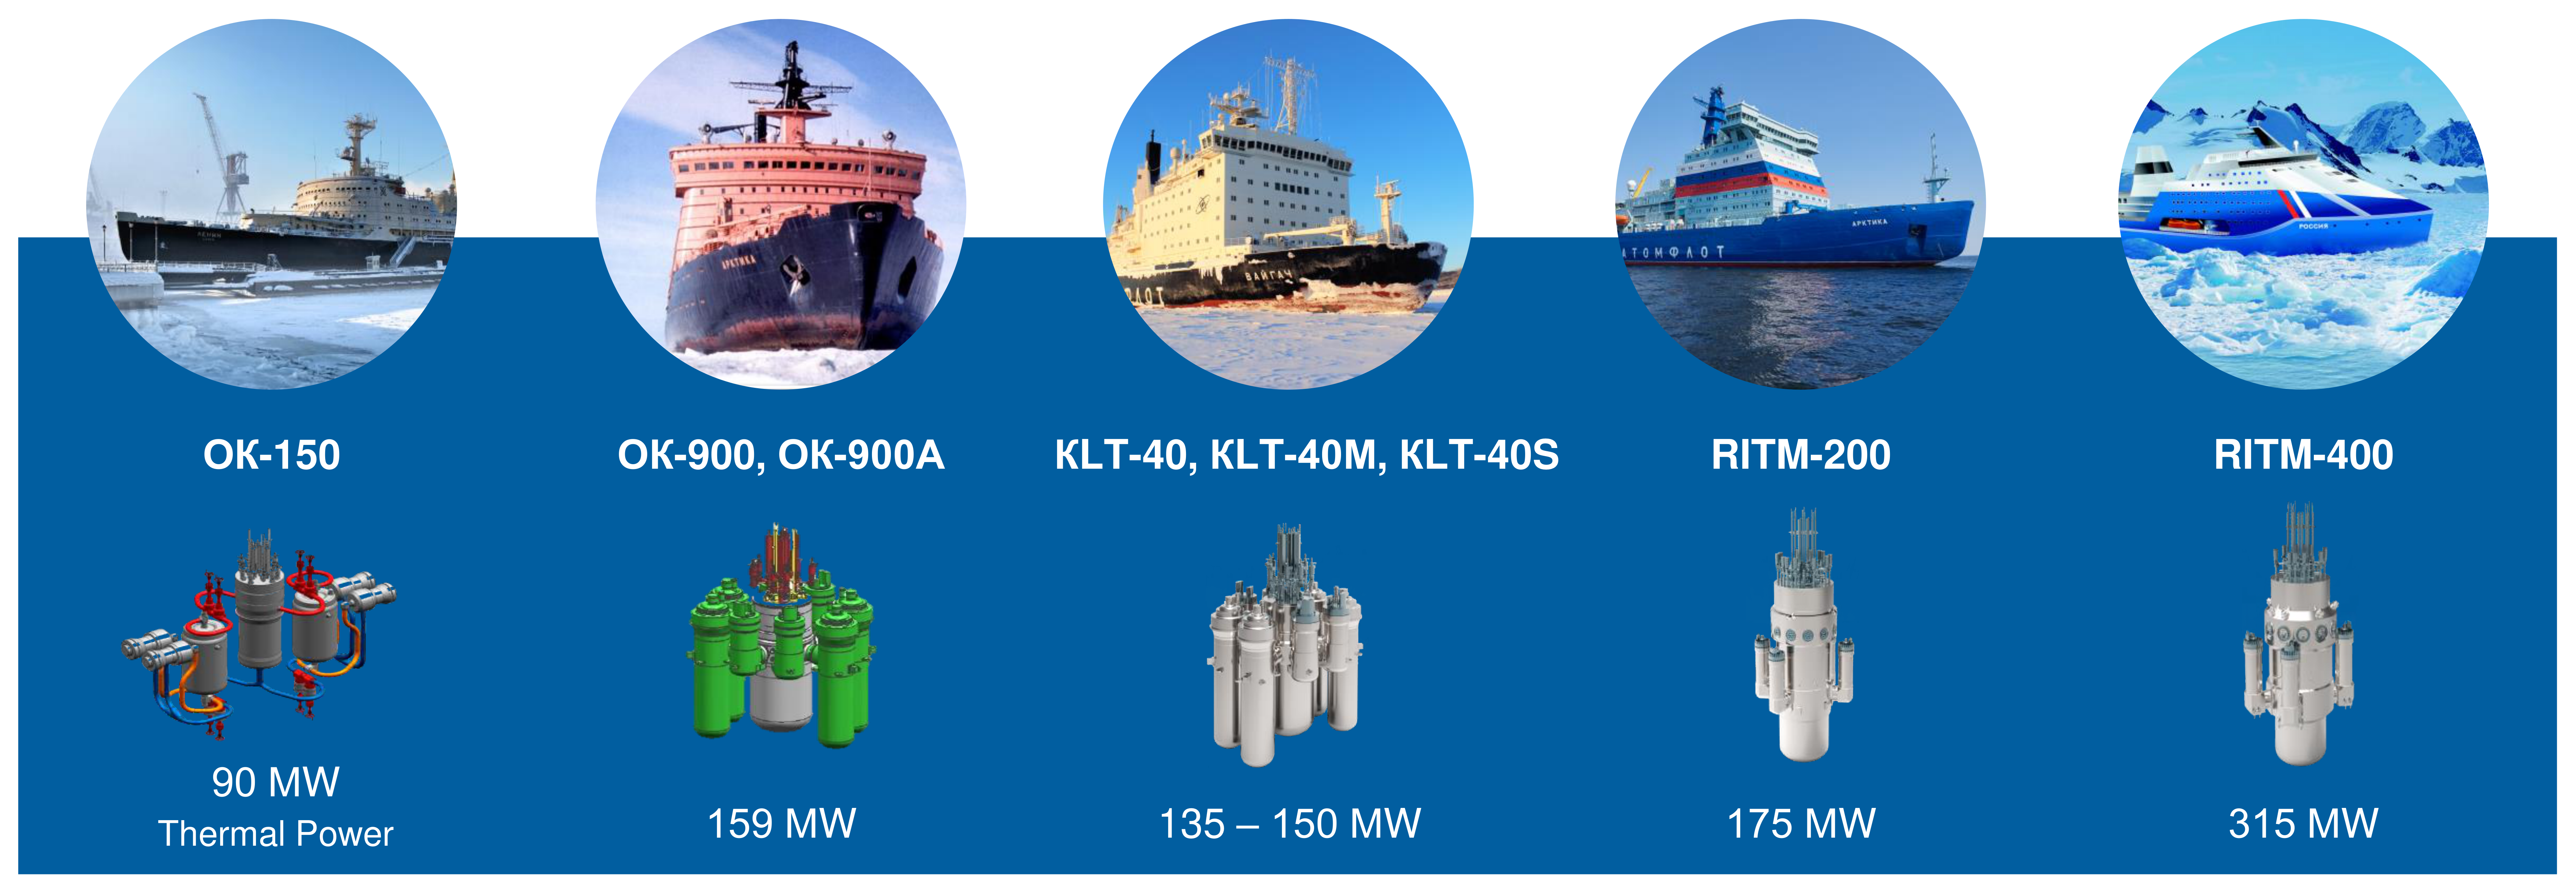
\includegraphics[width=\textwidth]{images/lr_okbm_icebreaker_reactors.png}
  \caption[Afrikantov OKBM reactors for nuclear icebreakers]{Afrikantov OKBM reactors for nuclear icebreakers.\newline Figure taken from~\cite{rosatom_presentation}.}
  \label{fig:lr-okbm-reactors}
\end{figure}

Two members of this line are documented in sufficient detail to be
useful here:

\begin{itemize}
  \item The KLT-40S is deployed in the floating nuclear power plant
        (FNPP) \emph{Akademik Lomonosov}. It uses uranium dioxide
        (UO$_2$) dispersed in a silumin matrix at 18.6~wt\% uranium-235,
        a core of 121 fuel assemblies, and a refuelling cycle of 30 to
        36 months~\cite{worldnuclearreport_smr}.

  \item The RITM-200N, the land-based member of the family, is rated
        190~MWth and 55~MWe gross and uses uranium enriched below
        20~wt\%~\cite{ritm200n_nei_2024}.
\end{itemize}

The relevance of the RITM-200N to this work is that its designers
describe its fuel cassettes as analogues of those used in the cores of
the RITM-200 and KLT-40S icebreakers~\cite{ritm200n_nei_2024}. The
transfer of a marine core to a land-based prototype is therefore
established practice, and the Brazilian programme follows it.

\subsubsection{The French lineage}
\label{subsec:lineage-france}
The K15 is an integral pressurised water reactor of 150~MWth. It and
its successor are used as follows~\cite{wna_ships}:

\begin{itemize}
  \item Two K15 units power the aircraft carrier \emph{Charles de
        Gaulle}, which runs five years between refuellings.

  \item The Le~Triomphant ballistic missile submarines use the same
        reactor.

  \item The Barracuda submarines carry 150~MWth reactors based on the
        K15, with a refuelling interval of about ten
        years~\cite{wna_ships}.
\end{itemize}

Newer French naval reactors run
on low-enriched uranium (LEU), at 7.5~wt\% in the Caramel fuel and about
5 to 6~wt\% in the Barracuda class~\cite{wna_ships}. The French line is the closest Western analogue to the present work.
Its naval propulsion cores operate below the 20~wt\% threshold that
separates LEU from highly enriched uranium (HEU)~\cite{nrc_10cfr110_2}.

\subsubsection{The United States and United Kingdom lineage}
\label{subsec:lineage-us-uk}
Naval reactors of the United States and the United Kingdom use
weapon-grade HEU. The enrichment is 93 to 97~wt\% uranium-235 in current
United States practice~\cite{jason_2016}, and it was 97.3~wt\% in United
States and British submarines in 1990~\cite{ippolito_1990}.

The feasibility of converting these cores to LEU at 19.75~wt\% has been
examined in two open assessments:

\begin{itemize}
  \item The report of the JASON advisory panel assessed the low-enriched
        fuel concept proposed by the Naval Nuclear Propulsion Program and
        the plan to develop and qualify it~\cite{jason_2016}.

  \item The report of the Office of Naval Reactors to Congress set out a
        conceptual research and development plan for a low-enriched naval
        fuel~\cite{onr_leu_2016}.
\end{itemize}

The second report assumes LEU at 19.75~wt\%, the highest enrichment
within the internationally recognised definition of
LEU~\cite{onr_leu_2016}. This work adopts 19.75~wt\% as the upper bound
of the enrichment range at the start of the optimisation study of the
core.

\subsubsection{The Brazilian lineage}
\label{subsec:lineage-brazil}
The Programa Nuclear da Marinha of the Brazilian Navy began in
1979~\cite{vasconcelos_fapesp_2025}. It is divided into two main
undertakings~\cite{marinha_relatorio_gestao_2025}:

\begin{itemize}
  \item The development of nuclear technology in the area of reactors.

  \item The mastery of the nuclear fuel cycle.
\end{itemize}

These two undertakings support the development and operation of the
land-based prototype of an embarked nuclear plant and of the plant of
the nuclear-powered submarine itself~\cite{marinha_relatorio_gestao_2025}.
That prototype is LABGENE, the Laboratório de Geração de Energia
Nucleoelétrica~\cite{marinha_relatorio_gestao_2025}. It is the
land-based prototype for the reactor of the submarine Álvaro
Alberto~\cite{vasconcelos_fapesp_2025} and is located at the Centro
Industrial Nuclear de Aramar (Cina) in Iperó, São
Paulo~\cite{ctmsp_visita_2018,vasconcelos_fapesp_2025}.

Figure~\ref{fig:vessel-components} identifies the components of a
pressurised water reactor vessel on the envelope adopted for the
LABGENE-class model. The envelope follows the simplified vessel drawing
prepared for a structural analysis according to the Centro
Tecnológico da Marinha em São Paulo (CTMSP)~\cite{maruyama_2013}.

The internals, the coolant path and the control rods in the figure are
illustrative and are not to scale. The coolant enters at the inlet
nozzle, descends the downcomer, passes through the lower plenum and the
core, and leaves at the outlet nozzle.

\begin{figure}[htbp]
  \centering
  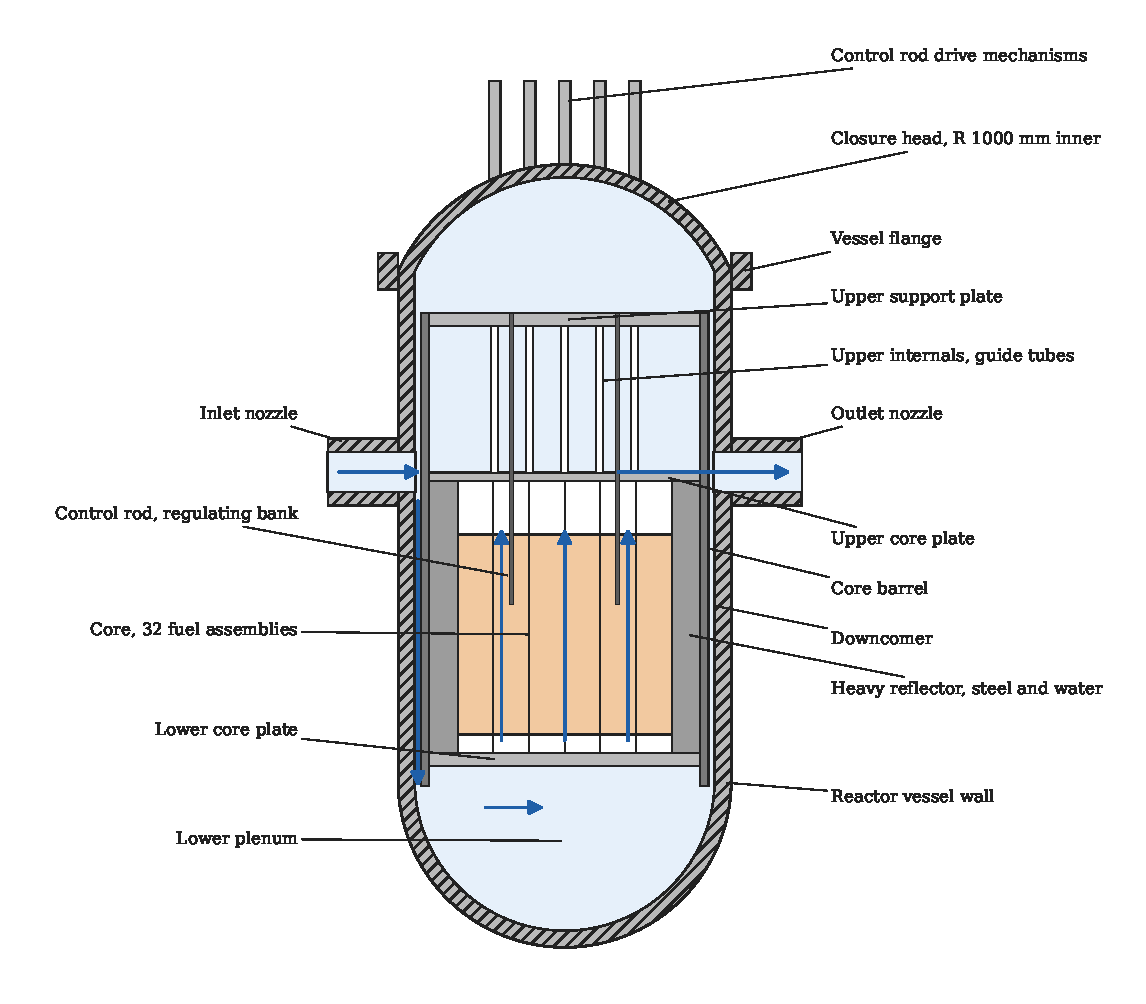
\includegraphics[width=0.95\textwidth]{images/th_vessel_components}
  \caption[Components of a pressurised water reactor vessel]{Components of a pressurised water reactor vessel, drawn on the LABGENE-class vessel envelope.\newline Vessel envelope adapted from~\cite{maruyama_2013}.}
  \label{fig:vessel-components}
\end{figure}

The open record establishes the following facts about the LABGENE
plant:

\begin{itemize}
  \item It is a pressurised water reactor with primary, secondary and
        cooling circuits, developed by the Navy for the submarine and
        tested first on land~\cite{ctmsp_labgene_2015}.

  \item According to the Navy, as reported by the specialised press, the
        reactor generates 48~MW of thermal
        power~\cite{demartini_nuclep_2022}, equivalent to 11~MWe for the
        prototype~\cite{galante_podernaval_2020}. The academic literature
        gives 48 to 50~MWth for the submarine
        reactor~\cite{dinizcosta_2017}.

  \item Its fuel is low-enriched uranium, as declared by Brazil at the
        2026 Review Conference of the Non-Proliferation
        Treaty~\cite{brazil_npt_wp13_2026}. The fuel consists of UO$_2$
        pellets in rods grouped into fuel
        elements~\cite{marinha_inb_labgene_2022,pereira_rmb_2023}.
        Ind\'ustrias Nucleares do Brasil (INB) produced the pellets of
        the LABGENE fuel between August and December
        2021~\cite{marinha_inb_labgene_2022}.

  \item The submarine will be a nuclear-powered, conventionally armed
        vessel. The land-based prototype reactor, the submarine, its
        reactor and its fuel are designed and built in
        Brazil~\cite{brazil_npt_wp13_2026}.

  \item The submarine is named \'Alvaro Alberto and is part of the
        Programa de Desenvolvimento de Submarinos (PROSUB), a partnership
        between Brazil and France~\cite{vasconcelos_fapesp_2025}.
\end{itemize}

The enrichment of the LABGENE fuel is reported inconsistently in open
sources:

\begin{itemize}
  \item In 2014 the chairman of the Navy's nuclear-propelled submarine
        development programme told the Foreign Relations and National
        Defence Committee of the Federal Senate that the fuel would be
        enriched to 6 to 8~wt\%~\cite{dinizcosta_2017}.

  \item Kassenova reported 18 to 19~wt\%~\cite{kassenova_2014}, a figure
        given by a former chairman of the Comiss\~ao Nacional de Energia
        Nuclear in 2005~\cite{dinizcosta_2017}.

  \item In 2025 Pesquisa FAPESP reported from Aramar that the submarine
        fuel enrichment will reach 19~wt\%. It quoted the director of
        CTMSP stating that the first fuel load had already been
        produced~\cite{vasconcelos_fapesp_2025}.
\end{itemize}

The refuelling interval is given as five years~\cite{dinizcosta_2017},
but no lattice pitch, assembly count, burnable poison loading, soluble
boron concentration or peaking factor for the LABGENE core is available
from any open source. The only open geometric information is the simplified
vessel drawing published in a structural dissertation carried out for
CTMSP. It gives the following dimensions~\cite{maruyama_2013}, shown in
Figure~\ref{fig:lr-maruyama-vessel}:

\begin{itemize}
  \item A cylindrical inner radius of 900~mm.

  \item A wall thickness of 100~mm.

  \item An overall height of 4700~mm.
\end{itemize}

\begin{figure}[htbp]
  \centering
  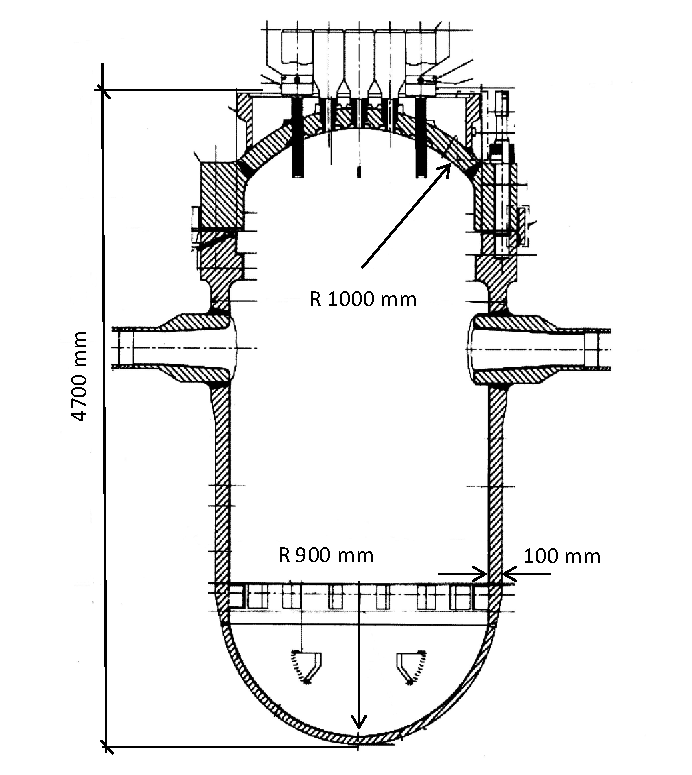
\includegraphics[width=0.55\textwidth]{images/lr_maruyama_vessel.pdf}
  \caption[Vessel dimensions adopted according to CTMSP]{Reactor vessel dimensions adopted according to CTMSP.\newline Figure taken from~\cite{maruyama_2013}.}
  \label{fig:lr-maruyama-vessel}
\end{figure}

Because the core data are closed, the present work is framed as a study
of a LABGENE-class core. Four inputs are taken from the open record:

\begin{itemize}
  \item The rated power.

  \item The PWR architecture.

  \item The low-enriched fuel.

  \item The vessel envelope.
\end{itemize}

Every remaining core parameter is an independent modelling choice of
this thesis and carries no claim of correspondence with the actual
prototype. These parameters are the following:

\begin{itemize}
  \item The enrichment zoning.

  \item The lattice pitch.

  \item The assembly count.

  \item The gadolinia (Gd$_2$O$_3$) loading.

  \item The poisoned-pin count.

  \item The reflector thickness.
\end{itemize}

The enrichment range at the start of the study, 2.0 to 19.75~wt\%, was
set from the open information and encloses the whole range reported for
the prototype. The
final campaign, constrained by the controllability screen of
Section~\ref{sec:meth-ctrl}, admits assembly enrichments up to
13.9~wt\%. The 19~wt\% reported for the prototype therefore lies inside
the explored range but outside the final candidate space.

\subsection{Open academic analyses}
\label{subsec:naval-academic}

Two bodies of open academic work give design data for compact
low-enriched cores. This thesis uses them for two questions: how
enrichment, core size and core life trade against each other, and how
far the power density and peaking of a boron-free marine core can go.

\subsubsection{Ippolito's comparison of submarine cores}
\label{subsec:academic-ippolito}

The thesis of Ippolito asked what a submarine core loses, in size and
in life, when its fuel changes from highly enriched to low-enriched
uranium~\cite{ippolito_1990}. Three cores of the same thermal power,
50~MWth, were designed to answer it. That power is close to the
48~MWth of the LABGENE-class core.

The three cores differ in the enrichment and in the form of their fuel.
Table~\ref{tab:lr-ippolito} shows what each one achieves.

\begin{table}[!htbp]
  \centering
  \caption{Submarine cores of 50~MWth compared by Ippolito: fuel, size and core life.}
  \label{tab:lr-ippolito}
  \small
  \begin{tabular}{@{}cccc@{}}
    \toprule
    Enrichment & Fuel & Core volume & Core life \\
    (wt\% $^{235}$U) & & (L) & (full-power days) \\
    \midrule
    7    & UO$_2$, caramel   & 506 & 600  \\
    20   & UO$_2$, caramel   & 667 & 1200 \\
    97.3 & UO$_2$/Zr cermet  & 265 & 1200 \\
    \bottomrule
  \end{tabular}

  \vspace{2pt}
  {\footnotesize Data from~\cite{ippolito_1990}.}
\end{table}
\FloatBarrier

The table reads as follows~\cite{ippolito_1990}:

\begin{itemize}
  \item \textbf{Same life, larger core:} the 20~wt\% core lasts as long as
        the 97.3~wt\% core, 1200 full-power days, which is about 3.3
        years at full power. It needs about two and a half times the
        volume, 667~L against 265~L.

  \item \textbf{Lower enrichment, shorter life:} the 7~wt\% core cannot
        stay critical for 1200 full-power days and lasts 600.

  \item \textbf{A manageable size penalty:} the 20~wt\% core is 24~cm wider
        and 30~cm taller than the 97.3~wt\% core. Ippolito judged that an
        integral reactor, with the steam generators inside the pressure
        vessel, can compensate for that increase.
\end{itemize}

The study also shows that the placement of the gadolinia changes its
effect~\cite{ippolito_1990}:

\begin{itemize}
  \item Mixed uniformly into the fuel, gadolinia reduced the reactivity
        to be controlled at the beginning of the cycle, but it burned out
        quickly because nothing shielded it from the neutrons.

  \item Concentrated in separate plates, gadolinia gave a peak of excess
        reactivity near the end of the cycle.
\end{itemize}

This thesis takes two points from the study. A 50~MWth core on
low-enriched uranium can last several years, at the price of a larger
core. The way the gadolinia is distributed in the fuel decides how its
hold-down changes through the cycle.

\subsubsection{The Cambridge studies of civil marine cores}
\label{subsec:academic-cambridge}

The Cambridge studies designed a soluble-boron-free PWR core for civil
marine propulsion with a life of 15 effective full-power years and fuel
below 20\%~$^{235}$U. Two of them are used here, in support of the
long-life, boron-free and heavily poisoned design logic of
Section~\ref{subsec:comparison} and of the power density entries of
Table~\ref{tab:naval-vs-commercial}:

\begin{itemize}
  \item The first part of the core design study works at assembly
        level, on the fissile loading, the burnable poisons and the
        control rods~\cite{alam_partI_2019}. The high fissile loading
        needed for the long life makes the beginning-of-life reactivity
        very high. A self-shielded burnable absorber keeps the assembly
        reactivity low and stable with relatively little burnup
        penalty~\cite{alam_partI_2019}.

  \item The hot channel analysis coupled neutronics and thermal
        hydraulics for a 375~MWth version of the core, with 16\% UO$_2$
        and 19.25\% duplex fuel~\cite{alam_2019_hotchannel}. The average
        power density of the reference core, about 63~MW/m$^3$, could
        be raised to 100~MW/m$^3$ while every thermal-hydraulic limit was
        met. At 111~MW/m$^3$ the surface heat flux, the fuel temperature
        and the pressure drop exceeded their limits. Power peaking stayed
        below the industry limit of 1.5, and the minimum departure from
        nucleate boiling ratio was not the limiting
        factor~\cite{alam_2019_hotchannel}.
\end{itemize}

\subsection{Comparison of naval-heritage and commercial small modular PWR cores}
\label{subsec:comparison}

Table~\ref{tab:naval-vs-commercial} contrasts the two design families on
the characteristics most relevant to core and fuel design. Every entry
is traceable to a named open source. The detailed criteria of classified
naval programmes are not verifiable in open sources.

\begin{table}[htbp]
  \centering
  \footnotesize
  \caption{Naval-heritage and commercial small modular PWR cores: design characteristics.}
  \label{tab:naval-vs-commercial}
  \begin{tabularx}{\textwidth}{@{}>{\raggedright\arraybackslash}p{2.8cm} >{\raggedright\arraybackslash}X >{\raggedright\arraybackslash}X@{}}
    \toprule
    \textbf{Characteristic} & \textbf{Naval-heritage core} &
    \textbf{Commercial SMR core} \\
    \midrule
    Fuel enrichment &
    HEU of 93 to 97~wt\% in US and UK practice~\cite{jason_2016}, and LEU
    below 10~wt\% in French submarines~\cite{ippolito_1990}. 18.6~wt\% in
    the KLT-40S~\cite{worldnuclearreport_smr} &
    LEU below 5~wt\%~\cite{iaea_smr_2024}, up to 4.95~wt\% in the NuScale
    fuel design~\cite{nuscale_htp2_2017} \\
    \addlinespace
    Refuelling interval &
    30 to 36 months for the KLT-40S~\cite{worldnuclearreport_smr}. Five
    years for the \emph{Charles de Gaulle} and about ten years for the
    K15-based Barracuda reactors~\cite{wna_ships} &
    18 to 24 months~\cite{iaea_smr_2024} \\
    \addlinespace
    Soluble boron &
    Soluble-boron-free operation proposed for civil marine
    cores~\cite{alam_partI_2019} &
    Borated coolant, with boron-free variants such as the ACP100 and the
    i-SMR~\cite{acp100_physor2020,ismr_sbf_2024} \\
    \addlinespace
    Burnable poison &
    A major share of the hold-down of a high beginning-of-life
    reactivity~\cite{alam_partI_2019,ippolito_1990} &
    Gd$_2$O$_3$ up to 8~wt\% in the NuScale fuel
    design~\cite{nuscale_htp2_2017} \\
    \addlinespace
    Power density &
    Up to about 100~MW/m$^3$~\cite{alam_2019_hotchannel} &
    60 to 65~MW/m$^3$~\cite{alam_2019_hotchannel} \\
    \addlinespace
    Motion and shock &
    Qualified for inclination, motion and shock~\cite{ritm200n_nei_2024} &
    Land-based siting~\cite{iaea_smr_2024} \\
    \addlinespace
    Reactivity control &
    Control rods with compensating groups~\cite{worldnuclearreport_smr} &
    Control rods plus soluble boron, or rods plus burnable poison in
    boron-free designs~\cite{acp100_physor2020,ismr_sbf_2024} \\
    \bottomrule
  \end{tabularx}
\end{table}

The differences collected in Table~\ref{tab:naval-vs-commercial} follow
from a small set of naval operational requirements. Each requirement
has a consequence for the core:

\begin{enumerate}
  \item Energy autonomy without frequent refuelling asks for a compact
        core with a large energy reserve, which higher enrichment
        provides~\cite{ippolito_1990}.

  \item High availability at sea asks for long refuelling intervals. The
        fissile loading needed for a long life gives a high
        beginning-of-life reactivity~\cite{alam_partI_2019}.

  \item Soluble-boron-free operation simplifies the plant and saves
        space. It removes the corrosive effect of the boron, improves the
        moderator temperature coefficient and eliminates boron dilution
        accidents, including dilution by seawater if the ship
        sinks~\cite{alam_partI_2019}.

  \item Heavy reliance on movable rods is avoided, so the burnable poison
        carries a major part of the reactivity control. A self-shielded
        absorber keeps the assembly reactivity low and stable with little
        burnup penalty~\cite{alam_partI_2019}.

  \item Compactness within the hull raises the volumetric power density
        and tightens the margin to the hot channel limit expressed by
        $F_{\Delta H}$~\cite{alam_2019_hotchannel}.

  \item A ship must also vary its power easily~\cite{alam_partI_2019},
        which in a boron-free core falls to the regulating rods.

  \item Qualification for inclination, motion and shock adds structural
        and thermal-hydraulic margins~\cite{ritm200n_nei_2024}. It is
        recorded in the table for completeness and is not acted on in
        this work, whose model carries no thermal-hydraulic feedback.
\end{enumerate}

Four of these requirements enter the design space and the objectives of
this thesis:

\begin{itemize}
  \item The enrichment.

  \item The burnable poison inventory.

  \item The boron strategy.

  \item The power density.
\end{itemize}

\subsection{Positioning of the LABGENE-class 48\texorpdfstring{\,}{ }MWth core}
\label{subsec:positioning}

The core studied in this thesis is a LABGENE-class 48~MWth pressurised
water reactor of naval heritage. Among designs with open documentation,
the closest operating analogues are the KLT-40S and the RITM-200 family.
They share the naval logic of a compact low-enriched-uranium core with a
long refuelling
interval~\cite{worldnuclearreport_smr,ritm200n_nei_2024}.

The core would drive the land-based propulsion prototype at LABGENE,
whose visual mock-up is shown in Figure~\ref{fig:lr-labgene-blocks}.
The plant is arranged in three blocks, listed below from the reactor
outwards~\cite{galante_podernaval_2020b}:

\begin{itemize}
  \item Block 40 holds the primary circuit: the reactor pressure vessel,
        the steam generators, the pressuriser and the primary pumps.

  \item Block 30 holds the secondary circuit: the turbogenerators with
        their lubrication system, the condenser and the steam generator
        feedwater pumps.

  \item Block 20 holds the propulsion line: the electric propulsion
        motor, the speed-increasing gearbox and the dynamometer brake that
        absorbs the shaft power in place of a propeller.
\end{itemize}

\begin{figure}[htbp]
  \centering
  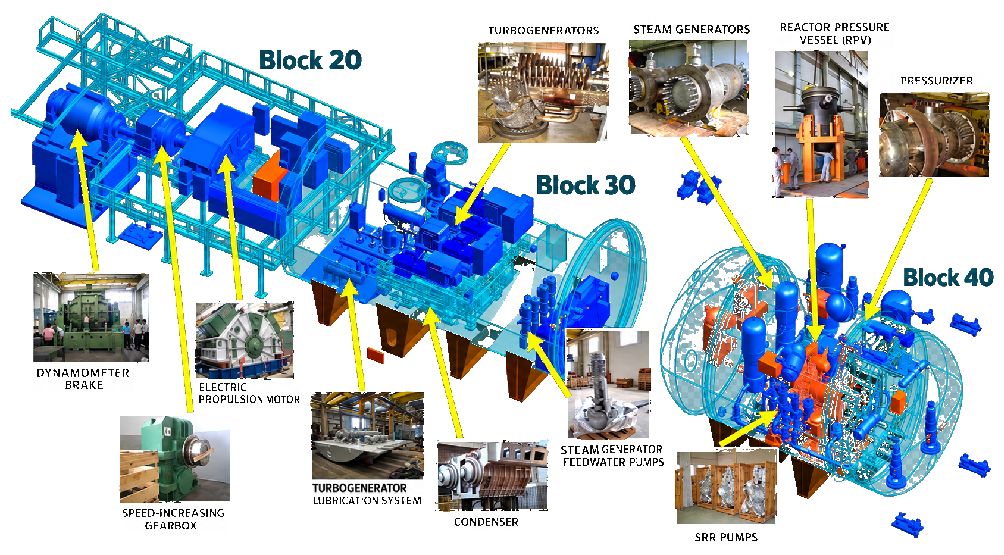
\includegraphics[width=\textwidth]{images/lr_labgene_blocks.pdf}
  \caption[Mock-up of the LABGENE land-based prototype]{Visual mock-up of the LABGENE land-based prototype.\newline Figure adapted from~\cite{galante_podernaval_2020b}.}
  \label{fig:lr-labgene-blocks}
\end{figure}

The optimisation objectives map directly onto the naval requirements:

\begin{itemize}
  \item The cycle length maps onto the requirement of long core life.

  \item The radial enthalpy-rise hot channel factor $F_{\Delta H}$ maps
        onto compact high-power-density operation.
\end{itemize}

The design variables are the levers of a long-life core, namely the
fissile loading, the burnable absorber and the geometry of the lattice
and of the reflector. The soluble boron is held constant at the
1000~ppm of the NuScale-like benchmark from which the assembly geometry
is taken, and the constraint on the beginning-of-life multiplication
factor is applied with that boron present
(Section~\ref{sec:meth-boron}). The design variables are the following:

\begin{itemize}
  \item The enrichment.

  \item The gadolinia concentration and the poisoned-pin count.

  \item The pin pitch.

  \item The reflector thickness.
\end{itemize}

The enrichment range explored in Campaigns 1 to 6, 2.0 to 19.75~wt\%,
encloses every figure reported for the prototype. Those figures range
from the 6 to 8~wt\% stated in 2014~\cite{dinizcosta_2017} to the
19~wt\% reported in 2025~\cite{vasconcelos_fapesp_2025}, so the
optimisation does not presuppose any of them.

The controllability screen of the final campaign then bounds the
candidate space at 13.9~wt\%, below the highest reported figure. That
bound is itself a result on the prototype envelope.

\section{Optimisation of nuclear reactor cores: development and state
of the art}
\label{sec:lit-opt}

Section~\ref{sec:smr-naval} fixed the design envelope of the core
studied here: its thermal power, its fuel class, the vessel that bounds
it and the refuelling interval it has to meet. Those quantities enter
the present work as fixed input data and as constraints on the design
space. This section reviews the methods by which a core is optimised
within such an envelope.

Fuel reloading and core design optimisation keep the cycle length, the
power level and the feedback within their targets by choosing the
following quantities~\cite{stewart_2021}:

\begin{itemize}
  \item The arrangement of the assemblies.

  \item The core geometry.

  \item The material composition.
\end{itemize}

The field has six decades of history, and its methods track the wider
history of engineering optimisation. The review proceeds in three
parts:

\begin{enumerate}
  \item The chronological development of the methods, from mathematical
        programming to machine learning
        (Sections~\ref{sec:lit-opt-early} to
        \ref{sec:lit-opt-surrogate}).

  \item The structural difficulties of the field, above all the
        difficulty introduced by burnup
        (Sections~\ref{sec:lit-opt-difficulties}
        and \ref{sec:lit-opt-burnup}).

  \item The current state of the art, with the strengths and
        limitations of each family of methods and the positioning of
        the present work (Section~\ref{sec:lit-opt-sota}).
\end{enumerate}

\subsection{Mathematical programming and the Haling principle}
\label{sec:lit-opt-early}

Mathematical programming was applied to in-core fuel management in
three forms:

\begin{itemize}
  \item Dynamic programming, in the work of Wall and Fenech in
        1965~\cite{meneses_2010}.

  \item Linear and quadratic programming, in the work of Tabak in
        1968~\cite{meneses_2010}.

  \item Linear programming for the refuelling schemes of light water
        reactors, and optimal control for the time-dependent management
        of the control poison~\cite{downar_1988}.
\end{itemize}

The most influential idea of the era is the Haling principle. If the
power in each region is held constant through the cycle, the depletion
follows a straight line in reactivity space and the power peaking can be
no higher or lower at any point of the cycle. That constant shape gives
the minimum peaking, and the end-of-cycle state follows from a single
depletion~\cite{downar_1988}.

The principle became the standard shortcut of the period because it
removed the need to march every candidate design through time. Its use
rests on the assumption that the Haling power distribution closely
resembles the power shape of the final, detailed core
design~\cite{downar_1988}.

The deterministic era carried a structural weakness. Linear programming
uses only first derivatives of the objective and cannot distinguish a
local from a global optimum, so different starting points can return
different solutions~\cite{downar_1988}. This is a serious limitation in
a design space that is discrete, nonconvex and rich in local optima.

\subsection{Heuristics, knowledge-based systems and perturbation
theory}
\label{sec:lit-opt-heuristic}

The 1980s produced two complementary responses to that mismatch. The
first automated the search itself. Hobson and Turinsky determined
the loading pattern that maximises beginning-of-cycle reactivity under
power peaking and discharge burnup constraints. Their method combined
two tools~\cite{hobson_turinsky_1986}:

\begin{itemize}
  \item Monte Carlo integer programming as the search.

  \item First-order perturbation theory to estimate the effect of each
        assembly shuffle.
\end{itemize}

Designer knowledge was also encoded directly. Logical rules for
generating loading patterns appear as early as 1972, and expert systems
became one of three kinds of decision-support
tool~\cite{meneses_2010}:

\begin{itemize}
  \item Manual design packages.

  \item Optimisation packages.

  \item Expert systems.
\end{itemize}

The second response was generalised perturbation theory (GPT). GPT
estimates how the core eigenvalue and the power distribution respond to
a fuel shuffle without a full re-solution of the transport problem. It
was demonstrated for three-dimensional design optimisation of Canada
Deuterium Uranium (CANDU) reactors~\cite{rozon_beaudet_1992}.

GPT then became the neutronics engine of the FORMOSA-P code. There a
nodal GPT model evaluates objectives and constraints cheaply enough to
sit inside a stochastic search, and the method was extended even to the
feed enrichment as a decision variable~\cite{maldonado_1995}. That model
is of higher order, because first-order perturbation techniques proved
inadequate for loading pattern changes~\cite{maldonado_1995}.

Perturbation methods have known limits:

\begin{itemize}
  \item First-order perturbation theory is accurate only for small
        changes from the reference state~\cite{hobson_turinsky_1986}.

  \item Depletion perturbation theory cannot accurately represent
        assembly movement or the strong flux perturbations introduced
        by burnable absorbers~\cite{downar_1988}.
\end{itemize}

\subsection{Stochastic global search}
\label{sec:lit-opt-stochastic}

At the turn of the 1990s, the field accepted that the design space is
nonconvex and moved to stochastic global search. Kropaczek and Turinsky combined simulated annealing with a core physics
model based on second-order generalised perturbation theory for PWR
reload design. Their code places the feed fuel, the burnt fuel with its
orientation and the burnable poisons to reach one of three objectives,
with the limits on peaking, burnup and moderator temperature coefficient
enforced either by penalty functions or by rejecting the exchanges that
violate them~\cite{kropaczek_turinsky_1991}:

\begin{itemize}
  \item Maximise the multiplication factor at a target end-of-cycle
        burnup.

  \item Minimise the maximum radial power peaking over the cycle.

  \item Maximise the discharge burnup.
\end{itemize}

Genetic algorithms, which evolve a population of candidate solutions by
mimicking natural selection~\cite{deb_2001}, entered the field shortly
after. Poon and Parks applied them to the positions and orientations of
the fuel assemblies together with their burnable poison, and tabu search
was applied with similar success~\cite{meneses_2010}.

At the end of the decade, Yamamoto compared these heuristics on equal
terms. A single benchmark, the loading pattern of a Westinghouse
three-loop PWR of 900~MWe with 157 assemblies, was solved ten times with
each method, with the aim of maximising the cycle length while keeping
the radial peaking factor below 1.435. The comparison gave the following
results~\cite{yamamoto_1997}:

\begin{itemize}
  \item Direct search and binary exchange evaluated the fewest loading
        patterns, but they were trapped in local optima and reached the
        lowest quality.

  \item Simulated annealing and the genetic algorithm reached better
        patterns. The slowest cooling schedule of simulated annealing
        needed about 10\,300 evaluated patterns on average, against 3000
        for the genetic algorithm.

  \item A hybrid of the genetic algorithm with binary exchange performed
        best, because the global search of the first and the local search
        of the second compensated for each other's weaknesses.
\end{itemize}

For the present work, the most relevant result of the period is the
first nondominated genetic search for PWR reload
design~\cite{parks_1996}. Parks applied it to the reload core of a
Westinghouse three-loop PWR, with three objectives optimised at the same
time~\cite{parks_1996}:

\begin{itemize}
  \item Minimise the feed enrichment.

  \item Maximise the discharge burnup.

  \item Minimise the radial form factor.
\end{itemize}

The usual alternative adds the objectives into one weighted function.
Each run then returns a single design, whose position on the trade-off
depends on the weights the designer chose, so the trade-off can only be
explored with many runs~\cite{parks_1996}.

The nondominated search ranks the designs of its population by Pareto
dominance and keeps an archive of the designs that no other design beats
in every objective. One run therefore returns the whole trade-off
surface, and the designer picks from it the designs worth closer
study~\cite{parks_1996}.

This is the Pareto-based formulation that the Non-dominated Sorting
Genetic Algorithm II (NSGA-II) later standardised~\cite{deb_nsga2_2002}.
\textbf{This thesis adopts it}, so its result is a Pareto front of possible core
designs and the choice among them is left to the designer.

\subsection{Population-based metaheuristics and multi-objective
evolutionary algorithms}
\label{sec:lit-opt-population}

The 2000s and 2010s widened the toolbox with swarm algorithms. The survey
of Stewart, Palmer and DuPont reports three examples~\cite{stewart_2021}:

\begin{itemize}
  \item Yadav and Gupta (2011) applied particle swarm optimisation to
        find PWR core configurations with reasonably low peaking factors,
        using a conventional neutron transport solver and no surrogate
        model.

  \item Safarzadeh et al.\ (2014) used a hybrid bee colony algorithm to
        reduce the time needed to find reload patterns for the core of a
        VVER-1000 pressurised water reactor, in comparison with a standard
        particle swarm optimisation.

  \item Domingos, Schirru and Pereira (2006) found particle swarm
        optimisation easier to model than evolutionary methods, and less
        costly for the same results on simplified core geometries.
\end{itemize}

Brazilian researchers of the COPPE/UFRJ group, at the Federal University
of Rio de Janeiro, worked on the reload optimisation problem of Angra~1,
a Westinghouse pressurised water reactor in commercial operation at Angra
dos Reis, Brazil, since 1985~\cite{eletronuclear_angra1}. At each
refuelling, part of the fuel is replaced, and the assemblies are
rearranged, and the group used the seventh operating cycle of the plant
as a common test case for choosing that arrangement. Four methods were
applied to it and compared~\cite{meneses_2010}:

\begin{itemize}
  \item The Ant-Q ant colony algorithm.

  \item Artificial ant colony connective networks.

  \item Population-based incremental learning.

  \item Particle swarm optimisation with random keys.
\end{itemize}

On the multi-objective side, NSGA-II~\cite{deb_nsga2_2002} and SPEA are
the two multi-objective genetic algorithms most widely used in
research~\cite{stewart_2021}. They rest on the broader theory of
multi-objective evolutionary algorithms
(MOEAs)~\cite{deb_2001,coello_2007}.

An MOEA is a population-based search that applies the evolutionary
operators of selection, crossover and mutation to a set of candidate
designs. Because it processes a whole population at every iteration, its
outcome is also a population, and it can find several Pareto-optimal
solutions in one run without first merging the objectives into a single
function~\cite{deb_2001}. Such an algorithm pursues two goals at the same
time~\cite{deb_2001}:

\begin{itemize}
  \item Convergence, meaning a set of solutions as close as possible to
        the Pareto-optimal front.

  \item Diversity, meaning a set of solutions spread as widely as
        possible along that front.
\end{itemize}

In his book on multi-objective optimisation with evolutionary algorithms,
Deb (2001) classifies MOEAs by whether they preserve elitism, that is, whether
the best solutions of a population are carried directly into the next
generation. VEGA, MOGA, NSGA and NPGA are non-elitist algorithms, while
NSGA-II, SPEA and PAES preserve the elite~\cite{deb_2001}.

\subsection{Surrogate-assisted optimisation and machine learning}
\label{sec:lit-opt-surrogate}

The binding constraint of every method above is the number of calls to
the expensive simulator. Surrogate-assisted evolutionary computation
addresses it directly, in three steps~\cite{jin_2011}:

\begin{enumerate}
  \item A cheap statistical model is trained on evaluated designs.

  \item The optimiser searches the model.

  \item The simulator is reserved for the most informative candidates.
\end{enumerate}

Gaussian process regression is the canonical surrogate. Its prediction
carries an uncertainty that is reduced close to the evaluated designs
and grows away from them~\cite{rasmussen_gp_2006}.

The Gaussian process, known in engineering design as Kriging, suits
problems in which every sample comes from an expensive simulation. Such
samples must be used sparingly, and their number is often small because
each one carries a computational cost~\cite{forrester_book_2008}. Two
properties make the model a good choice in this setting:

\begin{itemize}
  \item It estimates its own error. The predictive variance shows where
        the model is uncertain, so new samples can be placed where they
        improve it most, which Forrester, Sobester and Keane call a key
        advantage of Gaussian process models~\cite{forrester_book_2008}.
        The Gaussian process is also the surrogate most often used to
        estimate model uncertainty in evolutionary
        optimisation~\cite{jin_2011}.

  \item Its cost is affordable for a modest data set. Exact Gaussian
        process prediction scales as $\mathcal{O}(n^3)$ with the number
        $n$ of training points, which becomes prohibitive for large data
        sets~\cite{rasmussen_gp_2006}. The guideline of Forrester,
        Sobester and Keane places Kriging models within reach for fewer
        than about 20 variables and 500 samples, and points to support
        vector regression, fixed radial basis functions or polynomials
        beyond that range~\cite{forrester_book_2008}.
\end{itemize}

The problem of this thesis falls inside that range. It has four to six
design variables, and each completed campaign evaluated between 36 and
114 designs, each one a Monte Carlo depletion. \textbf{For these reasons, a
Gaussian process was chosen as the surrogate model of this thesis.}

The loop is initialised by a space-filling sampling plan, which spreads
the first designs over the design space before any surrogate exists.
McKay, Beckman and Conover compared three ways of choosing these
inputs~\cite{mckay_lhs_1979}:

\begin{enumerate}
  \item Random sampling, in which the input vectors are drawn at random
        from their joint distribution.

  \item Stratified sampling, in which the sample space is divided into
        disjoint strata and a random sample is drawn from each stratum,
        so that every region of the space is represented.

  \item Latin hypercube sampling, in which the range of each variable is
        divided into $N$ intervals of equal probability, one value is
        drawn from each interval, and the values of the different
        variables are matched at random.
\end{enumerate}

In their comparison, Latin hypercube sampling estimated the mean, the
variance, and the distribution function of the output with a smaller
spread than the other two methods. It improves on random sampling when
certain monotonicity conditions hold~\cite{mckay_lhs_1979}.

After the initial plan, the loop is driven by infill criteria that
balance exploration against exploitation. A criterion such as the
expected improvement weighs the prediction of the surrogate against its
uncertainty, so new designs are placed both where the prediction is
promising and where the model knows least~\cite{forrester_book_2008}.

For multi-objective problems, the hypervolume indicator, the volume of
objective space weakly dominated by a front, measures the quality of
that front~\cite{zitzler_2003_performance}. It can also serve as the
target of the infill selection.

Surrogate-assisted search is the first of two recent frontiers in
nuclear core optimisation, and its applications are growing:

\begin{enumerate}
  \item Deep neural network surrogates coupled to NSGA-II for the loading
        patterns of a 36-assembly microcore, a 37-assembly small modular
        core and a 193-assembly PWR core~\cite{whyte_2020}.

  \item A convolutional neural network surrogate combined with a
        genetic algorithm for reload pattern
        optimisation~\cite{wan_2022}.

  \item Neural network acceleration of a genetic algorithm for a
        coupled fast and thermal experiment whose design space exceeds
        $3\times10^{71}$ configurations~\cite{pevey_2022}.
\end{enumerate}

Deep reinforcement learning is the second frontier, after the
surrogate-assisted search described above. The results below are
reported by the developing groups, and independent replication remains
limited:

\begin{itemize}
  \item Physics-informed reinforcement learning for assembly design is
        reported by its authors to find several times more feasible
        patterns than stochastic optimisation at a markedly lower
        computational cost~\cite{radaideh_2021_rl}.

  \item The NEORL framework packages these algorithms for energy
        applications. NEORL, short for NeuroEvolution Optimisation with
        Reinforcement Learning, is an open-source Python framework
        developed at the Massachusetts Institute of
        Technology~\cite{radaideh_2023_neorl}:

        \begin{itemize}
          \item It offers more than 30 algorithms from evolutionary
                computation, neural networks and neuroevolution, from
                genetic algorithms, particle swarm optimisation and
                simulated annealing to proximal policy optimisation and
                hybrid methods such as PESA.

          \item Most of its algorithms evaluate the population in
                parallel, which shortens the search when each evaluation
                runs a simulation code.

          \item Its nuclear demonstration optimised the loading pattern of
                a three-batch PWR core of 217 assemblies with the SIMULATE3
                nodal code, where PESA and proximal policy optimisation
                found more than 100 feasible patterns.
        \end{itemize}

  \item The Pareto Envelope Augmented with Reinforcement Learning (PEARL)
        approach is reported to reach a larger hypervolume than NSGA-III,
        multi-objective simulated annealing and multi-objective tabu
        search on a full-size PWR reload
        problem~\cite{seurin_2024_pearl}.
\end{itemize}

The following open-source codes complete the toolchain. Together they
make reproducible surrogate-assisted core optimisation feasible on modest
computing budgets, \textbf{the route taken by this thesis}:

\begin{itemize}
  \item OpenMC provides open-source Monte Carlo neutron
        transport~\cite{romano_openmc_2015} with an in-memory
        Python-coupled depletion capability~\cite{romano_2021_depletion}.

  \item scikit-learn, a Python module for machine learning
        algorithms~\cite{pedregosa_sklearn_2011}, provides the Gaussian
        process regression used as the surrogate model of this thesis.

  \item pymoo provides NSGA-II and its relatives in the same
        language~\cite{blank_deb_2020}.
\end{itemize}

Table~\ref{tab:lit-opt-timeline} condenses the six decades into a
timeline. Each row gives four items for one period:

\begin{itemize}
  \item The dominant method family.

  \item Its representative works.

  \item Its main contribution.

  \item The limitation that motivated the next period.
\end{itemize}

\begin{table}[htbp]
  \centering
  \caption{Optimisation methods in core design and in-core fuel management: timeline.}
  \label{tab:lit-opt-timeline}
  \footnotesize
  \begin{tabular}{@{}>{\raggedright\arraybackslash}p{0.105\textwidth}>{\raggedright\arraybackslash}p{0.155\textwidth}%
                  >{\raggedright\arraybackslash}p{0.215\textwidth}>{\raggedright\arraybackslash}p{0.21\textwidth}>{\raggedright\arraybackslash}p{0.20\textwidth}@{}}
    \toprule
    Period & Method family & Sources & Main contribution &
    Main limitation \\
    \midrule
    1960s and 1970s &
    Mathematical programming and the Haling principle &
    \cite{meneses_2010,downar_1988} &
    First formal problem statements and a single-pass depletion
    shortcut &
    Convexity assumptions and the constant-shape approximation \\
    \addlinespace
    1980s and early 1990s &
    Expert systems and perturbation theory &
    \cite{hobson_turinsky_1986,meneses_2010,rozon_beaudet_1992} &
    Fast response estimation inside search loops &
    First-order accuracy limited to small perturbations \\
    \addlinespace
    Late 1980s and 1990s &
    Simulated annealing, genetic algorithms and tabu search &
    \cite{kropaczek_turinsky_1991,maldonado_1995,parks_1996,meneses_2010} &
    Global search and the first Pareto reload design &
    Very high evaluation counts \\
    \addlinespace
    2000s and 2010s &
    Population-based metaheuristics and MOEAs &
    \cite{deb_nsga2_2002} &
    Full Pareto fronts in a single run &
    Cost-prohibitive with high-fidelity physics \\
    \addlinespace
    2019 to today &
    Surrogate-assisted search and deep reinforcement learning &
    \cite{whyte_2020,seurin_2024_pearl} &
    Sample efficiency and learned placement policies &
    Surrogate accuracy in high dimensions and heavy training cost \\
    \bottomrule
  \end{tabular}
\end{table}

\subsection{Specific difficulties of nuclear core optimisation}
\label{sec:lit-opt-difficulties}

Six structural features distinguish the optimisation of nuclear reactor
cores from generic engineering optimisation. Each one shaped the history above, and each
one acts on the pipeline of this thesis:

\begin{enumerate}
  \item \emph{Combinatorial size.} The number of loading patterns for
        $n$ assemblies approaches $n!$~\cite{stewart_2021}, and discrete
        choices coexist with continuous variables such as enrichment and
        dimensions. A recent design study reports more than
        $3\times10^{71}$ configurations for 150 positions and three
        candidate materials~\cite{pevey_2022}.

  \item \emph{Expensive evaluations.} Each candidate is scored by a
        reactor physics code. No analytical function gives the objectives
        of a design, so the optimiser can only run the simulation and read
        its results~\cite{jin_2011}. The cost of one run grows with the
        detail of the model:

        \begin{itemize}
          \item A Monte Carlo depletion of the two-dimensional fuel
                assembly used in this thesis takes fifteen to twenty-five
                minutes (Chapter~\ref{ch:methodology}).

          \item In a surrogate-assisted study of PWR fuel management, the
                burnup calculations took hours, and the depletion of a
                single fuel unit cell needed about 1.1 CPU hours per burnup
                step~\cite{whyte_2020}.

          \item A Monte Carlo evaluation of a depletion problem makes no
                approximations of its own, but it can take many hundreds
                of thousands of CPU hours~\cite{josey_2017}.
        \end{itemize}

        CPU hours are summed over all the processors of a run, so the
        elapsed time is shorter on a parallel machine. The affordable
        number of evaluations is still capped, which is the motivating
        premise of surrogate-assisted search~\cite{jin_2011}.

  \item \emph{Nonconvex and multimodal landscapes.} Objectives respond
        discontinuously to discrete changes, and the landscape is rich in
        local optima. An analysis of 300\,000 loading patterns found
        about one local optimum per hundred configurations, roughly
        $10^{11}$ local optima among the $10^{13}$ patterns of an
        octant-symmetric core. Gradient-based methods are therefore not
        adequate~\cite{meneses_2010}.

  \item \emph{Competing objectives under licensing constraints.} A reload
        must keep the desired cycle length while limiting the poison
        concentration and the power peaking~\cite{stewart_2021}. The
        safety limits enter as constraints next to these objectives.

  \item \emph{Stochastic objectives.} Monte Carlo simulators return
        objectives with statistical uncertainty. The noise perturbs the
        ranking of nearby designs and propagates through depletion
        steps, as developed in Section~\ref{sec:lit-opt-burnup}.

  \item \emph{The fidelity gap.} Cheap screening models rank designs
        differently from high-fidelity evaluation. The canonical
        statistical fusion of two fidelities is the autoregressive model
        of~\cite{kennedy_ohagan_2000}, with engineering practice
        in~\cite{forrester_book_2008}.

        A recurring caution is that the cross-fidelity correlation
        weakens near the optimum, exactly where an optimiser converges.
        The difficulty is old: in most of the work surveyed in 1988,
        improvements found with simplified core models were not realised
        in detailed licensing-type analysis~\cite{downar_1988}.

        This thesis measures the corresponding rank inversion between
        assembly-level and core-level evaluation in
        Chapter~\ref{ch:results}.
\end{enumerate}

\subsection{The burnup difficulty}
\label{sec:lit-opt-burnup}

Among these features, depletion is the one that defines the cost
structure of the problem, and it is the central methodological concern
of this work. A static figure of merit, such as the beginning-of-life
(BOL) power peaking, requires one transport solution per candidate.
Cycle length, end-of-cycle reactivity and discharge burnup are different
in kind.

These quantities depend on the whole time history of the core. Each
candidate therefore requires a full depletion simulation, in which a
transport solution gives the reaction rates for the current composition
and the composition is then advanced over a time step. The cost of one
evaluation is multiplied by the number of burnup steps.

The coupled transport and depletion problem has two characteristics that
shape its cost:

\begin{itemize}
  \item It is nonlinear. The rates that drive the isotopic evolution
        depend on the composition through the transport solution, so
        every update of those rates requires a new transport
        solution~\cite{romano_2021_depletion}.

  \item It is stiff. The decay constants of the nuclides differ by many
        orders of magnitude, and general-purpose methods for the matrix
        exponential fail on the resulting burnup
        matrices~\cite{pusa_2016}.
\end{itemize}

The isotopic rate equations, the normalisation of the reaction rates to
the reactor power and the integration schemes of the OpenMC depletion
module are set out with their formulas in
Section~\ref{sec:bg-bateman} of Chapter~\ref{ch:background}. This
section considers only their consequences for core optimisation.

Three consequences make burnup-aware optimisation harder than static
optimisation:

\begin{enumerate}
  \item \emph{Path dependence.} Two designs indistinguishable at BOL
        diverge along the cycle through spectral history, power history
        and the burn-off of the burnable absorber. Ranking designs on a
        BOL proxy therefore carries an intrinsic risk of misordering the
        end-of-cycle outcome.

  \item \emph{Time-dependent controls.} Soluble boron letdown and
        control rod sequencing change during the cycle. Realistic
        in-cycle operation is therefore a classical optimal control
        problem in time, and a static placement problem does not
        describe it~\cite{downar_1988}.

  \item \emph{Cost multiplication.} Every burnup step of every candidate
        carries the full cost of a transport solution, so the evaluation
        time grows linearly with the number of burnup steps.
\end{enumerate}

The literature offers four strategies to keep this cost tractable:

\begin{enumerate}
  \item The Haling single pass~\cite{downar_1988}. It is cheap but
        approximate, since it assumes that the constant power shape
        resembles that of the final design.

  \item The linear reactivity model~\cite{lee_2020}. It exploits the
        near-linear decline of assembly reactivity with burnup to
        estimate cycle length and reload enrichment at negligible cost,
        without resolving the power distribution.

  \item BOL proxies and reduced-order depletion, which score designs on
        beginning-of-life quantities or on coarse burnup ladders. They
        are cheap, but the design ranking made at BOL need not survive to
        the end of cycle. This thesis measures that risk directly in
        Chapter~\ref{ch:results}.

  \item Direct depletion inside the loop, with the full simulation per
        candidate~\cite{romano_2021_depletion}. This is the
        highest-fidelity route and the most expensive one. \textbf{It is
        the route that surrogate assistance makes affordable in the
        present work.}
\end{enumerate}

Monte Carlo transport adds two problems of its own to the depletion
coupling:

\begin{enumerate}
  \item The statistical uncertainty of the transport solution propagates
        through the time integration. In the tests of Josey, Forget and
        Smith, the standard deviation of the uranium densities fell in
        proportion to $1/\sqrt{N_f}$, where $N_f$ is the number of
        transport evaluations, and its size depended only loosely on the
        integration method~\cite{josey_2017}.

  \item The coupling scheme itself can be numerically unstable. The
        explicit Euler, midpoint and other predictor-corrector methods of
        existing Monte Carlo burnup codes are only conditionally stable:
        they are stable when the time steps are short enough, while
        depletion is commonly run with long steps. The instability
        appears as spatial oscillations of the neutron flux, or as a flux
        that diverges over the following steps. It is driven by the
        feedback between the flux and the nuclide densities, and not by
        the statistical error of the flux~\cite{dufek_2013_sie}.
\end{enumerate}

Two lines of work answer these problems. The stochastic implicit Euler
method was proposed as a stable coupling scheme for Monte Carlo burnup
calculations~\cite{dufek_2013_sie}. Higher-order integrators reduce the
number of transport evaluations needed for a given accuracy, which is
where almost all the cost of a Monte Carlo depletion lies~\cite{josey_2017}.
These results ground the fixed transport fidelity and the burnup
schedule adopted in Chapter~\ref{ch:methodology}.

\subsection{State of the art and positioning of the present work}
\label{sec:lit-opt-sota}

Table~\ref{tab:lit-opt-sota} summarises the strengths and limitations
of the method families that define the current state of the art. Four
short assessments follow, one per family.

\begin{table}[htbp]
  \centering
  \caption{Core design optimisation by method family: strengths, limitations and representative works.}
  \label{tab:lit-opt-sota}
  \footnotesize
  \begin{tabular}{@{}>{\raggedright\arraybackslash}p{0.16\textwidth}>{\raggedright\arraybackslash}p{0.26\textwidth}%
                  >{\raggedright\arraybackslash}p{0.26\textwidth}>{\raggedright\arraybackslash}p{0.20\textwidth}@{}}
    \toprule
    Method family & Strengths & Limitations & Representative works \\
    \midrule
    Metaheuristics &
    Global search on discrete nonconvex spaces, natural constraint
    handling, full Pareto fronts in one run &
    Hundreds to thousands of full evaluations, slow convergence of the
    stochastic search, tuning sensitivity &
    \cite{kropaczek_turinsky_1991,parks_1996,deb_nsga2_2002} \\
    \addlinespace
    Surrogate-assisted and Bayesian optimisation &
    Far fewer simulator calls, calibrated uncertainty, principled
    infill criteria &
    Surrogate accuracy degrades with dimension, model management
    required, cost of the training set &
    \cite{jin_2011,rasmussen_gp_2006,whyte_2020} \\
    \addlinespace
    Deep reinforcement learning &
    Learned placement policies, strong reported benchmarks against
    metaheuristics &
    High sample complexity of training, implementation complexity, limited
    independent replication &
    \cite{radaideh_2021_rl,seurin_2024_pearl} \\
    \addlinespace
    Multi-fidelity frameworks &
    Cheap screening plus selective high-fidelity confirmation &
    Gains hinge on cross-fidelity correlation, rank inversion near the
    optimum &
    \cite{kennedy_ohagan_2000} \\
    \bottomrule
  \end{tabular}
\end{table}

\emph{Metaheuristics.} Genetic algorithms, NSGA-II, simulated annealing
and tabu search remain the reference engines. They search discrete
nonconvex spaces globally, handle constraints naturally and return whole
Pareto fronts~\cite{deb_nsga2_2002,kropaczek_turinsky_1991}.

Their cost is the evaluation count. A high-fidelity problem may need
hundreds or thousands of analysed designs~\cite{stewart_2021}, which is
prohibitive when every evaluation is a Monte Carlo depletion.

Genetic algorithms search the design space stochastically, so their
convergence can be slow and the global optimum, if one exists, may be
lost. Simulated annealing almost always finds it, but only with a slow
cooling schedule~\cite{stewart_2021}. The lack of a guarantee is not
specific to metaheuristics. Linear programming cannot tell a local from a
global optimum either~\cite{downar_1988}, and a surrogate-assisted search
inherits the behaviour of the optimiser that searches its surrogate.

\emph{Surrogate-assisted and Bayesian optimisation.} Surrogates were
introduced to reduce the computational time of evolutionary optimisation
of expensive problems~\cite{jin_2011}. In fuel loading pattern
optimisation, an NSGA-II run on a neural network surrogate used less
than 0.001\,\% of the computing resources of the direct optimisation~\cite{whyte_2020}. Gaussian processes add a predictive
variance that grows away from the evaluated designs, which is what
active learning exploits~\cite{rasmussen_gp_2006}. Published nuclear
applications rely mostly on neural network
surrogates~\cite{whyte_2020,wan_2022}, chosen for the nonlinearity and
high dimension of loading pattern problems~\cite{whyte_2020}.

The price is model risk, in two forms:

\begin{itemize}
  \item Accuracy degrades with dimension, and the model must be managed
        as the search advances so that it does not lead the optimiser to
        a false optimum~\cite{jin_2011}.

  \item A surrogate trained once on a large sample also carries the cost
        of that sample. For a microcore optimisation, a training set of
        3200 designs cost more than the surrogate saved~\cite{whyte_2020}.
\end{itemize}

\emph{Deep reinforcement learning.} Reported results are strong, although
independent replication remains limited. They
include several times more feasible patterns than stochastic
optimisation~\cite{radaideh_2021_rl}, and a larger hypervolume than
NSGA-III and multi-objective simulated annealing and tabu search on a
full-size PWR problem~\cite{seurin_2024_pearl}.

Its training has a high sample complexity, meaning that the agent needs
many evaluations of the simulator before its policy becomes useful, and
the approach is complex to implement and tune. Its advantages still rest on the reports of the developing groups.

\emph{Multi-fidelity frameworks.} Combining expensive runs of a complex
code with cheap runs of simpler approximations improves efficiency
whenever several correlated model levels
exist~\cite{kennedy_ohagan_2000}. The gains hinge on that correlation,
and it weakens near the optimum.

\textbf{The present work therefore raises the level of the model step by
step},
adopting a more detailed level when the previous one no longer gives the
information that the design decision needs. The optimisation started on
the fuel assembly, moved the peaking factor to the full core once the
assembly-level ranking proved unreliable near the optimum, and added the
axial leakage of a finite-height core to the cycle-length target. Each
step is described in Chapters~\ref{ch:methodology}
and~\ref{ch:results}.

The method of this thesis was chosen from the characteristics of its
problem, read against the strengths and limitations above:

\begin{enumerate}
  \item Every evaluation is a Monte Carlo depletion of fifteen to
        twenty-five minutes. A metaheuristic coupled directly to the
        transport code, with hundreds to thousands of evaluations per
        search, is therefore out of reach
        (Section~\ref{sec:bg-moo}). A surrogate is needed.

  \item The design space is small. The number of design variables ranged
        from six to four across the campaigns, with four in the final
        campaigns, and each of the nine campaigns evaluated between 54 and
        114 designs. The limitation the review records for surrogates, an
        accuracy that degrades with dimension~\cite{jin_2011}, therefore
        weighs little here.

  \item The objectives carry Monte Carlo noise. A Gaussian process
        represents noisy observations through a noise term in its
        covariance, and its predictive variance shows where new
        evaluations are most informative~\cite{rasmussen_gp_2006}. This
        is what an active-learning loop needs.

  \item The objectives compete, and the result sought is a set of
        possible designs. NSGA-II returns the whole Pareto front in one
        run~\cite{deb_nsga2_2002}.

  \item Deep reinforcement learning, the other recent route, needs a
        training phase of high sample complexity and a complex
        implementation, which could not be achieved within the time of
        this master thesis.
\end{enumerate}

The choice was also practical. Both components exist as open-source
Python libraries, and OpenMC runs transport and depletion from the same
language~\cite{romano_openmc_2015,romano_2021_depletion}. The whole loop
could therefore be built and run on one workstation within the time of
a master thesis.

\subsection{Distinctive features of the present work}
\label{sec:lit-opt-distinct}

Surrogate-assisted optimisation of nuclear systems takes two main forms.
Loading-pattern studies for cores of fixed geometry use neural network
surrogates, trained on samples of simulated designs before the
search~\cite{whyte_2020,wan_2022}. Gaussian process and Kriging
surrogates, the family used in this thesis, have been applied to core
and assembly design in a smaller group of studies.

Table~\ref{tab:lit-gp-core} compares those studies with the present
work. For each one it gives the system designed, the surrogate and how it
was trained, the physics model and the formulation of the problem.

\begin{table}[htbp]
  \centering
  \caption{Gaussian process and Kriging surrogates in core and assembly design: studies and present work.}
  \label{tab:lit-gp-core}
  \footnotesize
  \begin{tabular}{@{}>{\raggedright\arraybackslash}p{0.12\textwidth}>{\raggedright\arraybackslash}p{0.2\textwidth}%
                  >{\raggedright\arraybackslash}p{0.2\textwidth}>{\raggedright\arraybackslash}p{0.18\textwidth}%
                  >{\raggedright\arraybackslash}p{0.12\textwidth}@{}}
    \toprule
    Study & System and variables & Surrogate and training & Physics model & Formulation \\
    \midrule
    Sobes et al.~\cite{sobes_2021_ai_core} &
    Helium-cooled TRISO core, 81 coolant channel radii &
    Gaussian process, updated in four iterations with about 100 full simulations &
    MCNP and CFD, no depletion &
    Single objective \\
    \addlinespace
    Li et al.~\cite{li_2022_kriging_lbe} &
    Lead-bismuth cores, 3 and 5 geometry and fuel variables &
    Kriging, updated iteratively, 253 and 655 simulations &
    RMC Monte Carlo with burnup &
    Single objective \\
    \addlinespace
    Zeng et al.~\cite{zeng_2020_sfr_opt} &
    Sodium-cooled fast test reactor, 7 variables &
    Gaussian process trained once on 2000 samples &
    Deterministic codes with depletion &
    Five objectives, Pareto front \\
    \addlinespace
    Kuwagaki et al.~\cite{kuwagaki_2026_bo_sfr} &
    Sodium-cooled fast reactor, 3 and 4 variables &
    Gaussian process, Bayesian optimisation, 100 evaluations &
    Deterministic codes with burnup &
    Single objective \\
    \addlinespace
    Tung and Lee~\cite{tung_lee_2020_gd_bwr} &
    BWR assembly, axial gadolinia concentration and rod count, 4 to 8 variables &
    Kriging, probability-of-improvement infill, 140 to 487 simulations &
    Deterministic lattice and core codes with depletion &
    Single weighted objective \\
    \addlinespace
    This work &
    Compact PWR core, enrichment, gadolinia and geometry, 4 to 6 variables &
    Gaussian process with active learning and a noise term &
    OpenMC Monte Carlo with depletion &
    Two objectives, Pareto front \\
    \bottomrule
  \end{tabular}
\end{table}

The studies differ from the present work in different ways. Four of them
update the surrogate with new simulations during the
search~\cite{sobes_2021_ai_core,li_2022_kriging_lbe,kuwagaki_2026_bo_sfr,tung_lee_2020_gd_bwr},
but all four solve a single-objective problem. Only Li et al.\ combine
Monte Carlo transport with burnup~\cite{li_2022_kriging_lbe}. The only
multi-objective study trains its surrogate once, on deterministic
evaluations~\cite{zeng_2020_sfr_opt}. The study closest in its variables
optimises the gadolinia of BWR assemblies with deterministic codes and a
single weighted objective~\cite{tung_lee_2020_gd_bwr}.

Recent studies also pair Monte Carlo codes with other surrogates:

\begin{itemize}
  \item Jaradat et al.\ coupled OpenMC, scikit-learn surrogates and
        NSGA-II for an irradiation experiment in a test reactor, and
        selected a gradient-boosting model over a Gaussian
        process~\cite{jaradat_2026_atr}.

  \item Seurin, Price and Nunez trained Gaussian process and neural
        network surrogates once, on 921 OpenMC depletion runs of a
        heat-pipe microreactor, and searched them by reinforcement
        learning~\cite{seurin_2025_hpmr}.

  \item Erdem et al.\ showed that the Monte Carlo noise of the training
        data can distort the Pareto front found on a neural network
        surrogate~\cite{erdem_2025_mc_uncertainty}.
\end{itemize}

The present work brings together what these studies treat separately.
It differs from them in three ways:

\begin{enumerate}
  \item The design variables are the enrichment, the absorber loading
        and the geometry of a core that has no public specification. The
        design space has between six and four variables across the
        campaigns, with four in the final ones, and the surrogate is a
        Gaussian process whose predictive uncertainty selects the next
        evaluations, so no large training set is generated in advance.

  \item The cycle length is computed inside the loop by a Monte Carlo
        depletion, so no beginning-of-life proxy stands in for it. It is
        the mission parameter of the core, tied to its refuelling
        interval, and its role changed during the study. Campaigns 1 to 8
        maximised it as an objective. Campaign 9 imposed it as a lower
        bound, requiring a cycle of at least five years, 1826 effective
        full-power days at full capacity, and minimised the soluble
        boron concentration needed at the most reactive state in its
        place (Section~\ref{sec:meth-c9}).

  \item The optimisation framework is refined between campaigns. The
        first campaigns were run with deliberately permissive objectives
        and constraints, to verify that the loop worked before physical
        realism was imposed. After each campaign, diagnostics such as the
        rank correlation between the assembly-level proxy and the
        core-level quantity show which part of the model or of the
        problem formulation is no longer adequate, and the next campaign
        changes that part alone. Campaign by campaign, the framework thus
        moves towards a Pareto front that is consistent with the physics
        of the core and with the requirements drawn from the literature
        (Section~\ref{sec:meth-campaigns}).
\end{enumerate}

\section{Gadolinia burnable absorbers}
\label{sec:lit-gd}

The gadolinia concentration and the number of poisoned pins are design
variables of this work, and the burnable absorber turned out to govern
much of the behaviour of the candidate cores in the campaigns
(Chapter~\ref{ch:results}). It acted on three quantities that the
optimisation depends on:

\begin{itemize}
  \item The excess reactivity that must be held down at the beginning of
        life.

  \item The rise of reactivity when the poison burns out during the
        cycle.

  \item The soluble boron that the core needs, once the cycle length
        became a constraint.
\end{itemize}

This section therefore reviews the properties of gadolinia that explain
that behaviour. Gadolinia owes its role to the extreme thermal absorption of $^{155}$Gd
and $^{157}$Gd, which makes poisoned pellets optically black and the
absorber strongly self-shielding. The gadolinium atoms in the outer layer
of a pellet transmute faster than those inside~\cite{gd_enriched_2021}.
The burnout is therefore slow at first and speeds up as the
self-shielding weakens~\cite{duderstadt_hamilton_1976}.

The two design variables of this work act on different quantities, as an
assembly study of a civil marine core shows~\cite{alam_partI_2019}:

\begin{itemize}
  \item The concentration of poison within each pin sets its depletion
        rate, and so its longevity, because the concentration modulates
        the strength of the self-shielding.

  \item The number of poisoned pins sets the initial suppression of the
        excess reactivity, while the total amount of absorber has little
        effect on it.
\end{itemize}

A study of a soluble-boron-free small modular reactor core reports the
same trends. More gadolinia rods per assembly lower the starting
multiplication factor, and a higher concentration lowers the reactivity
peak and moves it to higher burnup~\cite{song_sanchez_2026}.

The burnout shapes the reactivity history, as
Figure~\ref{fig:lr-gd-kinf} shows for an assembly at 5\,wt\%
$^{235}$U with 1.00 to 6.00\,wt\% natural gadolinia and for the same
fuel without absorber. In an assembly with gadolinia,
the multiplication factor first rises and reaches its maximum, the peak
reactivity, when the absorber is almost depleted~\cite{gd_enriched_2021}.

\begin{figure}[htbp]
  \centering
  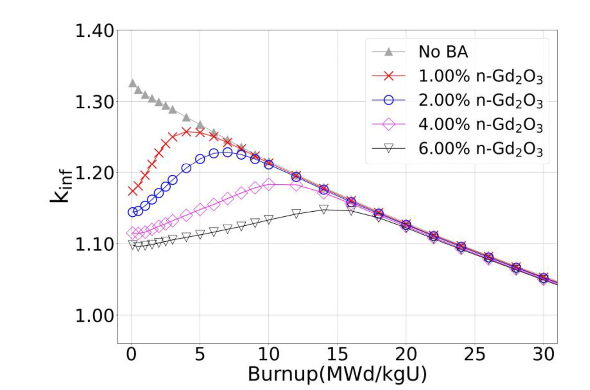
\includegraphics[width=0.78\linewidth]{images/lr_gd_kinf.pdf}
  \caption[Reactivity history of gadolinia-bearing fuel]{Multiplication factor against burnup for gadolinia contents of 1.00 to 6.00\,wt\%.\newline Figure taken from~\cite{gd_enriched_2021}.}
  \label{fig:lr-gd-kinf}
\end{figure}

In the submarine cores studied by Ippolito, this peak occurs where the
reactivity added by gadolinia depletion equals the reactivity lost to
uranium depletion~\cite{ippolito_1990}. A larger gadolinia content lowers
the peak and moves it to higher burnup~\cite{gd_enriched_2021}. After
burnout, the unburned poison and the fissile material it displaced leave a burnup penalty~\cite{alam_partI_2019}, which for natural gadolinia is small,
below $0.2\%\,\Delta k$ near 45\,GWd/MTU~\cite{ba_snf_2001}.

Gadolinia is also a means of limiting the soluble boron:

\begin{itemize}
  \item The U.S.\ EPR uses integral burnable absorbers in its first core,
        the initial fuel loading with which a new plant starts operation.
        With soluble boron alone, the moderator temperature coefficient of
        that core could be positive at the beginning of life, so the
        absorbers reduce the boron concentration and keep the coefficient
        negative at power~\cite{epr_fsar_ch4}.

  \item Low-concentration gadolinia rods combined with high-concentration
        ones lowered the boron concentration early in the cycle by up to
        300\,ppm, without loss of energy capability and without a peaking
        penalty~\cite{mildrum_segovia_2001}.

  \item Enriched gadolinia is the route taken by the i-SMR for
        soluble-boron-free operation~\cite{ismr_sbf_2024}.
\end{itemize}

Enriched gadolinium has also been studied for a Brazilian plant. For a
fuel assembly of Angra-2, the second nuclear power plant at Angra dos
Reis, Brazil, a parametric study enriched the $^{155}$Gd of a design with
only 1\,wt\% gadolinia. Above 40\,\% enrichment it suppressed the
reactivity better than the commercial design with 2\,wt\% gadolinia, and
its peak pin power stayed close to that design. The authors concluded
that enriched gadolinium is the more effective burnable absorber,
because a smaller gadolinia fraction is needed~\cite{angra2_gd_2018}.

The absorber finally moves the power peak. The rods that contain
gadolinia do not become the peak power rods, but the UO$_2$ rods of the
assemblies that carry them can~\cite{robinson_gd10}. Gadolinia rods
placed next to each other suppress their own power strongly, which
raises the power of the neighbouring UO$_2$ rods and the pin peaking
factor~\cite{radaideh_2021_rl}. Operating experience covers high
concentrations, with about 550 rods at 8\,wt\% and 32 rods at 10\,wt\%
gadolinia irradiated in pressurised water reactors by November
1986~\cite{robinson_gd10}.


% =====================================================================
%  background.tex  --  Chapter 3 (Theoretical Background)
%
%  REVISION NOTE (this version):
%   1. This chapter is the HOME OF THE FORMAL DEFINITIONS of every
%      quantity that appears in more than one chapter: F_dH
%      (eq:fdh_definition), the burnup-to-EFPD conversion (eq:efpd),
%      reactivity (eq:reactivity) and Spearman's coefficient
%      (eq:spearman). The introduction describes them qualitatively and
%      points here. The methodology defines only its own constructs
%      (estimator, end-of-cycle criterion, k_target, constraints).
%   2. Every displayed formula is followed by a term-by-term list with
%      units.
%   3. Enumerations are set as lists. No semicolons, no em dashes.
%   4. Spearman's coefficient is written rho_S to avoid the collision
%      with reactivity rho.
%   5. Cross-references into the results chapter now point to the
%      existing labels sec:res-c1c2 and sec:res-corevalidation. The
%      variable-importance subsection still does not exist and remains
%      flagged.
%
%   6. Sections 3.7-3.9 restructured into ONE section, "The dual
%      optimisation process" (label sec:bg-moo kept), with subsections
%      hypervolume (sec:bg-hv), NSGA-II (sec:bg-nsga2), GP surrogates
%      (sec:bg-gp kept) and active-learning loop (sec:bg-al kept).
%      Each subsection: step-by-step theory with book citations, then
%      an "In this thesis" paragraph tying the theory to the concrete
%      parameters of the campaigns. Traditional-book citations added
%      to Sections 3.1-3.6. New entries in references_additions.bib.
%
%   7. 14 September 2026: split into short paragraphs for human
%      reading, every enumeration set as a LaTeX list. The cost of one
%      OpenMC evaluation in Section 3.7 now reads fifteen to
%      twenty-five minutes, as in the paragraph that follows it.
%
%   8. 15 September 2026: k balance, four- and six-factor formulas
%      (Duderstadt and Hamilton) in Section 3.1. The Bateman equations
%      moved here from the literature review, with power normalisation,
%      CE and CE/CM integration and CRAM after Romano et al. 2021 and
%      Pusa 2016 (sec:bg-bateman and following). Monte Carlo section
%      split into source iteration, tallies and estimators, and
%      statistics, with formulas from Lux and Koblinger and OpenMC
%      practice from Romano et al. 2015.
%
%  Figures: the eight ORIGINAL bg_*.pdf files (generated by
%  theoretical_background_figures.py). Requires graphicx, booktabs,
%  amsmath.
% =====================================================================

\providecommand{\openpoint}[1]{\par\noindent\fbox{\parbox{0.97\linewidth}{%
  \textbf{Open point:} #1}}\par}

\chapter{Theoretical Background}
\label{ch:background}

This chapter assembles the minimum theory the thesis rests on. The
equations are stated with the source in which each is derived, and the
derivations are not repeated. The emphasis falls on the points where
theory shapes decisions taken later.

The material is ordered as the methodology uses it:

\begin{enumerate}
  \item Neutron multiplication and its leakage hierarchy.
  \item Fuel depletion and the role of the burnable absorber.
  \item The power-peaking figure of merit.
  \item The Monte Carlo method and its statistical consequences.
  \item Reduced-order proxies and rank fidelity.
  \item The dual optimisation process, built from four components:
  \begin{enumerate}
    \item the hypervolume indicator,
    \item the NSGA-II search,
    \item the Gaussian-process surrogates, and
    \item the active-learning loop.
  \end{enumerate}
\end{enumerate}

This chapter also hosts the formal definitions of the quantities used
throughout the thesis. The choices that turn those definitions into
computable numbers are methodological and are fixed in
Chapter~\ref{ch:methodology}:

\begin{itemize}
  \item The estimator.
  \item The evaluation domain.
  \item The end-of-cycle criterion.
\end{itemize}

\section{Neutron multiplication, leakage and reactivity}
\label{sec:bg-k}

The multiplication factor is the ratio of the neutron populations in
successive fission generations. A more practical definition follows from
the neutron balance of the system~\cite{duderstadt_hamilton_1976}.

\begin{equation}
k = \frac{\text{rate of neutron production}}
         {\text{rate of neutron absorption} + \text{rate of neutron leakage}}
\label{eq:k-balance}
\end{equation}

\noindent where the symbols have the following meaning:

\begin{itemize}
  \item $k$ is the multiplication factor, dimensionless.

  \item The production rate is the rate at which fission releases
        neutrons in the system, in neutrons\,s$^{-1}$.

  \item The absorption and leakage rates are the rates at which neutrons
        are absorbed in the system and escape from it, in
        neutrons\,s$^{-1}$.
\end{itemize}

In an infinite system no neutron escapes, and the non-leakage
probability is one. For a thermal reactor the neutron life cycle then
splits the multiplication factor into four factors, known as the
four-factor formula~\cite{duderstadt_hamilton_1976}.

\begin{equation}
k_\infty = \eta\, f\, p\, \varepsilon
\label{eq:kinf}
\end{equation}

\noindent where the symbols have the following meaning:

\begin{itemize}
  \item $k_\infty$ is the infinite multiplication factor, dimensionless.

  \item $\eta$ is the thermal fission reproduction factor, the number of
        fission neutrons produced per thermal neutron absorbed in the
        fuel, dimensionless.

  \item $f$ is the thermal utilisation, the probability that an absorbed
        thermal neutron is absorbed in the fuel, dimensionless.

  \item $p$ is the resonance escape probability, the probability that a
        fast fission neutron slows down to thermal energies without being
        captured, notably in the resonances of $^{238}$U, dimensionless.

  \item $\varepsilon$ is the fast fission factor, the ratio of the fast
        neutrons produced by fast and thermal fission to those produced
        by thermal fission alone, dimensionless.
\end{itemize}

In a finite system some neutrons leak out while they slow down and some
after they have reached thermal energies. Each loss enters as a
non-leakage probability, which gives the six-factor formula for the
effective multiplication factor~\cite{duderstadt_hamilton_1976}.

\begin{equation}
k_\mathrm{eff} = k_\infty\, P_\mathrm{FNL}\, P_\mathrm{TNL}
= \eta\, f\, p\, \varepsilon\, P_\mathrm{FNL}\, P_\mathrm{TNL}
\label{eq:keff}
\end{equation}

\noindent where the symbols have the following meaning:

\begin{itemize}
  \item $k_\mathrm{eff}$ is the effective multiplication factor of the
        finite system, dimensionless.

  \item $P_\mathrm{FNL}$ is the fast non-leakage probability, the
        probability that a fast neutron does not leak out of the system,
        dimensionless.

  \item $P_\mathrm{TNL}$ is the thermal non-leakage probability, the
        probability that a thermal neutron does not leak out of the
        system, dimensionless.
\end{itemize}

Both probabilities are below one in a finite system, so $k_\mathrm{eff}$
is always smaller than $k_\infty$ for the same material composition. The
factors give a physical reading of the multiplication factor. In this
work $k$ itself is estimated directly by OpenMC from continuous-energy
transport over successive fission generations, as described in
Section~\ref{sec:bg-mc-k}.

Figure~\ref{fig:bg-k} shows this hierarchy measured on C9-47, one of the
designs of the Campaign 9 Pareto set, at beginning of life with all rods
out and the fixed soluble boron concentration of the campaign model. The
three-dimensional value falls below unity because that concentration
exceeds the critical one for this design, which is treated in
Section~\ref{sec:meth-boron}.

Each geometric step opens an additional leakage path. The
ratio of the core value to the assembly value defines the
leakage-corrected end-of-cycle target used throughout the optimisation:

\begin{itemize}
  \item Single assembly under reflective boundaries,
        $k_\infty = 1.11414 \pm 0.00071$, dimensionless, from two seeds
        of \num{10000} particles and 120 batches with 30 inactive.

  \item Two-dimensional core of 32 assemblies with reflector and vacuum
        outer boundary, $k_\mathrm{eff} = 1.02742 \pm 0.00015$,
        dimensionless, from two seeds of \num{150000} particles and 200
        batches with 80 inactive. The step of \SI{-7575}{pcm} measures
        the radial leakage of the finite core.

  \item Three-dimensional core of finite height with its structural
        components, namely the nozzles, end caps, plenum springs, spacer
        grids, control-rod stack, barrel, downcomer and vessel wall,
        $k_\mathrm{eff} = 0.99690 \pm 0.00015$, dimensionless, at the
        same fidelity. The further step is \SI{-2980}{pcm}.
\end{itemize}

\begin{figure}[htbp]
  \centering
  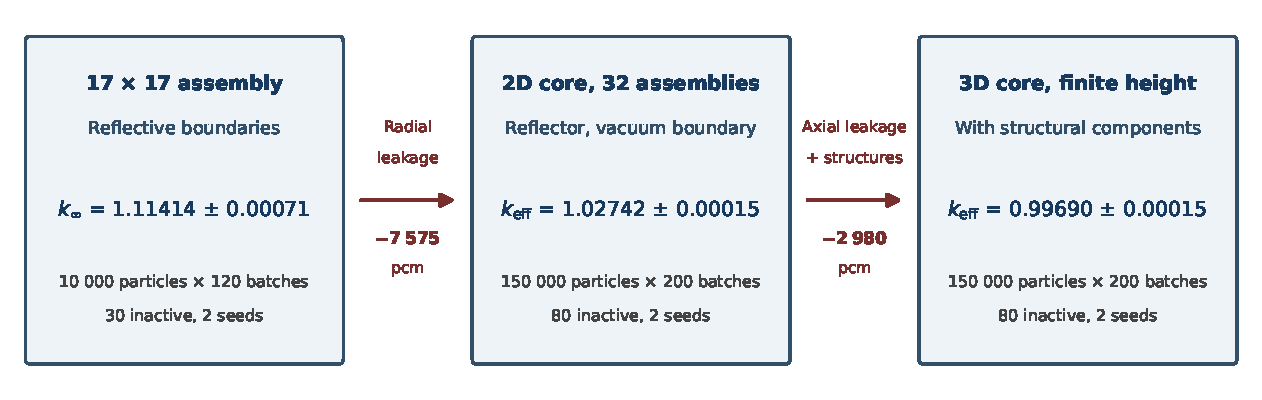
\includegraphics[width=0.92\linewidth]{images/bg_k_hierarchy.pdf}
  \caption{Multiplication ladder of C9-47, a design of the Campaign 9 Pareto set.}
  \label{fig:bg-k}
\end{figure}

Reactivity expresses the departure from criticality in a form that adds
linearly for small perturbations.

\begin{equation}
\rho = \frac{k - 1}{k}
\label{eq:reactivity}
\end{equation}

\noindent where the symbols have the following meaning:

\begin{itemize}
  \item $\rho$ is the reactivity, dimensionless, commonly reported in
        per cent mille (pcm), where $1~\mathrm{pcm} = 10^{-5}$.

  \item $k$ is the multiplication factor of the system under
        consideration, either $k_\infty$ or $k_\mathrm{eff}$,
        dimensionless.
\end{itemize}

Two competing requirements act on the beginning-of-life (BOL)
multiplication factor:

\begin{enumerate}
  \item It must exceed unity by enough margin that the core stays
        critical through the intended depletion history.

  \item It must remain bounded above, so that the excess reactivity can
        be held down by the available burnable absorber and control-rod
        worth.
\end{enumerate}

Both requirements enter the optimisation as explicit inequality
constraints on $k_\mathrm{BOL}$. The numerical bounds and their
evaluation level are given in Table~\ref{tab:constraints}.

A further consequence follows from the model level chosen for the
depletion. Because the depletion calculation is performed on the
\emph{assembly} under reflective boundaries, end of cycle cannot be
defined at $k_\infty = 1$.

The finite core that the assembly represents loses reactivity to
leakage, so the end-of-cycle criterion must be raised above unity by a
leakage correction. That correction is the target multiplication factor
formally defined in Section~\ref{sec:meth-ktarget}.

\section{Depletion, burnup and cycle length}
\label{sec:bg-depletion}

As fissile material is consumed and absorbing fission products
accumulate, the multiplication factor falls with burnup.

Burnup is the thermal energy released per unit mass of heavy metal
initially present, expressed in MWd/kgHM. It is the natural independent
variable of a depletion calculation because it is independent of the
power level at which the energy was produced.

The isotopic evolution obeys coupled rate equations of production,
decay and absorption for every nuclide~\cite{duderstadt_hamilton_1976},
known as the Bateman equations. They are solved here by the OpenMC
depletion module, with reaction rates updated by transport solutions on
an adaptive burnup schedule. The equations and the method of solution
are given in Section~\ref{sec:bg-bateman}.

The depletion runs at constant power, normalised to the heavy-metal
mass loaded at beginning of life, and burnup is referred to that same
initial mass. The specific power $P_\mathrm{spec}$ is therefore constant
by construction, and burnup grows linearly with irradiation time,
$B = P_\mathrm{spec}\,t/10^{3}$ with $t$ in days~\cite{lee_2020}.
Cycle length is
therefore reported in effective full-power days (EFPD), obtained from
the end-of-cycle burnup through the conversion below.

\begin{equation}
\mathrm{EFPD} = \frac{10^{3}\,B_\mathrm{EOC}}{P_\mathrm{spec}}
\label{eq:efpd}
\end{equation}

\noindent where the symbols have the following meaning:

\begin{itemize}
  \item $\mathrm{EFPD}$ is the cycle length in effective full-power
        days, in days.

  \item $B_\mathrm{EOC}$ is the end-of-cycle burnup, in MWd/kgHM.

  \item $P_\mathrm{spec}$ is the specific power of the fuel, in
        W\,g$^{-1}$ of heavy metal, numerically equal to
        kW\,kg$^{-1}$ of heavy metal.

  \item $10^{3}$ converts megawatt-days into kilowatt-days, so that the
        ratio closes to days.
\end{itemize}

The numerator is strictly the burnup increment accumulated over the
cycle, $B_\mathrm{EOC} - B_\mathrm{BOC}$. It reduces to
$B_\mathrm{EOC}$ here because the core is a fresh, uniform,
single-batch loading, so the beginning-of-cycle burnup is zero. A
multi-batch core would require the increment in its place.

The criterion that fixes the end-of-cycle burnup $B_\mathrm{EOC}$ is a
methodological choice. The criterion used in this work, together with
the treatment of the discharge-burnup limit, is defined in
Section~\ref{sec:objective_functions}.

Figure~\ref{fig:bg-dep} illustrates how $k_\infty$ of an assembly
evolves with burnup, using three designs of this work that differ in
enrichment and gadolinia loading. Three features of such curves matter
for the optimisation:

\begin{enumerate}
  \item The reactivity-defined end of cycle, reached where $k_\infty$
        crosses the leakage-corrected target of
        Section~\ref{sec:meth-ktarget}. A higher enrichment moves the
        crossing to a higher burnup and lengthens the cycle.

  \item The gadolinia hold-down and its burnout. A large gadolinia load
        holds $k_\infty$ down at the start of life, and its burnout then
        raises $k_\infty$ to a peak before fuel depletion takes over. A
        small load leaves no visible rise, and $k_\infty$ falls
        throughout the cycle after the initial xenon drop.

  \item The discharge-burnup limit of the fuel, which ends irradiation
        whenever the reactivity crossing lies beyond it, so the cycle
        length of a highly enriched design is set by the limit instead
        of by reactivity. The curves are assembly-average burnup, so the
        figure marks the assembly-average limit of \SI{55}{MWd/kgHM} of
        uranium dioxide in zirconium cladding~\cite{song_sanchez_2026}.
        The limit adopted for the accident-tolerant fuel of this work is
        defined in Section~\ref{sec:meth-atf}.
\end{enumerate}

\begin{figure}[htbp]
  \centering
  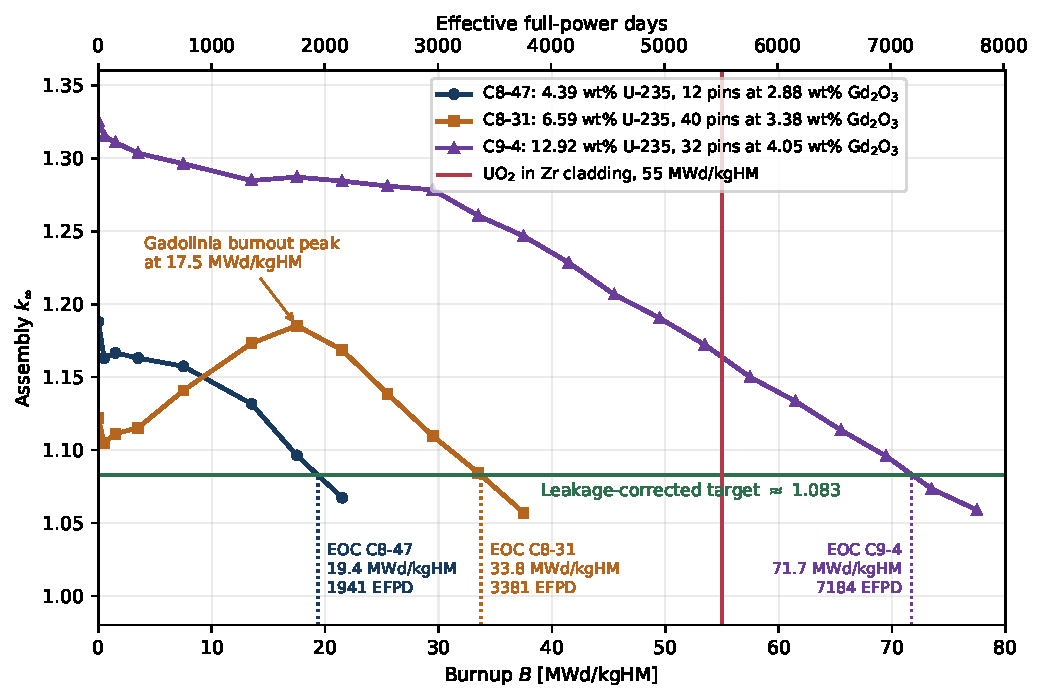
\includegraphics[width=0.9\linewidth]{images/bg_gd_depletion.pdf}
  \caption{Assembly life curves of designs C8-47, C8-31 and C9-4.}
  \label{fig:bg-dep}
\end{figure}

\subsection{The depletion equations}
\label{sec:bg-bateman}

The depletion calculations of this work follow the formulation of the
OpenMC depletion module~\cite{romano_2021_depletion}. The density of
each nuclide rises through production from other nuclides, by
transmutation and by decay, and falls through its own transmutation and
decay. Written for every nuclide, this balance gives the Bateman
equations~\cite{romano_2021_depletion}.

\begin{equation}
\begin{split}
\frac{\mathrm{d}N_i(t)}{\mathrm{d}t} = {} &
\sum_{j=1}^{n}\left[\int_0^\infty \mathrm{d}E\,
f_{j\rightarrow i}(E)\,\sigma_j(E,t)\,\phi(E,t)
+ \lambda_{j\rightarrow i}\right] N_j(t) \\
& - \left[\int_0^\infty \mathrm{d}E\,\sigma_i(E,t)\,\phi(E,t)
+ \sum_{j=1}^{n}\lambda_{i\rightarrow j}\right] N_i(t),
\qquad i = 1,\dots,n
\end{split}
\label{eq:bateman}
\end{equation}

\noindent where the symbols have the following meaning:

\begin{itemize}
  \item $N_i(t)$ and $N_j(t)$ are the densities of nuclides $i$ and $j$
        at time $t$, in atoms\,cm$^{-3}$.

  \item $t$ is the time, in s.

  \item $E$ is the neutron energy, in eV.

  \item $\phi(E,t)$ is the neutron flux at energy $E$ and time $t$, in
        cm$^{-2}$\,s$^{-1}$\,eV$^{-1}$.

  \item $\sigma_i(E,t)$ is the transmutation cross section of nuclide
        $i$, the sum of the cross sections of all reaction channels that
        transmute it, in cm$^{2}$.

  \item $f_{j\rightarrow i}(E)$ is the fraction of the transmutation
        reactions of nuclide $j$ that produce nuclide $i$,
        dimensionless.

  \item $\lambda_{j\rightarrow i}$ is the decay constant of the decay
        modes of nuclide $j$ that produce nuclide $i$, in s$^{-1}$.

  \item $n$ is the total number of nuclides, dimensionless.
\end{itemize}

By definition $f_{i\rightarrow i}$ and $\lambda_{i\rightarrow i}$ are
zero, so the sums run over all nuclides except $i$. The initial
densities $N_i(0) = N_{i,0}$ close the system. Collecting the $n$
densities into one vector gives the matrix
form~\cite{romano_2021_depletion}.

\begin{equation}
\frac{\mathrm{d}\mathbf{n}}{\mathrm{d}t} =
\mathbf{A}(\mathbf{n})\,\mathbf{n},
\qquad \mathbf{n}(0) = \mathbf{n}_0
\label{eq:bateman-matrix}
\end{equation}

\noindent where the symbols have the following meaning:

\begin{itemize}
  \item $\mathbf{n}$ is the vector of nuclide densities, with components
        in atoms\,cm$^{-3}$, and $\mathbf{n}_0$ is its initial value.

  \item $\mathbf{A}(\mathbf{n})$ is the burnup matrix, whose entries are
        the bracketed coefficients of Equation~\eqref{eq:bateman}, in
        s$^{-1}$.
\end{itemize}

The matrix depends on the composition. Evaluating $\mathbf{A}$ for a
given composition amounts to solving the neutron transport equation for
the transmutation reaction rates and combining them with decay and
fission product yield data~\cite{romano_2021_depletion}. The system is
therefore nonlinear, and every evaluation of the matrix costs one
transport solution.

\subsection{Reaction rates and power normalisation}
\label{sec:bg-dep-norm}

OpenMC obtains the reaction rates of Equation~\eqref{eq:bateman} by
tallying them directly in each depleted material. A tally can be scored
with an analog, a collision or a track-length estimator
(Section~\ref{sec:bg-mc-tally}). The depletion module does not set an
estimator on its reaction-rate tally, which carries only material
filters and reaction scores, so OpenMC applies its default track-length
estimator~\cite{romano_2021_depletion,openmc_docs}. The tallied rates are expressed in reactions per source particle, while
the depletion needs absolute rates in reactions per second.

The conversion uses the total heating observed in the system. The ratio
of the system power to the observed heating is applied as a
normalisation factor to every reaction
rate~\cite{romano_2021_depletion}.

\begin{equation}
R_{i,x} = \frac{P}{H}\,\hat{R}_{i,x}
\label{eq:dep-norm}
\end{equation}

\noindent where the symbols have the following meaning:

\begin{itemize}
  \item $R_{i,x}$ is the absolute rate of reaction $x$ in nuclide $i$,
        in reactions\,s$^{-1}$.

  \item $\hat{R}_{i,x}$ is the tallied rate of the same reaction, in
        reactions per source particle.

  \item $P$ is the system power, in W. In this work it is the product of
        the specific power $P_\mathrm{spec}$ of Equation~\eqref{eq:efpd}
        and the fresh heavy-metal mass of the model, held constant
        through the cycle.

  \item $H$ is the heating observed in the system, in J per source
        particle.
\end{itemize}

The observed heating can be determined in two
ways~\cite{romano_2021_depletion}:

\begin{enumerate}
  \item From the fission reaction rates, each multiplied by a constant
        energy release per fission (Q value) taken from the depletion
        chain file.

  \item From a tally of the actual heating rate over the whole system.
\end{enumerate}

The depletion operator of this work leaves the normalisation mode at the
default of the OpenMC coupled operator, which is the first option. The
energy released per fission therefore enters every depletion through the
Q values of the chain file.

\subsection{Integration over a time step}
\label{sec:bg-dep-integ}

For a matrix held constant, Equation~\eqref{eq:bateman-matrix} has an
exact solution in the form of a matrix
exponential~\cite{romano_2021_depletion}.

\begin{equation}
\mathbf{n}(t) = \exp(\mathbf{A}t)\,\mathbf{n}_0,
\qquad
\exp(\mathbf{X}) = \sum_{m=0}^{\infty}\frac{\mathbf{X}^{m}}{m!}
\label{eq:mat-exp}
\end{equation}

\noindent where the symbols have the following meaning:

\begin{itemize}
  \item $\exp(\cdot)$ is the matrix exponential.

  \item $\mathbf{X}$ is a square matrix, with $\mathbf{X}^{0}$ equal to
        the identity matrix $\mathbf{I}$.

  \item $m$ is the summation index, dimensionless.
\end{itemize}

Since the matrix depends on the composition, the exponential is applied
step by step with an approximation of the matrix over each step. The
simplest numerical method, constant extrapolation (CE), holds the matrix
constant over the step at its value at the start of the
step~\cite{romano_2021_depletion}.

\begin{equation}
\mathbf{n}_{i+1} = \exp\!\big(h\,\mathbf{A}(\mathbf{n}_i)\big)\,\mathbf{n}_i
\label{eq:dep-ce}
\end{equation}

\noindent where the symbols have the following meaning:

\begin{itemize}
  \item $\mathbf{n}_i$ and $\mathbf{n}_{i+1}$ are the compositions at
        the start and at the end of step $i$, in atoms\,cm$^{-3}$. Here
        the index $i$ counts time steps, not nuclides.

  \item $h$ is the length of the step, in s.
\end{itemize}

The CE method needs a single transport solution and a single matrix
exponential per step, and it is only first-order accurate, with an error
that converges as $\mathcal{O}(h)$~\cite{romano_2021_depletion}. It is
the scheme of the \texttt{PredictorIntegrator} class of OpenMC, which
every depletion of this work uses. Its accuracy is therefore governed by
the length of the steps, which the burnup schedule of
Chapter~\ref{ch:methodology} fixes.

Higher accuracy is obtained by evaluating the matrix again inside the
step. The constant extrapolation, constant midpoint (CE/CM) method first
advances the composition to the middle of the step and then uses the
matrix at the midpoint over the whole step~\cite{romano_2021_depletion}.

\begin{equation}
\begin{aligned}
\mathbf{n}_{i+1/2} &= \exp\!\left(\tfrac{h}{2}\,\mathbf{A}(\mathbf{n}_i)\right)\mathbf{n}_i \\
\mathbf{n}_{i+1} &= \exp\!\big(h\,\mathbf{A}(\mathbf{n}_{i+1/2})\big)\,\mathbf{n}_i
\end{aligned}
\label{eq:dep-cecm}
\end{equation}

\noindent where $\mathbf{n}_{i+1/2}$ is the composition at the middle of
step $i$, in atoms\,cm$^{-3}$. The CE/CM method requires two transport
solutions and two matrix exponentials per step, twice the cost of the CE
method, and it is second-order accurate~\cite{romano_2021_depletion}.

The OpenMC depletion module offers further schemes of the same
family~\cite{romano_2021_depletion}:

\begin{itemize}
  \item Constant extrapolation with linear interpolation (CE/LI) and
        linear extrapolation with quadratic interpolation (LE/QI), which
        interpolate the matrix between the start and the end of the
        step.

  \item The fourth-order Lie group integrator CF4, with four transport
        solutions per step, which allows long steps without loss of
        accuracy.

  \item The classic fourth-order Runge--Kutta method written in
        exponential form.

  \item Stochastic implicit versions of the CE, CE/LI and LE/QI methods.
\end{itemize}

All the explicit schemes are only conditionally stable, and oscillating
and diverging solutions have been observed with them. The stochastic
implicit method of Dufek et al.\ is unconditionally stable but, like the
CE method, only first-order accurate~\cite{romano_2021_depletion}. The
consequences of this instability for Monte Carlo depletion are discussed
in Section~\ref{sec:lit-opt-burnup}.

\subsection{The matrix exponential by CRAM}
\label{sec:bg-dep-cram}

Every scheme above needs the exponential of a burnup matrix, and burnup
matrices are hard for general-purpose methods. The decay constants vary
so widely that the short-lived nuclides produce eigenvalues with
absolute values up to the order of $10^{21}$, and depletion steps range
from a few days to several months. Methods built on an approximation
near the origin, such as the truncated Taylor series or the Pad\'e
approximation, work well only when the norm of $\mathbf{A}t$ is small,
which is not the case for burnup matrices~\cite{pusa_2016}.

The Chebyshev rational approximation method (CRAM) replaces the
exponential with its best rational approximation on the negative real
axis~\cite{pusa_2016}. OpenMC evaluates it in the incomplete partial
fraction form~\cite{romano_2021_depletion}.

\begin{equation}
\exp(\mathbf{A}t) \approx \alpha_0 \prod_{l=1}^{q/2}
\left(\mathbf{I} + 2\,\mathrm{Re}\!\left[\tilde{\alpha}_l\,
(\mathbf{A}t - \theta_l\mathbf{I})^{-1}\right]\right)
\label{eq:cram}
\end{equation}

\noindent where the symbols have the following meaning:

\begin{itemize}
  \item $q$ is the order of the approximation, an even number,
        dimensionless.

  \item $\alpha_0$ is the limit of the rational approximation at
        infinity, dimensionless.

  \item $\theta_l$ are the poles of the approximation, complex and
        dimensionless.

  \item $\tilde{\alpha}_l$ are the residues of its degree-two factors,
        complex and dimensionless.

  \item $\mathrm{Re}[\cdot]$ is the real part, and $\mathbf{I}$ is the
        identity matrix.
\end{itemize}

Each factor of the product requires the solution of one sparse linear
system, so an approximation of order $q$ requires $q/2$ solutions.
OpenMC uses order 48 by default, which means 24 sparse linear systems for
each matrix exponential~\cite{romano_2021_depletion}. For a burnup system
of 1606 nuclides and a step of ten days, order 16 already gives maximum
relative errors of the order of $10^{-5}$, while pure decay calculations
need higher orders~\cite{pusa_2016}.

\section{Power peaking}
\label{sec:bg-peaking}

Thermal margins are governed by the power of the hottest fuel rod, and
the core average says little about them.

A thermal design margin is the allowance kept between the operating
limits and the limits at which the fuel or the cladding fails. The
thermal design limits of a pressurised water reactor are set on three
mechanisms~\cite{todreas_kazimi_2012}:

\begin{enumerate}
  \item Departure from nucleate boiling, in which the well-behaved
        bubble formation on the cladding surface gives way to a
        continuous vapour film. Because steam conducts heat poorly, the
        cladding temperature then rises by hundreds of kelvin within
        seconds. This is the governing limit in normal operation.

  \item Melting of the fuel pellet centre, which is the hottest point
        of the core.

  \item The peak cladding temperature reached during a loss-of-coolant
        accident, which depends on the energy stored in the hottest rod
        when the transient begins.
\end{enumerate}

All three are properties of the single most heavily loaded rod. A
neutronic power distribution over several hundred rods must therefore be
reduced to a figure of merit that expresses how much worse that rod is
than the mean. The radial peaking factor $F_{\Delta H}$ is the figure of
merit used in this work for that purpose.

The connection to the first mechanism is direct. The enthalpy rise of
the coolant along a channel is proportional to the total power added
along it, which is the axially integrated power of the adjacent
rod~\cite{todreas_kazimi_2012}.

A channel with a high $F_{\Delta H}$ therefore reaches the boiling
crisis at a lower core power. Flattening the radial power distribution
buys margin that can be spent on power output or on cycle length.

The radial peaking factor is defined as the ratio between the axially
integrated linear power of the most heavily loaded fuel rod and the
average axially integrated linear power of all fuel rods in the
evaluation domain.

\begin{equation}
F_{\Delta H}
=
\frac{\displaystyle \max_{i \in \{1,\dots,N\}} \int_{0}^{H} q'_i(z)\,\mathrm{d}z}
     {\displaystyle \frac{1}{N} \sum_{j=1}^{N} \int_{0}^{H} q'_j(z)\,\mathrm{d}z}
\label{eq:fdh_definition}
\end{equation}

\noindent where the symbols have the following meaning:

\begin{itemize}
  \item $F_{\Delta H}$ is the radial peaking factor, dimensionless,
        equal to unity for a perfectly flat radial power distribution.

  \item $q'_i(z)$ is the linear power density of fuel rod $i$ at axial
        elevation $z$, in W\,cm$^{-1}$.

  \item $z$ is the axial coordinate measured from the bottom of the
        active fuel region, in cm.

  \item $H$ is the active fuel height, in cm.

  \item $N$ is the number of fuel rods in the evaluation domain,
        dimensionless.

  \item $i$ and $j$ are fuel rod indices, dimensionless.
\end{itemize}

The factor is a thermal-hydraulic margin indicator expressed in purely
neutronic terms. That is what allows it to serve as an objective in a
model without thermal-hydraulic feedback.

Two methodological choices remain, and both are fixed in
Section~\ref{sec:objective_functions}:

\begin{itemize}
  \item The evaluation domain over which the maximum is taken.

  \item The Monte Carlo estimator that replaces the integrals in
        practice.
\end{itemize}

Figures~\ref{fig:bg-pin-asm} and~\ref{fig:bg-pin-core} illustrate the
radial peaking factor on C9-47, one of the designs of the Campaign 9
Pareto set, at beginning of life. Each map shows the fission rate of every pin divided by the mean
over the fuelled pins, so $F_{\Delta H}$ is the largest value of the
map.

In the assembly with reflective boundaries of
Figure~\ref{fig:bg-pin-asm}, only the lattice shapes the distribution:

\begin{itemize}
  \item The pins next to the guide tubes, grey in the figure, receive
        extra moderation and carry the highest powers.

  \item The gadolinia-bearing pins, ringed in the figure, fall to about
        one third of the mean.
\end{itemize}

\begin{figure}[htbp]
  \centering
  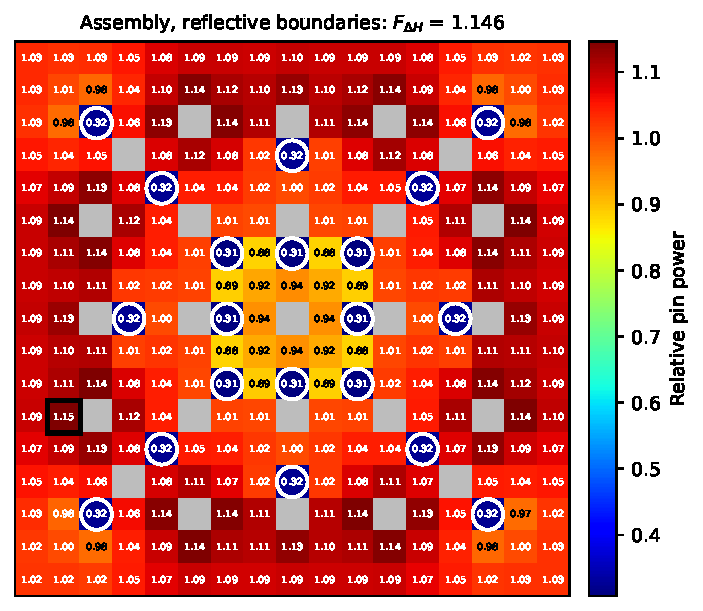
\includegraphics[width=0.60\linewidth]{images/bg_pin_power_asm.pdf}
  \caption{Relative pin power of the C9-47 assembly under reflective boundaries.}
  \label{fig:bg-pin-asm}
\end{figure}

The factor of this assembly is 1.146. In the core of
Figure~\ref{fig:bg-pin-core}, the same lattice pattern is superimposed
on the radial power shape of the finite core. Pins next to the reflector
lose neutrons to leakage, and the enrichment zoning of
Section~\ref{sec:meth-zoning} moves the peak from the centre to the
surrounding ring of assemblies, so the factor rises to 1.515. The
hottest pin is never a gadolinia-bearing pin, so a maximum-based factor
does not register the absorber directly.

\begin{figure}[htbp]
  \centering
  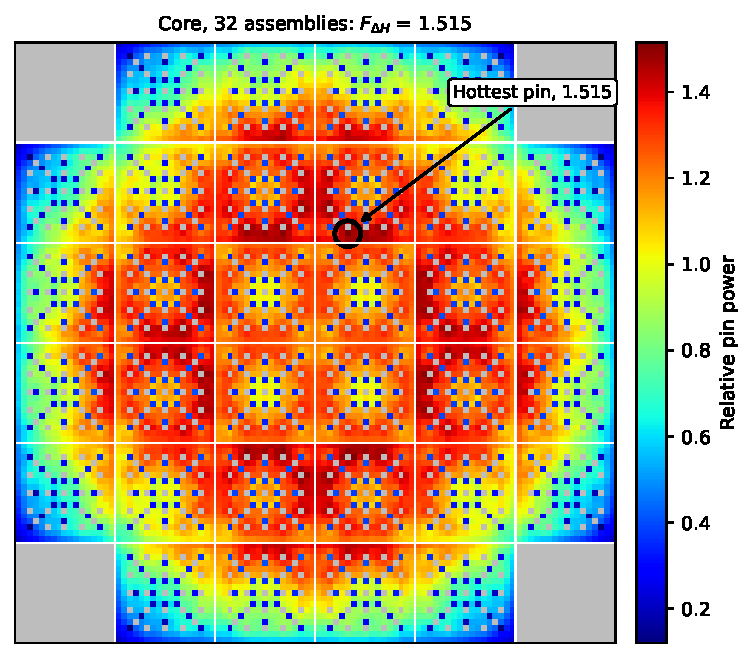
\includegraphics[width=0.64\linewidth]{images/bg_pin_power_core.pdf}
  \caption{Relative pin power of the C9-47 two-dimensional core.}
  \label{fig:bg-pin-core}
\end{figure}

Two properties of the figure of merit matter for the chapters that
follow:

\begin{enumerate}
  \item It is evaluated at beginning of life on fresh fuel, where
        enrichment zoning and absorber effects on the power
        distribution are strongest.

  \item It is a \emph{maximum over many estimated quantities}. Under
        Monte Carlo evaluation this makes it an extreme order
        statistic, with the statistical consequences developed in
        Section~\ref{sec:bg-mc}.
\end{enumerate}

\FloatBarrier

\section{Gadolinia burnable absorbers}
\label{sec:bg-gd}

Excess beginning-of-life reactivity must be held down without spending
control-rod worth~\cite{lee_2020}. Gadolinia (Gd$_2$O$_3$) mixed into
selected fuel pins achieves this
through the extreme thermal absorption of $^{155}$Gd and $^{157}$Gd.
That absorption is two to five orders of magnitude stronger than that of
the fuel nuclides, as shown in Figure~\ref{fig:bg-xs} with data from the
ENDF/B-VII.1 library used for every transport solve of this
work~\cite{chadwick_endf71_2011}.

Poisoned pellets are optically black to thermal neutrons, so absorption
proceeds from the pellet surface inward. The \emph{duration} of the
hold-down is therefore set by geometry as much as by absorber content.

Industrial practice exploits this self-shielding by concentrating the
poison in a limited number of rods~\cite{gd_enriched_2021}.

Three consequences recur in the results of this thesis:

\begin{enumerate}
  \item The number of poisoned pins sets the initial hold-down, because
        each pin absorbs from its surface, while the concentration
        within the pin sets how long the absorber
        lasts~\cite{alam_partI_2019}. The total inventory bounds the
        achievable hold-down, but the reactivity worth of the
        burnable absorber is not a function of the product of
        concentration and pin count alone.

  \item The residual end-of-life reactivity penalty of natural
        gadolinia is small~\cite{ba_snf_2001}.

  \item The local power depression couples the absorber to the peaking
        objective in a way that a maximum-based estimator cannot
        register. The absorber lowers the power of its own pin, and the
        estimator reads the hottest pin.
\end{enumerate}

\begin{figure}[htbp]
  \centering
  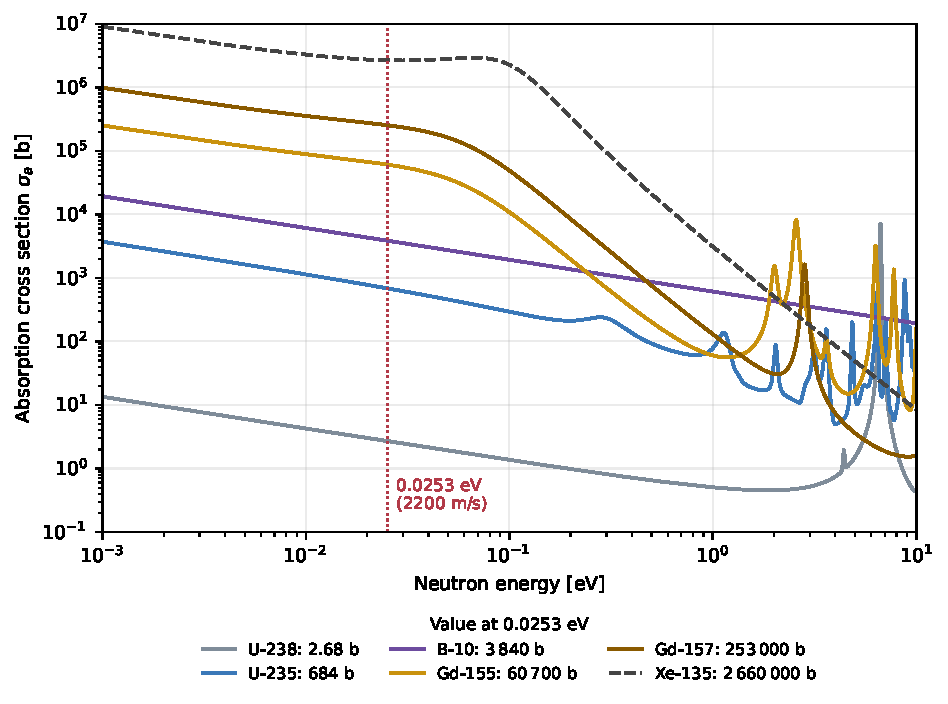
\includegraphics[width=0.8\linewidth]{images/bg_thermal_xs.pdf}
  \caption{Absorption cross sections at 294\,K from ENDF/B-VII.1.}
  \label{fig:bg-xs}
\end{figure}

\section{The Monte Carlo method and its statistics}
\label{sec:bg-mc}

OpenMC solves the transport problem by the Monte Carlo method. It follows
individual neutron histories through the geometry and scores the
quantities of interest on the events of those
histories~\cite{romano_openmc_2015}. Three parts of the method matter
for this thesis:

\begin{enumerate}
  \item The source iteration that estimates the multiplication factor
        (Section~\ref{sec:bg-mc-k}).

  \item The tallies and the estimators that score reaction rates
        (Section~\ref{sec:bg-mc-tally}).

  \item The statistics of the resulting estimates
        (Section~\ref{sec:bg-mc-stats}).
\end{enumerate}

\subsection{Source iteration and the multiplication factor}
\label{sec:bg-mc-k}

Monte Carlo estimates of the multiplication factor rest on source
iteration over successive fission generations~\cite{lux_koblinger_1991}.
OpenMC solves the $k$-eigenvalue problem by this method of successive
generations and lets several generations be grouped into a batch, which
reduces the correlation between realisations of the tally random
variables~\cite{romano_openmc_2015}. The calculation proceeds in
batches:

\begin{enumerate}
  \item A batch of neutron histories is tracked.

  \item The fission sites it produces seed the next batch.

  \item The earlier \emph{inactive} batches are discarded while the
        fission source is still settling.

  \item Tallies accumulate over the \emph{active} batches only.
\end{enumerate}

In a generation started from $N$ fission points, the estimate of the
multiplication factor is the number of fission points that the
generation produces per starting point~\cite{lux_koblinger_1991}.

\begin{equation}
\tilde{k}_g = \frac{N_g}{N}
\label{eq:mc-kn}
\end{equation}

\noindent where the symbols have the following meaning:

\begin{itemize}
  \item $\tilde{k}_g$ is the estimate of the multiplication factor in
        generation $g$, dimensionless.

  \item $N$ is the number of fission points that start each generation,
        dimensionless.

  \item $N_g$ is the number of fission points produced in generation
        $g$, dimensionless.
\end{itemize}

The first generations carry the bias of the initial source guess and are
discarded. The estimate of the multiplication factor is the average over
the remaining active generations~\cite{lux_koblinger_1991}.

\begin{equation}
\bar{k} = \frac{1}{G - G_\mathrm{in}}
\sum_{g=G_\mathrm{in}+1}^{G} \tilde{k}_g
\label{eq:mc-kbar}
\end{equation}

\noindent where the symbols have the following meaning:

\begin{itemize}
  \item $\bar{k}$ is the estimate of the multiplication factor,
        dimensionless.

  \item $G$ is the total number of generations, dimensionless.

  \item $G_\mathrm{in}$ is the number of inactive generations discarded
        at the start, dimensionless.
\end{itemize}

OpenMC keeps the collision, absorption and track-length estimators of
$k_\mathrm{eff}$ side by side and reports a minimum-variance combination
of the three, based on their covariance
matrix~\cite{romano_openmc_2015}. Source convergence is monitored
through the Shannon entropy of the fission source. A structured mesh
covering at least all the fissionable materials is superimposed on the
geometry, and the fraction of source sites in each mesh element is
counted~\cite{openmc_docs}.

\begin{equation}
H = -\sum_{i=1}^{N_\mathrm{m}} S_i \log_2 S_i,
\qquad
S_i = \frac{\text{source sites in mesh element } i}
           {\text{total number of source sites}}
\label{eq:shannon}
\end{equation}

\noindent where the symbols have the following meaning:

\begin{itemize}
  \item $H$ is the Shannon entropy of the fission source, in bits.

  \item $N_\mathrm{m}$ is the number of mesh elements, dimensionless.

  \item $S_i$ is the fraction of the source sites that lie in mesh
        element $i$, dimensionless.
\end{itemize}

The mesh of this work has 8 by 8 by 1 elements
(Appendix~\ref{app:model-inputs}). The entropy becomes stationary once
the spatial source has settled.

The entropy is recorded for every evaluation from Campaign~3 onward as a
source-convergence diagnostic. The diagnostic does not stop or repeat an
evaluation inside the loop. The core solves are instead given 60 to 120
inactive batches, and the designs whose source had not converged when
the active batches began are identified afterwards
(Sections~\ref{sec:res-corevalidation}, \ref{sec:res-c7-limits}
and~\ref{sec:res-c8-limits}).

\subsection{Tallies and estimators}
\label{sec:bg-mc-tally}

Every physical result of an OpenMC run is obtained from a tally. A tally
is defined by a combination of filters and
scores~\cite{romano_openmc_2015}:

\begin{itemize}
  \item A filter limits the events that can score to the tally, based on
        attributes of the particle such as the cell it travels in or its
        pre-collision energy.

  \item A score names the physical quantity recorded for an event that
        passes the filters, such as the flux, the fission reaction rate
        or the energy deposited by fission.
\end{itemize}

Most scores are reaction rates integrated over a region of the
geometry~\cite{lux_koblinger_1991}.

\begin{equation}
R_x = \int_V \mathrm{d}\mathbf{r} \int_0^\infty \mathrm{d}E\,
\phi(\mathbf{r},E)\,\Sigma_x(\mathbf{r},E)
\label{eq:mc-rr}
\end{equation}

\noindent where the symbols have the following meaning:

\begin{itemize}
  \item $R_x$ is the rate of reaction $x$ in the region $V$, in
        reactions\,s$^{-1}$.

  \item $V$ is the region of the geometry, in cm$^{3}$, and
        $\mathbf{r}$ is the position, in cm.

  \item $E$ is the neutron energy, in eV.

  \item $\phi(\mathbf{r},E)$ is the scalar neutron flux, in
        cm$^{-2}$\,s$^{-1}$\,eV$^{-1}$.

  \item $\Sigma_x(\mathbf{r},E)$ is the macroscopic cross section of
        reaction $x$, in cm$^{-1}$.
\end{itemize}

A Monte Carlo run estimates this integral from the histories it
simulates, and OpenMC offers three estimators for it~\cite{openmc_docs}:

\begin{itemize}
  \item The analog estimator counts the reactions that actually occur
        in the region.

  \item The collision estimator scores at every collision in the
        region, whatever reaction takes place.

  \item The track-length estimator scores along every flight segment
        of the particle inside the region.
\end{itemize}

The collision estimator scores more events than the analog estimator,
each with a smaller contribution~\cite{openmc_docs}. At every collision
inside the region it scores the ratio of the reaction cross section to
the total cross section at the collision point~\cite{lux_koblinger_1991}.

\begin{equation}
\bar{R}_x^\mathrm{col} = \frac{1}{N_h} \sum_{c=1}^{n_c} w_c\,
h_V(\mathbf{r}_c)\,
\frac{\Sigma_x(\mathbf{r}_c,E_c)}{\Sigma_t(\mathbf{r}_c,E_c)}
\label{eq:mc-col}
\end{equation}

\noindent where the symbols have the following meaning:

\begin{itemize}
  \item $\bar{R}_x^\mathrm{col}$ is the collision estimate of the
        reaction rate, in reactions per source particle.

  \item $N_h$ is the number of simulated histories, dimensionless, and
        $n_c$ is the number of collisions in all of them, dimensionless.

  \item $w_c$ is the statistical weight of the particle entering
        collision $c$, dimensionless.

  \item $\mathbf{r}_c$ and $E_c$ are the position, in cm, and the energy,
        in eV, of the particle entering collision $c$.

  \item $h_V(\mathbf{r}_c)$ equals one when $\mathbf{r}_c$ lies in the
        region $V$ and zero otherwise, dimensionless.

  \item $\Sigma_t$ is the total macroscopic cross section, in cm$^{-1}$.
\end{itemize}

The track-length estimator scores along every flight segment that
crosses the region, with the length of the segment inside
it~\cite{lux_koblinger_1991}.

\begin{equation}
\bar{R}_x^\mathrm{tl} = \frac{1}{N_h} \sum_{s=1}^{n_s} w_s\, l_s\,
\Sigma_x(E_s)
\label{eq:mc-tl}
\end{equation}

\noindent where the symbols have the following meaning:

\begin{itemize}
  \item $\bar{R}_x^\mathrm{tl}$ is the track-length estimate of the
        reaction rate, in reactions per source particle.

  \item $n_s$ is the number of flight segments in all histories,
        dimensionless.

  \item $w_s$ is the statistical weight of the particle on segment $s$,
        dimensionless.

  \item $l_s$ is the length of segment $s$ inside the region $V$, in cm.

  \item $E_s$ is the energy of the particle on segment $s$, in eV, at
        which $\Sigma_x$ of the material of the region is evaluated.
\end{itemize}

The collision and track-length estimators are both unbiased estimates of the same quantity and can be evaluated
from the same set of histories~\cite{lux_koblinger_1991}. OpenMC writes
the two estimators in the same form, normalised by the total starting
weight of the particles in place of the number of
histories~\cite{openmc_docs}.

Its tallies are scored with the
track-length estimator by default~\cite{romano_openmc_2015}. A
track-length estimator cannot serve a tally that needs the state of the
particle after a collision, so tallies with outgoing-energy filters,
scattering change-in-angle filters or scattering moments use an analog
estimator~\cite{openmc_docs}. The reaction rates
that drive the depletion of Section~\ref{sec:bg-dep-norm} are
track-length estimates, because the depletion tally sets no estimator
and the default applies~\cite{romano_2021_depletion,openmc_docs}.

\subsection{Statistics of the estimates}
\label{sec:bg-mc-stats}

The active batches of a run give repeated estimates of every tally. For
$B$ batches, the result and its uncertainty are estimated by the sample
mean and by the sample variance of the mean~\cite{lux_koblinger_1991}.

\begin{equation}
\hat{x} = \frac{1}{B}\sum_{b=1}^{B}\bar{x}_b,
\qquad
s_{\hat{x}}^2 = \frac{1}{B(B-1)}\sum_{b=1}^{B}
\left(\bar{x}_b - \hat{x}\right)^2
\label{eq:mc-mean-var}
\end{equation}

\noindent where the symbols have the following meaning:

\begin{itemize}
  \item $\hat{x}$ is the estimate of the tallied quantity, in the units
        of the tally.

  \item $\bar{x}_b$ is the estimate of the same quantity from batch $b$,
        in the units of the tally.

  \item $B$ is the number of active batches, dimensionless.

  \item $s_{\hat{x}}^2$ is the sample variance of the mean, in the
        squared units of the tally.
\end{itemize}

The expected value of this variance equals the variance of the score of
a single history divided by the total number of histories, whatever the
size of the batches~\cite{lux_koblinger_1991}.

\begin{equation}
\left\langle s_{\hat{x}}^2 \right\rangle = \frac{D^2}{N_h}
\label{eq:mc-var-exp}
\end{equation}

\noindent where the symbols have the following meaning:

\begin{itemize}
  \item $\langle\cdot\rangle$ is the expected value.

  \item $D^2$ is the variance of the score of a single history, in the
        squared units of the tally.

  \item $N_h$ is the total number of active histories, dimensionless.
\end{itemize}

The standard deviation of the mean therefore falls as $1/\sqrt{N_h}$.
These formulas assume that the batch estimates are independent.
Successive generations of an eigenvalue calculation are correlated, and
grouping generations into batches is the means OpenMC provides to reduce
that correlation~\cite{romano_openmc_2015}. OpenMC reports the mean and
the standard deviation of every tally bin, and its confidence intervals
use the Student $t$ distribution with $B-1$ degrees of
freedom~\cite{openmc_docs}.

Every tallied quantity is a statistical estimate. Two properties of
those estimates drive the methodology of this thesis, and both are
illustrated in Figure~\ref{fig:bg-mc}:

\begin{enumerate}
  \item The standard deviation of a tally contracts with the inverse
        square root of the number of active histories
        (Equation~\eqref{eq:mc-var-exp}). Panel~(a) tests this law
        on the seed-to-seed standard deviation of the assembly
        $F_{\Delta H}$, pooled over the designs re-scored with five or
        eight seeds at \num{16000}, \num{64000} and \num{256000}
        particles and 120 batches. The three points follow the law within
        their sampling error, and a fit with a free exponent gives
        $-0.48$ against the theoretical $-0.5$.

  \item An objective defined as the \emph{maximum} over many noisy
        cells is an extreme order statistic, whose distribution and
        expected value follow from those of the individual
        cells~\cite{david_nagaraja_2003}. It is biased \emph{upward},
        because the cell that wins is preferentially one that
        fluctuated high.
\end{enumerate}

The law holds for the maximum only once a single pin dominates it. At
low fidelity several pins compete for the maximum, and the estimate
inherits the narrower spread of the largest of several noisy values.
The seed replication of three Campaign~2 designs at \num{4000} particles
and 60 batches, five seeds each, gives a pooled standard deviation of
$0.015 \pm 0.003$, which is not used in the fit. The same three designs
give 0.0074 at \num{16000} particles, and scaling this value with
$1/\sqrt{N}$ predicts 0.022 at the lower fidelity. The measured spread is
therefore about \SI{30}{\percent} below the law, about twice its
standard error. The synthetic field of panel~(b) shows a shortfall of
the same sign, about \SI{20}{\percent}.

The second property is the less familiar of the two and has three
practical consequences:

\begin{enumerate}
  \item At the per-cell noise level of the Campaign~2 fidelity, the
        estimated maximum over a nearly flat field of 264 cells, the
        fuel pins of one assembly, sits far above the true maximum.
        Panel~(b) shows the mechanism with synthetic samples of a field
        whose true maximum is 1.02. The per-cell noise is the mean relative
        error of the hottest pin measured at \num{256000} particles,
        about \SI{0.3}{\percent}, and at the Campaign~2 fidelity, about
        \SI{3.6}{\percent}. The mean bias of the estimate is about
        $+0.005$ at the first level and $+0.09$ at the second.

  \item Averaging the maxima obtained with independent random seeds
        narrows the distribution of the estimate but does not shift its
        centre. The bias shrinks only when each maximum is taken over
        estimates with more histories, either from a longer run or from
        tallies pooled over several seeds.

  \item The bias grows as the true power field flattens, because more
        near-ties give more opportunities for an upward fluctuation to
        win. The estimator therefore penalises most heavily exactly the
        designs that a peaking-minimising optimiser should prefer.
\end{enumerate}

This mechanism is quantified on the real campaign in
Section~\ref{sec:res-c1c2}. It is the origin of the ranking inversion
that motivates the two-stage selection methodology of
Section~\ref{sec:meth-stats}.

\begin{figure}[htbp]
  \centering
  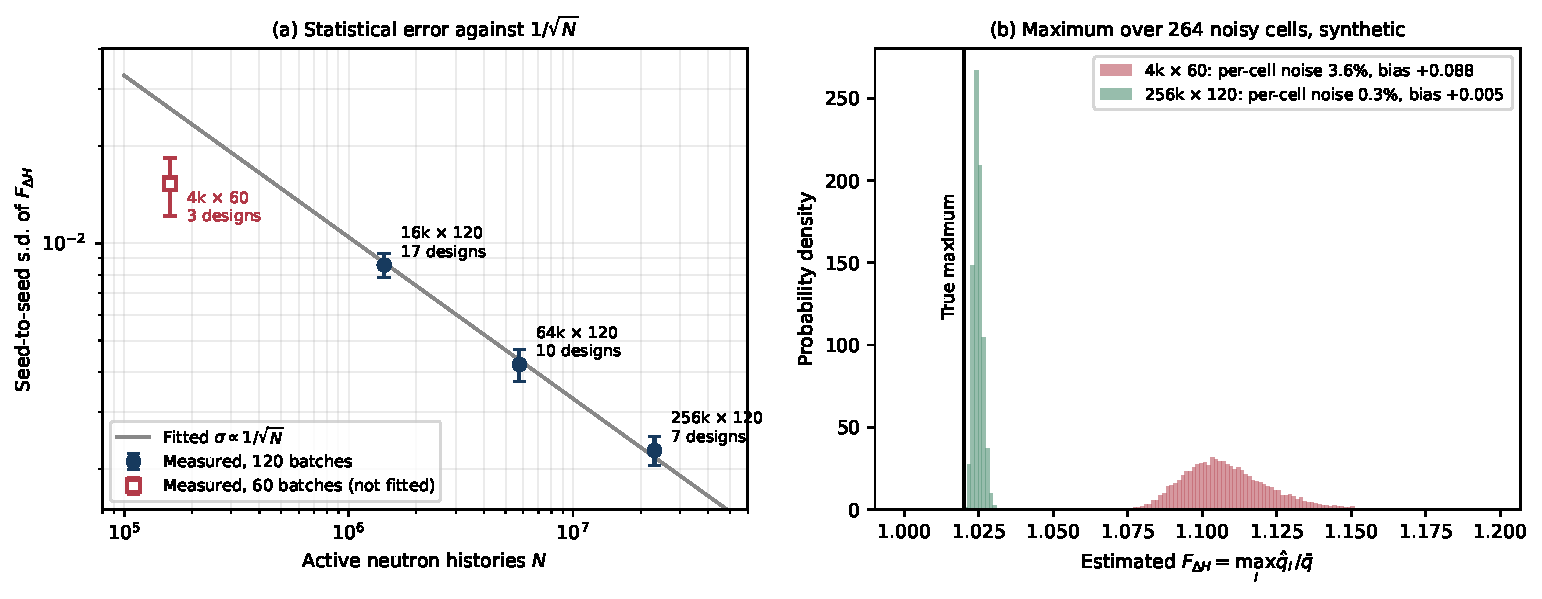
\includegraphics[width=\linewidth]{images/bg_mc_noise.pdf}
  \caption{Monte Carlo statistics of the peaking estimator.}
  \label{fig:bg-mc}
\end{figure}

\section{Reduced-order proxies and rank fidelity}
\label{sec:bg-proxy}

An optimiser driven by a cheap proxy inherits the \emph{ordering} that
the proxy imposes on candidate designs. Non-dominated sorting compares
designs pairwise, so any error that preserves the order of the designs,
such as a constant offset or scale factor, leaves the selection
unchanged. What matters for the search is therefore how well the proxy
ranks the designs, which a rank correlation measures. The absolute error
still matters wherever the proxy is compared with a fixed limit, as in a
constraint, and wherever its value is reported.

Spearman's rank correlation coefficient is used for that
purpose~\cite{kendall_gibbons_1990}. It is the Pearson correlation of
the two rankings, which for $n$ designs without tied values reduces to
Equation~\eqref{eq:spearman}.

\begin{equation}
\rho_S = 1 - \frac{6 \sum_{i=1}^{n} d_i^{\,2}}{n\,(n^{2}-1)}
\label{eq:spearman}
\end{equation}

\noindent where the symbols have the following meaning:

\begin{itemize}
  \item $\rho_S$ is Spearman's rank correlation coefficient,
        dimensionless, bounded between $-1$ and $+1$, equal to $+1$ for
        identical orderings. The subscript distinguishes it from
        reactivity, Equation~\eqref{eq:reactivity}.

  \item $d_i$ is the difference between the rank assigned to design $i$
        by the proxy and the rank assigned to the same design by the
        reference quantity, dimensionless.

  \item $n$ is the number of paired designs, dimensionless.

  \item $i$ is the design index, dimensionless.
\end{itemize}

The weakness of a rank-based proxy is systematic. Proxy-to-truth
correlation degrades near the optimum, where candidate designs crowd
together in objective space and small structural errors are enough to
reorder them.

Two responses to this problem exist in the literature, and both are
exercised in this thesis (Sections~\ref{sec:meth-core-objective}
and~\ref{sec:res-corevalidation}):

\begin{enumerate}
  \item Fuse the fidelities statistically, through a learned
        discrepancy between the cheap and the expensive
        model~\cite{kennedy_ohagan_2000,forrester_book_2008}.

  \item Measure the expensive quantity directly, wherever its cost
        permits.
\end{enumerate}

\section{The dual optimisation process}
\label{sec:bg-moo}

The optimisation of this thesis is built around a trade-off between two
costs: the cost of evaluating a design and the cost of searching for
good designs. One evaluation of the truth is a coupled OpenMC transport and depletion
calculation. It takes fifteen to twenty-five minutes, depending on the
campaign fidelity (Section~\ref{sec:meth-fidelity}).

A population-based search carries many candidate designs at once and
improves them collectively, without following a single trajectory. The
search used here, NSGA-II, is of that kind.

In Campaigns 1 to 5 NSGA-II evolved a population of 60 designs over 80
generations, which is 4800 objective evaluations for one search. From
Campaign 6 the population is 300 designs over 400 generations, or
\num{120000} evaluations. One such search is performed at every
iteration of the loop.

The change followed a sensitivity study before Campaign 6
(Section~\ref{sec:meth-nsga-setting}, Table~\ref{tab:nsga-sens}). The
surrogates were frozen on the Campaign 6 design of experiments, and
the search alone was repeated at six settings with eight seeds each:

\begin{itemize}
  \item At $60\times80$ the hypervolume of the surrogate front varied
        from seed to seed by a standard deviation of 12.7, about thirty
        per cent of the whole range covered by the six settings, so the
        selected designs depended on the seed.

  \item At $300\times400$ the hypervolume was the highest of the six and
        the seed-to-seed standard deviation fell to 0.6.

  \item The larger search costs about \SI{8}{\second}, which is
        negligible against one transport evaluation.
\end{itemize}

If each of the 4800 evaluations of the smaller search were an OpenMC
calculation, one search
alone would require seven to twelve weeks of continuous computation, and
a campaign of eight iterations between one and two years. Coupling the
search directly to the transport code is therefore computationally
prohibitive.

The resolution is a \emph{dual} process with two stages of very
different cost~\cite{forrester_book_2008}:

\begin{enumerate}
  \item An expensive \emph{evaluation} stage, in which OpenMC produces
        a small number of trusted data points.

  \item A cheap \emph{search} stage, in which a statistical model
        trained on those points is optimised in place of the code.
\end{enumerate}

Four components implement this process. The following subsections build
them in order of dependence:

\begin{enumerate}
  \item The hypervolume indicator, which measures the progress of a set
        of designs.

  \item The NSGA-II search, which produces such sets.

  \item The Gaussian-process surrogate, which makes the search
        affordable.

  \item The active-learning loop, which closes the cycle between search
        and evaluation.
\end{enumerate}

The four components share the concept of Pareto dominance, which is
defined first. With two competing objectives no single optimum exists, and the outcome of the
optimisation is a set of mutually incomparable designs.

Design $a$ \emph{dominates} design $b$ if it is at least as good as $b$
in both objectives and strictly better in at least one of
them~\cite{miettinen_1999,deb_2001}. The non-dominated subset of a design archive is its Pareto set, and the
corresponding attainment staircase in objective space is the Pareto
front, illustrated in Figure~\ref{fig:bg-pareto}.

Because the cycle length is maximised and $F_{\Delta H}$ is minimised,
the front appears there as a lower-right attainment staircase. The
reference point lies at the worst value of both objectives. Campaign~9
replaces the cycle length by the critical boron concentration
$c_\mathrm{max}$, and the cycle length becomes a constraint
(Section~\ref{sec:meth-c9}). Both objectives are then minimised, so
its front is a lower-left staircase and the reference point moves to
the upper right.

\begin{figure}[!tbp]
  \centering
  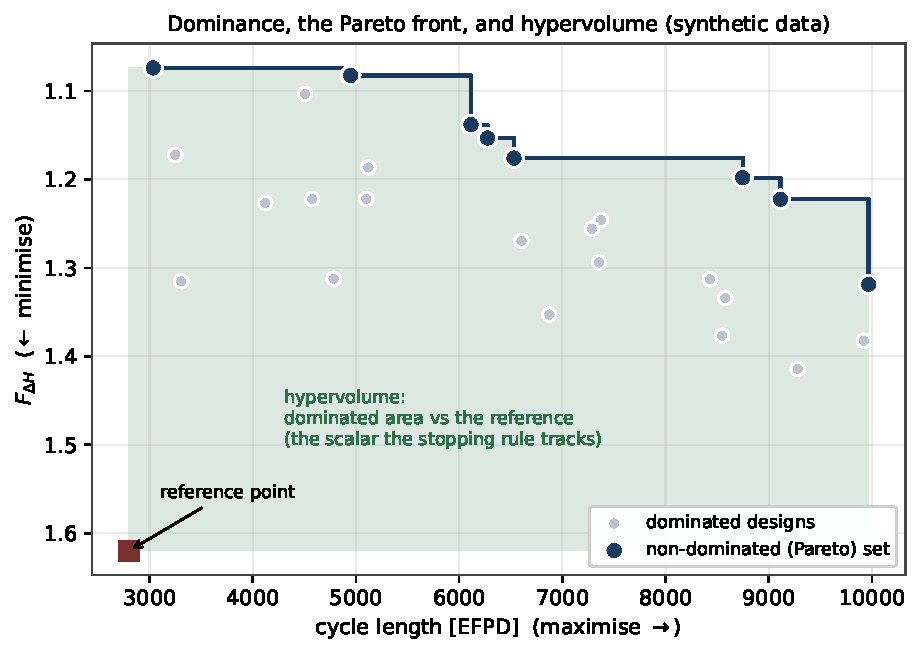
\includegraphics[width=0.82\linewidth]{images/bg_pareto_hv.pdf}
   \caption{Dominance, the Pareto front and the hypervolume.}
  \label{fig:bg-pareto}
\end{figure}

One sign convention simplifies everything that follows. Optimisation
libraries minimise by default, so the maximised objective of this
thesis, the cycle length, is negated internally and both objectives are
treated as minimisations.

All formulas below are written in that convention, and every reported
number is converted back before display.

\subsection{The hypervolume indicator}
\label{sec:bg-hv}

The search operates on \emph{sets} of designs, so its progress cannot
be tracked by watching a single number improve. The hypervolume
indicator solves this by compressing an entire Pareto front into one
scalar~\cite{coello_2007}.

\begin{equation}
\mathrm{HV}(\mathcal{P})
= \lambda\!\left( \bigcup_{\mathbf{f} \in \mathcal{P}}
  \left[\, \mathbf{f},\, \mathbf{r} \,\right] \right)
\label{eq:hv}
\end{equation}

\noindent where the symbols have the following meaning:

\begin{itemize}
  \item $\mathrm{HV}(\mathcal{P})$ is the hypervolume of the front
        $\mathcal{P}$, in the product of the objective units, for
        example EFPD times the dimensionless peaking factor in
        Campaigns 1 to 8 and the critical boron concentration, in ppm,
        times the peaking factor in Campaign~9.

  \item $\lambda$ is the Lebesgue measure, which for two objectives is
        simply the area.

  \item $\mathcal{P}$ is the set of objective vectors of the
        non-dominated designs.

  \item $\mathbf{f}$ is the objective vector of one front member, with
        one coordinate per objective.

  \item $\mathbf{r}$ is the reference point, a fixed objective vector
        chosen worse than every front member in every objective.

  \item $[\mathbf{f}, \mathbf{r}]$ is the axis-aligned rectangle
        spanned by $\mathbf{f}$ and $\mathbf{r}$, that is, the region
        of objective space dominated by that member relative to the
        reference.
\end{itemize}

Figure~\ref{fig:bg-hv-construction} illustrates the construction on a
schematic front, not on campaign data. Its four panels correspond to
the four steps below:

\begin{enumerate}
  \item Fix the reference point once, at a value worse than any design
        of interest in both objectives.

  \item For each front member, draw the rectangle between the member
        and the reference point. Everything inside that rectangle is
        dominated by the member.

  \item Take the union of the rectangles. Overlaps are counted once.

  \item The area of the union is the hypervolume.
\end{enumerate}

\begin{figure}[!tbp]
  \centering
  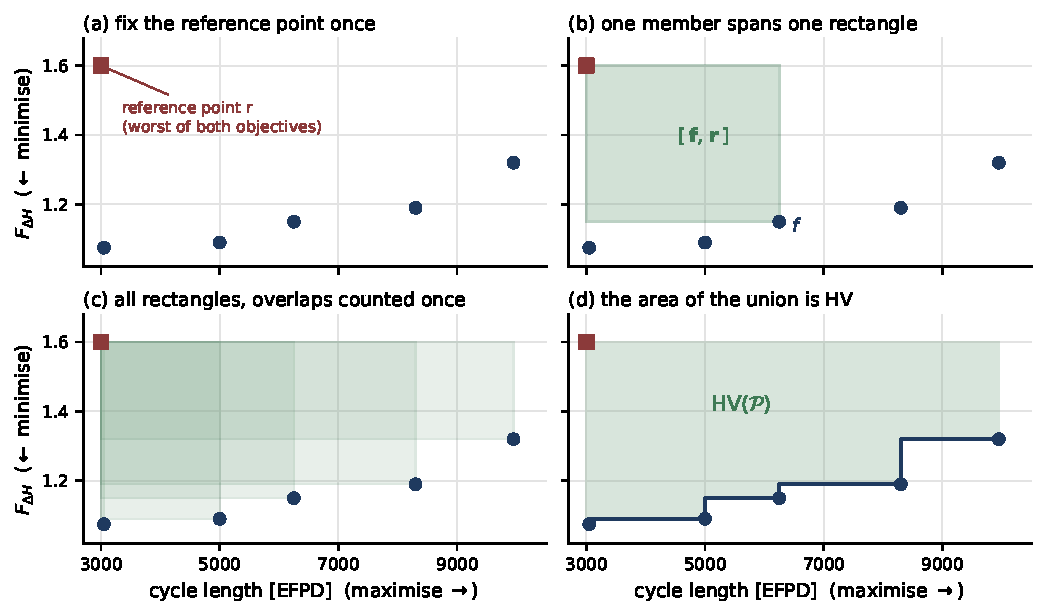
\includegraphics[width=\linewidth]{images/bg_hv_construction.pdf}
  \caption{Illustrative construction of the hypervolume.}
  \label{fig:bg-hv-construction}
\end{figure}

Two properties make the indicator the right convergence diagnostic:

\begin{enumerate}
  \item It respects Pareto dominance. When one front is better than
        another, its hypervolume is strictly larger, because the better
        front dominates a region of objective space that the other does
        not~\cite{zitzler_2003_performance}.

  \item It rewards both convergence and spread, because a front that
        covers a wider range of trade-offs dominates a larger region.
\end{enumerate}

Figure~\ref{fig:bg-hv-gain} shows the only two mechanisms by which the
indicator can grow. Of the two designs added at iteration $k+1$, one
pushes the front outward and the other fills a gap.

\begin{figure}[htbp]
  \centering
  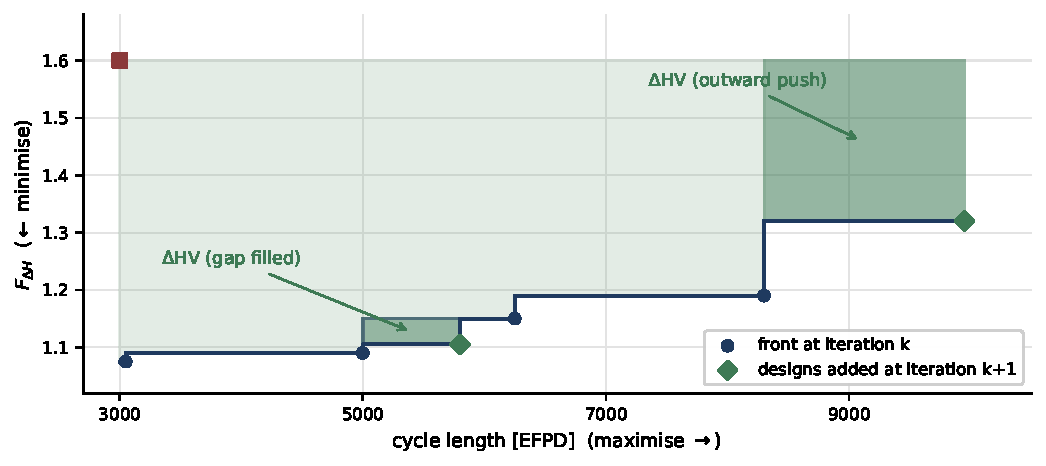
\includegraphics[width=0.9\linewidth]{images/bg_hv_gain.pdf}
  \caption{Growth of the hypervolume between two iterations.}
  \label{fig:bg-hv-gain}
\end{figure}

The indicator carries one obligation in exchange for its convenience.
Its numerical value depends on the reference point and on the units of
the objectives as much as on the front itself.

The dependence is shown below on one unchanged front measured from three
reference points. The front is the illustrative five-member front of
Figure~\ref{fig:bg-hv-construction}, not the front of any campaign, so
the values below do not appear in Chapter~\ref{ch:results}. The first
reference point is the one drawn in that figure. The other two are
alternatives that could
equally have been chosen, and are not shown:

\begin{itemize}
  \item $\mathbf{r} = (3000~\mathrm{EFPD},\, 1.60)$, the value used in
        Figure~\ref{fig:bg-hv-construction}, gives
        $\mathrm{HV} = 2886$.

  \item $\mathbf{r} = (2500~\mathrm{EFPD},\, 1.80)$, a more permissive
        corner, gives $\mathrm{HV} = 4638$.

  \item $\mathbf{r} = (3000~\mathrm{EFPD},\, 1.45)$, a stricter corner,
        gives $\mathrm{HV} = 1843$.
\end{itemize}

No design has moved between the three cases. The front is identical in
all of them, and the reported value still varies by a factor of two and
a half.

The choice of units has the same effect. The hypervolume of a
two-objective problem has the units of the product of its objectives,
for example effective full-power days multiplied by a dimensionless
factor. Reporting cycle length in years instead of days divides every
value by 365.25 without changing a single design, so an isolated
hypervolume states nothing about the quality of a front.

What carries meaning is the change in hypervolume between two
iterations, measured against the same reference point. The change is
the area of the region that the new front dominates and the previous
front did not. It is therefore positive only when a new design has moved
the front outward or filled a gap between its members, and zero when
the front is unchanged.

The stopping rule of Section~\ref{sec:meth-loop} therefore uses the gain
relative to the previous hypervolume, below \SI{1}{\percent} for three
consecutive iterations, and not an absolute value of the hypervolume. A
change of units multiplies the gain and the previous hypervolume by the
same factor, so their ratio is unchanged, while an absolute threshold
would have to be chosen again for every choice of units. The ratio still
depends on the reference point, because the reference point sets the
area credited to the extreme members of the front. The reference point
is therefore kept fixed within a campaign, as the rules below require.

Two rules of comparability follow, and both are respected throughout
this work:

\begin{enumerate}
  \item Within one campaign the reference point is fixed once and never
        revised, so every value in the history is comparable to every
        other.

  \item Across campaigns the values are not comparable whenever the
        reference point or the definition of an objective has changed,
        and no such comparison is drawn in Chapter~\ref{ch:results}.
\end{enumerate}

\subsection{The NSGA-II search}
\label{sec:bg-nsga2}

The Non-dominated Sorting Genetic Algorithm II
(NSGA-II)~\cite{deb_nsga2_2002} is the engine that produces candidate
Pareto sets. It belongs to the family of genetic algorithms, which
mimic natural selection on a population of candidate
solutions~\cite{deb_2001}.

Each design is an individual, its design vector plays the role of its
genes, and better individuals are given more descendants.

A genetic algorithm iterates four operations:

\begin{enumerate}
  \item \emph{Selection.} Better candidates are given a higher chance
        of becoming parents.

  \item \emph{Crossover.} Pairs of parents are recombined into
        offspring, the new candidate designs, whose variables combine the
        values of both parents. This work uses simulated binary
        crossover, the default operator of the NSGA-II implementation
        adopted~\cite{deb_2001,blank_deb_2020}.

  \item \emph{Mutation.} Small random perturbations keep the population
        from collapsing prematurely.

  \item \emph{Replacement.} The next generation is formed and the cycle
        repeats.
\end{enumerate}

The step that does not survive the move to two objectives is the first
one, because ``better'' is no longer a single number. A design with a
longer cycle and a design with a lower peaking factor are each better
than the other in one respect, and the same holds in Campaign~9 for a
design with a lower critical boron concentration and a design with a
lower peaking factor.

NSGA-II resolves this with two rankings computed on the current
population~\cite{deb_nsga2_2002,deb_2001}:

\begin{itemize}
  \item Non-dominated sorting, which measures quality.

  \item The crowding distance, which measures diversity.
\end{itemize}

\subsubsection*{Comparing two designs}

The basic comparison is the dominance of Section~\ref{sec:bg-moo}, and
Figure~\ref{fig:bg-nsga2-sorting}(a) shows everything it can say. Any
design $X$ splits the objective plane into four quadrants:

\begin{enumerate}
  \item Designs that are at least as good in both objectives and
        strictly better in at least one \emph{dominate} $X$, as $A$ does
        in Figure~\ref{fig:bg-nsga2-sorting}(a).

  \item Designs that are at least as bad in both, one strictly, are
        \emph{dominated by} $X$, as $B$ is.

  \item Designs in the two remaining quadrants trade one objective
        against the other. They are \emph{incomparable} with $X$, and
        dominance is silent about them.
\end{enumerate}

Incomparability states that, between a longer cycle and a flatter power
distribution, no preference has been imposed yet. Near a Pareto front
almost every pair of designs is incomparable, which is exactly why a
second ranking is needed.

\subsubsection*{Non-dominated sorting}

The first ranking turns dominance into an integer grade for every
design, by removing successive non-dominated fronts.

\begin{enumerate}
  \item Find every design that no other design dominates. These form
        \emph{rank 1}, the current best front.

  \item Set rank 1 aside and repeat the test on the remainder. The
        designs now dominated by nobody form \emph{rank 2}.

  \item Continue until every design has been assigned to a rank.
\end{enumerate}

The rank of a design therefore counts how many fronts must be removed
before that design becomes non-dominated, and
Figure~\ref{fig:bg-nsga2-sorting}(b) shows a population sorted into
four ranks. The ranks obey three rules:

\begin{itemize}
  \item Every design receives exactly one rank.

  \item A lower rank is always preferred.

  \item Designs of the same rank are mutually incomparable.
\end{itemize}

\begin{figure}[!tbp]
  \centering
  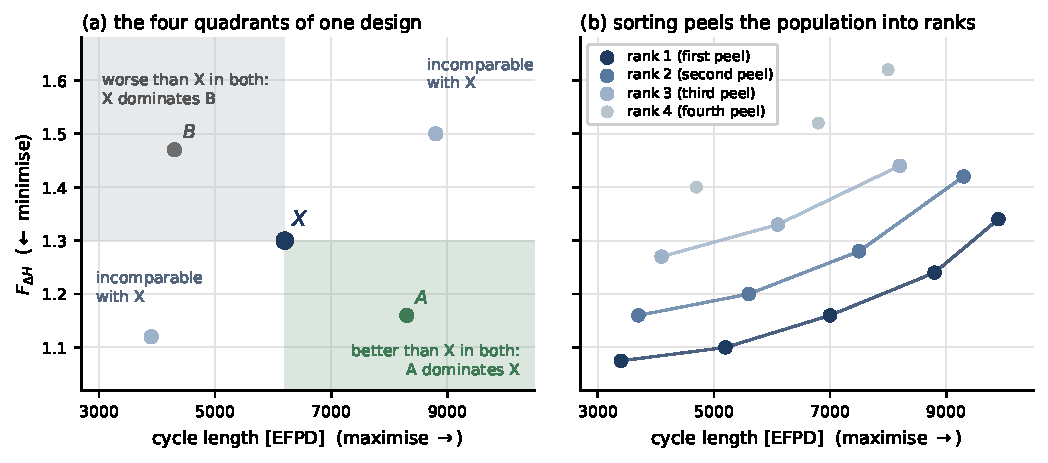
\includegraphics[width=\linewidth]{images/bg_nsga2_sorting.pdf}
  \caption{Dominance and non-dominated sorting.}
  \label{fig:bg-nsga2-sorting}
\end{figure}

\subsubsection*{Crowding distance}

The second ranking is a secondary selection criterion among designs of
the same rank, and it preserves the diversity of the population. It uses
the \emph{crowding distance}, a density estimate that measures how
isolated a design is from its neighbours along the front, and designs
are compared through the crowded-comparison
operator~\cite{deb_nsga2_2002}.

\begin{equation}
d_i = \sum_{m=1}^{M}
\frac{f_m^{(i+1)} - f_m^{(i-1)}}{f_m^{\max} - f_m^{\min}}
\label{eq:crowding}
\end{equation}

\noindent where the symbols have the following meaning:

\begin{itemize}
  \item $d_i$ is the crowding distance of design $i$, dimensionless,
        because each summand is normalised.

  \item $M$ is the number of objectives, equal to 2 in this thesis.

  \item $f_m^{(i+1)}$ and $f_m^{(i-1)}$ are the values of objective $m$
        for the two neighbours of design $i$ when its rank is sorted
        along that objective, in the units of objective $m$.

  \item $f_m^{\max}$ and $f_m^{\min}$ are the extreme values of
        objective $m$ within the rank, in the same units.

  \item The two boundary designs of each rank receive an infinite
        crowding distance, so the extremes of the front are never
        discarded.
\end{itemize}

Geometrically, $d_i$ is the normalised perimeter of the box spanned by
the two neighbours of design $i$, shown in
Figure~\ref{fig:bg-nsga2-crowding}.

A design in a sparsely populated stretch of the front has distant
neighbours, a large box and a large $d_i$. Keeping it preserves a
trade-off option that no other design represents. A design inside a
tight cluster is nearly redundant and is the first to be discarded.

Selection then follows one rule with one tie-breaker:

\begin{enumerate}
  \item The lower rank wins.

  \item At equal rank, the larger crowding distance wins.
\end{enumerate}

\begin{figure}[!tbp]
  \centering
  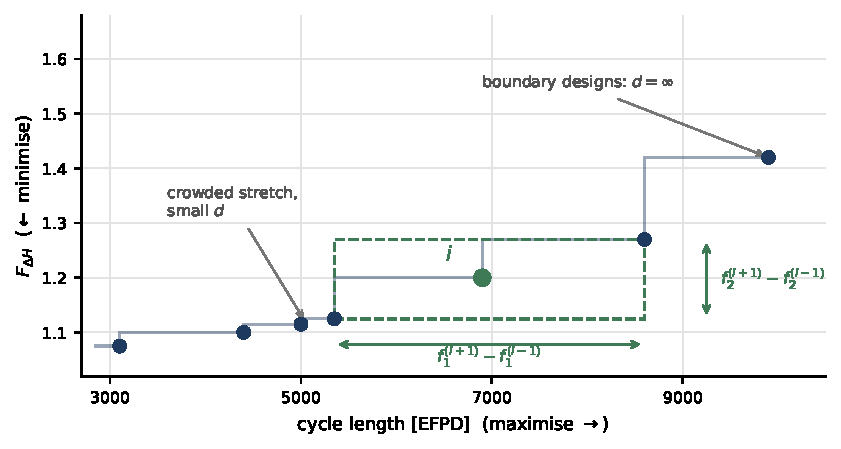
\includegraphics[width=0.8\linewidth]{images/bg_nsga2_crowding.pdf}
  \caption{Crowding distance of Equation~\eqref{eq:crowding}.}
  \label{fig:bg-nsga2-crowding}
\end{figure}

\subsubsection*{Constrained domination}

A constrained problem adds a difficulty. Most designs the search
generates violate at least one constraint, and simply discarding them
would leave selection with nothing to act on.

In the extreme case of a population with no feasible member at all,
discarding infeasible designs leaves no design to rank. The selection
operator then has no basis for preferring one design over another, and
the search loses all selection pressure. NSGA-II instead extends
dominance so that any two designs can always be compared, using the
total constraint violation~\cite{deb_nsga2_2002}.

\begin{equation}
V(\mathbf{x}) = \sum_{j=1}^{n_g} \max\bigl( 0,\, g_j(\mathbf{x}) \bigr)
\label{eq:violation}
\end{equation}

\noindent where the symbols have the following meaning:

\begin{itemize}
  \item $V(\mathbf{x})$ is the total constraint violation of design
        $\mathbf{x}$, dimensionless, equal to zero exactly when the
        design is feasible.

  \item $g_j(\mathbf{x})$ is the $j$-th constraint of
        Table~\ref{tab:constraints} in normalised form, dimensionless,
        feasible when non-positive.

  \item $n_g$ is the number of active inequality constraints of the
        campaign, dimensionless. It changes between campaigns, as stated
        with Equation~\eqref{eq:constraint_form}.

  \item $\max(0, \cdot)$ keeps only the violated part, so satisfied
        constraints contribute nothing and cannot compensate for
        violated ones.
\end{itemize}

\emph{Constrained domination} compares any pair of designs by three
rules, applied in order, restating Definition~1 of
Deb et al.~\cite{deb_nsga2_2002}:

\begin{enumerate}
  \item A feasible design always beats an infeasible one.

  \item Between two infeasible designs, the smaller total violation
        $V$ wins. Objective values are ignored.

  \item Between two feasible designs, Pareto dominance decides,
        %
        \begin{equation}
        \begin{split}
          \mathbf{x}^{(a)} \prec \mathbf{x}^{(b)}
          \iff
          & \forall i \in \{1,2\} :
            f_i\bigl(\mathbf{x}^{(a)}\bigr) \le f_i\bigl(\mathbf{x}^{(b)}\bigr) \\
          & \wedge\
            \exists j \in \{1,2\} :
            f_j\bigl(\mathbf{x}^{(a)}\bigr) < f_j\bigl(\mathbf{x}^{(b)}\bigr)
        \end{split}
        \label{eq:pareto-dominance-feasible}
        \end{equation}
        %
        The symbols carry the following meaning.
        \begin{itemize}
          \item $\mathbf{x}^{(a)}, \mathbf{x}^{(b)}$: two feasible
                design vectors, dimensionless.
          \item $\prec$: the dominance relation, read as
                \emph{dominates}, dimensionless.
          \item $f_1$: the cycle length in Effective Full Power Days
                (EFPD), negated so that maximisation becomes
                minimisation, in days.
          \item $f_2$: the radial enthalpy-rise hot-channel factor
                $F_{\Delta H}$, dimensionless.
          \item $i, j$: objective indices, dimensionless.
        \end{itemize}
        If neither design dominates the other, the two are mutually
        non-dominated. The crowded-comparison operator then prefers the
        design of lower non-domination rank and, at equal rank, the
        design with the larger crowding distance of
        Equation~\eqref{eq:crowding}~\cite{deb_nsga2_2002}.
\end{enumerate}

Figure~\ref{fig:bg-nsga2-thesis}(a) shows the three rules acting on a
mixed population. Rule 2 keeps a fully infeasible population
completely ordered, so selection still moves toward the feasible
region instead of stalling.

\begin{figure}[!tbp]
  \centering
  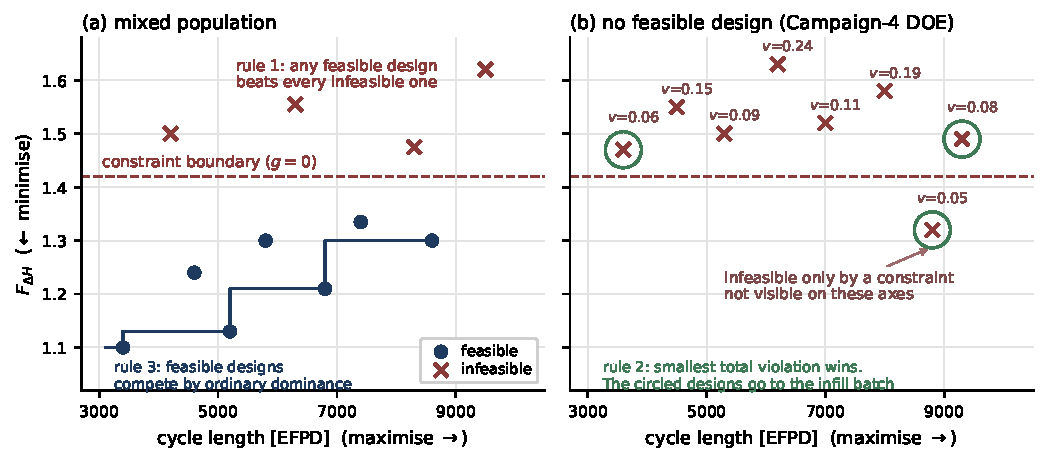
\includegraphics[width=\linewidth]{images/bg_nsga2_thesis.pdf}
  \caption{Constrained domination on illustrative data.}
  \label{fig:bg-nsga2-thesis}
\end{figure}

\subsubsection*{One generation}
With the comparisons in place, one elitist generation of NSGA-II
follows the main loop of Deb et al.~\cite{deb_nsga2_2002}.
Figure~\ref{fig:bg-nsga2-generation}, adapted from Figure~2 of that
paper, traces it:

\begin{enumerate}
  \item Create the offspring population $Q_t$ from the parent
        population $P_t$ of size $N$ by binary tournament selection
        under the comparisons above, followed by crossover and
        mutation.
  \item Pool parents and offspring into $R_t = P_t \cup Q_t$, $2N$
        designs in total. Every parent competes again, so the best
        designs found so far cannot be lost. This is the elitism of
        the algorithm.
  \item Sort $R_t$ into fronts $F_1, F_2, \ldots$ by non-dominated
        sorting under constrained domination.
  \item Fill the next population $P_{t+1}$ front by front until a
        front no longer fits entirely.
  \item Fill the remaining places from that first overfull front, $F_3$
        in the figure, in decreasing order of crowding distance. Reject
        the rest of that front and all lower fronts.
  \item Repeat until the generation budget is exhausted. The first
        front of the final population is the candidate Pareto set.
\end{enumerate}

\begin{figure}[!tbp]
  \centering
  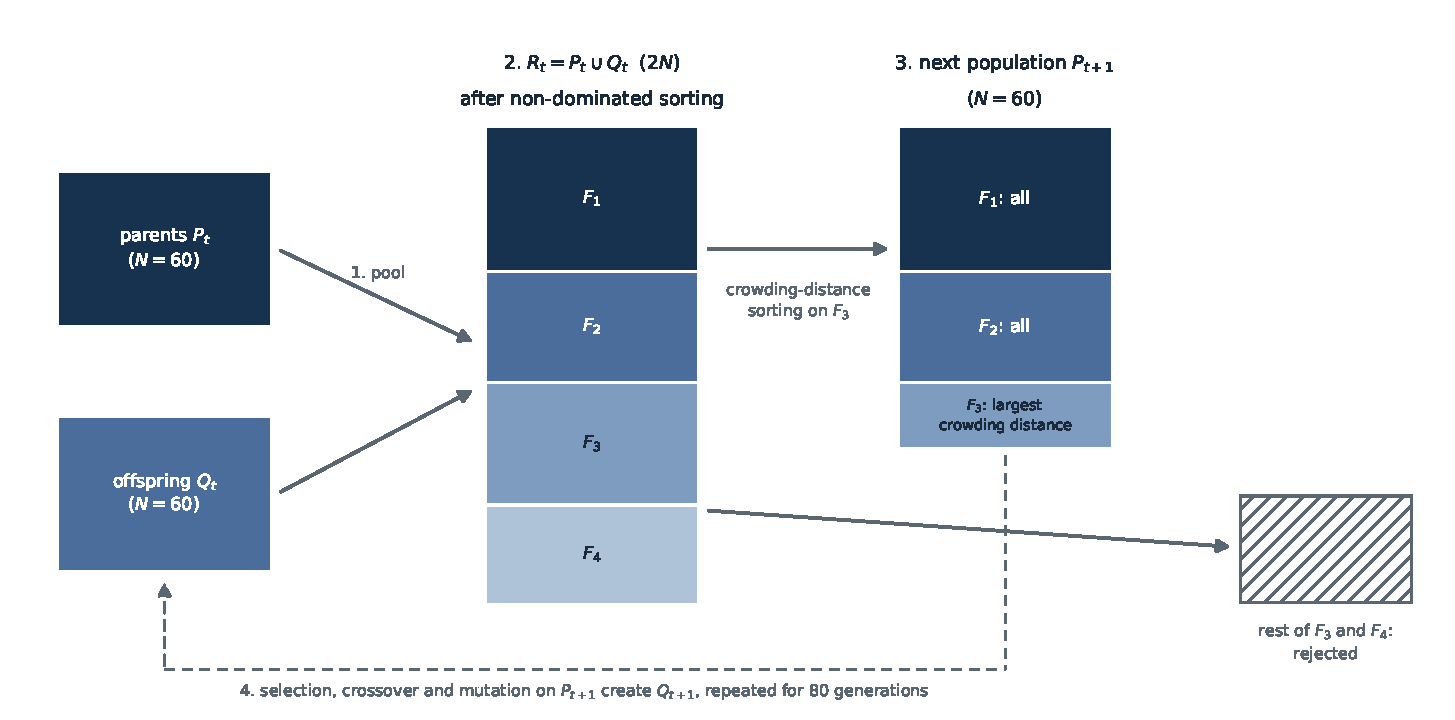
\includegraphics[width=0.95\linewidth]{images/bg_nsga2_generation.pdf}
  \caption[One elitist generation of NSGA-II]{One elitist generation of NSGA-II.\newline Figure adapted from~\cite{deb_nsga2_2002}.}
  \label{fig:bg-nsga2-generation}
\end{figure}

The population is defined by the settings of the campaign:

\begin{itemize}
  \item It lives in the design space of Table~\ref{tab:design-space},
        handled internally on the unit hypercube.

  \item It is judged on the two objectives of
        Section~\ref{sec:objective_functions}, with EFPD negated.

  \item It is subject to the constraints of Table~\ref{tab:constraints}
        in the $g \le 0$ convention that
        Equation~\eqref{eq:violation} consumes.
\end{itemize}

The number of design variables and the number of constraints both
change between campaigns. The values of each campaign are those of
Equation~\eqref{eq:constraint_form}.

NSGA-II never calls OpenMC. Each active-learning iteration searches
the Gaussian-process surrogate of Section~\ref{sec:bg-gp} with a
population of 300 evolved for 400 generations from Campaign 6, and of
60 for 80 generations before it (Section~\ref{sec:meth-nsga-setting}),
initialised by Latin hypercube sampling with a fresh random seed. One complete search
therefore costs seconds, instead of the thousands of transport
evaluations it replaces.

Constrained domination also kept the search alive at the Campaign-4
design of experiments, where all 36 designs were infeasible and
selection was governed entirely by rule 2. The final population is then
ranked by total violation, and its least-infeasible members are handed
to the infill step. This is the constraint-violation-driven mode of
Section~\ref{sec:res-c4}, drawn in Figure~\ref{fig:bg-nsga2-thesis}(b).

In that figure, the design with $V = 0.05$ lies below the dashed
boundary on $F_{\Delta H}$ and would look feasible if only its position
in the objective plane were inspected. It is infeasible nonetheless,
because it violates a constraint on a quantity that is not an
objective. Most constraints of Table~\ref{tab:constraints} act on such
quantities, among them the beginning-of-life multiplication factor and
the enrichment cap. The feasibility of a design, and its total violation
$V$, therefore cannot be inferred from its position in the objective
plane, and $V$ is computed from every constraint of the table.

\FloatBarrier


\subsection{Gaussian-process surrogates}
\label{sec:bg-gp}

A surrogate is a statistical stand-in for the expensive code, trained
on the designs evaluated so far and consulted everywhere
else~\cite{forrester_book_2008}. The search of the previous subsection
needs thousands of evaluations per iteration, and the surrogate is what
makes them affordable.

A Gaussian process (GP) is the surrogate family used here. Before any
design is evaluated, the GP treats the unknown objective as a random
function, and this prior distribution over functions expresses what is
assumed about the objective in advance. The prior is specified
completely by two functions~\cite{rasmussen_gp_2006}:

\begin{itemize}
  \item The mean function, the value expected at any design before data
        are available.

  \item The covariance kernel, which states how strongly the outputs of
        two designs are expected to vary together, as a function of
        their distance in the design space.
\end{itemize}

Conditioning the GP on the evaluated designs updates the prior with
Bayes' rule, so that the distribution becomes consistent with the
observed results. The updated distribution is the posterior. Its mean is
the prediction of the surrogate, and with the noise term used in this
work it passes close to, not exactly through, the evaluated values. Its
variance is the uncertainty of that prediction. It is small near
evaluated designs and grows with the distance from them, where the data
constrain the function least~\cite{rasmussen_gp_2006}.

Figure~\ref{fig:bg-gp} illustrates the posterior mean and variance,
together with the growth of the predictive uncertainty away from the
data that active learning exploits. The reasoning proceeds in four steps:

\begin{enumerate}
  \item Assume similarity: designs that are close in the design space
        should produce similar objective values.

  \item Encode that assumption in a kernel $k(\mathbf{x},\mathbf{x}')$,
        a function that returns the assumed covariance between the
        outputs of two designs from their distance.

  \item Condition on the archive of evaluated designs, that is, update
        the prior with the OpenMC results of every design evaluated so
        far, so that the predictions become consistent with them.

  \item Evaluate the posterior predictive distribution at any untried
        design, which gives its predicted mean and its predictive
        standard deviation.
\end{enumerate}

The kernel used in this work is the anisotropic Mat\'ern covariance
with smoothness $\nu = 5/2$, plus a white-noise
term~\cite{rasmussen_gp_2006}. Each of its three features answers a
property of the problem:

\begin{itemize}
  \item The Mat\'ern form with $\nu = 5/2$ gives functions that are twice
        differentiable. The squared-exponential kernel, the other common
        choice, gives infinitely differentiable functions, a smoothness
        that is considered unrealistic for most physical
        responses~\cite{rasmussen_gp_2006}.

  \item The anisotropy assigns one length scale to each design variable,
        because enrichment, gadolinia content, poisoned-pin count and
        reflector thickness change the objectives at different rates.

  \item The white-noise term represents the Monte Carlo noise of every
        evaluation, so the posterior mean is not forced through noisy
        values.
\end{itemize}

The choice follows common practice and was not compared against other
kernels in this work.

\begin{equation}
k(\mathbf{x}, \mathbf{x}')
= \sigma_f^{2}
\left( 1 + \sqrt{5}\,r + \tfrac{5}{3}\,r^{2} \right)
\exp\!\left( -\sqrt{5}\,r \right)
+ \sigma_n^{2}\,\delta_{\mathbf{x}\mathbf{x}'}
\label{eq:kernel}
\end{equation}

\begin{equation}
r = \left[ \sum_{d=1}^{D}
\frac{(x_d - x'_d)^{2}}{\ell_d^{\,2}} \right]^{1/2}
\label{eq:kernel-r}
\end{equation}

\noindent where the symbols have the following meaning:

\begin{itemize}
  \item $k(\mathbf{x}, \mathbf{x}')$ is the covariance between the
        outputs at designs $\mathbf{x}$ and $\mathbf{x}'$, in the
        squared units of the modelled output.

  \item $\sigma_f^{2}$ is the signal variance, in the squared units of
        the output, setting the overall scale of variation.

  \item $r$ is the scaled distance between the two designs,
        dimensionless.

  \item $x_d$ and $x'_d$ are the $d$-th components of the two design
        vectors after standardisation, dimensionless.

  \item $D$ is the number of design variables, equal to 5 in Campaigns
        1 to 4.

  \item $\ell_d$ is the length-scale of variable $d$, dimensionless
        after standardisation. One length-scale per variable is the
        automatic relevance determination (ARD) structure.

  \item $\sigma_n^{2}$ is the noise variance, in the squared units of
        the output, absorbing the evaluation noise.

  \item $\delta_{\mathbf{x}\mathbf{x}'}$ is the Kronecker delta, equal
        to 1 when the two designs coincide and 0 otherwise,
        dimensionless.
\end{itemize}

Conditioning the prior on $n$ archive evaluations gives the posterior
prediction at any new design $\mathbf{x}$~\cite{rasmussen_gp_2006}.

\begin{equation}
\mu_*(\mathbf{x})
= \mathbf{k}_*^{\mathsf T}
\left( \mathbf{K} + \sigma_n^{2}\,\mathbf{I} \right)^{-1} \mathbf{y}
\label{eq:gp-mean}
\end{equation}

\begin{equation}
\sigma_*^{2}(\mathbf{x})
= k(\mathbf{x}, \mathbf{x})
- \mathbf{k}_*^{\mathsf T}
\left( \mathbf{K} + \sigma_n^{2}\,\mathbf{I} \right)^{-1} \mathbf{k}_*
\label{eq:gp-var}
\end{equation}

\noindent where the symbols have the following meaning:

\begin{itemize}
  \item $\mu_*(\mathbf{x})$ is the predicted mean at design
        $\mathbf{x}$, in the units of the output.

  \item $\sigma_*^{2}(\mathbf{x})$ is the predictive variance of the
        underlying response at $\mathbf{x}$, in the squared units of
        the output.

  \item $\mathbf{y}$ is the vector of the $n$ archive outputs, in the
        units of the output.

  \item $\mathbf{K}$ is the $n \times n$ matrix of kernel values
        between archive designs, with entries
        $K_{ij} = k(\mathbf{x}_i, \mathbf{x}_j)$.

  \item $\mathbf{k}_*$ is the vector of kernel values between the new
        design and each archive design, with entries
        $k(\mathbf{x}_i, \mathbf{x})$.

  \item $\mathbf{I}$ is the $n \times n$ identity matrix,
        dimensionless.

  \item $n$ is the number of archive evaluations, dimensionless.
\end{itemize}

The two equations have a simple reading~\cite{rasmussen_gp_2006}:

\begin{itemize}
  \item Equation~\eqref{eq:gp-mean} says the prediction is a weighted
        average of the archive outputs, with weights set by similarity.

  \item Equation~\eqref{eq:gp-var} says the uncertainty shrinks near
        evaluated designs and grows away from them, which is exactly the
        information the active-learning loop consumes.
\end{itemize}

Two kernel features carry particular weight in this work:

\begin{enumerate}
  \item The ARD structure learns one length-scale per design variable.
        A variable along which the response is flat is assigned a large
        length-scale, so the fitted length-scales rank the variables by
        their influence on each output.

  \item The white-noise component absorbs the evaluation noise. Two
        properties of this component matter:
        \begin{enumerate}
          \item its assumption of independent and identically
                distributed noise across designs is violated by a
                shared random seed, which motivates the per-design
                seeding policy adopted in Campaign~3,
          \item its fitted magnitude is an upper bound on the true
                Monte Carlo noise, so the excess over the measured
                noise quantifies residual model misfit.
        \end{enumerate}
\end{enumerate}

\begin{figure}[htbp]
  \centering
  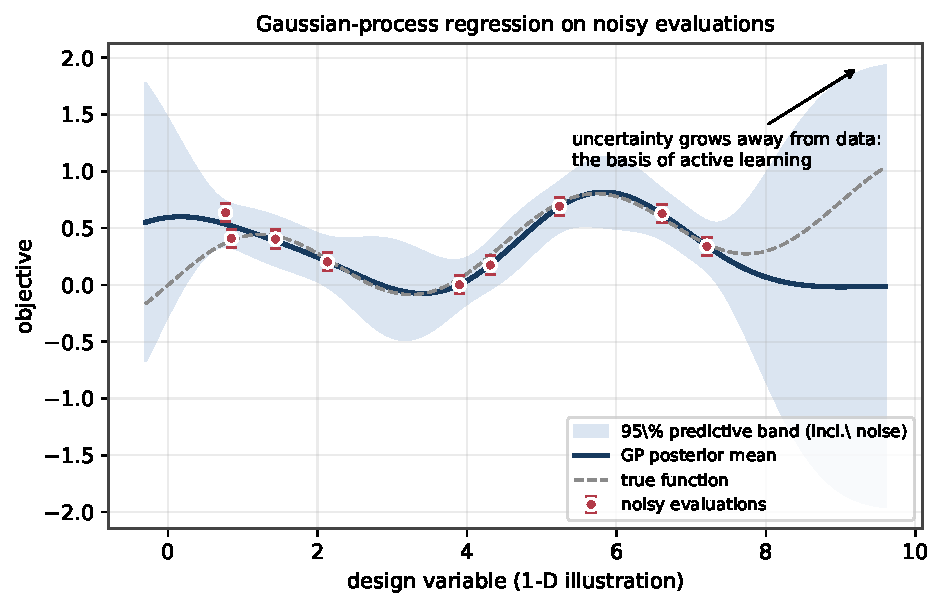
\includegraphics[width=0.8\linewidth]{images/bg_gp.pdf}
  \caption{Gaussian-process regression on noisy evaluations: posterior mean and 95\% predictive band.}
  \label{fig:bg-gp}
\end{figure}

The settings with which this surrogate is used in the campaigns are
fixed in Section~\ref{sec:meth-loop-settings}. They cover the
standardisation of inputs and outputs, one Gaussian process per output,
and the refitting of the hyperparameters at every iteration.

\subsection{The active-learning loop}
\label{sec:bg-al}

The surrogate is only as good as its training set, and the training set
is expensive. Active learning is the strategy of spending the
evaluation budget where it teaches the model
most~\cite{forrester_book_2008}.

The starting set must cover the design space before anything is known
about it. The initial design of experiments uses Latin hypercube
sampling (LHS)~\cite{mckay_lhs_1979}, built in three steps:

\begin{enumerate}
  \item The range of every variable is divided into as many equal
        slices as there are samples.

  \item Exactly one sample is placed in each slice of each variable.

  \item The combinations are randomly permuted.
\end{enumerate}

The guarantee is one-dimensional coverage: no variable is left with an
unexplored stretch. Uniform random sampling cannot promise that at
equal budget.

From there the campaign follows the dual-stage loop of
Figure~\ref{fig:bg-al}, whose steps repeat until the stopping rule is
met:

\begin{enumerate}
  \item Draw the LHS design of experiments and evaluate it with OpenMC,
        the expensive truth of Section~\ref{sec:meth-fidelity}.

  \item Fit the Gaussian-process surrogates of
        Section~\ref{sec:bg-gp}, objectives and constraints, on the
        whole cumulative archive and not on the newest batch alone.

  \item Run the NSGA-II search of Section~\ref{sec:bg-nsga2} on the
        surrogate. Its final rank-1 population is the candidate set.
        If the surrogate predicts no feasible region, the
        least-infeasible members take that role.

  \item Select the infill batch, the designs that are evaluated with
        OpenMC in this iteration, from the candidates. The selection
        proceeds in five sub-steps, detailed in
        Section~\ref{sec:meth-acq}:
        %
        \begin{enumerate}[label=\arabic{enumi}.\arabic*]
          \item Predict, for every candidate, the posterior standard
                deviation of each of the two objectives with
                Equation~\eqref{eq:gp-var}.

          \item Divide each standard deviation by the largest value of
                the same objective over the candidate set. The two
                objectives have different units, and the division gives
                them equal weight.

          \item Add the two normalised values. The sum is the
                uncertainty score of the candidate, and a high score
                marks a design whose predicted objectives rest on few
                nearby evaluations.

          \item Screen the candidates on the constraint surrogates.
                Candidates whose predicted constraints stay satisfied
                after a margin of $\kappa$ standard deviations rank first,
                by descending score. The others follow, from the least to
                the most likely to violate a constraint.

          \item Walk down the ranking and accept a candidate only if it
                lies at least a minimum normalised distance from every
                design of the archive and from the designs already
                accepted, which also excludes designs already evaluated.
                The walk stops when the batch is full. If the ranking runs
                out first, the minimum distance is halved and the walk is
                repeated.
        \end{enumerate}

        The candidate set and the uncertainty ranking play complementary
        roles:

        \begin{itemize}
          \item The candidate set supplies the \emph{exploitation}.
                Every candidate belongs to the rank-1 set of the surrogate
                search, so each is predicted to be among the best designs
                available.

          \item The uncertainty ranking supplies the
                \emph{exploration}. Among these promising designs, it
                sends to OpenMC those whose predictions are least
                supported by the data, so each evaluation tests a
                promising region and reduces the uncertainty where it is
                largest.
        \end{itemize}

  \item Evaluate the infill batch with OpenMC and append it to the
        archive.

  \item Record the state of the loop at the end of the iteration:
        %
        \begin{enumerate}[label=\arabic{enumi}.\arabic*]
          \item Recompute the hypervolume of Section~\ref{sec:bg-hv} on
                the updated archive.

          \item Write a checkpoint, a file holding the full archive of
                evaluated designs and their results.

          \item If the run is interrupted, for example by a machine
                failure, a loss of power or a software error, restart it
                from the last checkpoint.
        \end{enumerate}

        Only the OpenMC evaluations of the iteration in progress are
        lost, at most one infill batch, and no completed evaluation has
        to be repeated. The checkpoint was introduced after a crash
        during Campaign~4 discarded six completed evaluations.

  \item Between blocks of iterations, apply the stopping rule of
        Section~\ref{sec:meth-loop}. At convergence, pass the finalists
        to the high-fidelity confirmation of
        Section~\ref{sec:meth-stats}.
\end{enumerate}

The separation between a cheap search stage and an expensive
confirmation stage is the two-tier principle that recurs throughout the
thesis.

\begin{figure}[htbp]
  \centering
  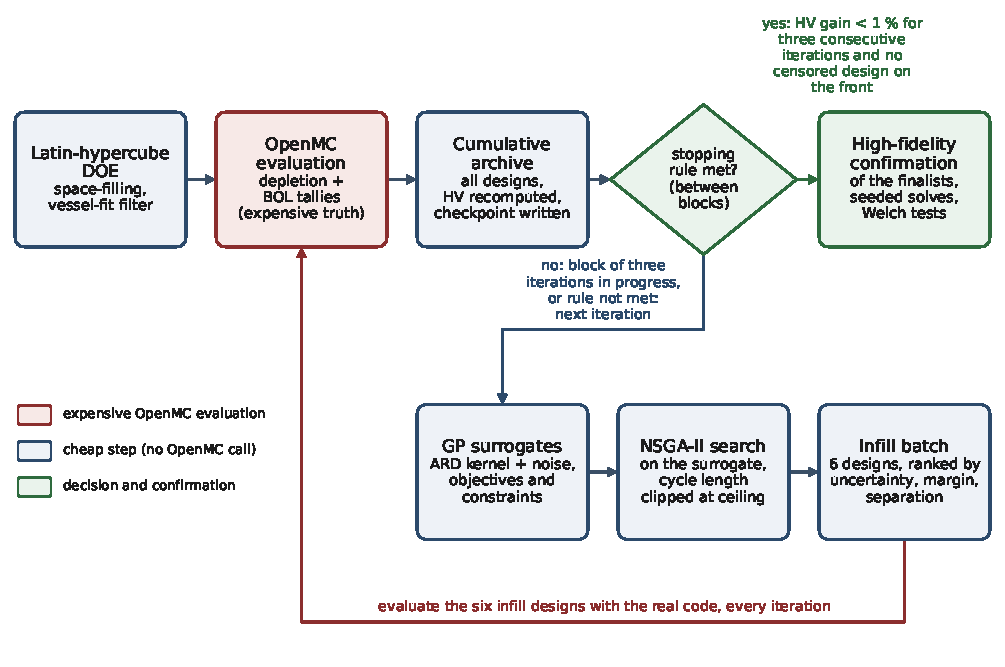
\includegraphics[width=0.95\linewidth]{images/bg_al_loop.pdf}
  \caption{The dual-stage surrogate-assisted active-learning loop as implemented.}
  \label{fig:bg-al}
\end{figure}

The design of experiments, the infill batch, the block structure and the
budget with which the loop was run are fixed in
Section~\ref{sec:meth-loop-settings}. They are stated once there, next
to the acquisition function they feed.


% =====================================================================
%  methodology.tex  --  Chapter 4 (single file; the design-basis text of
%  methodology_design_basis_01JUL.tex is MERGED in Section 4.1 -- no
%  \input needed, retire that file from Overleaf).
%
%  REVISION NOTE (this version):
%   1. Formal definitions of quantities shared across chapters now live
%      in the background chapter: F_dH is eq:fdh_definition and the
%      burnup-to-EFPD conversion is eq:efpd. This chapter defines only
%      its own constructs: the optimisation problem, the constraints,
%      the end-of-cycle criterion (eq:eoc, eq:eoc-k), the Monte Carlo
%      estimator (eq:fdh_estimator) and the k-target (eq:ktarget).
%   2. The duplicated \label{sec:meth-core-objective} is removed; the
%      label belongs only to the proxy-validation section.
%   3. The undefined references sec:peaking_statistics,
%      sec:selection_methodology and sec:stopping_rules are replaced by
%      sec:meth-stats and sec:meth-loop.
%   4. Every displayed formula is followed by a term-by-term list with
%      units. Enumerations set as lists. No semicolons, no em dashes.
%
%  Requires: booktabs, amsmath, graphicx.
%  Figures: figs_thesis/th_model_geometry.pdf (generator committed).
% =====================================================================
\providecommand{\openpoint}[1]{\par\noindent\fbox{\parbox{0.97\linewidth}{%
  \textbf{Open point:} #1}}\par}

\chapter{Methodology}
\label{ch:methodology}

This chapter is ordered along the calculation chain, and each part
answers one question:

\begin{enumerate}
  \item \textbf{What is modelled?} The design basis, the reactor model
        and the soluble boron of the coolant.

  \item \textbf{What is asked of the model?} The optimisation problem,
        its objectives and constraints, the structure of the campaigns
        and the design space and formulation of Campaigns 8 and 9.

  \item \textbf{Which derived quantities does the problem need?} The
        leakage-corrected reactivity target, the radial enrichment
        zoning, the burnup limits and the MTC boron limit set by
        the moderator temperature coefficient.

  \item \textbf{How is a design evaluated and the next batch
        chosen?} The transport fidelity and seeding, and the
        surrogate-assisted loop that drives the search.

  \item \textbf{How is the method checked?} The validation of the
        peaking proxy and the validation of the optimisation framework.

  \item \textbf{When may the active batches of a solve be scored?}
        The source-convergence diagnostic, which decides whether the
        fission source of a transport solve was stationary before its
        active batches began.

  \item \textbf{How is a result reproduced?} The computing
        environments, the seed policy and the archived checkpoints.
\end{enumerate}

The definitions shared with the other chapters are not repeated here.
The radial peaking factor and the burnup-to-cycle-length conversion are
defined in Chapter~\ref{ch:background}, and the results of every
campaign are reported in Chapter~\ref{ch:results}.

\section{Design basis and technological conservatism}
\label{sec:design-basis}

The reference small modular reactor is conceived under a deliberate
constraint of \emph{technological conservatism}, which sets two criteria
for the design basis.

\begin{enumerate}
  \item \textbf{Domestic industrial base:} the fuel technology of the
        core is restricted to what is already qualified and in series
        production in Brazil.

  \item \textbf{Western standard PWR practice:} every choice the
        domestic base leaves open is taken from the most widely
        fabricated and best-benchmarked technology in service, which
        for the lattice is the $17\times17$ Westinghouse-type assembly
        of the NuScale-like reference
        specification~\cite{nuscale_htp2_2017,nuscale_like_core_2024}.
        That specification is the published open description of a small
        modular PWR with a $17\times17$ lattice,
        and this work takes from it the geometry, the material
        compositions and the operating conditions that an OpenMC model
        requires. It is a source of inputs in this chapter, and the
        quantitative comparison against it is made in
        Chapter~\ref{ch:results}.
\end{enumerate}

To meet the mission objective, namely a long refuelling interval under
low-enriched uranium (LEU), the first criterion is relaxed on one
point. The enrichment is bounded by the LEU enrichment limit of \SI{19.75}{wt\%} of
Equation~\eqref{eq:leu-box} rather than by the 2 to \SI{5}{wt\%} of
current INB production~\cite{inb_resende}. Every other element of the
design is held inside the two criteria, and three of them follow
directly from those criteria:

\begin{enumerate}
  \item The fuel form is the one in national production: UO$_2$
        ceramic pellets in Zircaloy-4 cladding, fabricated by INB at
        Resende for Angra~1, a Westinghouse plant, and Angra~2, a
        Siemens
        plant~\cite{inb_montagem_ec,eletronuclear_angra1,eletronuclear_angra2}.

  \item The lattice is the $17\times17$ Westinghouse-type assembly,
        under the second criterion. The Angra units are $16\times16$,
        the geometry of an earlier plant generation, while the
        $17\times17$ is the most widely fabricated commercial geometry
        in service today. Its adoption is therefore an incremental
        industrialisation step for the same qualified fuel fabrication
        process, and it carries a validated basis for benchmarking this
        model against the open
        literature~\cite{nuscale_htp2_2017,nuscale_like_core_2024}.

  \item The excess reactivity is held down by gadolinia burnable
        absorbers, the burnable poison of the Angra~2
        fuel~\cite{angra2_gd_2018}. The gadolinia weight fraction and
        the number of poisoned pins are design variables of the
        search.
\end{enumerate}

The result of the work is therefore a set of core designs that this
industrial base can build and that the control system can hold.

\section{Reactor model}
\label{sec:reactor-model}

Two terms recur throughout this chapter. The evaluator is the code
that builds the OpenMC models of one candidate design, runs its
transport and depletion calculations and returns its objectives and
constraints. The archive is the database in which every evaluated
design is stored with its inputs and its results, and it is the record
from which Chapter~\ref{ch:results} is computed.

The model is built in OpenMC~0.15.3~\cite{romano_openmc_2015} with
ENDF/B-VII.1 data, from one parametric design dictionary driving three
fidelities: pin cell, $17\times17$ assembly, and the 32-assembly core.
Figure~\ref{fig:model-geometry} defines the geometry. Panel~(a) marks
the two enrichment zones, the 24 guide tubes and the central instrument
tube. The poisoned-pin patterns are not depicted there, since they are
given in Figure~\ref{fig:gd-ladder}. The ranges of the six design
variables of
Campaigns 5 to 7 are tabulated beneath the panels, where $p$ and
$t_\mathrm{refl}$ appear coupled by $g_\mathrm{geom}$. The numerical
basis is concentrated in Tables~\ref{tab:model-geometry}
and~\ref{tab:model-operating}.

\begin{figure}[htbp]
  \centering
  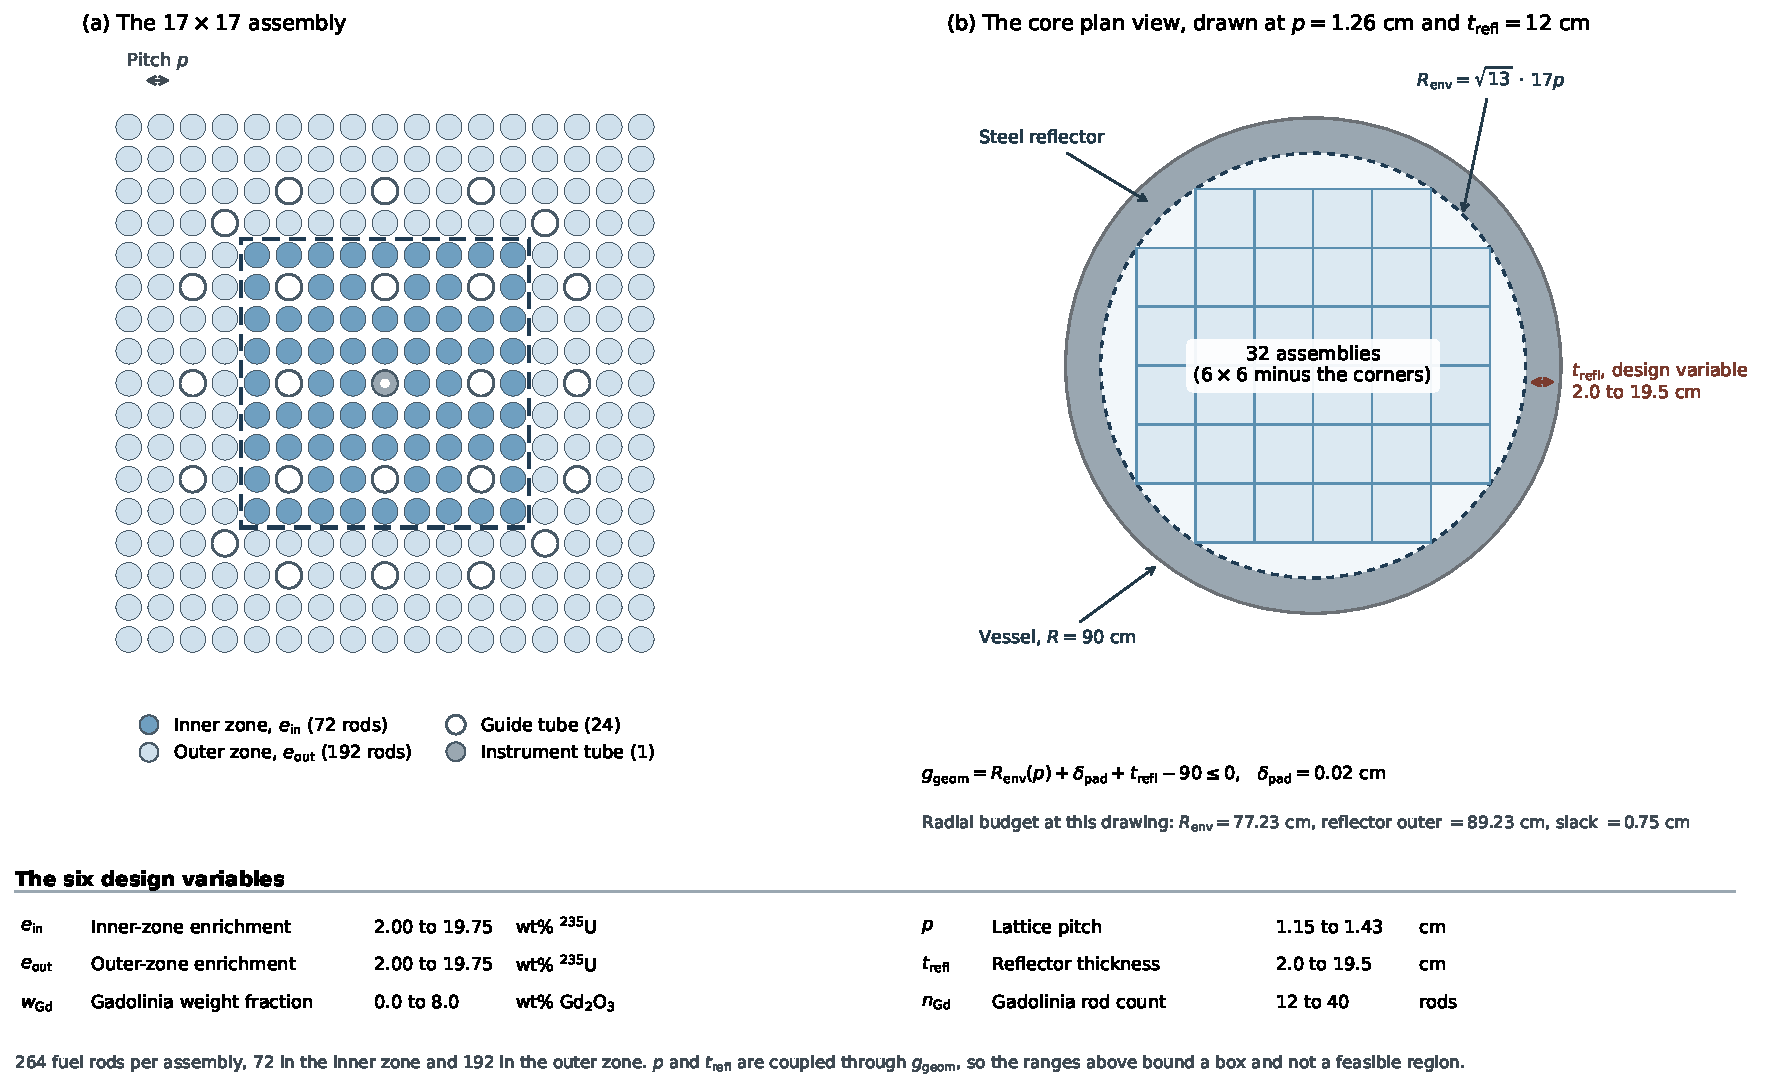
\includegraphics[width=\linewidth]{images/th_model_geometry.pdf}
  \caption[The reference model and the six-variable design space]{The reference model. (a)~The $17\times17$ assembly. (b)~The core plan view.}
  \label{fig:model-geometry}
\end{figure}

\begin{table}[htbp]
  \centering
  \caption{Geometry of the reference model.}
  \label{tab:model-geometry}
  \begin{tabular}{llc}
    \toprule
    Item & Value & Unit \\
    \midrule
    Fuel pellet outer radius & 0.406 & cm \\
    Cladding inner / outer radius & 0.414 / 0.475 & cm \\
    Guide-tube inner / outer radius & 0.572 / 0.612 & cm \\
    Lattice & $17\times17$: 264 rods, 24 GT, 1 IT & -- \\
    Inner enrichment zone & centred $9\times9$: 72 fuel rods (27\%) & -- \\
    Outer enrichment zone & 192 fuel rods (73\%) & -- \\
    Gd$_2$O$_3$ rods & 12 (C1--C4), discrete 12--40 (C5 on) & -- \\
    Active fuel height & 120 (heavy-metal mass only) & cm \\
    Core map & $6\times6$ minus corners = 32 assemblies & -- \\
    Reflector & stainless steel annulus, thickness $t_\mathrm{refl}$ & -- \\
    Vessel internal radius & 90 & cm \\
    \bottomrule
  \end{tabular}
\end{table}

The vessel internal radius is the 900\,mm inner radius of the simplified
vessel model dimensioned according to CTMSP~\cite{maruyama_2013}, as
detailed in Figure~\ref{fig:vessel-dimensioned}. The pin
and guide-tube dimensions follow NuScale-class
practice~\cite{nuscale_htp2_2017}. The core thermal power is the
48\,MW of thermal power that the Navy gives for the LABGENE
reactor~\cite{demartini_nuclep_2022}, within the 48 to 50\,MWth of the
academic literature~\cite{dinizcosta_2017}. The active height, the
enrichment zoning, the poisoned-pin pattern, the core map, the
reflector, the temperatures, the soluble boron concentration and the
nuclear data are modelling choices of this thesis.

\begin{table}[htbp]
  \centering
  \caption{Operating and material basis of the reference model.}
  \label{tab:model-operating}
  \begin{tabular}{llc}
    \toprule
    Item & Value & Unit \\
    \midrule
    Core thermal power & 48 & MW \\
    Specific power $P_\mathrm{spec}$ & 9.9834 & W/gHM \\
    Fuel / clad / moderator temperature & 900 / 600 / 580 & K \\
    Soluble boron (fixed, Sec.~\ref{sec:meth-boron}) & 1000 & ppm \\
    Nuclear data & ENDF/B-VII.1 + PWR chain & -- \\
    \bottomrule
  \end{tabular}
\end{table}

In three quantities the campaign model states its own value instead of
the one given by the reference specification. Each value is held fixed across the campaigns, so
that every design is evaluated on the same basis and the comparison
between designs is unaffected, and the effect of each on the absolute
result is measured in the three-dimensional confirmation.

\begin{enumerate}
  \item The heavy reflector is homogenised at \SI{90}{\%} steel by
        volume, a deliberately moderator-rich engineering estimate,
        against \SI{95.6}{\%} in the reference specification.

  \item The control rod absorber radius is \SI{0.433}{cm} for both
        absorbers, against \SI{0.423}{cm} for boron carbide and
        \SI{0.427}{cm} for silver-indium-cadmium in the reference specification.
        The clad radii, \num{0.4369} and \SI{0.484}{cm}, and the
        absorber number densities are those of the reference specification.

  \item The coolant density is \SI{0.72}{g/cm^3} at \SI{580}{K},
        against \SI{0.752}{g/cm^3} implied by the reference-specification number
        densities at its stated \SI{600}{K}. The boron mass fraction
        of \SI{1000}{ppm} is the same in both.
\end{enumerate}


\begin{figure}[htbp]
  \centering
  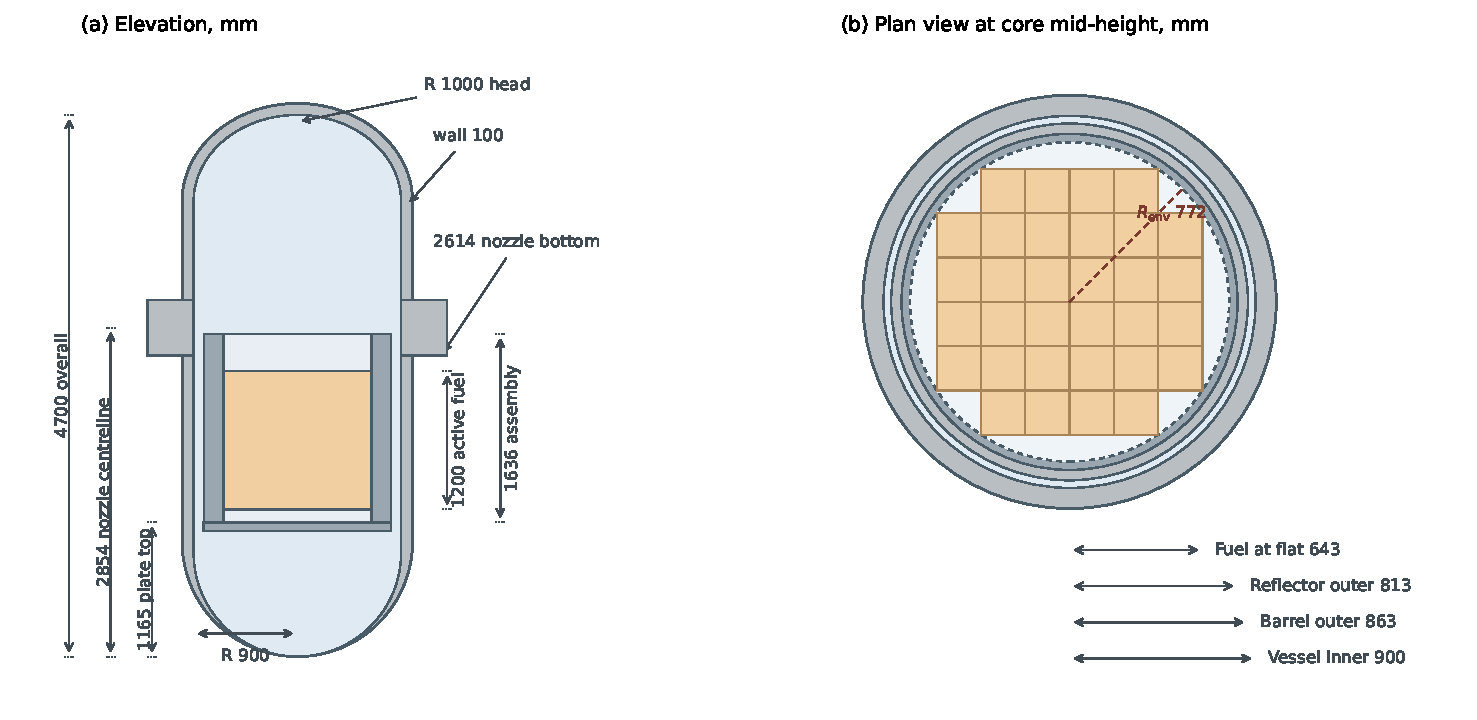
\includegraphics[width=\textwidth]{images/th_vessel_dimensioned}
  \caption{Elevation and plan view of the adopted vessel and core layout, in millimetres.}
  \label{fig:vessel-dimensioned}
\end{figure}

The dimensions of Figure~\ref{fig:vessel-dimensioned} have three
provenances, in the sense of the code table of
Table~\ref{tab:in-key}. The vessel envelope, with an overall height of 4700\,mm, a
cylindrical inner radius of 900\,mm, a wall thickness of 100\,mm and a
closure-head inner radius of 1000\,mm, is that of the simplified vessel
model dimensioned according to CTMSP~\cite{maruyama_2013}. The internal
elevations, the lower core plate and the coolant nozzle penetration,
were measured on that same drawing, which carries no dimension for
them, with the overall height as the scale reference, so they carry the
unquantified error of a graphical measurement. The structural components of the fuel assembly,
the nozzles, the end caps, the plenum spring and the spacer grids, keep
the sizes of the NuScale-like reference
specification~\cite{ez_aldeen_2025} without change.

The axial layout combines those two sources. The fixed components are
stacked above the lower core plate at their standard sizes, which
accounts for \SI{435.6}{mm} of the assembly, and the active fuel length
is the remainder up to the coolant nozzle penetration. That remainder is
\SI{1200}{mm}, against the \SI{2000}{mm} of the reference specification,
so the active length is set by the LABGENE-class envelope and not
inherited. The layout is therefore a standard fuel assembly, at
unchanged component sizes, fitted to the space this vessel leaves.

The active height of 120\,cm and the stainless steel reflector annulus
are modelling choices of this thesis, since no open source specifies the
reflector or the core barrel of LABGENE. The plan view of
Figure~\ref{fig:vessel-dimensioned} is constructed for a pin pitch of 1.26\,cm
and a minimum reflector thickness of 4.0\,cm.

\begin{figure}[htbp]
  \centering
  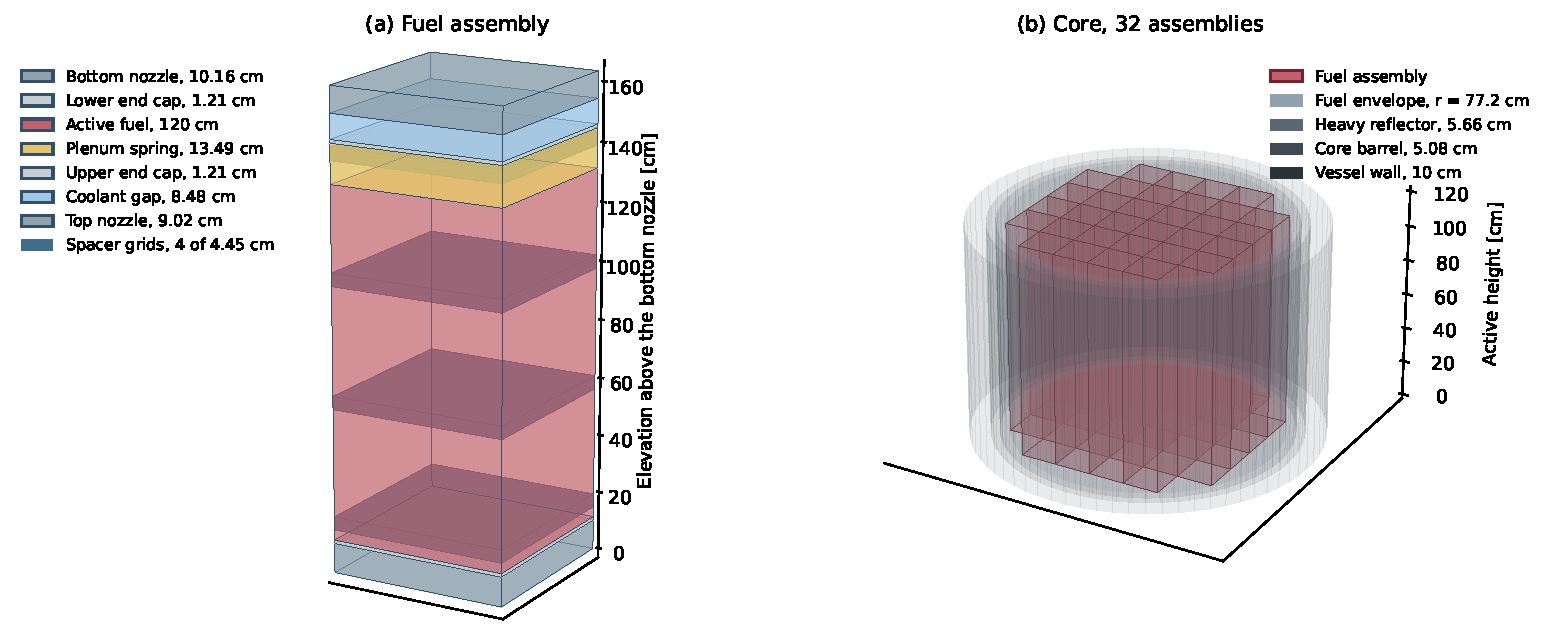
\includegraphics[width=\linewidth]{images/th_model_3d.pdf}
  \caption{The fuel assembly and the core in three dimensions.}
  \label{fig:model-3d}
\end{figure}

Figure~\ref{fig:model-3d} shows that assembly and the core in three
dimensions, and Table~\ref{tab:axial-layout} gives the axial layout
adopted for the three-dimensional core model. Elevations are measured
from the outer bottom of the lower head, with the assembly resting on
the lower core plate.

\begin{table}[htbp]
  \centering
  \caption{Axial layout of the fuel assembly in the three-dimensional core model, in millimetres.}
  \label{tab:axial-layout}
  \begin{tabular}{@{}lrrr@{}}
    \toprule
    \textbf{Item} & \textbf{Height} & \textbf{From} & \textbf{To} \\
    \midrule
    Bottom nozzle             &  101.6  & 1165.0 & 1266.6 \\
    Lower end cap             &   12.05 & 1266.6 & 1278.6 \\
    Active fuel               & 1200.0  & 1278.6 & 2478.6 \\
    Plenum spring             &  134.9  & 2478.6 & 2613.5 \\
    Upper end cap             &   12.05 & 2613.5 & 2625.6 \\
    Upper coolant gap         &   84.8  & 2625.6 & 2710.4 \\
    Top nozzle                &   90.2  & 2710.4 & 2800.6 \\
    \addlinespace
    Spacer grids, 4 of        &   44.45 & 1314.2 & 2600.8 \\
    \bottomrule
  \end{tabular}
\end{table}

The spacer grids take their materials and their height from the
reference specification, one of Inconel followed by three of Zircaloy.
Their number and their spacing do not follow it. The specification
carries five grids at a span of \SI{510.5}{mm} over \SI{2000}{mm} of
active fuel, whereas the shorter active length adopted here carries
four at an equal span of \SI{414}{mm}, of which three are inside the
active fuel and the fourth inside the plenum. The assembly is
\SI{1635.6}{mm} long.

\subsection{Treatment of the barrel and the downcomer in the campaign model}
\label{sec:meth-barrel}

The campaign transport model terminates in a vacuum boundary at the
outer surface of the heavy reflector, so the core barrel, the downcomer
water and the vessel wall of Figure~\ref{fig:vessel-dimensioned} carry
no transport solution. The radial space they occupy is still reserved
in the geometry, from Campaign 8 onward, by the vessel-fit constraint
of Equation~\eqref{eq:ggeom}, which holds the envelope of the core and
its reflector inside the \SI{90}{cm} vessel inner radius. No design is
therefore accepted that would leave those structures insufficient
radial clearance.

What the omission removes is the albedo of the region behind the
reflector, the fraction of the neutrons leaking from the reflector that
scatter back into the core. That albedo is set by materials and
thicknesses that are the same in every design, and it responds only
weakly to the design variables, so it raises every eigenvalue by nearly
the same amount, shifts every cycle length together and leaves the
ordering of the front unchanged. For the controllability constraint of
Section~\ref{sec:meth-ctrl} the omission acts in the non-conservative
direction. A vacuum boundary imposes zero albedo, so the modelled core
is less reactive than the real one in both rod states and the modelled
rodded core is more subcritical than the real one. That constraint acts on
the rodded eigenvalue itself rather than on a bank worth, so the albedo
does not cancel between the two states, and a design whose rodded
eigenvalue is close to the limit may pass the constraint while the real
geometry does not. The albedo is expected to be small, since the heavy
reflector already returns most of the neutrons that leave the core, and
the downcomer sensitivity of Section~\ref{sec:res-c8-3d}, in which the
downcomer is thinned from \SI{2.0}{cm} to \SI{3.7}{cm}, moves the
unrodded three-dimensional eigenvalue of design C8-47 by
\SI{-33}{pcm}. That bounds the sensitivity to the downcomer thickness
and not the albedo against a vacuum boundary, which was not quantified
in this work. The
three-dimensional confirmation model of Section~\ref{sec:res-c8-3d}
carries the barrel, the downcomer and the vessel wall explicitly, and
it introduces the axial leakage at the same time, so it does not
separate the two effects.

\section{Soluble boron treatment}
\label{sec:meth-boron}

The coolant carries a constant concentration of \SI{1000}{ppm} of
natural boron in every campaign of this work. The value is taken from
the operating conditions of the NuScale-like neutronics reference specification
defined by Fridman, Bilodid and
Valtavirta~\cite{fridman_nuscale_benchmark_2023}, together with the
uniform fuel temperature of \SI{900}{\kelvin} adopted in
Table~\ref{tab:model-operating}. The cladding and the steel structures
of that table are at \SI{600}{\kelvin}, and the coolant, which is also
the moderator, at \SI{580}{\kelvin}.

The concentration is a fixed modelling parameter, and no campaign of
this work exposes it to the optimiser as a design variable. Campaign 9 does carry a boron
quantity in its formulation, the critical concentration at the
operating maximum. That quantity is an objective, computed from each
evaluated design and minimised (Section~\ref{sec:meth-c9}), while the
depletion of that campaign still runs at the fixed \SI{1000}{ppm}.

The specification is static, at Beginning of Life (BOL), and does not
specify a depletion history. The extension of those
conditions to a depleted core is an assumption of the present work and
is treated as such in Section~\ref{sec:meth-boron-limits}.

\subsection{Basis for the choice}
\label{sec:meth-boron-basis}

Soluble boron is one of the reactivity-control methods of the boron-controlled
PWR lineage from which the present core
inherits its assembly geometry, and it is retained by the majority of
land-based light-water Small Modular Reactor (SMR) concepts now under
development. Four considerations support retaining it here.

\begin{enumerate}
  \item \textbf{Traceability of the reference conditions:} the
        NuScale-like reference specification provides a published
        input set, a
        Monte Carlo reference solution obtained with
        Serpent~\cite{fridman_nuscale_benchmark_2023}, and an
        independent reproduction with the same transport code and
        nuclear data library used in this work, namely OpenMC with
        ENDF/B-VII.1~\cite{ez_aldeen_2025}. That
        reproduction reports agreement within 16 to \SI{31}{pcm} in the
        effective multiplication factor and a root mean square relative
        difference below \SI{0.11}{\percent} in assembly radial power.
        No soluble boron specification for the LABGENE-class core that
        motivates the study is available in the open literature.
  \item \textbf{Containment of the design space:} soluble boron and the
        two absorber-related design variables, the gadolinium oxide
        (\ce{Gd2O3}) weight fraction and the gadolinium-bearing pin
        count, act on the same physical quantity, namely the excess
        reactivity available at beginning of life. Allowing boron to
        vary would make the study partly a study of boron rather than
        of the fuel and lattice variables under investigation.
  \item \textbf{Scope of the safety demonstration:} a
        Soluble-Boron-Free (SBF) core transfers the entire
        excess-reactivity budget to the burnable absorbers and the
        control rods, so its reactivity control rests on the control
        rod bank configuration. Three statements bound what this work
        establishes about that configuration.

        \begin{enumerate}[label=\theenumi.\arabic*, ref=\theenumi.\arabic*]
          \item \textbf{The configuration of the prototype is not
                available:} no open source gives the number of control
                rod banks of LABGENE, the assemblies each bank occupies,
                the absorber materials or the drive arrangement. The
                layout of Section~\ref{sec:meth-ctrl} is therefore an
                assumption of this work, taken from commercial PWR
                practice at the $17\times17$ guide-tube pattern.

          \item \textbf{The layout supports a first-order
                controllability check:} the constraint applied from
                Campaign 7 measures whether the reactivity worth that
                the regulating banks remove is large enough to hold the
                core subcritical at the states examined. It establishes
                the order of magnitude of the control requirement and
                rejects designs whose excess reactivity no credible bank
                could hold. It is not a shutdown margin.

          \item \textbf{A design configuration would need its own
                study:} fixing the banks would require a layout that
                meets the reactivity requirement at every state of the
                cycle and is mechanically achievable within the vessel
                head and the guide-tube pattern, together with a Cold
                Shutdown Margin (CSDM) demonstration under the
                single-failure assumption. That demonstration is outside
                the constraint set of every campaign.
        \end{enumerate}

        An SBF core adopted without that study would claim more than
        the present constraint set supports, so soluble boron is
        carried in every campaign of this work.
  \item \textbf{Known sign of the bias on the objective:} soluble
        boron absorbs part of the excess reactivity of the core, so a
        design evaluated with \SI{1000}{ppm} in the coolant reaches the
        end-of-cycle criterion of Equation~\eqref{eq:eoc} earlier than
        the same design would without boron. Every cycle length
        reported in this work is therefore a lower bound with respect
        to boron-free operation, and the sign of that bias is known
        without further calculation.
\end{enumerate}

Verification against a documented boron-controlled specification before
boron-free operation is addressed is established practice: Ez Aldeen et
al.~\cite{ez_aldeen_2025} adopt the same specification as the verification
basis of a study aimed at boron-free SMR cores.

Soluble-boron-free operation recurs in the compact and civil marine
light-water designs of the open literature, and its reported
motivations are reviewed in
Section~\ref{subsec:comparison}~\cite{kusunoki_mrx_2000,alam_partI_2019,alzaben_boronfree_2019,ismr_sbf_2024,rr_smr_atf_2025,song_sanchez_2026}.
Reactivity-control practice in operating naval propulsion reactors is
not documented in publicly available sources, and no claim about it is
made here.

%% labels of the material summarised in the boron section, kept so that the
%% cross-references of the other chapters still resolve
\label{sec:meth-boron-bias}\label{eq:boron-rho-to-k}

\subsection{Declared limitations}
\label{sec:meth-boron-limits}

\begin{enumerate}
  \item The specification from which the concentration is taken is static
        Beginning of Life (BOL) specification. Its extension to a
        depleted core is an assumption of the present work and is not
        supported by the specification itself.
  \item The concentration is held constant throughout depletion, and no
        critical boron search feeds back into it. Campaign 9 does search
        for the critical concentration, at beginning of life only, over
        the measured boron points of Section~\ref{sec:meth-c9}, and the
        concentration at the operating maximum is inferred from the
        gadolinium hump through Equation~\eqref{eq:c9-cmax} rather than
        searched. No search is performed at any later burnup step, so
        the depletion trajectory represents a reactivity-tracking model
        and not an operating history.
  \item The MTC is not evaluated inside the optimisation loop, so no
        design is rejected on it. It was measured only after Campaigns 8
        and 9, as the MTC boron limit of
        Section~\ref{sec:meth-mtc}, on one design and on eight candidate
        lattices respectively, and each candidate was then compared
        against its own limit. The limit rises with the gadolinia
        loading, so it is a property of the design, and the values are
        reported in Section~\ref{sec:res-c9-ceiling}.
  \item Boron depletion and \isotope[10]{B} burnout are not modelled,
        which is consistent with the constant-concentration assumption.
\end{enumerate}

%% labels of the material reported in the results, kept so that the
%% cross-references of the other chapters still resolve
\label{sec:meth-boron-worth}\label{eq:rho-def}\label{eq:boron-worth}\label{eq:rod-only-margin}\label{eq:boron-share}

\section{Optimisation problem}
\label{sec:meth-problem}

\subsection{Problem statement}

The core design is formulated as a constrained two-objective
optimisation problem over a design space of four to six decision
variables, depending on the campaign (Tables~\ref{tab:design-space}
and~\ref{tab:c89-spec}). The constraints are summarised in
Table~\ref{tab:constraints}.

The first objective maximises the cycle length.

\begin{equation}
\max_{\mathbf{x}\,\in\,\mathcal{X}} \, \mathrm{EFPD}(\mathbf{x})
\label{eq:obj_efpd}
\end{equation}

The second objective minimises the radial peaking factor.

\begin{equation}
\min_{\mathbf{x}\,\in\,\mathcal{X}} \, F_{\Delta H}(\mathbf{x})
\label{eq:obj_fdh}
\end{equation}

This pair of objectives is the one of Campaigns 1 to 8. Campaign 9 keeps
the peaking objective and the evaluator of Campaign 8, and changes the
other half of the problem:

\begin{itemize}
  \item The cycle length leaves the objectives and becomes a constraint
        at the required five years.

  \item The critical boron concentration at the most reactive state of
        the cycle becomes the second objective, so both objectives are
        minimised.
\end{itemize}

Equation~\eqref{eq:c9-problem} in Section~\ref{sec:meth-c9} states that
formulation. The design space is fixed from Campaign 8 onwards, with the
pitch held at \SI{1.26}{cm} and a design vector of four components
against the six of the earlier campaigns
(Section~\ref{sec:meth-c8-space}).

Both are subject to the feasibility condition below.

\begin{equation}
g_j(\mathbf{x}) \le 0,
\qquad j = 1,\dots,n_g
\label{eq:constraint_form}
\end{equation}

\noindent where the symbols have the following meaning.

\begin{itemize}
  \item $\mathbf{x}$ is the design vector, whose components and their
        units are listed in Tables~\ref{tab:design-space}
        and~\ref{tab:c89-spec}. It has five components in Campaigns 1
        to 4, six in Campaigns 5 to 7, and four in Campaigns 8 and 9.

  \item $\mathcal{X}$ is the box-bounded design space defined by those
        same bounds.

  \item $\mathrm{EFPD}(\mathbf{x})$ is the cycle length of design
        $\mathbf{x}$ in effective full-power days, obtained from
        Equation~\eqref{eq:efpd} with the end-of-cycle criterion of
        Section~\ref{sec:objective_functions}.

  \item $F_{\Delta H}(\mathbf{x})$ is the radial peaking factor of
        design $\mathbf{x}$, dimensionless, defined in
        Equation~\eqref{eq:fdh_definition}.

  \item $g_j(\mathbf{x})$ is the $j$-th inequality constraint of
        Table~\ref{tab:constraints}, expressed in its own native unit
        and feasible when non-positive. The normalisation applied
        before the constraints are aggregated to rank infeasible
        populations is introduced in Campaign 6 and defined in
        Equation~\eqref{eq:cv-norm}.

  \item $n_g$ is the number of active inequality constraints,
        dimensionless: four in Campaign 1, five in Campaigns 2 to 6,
        six in Campaigns 7 and 8 and eight in Campaign 9
        (Table~\ref{tab:constraints}). The two-bank reading
        $g_\mathrm{ctrl,12}$ and the boron record $g_\mathrm{boron}$ of
        Campaign 9 are recorded and not constrained.
\end{itemize}

The transport model on which $F_{\Delta H}$ is evaluated changes between
campaigns and is
fixed in Section~\ref{sec:objective_functions}, with the validation
that motivated the change in Section~\ref{sec:meth-core-objective}.

Table~\ref{tab:design-space} gives the design variables and their
bounds up to Campaign 7.

\begin{itemize}
  \item $e_\mathrm{in}$ and $e_\mathrm{out}$, the enrichments of the
        inner and outer zones of the assembly.

  \item $w_\mathrm{Gd}$, the Gd$_2$O$_3$ weight fraction in the
        poisoned rods.

  \item $p$, the pin pitch.

  \item $t_\mathrm{refl}$, the reflector thickness.

  \item $n_\mathrm{Gd}$, the number of gadolinia rods, added as a sixth
        variable in Campaign 5.
\end{itemize}

Three campaigns then change the bounds.

\begin{itemize}
  \item Campaign 6 lowers the enrichment bound to the value implied by
        the zoned low-enriched-uranium limit of
        Section~\ref{sec:meth-zoning}.

  \item Campaign 7 narrows the enrichment box to
        $12/1.150 = \SI{10.43}{wt\%}$ by Equation~\eqref{eq:leu-box},
        from the limit on the peripheral ring lowered to
        \SI{12}{wt\%}, and sets a lower bound of \SI{3.0}{wt\%} as a
        exploratory choice.

  \item Campaign 9 returns that lower bound to \SI{2.0}{wt\%}.
\end{itemize}

The design space of Campaigns 8 and 9 is given in
Table~\ref{tab:c89-spec}.

\begin{table}[htbp]
  \centering
  \small
  \caption{Design variables and bounds, Campaigns 1 to 7.}
  \label{tab:design-space}\label{tab:design-space-c56}\label{tab:design-space-c78}
  \begin{tabular}{@{}llcccc@{}}
    \toprule
    Variable & Unit & C1--C4 & C5 & C6 & C7 \\
    \midrule
    $e_\mathrm{in}$, $e_\mathrm{out}$ & wt\% $^{235}$U & 2.0--19.75 & 2.0--19.75 & 2.0--17.174 & 3.0--10.43 \\
    $w_\mathrm{Gd}$ & wt\% & 0--8.0 & 0--8.0 & 0--8.0 & 0--8.0 \\
    $p$ & cm & 1.15--1.43 & 1.15--1.43 & 1.15--1.43 & 1.15--1.43 \\
    $t_\mathrm{refl}$ & cm & 2.0--19.5 & 2.0--19.5 & 2.0--19.5 & 2.0--19.5 \\
    $n_\mathrm{Gd}$ & rods & 12, fixed & 12--40 & 12--40 & 12--40 \\
    \bottomrule
  \end{tabular}
\end{table}

Figure~\ref{fig:gd-ladder} illustrates the six nested patterns of
Table~\ref{tab:design-space}, each panel showing the pins inherited
from the next lower rod count and the pins added at that count.

\begin{figure}[htbp]
  \centering
  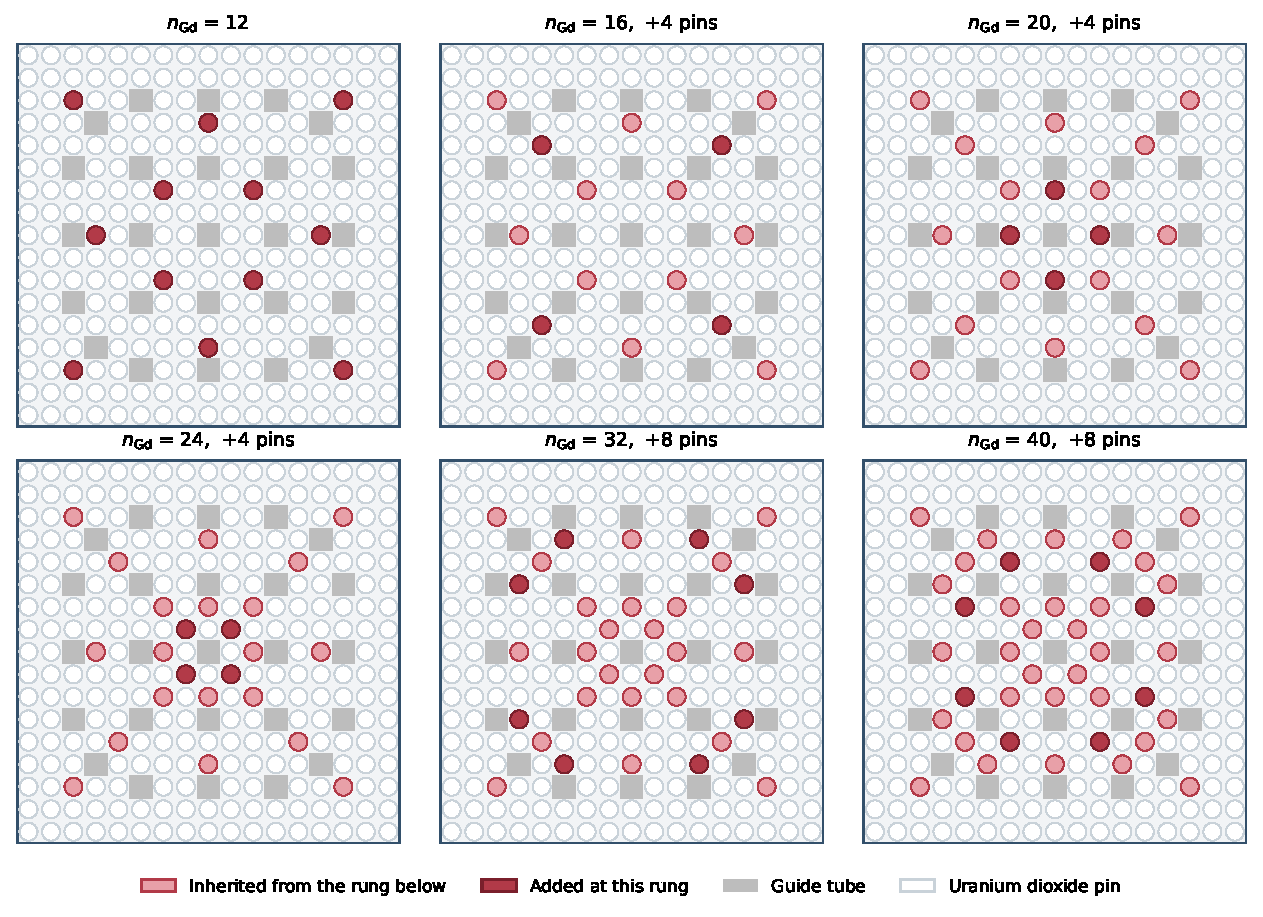
\includegraphics[width=0.92\linewidth]{images/th_gd_ladder.pdf}
  \caption{The six nested poisoned-pin patterns.}
  \label{fig:gd-ladder}
\end{figure}

The rod count is a discrete variable, and it reaches the model in three
steps:

\begin{enumerate}
  \item NSGA-II treats the pin count as a continuous variable inside
        the bounds, so it proposes values such as 13.845.

  \item The evaluator snaps that value to the nearest admissible
        rod count, one of 12, 16, 20, 24, 32 and 40, before the model
        is built, and an exact midpoint is assigned to the lower count.

  \item The archive records both numbers, the value the optimiser
        proposed and the value that was built.
\end{enumerate}

In Campaign 9, for example, the design of index 0 was proposed at
13.845 pins and built with 12, and the design of index 2 was proposed
at 22.446 and built with 24. The positions the added rods take are not free. A gadolinia rod
depresses the thermal flux around itself, so where the rods are placed
changes the assembly peaking factor and the burnout rate of the
absorber at the same rod count. The placement strategy therefore puts
each new rod in the interior of the assembly, around the guide tubes,
following
the optimised 16, 20 and 24 pin maps of Bae, Mertyurek and
Asgari~\cite{bae_gd_2023} and the arrangements of the reference
specification~\cite{nuscale_htp2_2017,epr_fsar_ch4}, under four rules.

\begin{enumerate}
  \item The patterns are nested, so each contains the one below it and
        the twelve-rod heritage arrangement of Campaigns 1 to 4 is the
        smallest of them.
  \item Every pattern is octant-symmetric.
  \item The outer two rod rows are kept absorber free.
  \item Every gadolinia rod is face-adjacent or diagonally adjacent to
        a guide tube, and no two gadolinia rods are face-adjacent to
        each other, which limits mutual shadowing.
\end{enumerate}

\begin{table}[htbp]
  \centering
  \small
  \caption{Constraints: definition and transport model of evaluation.}
  \label{tab:constraints}
\begin{tabularx}{\textwidth}{
    >{\raggedright\arraybackslash}p{0.15\textwidth}
    >{\raggedright\arraybackslash}p{0.40\textwidth}
    >{\raggedright\arraybackslash}X
}
    \toprule
    Constraint & Definition & Evaluated on \\
    \midrule
    $g_{k\min}$ 
        & $1.02 - k_\mathrm{BOL} \le 0$
        & assembly to C5, \textbf{core} from C6 \\

    $g_{k\max}$ 
        & $k_\mathrm{BOL} - k_{\max} \le 0$
        & assembly to C5, \textbf{core} from C6, 
          $k_{\max}$ of Table~\ref{tab:ctrl-bounds} \\

    $g_\mathrm{enr}$ 
        & $e_\mathrm{zoned,max} - e_\mathrm{lim} \le 0$
        & algebraic, $e_\mathrm{lim}$ per campaign \\

    $g_\mathrm{peak}$ 
        & $F_{\Delta H} - 2.0 \le 0$
        & assembly in C1 to C3, \textbf{core} from C4 \\

    $g_\mathrm{geom}$ 
        & $R_\mathrm{env}(p) + \delta + t_\mathrm{refl} + c_\mathrm{v} - 90 \le 0$
        & core, analytic, lattice pad $\delta$ of
          Equation~\eqref{eq:ggeom}, clearance $c_\mathrm{v}$ of 
          Section~\ref{sec:meth-c8-space} \\

    $g_\mathrm{ctrl}$ 
        & $k_\mathrm{RE} - 0.99 \le 0$
        & \textbf{core}, the sixteen regulating-bank assemblies in,
          from C7 \\

    $g_\mathrm{ctrl,12}$ 
        & $k_\mathrm{RE12} - 0.99$
        & core, first two banks in, from C8, 
          \emph{recorded, not constrained} \\
    \bottomrule
\end{tabularx}
\end{table}

The bound of $g_\mathrm{peak}$ takes two values. Campaigns 1 to 8 use
2.0, a deliberately generous adopted value that keeps the exploratory
search free~\cite{epr_fsar_ch4}, and Campaign 9 uses 1.65, the
Technical Specification limit of a licensed pressurised water
reactor~\cite{robinson_gd10}, for the reason given in
Section~\ref{sec:meth-c9}. Satisfying either value is a necessary
condition on a candidate design and not a demonstration of compliance.

\subsection{Geometric feasibility}
\label{sec:meth-geom}

The vessel-fit constraint $g_\mathrm{geom}$ uses the circumscribed
envelope of the intact core footprint.

\begin{equation}
R_\mathrm{env}(p) = \sqrt{13}\,\cdot\,17\,p
\label{eq:renv}
\end{equation}

\noindent where the symbols have the following meaning.

\begin{itemize}
  \item $R_\mathrm{env}$ is the circumscribed radius of the fuel
        region, in cm.

  \item $p$ is the pin pitch, in cm.

  \item $17$ is the number of pin cells per assembly side,
        dimensionless, so that $17p$ is the assembly pitch in cm.

  \item $\sqrt{13} \approx 3.606$ is the dimensionless distance from
        the core centre to the outermost fuel corner of the
        $6\times6$-minus-corners map, in assembly pitches. The extreme
        corner is three assembly pitches along one axis and two along
        the other, so its distance is $\sqrt{3^2 + 2^2} = \sqrt{13}$.
\end{itemize}

The sensitivity of the envelope to the pitch follows directly.

\begin{equation}
\frac{\mathrm{d}R_\mathrm{env}}{\mathrm{d}p} = 61.3~\mathrm{cm\,cm^{-1}}
\label{eq:drenv}
\end{equation}

A pitch increase of one millimetre therefore consumes about
\SI{6.1}{cm} of radial budget. Pitch and reflector thickness compete
directly for the fixed allowance of the 90\,cm vessel internal radius
of Table~\ref{tab:model-geometry}, which makes the two variables
strongly coupled.

The enforced form of the constraint carries two further terms. The
geometry builder pads the lattice corner by a fixed allowance, and
Campaign 8 reserves a clearance for the core barrel and the downcomer.
\begin{equation}
g_\mathrm{geom} \;=\; R_\mathrm{env}(p) \;+\; \delta \;+\;
t_\mathrm{refl} \;+\; c_\mathrm{v} \;-\; R_\mathrm{v} \;\le\; 0
\label{eq:ggeom}
\end{equation}

\noindent where the symbols have the following meaning.

\begin{itemize}
  \item $R_\mathrm{env}(p)$ is the circumscribed radius of
        Equation~\eqref{eq:renv}, in cm.

  \item $\delta$ is the lattice-corner pad of the geometry builder,
        \SI{0.02}{cm}, held in a single constant shared by the builder
        and the constraint.

  \item $t_\mathrm{refl}$ is the reflector thickness, in cm.

  \item $c_\mathrm{v}$ is the reserved barrel and downcomer clearance,
        in cm. It is zero in Campaigns 1 to 7 and \SI{7.08}{cm} in
        Campaigns 8 and 9, as derived in
        Section~\ref{sec:meth-c8-space}. Campaign 9 keeps it, so both
        campaigns search the reflector thickness up to the same
        \SI{5.66}{cm}.

  \item $R_\mathrm{v}$ is the vessel internal radius, \SI{90}{cm}.
\end{itemize}

The pad $\delta$ of \SI{0.02}{cm} is the allowance the geometry builder
adds at the lattice corner so that the outermost pin cells close inside
the core envelope. The builder has applied it from the first campaign.
The analytic constraint did not, up to and including Campaign 4, so the
envelope the optimiser tested was \SI{0.02}{cm} smaller than the one the
code then built.

That difference is only reached by a design whose reflector stands
within \SI{0.02}{cm} of the vessel limit, and the search produces such
designs by construction, since a thicker reflector returns more neutrons
and the optimiser pushes the reflector thickness against its upper bound
wherever reactivity is the binding objective. The first infill batch of
Campaign 4 proposed one, the constraint accepted it, and the geometry
builder could not construct it, so the evaluation failed. The pad is now
a single constant imported by both the constraint and the builder, so
the two descriptions of the same core cannot differ again.

The constraint is tested analytically inside the optimiser, before any
geometry is built, so a design that cannot fit the vessel is rejected
without spending a transport evaluation on it.

\subsection{Eigenvalue model of the reactivity window}
\label{sec:meth-kbasis}

Campaigns 1 to 5 applied the reactivity window to the assembly infinite
multiplication factor. From Campaign 6 both of its bounds act on the
core effective multiplication factor at beginning of life, which the
leakage-corrected target of Section~\ref{sec:meth-ktarget} makes
available at no additional cost, for the reason reported in
Section~\ref{sec:res-c4}. The upper bound is not a constant of this work. It
is the adopted value up to and including Campaign 6 and a
derived quantity from Campaign 7 onwards, so it is written here as a symbol.

\begin{equation}
1.02 \;\le\; k_\mathrm{eff}^\mathrm{core}(\mathbf{x}) \;\le\; k_{\max}
\label{eq:k-window-core}
\end{equation}

\noindent where the symbols have the following meaning.

\begin{itemize}
  \item $k_\mathrm{eff}^\mathrm{core}$ is the effective multiplication
        factor of the 32-assembly core at the beginning of life,
        dimensionless, from the same core solve on which the peaking
        objective is tallied.

  \item $\mathbf{x}$ is the design vector of
        Table~\ref{tab:design-space}.

  \item $k_{\max}$ is the upper reactivity bound of the campaign,
        dimensionless. It is 1.35 through Campaign 6 and takes the
        derived values of Table~\ref{tab:ctrl-bounds} from Campaign 7,
        namely 1.126 in Campaign 7 and 1.166 in Campaigns 8 and 9.
\end{itemize}

The change of basis affects the two bounds differently.

The upper bound keeps the same feasible set. Re-scored on both bases, the
Campaign 5 archive admits the same designs with the core bound at 1.35
as with the assembly bound at 1.40
(Section~\ref{sec:res-c5-kbasis}), so the problem is no looser than
before.

The floor becomes active. The assembly is solved under reflective
boundary conditions, which return every neutron, so its $k_\infty$
carries no leakage and a floor of 1.02 on it rejects almost no design.
The core eigenvalue carries the radial and axial leakage of the whole
core, is therefore several thousand pcm lower for the same design, and
the same floor of 1.02 now rejects the designs that cannot reach
criticality. Campaign 6 shows that happening repeatedly
(Section~\ref{sec:res-c6-doe}).

\subsection{controllability constraint and the upper reactivity bound}
\label{sec:meth-ctrl}

In Campaigns 1 to 6 the upper bound of the reactivity window is an
adopted value of 1.35 and not a controllability criterion.
The transport model of those campaigns carries no control rods, no
rodded state is solved and no bank worth enters the constraint set. The
value bounds the excess reactivity the search may accumulate while the
objective is the cycle length, which is what the exploratory phase
needs.

Controllability is assessed for the first time in the post-analysis of
the Campaign 6 archive, on the first front of this work whose designs
are worth examining as candidates. That assessment produced the
seven-bank scheme of Figure~\ref{fig:cr-banks} and the constraint below,
which enter the constraint set in Campaign 7 under the one-change rule
of Section~\ref{sec:meth-campaigns}.

The constraint replaces the adopted value by a measurement. Every
evaluation of Campaign 7 solves the beginning-of-life core twice, and
every evaluation of Campaigns 8 and 9 three times:

\begin{enumerate}
  \item With every bank withdrawn, which gives the peaking objective
        and the unrodded eigenvalue.

  \item With the four regulating banks inserted, which gives
        $k_\mathrm{RE}$, the eigenvalue the constraint acts on.

  \item From Campaign 8, with the first two regulating banks inserted,
        which gives $k_\mathrm{RE12}$. That reading is recorded and not
        constrained, and it divides the front as described below.
\end{enumerate}

Every assembly of the core carries a control rod assembly, so the
state with all 32 inserted bounds what the control system can hold. The
constraint is conservative with respect to that bound, because it inserts
only the four regulating banks and leaves the shutdown banks
withdrawn.

The banks are those of the seven-bank scheme illustrated in
Figure~\ref{fig:cr-banks}. The scheme was not applied in Campaign 6. It
was defined in the post-analysis of the Campaign 6 archive and entered
the constraint set from Campaign 7, so it governs Campaigns 7, 8 and 9
only. The regulating banks RE1 to RE4
occupy the sixteen central assemblies and carry B$_4$C absorbers. The
shutdown banks occupy the outer sixteen assemblies and stay withdrawn
throughout, because they are reserved for the scram function and a
design that needs them at power is not controllable in normal
operation.

\begin{figure}[htbp]
  \centering
  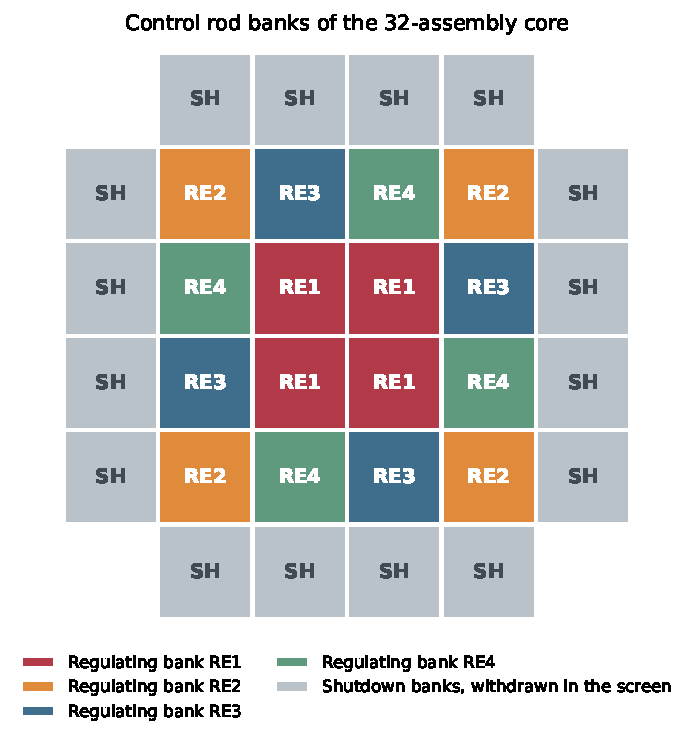
\includegraphics[width=0.62\linewidth]{images/th_cr_banks.pdf}
  \caption{Control rod banks of the 32-assembly core.}
  \label{fig:cr-banks}
\end{figure}

\begin{equation}
k_\mathrm{RE}(\mathbf{x}) = k_\mathrm{eff}^\mathrm{core}\big(\mathbf{x},\ \mathrm{RE1\ to\ RE4\ inserted}\big)
\label{eq:k-re}
\end{equation}

\noindent where the symbols have the following meaning.

\begin{itemize}
  \item $k_\mathrm{RE}$ is the core effective multiplication factor at
        beginning of life with the sixteen regulating-bank assemblies
        inserted and the sixteen shutdown-bank assemblies withdrawn,
        dimensionless.

  \item $\mathbf{x}$ is the design vector.
\end{itemize}

The constraint demands an operating subcriticality margin.

\begin{equation}
g_\mathrm{ctrl}(\mathbf{x}) = k_\mathrm{RE}(\mathbf{x}) - (1 - \Delta\rho_\mathrm{op}) \le 0
\label{eq:g-ctrl-meth}
\end{equation}

\noindent where the symbols have the following meaning.

\begin{itemize}
  \item $g_\mathrm{ctrl}$ is the constraint value, dimensionless,
        negative when satisfied.

  \item $\Delta\rho_\mathrm{op}$ is the operating margin, \num{0.01} in
        units of $k$, that is \SI{1000}{pcm}.
\end{itemize}

The worth of the regulating banks is read from the same pair of solves.

\begin{equation}
\rho_\mathrm{bank}(\mathbf{x}) = k_\mathrm{eff}^\mathrm{core}(\mathbf{x}) - k_\mathrm{RE}(\mathbf{x})
\label{eq:bank-worth}
\end{equation}

\noindent where the symbols have the following meaning.

\begin{itemize}
  \item $\rho_\mathrm{bank}$ is the worth of the sixteen regulating-bank
        assemblies, in units of $k$, reported in pcm after
        multiplication by $10^5$.

  \item $k_\mathrm{eff}^\mathrm{core}$ is the unrodded core effective
        multiplication factor at beginning of life, dimensionless.
\end{itemize}

The margin is a modelling choice. An insertion of the regulating banks
alone with a \SI{1000}{pcm} margin is not a licensing shutdown
margin. The constraint
therefore tests whether the regulating system can hold the fresh core
subcritical at power conditions, which is the question the reactivity
bound was standing in for.

Two further rodded states appear in this work, and neither is
constrained. The state $k_\mathrm{RE12}$ inserts only the eight
assemblies of banks RE1 and RE2, the four central assemblies and the
four diagonal assemblies of the middle ring. It is recorded from
Campaign 8 as $g_\mathrm{ctrl,12}$, so that the post-analysis can
divide the front into designs controllable with two banks and designs
that need all four. The margins $M_{16}$ and $M_{8}$ of
Table~\ref{tab:c8-post-boron} are those of the sixteen- and of the
eight-assembly insertion. Neither is a margin of the all-rods-in state,
which inserts all 32 control rod assemblies and therefore includes the
sixteen shutdown-bank assemblies that this work keeps
withdrawn.

The upper reactivity bound of $g_{k\max}$ can now be derived from the
measured bank worth rather than adopted.

\begin{equation}
k_{\max} = (1 - \Delta\rho_\mathrm{op}) + \min_{\mathbf{x} \in \mathcal{S}} \rho_\mathrm{bank}(\mathbf{x})
\label{eq:k-max-derived}
\end{equation}

\noindent where the symbols have the following meaning.

\begin{itemize}
  \item $k_{\max}$ is the derived bound on the unrodded core
        eigenvalue, dimensionless.

  \item $\rho_\mathrm{bank}$ is the bank worth, the difference between
        the unrodded and the rodded eigenvalues, dimensionless.

  \item $\mathcal{S}$ is the sample of designs on which the worth was
        measured.
\end{itemize}

Table~\ref{tab:ctrl-bounds} lists the bounds used and derived. Its
three-dimensional values come from the axial study of
Section~\ref{sec:meth-lax}.

\begin{table}[htbp]
  \centering
  \caption{Upper reactivity bounds by campaign and their provenance.}
  \label{tab:ctrl-bounds}
  \small
  \begin{tabularx}{\textwidth}{@{}>{\raggedright\arraybackslash}p{0.16\textwidth}c>{\raggedright\arraybackslash}p{0.20\textwidth}>{\raggedright\arraybackslash}X@{}}
    \toprule
    Campaigns & $k_{\max}$ & Basis & Provenance \\
    \midrule
    C1 to C6 & 1.35  & assembly, then core & adopted value \\
    retrospective & 1.368 & core, 2D & all seven banks, \SI{1000}{pcm}, eight C6 designs \\
    C7 & 1.126 & core, 2D & four regulating banks, eight C6 designs, worths \num{12174} to \SI{12718}{pcm} \\
    C7 measured & 1.099 to 1.217 & core, 2D & implied by each design's own worth, 60 designs \\
    C8 and C9 & 1.166 & core, 2D from 3D & smallest 3D worth \SI{14307}{pcm}, times $L_\mathrm{ax}$ \\
    \bottomrule
  \end{tabularx}
\end{table}

A bound derived this way has two weaknesses. The minimum of a small
sample is a biased estimate of the minimum of the population, and the
quantity it stands in for is measured on every evaluation from Campaign
7. From Campaign 8 the measured constraint therefore decides feasibility,
and the derived value is kept only as a outer bound
(Section~\ref{sec:res-c7-screens}).

The retrospective value of 1.368, derived from the worth of all 32
control rod assemblies with the same margin, is two per cent above the
adopted 1.35, which is therefore the all-bank controllability bound of
this core to within that tolerance.


\subsection{Objective functions}
\label{sec:objective_functions}

\subsubsection{Cycle length}

The cycle length is an objective in Campaigns 1 to 8 and a constraint in
Campaign 9, where the five-year requirement enters
Equation~\eqref{eq:c9-problem}. It is computed in the same way in both
cases, from the end-of-cycle burnup through the conversion of
Equation~\eqref{eq:efpd}, with the specific power of
Table~\ref{tab:model-operating}. What remains to be fixed here is the
criterion that defines the end of cycle on the model used for the
depletion, the reflective single assembly.

\begin{equation}
B_\mathrm{EOC} = \min\!\left( B_k,\, B_\mathrm{burnup} \right)
\label{eq:eoc}
\end{equation}

\begin{equation}
B_k = \min\left\{\, B > 0 \,:\, k_\infty(B) \le k_\mathrm{target} \,\right\}
\label{eq:eoc-k}
\end{equation}

\noindent where the symbols have the following meaning.

\begin{itemize}
  \item $B_\mathrm{EOC}$ is the end-of-cycle burnup entering
        Equation~\eqref{eq:efpd}, in MWd/kgHM.

  \item $B_k$ is the reactivity-defined end-of-cycle burnup, in
        MWd/kgHM.

  \item $B_\mathrm{burnup}$ is the discharge-burnup limit, equal to
        55\,MWd/kgHM on the assembly-average basis, with its basis and
        its relation to the depletion horizon in
        Section~\ref{sec:meth-atf}.

  \item $B$ is the burnup along the depletion history, in MWd/kgHM.

  \item $k_\infty(B)$ is the infinite multiplication factor of the
        reflective assembly at burnup $B$, dimensionless.

  \item $k_\mathrm{target}$ is the leakage-corrected end-of-cycle
        target, dimensionless, defined in
        Section~\ref{sec:meth-ktarget}.
\end{itemize}

The crossing $B_k$ is obtained by linear interpolation between the two
consecutive depletion steps between which the residual
$k_\infty - k_\mathrm{target}$ changes sign.

The depletion terminates adaptively, at the first step below the
target, and this forces it to advance in short blocks. The solver requires its complete step list before the
calculation starts, while the stopping burnup is a property of the
design being evaluated and is not known in advance. Each block is
therefore a separate depletion call that restarts from the results
file written by the previous one, and a restart requires that file to
carry both the material composition and the reaction rates.

\label{sec:restart_defect}%
The depletion solver of OpenMC~0.15.3, the version used in this work,
writes no reaction rates to its results files unless the
\texttt{write\_rates} option of the integrator is set, and its default
is false. A restart from a
results file that carries no reaction rates advances its first step
with every transmutation channel set to zero, so the fuel evolves by radioactive decay alone
while the burnup label advances by the full step. The failure is
silent, because the calculation completes and every value it returns
is of a plausible magnitude. The evaluator therefore now requests the
rates explicitly at every block and refuses to restart from a file
that carries none.

That guard entered the evaluator in Campaign 6. A campaign is exposed
to the defect only where it restarts, so Campaign 1 is unaffected, its
fixed schedule completing in a single depletion call, and from Campaign
6 the rates are requested at every block and the recorded burnup agrees
with the physical one.

The histories of Campaigns 3 to 5, which are the campaigns run with
the adaptive schedule whose cycle lengths enter the results of this
work, were corrected without repeating any depletion, and every
affected cycle length is corrected before use.
The correction was verified by depleting one design twice with the same
seed, once as a single block and once in three blocks, which reproduced
an offset of exactly one step per restart. Its size on the affected
archives is reported in Section~\ref{sec:res-c5-c7}. The compositions
computed at every step are physically correct. Only the burnup labels
are wrong, because every restart advanced the label by one full step in
which the fuel did not burn. The correction is applied to the archived
histories in two steps:

\begin{enumerate}
  \item The first point of every restarted block is discarded, because
        it repeats the state that precedes it.

  \item The remaining points are relabelled by subtracting the burnup
        of every step lost at a restart.
\end{enumerate}

The relabelling is given by Equation~\eqref{eq:true_burnup}.

\begin{equation}
B_\mathrm{true} = B_\mathrm{label} - \sum_{j=1}^{n_\mathrm{r}} \Delta b_j
\label{eq:true_burnup}
\end{equation}

\noindent where the symbols have the following meaning.

\begin{itemize}
  \item $B_\mathrm{label}$ is the cumulative burnup recorded by the
        evaluator, in MWd/kgHM.

  \item $B_\mathrm{true}$ is the burnup physically reached by the fuel,
        in MWd/kgHM.

  \item $n_\mathrm{r}$ is the number of restarted blocks,
        dimensionless.

  \item $\Delta b_j$ is the first step of the $j$-th restarted block,
        lost to the defect, in MWd/kgHM. It equals the marching step of
        \SI{4.0}{\mega\watt\day\per\kilo\gram} unless the depletion horizon
        leaves less.
\end{itemize}

The first block, which ends at \SI{13.5}{\mega\watt\day\per\kilo\gram},
contains no restart and is unaffected. For blocks of two equal steps the
correction halves the burnup accumulated after the first block. A final block truncated at the
depletion horizon carries fewer steps than the others, and the burnup it
loses is still that of one full step.


\subsubsection{Radial peaking factor}
\label{sec:meth-fdh}

The peaking objective of Equation~\eqref{eq:obj_fdh} uses the radial
peaking factor of Equation~\eqref{eq:fdh_definition}, formally defined
in Section~\ref{sec:bg-peaking}. That definition leaves two
methodological choices open, and both are fixed here:

\begin{itemize}
  \item \textbf{Numerical estimator:} the integrals of
        Equation~\eqref{eq:fdh_definition} are replaced by
their Monte Carlo counterparts. A pin-wise fission energy deposition
tally is accumulated over the active fuel region, so each rod
contributes one volume-integrated score.

\begin{equation}
\widehat{F}_{\Delta H}
=
\frac{\displaystyle \max_{i \in \{1,\dots,N\}} \widehat{P}_i}
     {\displaystyle \frac{1}{N} \sum_{j=1}^{N} \widehat{P}_j}
\label{eq:fdh_estimator}
\end{equation}

\noindent where the symbols have the following meaning.

\begin{itemize}
  \item $\widehat{F}_{\Delta H}$ is the Monte Carlo estimate of the
        radial peaking factor, dimensionless.

  \item $\widehat{P}_i$ is the tallied fission energy deposition rate
        of fuel rod $i$ over the full active height, in W.

  \item $N$ is the number of fuel rods in the evaluation domain,
        dimensionless.

  \item $i$ and $j$ are fuel rod indices, dimensionless.
\end{itemize}

Two properties of this estimator govern the selection methodology.

\begin{enumerate}
  \item The estimate carries a statistical uncertainty inherited from
        the finite number of simulated histories. Differences between
        candidate designs smaller than that uncertainty cannot be
        resolved by a single evaluation.

  \item The estimate is positively biased. The numerator is the
        maximum over the scores of $N$ fuel rods, each carrying its own
        statistical fluctuation, so fluctuation alone raises the sampled
        maximum above the true maximum. The bias decreases as the
        number of simulated histories increases, because the tally
        variance decreases with it.
\end{enumerate}

  \item \textbf{Evaluation domain:} the tally domain of
        Equation~\eqref{eq:fdh_estimator} determines what the objective
        represents. Two levels are used in this work.

\begin{enumerate}
  \item Assembly level, in which $N$ covers the 264 fuel rods of a
        single reflected assembly. This level is inexpensive and was the
        tally domain of the peaking objective in Campaigns 1 to 3.

  \item Core level, in which $N$ covers the fuel rods of the full
        32-assembly core at beginning of life. This level is the tally
        domain of both the objective and the peaking constraint from
        Campaign 4 onward.
\end{enumerate}
\end{itemize}

Every campaign solve of this work, at assembly and at core level, is
two-dimensional: an axial segment of the lattice bounded above and
below by reflective boundaries. The fission energy
deposition rate of a rod is then uniform along $z$, so the integral of
Equation~\eqref{eq:fdh_definition} is $q'_i H$ for every rod $i$ with
the same $H$, and that common factor cancels between the numerator and
the denominator. What the tally returns for each rod, the fission
energy deposition rate integrated over the segment, is therefore already
proportional to the height-integrated quantity that
Equation~\eqref{eq:fdh_definition} requires, and
Equation~\eqref{eq:fdh_estimator} is formed from those scores directly.

The two-dimensional value equals the three-dimensional one only if the
power distribution is separable, that is if the power of rod $i$ at
elevation $z$ can be written as a radial factor times an axial shape
that is the same for every rod.

A reflective boundary returns every neutron that reaches it along the
mirrored direction~\cite{openmc_docs}, which makes the segment
equivalent to an axially infinite medium. The axial leakage is
therefore zero and the geometry is invariant under translation in $z$.
The flux of such a medium carries no spatial dependence along the
direction of the
reflection~\cite{duderstadt_hamilton_1976}, so the axial power shape
satisfies a condition stronger than separability: it is not only the
same for every rod, it is constant, and $q'_i(z) = q'_i$ for every rod
$i$ and every elevation $z$. Separability is therefore not an
approximation of the two-dimensional model but a property of its
boundary condition, and the $z$ dependence that
Equation~\eqref{eq:fdh_definition} integrates over is absent from the
calculation.

A core of finite height breaks that symmetry, because it has a top and
a bottom. Three features of it make the axial shape depend on which rod
is examined.

\begin{itemize}
  \item \textbf{Axial leakage:} the axial reflector returns neutrons at
        the top and the bottom, and the amount returned depends on the
        radial position of the rod, so the axial shape of a peripheral
        rod is flatter than that of a central one.

  \item \textbf{Spacer grids:} each grid is a local absorber at a fixed
        elevation, and its depression of the flux scales with the local
        thermal flux, which varies radially.

  \item \textbf{Inserted rods:} a partially inserted bank absorbs over
        part of the height only, so the axial shape of a rod next to an
        inserted guide tube differs from that of a rod far from one.
\end{itemize}

The height integral of a rod is then no longer a common multiple of its
mid-plane rate, and the two estimators differ. The size of that
difference on the candidate designs is measured in
Section~\ref{sec:res-c9-peaking}.

The assembly estimator is in turn a poor predictor of the core value,
which is what moved the tally domain to core level from Campaign 4. The
study that established this is described in
Section~\ref{sec:meth-core-objective} and its measurements are reported
in Section~\ref{sec:res-corevalidation}.

\subsubsection{Normalisation of the constraint violation}
\label{subsubsec:cv-norm}

The constraints of the problem carry five different units.

\begin{enumerate}
  \item The multiplication factor, in units of $k$, for the reactivity
        window $g_{k\min}$ and $g_{k\max}$ and for the controllability
constraints $g_\mathrm{ctrl}$ and $g_\mathrm{ctrl,peak}$.

  \item The weight percentage for the enrichment limit
        $g_\mathrm{enr}$.

  \item A dimensionless power ratio for the peaking limit
        $g_\mathrm{peak}$.

  \item The centimetre for the vessel-fit condition
        $g_\mathrm{geom}$.

  \item The day for the cycle-length floor of Campaign 9,
        $g_\mathrm{efpd}$.
\end{enumerate}

When no member of the population is feasible,
NSGA-II ranks the candidates by their total constraint violation, and a
sum of raw violations weights each constraint by its unit. A vessel-fit
violation of \SI{1}{cm} contributes 1.0 to the sum, ten times the
contribution of a reactivity violation of \SI{10000}{pcm}, which is 0.1
in units of $k$.

From Campaign 6 onward, each constraint is divided by a scale before it
enters the optimiser.

\begin{equation}
  V = \sum_{j=1}^{n_g} \max\!\left(0, \frac{g_j}{s_j}\right)
  \label{eq:cv-norm}
\end{equation}

The terms of Equation~\eqref{eq:cv-norm} have the following meaning.

\begin{itemize}
  \item $V$ is the total constraint violation used to rank infeasible
    candidates, dimensionless.
  \item $g_j$ is the raw value of constraint $j$ in its native unit, with
    $g_j \leq 0$ denoting feasibility.
  \item $s_j$ is the normalisation scale of constraint $j$, taken equal to the
    limit of that constraint, in the same unit as $g_j$.
  \item $n_g$ is the number of inequality constraints, dimensionless.
\end{itemize}

Each scale is the limit of its constraint in the campaign concerned,
and Table~\ref{tab:cv-scales} gives the values with the sections that
derive them. The controllability constraints are the exception, since their
limit is 0.99 while the scale is the critical value of 1.0.

\begin{table}[htbp]
  \centering
  \small
  \caption{Normalisation scales $s_j$ of the constraint violation, Campaigns 6 to 9.}
  \label{tab:cv-scales}
  \begin{tabular}{@{}l l r r r r@{}}
    \toprule
    Constraint & Unit of $g_j$ & C6 & C7 & C8 & C9 \\
    \midrule
    $g_{k\min}$            & $\Delta k$ & 1.02  & 1.02  & 1.02  & 1.02  \\
    $g_{k\max}$            & $\Delta k$ & 1.35  & 1.126 & 1.166 & 1.166 \\
    $g_\mathrm{enr}$       & wt\%       & 19.75 & 12    & 16    & 16    \\
    $g_\mathrm{peak}$      & --         & 2.0   & 2.0   & 2.0   & 1.65  \\
    $g_\mathrm{geom}$      & cm         & 90.0  & 90.0  & 82.92 & 82.92 \\
    $g_\mathrm{ctrl}$      & $\Delta k$ & --    & 1.0   & 1.0   & 1.0   \\
    $g_\mathrm{ctrl,peak}$ & $\Delta k$ & --    & --    & --    & 1.0   \\
    $g_\mathrm{efpd}$      & days       & --    & --    & --    & 1826  \\
    \bottomrule
  \end{tabular}
\end{table}

The normalisation preserves the sign of every $g_j$, so the feasible set
is unchanged. It acts on the constraint matrix only, so the objectives
and the hypervolume history are unchanged. The archived constraint
values are stored unscaled and normalised when the archive is loaded.
The active scales are written into the checkpoint metadata, and a
resumed campaign does not start if its constraint set differs from the
stored one.

Division by the limit gives every constraint the same weight per unit of
relative exceedance. The weighting orders the infeasible designs only,
because NSGA-II ranks every feasible design above every infeasible one,
and the reported Pareto fronts, which contain feasible designs only, do
not depend on it.

\section{Campaign structure: one change per campaign}
\label{sec:meth-campaigns}

Each campaign changes \emph{one} thing relative to its predecessor, so
every observed difference is attributable
(Table~\ref{tab:campaigns}).

\begin{table}[htbp]
  \centering
  \small
  \caption{Campaign structure.}
  \label{tab:campaigns}
  \begin{tabularx}{\textwidth}{@{}cc>{\raggedright\arraybackslash}X@{}}
    \toprule
    Campaign & Evaluations & Change relative to the previous campaign \\
    \midrule
    C1 & 72  & None, verification run \\
    C2 & 84  & Analytic vessel-fit constraint $g_\mathrm{geom}$ \\
    C3 & 72  & Fidelity study, per-design seeds, in-loop burnup limit \\
    C4 & 54  & $F_{\Delta H}$ and $g_\mathrm{peak}$ evaluated on the core \\
    C5 & 60  & Gadolinia rod count as a design variable \\
    C6 & 114 & Three bundled corrections, then one acquisition change per block \\
    C7 & 60  & Measured controllability constraint $g_\mathrm{ctrl}$ \\
    C8 & 60  & Fixed pitch, single enrichment, axial-corrected target, two-level constraint \\
    C9 & 60  & Objectives $F_{\Delta H}$ and $c_\mathrm{max}$, cycle length as a constraint \\
    \bottomrule
  \end{tabularx}
\end{table}

Campaign 6 is the only campaign that changes more than one element of
the problem. It applies together three corrections established by the
Campaign 5 analyses. Each was necessary for a usable Pareto front, and
each acts on a separate output of the evaluator, so its effect remains
attributable:

\begin{enumerate}
  \item \textbf{Eigenvalue model:} the reactivity window is evaluated
        on the core $k_\mathrm{eff}$ instead of the assembly $k_\infty$
        (Section~\ref{sec:meth-kbasis}). The change acts only on the
        feasibility classification, and its effect was quantified on the
        Campaign 4 and Campaign 5 archives before the campaign was
        launched (Section~\ref{sec:res-c5-c7}).

  \item \textbf{Radial zoning:} the enrichment map of the
        beginning-of-life core is zoned inside the evaluator
        (Section~\ref{sec:meth-zoning}), which flattens the radial power
        distribution. It entered after Campaign 5, in response to the
        peaking violations that the Campaign 4 and Campaign 5 archives
        show on the core basis (Section~\ref{sec:res-c4}). The zoning
        acts only on beginning-of-life core quantities, while the cycle
        length comes from the depletion of the unzoned reflective
        assembly, so it cannot change the cycle length.

  \item \textbf{Depletion horizon:} the horizon is raised to
        $B_\mathrm{max} = \SI{100}{MWd/kgHM}$
        (Section~\ref{sec:meth-atf}). The previous horizon stopped the
        depletion before those designs reached the target, so each was
        recorded with the same cycle length, a lower bound on the value
        the design would have reached, and the optimiser could not rank
        them. Such an observation is right-censored, and the term is
        used in that sense throughout this work. The horizon changes only the designs that
        reach the old horizon before the target
        (Section~\ref{sec:res-c5-c7}).
\end{enumerate}

Testing the three corrections one campaign at a time would have required
three further campaigns of about 60 transport evaluations each. The
one-change rule is instead kept inside the campaign, where each of the
four infill blocks changes one element of the acquisition function of
Section~\ref{sec:meth-acq} (Section~\ref{sec:res-c6}).

Campaign 9 changes the formulation, and four settings follow from it
(Section~\ref{sec:meth-c9}).

\begin{enumerate}
  \item The cycle length becomes a constraint.

  \item The critical soluble boron concentration at the reactivity
        maximum becomes a measured objective.

  \item The controllability constraint is applied at the operating maximum
        as well as at beginning of life.

  \item The peaking constraint is tightened from 2.0 to 1.65.
\end{enumerate}

The comparison with Campaign 8 is reported design by design in
Section~\ref{sec:res-c9-compare}.

\section{Design space and formulation of Campaigns 8 and 9}
\label{sec:meth-c8-space}

Campaigns 8 and 9 are the two campaigns in which no new defect of the
model or of the loop was found, and their Pareto fronts are the
candidate results of this work. Campaign 8 narrows the design space
with what the earlier campaigns measured, removing from the search the
regions they showed to return infeasible designs, so that the
evaluation budget is spent where feasible designs exist. Campaign 9
keeps that design space and changes the formulation of the problem.
Table~\ref{tab:c89-spec} sets the two side by side.

\begin{table}[htbp]
  \centering
  \small
  \caption{Campaigns 8 and 9: design space and formulation.}
  \label{tab:c89-spec}
  \begin{tabular}{@{}l l l@{}}
    \toprule
    Item & Campaign 8 & Campaign 9 \\
    \midrule
    Enrichment $e$                 & 3.0 to \SI{13.913}{wt\%} & 2.0 to \SI{13.913}{wt\%} \\
    Gadolinia fraction $w_\mathrm{Gd}$ & 0 to \SI{8.0}{wt\%}  & 0 to \SI{8.0}{wt\%} \\
    Reflector thickness $t_\mathrm{refl}$ & 2.0 to \SI{5.66}{cm} & 2.0 to \SI{5.66}{cm} \\
    Gadolinia rods $n_\mathrm{Gd}$ & discrete, 12 to 40     & discrete, 12 to 40 \\
    Pin pitch                      & fixed, \SI{1.26}{cm}   & fixed, \SI{1.26}{cm} \\
    Clearance $c_\mathrm{v}$       & \SI{7.08}{cm}          & \SI{7.08}{cm} \\
    \midrule
    Objectives                     & max EFPD, min $F_{\Delta H}$ & min $F_{\Delta H}$, min $c_\mathrm{max}$ \\
    Cycle length                   & objective              & constraint, $\ge 1826$ EFPD \\
    Peaking bound                  & 2.0                    & 1.65 \\
    Controllability                & beginning of life      & beginning of life and operating maximum \\
    \midrule
    Evaluations                    & 36 + $4\times6$ = 60   & 24 + $6\times6$ = 60 \\
    \bottomrule
  \end{tabular}
\end{table}

\subsection{Design space}

Four decisions define the design space of Campaign 8, and Campaign 9
changes only the lower enrichment bound:

\begin{enumerate}
  \item The pin pitch is fixed at \SI{1.26}{cm}, the rod pitch of the
        Westinghouse $17\times17$ assembly~\cite{todreas_kazimi_2012}
        and of the NuScale fuel assembly~\cite{nuscale_htp2_2017}, which
        the reference fuel design of Section~\ref{sec:design-basis}
        already adopts. Three findings led to this decision.

        \begin{itemize}
          \item Below \SI{1.224}{cm} the lattice clips the guide-tube
                wall at the cell
                boundary without a warning from the code. At the lower
                pitch bound of \SI{1.150}{cm} up to \SI{28}{\%} of the
                wall is replaced by moderator
                (Figure~\ref{fig:gt-clip}). Twenty-five of the 60
                Campaign 7 designs, and designs of every earlier
                campaign, are in this range
                (Section~\ref{sec:res-c7-limits}).

\begin{figure}[htbp]
  \centering
  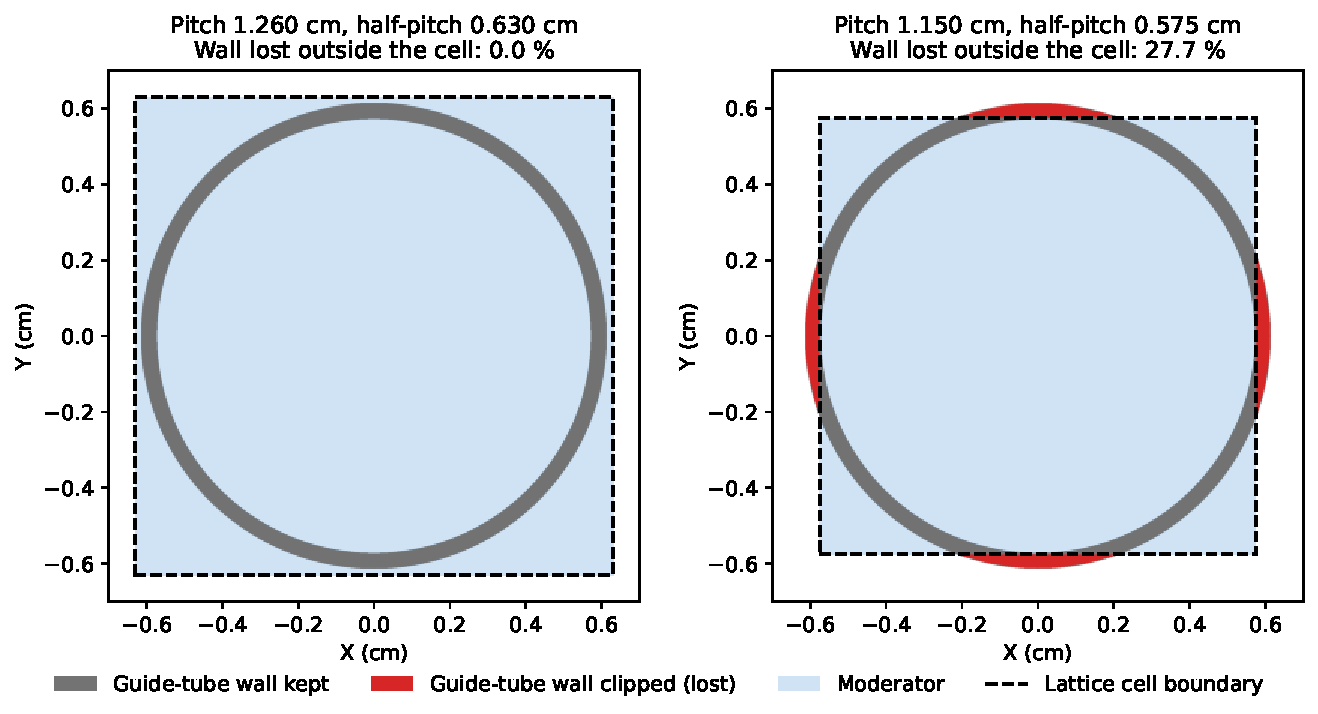
\includegraphics[width=0.75\linewidth]{images/th_gt_clip.pdf}
  \caption{Guide-tube wall and lattice cell at the reference pitch and at the lower pitch bound.}
  \label{fig:gt-clip}
\end{figure}


          \item The pitch is the design variable with the largest
                effect on the regulating-bank worth
                (Section~\ref{sec:res-c7-worth}).

          \item The pitch sets the moderator-to-fuel ratio, on which the
                moderator temperature coefficient
                depends~\cite{duderstadt_hamilton_1976}, and the coolant
                flow area and pressure drop~\cite{todreas_kazimi_2012}.
                The model has no thermal-hydraulic feedback, so it cannot
                itself show whether a given pitch is coolable. The pitch
                is therefore fixed at \SI{1.26}{cm}, the value of the
                operating $17\times17$ lattice, whose thermal-hydraulic
                performance over the enrichment range searched here is
                demonstrated by decades of service in commercial
                PWRs and documented in their
                safety analysis
                reports~\cite{epr_fsar_ch4,todreas_kazimi_2012}.
        \end{itemize}

  \item The two assembly enrichment zones collapse to one variable,
        since the core-level enrichment variation comes entirely from
        the ring multipliers of Section~\ref{sec:meth-zoning}. Its
        upper bound is \SI{13.913}{wt\%}, the value that holds the
        as-built peripheral ring at its own limit through
        Equation~\eqref{eq:leu-box}, so no proposed design can violate
        $g_\mathrm{enr}$.

  \item The vessel-fit constraint reserves a clearance
        $c_\mathrm{v} = \SI{7.08}{cm}$ for a core barrel and a
        downcomer: the \SI{5.08}{cm} stainless steel barrel of the
        reference specification and a \SI{2.0}{cm} downcomer, adopted
        as a minimum coolant return path. The clearance acts on the
        geometric constraint alone, since the campaign transport model
        keeps a vacuum boundary at the reflector surface
        (Section~\ref{sec:meth-barrel}).

  \item The reflector thickness is bounded by the radial budget that
        remains, Equation~\eqref{eq:refl-budget-c8}.
\end{enumerate}

\begin{equation}
t_\mathrm{refl}^{\max} = R_\mathrm{v} - c_\mathrm{v} - R_\mathrm{env}(p) - \delta
\label{eq:refl-budget-c8}
\end{equation}

\noindent where the symbols have the following meaning.

\begin{itemize}
  \item $t_\mathrm{refl}^{\max}$ is the largest reflector thickness that
        fits, \SI{5.669}{cm}, bounded in the design space at
        \SI{5.66}{cm} so that the box edge is strictly feasible.

  \item $R_\mathrm{v}$ is the vessel internal radius, \SI{90}{cm}.

  \item $c_\mathrm{v}$ is the reserved clearance, \SI{7.08}{cm}.

  \item $R_\mathrm{env}(p)$ is the circumscribed radius of the
        32-assembly fuel envelope at pitch $p$, \SI{77.231}{cm} at
        \SI{1.26}{cm}.

  \item $\delta$ is the lattice pad, \SI{0.02}{cm}.
\end{itemize}

Fixing the pitch has a cost that was known before the campaign, since
the designs of lowest peaking in Campaign 7 reach it with thick
reflectors that fit only at a narrow pitch and cannot be built at
\SI{1.26}{cm} (Section~\ref{sec:res-c5-c7}). Campaign 8 therefore
trades the minimum $F_{\Delta H}$ of Campaign 7 for a geometrically
valid lattice.

Both campaigns run the acquisition function of
Section~\ref{sec:meth-acq} at the two settings established in Campaign
6.

\begin{itemize}
  \item \textbf{Batch diversity distance:} $\delta_\mathrm{min} = 0.14$,
        the minimum normalised distance that separates any two designs
        of an infill batch. It acts on the selection of the batch and
        not on the constraints.

  \item \textbf{Feasibility margin coefficient:} $\kappa = 1.5$, the
        number of predictive standard deviations of the constraint
        surrogates that a candidate must hold in reserve to be ranked
        as margin-feasible.
\end{itemize}

Both are passed explicitly to the launcher after the Campaign 7
regression, in which the default values were used instead.

\subsection{Campaign 9 formulation}
\label{sec:meth-c9}

Campaigns 1 to 8 maximise the cycle length. In Campaign 8 every front
design has a cycle length well above the reported refuelling interval,
and the beginning-of-life excess reactivity that this cycle requires
can only be compensated by a deep insertion of the regulating banks
(Section~\ref{sec:res-c8-mission}). Campaign 9 therefore imposes the
required cycle length as a constraint and replaces it as an objective
by $c_\mathrm{max}$, the critical soluble boron concentration at the
reactivity maximum of the cycle. Minimising $c_\mathrm{max}$ directs the
search toward designs whose excess reactivity is held down by the
burnable absorbers rather than by the coolant, so the objective
measures how far each design stands from soluble-boron-free operation.

Campaign 9 takes the five-year refuelling interval reported for the
prototype~\cite{dinizcosta_2017} as the mission requirement, which
gives the floor of 1826 effective full power days used below.

\begin{equation}
\begin{aligned}
\min_{\mathbf{x}}\ &\big(F_{\Delta H}(\mathbf{x}),\ c_\mathrm{max}(\mathbf{x})\big) \\
\text{subject to}\ &\mathrm{EFPD}(\mathbf{x}) \ge 1826,\quad
F_{\Delta H}(\mathbf{x}) \le 1.65,\quad g_j(\mathbf{x}) \le 0
\end{aligned}
\label{eq:c9-problem}
\end{equation}

\noindent where the symbols have the following meaning.

\begin{itemize}
  \item $F_{\Delta H}$ is the radial peaking factor of the zoned core
        with all rods out at beginning of life, the objective of
        Campaign 8, dimensionless.

  \item $c_\mathrm{max}$ is the critical boron concentration at the
        operating maximum of the reactivity history, in ppm, defined in
        Equation~\eqref{eq:c9-cmax}.

  \item $\mathrm{EFPD}$ is the cycle length of
        Section~\ref{sec:objective_functions}.

  \item $1.65$ is the peaking constraint, reduced from the exploratory
        bound of 2.0 of Table~\ref{tab:constraints} to the Technical
        Specification limit of 1.65 of a licensed pressurised water
        reactor~\cite{robinson_gd10}.

  \item $g_j$ are the constraints $g_{k\min}$, $g_{k\max}$,
        $g_\mathrm{enr}$ and $g_\mathrm{geom}$ of
        Table~\ref{tab:constraints} with their Campaign 8 values, the
        controllability constraint $g_\mathrm{ctrl}$ at beginning of life, and the
        same constraint evaluated at the operating maximum,
        $g_\mathrm{ctrl,peak}$.
\end{itemize}

The critical concentration is computed inside the evaluator from
unrodded core solves at 1000, 2000 and, where the reactivity has not
yet changed sign, \SI{3000}{ppm}. The beginning-of-life concentration
$c_\mathrm{BOL}$ is the root of $\rho(c)$, found by interpolation
over the interval between the two solves across which $\rho(c)$
changes sign, or by extrapolation above the highest,
and the differential worth is its local slope at that root. The
concentration at the operating maximum adds the part of the gadolinium
hump that the boron has to hold, measured on the assembly depletion
history as a difference of reactivity.

\begin{equation}
\Delta\rho_\mathrm{hump} = \rho(k_\mathrm{peak}) - \rho(k_\mathrm{BOL}),
\qquad \rho(k) = 10^5\,\frac{k-1}{k}
\label{eq:c7-hump}
\end{equation}

\noindent where the symbols have the following meaning.

\begin{itemize}
  \item $\Delta\rho_\mathrm{hump}$ is the hump, in pcm. It is negative
        when beginning of life is the most reactive state of the design.

  \item $k_\mathrm{BOL}$ is the assembly $k_\infty$ at zero burnup,
        xenon-free, at \SI{1000}{ppm}, dimensionless.

  \item $k_\mathrm{peak}$ is the largest assembly $k_\infty$ over the
        operating points of the depletion history after beginning of
        life, dimensionless.

  \item $\rho$ is the reactivity, in pcm.
\end{itemize}

The concentration at the operating maximum then follows.

\begin{equation}
c_\mathrm{max} = c_\mathrm{BOL} + \frac{\max\!\big(L\,\Delta\rho_\mathrm{hump},\ 0\big)}{w_\mathrm{B}}
\label{eq:c9-cmax}
\end{equation}

\noindent where the symbols have the following meaning.

\begin{itemize}
  \item $c_\mathrm{BOL}$ is the critical boron concentration at
        beginning of life, in ppm.

  \item $\Delta\rho_\mathrm{hump}$ is the hump of
        Equation~\eqref{eq:c7-hump}, taken from the xenon-free assembly
        depletion history that the evaluator already computes, in pcm.
        A hump below \SI{400}{pcm} is set to zero. That floor is twice
        the seed-to-seed standard deviation of the hump at the
        Campaign 9 transport setting of $4\,000\times60$, which the
        seed-replicated study of
        Section~\ref{sec:res-c9-dep-check} measures at \SI{217}{pcm}, so
        a hump below it is not resolved by a single evaluation.

  \item $L$ is the ratio of the assembly to the core beginning-of-life
        eigenvalue of the same design, which carries the assembly hump
        to the core, dimensionless.

  \item $w_\mathrm{B}$ is the differential boron worth at the root, in
        pcm per ppm.
\end{itemize}

Two guards bound the objective where the measurement cannot reach it:

\begin{itemize}
  \item \textbf{A design that cannot be made critical without boron
        returns a negative root:} it is clamped at \SI{0}{ppm}, since a
        minimised objective would otherwise rank it best. Such designs
        are infeasible on $g_{k\min}$ in any case.

  \item \textbf{A root above the highest measured concentration is
        extrapolated:} it is clipped at \SI{6000}{ppm}, twice that
        concentration. Boron self-shielding makes the true root higher
        than the linear extrapolation predicts, so a clipped design
        keeps its place at the bottom of the archive.
\end{itemize}

\section{Leakage-corrected reactivity target}
\label{sec:meth-ktarget}

The cycle length of every design is obtained from the depletion of a
single fuel assembly under reflective boundaries
(Section~\ref{sec:objective_functions}), which carries no leakage,
while the core of 32 assemblies loses neutrons through its radial
boundary and has a lower eigenvalue at the same fuel composition. The
size of that gap across the design space is measured in
Section~\ref{sec:res-c5-c7}.

Placing the end of cycle where the assembly $k_\infty$ falls to one
would therefore overestimate every cycle length, since the core would
have become subcritical long before. Depleting the full core in every
evaluation would remove the error at a cost the optimisation loop
cannot afford, so the correction is applied to the end-of-cycle
criterion and not to the depletion model. The core is critical when
$k_\mathrm{eff}^\mathrm{core} = 1$, so if the ratio of the assembly to
the core eigenvalue stays constant during burnup, the core reaches
criticality when the assembly $k_\infty$ has fallen to that ratio. That
ratio is the leakage-corrected target of Section~\ref{sec:bg-k}.

\begin{equation}
k_\mathrm{target}(p, t_\mathrm{refl})
= \frac{k_\infty^\mathrm{assembly}}{k_\mathrm{eff}^\mathrm{core}}
\label{eq:ktarget}
\end{equation}

\noindent where the symbols have the following meaning.

\begin{itemize}
  \item $k_\mathrm{target}$ is the leakage-corrected end-of-cycle
        target entering Equation~\eqref{eq:eoc-k}, dimensionless.

  \item $k_\infty^\mathrm{assembly}$ is the infinite multiplication
        factor of the reflective single assembly, dimensionless.

  \item $k_\mathrm{eff}^\mathrm{core}$ is the effective multiplication
        factor of the two-dimensional 32-assembly core built with the
        same pitch and reflector thickness, dimensionless.

  \item $p$ is the pin pitch, in cm.

  \item $t_\mathrm{refl}$ is the reflector thickness, in cm.
\end{itemize}

One-group diffusion theory relates the two eigenvalues by
$k_\infty / k_\mathrm{eff} = 1 + M^2 B^2$, where $B^2$ is the geometric
buckling, in cm$^{-2}$, and $M^2$ the migration
area, in cm$^2$~\cite{duderstadt_hamilton_1976}. The two factors
depend on different quantities.

\begin{itemize}
  \item $B^2$ is determined by the size and the shape of the core
        alone. In this work the pitch determines the width of the
        32-assembly array and the reflector thickness the distance over
        which the flux decays outside it, so the two geometric design
        variables act here and the fuel does not.

  \item $M^2 = \tau + L^2$ is the mean square distance a neutron
        travels from birth to absorption, the Fermi age $\tau$ covering
        the slowing down and the diffusion area
        $L^2 = D / \Sigma_\mathrm{a}$ the thermal flight. This is where
        the composition enters. A higher enrichment or a gadolinia
        loading raises the absorption cross section
        $\Sigma_\mathrm{a}$, which shortens $L^2$ and with it $M^2$, so
        the leakage penalty falls.
\end{itemize}

Two consequences follow, and both were tested in
Section~\ref{sec:res-kt-burnup}. Over burnup the ratio is constant
within the Monte Carlo noise, no drift being resolved at two standard
deviations, so one evaluation serves the whole cycle. Across designs it
is not constant. The residual against the tabulated value is ordered by
enrichment and spans $+174$ to \SI{-329}{pcm}, which the same section
converts into a correction to the reported cycle length. The reference
composition carries no gadolinia because the criterion is applied at
end of cycle, where the gadolinium of every design has burnt out.

The ratio is therefore computed once, without depletion, at beginning
of life on a reference assembly of fresh fuel at \SI{4.05}{wt\%} in
the outer zone and \SI{4.55}{wt\%} in the inner zone:

\begin{itemize}
  \item at each pitch, one solve of the reflective assembly gives
        $k_\infty^\mathrm{assembly}$,

  \item at each pair of pitch and reflector thickness, one solve of the
        two-dimensional core gives $k_\mathrm{eff}^\mathrm{core}$.
\end{itemize}

The reference composition was fixed when the table was first
calibrated for Campaign 2, at the point where the target first had to
exist and before any campaign had returned a front to calibrate it on.
Its two enrichments sit inside commercial light water practice, below
the \SI{4.95}{wt\%} of the NuScale fuel design and the \SI{5}{wt\%}
that Section~\ref{subsec:comparison}
tabulates~\cite{nuscale_htp2_2017,iaea_smr_2024}, and it was not revised
once the campaigns began. Its error was measured a posteriori instead, in
Section~\ref{sec:res-kt-burnup}.

The $3\times7$ grid of Campaigns 2 to 7 thus required three assembly
solves and 21 core solves. Inside the loop the target is interpolated
bilinearly, so each evaluation needs only the depletion of its own
assembly, and the constancy of the ratio with burnup was tested once
the campaigns had run, on the Campaign 8 designs and on the Campaign 9
front (Section~\ref{sec:res-kt-burnup} and
Table~\ref{tab:c9-kt-burnup}).

\subsection{Axial leakage factor and the three-dimensional target}
\label{sec:meth-lax}

The leakage-corrected target of Equation~\eqref{eq:ktarget} corrects the
infinite-lattice depletion for the radial leakage of the
two-dimensional core. The transport model has no axial extent, so the
axial leakage of the finite core is absent from every cycle length of
Campaigns 1 to 7, and a dedicated study measured it before Campaign 8.

That study pairs each two-dimensional solve with a three-dimensional
one. The three-dimensional model extends the core to a finite active
height of \SI{120}{cm}, adds a \SI{15}{cm} slab of borated water above
and below the fuel as the axial reflector and places a vacuum boundary
beyond the slabs, the radial reflector spanning the full height. Its
materials and zoned enrichment map are those of the Campaign 6
evaluator, whose ring multipliers Campaigns 8 and 9 keep, so the axial
extent is the only difference between the two models and the ratio of
their eigenvalues isolates the axial leakage. Each paired
solve ran at \num{150000} particles and 200 batches with 80 inactive,
the raised inactive count allowing the axial source shape to converge,
in two seeds.

The axial leakage factor is the ratio of the two eigenvalues.

\begin{equation}
L_\mathrm{ax}(\mathbf{x}) = \frac{k_\mathrm{eff}^\mathrm{core}(\mathbf{x})}{k_\mathrm{eff}^\mathrm{core,3D}(\mathbf{x})}
\label{eq:lax-def}
\end{equation}

\noindent where the symbols have the following meaning.

\begin{itemize}
  \item $L_\mathrm{ax}$ is the axial leakage factor, dimensionless.

  \item $k_\mathrm{eff}^\mathrm{core}$ is the effective multiplication
        factor of the two-dimensional core of
        Equation~\eqref{eq:ktarget}, with the campaign radial reflector,
        dimensionless.

  \item $k_\mathrm{eff}^\mathrm{core,3D}$ is the effective
        multiplication factor of the same core at finite height with the
        axial reflectors, dimensionless.
\end{itemize}

The factor is measured in Section~\ref{sec:res-c5-c7}. Its value,
$L_\mathrm{ax} = \num{1.0289}$, is applied to every design with a
systematic uncertainty of $\pm\SI{80}{pcm}$.

Campaign 7 does not use it. That campaign carries one change of its
own, the measured controllability constraint, and under the one-change rule
of Section~\ref{sec:meth-campaigns} its target stays on the
two-dimensional table. From Campaign 8 the axial factor multiplies the
target, so that the end of cycle is defined on a finite-height core
from the start.

\begin{equation}
k_\mathrm{target}^\mathrm{3D}(t_\mathrm{refl}) = k_\mathrm{target}^\mathrm{2D}(t_\mathrm{refl}) \times L_\mathrm{ax}
\label{eq:ktarget-3d}
\end{equation}

\noindent where the symbols have the following meaning.

\begin{itemize}
  \item $k_\mathrm{target}^\mathrm{3D}$ is the target that the depleting
        assembly must retain at end of cycle for the finite core to be
        critical, dimensionless.

  \item $k_\mathrm{target}^\mathrm{2D}$ is the leakage-corrected target of
        Equation~\eqref{eq:ktarget} at the fixed pitch, dimensionless.

  \item $L_\mathrm{ax}$ is the axial factor, \num{1.0289}.

  \item $t_\mathrm{refl}$ is the reflector thickness, in cm.
\end{itemize}

The grid of Campaigns 2 to 7 cannot serve the fixed pitch. Its pitch
nodes are 1.15, 1.29 and \SI{1.43}{cm}, none of them \SI{1.26}{cm}, so
every evaluation would interpolate between two nodes and carry an
interpolation error in a variable that no longer varies. Its seven
reflector nodes are spread over 2.0 to \SI{19.5}{cm}, of which only two
fall inside the 2.0 to \SI{5.66}{cm} that the vessel-fit clearance
leaves to Campaign 8, so the resolution is lost exactly where the
search now works.

The calibration of Section~\ref{sec:meth-ktarget} was therefore
recomputed at the fixed pitch, where it depends on the reflector
thickness alone, with one assembly solve and seven core solves at
reflector nodes from 2.0 to \SI{5.66}{cm}. A weighted straight line
through those nodes replaces the raw values.

\begin{equation}
k_\mathrm{target}^\mathrm{2D}(t_\mathrm{refl}) = 1.054528 - 0.000516\, t_\mathrm{refl}
\label{eq:ktarget-c8-fit}
\end{equation}

The cycle lengths of Campaigns 8 and 9 therefore refer to a
finite-height core, and what the correction costs in cycle length is
reported in Section~\ref{sec:res-c8}.


\section{Radial zoning and enrichment bounds}
\label{sec:meth-zoning}

From Campaign 6 the beginning-of-life core map is zoned radially inside
the evaluator, so the peaking objective and the peaking constraint act
on the zoned core rather than on a uniform loading.

The 32-assembly map is partitioned into three concentric rings by the
Euclidean distance of each assembly position from the centre of the
map, measured in lattice units.

\begin{enumerate}
  \item Ring C, the centre, 4 assemblies at a distance below 1.0.
  \item Ring M, the middle, 12 assemblies at a distance from 1.0 to
        2.3.
  \item Ring P, the periphery, 16 assemblies at a distance of 2.3 or
        above.
\end{enumerate}

Figure~\ref{fig:zoning-rings} shows the three rings on the core map.

\begin{figure}[htbp]
  \centering
  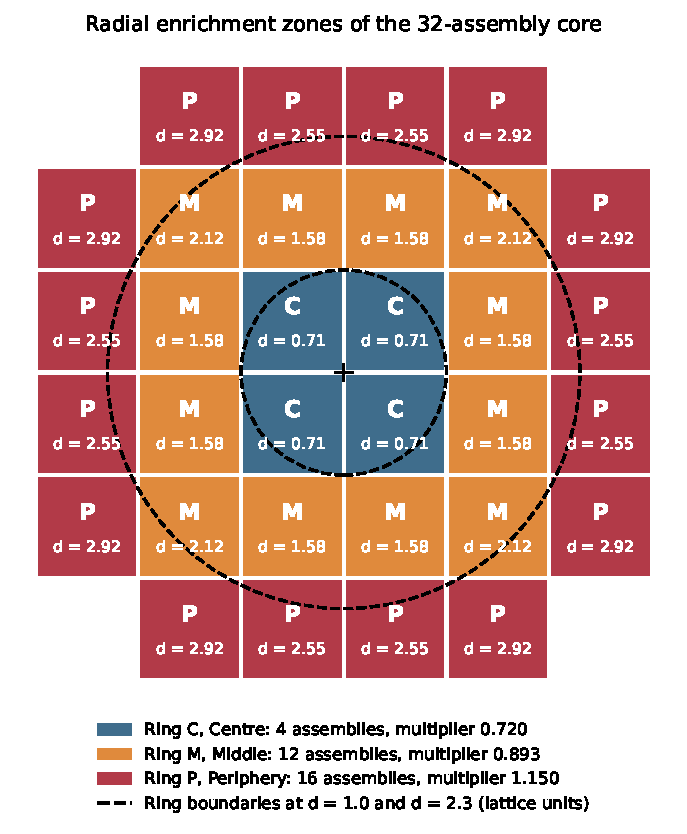
\includegraphics[width=0.75\linewidth]{images/th_zoning_rings.pdf}
  \caption{Radial enrichment rings of the 32-assembly core.}
  \label{fig:zoning-rings}
\end{figure}

The enrichment of each ring is the corresponding design enrichment
scaled by a fixed ring multiplier.

\begin{equation}
e_r \;=\; m_r \, e, \qquad r \in \{C, M, P\}
\label{eq:zoning}
\end{equation}

\noindent where the symbols have the following meaning.

\begin{itemize}
  \item $e_r$ is the as-loaded enrichment of ring $r$, in
        wt\%~$^{235}$U.

  \item $e$ is the design enrichment assigned to that ring, in
        wt\%~$^{235}$U.

  \item $m_r$ is the multiplier of ring $r$, dimensionless, equal to
        $m_C = 0.720$ for the centre, $m_M = 0.893$ for the middle
        ring and $m_P = 1.150$ for the periphery.
\end{itemize}

Only $m_C$ and $m_P$ are set. The middle multiplier is solved from the
fissile balance, which holds the assembly-weighted mean multiplier of
the core at one.

\begin{equation}
n_C\,m_C + n_M\,m_M + n_P\,m_P = n_C + n_M + n_P
\label{eq:zoning-balance}
\end{equation}

\noindent where $n_C$, $n_M$ and $n_P$ are the assembly counts of the
three rings, equal to 4, 12 and 16, dimensionless. With $m_C = 0.720$
and $m_P = 1.150$ the balance returns $m_M = 0.893$, so the zoned core
and an unzoned core built from the same enrichment variables carry the
same fissile inventory.

\subsection{How the design enrichments enter the rings}
\label{sec:meth-zoning-map}

The zoning does not assign one design enrichment to one ring. Through
Campaign 7 every assembly of the core keeps the two-zone
intra-assembly structure of Table~\ref{tab:model-geometry}, illustrated in
Figure~\ref{fig:model-geometry}(a), namely the centred $9\times9$ block
of 72 rods at $e_\mathrm{in}$ and the surrounding 192 rods at
$e_\mathrm{out}$. What the ring multiplier does is scale \emph{both}
intra-assembly enrichments of every assembly in that ring by the same
factor. From Campaign 8 the two zones collapse to the single enrichment
variable of Section~\ref{sec:meth-c8-space}, and the multiplier scales
that one value.

\begin{equation}
e_\mathrm{in}^{\,r} = m_r \, e_\mathrm{in},
\qquad
e_\mathrm{out}^{\,r} = m_r \, e_\mathrm{out}
\label{eq:zoning-pair}
\end{equation}

\noindent where the symbols have the following meaning.

\begin{itemize}
  \item $e_\mathrm{in}^{\,r}$ and $e_\mathrm{out}^{\,r}$ are the
        as-loaded inner-zone and outer-zone enrichments of an assembly
        in ring $r$, in wt\%~$^{235}$U.

  \item $e_\mathrm{in}$ and $e_\mathrm{out}$ are the two enrichment
        design variables, in wt\%~$^{235}$U.

  \item $m_r$ is the multiplier of ring $r$, dimensionless.
\end{itemize}

Three consequences follow, and all three are properties of the
implementation rather than modelling choices imposed a posteriori.

\begin{enumerate}
  \item Zoning is an enrichment redistribution only. Pitch, reflector
        thickness, gadolinia weight fraction and gadolinia rod count
        are copied to every ring unchanged, so the three ring
        assemblies are built by the same builders with the same pin
        layout as the base assembly.

  \item The gadolinia rods of each ring take their \ce{^{235}U}
        enrichment from that ring, reduced by 5 per cent, relative, per
        wt\% of \ce{Gd2O3}, with a lower limit of \SI{0.2}{wt\%}
        (Table~\ref{tab:in-materials}), following the practice for
        low-concentration gadolinia fuel~\cite{mildrum_segovia_2001}.
        The reduction lowers the fissile
        content of the urania--gadolinia rods, whose thermal conductivity
        is lower than that of \ce{UO2}~\cite{mildrum_segovia_2001}. At
        \SI{8}{wt\%} of \ce{Gd2O3}, for example, the factor is 0.60, so
        the gadolinia rods of a peripheral ring at \SI{11.5}{wt\%} carry
        \SI{6.9}{wt\%}.

  \item The zoning is applied on core solves only. The beginning-of-life
        core solve of Section~\ref{sec:meth-core-objective} and the two
        rodded solves of Section~\ref{sec:meth-ctrl} are built from the
        zoned map, while the depletion of
        Section~\ref{sec:objective_functions} runs on the assembly
        loaded at the design enrichments themselves, with no multiplier
        applied, that is $m = 1$ in
        Equation~\eqref{eq:zoning-pair}. That assembly is none of the
        three rings. It carries the core-average fissile loading, since
        the balance of Equation~\eqref{eq:zoning-balance} holds the
        assembly-weighted mean multiplier at one, and the reflective
        boundary of the depletion model replicates it into an infinite
        lattice of identical assemblies. The burnup history obtained is
        therefore the history of a core of 32 such replicas, whose
        fissile inventory equals that of the zoned core.
\end{enumerate}

%% labels of the material summarised in the zoning section, kept so that the
%% cross-references of the other chapters still resolve
\label{sec:meth-zoning-balance}

%% labels of the material reported in the results, kept so that the
%% cross-references of the other chapters still resolve
\label{sec:meth-zoning-study}\label{tab:zoning-transfer}\label{tab:zoning-grid}

\subsection{The enrichment search box}
\label{sec:meth-zoning-box}

Because the periphery carries the largest multiplier, the
low-enriched-uranium enrichment limit binds through the as-loaded peripheral ring
and not through the design variable directly. From Campaign 6 the
enrichment constraint is therefore written on the zoned map.

\begin{equation}
g_\mathrm{enr} \;=\; \max_r \left( m_r\, e \right) - 19.75 \;\le\; 0
\quad\Longrightarrow\quad
e \;\le\; \frac{19.75}{m_P} \;=\; 17.174
\label{eq:leu-box}
\end{equation}

\noindent where the symbols have the following meaning.

\begin{itemize}
  \item $g_\mathrm{enr}$ is the enrichment-limit constraint of
        Table~\ref{tab:constraints}, in wt\%~$^{235}$U, redefined on
        the zoned map from Campaign 6.

  \item $19.75$ is the low-enriched-uranium limit, in
        wt\%~$^{235}$U.

  \item $m_P$ is the peripheral multiplier, dimensionless, equal to
        1.150.

  \item $17.174$ is the resulting upper bound of both enrichment
        design variables in Campaign 6, in wt\%~$^{235}$U.
\end{itemize}

The box bound and the constraint are consistent by construction, so no
design of experiments point can violate the limit after zoning. This
removes the wasted samples observed under the earlier formulation, and
it is also what bounds $m_P$ from above.

The value of $m_P$ is the only decision of this section that is not
fixed by a measurement. A larger multiplier lowers the radial peaking
factor further, but it lowers the upper enrichment bound of
Equation~\eqref{eq:leu-box} in the same proportion, and the enrichment
limit was already active in Campaign 5. Campaign 6 therefore adopts
$m_P = 1.150$, keeping the wider enrichment range at the cost of that
peaking reduction, and a later campaign can raise $m_P$ if the
enrichment bound is no longer active. The trial on which the value was
set is reported in Section~\ref{sec:res-c5-c7}.

The zoning is the only change of Campaign 6 that acts on the
beginning-of-life power distribution, so the peaking reduction of
Campaign 6 is attributed to it (Section~\ref{sec:res-c6-compare}).
\section{Burnup limits in the simulations}
\label{sec:meth-atf}

Two assembly-average burnup limits act on the depletion of
Section~\ref{sec:bg-depletion}:

\begin{itemize}
  \item the discharge-burnup limit $B_\mathrm{burnup}$, which decides
        whether a design is acceptable and, through
        Equation~\eqref{eq:efpd}, truncates its reported cycle length,

  \item the depletion horizon $B_\mathrm{max}$, the burnup at which the
        depletion calculation is stopped.
\end{itemize}

The limit is $B_\mathrm{burnup} = \SI{55}{MWd/kgHM}$, the
assembly-average exposure limit of uranium dioxide in zirconium
cladding, set by cladding oxidation~\cite{song_sanchez_2026,alam_2019_hotchannel}.
The corresponding rod-average limit is \SI{62}{MWd/kgHM}. The limit is
applied at candidate selection to
the archived end-of-cycle burnups, so it needs no new transport
calculation. It removes designs from the fronts of Campaigns 6 and 8
and leaves those of Campaigns 7 and 9 unchanged, as reported with each
campaign.

The horizon has changed with the campaigns. Campaign 1 stopped the
depletion at \SI{35.5}{MWd/kgHM}, Campaign 2 raised it to
\SI{100}{MWd/kgHM} to test whether the censoring was an artefact of the
stopping value, and Campaigns 3 to 5 stopped at the \SI{75}{MWd/kgHM}
then adopted as the discharge limit
(Section~\ref{sec:res-c5-c7}). From Campaign 6 onwards the horizon is
$B_\mathrm{max} = \SI{100}{MWd/kgHM}$, well above the limit, so that
designs reach the end-of-cycle target before the depletion stops. Right-censoring then becomes rare, and
the objective surrogate is not trained on censored cycle lengths. Its prediction is
clipped at the horizon by Equation~\eqref{eq:efpd-clip}.

\section{Moderator temperature coefficient and the MTC boron limit}
\label{sec:meth-mtc}

The reference concentration of Section~\ref{sec:meth-boron} is held at
\SI{1000}{ppm} throughout the optimisation, so the campaigns do not test
whether a candidate can be held critical by soluble boron at an
acceptable concentration. That concentration has an upper limit. A rise
in moderator temperature lowers the moderator density, and with it the
boron number density in the core, which inserts positive reactivity.
This contribution grows with the boron concentration, and above a
certain concentration the moderator temperature coefficient becomes
positive. A positive coefficient removes the negative temperature
feedback that stabilises the core against a power excursion, and it is
not acceptable at power. The concentration at which the coefficient is
zero is therefore the upper limit of the soluble boron, called here the
MTC boron limit, and it depends on the lattice.

\subsection{Definition and evaluation}
\label{sec:meth-mtc-def}

The coefficient is evaluated as a two-point difference at constant
pressure, with the moderator density taken consistently with the
temperature from the IAPWS-IF97 formulation~\cite{wagner_iapws_if97_2000}.

\begin{equation}
\alpha_\mathrm{M}(c) = \frac{\rho\!\left(T + \Delta T,\ c\right)
- \rho\!\left(T,\ c\right)}{\Delta T}
\label{eq:mtc}
\end{equation}

\noindent where the symbols have the following meaning.

\begin{itemize}
  \item $\alpha_\mathrm{M}$ is the moderator temperature coefficient, in
        pcm per K.
  \item $\rho$ is the core reactivity at the stated moderator temperature
        and soluble boron concentration, in pcm.
  \item $T$ is the moderator temperature, in K, with the density set from
        the steam tables at the operating pressure.
  \item $\Delta T$ is the temperature perturbation, in K.
  \item $c$ is the soluble boron concentration, in ppm.
\end{itemize}

The zero-coefficient concentration $c_\mathrm{MTC}$ is the root of
Equation~\eqref{eq:mtc} in concentration. It is obtained by a weighted
straight-line fit of the coefficient against concentration over the
three scan points nearest the sign change, with the uncertainty
propagated from the fit covariance and inflated by $\sqrt{\chi^2/\nu}$
where that exceeds unity, so that it reflects a curvature of the
coefficient in boron.

\begin{equation}
\alpha_\mathrm{M}\!\left(c_\mathrm{MTC}\right) = 0
\label{eq:ceiling}
\end{equation}

\noindent where $c_\mathrm{MTC}$ is the MTC boron limit, in ppm.

A design is acceptable on this criterion when its critical concentration
at beginning of life, the root of the measured reactivity $\rho(c)$, or
its cycle maximum of Equation~\eqref{eq:c9-cmax} where a positive hump
is resolved, does not exceed $c_\mathrm{MTC}$.

The limit is evaluated outside the optimisation loop, recorded in the
archive as $g_\mathrm{boron}$ and never imposed as a constraint. Each
scan solves the zoned core at two moderator temperatures and four boron
concentrations, with two seeds per point at $100\,000$ particles and 170
batches. It was run on C8-47 at both pressures below, and on eight
Campaign 9 lattices at \SI{12.8}{MPa}, five of them also at
\SI{15.5}{MPa}.

The two best-ranked designs, C8-47 and C9-47, are scanned at each pressure both on
a two-dimensional core and on the three-dimensional core model of
Section~\ref{sec:res-c8-3d}, with the control rods fully withdrawn above the active core, so the
limit and the three-dimensional confirmation rest on the same geometry.
The pair of scans separates the axial leakage contribution to the limit
from the lattice contribution. The other seven Campaign 9 designs are
scanned on the three-dimensional core model only, because the axial
leakage contribution to the limit is measured on the two best-ranked
designs and is not the quantity that separates one design from another.

Two temperature intervals were scanned, each centred on the average
coolant temperature of a reference plant:

\begin{itemize}
  \item 570 to \SI{590}{K} at \SI{15.5}{MPa}, centred on the moderator
        temperature of \SI{580}{K} of Table~\ref{tab:model-operating},
        with moderator densities of 0.733 and \SI{0.688}{g/cm^3}
        and saturation at \SI{617.9}{K}.
        These are the primary pressure and the average coolant
        temperature of a large pressurised water
        reactor~\cite{todreas_kazimi_2012,epr_fsar_ch4},

  \item 547 to \SI{567}{K} at \SI{12.8}{MPa}, centred on \SI{557}{K},
        with moderator densities of 0.771 and \SI{0.734}{g/cm^3}
        and saturation at \SI{602.8}{K}.
        These are the system pressure, \SI{12.76}{MPa}, and the core
        average temperature, \SI{557}{K}, of the NuScale
        module~\cite{nuscale_htp2_2017}.
\end{itemize}

The limit depends on the pressure through the moderator density. No
open source gives the primary conditions of LABGENE or of any naval
propulsion reactor, so the two intervals are reference points and carry
no claim about the prototype.

The two-dimensional core omits the axial component of the moderator
feedback. When the moderator heats and expands, the axial leakage grows
and adds negative reactivity, so a limit evaluated in two dimensions
is too low. The omitted term is the difference between the three- and
the two-dimensional coefficients at the same state.

\begin{equation}
\alpha_\mathrm{ax} = \alpha_\mathrm{M}^\mathrm{3D} - \alpha_\mathrm{M}^\mathrm{2D}
\label{eq:axial-feedback}
\end{equation}

\noindent where $\alpha_\mathrm{ax}$ is the axial leakage contribution
and $\alpha_\mathrm{M}^\mathrm{3D}$ and $\alpha_\mathrm{M}^\mathrm{2D}$
are the moderator temperature coefficients in three and in two
dimensions, all in pcm per K. The two-dimensional limit is therefore
reported as a conservative bound and the three-dimensional limit as
the physical result.


%% labels of the material summarised in the definition above, kept so that the
%% cross-references of the other chapters still resolve
\label{sec:meth-mtc-checks}

%% labels of the material reported in the results, kept so that the
%% cross-references of the other chapters still resolve


\section{Transport fidelity and seeding}
\label{sec:meth-fidelity}

Every quantity returned by the evaluator is a Monte Carlo estimate,
and every one of them carries a statistical uncertainty set by the
number of neutron histories. The eigenvalue and the cycle length carry
that uncertainty alone: they are unbiased, and their error is
symmetric about the true value
(Section~\ref{sec:bg-mc-stats})~\cite{lux_koblinger_1991}. The peaking
factor $F_{\Delta H}$ carries a positive bias on top of it, for the
reason given in Section~\ref{sec:meth-fdh}. Both the bias and the
variance fall as the number of active histories grows, and the cost of
the solve grows with them.

Two settings of the transport solve therefore control the quality of
every result of this work.

\begin{itemize}
  \item \textbf{Fidelity:} the number of particles per batch and the
        number of active and inactive batches. It sets the relative
        standard error of every tally and the bias of the peaking
        estimator.

  \item \textbf{Seed policy:} the rule that assigns the initial seed of
        the pseudo-random number generator. It decides whether two
        evaluations are driven by the same random-number sequence, and
        with it whether their statistical noise is correlated.
\end{itemize}

The need to control both was established in Campaign 2
(Section~\ref{sec:res-c1c2}). At the fidelity of that campaign,
$4\,000\times60$ with one shared seed, the bias of the stored peaking
values was larger than the spread of the front they ranked, and
re-solving the candidates at high fidelity re-ordered them.

\subsection{Fidelity study}
\label{sec:meth-fid-ladder}

The fidelity of the high-fidelity search was chosen from a
seed-replicated study of the assembly estimator, in which the same
designs are repeated at $4\,000$, $16\,000$, $64\,000$ and
$256\,000$ particles with independent seeds, so that the
seed-to-seed standard deviation measures the noise and the difference
to the highest setting measures the bias. The study is reported in
Section~\ref{sec:res-c1c2}, and its outcome is the
$16\,000\times120$ setting adopted for the high-fidelity search of
Campaigns 3 and 5, which removes most of the bias for nine times the
number of active histories: \num{16000} particles over 90 active
batches is \num{1440000} histories, against \num{160000} for
\num{4000} particles over 40 active batches.

A second study measures the core estimator. The study of
Table~\ref{tab:fid-ladder} covers the assembly estimator, which is the
peaking objective of Campaigns 3 and 5 only, while from Campaign 4 the
objective is the core estimator at $100\,000\times170$ (60 inactive),
whose maximum is taken over the pins of the zoned 32-assembly core. Its
bias is taken against the extrapolation of each design to an infinite
number of histories.

\begin{equation}
F_{\Delta H}(N) = F_\infty + \frac{a}{\sqrt{N}}
\label{eq:fdh-extrap}
\end{equation}

\noindent where $F_{\Delta H}(N)$ is the mean over the seeds of the core
peaking factor at $N$ active histories, the particles per batch
multiplied by the 110 active batches, $F_\infty$ is the extrapolated
value and $a$ the fitted bias coefficient, all dimensionless. The
extrapolation assumes that the bias falls as $1/\sqrt{N}$. The study
that applies it is reported in Section~\ref{sec:res-c9-peaking}.

\subsection{Transport settings per campaign}
\label{sec:meth-fid-settings}

Table~\ref{tab:fidelity} lists the transport settings of every campaign
and evaluation stage. A campaign row gives the settings of the assembly
depletion run in every evaluation of that campaign. The other rows are
evaluation stages, that is, transport calculations run in addition to
the assembly depletion: the core solves inside each evaluation from
Campaign 4, and the two stages at higher fidelity with which the
finalists of Campaigns 2 and 3 were ranked.
The settings are stored in each campaign checkpoint and cannot change
during a campaign.

\begin{table}[htbp]
  \centering
  \begin{threeparttable}
  \caption{Transport settings per campaign and per evaluation stage.}
  \label{tab:fidelity}
  \small
  \begin{tabularx}{\textwidth}{@{}>{\raggedright\arraybackslash}p{0.21\textwidth}c>{\raggedright\arraybackslash}p{0.17\textwidth}>{\raggedright\arraybackslash}X@{}}
    \toprule
    Stage & Particles $\times$ batches\tnote{a} & Seed policy & Role \\
    \midrule
    Campaign 1     & $4\,000\times60$ (20)    & shared              & verification \\
    Campaign 2     & $4\,000\times60$ (20)    & shared              & low-fidelity search \\
    Campaign 3     & $16\,000\times120$ (30)  & per-design          & high-fidelity search \\
    C4 core solve  & $100\,000\times170$ (60) & per-design, salted  & core solve: $F_{\Delta H}$ \\
    Campaign 5     & $16\,000\times120$ (30)  & per-design          & high-fidelity search \\
    C5 confirmation & $200\,000\times260$ (80) & replicated, 8 seeds & confirmation of one design \\
    Campaign 6     & $4\,000\times60$ (20)    & per-design          & low-fidelity search \\
    C6 core solve  & $100\,000\times170$ (60) & per-design, salted  & core solve: $F_{\Delta H}$, $k$ window \\
    Campaign 7     & $4\,000\times60$ (20)    & per-design          & low-fidelity search \\
    C7 core solves & $100\,000\times170$ (60) & per-design, salted  & core solves: $F_{\Delta H}$, $k$ window, one rodded solve \\
    Campaign 8     & $4\,000\times60$ (20)    & per-design          & low-fidelity search \\
    C8 core solves & $100\,000\times170$ (60) & per-design, salted  & core solves: $F_{\Delta H}$, $k$ window, two rodded solves \\
    Campaign 9     & $4\,000\times60$ (20)    & per-design          & low-fidelity search \\
    C9 core solves & $100\,000\times170$ (60) & per-design, salted  & core solves: as C8, and unrodded at 2000 and 3000\,ppm for $c_\mathrm{max}$ \\
    Preselection   & $64\,000\times120$ (30)  & replicated          & selection, first stage \\
    Confirmation   & $256\,000\times120$ (30) & replicated, 8 seeds & selection, second stage \\
    \bottomrule
  \end{tabularx}
  \begin{tablenotes}[flushleft]\footnotesize
    \item[a] Inactive batches in parentheses.
  \end{tablenotes}
  \end{threeparttable}
\end{table}

From Campaign 6 the assembly depletion returns to $4\,000\times60$,
the setting of Campaigns 1 and 2, after the $16\,000\times120$ of
Campaigns 3 and 5. The change is part of a two-tier fidelity strategy. The search runs at low fidelity,
where it needs many evaluations and the cycle length can carry a known
bias, while the core solves inside each evaluation, which evaluate
$F_{\Delta H}$, the reactivity window and the controllability constraints, stay at
$100\,000\times170$. Feasibility and peaking are therefore computed at
full fidelity, and only the cycle length carries the low-fidelity bias,
so the cycle lengths of Campaigns 6 to 9 are not comparable with those
of Campaigns 3 to 5 without a measured inter-fidelity shift, which
Section~\ref{sec:res-c9-dep-check} reports. The fidelity is held
constant across all blocks of a campaign, because a surrogate trained
on a mixed-fidelity archive carries a bias that changes with the
evaluation date and cannot be corrected a posteriori. The second tier
is the three-dimensional confirmation of the Campaign 8 candidates of
Section~\ref{sec:res-c8-limits}, and every Campaign 6 and Campaign 7
cycle length remains a low-fidelity value.

\subsection{Seed policy}
\label{sec:meth-fid-seed}

OpenMC initialises its pseudo-random number generator with the same
default seed in every run unless another seed is set. With that
default, every design is computed on the same random-number sequence.
Two similar problems driven by one sequence consume the same random
numbers at the same points of each history, so the source sites and
the interaction outcomes they sample coincide until the two models
differ. Their tally errors then share a common component and the noise
of different designs is positively correlated, which is the mechanism
of correlated sampling~\cite{lux_koblinger_1991}.

The coupling is partial
here, because two designs differ in geometry and composition and their
histories diverge as soon as that difference changes a sampled
interaction. Campaigns 1 and 2 ran on that default seed, so every
design of both campaigns shared one sequence. The effect was detected
in Campaign 2, where re-solving the finalists at high fidelity with
independent seeds did not preserve their ranking
(Section~\ref{sec:res-c1c2}).

From Campaign 3 each design receives its own seed, a CRC32 hash of its
design vector. Each core solve adds a fixed string to the hash, the
salt, so that the assembly and core solves of one design also run on
different sequences. The policy has two properties.

\begin{itemize}
  \item \textbf{Reproducibility:} the seed depends only on the design,
        so repeating an evaluation returns the same result.

  \item \textbf{Independent noise:} the noise of two designs is
        uncorrelated, which is the independent and identically
        distributed noise assumed by the white-noise term of the
        Gaussian-process kernel of Section~\ref{sec:bg-gp}.
\end{itemize}

%% labels of the removed section, kept so that the cross-references still resolve
\label{sec:meth-stats}\label{eq:noise-margin-set}

\section{Surrogate-assisted active-learning loop}
\label{sec:meth-loop}

The loop is described in Section~\ref{sec:bg-al} and
Figure~\ref{fig:bg-al}. One iteration has four steps.

\begin{enumerate}
  \item A Latin-hypercube design of experiments.

  \item Gaussian-process surrogates of the objectives and the
        constraints (Section~\ref{sec:bg-gp}).

  \item An NSGA-II search on the surrogates
        (Section~\ref{sec:bg-nsga2}).

  \item An infill batch evaluated with OpenMC.
\end{enumerate}

This section fixes what Chapter~\ref{ch:background} leaves open.

\begin{enumerate}
  \item The stopping rule.

  \item The settings with which the loop was run.

  \item The acquisition function, with the three revisions that
        Campaign 6 made necessary.
\end{enumerate}

Figure~\ref{fig:meth-loop-flow} summarises one iteration as
implemented.

\begin{figure}[htbp]
  \centering
  \resizebox{\textwidth}{!}{%
  \begin{tikzpicture}[
      box/.style={draw, rounded corners=2pt, align=center, font=\small,
                  text width=2.35cm, minimum height=1.35cm, fill=blue!6},
      outbox/.style={box, fill=green!10},
      arr/.style={-{Stealth[length=2.2mm]}, thick},
      node distance=0.45cm]
    \node[box] (a) {Archive of OpenMC evaluations};
    \node[box, right=of a] (b) {Fit one GP per objective and constraint};
    \node[box, right=of b] (c) {NSGA-II on the surrogates, $300\times400$};
    \node[box, right=of c] (d) {Rank-1 candidate set};
    \node[box, right=of d] (e) {Acquisition: infill batch of six};
    \node[box, right=of e] (f) {OpenMC evaluation and checkpoint};
    \node[outbox, right=0.9cm of f] (g) {Pareto front of the archive};
    \draw[arr] (a) -- (b);
    \draw[arr] (b) -- (c);
    \draw[arr] (c) -- (d);
    \draw[arr] (d) -- (e);
    \draw[arr] (e) -- (f);
    \draw[arr] (f) -- node[above, font=\footnotesize, align=center] {rule\\met} (g);
    \draw[arr] (f.south) -- ++(0,-0.55) -| node[pos=0.25, below, font=\footnotesize]
      {Stopping rule not met: next iteration} (a.south);
  \end{tikzpicture}}
  \caption{One iteration of the surrogate-assisted loop.}
  \label{fig:meth-loop-flow}
\end{figure}

\subsection{Stopping rule}
\label{sec:meth-loop-stop}

The loop stops when two conditions hold together. The first uses the
relative gain of the hypervolume of Section~\ref{sec:bg-hv} in each
iteration.

\begin{equation}
\Delta_t = \frac{H_t - H_{t-1}}{H_{t-1}}
\label{eq:hv-stop}
\end{equation}

\noindent where $\Delta_t$ is the relative gain of iteration $t$,
dimensionless, and $H_t$ and $H_{t-1}$ are the hypervolumes of the
archive after iterations $t$ and $t-1$, Equation~\eqref{eq:hv}, against
the fixed reference point. The condition is that the gain stays below
one per cent in each of the last three iterations:

\begin{equation}
\Delta_{T-2} < 0.01, \qquad \Delta_{T-1} < 0.01, \qquad \Delta_{T} < 0.01
\label{eq:hv-stop-cond}
\end{equation}

\noindent where $T$ is the last iteration completed.

The second condition is that no censored design remains on the Pareto
front, so that the front is fully resolved. A three-iteration window is
used because the gains are not monotonic.

The rule is necessary and not sufficient, since it can fire while the
acquisition selects near-duplicate or infeasible designs
(Section~\ref{sec:res-c6-margin}). Two health indicators are therefore recorded at every iteration and
checked before the rule is accepted:

\begin{itemize}
  \item the number of candidates that pass the feasibility margin of
        Equation~\eqref{eq:feas-margin}, which shows whether the
        constraint surrogate is still changing,

  \item the depth of the separation relaxation of
        Section~\ref{sec:meth-acq}, which shows whether the surrogate
        front still contains new designs.
\end{itemize}

Campaigns 3 and 6 met the rule. Campaigns 8 and 9 were stopped at
their budget of 60 evaluations, one iteration short of the window, and
their fronts are reported as the best available at that budget
(Sections~\ref{sec:res-c8-limits} and~\ref{sec:res-c9-convergence}).

\subsection{Surrogate and loop settings}
\label{sec:meth-loop-settings}

The inputs and outputs of every Gaussian process are standardised, so
that one dimensionless length-scale per variable of
Equation~\eqref{eq:kernel-r} is meaningful.

\begin{equation}
z_d = \frac{x_d - \bar{x}_d}{s_d}
\label{eq:standardise}
\end{equation}

\noindent where $z_d$ is the standardised value of variable $d$,
dimensionless, and $\bar{x}_d$ and $s_d$ are the mean and the standard
deviation of that variable over the archive, in its native unit. The
outputs are standardised in the same way.

One independent Gaussian process with the kernel of
Equation~\eqref{eq:kernel} is fitted to each output, the two objectives
and every constraint that is not computed analytically. Its
hyperparameters are refitted on the whole archive by maximising the log
marginal likelihood~\cite{rasmussen_gp_2006}. The refit is performed
once per iteration of the active-learning loop, that is once the
OpenMC evaluations of an infill batch have entered the archive. The
generations of the NSGA-II search run on surrogates whose
hyperparameters are held fixed and are not refitted.

\begin{equation}
\log p(\mathbf{y} \mid \boldsymbol{\theta})
= -\tfrac{1}{2}\,\mathbf{y}^{\mathsf T}
\left( \mathbf{K} + \sigma_n^{2}\mathbf{I} \right)^{-1} \mathbf{y}
- \tfrac{1}{2} \log \left| \mathbf{K} + \sigma_n^{2}\mathbf{I} \right|
- \tfrac{n}{2} \log 2\pi
\label{eq:gp-lml}
\end{equation}

\noindent where $\boldsymbol{\theta} = (\ell_1, \dots, \ell_D,
\sigma_f, \sigma_n)$ is the vector of hyperparameters and the other
symbols are those of Equations~\eqref{eq:kernel} to~\eqref{eq:gp-var}.
The maximisation is restarted from four random starting points to avoid
a local maximum. The first term rewards the fit to the archive and the
second penalises model complexity, so the fitted length-scales do not
simply interpolate the noise.

Table~\ref{tab:loop-settings} gives the loop settings of Campaigns 3
to 9. Campaign 3 is the first campaign in which per-design seeding made
the archive statistically consistent.

\begin{table}[htbp]
  \centering
  \small
  \caption{Loop settings per campaign.}
  \label{tab:loop-settings}
  \begin{tabular}{@{}lccccl@{}}
    \toprule
    Campaign & Initial designs & Batch & Iterations & Total & End \\
    \midrule
    C3 & 36 & 6 & 6  & 72  & stopping rule met \\
    C4 & 36 & 6 & 3  & 54  & -- \\
    C5 & 42 & 6 & 3  & 60  & -- \\
    C6 & 42 & 6 & 12 & 114 & stopping rule met \\
    C7 & 42 & 6 & 3  & 60  & -- \\
    C8 & 36 & 6 & 4  & 60  & budget, best available \\
    C9 & 24 & 6 & 6  & 60  & budget, best available \\
    \bottomrule
  \end{tabular}
\end{table}

\subsection{Acquisition function}
\label{sec:meth-acq}

The infill batch is selected from the rank-1 set of the final NSGA-II
population on the surrogates. The base criterion, whose steps are
listed in Section~\ref{sec:bg-al}, ranks the candidates by their
aggregated predictive uncertainty.

\begin{equation}
a_i \;=\; \sum_{m=1}^{2} \frac{\sigma_{im}}{\max_{l}\,\sigma_{lm}}
\label{eq:acq-score}
\end{equation}

\noindent where $a_i$ is the acquisition score of candidate $i$,
dimensionless, and $\sigma_{im}$ is the posterior standard deviation of
objective $m$ at candidate $i$ from Equation~\eqref{eq:gp-var}. The
index $l$ runs over the same rank-1 candidate set as $i$, so
$\max_l \sigma_{lm}$ is the largest posterior standard deviation of
objective $m$ over that set and each term of the sum lies between zero
and one. The normalisation is per objective, since the two are measured
in different units and the larger of them would otherwise set the
ranking on its own. This is a pure exploration criterion in the sense
of~\cite{forrester_book_2008}.

Campaign 6 exposed three failures of the base criterion, and each was
corrected by one revision, introduced one per block so that each effect
is attributable (Section~\ref{sec:res-c6-defects}).
Figure~\ref{fig:meth-acq-flow} shows the resulting selection.

\begin{itemize}
  \item \textbf{Horizon-aware surrogate objective:} the problem is
        extrapolation beyond the depletion horizon. The OpenMC
        evaluator stops every depletion at $B_\mathrm{max}$, so a
        design that has not reached the target is recorded with the
        cycle length it had at the horizon. That value is a lower bound
        on the cycle length the design would have reached, since its
        depletion was stopped before the target. A Gaussian process
        trained on the archive nonetheless predicts values above the
        horizon, and the search then concentrates on predictions that
        the evaluator cannot return. The surrogate objective is clipped at the horizon
        before it enters the search.

        \begin{equation}
        \tilde{f}_1(\mathbf{x}) \;=\;
        \max\!\left( f_1(\mathbf{x}),\; -E_\mathrm{max} \right),
        \qquad
        E_\mathrm{max} \;=\; \frac{1000\, B_\mathrm{max}}{P_\mathrm{spec}}
        \label{eq:efpd-clip}
        \end{equation}

        Here $\tilde{f}_1$ and $f_1$ are the clipped and the raw
        predictions of the first objective in minimisation form, the
        negative cycle length in days, and $E_\mathrm{max}$ is the
        horizon expressed as a cycle length, \num{10016.7} days at
        $B_\mathrm{max} = \SI{100}{MWd/kgHM}$ with the specific power
        $P_\mathrm{spec}$ of Table~\ref{tab:model-operating}. On the
        clipped plateau non-dominated sorting ranks the designs by
        peaking alone, which is how the constrained-domination principle
        ranks censored designs~\cite{deb_nsga2_2002}.

  \item \textbf{Feasibility margin:} the base criterion of
        Equation~\eqref{eq:acq-score} is defined on the objective
        surrogates alone, so the constraint surrogates never enter the
        ranking. At distances from the archive designs larger than
        the kernel length-scales $\ell_d$, the posterior mean of
        Equation~\eqref{eq:gp-mean} reverts to the prior mean, the
        average of the archive, so it predicts a constraint value
        typical of the evaluated designs even in regions that violate
        the constraint (Section~\ref{sec:res-c6-defects}). Every
        candidate is therefore scored on the
        constraint surrogates with an uncertainty margin.

        \begin{equation}
        s_i \;=\; \max_{j \,\in\, \mathcal{G}_\mathrm{GP}}
        \left( \mu_{ij} + \kappa\,\sigma_{ij} \right)
        \label{eq:feas-margin}
        \end{equation}

        \noindent where $s_i$ is the margin score of candidate $i$ in the
        normalised constraint units of Equation~\eqref{eq:cv-norm},
        $\mathcal{G}_\mathrm{GP}$ is the set of constraints predicted by
        a surrogate, $\mu_{ij}$ and $\sigma_{ij}$ are the posterior mean
        and standard deviation of constraint $j$, and
        $\kappa = 1.5$ from Campaign 6. Candidates with $s_i \le 0$ are
        ranked first by $a_i$, and the others follow by ascending $s_i$,
        so the batch is always filled with the least risky designs. The
        construction is the deterministic counterpart of the
        probability-of-feasibility weighting~\cite{forrester_book_2008}
        and applies the rule of safe Bayesian optimisation, in which a
        point is admitted only where the confidence bound of every
        constraint is satisfied~\cite{sui_safeopt_2015}. Its effect
        on Campaign 6 is reported in Section~\ref{sec:res-c5-c7}.

  \item \textbf{Batch diversity:} the problem is batch collapse. The
        posterior standard deviation is a continuous function of the
        design, so the candidates with the largest $a_i$ are clustered
        in the neighbourhood of the same local maximum of
        Equation~\eqref{eq:gp-var}. The batch is therefore built by sequential
        selection down the ranking under a minimum-distance constraint.
        A candidate is accepted only if its normalised distance to
        every archive design and to every design already in the batch
        is at least $\delta_\mathrm{min}$.

        \begin{equation}
        d(\mathbf{a},\mathbf{b}) \;=\;
        \frac{1}{\sqrt{n_x}}
        \left\lVert \frac{\mathbf{a}-\mathbf{b}}
        {\mathbf{x}_u-\mathbf{x}_l} \right\rVert_2
        \;\ge\; \delta_\mathrm{min}
        \label{eq:batch-div}
        \end{equation}

        \noindent where $\mathbf{a}$ and $\mathbf{b}$ are two design
        vectors, $\mathbf{x}_l$ and $\mathbf{x}_u$ are the bounds of
        the design space, so that each variable is divided by its own
        range, and $n_x$ is the number of design variables, so that $\delta_\mathrm{min}$
        reads as a mean fraction of range per variable. The threshold
        is a lower bound on the separation, so a larger
        $\delta_\mathrm{min}$ forces the picks further apart and a
        smaller one admits picks that are closer together.

        If the rank-1 set cannot fill the batch at the configured
        value, $\delta_\mathrm{min}$ is halved and the selection is
        repeated, and only when the candidates are exhausted is the
        batch completed with random space-filling designs. That
        halving guarantees that the batch is filled, at the cost of
        the diversity it was imposed to protect. The configured value
        therefore matters. From 0.14 the first relaxation still demands
        0.07, above the 0.05 at which Campaign 7 began.

        A campaign may run straight through to the stopping rule, but
        it may equally be stopped between infill blocks and relaunched,
        so $\delta_\mathrm{min}$ can be changed before the next batch
        and an observed collapse answered by forcing the following
        batch further apart. That possibility has existed since the
        block of Campaign 6 that introduced the revision, and
        Campaign 6 ran at $\delta_\mathrm{min} = 0.14$.

        At that time 0.14 was not the default of the code, which
        stood at 0.05, so the value had to be passed explicitly at
        launch. Campaign 7 was launched without it and ran its three
        blocks at 0.05, two of which collapsed, and that was identified
        only once the campaign had finished
        (Section~\ref{sec:res-c7-blocks}). Campaigns 8 and 9 both ran
        at $\delta_\mathrm{min} = 0.14$, passed explicitly to the
        launcher, and 0.14 is now the default of the code, so a launch
        that omits the argument reproduces the adopted policy. The
        value of every campaign is recorded in its checkpoint.

        The collapse is possible at a nominally satisfied
        $\delta_\mathrm{min}$ because the distance is a mean over all
        variables, so two variables can account for it while the others
        take repeated values.
\end{itemize}

The margin discriminates only while the candidates are located strictly
inside the feasible region. When a constraint is active at the optimum,
the search places its candidates on the predicted boundary of that
constraint, where $\mu_{ij} \approx 0$, and no candidate can satisfy a
positive margin. Every batch then comes from the fallback ordering, and
the count of margin-feasible candidates is zero whether or not the
constraint surrogate is still learning. Campaign 9 is in this
situation, and Section~\ref{sec:res-c9-convergence} reports the
consequences.

\begin{figure}[htbp]
  \centering
  \resizebox{\textwidth}{!}{%
  \begin{tikzpicture}[
      box/.style={draw, rounded corners=2pt, align=center, font=\small,
                  text width=2.45cm, minimum height=1.45cm, fill=blue!6},
      outbox/.style={box, fill=green!10},
      arr/.style={-{Stealth[length=2.2mm]}, thick},
      node distance=0.45cm]
    \node[box] (a) {Surrogate objective clipped at the horizon, Eq.~\eqref{eq:efpd-clip}};
    \node[box, right=of a] (b) {NSGA-II rank-1 candidates};
    \node[box, right=of b] (c) {Margin score $s_i$, Eq.~\eqref{eq:feas-margin}};
    \node[box, right=of c] (d) {Order: $s_i \le 0$ by $a_i$, then ascending $s_i$};
    \node[box, right=of d] (e) {Sequential selection with $d \ge \delta_\mathrm{min}$, Eq.~\eqref{eq:batch-div}};
    \node[outbox, right=of e] (f) {Infill batch of six designs};
    \draw[arr] (a) -- (b);
    \draw[arr] (b) -- (c);
    \draw[arr] (c) -- (d);
    \draw[arr] (d) -- (e);
    \draw[arr] (e) -- (f);
    \draw[arr] (e.south) -- ++(0,-0.5) -| node[pos=0.25, below, font=\footnotesize]
      {batch not full: halve $\delta_\mathrm{min}$} (d.south);
  \end{tikzpicture}}
  \caption{Selection of the infill batch from the surrogate search.}
  \label{fig:meth-acq-flow}
\end{figure}

\subsection{Search setting on the surrogate}
\label{sec:meth-nsga-setting}

The population size and the number of generations of the NSGA-II
search on the surrogates, $300\times400$, were fixed by a sensitivity
study on fixed surrogates
(Section~\ref{sec:res-c5-c7}) and are used from Campaign 6 onward,
since one search costs seconds against minutes for one transport
evaluation and the largest setting tested therefore carries no
computational penalty.


% ---------------------------------------------------------------------
%  Validation of the optimisation framework.
%  Protocol of the two validation exercises run on Campaign 8:
%    Step 0, cross-validation of the surrogate on the archive and
%            stability of the archived front, at no transport cost.
%    Step 3, verification of the surrogate-assisted search against
%            exhaustive enumeration on a two-variable slice.
%  The numerical results are in Sections \ref{sec:res-c8-cv},
%  \ref{sec:res-c8-stability} and \ref{sec:res-c8-valgrid}.
%  Scripts: c8_surrogate_cv.py, c8_front_stability.py, valgrid_compare.py.
% ---------------------------------------------------------------------

\section{Proxy validation and the core-level objective (Campaign 4)}
\label{sec:meth-core-objective}

Campaigns 1 to 3 minimised the radial peaking factor of the reflective
assembly (Section~\ref{sec:meth-fdh}), a proxy of the core value that
contains no radial power gradient between assemblies and can rank designs
differently from the core (Section~\ref{sec:res-corevalidation}). The
proxy was tested against the core value with three instruments, and
Campaign 4 replaced it with a direct core calculation.

\begin{itemize}
  \item \textbf{Finalist validation:} each Pareto finalist is solved as
        the full core at beginning of life with a pin-wise fission-power
        tally and replicated seeds. The ratio
        $F_{\Delta H}^\mathrm{core}/F_{\Delta H}^\mathrm{asm}$ is the
        model discrepancy, and the same solve checks the
        leakage-corrected
        target of Section~\ref{sec:meth-ktarget}.

  \item \textbf{Archive rescoring:} every feasible design is recomputed
        at core level, with three seeds and then eight near the minimum,
        and the Spearman rank correlation between proxy and core values
        measures whether the proxy discarded better designs.

  \item \textbf{Discrepancy model:} the multiplicative discrepancy
        between the two levels is fitted following Kennedy and
        O'Hagan~\cite{kennedy_ohagan_2000,forrester_book_2008}.
\end{itemize}

\begin{equation}
\frac{F_{\Delta H}^\mathrm{core}}{F_{\Delta H}^\mathrm{asm}}
\approx a + b\,t_\mathrm{refl} + c\,p
\label{eq:bridge}
\end{equation}

\noindent where the symbols have the following meaning.

\begin{itemize}
  \item $F_{\Delta H}^\mathrm{core}$ and $F_{\Delta H}^\mathrm{asm}$
        are the peaking factors of the same design at core and assembly
        level, dimensionless.

  \item $a$ is the fitted intercept, dimensionless.

  \item $b$ is the fitted coefficient of the reflector thickness, in
        cm$^{-1}$.

  \item $c$ is the fitted coefficient of the pin pitch, in cm$^{-1}$.

  \item $t_\mathrm{refl}$ is the reflector thickness, in cm.

  \item $p$ is the pin pitch, in cm.
\end{itemize}

The fitted values on the Campaign 3 archive are given in
Equation~\eqref{eq:bridge-fit}.

The Campaign 4 decision is justified by the computational cost of the
change. The core BOL solve takes about \SI{104}{s} against an
evaluation of about \SI{110}{min}.

\begin{equation}
\frac{\Delta t}{t} \approx \frac{113 - 110}{110} \approx 3\%
\label{eq:corecost}
\end{equation}

\noindent where $\Delta t$ is the wall-time increment of one evaluation
when the core solve is added and $t$ the wall time without it, with 113
and \SI{110}{min} the measured wall times with and without the core
solve.

At this cost the core peaking factor is computed directly in every
evaluation, instead of being estimated from the assembly value through
the discrepancy model of Equation~\eqref{eq:bridge}. $F_{\Delta H}$ and
$g_\mathrm{peak}$ are evaluated on the core solve, and the assembly
value is stored as a diagnostic quantity. The cycle length is still
obtained from the assembly depletion with the leakage-corrected target,
because a full-core depletion in every evaluation is not affordable.
The proxy is therefore kept only where the direct calculation is too
expensive.

Both peaking factors are archived on every evaluation from Campaign~4
onward, the core value under the objective and the assembly value as a
diagnostic, so the ratio of Equation~\eqref{eq:bridge} can be
recomputed on any later archive without further transport.
Section~\ref{sec:res-proxy-gap-zoned} recomputes it on the zoned
archives of Campaigns~6 to~8.


\section{Validation of the optimisation framework}
\label{sec:validation-framework}

Three questions are answered before the fronts of Campaigns 8 and 9 are
interpreted, one in each of the subsections that follow.

\begin{enumerate}
  \item Whether the surrogate on which the acquisition was computed
        predicts the transport results accurately enough, with
        calibrated uncertainties
        (Section~\ref{sec:validation-surrogate}).

  \item Whether the front is a converged set rather than an artefact of
        the evaluation at which the campaign stopped or of the Monte
        Carlo noise of the transport solves
        (Section~\ref{sec:validation-front}).

  \item Whether the surrogate-assisted search recovers the Pareto front
        that an exhaustive enumeration finds, and at what fraction of
        the enumeration cost (Section~\ref{sec:validation-grid}).
\end{enumerate}

The first two are answered on the archive, the database of every design
evaluated by the transport code with its objectives and constraints, at
no additional transport cost, and they are answered for both campaigns.
The third requires new transport solves and is therefore restricted to
a two-dimensional subspace of the design space, in which the other
variables are held constant and exhaustive enumeration is affordable.

\subsection{Cross-validation of the surrogate on the archive}
\label{sec:validation-surrogate}

The surrogate under test is the one of the loop of
Section~\ref{sec:meth-loop}, with the kernel of
Equation~\eqref{eq:kernel}, the standardisation of
Equation~\eqref{eq:standardise} and the normalised constraints of
Equation~\eqref{eq:cv-norm}, fitted on all archived designs, feasible
and infeasible.

Two protocols are applied. Cross-validation of a surrogate against the
data it was fitted on is standard practice in engineering
design~\cite{forrester_book_2008}, and the second protocol carries that
idea into the sequential setting of the loop, where the surrogate that
decided an infill batch is the one fitted before that batch was
evaluated. Figure~\ref{fig:val-protocols} summarises them.

\begin{itemize}
  \item \textbf{Leave-one-out cross-validation (LOOCV):} each of the $N$
        archived designs is held out once, the surrogate is refitted on
        the remaining $N-1$ designs, and the held-out design is
        predicted. It is the leave-one-out predictive check of a
        Gaussian process~\cite{rasmussen_gp_2006}, and it measures the
        predictive accuracy of the surrogate trained on the final
        archive.

  \item \textbf{Walk-forward validation:} for each infill block, the
        surrogate is trained only on the evaluations completed before
        that block and predicts the designs of the block. It measures
        the predictive accuracy at the time of the acquisition
        decision, on the designs that the acquisition selected.
\end{itemize}

\begin{figure}[htbp]
  \centering
  \resizebox{\textwidth}{!}{%
  \begin{tikzpicture}[
      box/.style={draw, rounded corners=2pt, align=center, font=\small,
                  text width=2.6cm, minimum height=1.25cm, fill=blue!6},
      lab/.style={font=\small\bfseries, align=right, text width=2.3cm},
      arr/.style={-{Stealth[length=2.2mm]}, thick},
      node distance=0.45cm]
    \node[lab] (l1) {Leave-one-out};
    \node[box, right=of l1] (a1) {Archive of $N$ designs};
    \node[box, right=of a1] (b1) {Remove design $i$};
    \node[box, right=of b1] (c1) {Refit the GPs on $N-1$ designs};
    \node[box, right=of c1] (d1) {Predict design $i$};
    \node[box, right=of d1] (e1) {Compare with the transport value};
    \draw[arr] (a1) -- (b1);
    \draw[arr] (b1) -- (c1);
    \draw[arr] (c1) -- (d1);
    \draw[arr] (d1) -- (e1);
    \draw[arr] (e1.south) -- ++(0,-0.35) -| node[pos=0.25, below, font=\footnotesize]
      {next $i$, until $i = N$} (b1.south);
    \node[lab, below=1.5cm of l1] (l2) {Walk-forward};
    \node[box, right=of l2] (a2) {Evaluations before block $b$};
    \node[box, right=of a2] (b2) {Fit the GPs};
    \node[box, right=of b2] (c2) {Predict the designs of block $b$};
    \node[box, right=of c2] (d2) {Compare with the transport values};
    \node[box, right=of d2] (e2) {Add block $b$ to the training set};
    \draw[arr] (a2) -- (b2);
    \draw[arr] (b2) -- (c2);
    \draw[arr] (c2) -- (d2);
    \draw[arr] (d2) -- (e2);
    \draw[arr] (e2.south) -- ++(0,-0.35) -| node[pos=0.25, below, font=\footnotesize]
      {next block $b+1$} (a2.south);
  \end{tikzpicture}}
  \caption{Leave-one-out and walk-forward validation of the surrogate.}
  \label{fig:val-protocols}
\end{figure}

For each output, the held-out predictions give the root mean square
error (RMSE) of the predictive mean against the transport value, the
coefficient of determination $R^2$, and the calibration of the
predictive uncertainty.

\begin{equation}
  s_z = \sqrt{\frac{1}{N}\sum_{i=1}^{N}\left(z_i - \bar{z}\right)^2},
  \qquad z_i = \frac{y_i - \mu_i}{\sigma_i}
  \label{eq:val-sz}
\end{equation}

\noindent where $y_i$ is the transport value of design $i$, $\mu_i$ and
$\sigma_i$ the predictive mean and standard deviation, $\bar{z}$ the
mean of the $N$ standardised residuals $z_i$, and $s_z$ their standard
deviation, dimensionless, equal to 1 for a calibrated predictor, above 1
for an over-confident one and below 1 for an under-confident one.

The coverage of the one-sigma and two-sigma predictive intervals, with
nominal values 0.683 and 0.954 for Gaussian errors, and the Spearman
rank correlation between predicted and true values complete the set.
The rank correlation is included because the acquisition ranks
candidates rather than reading their absolute values. Constraint columns are converted back to
the eigenvalues they encode, so that errors can be read in reactivity
units.

The feasibility verdict of the surrogate is also scored. Two rules are
compared against the true verdict of the transport solves. The mean rule
declares a design feasible when every predicted constraint mean is at or
below zero. The margin rule, used by the acquisition, requires every
predicted constraint mean plus $\kappa$ predictive standard deviations to
be at or below zero, with $\kappa$ the campaign value of
Section~\ref{sec:meth-acq}.

The results are reported in Section~\ref{sec:res-c8-cv} for Campaign 8
and in Section~\ref{sec:res-c9-convergence} for Campaign 9.

\subsection{Stability of the archived front}
\label{sec:validation-front}

The front is the result the campaign delivers, so it has to be shown
that it is a converged set and not an artefact of the evaluation at
which the campaign stopped or of the Monte Carlo noise of the transport
solves. Two tests are applied, one against each of those two
possibilities. The first uses the hypervolume of the non-dominated set
as its convergence measure~\cite{coello_2007}, and the second is the
treatment of an objective that carries a Monte Carlo uncertainty,
applied to an optimisation driven by such
solves~\cite{erdem_2025_mc_uncertainty}.

The first test follows the front through the campaign. The feasible
non-dominated set is recomputed after every evaluation, in the order of
execution, together with its hypervolume at the fixed reference point,
defined once from the design of experiments of the campaign. For each
member of the final front, the evaluation at which it joined the set is
recorded, and so is every design that a later evaluation dominated and
removed from the set. A front whose members all joined in the first
blocks and were never removed is converged. A front that gains a member
in its last block is not, and its composition depends on where the
campaign stopped.

This is a different question from the stopping rule of
Section~\ref{sec:meth-loop-stop}. That rule is a decision taken during
the campaign on one scalar, the relative gain of the hypervolume, and
it fires when that gain stays below one per cent for three iterations.
A design can join the front at the last evaluation while contributing
almost nothing to the hypervolume, so the rule can be met on a front
whose membership is still changing. The test reads the membership
itself, after the campaign, and Campaign 8 is the case that separates
the two.

The second test perturbs the front. The objectives of every feasible
design are perturbed by Gaussian noise representing the Monte Carlo
uncertainty of the transport solves, the non-dominated set is
recomputed, and the probability that each design belongs to it is
estimated over many replicates. The cycle length noise of a design
follows from the eigenvalue uncertainty through the mean reactivity
slope of that design.

\begin{equation}
  \sigma_{\mathrm{cycle}} = \sqrt{2}\,\frac{\sigma_k}{\left(k_{\mathrm{BOL}} - k_{\mathrm{target}}\right)/T}
  \label{eq:val-sigma-cycle}
\end{equation}

\noindent where $\sigma_\mathrm{cycle}$ is the one-sigma noise on the
cycle length in EFPD, $\sigma_k$ the one-sigma uncertainty of one
depletion eigenvalue, $k_\mathrm{BOL}$ the beginning-of-life
multiplication factor of the assembly, $k_\mathrm{target}$ the
end-of-cycle target of Section~\ref{sec:meth-ktarget} and $T$ the
archived cycle length in EFPD. The factor $\sqrt{2}$ accounts for the
interpolation of the end-of-cycle crossing between two independently
noisy eigenvalues.

Two front members whose membership probabilities are well below one are
not resolved by the transport statistics and are reported as
equivalent. The results of both tests are reported in
Section~\ref{sec:res-c8-stability} for Campaign 8 and in
Section~\ref{sec:res-c9-convergence} for Campaign 9.

\subsection{Search against exhaustive enumeration}
\label{sec:validation-grid}

The comparison is run on one campaign at a time. Every design
variable but two is held constant at the value it takes in the central
candidate of that campaign, so that the two remaining variables span a
two-dimensional subspace of the campaign design space. On that subspace
the evaluator is run twice, with identical bounds, transport fidelity
of Section~\ref{sec:meth-fidelity}, depletion schedule and
$k_{\mathrm{target}}$ table, and on the two objectives of the campaign
concerned.

\begin{enumerate}
  \item Exhaustive enumeration of a regular grid over the two free
        variables. The feasible non-dominated set of the grid is the
        reference front.
  \item The surrogate-assisted search with the campaign settings on the
        same box, with a design of experiments followed by infill
        iterations of the campaign batch size. Its feasible
        non-dominated set is the recovered front.
\end{enumerate}

For Campaign 8 the two free variables are the enrichment and the
gadolinia weight fraction, with the reflector thickness and the
gadolinia rod count held at the central candidate, inside the design
space of Section~\ref{sec:meth-c8-space}. The grid is 7 enrichment
values between 3.0 and 7.0\,wt\% by 5 gadolinia weight fractions
between 0 and 8\,wt\%, 35 evaluations, against a design of experiments
of 8 designs and two infill iterations of 6, 20 evaluations. The
results are reported in Section~\ref{sec:res-c8-valgrid}.

The grid box is deliberately wider than the feasible band of the
archive, so that the enumerated front is bounded by its own constraint
boundaries on every side. Both objectives are normalised by their range
over the union of the two fronts before any distance is computed, so
that two quantities measured in different units weigh equally.

The following indicators are reported. All three are the standard
measures of the quality of an approximated front, with the definitions
and the properties reviewed by Zitzler and
co-authors~\cite{zitzler_2003_performance}.

\begin{equation}
  r_{\mathrm{HV}} = \frac{\mathrm{HV}\!\left(P_{\mathrm{search}}, \mathbf{r}\right)}
                         {\mathrm{HV}\!\left(P_{\mathrm{grid}}, \mathbf{r}\right)}
  \label{eq:val-hvratio}
\end{equation}

\begin{equation}
  \mathrm{IGD} = \frac{1}{\left|P_{\mathrm{grid}}\right|}
                 \sum_{\mathbf{q}\in P_{\mathrm{grid}}}
                 \min_{\mathbf{p}\in P_{\mathrm{search}}}
                 \left\lVert \mathbf{p} - \mathbf{q} \right\rVert_2
  \label{eq:val-igd}
\end{equation}

\begin{equation}
  I_{\varepsilon+}\!\left(P_{\mathrm{search}}, P_{\mathrm{grid}}\right)
  = \max_{\mathbf{q}\in P_{\mathrm{grid}}}
    \min_{\mathbf{p}\in P_{\mathrm{search}}}
    \max_{j\in\{1,2\}} \left(p_j - q_j\right)
  \label{eq:val-eps}
\end{equation}

\noindent where $P_\mathrm{grid}$ and $P_\mathrm{search}$ are the
enumerated and the recovered fronts in the normalised objective space,
$p_j$ and $q_j$ the $j$-th objectives of their points and $\mathrm{HV}$
the hypervolume dominated with respect to the shared reference point
$\mathbf{r}$, all dimensionless. Since both objectives are in
minimisation form, each component of $\mathbf{r}$ is the largest value
its own objective reaches over the union of the two fronts, increased
by ten per cent of the range of that objective, so that every front
point dominates it. The hypervolume ratio $r_\mathrm{HV}$
can exceed one, because the search is continuous and can place designs
between grid nodes. The inverted generational distance IGD is zero when
every enumerated-front point is reproduced, and the additive epsilon
indicator $I_{\varepsilon+}$, the smallest shift that makes the
recovered front weakly dominate every enumerated-front point, is also
reported in the native units of the two objectives.

The generational distance in the reverse direction, the fraction of
enumerated-front points strictly dominated or dominated within a
tolerance by the recovered front, and the provenance of the members of
the union of the two fronts complete the comparison. The surrogate
fitted on the search archive is finally evaluated at every grid node,
none of which it has seen, with the metrics of
Section~\ref{sec:validation-surrogate}.

Both fronts are measured at the campaign transport fidelity and carry
the same Monte Carlo noise. Differences smaller than the noise of the
objectives concerned, propagated by
Equation~\eqref{eq:val-sigma-cycle} for the cycle length and taken from
the seed-to-seed spread of Section~\ref{sec:meth-fidelity} for the
peaking factor, are not resolved and are reported as such.


%% labels of the removed section, kept so that the cross-references still resolve
\label{sec:meth-limits}\label{sec:meth-limits-consequence}\label{tab:limits-summary}\label{sec:meth-limits-secant}\label{eq:secant}\label{eq:local-derivative}\label{eq:boron-chord}\label{eq:cbol-root}\label{sec:meth-limits-state}\label{eq:margin-peak}\label{sec:meth-limits-sigma}\label{eq:slope-sigma}\label{eq:nsigma}

\section{Source convergence, computing environment and reproducibility}
\label{sec:meth-diagnostics}

Three records apply to every campaign:

\begin{itemize}
  \item \textbf{Source convergence:} the Shannon entropy of the fission
        source is monitored in every model and the batch at which each
        run becomes stationary is stored in the archive, as
        Figure~\ref{fig:entropy} illustrates. Over the 309 assembly and
        238 core solves of the archived campaigns, the reflective
        assembly is stationary from the first batch, while the finite
        core has a transient with a median of 12.5 batches and a maximum
        of 114, which is why the core solves use 60 inactive batches
        from Campaign 5 onward. In 27 of the 238 core solves the source
        became stationary only after those 60 batches, among them five
        evaluations of Campaign 8 and two of Campaign 9, none on the
        front of its campaign. Such a solve biases its own
        beginning-of-life peaking factor and not the ordering on which
        the design of experiments and the infill selection rest, so the
        campaigns were completed rather than re-run, and a further
        campaign should raise the count above 60.

        \begin{figure}[htbp]
          \centering
          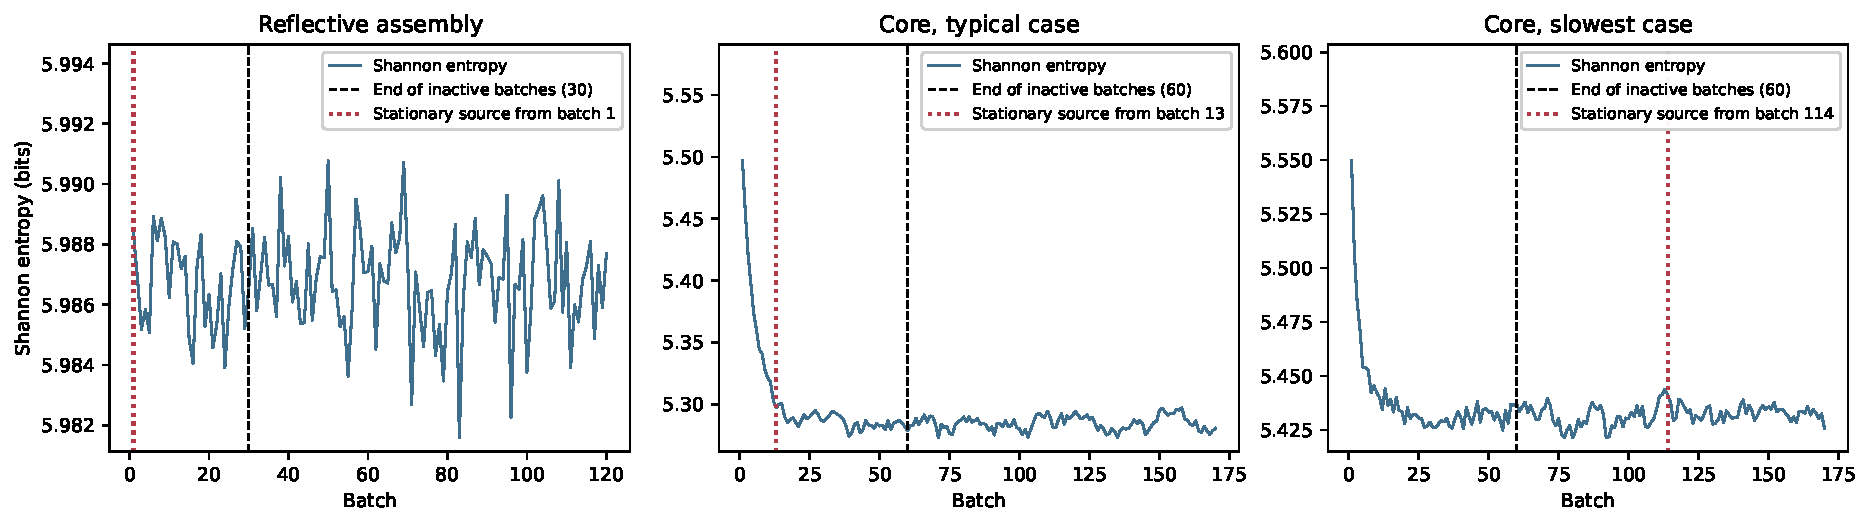
\includegraphics[width=\textwidth]{images/th_entropy.pdf}
          \caption{Shannon entropy per batch: reflective assembly, typical core solve and slowest core solve.}
          \label{fig:entropy}
        \end{figure}

  \item \textbf{Computing environment:} Table~\ref{tab:host-specs}
        gives the processor, memory, operating system and campaigns of
        each host. Both hosts run the same Conda environment, defined in
        the repository, with Python 3.13.13, OpenMC 0.15.3,
        pymoo 0.6.2 and scikit-learn 1.9.0.

\begin{table}[htbp]
  \centering
  \small
  \caption{Computing hosts: configuration and campaigns.}
  \label{tab:host-specs}\label{tab:hosts}
  \begin{tabularx}{\textwidth}{@{}l>{\raggedright\arraybackslash}X>{\raggedright\arraybackslash}X@{}}
    \toprule
    Characteristic & Cloud instance & Workstation \\
    \midrule
    Machine & AWS EC2 c7a.8xlarge, on demand & wks720 \\
    Processor & AMD EPYC 9R14, fourth generation (Genoa) & AMD Ryzen Threadripper 2990WX (Zen+, 12\,nm) \\
    Physical cores & 32 & 32 \\
    Logical processors & 32, simultaneous multithreading disabled & 64, two per core \\
    Clock frequency & Up to \SI{3.7}{GHz} & \SI{3.0}{GHz} base, \SI{4.2}{GHz} boost \\
    Memory & \SI{64}{GiB} & \SI{62}{GiB} available to the operating system \\
    Operating system & Ubuntu Server 24.04, Docker container & Linux Mint 22, kernel 6.8 \\
    Environment & Docker image with the pinned Conda environment & Pinned Conda environment, no administrative privileges \\
    Campaigns & 1, 2, 6 and 7 & 3 to 5, 8 and 9 \\
    \bottomrule
  \end{tabularx}
\end{table}

  \item \textbf{Sources of randomness:} three enter a campaign, and they
        differ in whether they are seeded.

        \begin{enumerate}
          \item Each transport solve is seeded from its own design
                vector (Section~\ref{sec:meth-fidelity}), so every
                archived design reproduces its result.

          \item The Gaussian-process hyperparameter optimisation and
                the NSGA-II search on the surrogate are seeded, so the
                same archive yields the same infill batch.

          \item The Latin-hypercube design of experiments is not
                seeded. The sampling routine of the framework declares a
                seed argument but never forwards it to the pymoo
                Latin-hypercube operator, which is therefore constructed
                without one and samples from the global state of the
                NumPy generator. Three launches with the same configured
                seed returned three different initial design matrices.
                The same routine generates the space-filling designs
                that complete a batch when the sequential selection
                under the minimum-distance constraint
                $\delta_\mathrm{min}$ of the batch-diversity revision
                of Section~\ref{sec:meth-acq} exhausts the candidates,
                so those points are not reproducible either.
        \end{enumerate}

        A campaign relaunched from scratch therefore starts from a
        different design of experiments and follows a different
        trajectory. The record of each campaign is its archived
        checkpoint, which stores every evaluated design with its inputs,
        outputs and the fixed hypervolume reference point, and every
        result of Chapter~\ref{ch:results} is computed from it. The
        checkpoints are held in the public code repository of this
        thesis, described in
        Appendix~\ref{app:code-architecture}. The
        surrogate-search study of Section~\ref{sec:meth-nsga-setting} is
        not affected, because it starts from a fixed archive and uses
        only the seeded search.
\end{itemize}


%% labels of the material reported with the campaign costs in the results, kept so that the
%% cross-references of the other chapters still resolve
\label{sec:meth-cost}

%% labels of the material summarised in the reactor model, kept so that the
%% cross-references of the other chapters still resolve
\label{sec:meth-dep-level}\label{eq:t-solve}\label{eq:t-solve-fit}\label{eq:t-step}\label{eq:bateman-asm}\label{eq:t-step-core}\label{tab:dep-level-cost}\label{tab:dep-3d-cost}



% =====================================================================
%  results.tex  --  Chapter 5 (Results and Discussion, to date)
%  Requires: booktabs, amsmath, graphicx.
%  Figures: figs_thesis/th_*.pdf (generator committed) plus the
%  campaign-generated figs/envelope_b2.pdf, gd_patterns.pdf,
%  figs_c3/corrected_front.pdf already in the repository.
%  \openpoint boxes mark work in progress -- delete as items close.
% =====================================================================
\providecommand{\openpoint}[1]{\par\noindent\fbox{\parbox{0.97\linewidth}{%
  \textbf{Open point:} #1}}\par}

\chapter{Results and Discussion}
\label{ch:results}

\section{Campaigns 1 and 2: the shakedown and the estimator}
\label{sec:res-c1c2}

The first two campaigns were executed on cloud infrastructure before
the workstation of Section~\ref{sec:meth-diagnostics} became available.
Their complete evaluation archives, execution logs and container
environment were recovered from the original instance and committed to
the repository, so every number reported here is reproduced from the
recovered checkpoints rather than from contemporaneous notes.
Table~\ref{tab:c1c2-provenance} records the execution provenance of
both campaigns.

\begin{table}[htbp]
  \centering
  \caption{Execution record of Campaigns 1 and 2, reconstructed from
  the recovered checkpoints and solver logs.}
  \label{tab:c1c2-provenance}
  \begin{tabular}{lcc}
    \toprule
    & Campaign 1 & Campaign 2 \\
    \midrule
    Execution window (2026)      & 10 July, single run & 12 to 13 July, resumed \\
    Host                         & \multicolumn{2}{c}{AWS EC2 c7a.8xlarge} \\
    Processor                    & \multicolumn{2}{c}{AMD EPYC 9R14, 32 physical cores} \\
    Execution environment        & \multicolumn{2}{c}{Docker image, pinned Conda} \\
    Transport code               & \multicolumn{2}{c}{OpenMC 0.15.3, ENDF/B-VII.1} \\
    Transport settings           & \multicolumn{2}{c}{$4\,000 \times 60$ (20 inactive)} \\
    $k$-target model             & interpolant in $t_\mathrm{refl}$ & tabulated calibration \\
    Constraint set               & 4 (no $g_\mathrm{geom}$) & 5 (with $g_\mathrm{geom}$) \\
    Depletion schedule           & fixed, 14 states & adaptive, 10 to 28 states \\
    Depletion horizon [MWd/kgHM] & 35.5 (implied) & 100.0 \\
    Real evaluations             & 72 & 84 (54 + 30) \\
    Transport solves             & 1008 & 2184 \\
    Evaluations at the horizon   & 39 (54.2\%) & 50 (59.5\%) \\
    Wall clock [h]               & 9.7 & 12.2 (resumed block) \\
    \bottomrule
  \end{tabular}
\end{table}

\subsection{Campaign 1: two structural findings}
\label{sec:res-c1}

Campaign 1 sampled the full design space of
Table~\ref{tab:design-space} at screening fidelity and completed 72
evaluations in a single 9.7 hour run, with the transport solver
accounting for 86\% of the wall clock at a mean of 29.7 seconds per
state solve. It produced 46 feasible designs. The 26 rejections are
distributed as follows.

\begin{enumerate}
  \item 25 designs violate $g_{k\max}$, the upper reactivity bound
        $k_\mathrm{BOL} \le 1.35$.
  \item 1 design violates $g_\mathrm{peak}$, the peaking screening
        bound $F_{\Delta H} \le 2.0$.
  \item No design violates $g_{k\min}$ or $g_\mathrm{enr}$.
\end{enumerate}

The campaign is retained in the record for two structural findings
rather than for its front.

The first finding is geometric. All four designs of the final Pareto
front carry reflector thicknesses between 23.99 and 24.99\,cm, whereas
the analytic vessel envelope admits at most 19.5\,cm even at the most
favourable pitch. Every nominally optimal design therefore exceeds the
vessel budget by at least 4.5\,cm. The optimiser exploited the one
physical requirement that the constraint set did not encode, and the
geometry constraint $g_\mathrm{geom}$ of Table~\ref{tab:constraints}
has been enforced inside the optimiser ever since
(Eq.~\ref{eq:renv}).

The second finding was silent at the time and emerged only from the
recovered archive. The depletion horizon of the evaluator maps onto a
cycle-length cap through the constant specific power,

\begin{equation}
  t_\mathrm{hor} = \frac{B_\mathrm{hor}}{P_\mathrm{spec}}
  \label{eq:depletion-horizon}
\end{equation}

\begin{itemize}
  \item $t_\mathrm{hor}$ is the maximum reportable cycle length, in
        effective full power days (EFPD).

  \item $B_\mathrm{hor}$ is the depletion horizon of the evaluator, in
        MWd/kgHM.

  \item $P_\mathrm{spec} = 9.983 \times 10^{-3}$\,MW/kgHM is the
        specific power of Table~\ref{tab:model-operating}.
\end{itemize}

In Campaign 1 the horizon was the evaluator default. Inverting
Equation~\eqref{eq:depletion-horizon} with the observed cap of
3555.9\,EFPD gives $B_\mathrm{hor} = 35.5$\,MWd/kgHM. Of the 72
evaluations, 39 (54.2\%) terminated exactly at this value, carrying an
identical, right-censored cycle-length entry
(Figure~\ref{fig:c1-front}a, where they are stacked on the implied
35.5\,MWd/kgHM depletion horizon and the four-design Pareto front is
marked). Among the censored designs the objective
is degenerate, so dominance within that majority subset is decided by
the peaking factor alone. The resolved designs span 610.6 to
3555.9\,EFPD with peaking factors between 1.136 and 2.207.

\begin{figure}[htbp]
  \centering
  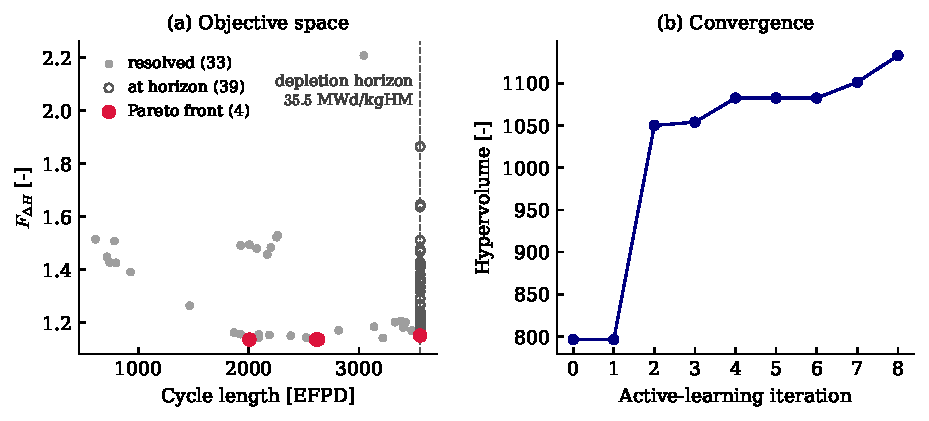
\includegraphics[width=\textwidth]{images/th_c1_front.pdf}
  \caption[Campaign 1 from the recovered checkpoint]{Campaign 1 from the recovered checkpoint. (a)~Objective space. (b)~Hypervolume history over the nine recorded active-learning iterations, reference point $(-1787.5,\ 1.785)$.}
  \label{fig:c1-front}
\end{figure}

\subsection{Campaign 2: the horizon test and the estimator}
\label{sec:res-c2}

Campaign 2 corrected both defects of the shakedown deliberately and
added the tabulated $k$-target calibration, the adaptive depletion
schedule and the geometry constraint. It raised the depletion horizon
from 35.5 to 100\,MWd/kgHM, a factor of 2.8, and completed 84
evaluations in two blocks, a 54-evaluation design of experiments and a
checkpoint-resumed block of five infill iterations of six points.

The horizon increase functioned as an unplanned experiment. The
censored fraction moved from 54.2\% to 59.5\%, essentially unchanged,
and all 50 censored designs again report the identical converted
horizon of 10016.7\,EFPD. The closest resolved design terminated at
10008.3\,EFPD, within 0.08\% of the cap. Tripling the horizon therefore
did not resolve the objective. The degeneracy is generated by the
design space itself, in which enrichments approaching the LEU cap
combined with thick reflectors carry a reactivity inventory that
sustains criticality far beyond any operationally meaningful cycle.
The remedy adopted from Campaign 3 onward is the physically grounded
discharge limit of Section~\ref{sec:meth-atf}, enforced inside the
depletion loop, which converts the arbitrary horizon into a
design-basis bound and eliminates censoring by construction.

The entries at the horizon carry no design meaning. The reported
refuelling interval of five years corresponds to 913 to 1461
EFPD at capacity factors between 0.5 and 0.8
(Section~\ref{sec:res-c8-mission}), so a cycle length of several
thousand days exceeds the mission by a factor of five to ten. Such a
design carries at beginning of life a reactivity inventory that the
controllability screen of Section~\ref{sec:meth-ctrl} later shows to
be beyond the regulating banks, and the horizon values measure that
inventory rather than describe a credible core.

Campaign 2 also exposed the estimator pathology
(Table~\ref{tab:c2-summary}). The stored single-seed peaking values
carried a bias larger than the front spread they ranked, and resolving
the candidates at high fidelity inverted the ranking. The stored fourth
became the true first, the apparent winner fell to seventh, and the
pair separated at $|t| = 12.8$. The statistical treatment that this
finding forced, per-design seeding, the fidelity ladder and two-stage
subset selection, is specified in Sections~\ref{sec:meth-fidelity}
and~\ref{sec:meth-stats}.

\begin{table}[htbp]
  \centering
  \caption{Campaign 2 in five numbers.}
  \label{tab:c2-summary}
  \begin{tabular}{lc}
    \toprule
    Uncapped front span, EFPD / $F_{\Delta H}$ & 17.7\% / 5.1\% \\
    Seed-to-seed s.d.\ of $F_{\Delta H}$ (stored fidelity) & up to 0.018 \\
    Bias of the stored values vs 256k reference & $-0.07$ \\
    Ranking outcome after resolution & inverted (4th $\to$ 1st) \\
    Corrected 75\,MWd/kgHM front & 2 designs (trade-off restored) \\
    \bottomrule
  \end{tabular}
\end{table}

The seed-to-seed standard deviation in Table~\ref{tab:c2-summary} comes
from a replication of the three lowest-peaking front designs at the
stored fidelity of $4\,000\times60$, with five seeds each. The
per-design values are 0.018, 0.007 and 0.018, and the pooled value is
$0.015\pm0.003$.

\subsection{Hypervolume comparability across campaigns}
\label{sec:res-hv-comparability}

The recovered archives fix the hypervolume reference points of the
early campaigns at $(-1787.5,\ 1.785)$ for Campaign 1 and
$(-5063.4,\ 1.976)$ for Campaign 2, in signed objective space. The
reference points differ on both axes, and the objective definition
itself changed when the discharge limit entered the cycle-length
objective. Hypervolume magnitudes are therefore not comparable across
campaigns, and none are compared in this work. Each history is read
only for its internal convergence shape, consistent with the reset
policy of Section~\ref{sec:meth-atf}. Any future cross-campaign figure
must first recompute all histories against a single reference point
taken as the componentwise worst value over the union of the archives,
a pure post-processing step on the committed checkpoints.

\openpoint{Pin the exact Campaign 1 code state (one of the four
commits of 10 July 2026) and the step list of the default depletion
schedule by inspecting the evaluator at that commit. Verify the
Campaign 2 feasible count of 44 directly from the recovered checkpoint
before the viva.}

% ============================ end of drop-in ==========================

\section{Campaign 3: design of experiments and feasibility envelope}
\label{sec:res-c3doe}

Campaign 3 (72 evaluations at $16\,000\times120$, per-design seeds, ATF
limit in-loop) opens with a 36-point Latin hypercube: 11 feasible
(31\%), with the upper reactivity bound responsible for 21 of 25
rejections. Regression over the archive gives the feasibility envelope
($R^2 = 0.92$--$0.94$, stable from $n=36$ to $n=72$):
\begin{equation}
  k_\mathrm{BOL} \;=\; 0.894 \;+\; 0.215\,\ln e_\mathrm{vw}
  \;-\; 0.0066\,\mathrm{gd},
  \qquad
  e_\mathrm{vw} = 0.72\,e_\mathrm{out} + 0.28\,e_\mathrm{in}.
  \label{eq:envelope}
\end{equation}

Three readings of Eq.~\eqref{eq:envelope} organise the design space.
Volume-weighted enrichment governs: the 72/28 zone split makes
$e_\mathrm{out}$ dominant by construction. Gadolinium at the fixed
twelve-pin pattern buys only $\Delta k \approx 0.05$--$0.06$ over its
full range, which is 2.7\,wt\% of enrichment headroom, against layouts
of up to 40 poisoned pins per assembly studied for soluble-boron-free
cores~\cite{rr_smr_atf_2025,ismr_sbf_2024}. And pitch emerges as the
second feasibility lever (logistic coefficient $+1.67$ at $n=72$,
behind only $e_\mathrm{out}$): over-moderation reaches criticality at
low enrichment. The envelope figure generated from the archive
(\texttt{figs/envelope\_b2}) belongs here.

\section{Campaign 3: convergence and the resolved front}
\label{sec:res-c3front}

Figure~\ref{fig:hv} shows the hypervolume of Campaign 3. Block 1 delivers
the gains, and Block 2 returns three consecutive exact zeros, so the
stopping rule is met with margin.

\begin{figure}[htbp]
  \centering
  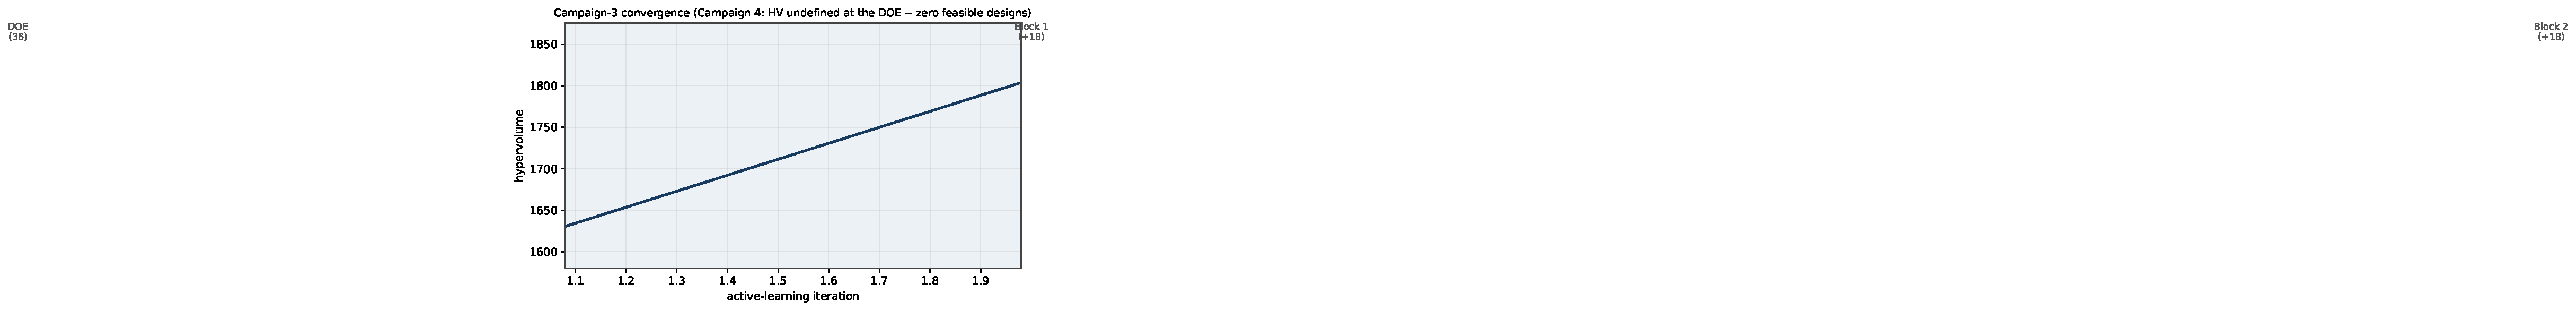
\includegraphics[width=0.86\linewidth]{images/th_hv_history}
  \caption{Campaign 3 hypervolume.}
  \label{fig:hv}
\end{figure}

Block behaviour carries information beyond the trajectory
(Fig.~\ref{fig:hv}): Block-1 infill was \textbf{18/18 feasible} against
the DOE's 31\%, because the surrogate had learned the reactivity
boundary, and only 6/18 at the burnup cap, walking into the below-cap region where
a trade-off exists. Block 2 (7/18 feasible, 18/18 at the cap) probed
the constraint boundary of an already-stable front: the signature of
convergence seen from inside.

High-fidelity resolution ($256\,000\times8$ seeds,
Fig.~\ref{fig:plateau}) then reshapes the stored front
(Table~\ref{tab:c3-resolved}). The shifts are design-dependent, from
$-0.003$ to $-0.020$, and the four plateau members are pairwise
unresolved. The design-dependent bias re-orders the set a second time,
after Campaign 2.

\begin{table}[htbp]
  \centering
  \caption{Campaign 3 finalists after high-fidelity resolution.}
  \label{tab:c3-resolved}
  \begin{tabular}{lcccc}
    \toprule
    & stored & measured (95\% CI) & shift & EFPD \\
    \midrule
    cand2 & 1.1336 & $1.1212\pm0.0021$ & $-0.0124$ & 5\,239 \\
    cand0 & 1.1266 & $1.1213\pm0.0019$ & $-0.0053$ & 5\,180 \\
    cand5 & 1.1445 & $1.1241\pm0.0010$ & $-0.0204$ & 5\,902 \\
    cand1 & 1.1270 & $1.1244\pm0.0010$ & $-0.0026$ & 2\,904 \\
    \midrule
    cand6 & 1.1483 & $1.1291\pm0.0023$ & $-0.0192$ & 5\,358 \\
    cand7 (capped) & 1.1522 & $1.1319\pm0.0038^{\dagger}$ & --- & 7\,513 \\
    cand3 (capped) & 1.1397 & $1.1381\pm0.0037^{\dagger}$ & --- & 7\,513 \\
    \bottomrule
    \multicolumn{5}{l}{\footnotesize $^{\dagger}$64k measurement,
    bias-adjusted to 256k; cand7 beats cand3 at $|t|=3.38$ (measured).}
  \end{tabular}
\end{table}

\begin{figure}[htbp]
  \centering
  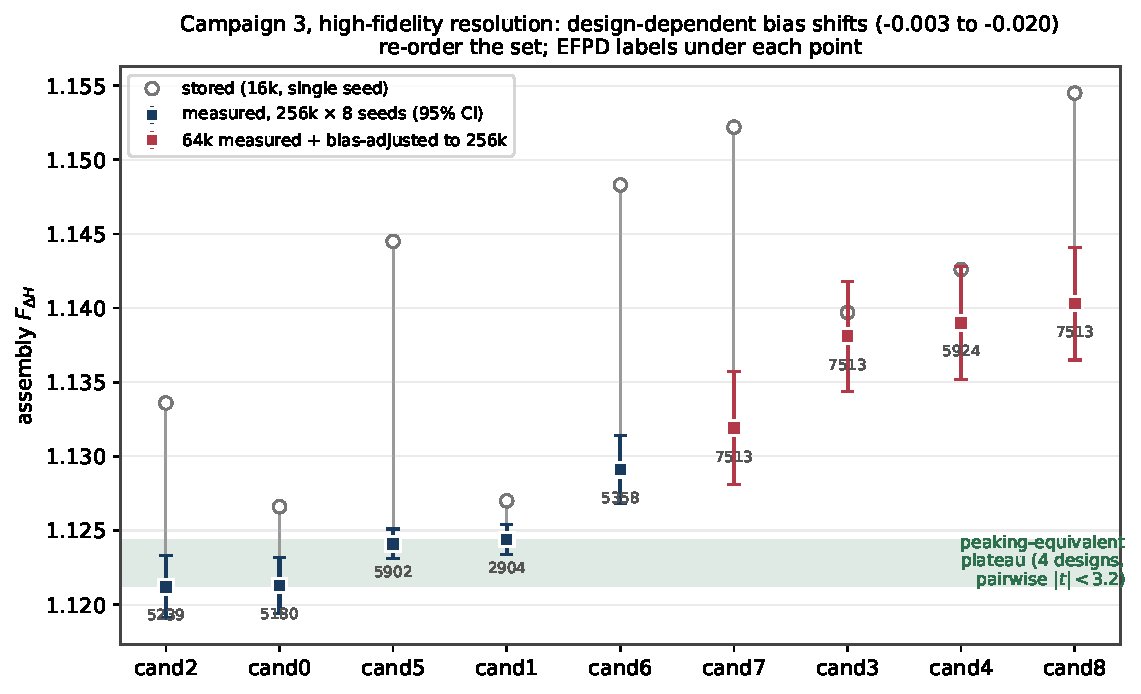
\includegraphics[width=0.9\linewidth]{images/th_c3_plateau}
  \caption{Stored versus resolved peaking of the Campaign 3 finalists.}
  \label{fig:plateau}
\end{figure}

The assembly-level result is therefore \textbf{a plateau, not a
winner}: four designs statistically identical in $F_{\Delta H}$
(1.1212--1.1244) spanning 2\,904--5\,902\,EFPD, plus the capped
strategy at 7\,513\,EFPD led by cand7, which is itself not separated
from the plateau once bias-adjusted ($|t|=2.6$). Two engineering strategies
emerge: a thick-reflector, high-enrichment capped design pressed
against the vessel ($g_\mathrm{geom}=-0.4$\,cm), and an over-moderated
cluster (pitch 1.41, enrichment $\sim$5.3\,wt\%, thin reflector).
Both are shaped by the same scarce resource, the 90\,cm vessel radius
(Eq.~\ref{eq:renv}).
%% AUTHOR: 2-3 sentences of physics on the two strategies (reflector
%% leakage vs over-moderation; MTC risk of the wide-pitch cluster).

\section{Core-level validation: the proxy gap}
\label{sec:res-corevalidation}

Rebuilding the finalists as full cores (BOL, 8 seeds) measures what the
reflective assembly cannot see (Table~\ref{tab:core-finalists}).

\begin{table}[htbp]
  \centering
  \caption{Campaign 3 finalists at core level ($100\,000\times$ up to 230 batches, 8 seeds).}
  \label{tab:core-finalists}
  \begin{tabular}{lcccc}
    \toprule
    & $F_{\Delta H}^\mathrm{asm}$ & $F_{\Delta H}^\mathrm{core}$
      (95\% CI) & ratio & EFPD \\
    \midrule
    idx46 (cand3) & 1.1397 & $2.013\pm0.018$ & 1.77 & 7\,513 \\
    idx45 (cand7) & 1.1522 & $2.020\pm0.019$ & 1.75 & 7\,513 \\
    idx53 (cand5) & 1.1445 & $2.114\pm0.018$ & 1.85 & 5\,902 \\
    \bottomrule
  \end{tabular}
\end{table}

Three facts. The proxy gap is a factor \textbf{1.75--1.91},
anti-correlated with reflector thickness ($r=-0.96$ over the six
finalists): thin reflectors leak, depress the periphery, and drive
core-wide peaking, an effect invisible to an infinite lattice. The ranking
\emph{inverts}: the assembly-best design is core-worst, and the capped
pair (idx46/idx45, tied at $|t|=0.54$) beats the plateau at
$|t|\approx7$--$8$, collapsing the front to the capped strategy. And the
peaking constraint, inactive everywhere at assembly level, is now
\textbf{violated by every design}: the best sits at
$2.013\pm0.018$ against the 2.0 limit.

Rescoring the \emph{entire} feasible archive (36 designs,
Fig.~\ref{fig:asmcore}) generalises the finding. The proxy is globally
informative, with $\rho=+0.890$, yet scrambles the ordering exactly where
the optimiser operates. Table~\ref{tab:proxy-numbers} gives the proxy in
numbers and the designs it mis-ranked, with rank positions taken among
the 36 feasible Campaign 3 designs.

\begin{figure}[htbp]
  \centering
  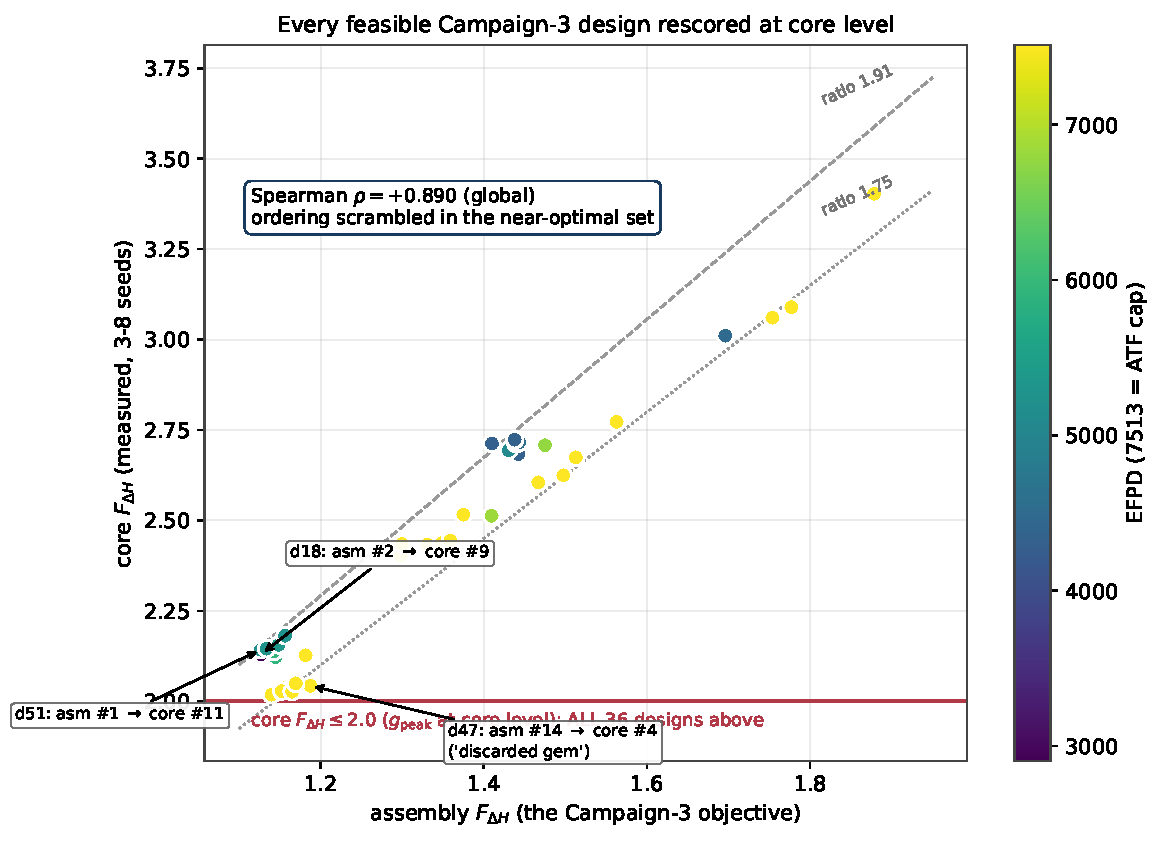
\includegraphics[width=0.9\linewidth]{images/th_asm_vs_core}
  \caption{Every feasible Campaign 3 design rescored at core level.}
  \label{fig:asmcore}
\end{figure}

\begin{table}[htbp]
  \centering
  \small
  \caption{The proxy in numbers, and the designs it mis-ranked.}
  \label{tab:proxy-numbers}
  \begin{tabularx}{\textwidth}{@{}>{\raggedright\arraybackslash}p{0.48\textwidth}>{\raggedright\arraybackslash}X@{}}
    \toprule
    Quantity & Value \\
    \midrule
    Spearman $\rho$, assembly versus core, $n=36$
      & $+0.890$ \\
    Assembly ranks 1 / 2 / 3, re-evaluated at core level
      & 11 / 9 / 12 \\
    Largest rank gains, the discarded gems
      & d47: \#14 $\to$ \#4 \newline
        d43: \#9 $\to$ \#2 \newline
        d42: \#11 $\to$ \#5 \\
    Core-level Pareto front
      & A single design, d46, violating $F_{\Delta H}\le 2.0$ \\
    Designs meeting $F_{\Delta H}^\mathrm{core}\le 2.0$
      & 0 of 36 \\
    \bottomrule
  \end{tabularx}
\end{table}

The bridge model (Eq.~\ref{eq:bridge}) fitted on all 36 designs,
\begin{equation}
  \frac{F^\mathrm{core}}{F^\mathrm{asm}}
  = 1.400 \;-\; 0.0045\,t_\mathrm{refl} \;+\; 0.343\,p,
  \qquad R^2 = 0.746,
  \label{eq:bridge-fit}
\end{equation}
confirms reflector and pitch as the corrupting variables, and its
residual quarter is the argument for measuring rather than correcting.
The fit describes the uniform loading of Campaign~3 only. On the zoned
core that the evaluator builds from Campaign~6 the ratio is smaller and
no longer depends on the geometry, as
Section~\ref{sec:res-proxy-gap-zoned} reports.

Route-B closure on the finalists gives residuals of $-91$ to
$-429$\,pcm (most negative for thick reflectors), validating the
cycle-length proxy at the $\sim$2\% level, and the Shannon-entropy
diagnostic of the core solves identified one case converging at batch 94 against a 40-batch
cutoff, which is the reason the production core solves carry 60 to 120
inactive batches.

\textbf{The methodological statement of the thesis follows:} a
surrogate-assisted optimisation on a reduced-order proxy must validate
the proxy's \emph{rank fidelity} near the optimum, not merely its
statistical convergence, because correlation weakens exactly where the
optimiser converges, and it did so here twice (estimator bias in
Campaign 2, geometric proxy in Campaign 3).

\section{Campaign 4: the core-level objective}
\label{sec:res-c4}

Campaign 4 moves $F_{\Delta H}$ and $g_\mathrm{peak}$ to core level at
$\approx3\%$ evaluation cost (Eq.~\ref{eq:corecost}) and is complete:
a 36-point DOE plus three infill iterations of six evaluations each,
54 designs in total, \textbf{zero feasible}
(Table~\ref{tab:c4-doe}, Fig.~\ref{fig:c4traj}). With an empty feasible set
the hypervolume is undefined and is reported as zero, so convergence is
judged on the reduction of the constraint violation.

\begin{table}[htbp]
  \centering
  \caption{Campaign 4 design of experiments against that of Campaign 3, with the same limits and design space.}
  \label{tab:c4-doe}
  \begin{tabular}{lcc}
    \toprule
    & C3 DOE (assembly $g_\mathrm{peak}$) & C4 DOE (core
      $g_\mathrm{peak}$) \\
    \midrule
    feasible                     & 11 / 36 & \textbf{0 / 36} \\
    $g_\mathrm{peak}$ violations & 4       & \textbf{35} \\
    $g_{k\max}$ violations       & 21      & 24 \\
    best $F_{\Delta H}$ (its level) & 1.127 & 1.9215 \\
    \bottomrule
  \end{tabular}
\end{table}

\begin{figure}[htbp]
  \centering
  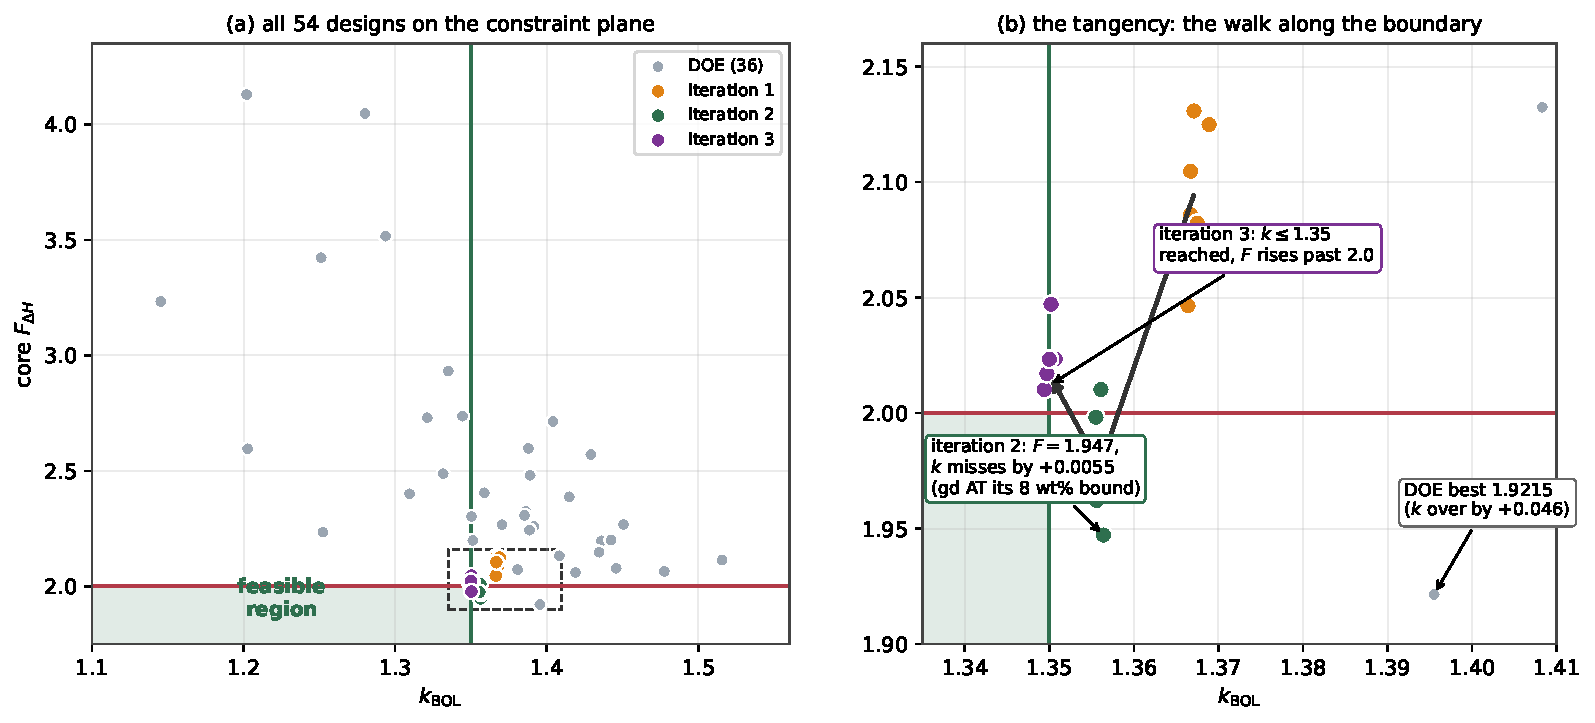
\includegraphics[width=\linewidth]{images/c4_trajectory}
  \caption[Campaign 4 on the constraint plane]{Campaign 4 on the constraint plane. (a)~All 54 designs. (b)~The three-iteration walk along the boundary.}
  \label{fig:c4traj}
\end{figure}

\subsection{Infill trajectory and the tangency of the feasible region}
\label{sec:res-c4-trajectory}

The infill ran under constraint-violation ranking throughout, since no
design was ever feasible. Its trajectory
(Table~\ref{tab:c4-trajectory}) is the campaign's central measurement. The
total violation reaches its minimum at iteration 2 and rises again at
iteration 3, when $k_\mathrm{BOL}\leq1.35$ is finally satisfied.

\begin{table}[htbp]
  \centering
  \caption{Campaign 4 infill iterations: ranges over the six designs of each iteration.}
  \label{tab:c4-trajectory}
  \begin{tabular}{ccccc}
    \toprule
    iteration & $k_\mathrm{BOL}$ & core $F_{\Delta H}$ &
      mean total violation \\
    \midrule
    DOE  & 1.145 -- 1.516 & 1.921 -- 4.129 & 0.084 \\
    1    & 1.3664 -- 1.3689 & 2.046 -- 2.131 & 0.1131 \\
    2    & 1.3555 -- 1.3567 & \textbf{1.947} -- 2.010 & \textbf{0.0077} \\
    3    & \textbf{1.3494} -- 1.3507 & 1.977 -- 2.047 & 0.0204 \\
    \bottomrule
  \end{tabular}
\end{table}

Three facts define the outcome. The optimiser collapsed the reactivity
spread by a factor of 200 (DOE $k_\mathrm{BOL}$ standard deviation
0.081; iteration-1 spread 0.0025) and then walked $k_\mathrm{BOL}$
down through the limit across iterations. Iteration 2 achieved
designs feasible on peaking ($F_{\Delta H}=1.947$--$2.010$) missing
only the reactivity limit, by $+0.0055$ to $+0.0067$. Iteration 3
satisfied the reactivity limit ($k_\mathrm{BOL}=1.3494$--$1.3507$) and
lost peaking feasibility in exchange.

The two constraints are therefore \textbf{tangent, not overlapping},
within this five-variable space: each is satisfiable alone, their
intersection was never reached, and the converged residual gap is
$\Delta k \approx 0.006$ measured at the point of closest approach.

\subsection{Exhaustion of the design space at a vertex}
\label{sec:res-c4-vertex}

Figure~\ref{fig:c4parallel} shows the Campaign 4 designs in parallel
coordinates by phase, with the design of experiments in grey filling the
box.

\begin{figure}[htbp]
  \centering
  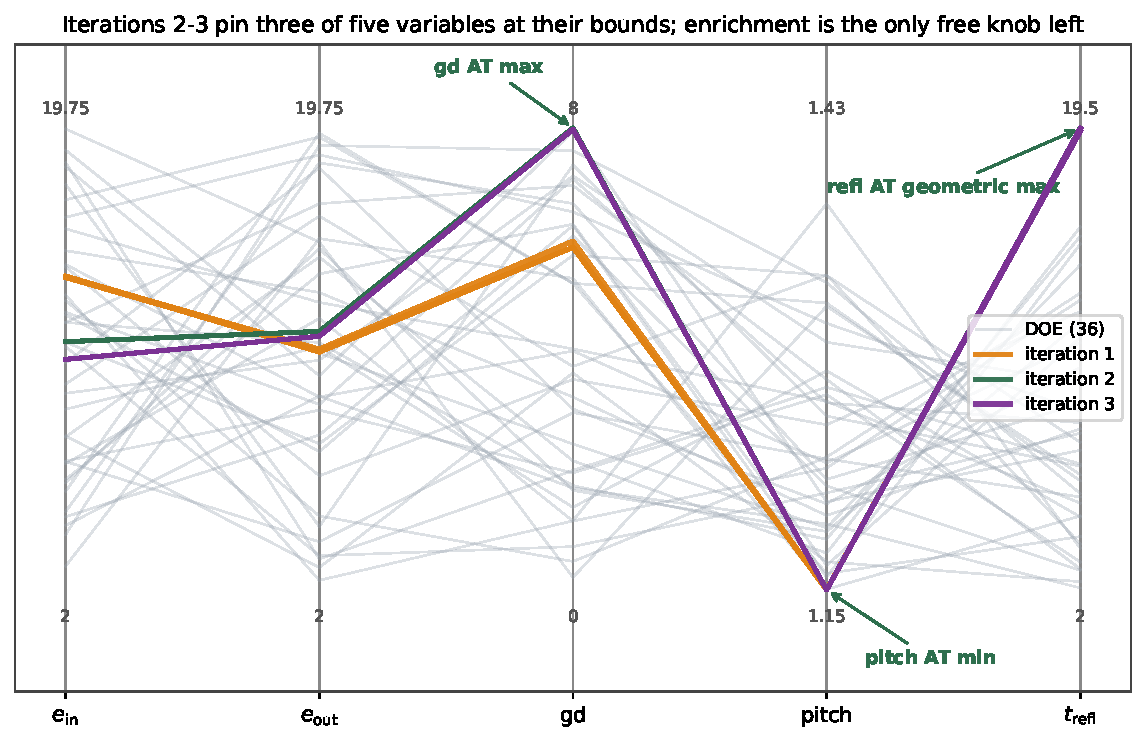
\includegraphics[width=0.92\linewidth]{images/c4_parallel}
  \caption{Campaign 4 design variables in parallel coordinates by phase.}
  \label{fig:c4parallel}
\end{figure}

Every iteration-2 and iteration-3 design pins \textbf{three of the five
variables at their bounds} (Fig.~\ref{fig:c4parallel}): gadolinium
concentration at 8.0\,wt\% (to four decimals), pitch at 1.150\,cm, and
reflector thickness at the vessel-budget ceiling
(Eq.~\ref{eq:renv}). The sole remaining degree of freedom, enrichment,
is what the optimiser walks: $e_\mathrm{vw}=11.82$\,wt\% at iteration 2
to $11.50$\,wt\% at iteration 3. That slide \emph{is} the
$k_\mathrm{BOL}$ descent of Table~\ref{tab:c4-trajectory}.

The constrained optimum of Campaign 4 therefore sits at a vertex of the
design box, and the optimiser is, in effect, requesting more absorber
than the concentration bound permits. The identified resolution,
absorber \emph{inventory} as a variable, follows in
Section~\ref{sec:res-campaign5}.

The pitch bound reached at iterations 2 and 3 carries the geometric
caveat established later in this work. Below \SI{1.2242}{cm} the
lattice clips the guide-tube wall silently, so the eigenvalues and the
peaking values of the \SI{1.150}{cm} designs of this campaign are
biased by an unquantified amount
(Section~\ref{sec:res-c7-limits}).

\subsection{Variable influence and the champion designs}
\label{sec:res-c4-champions}

Figure~\ref{fig:c4influence} plots each design variable against the core
peaking factor over all 54 designs. Volume-weighted enrichment dominates,
with $r=-0.59$, and $-0.63$ for $e_\mathrm{out}$ alone. Gadolinium is
peaking-neutral at $r=-0.16$, because it buys reactivity without
flattening the power, which is why the conflict is structural.

Figure~\ref{fig:c4objectives} shows the objective plane. With 46 of 54
designs at the 75\,MWd/kgHM cap the trade-off degenerates. The
unconstrained non-dominated set is a single infeasible capped design, and
the campaign is effectively a single-objective constrained minimisation
of core peaking. Table~\ref{tab:c4-champions} lists the champion designs.

\begin{figure}[htbp]
  \centering
  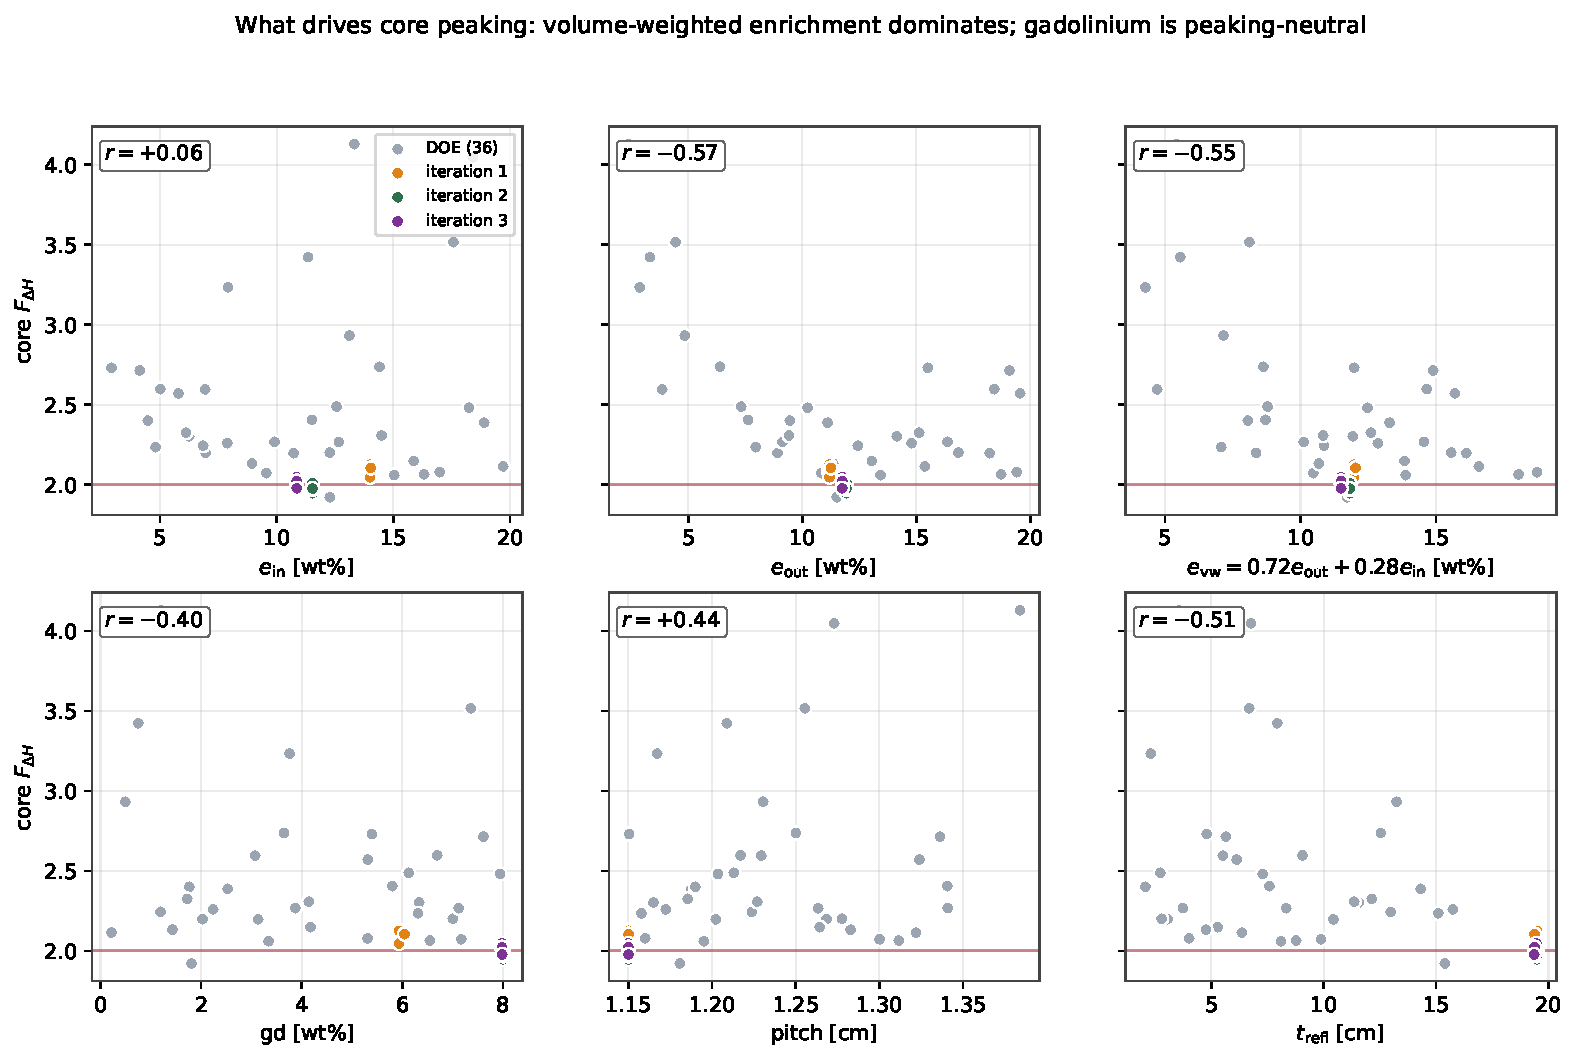
\includegraphics[width=\linewidth]{images/c4_influence}
  \caption{Campaign 4 design variables against core $F_{\Delta H}$, all 54 designs.}
  \label{fig:c4influence}
\end{figure}

\begin{figure}[htbp]
  \centering
  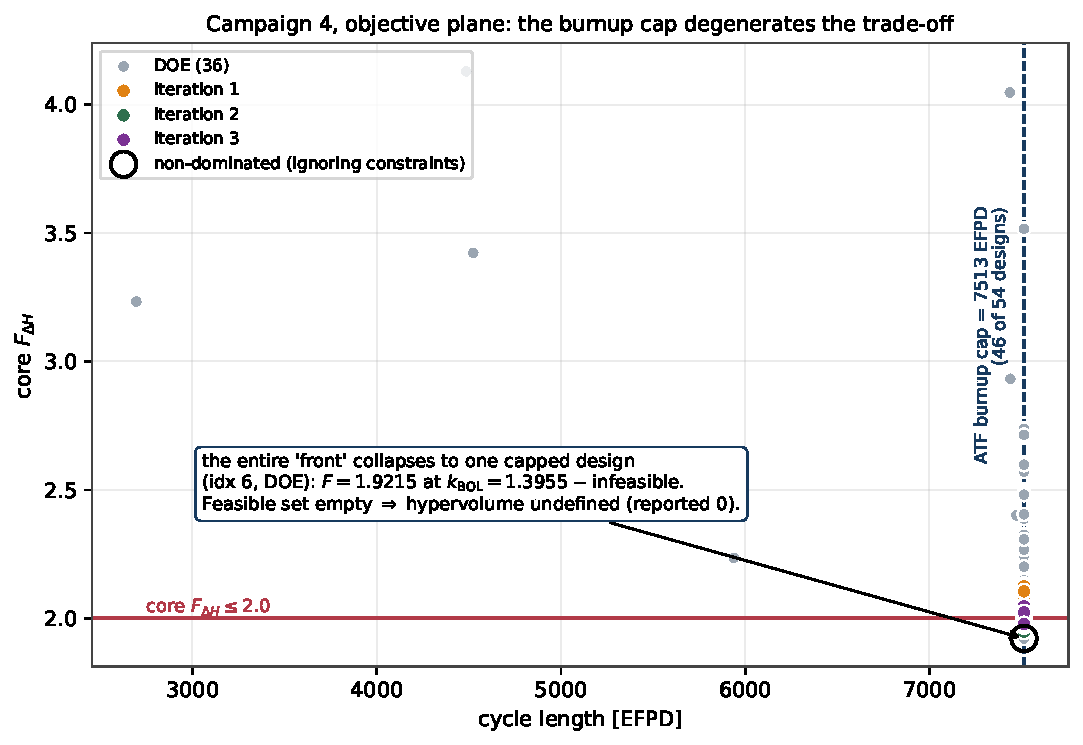
\includegraphics[width=0.9\linewidth]{images/c4_objectives}
  \caption{Campaign 4 objective plane.}
  \label{fig:c4objectives}
\end{figure}

\begin{table}[htbp]
  \centering
  \small
  \caption{The champion designs of Campaign~4. Bold marks a value
  sitting at a design-space bound.}
  \label{tab:c4-champions}
  \begin{tabularx}{\textwidth}{@{}>{\raggedright\arraybackslash}p{0.26\textwidth}*{3}{>{\centering\arraybackslash}X}@{}}
    \toprule
    Quantity & idx 6, DOE & idx 44, iteration 2 & Iteration 3, typical \\
    \midrule
    $e_\mathrm{in}$ / $e_\mathrm{out}$ [wt\%]
      & 12.28 / 11.50 & 11.54 / 11.93 & $e_\mathrm{vw} = 11.50$ \\
    Gd$_2$O$_3$ content [wt\%]
      & 1.81 & \textbf{8.00} & 7.98 \\
    Pitch [cm]
      & 1.181 & \textbf{1.150} & \textbf{1.150} \\
    $t_\mathrm{refl}$ [cm]
      & 15.39 & \textbf{19.49} & 19.35--19.48 \\
    Core $F_{\Delta H}$ [--]
      & \textbf{1.9215} & 1.9472 & 1.977--2.047 \\
    $k_\mathrm{BOL}$ [--]
      & 1.3955 & 1.3564 & 1.3494--1.3507 \\
    Status
      & Peaking met, $k_\mathrm{BOL}$ high by 0.046
      & Closest approach, $k_\mathrm{BOL}$ high by 0.0055
      & $k_\mathrm{BOL}$ met, peaking exceeded \\
    \bottomrule
  \end{tabularx}
\end{table}

Design idx 44 deserves one further remark: its reflector sits at
19.4914\,cm at pitch 1.150\,cm, exactly the corrected geometric
ceiling. The optimiser found the vessel-budget corner twice: once
illegally, through a 0.02\,cm inconsistency between the analytic
constraint and the geometry builder (crashing the first infill
attempt; the fix made the builder's fuel-envelope pad part of
$g_\mathrm{geom}$), and once legally, after the fix. Both episodes,
together with a mid-loop failure of the optimiser on an empty feasible
set (repaired by a least-infeasible infill fallback and per-iteration
checkpointing), are recorded in the methodology diagnostics: an
optimiser pressing on constraint boundaries is an adversarial
verification tool, and it found two real defects this way.
%% AUTHOR: 1-2 sentences of physics on WHY high enrichment flattens the
%% core radial profile (periphery-to-centre gradient, migration).

\section{Campaign 5: the absorber inventory as a design variable}
\label{sec:res-campaign5}

Campaign 4's converged residual is small and precisely located:
$\Delta k \approx 0.006$ at the iteration-2 champion, with the
concentration route closed by its own bound. Scaling the fitted 12-pin
authority (0.0525 in $\Delta k$ at 8\,wt\%) by inventory,
\begin{equation}
  \Delta k_\mathrm{pins}(n) \;=\; 0.0525\,\frac{n-12}{12}
  \;\;\Rightarrow\;\;
  n \;\approx\; 13.5 ,
  \label{eq:pins-needed}
\end{equation}

so \textbf{approximately two additional gadolinia pins} were predicted to
close the gap, a far smaller departure from the twelve-pin heritage pattern
than the DOE-based estimate of approximately 23 pins suggested before the
infill located the true point of closest approach. Campaign 5 was designed
to test that prediction by admitting the pin count as a search variable
rather than fixing it. Table~\ref{tab:c5} lists the changes relative to
Campaign 4, one of them structural to the search space, and the
disposition of each at the close of the campaign.

\begin{table}[htbp]
  \centering
  \small
  \caption[Campaign 5 relative to Campaign 4]{Campaign 5 relative to Campaign 4: changes and their disposition at the close of the campaign.}
  \label{tab:c5}
  \begin{tabularx}{\textwidth}{@{}>{\raggedright\arraybackslash}p{0.24\textwidth}>{\raggedright\arraybackslash}X>{\raggedright\arraybackslash}p{0.24\textwidth}@{}}
    \toprule
    Change & Rationale & Disposition \\
    \midrule
    Gd pin count as sixth design variable, 12 to 40 rods in
    octant-symmetric patterns
      & The optimiser exhausted the concentration bound
        (Fig.~\ref{fig:c4parallel}). Inventory scales absorber authority
        without the self-shielding penalty and is the primary lever
        reported in the literature at a fixed weight fraction of
        approximately 8\,wt\%~\cite{rr_smr_atf_2025}
      & Implemented. Minimum total constraint violation fell from 0.0077
        to 0.0012 (Fig.~\ref{fig:c5traj}) \\
    Single-design pin-count test on idx 44
      & Re-evaluation at 14, 16 and 20 rods to decide within hours
        whether the tangency opens
      & Executed. Feasibility reached at 14 rods,
        $k_\mathrm{BOL}=1.3456$, at a measured authority of
        approximately \SI{500}{pcm} per rod (Fig.~\ref{fig:c5pins}) \\
    Constraint normalisation by individual limits
      & The Campaign 1 to 4 violation sum added quantities in
        $\Delta k$, peaking factor, weight percent and centimetres
        without weighting
      & Implemented in Campaign 5 \\
    $g_{k\max}$ moved to core $k_\mathrm{eff}$
      & Excess reactivity is a core quantity, and
        $k_\mathrm{eff}^\mathrm{core}$ is already recorded per
        evaluation at no additional cost
      & Not applied during the search. Applied retrospectively to both
        archives in Section~\ref{sec:res-c5-kbasis}, where it admits
        exactly the designs the assembly screen admits at 1.40 \\
    Soluble-boron decision
      & Civil soluble-boron-free practice~\cite{ismr_sbf_2024,acp100_physor2020}
        motivates a boron-free basis. Removing the boron raises
        $k_\mathrm{BOL}$ by approximately 0.08 to 0.10,
        which tightens the problem rather than relaxing it
      & Closed. The \SI{1000}{ppm} benchmark-traceable basis of
        Section~\ref{sec:meth-boron} is retained for all campaigns, and
        the boron-free case is recorded as future work \\
    Review of the 1.35 bound
      & The limit proxies controllable excess reactivity without a rod
        model. At 1.40 both champions of
        Table~\ref{tab:c4-champions} are already feasible
      & Resolved by the re-scoring of Section~\ref{sec:res-c5-kbasis},
        which shows that the basis change and the relaxation to 1.40
        select identical design sets, and traced in Campaign 7 to the
        measured all-bank controllability bound of 1.368
        (Section~\ref{sec:res-c7-worth}) \\
    \bottomrule
  \end{tabularx}
\end{table}

The single-design test settles the Campaign 4 prediction before the
campaign results are examined. Re-evaluating the Campaign 4 champion at
14, 16 and 20 gadolinia rods measures an inventory authority of
approximately \SI{500}{pcm} per rod, so the two-rod step from 12 to 14
removes \SI{1011}{pcm} against the required \SI{640}{pcm}. The design is
feasible on both screening constraints at 14 rods, which confirms the
prediction of Equation~\eqref{eq:pins-needed} within one rod. The core
peaking factor is unchanged across the four counts, remaining between
1.970 and 1.995, so the inventory buys reactivity control and no peaking
penalty, consistent with the variable-influence finding of
Section~\ref{sec:res-c4-champions}.

In Figure~\ref{fig:c5pins} the assembly eigenvalue, left, crosses the
screening limit between 12 and 14 rods, and a fit over the four counts
gives an authority of \SI{535}{pcm} per rod. The core radial peaking
factor, right, is statistically flat across the four counts. The error
bars are one standard error of the mean.

\begin{figure}[htbp]
  \centering
  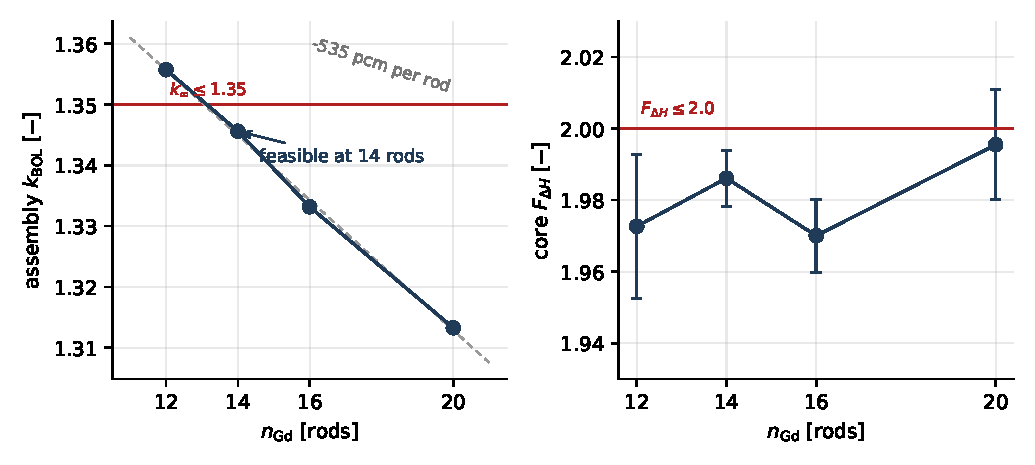
\includegraphics[width=0.95\linewidth]{images/c5_pin_worth}
  \caption[Pin-count test on the Campaign 4 champion]{Pin-count test on the Campaign 4 champion, archive index 44, at 12, 14, 16 and 20 gadolinia rods.}
  \label{fig:c5pins}
\end{figure}

\subsection{Search outcome under the as-run constraints}
\label{sec:res-c5-search}

Campaign 5 evaluated 60 designs, a 42-point Latin hypercube design of
experiments followed by three active-learning iterations of six real
evaluations each. The two blocks ran on consecutive days and the active
wall time was \SI{108.4}{\hour}, equal to 6934 core-hours, with the
complete cost decomposition recorded with the campaign checkpoint
(Appendix~\ref{app:code-architecture}).

The feasible set was empty at every recorded checkpoint. The hypervolume
history is identically zero at all four recorded points, the reference
point was never frozen because freezing requires a first feasible design,
and the empirical stopping rule of
Section~\ref{sec:res-hv-comparability} was therefore inoperative. The
campaign terminated on its iteration budget, not on convergence. Under an
empty feasible set the optimiser degrades to minimisation of the total
constraint violation
\begin{equation}
  V \;=\; \sum_{j} \max\!\left(0,\; \frac{g_j}{\lvert g_j^\mathrm{lim}
  \rvert}\right) ,
  \label{eq:violation-normalised}
\end{equation}

with the terms

\begin{itemize}
  \item $g_j$, the value of constraint $j$ in its native units,
  \item $g_j^\mathrm{lim}$, the limit of constraint $j$ in the same
        units, introduced as the per-constraint normalisation adopted in
        this campaign,
  \item $V$, the total normalised violation, dimensionless.
\end{itemize}

Figure~\ref{fig:c5traj} shows the resulting search trajectory, with the
running best as a step line. The design of experiments occupies indices
0 to 41, the three infill iterations follow in blocks of six, and the
three annotated designs are the champions discussed below. The best
design of experiments point reaches $V = 0.0264$ at archive index 17.
The first iteration does not improve on it, closing at $V = 0.0321$. The
second iteration reaches $V = 0.0074$ at index 49 and the third reaches
$V = 0.0012$ at index 54, the campaign champion. Relative to the best
Campaign 4 value of 0.0077, the sixth design variable moved the point of
closest approach by a factor of six.

\begin{figure}[htbp]
  \centering
  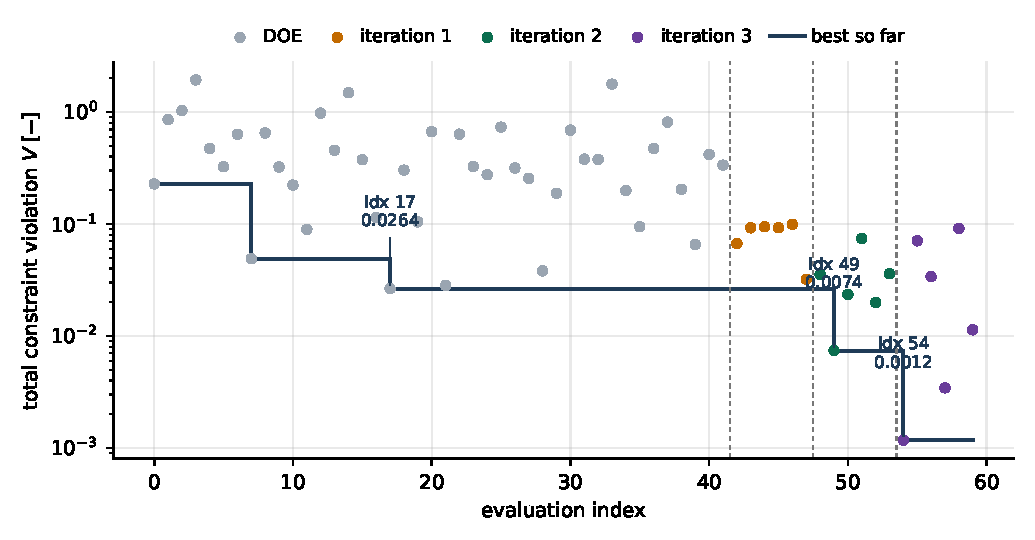
\includegraphics[width=0.95\linewidth]{images/c5_search_trajectory}
  \caption[Campaign 5 search trajectory]{Campaign 5 search trajectory: total normalised constraint violation per evaluation.}
  \label{fig:c5traj}
\end{figure}

All eighteen infill designs sit at the pitch lower bound of
\SI{1.150}{\centi\metre}, extending to six variables the vertex-seeking
behaviour documented for Campaign 4 in
Section~\ref{sec:res-c4-vertex}. Within that plane the three iterations
occupy three distinct regions of the design space
(Fig.~\ref{fig:c5lobes}, design of experiments points in grey):

\begin{enumerate}
  \item iteration 1 proposes 40 rods with gadolinia weight fractions of
        1.8 to 2.4\,wt\%, inner enrichment near the LEU cap at 18.1 to
        18.5\,wt\% and a thin reflector of 2.1 to \SI{5.8}{\centi\metre},
  \item iteration 2 proposes 12 rods with essentially zero gadolinia,
        both enrichments near 7.2\,wt\% and the reflector at its lower
        bound of \SI{2.0}{\centi\metre},
  \item iteration 3 proposes 40 rods with gadolinia weight fractions of
        1.4 to 1.9\,wt\%, inner enrichment near 13.2\,wt\% and the
        reflector at its geometric ceiling of 19.4 to
        \SI{19.5}{\centi\metre}.
\end{enumerate}

One geometric caveat applies to every design at this pitch. The
guide-tube outer radius of \SI{0.6121}{cm} exceeds the half-pitch below
\SI{1.2242}{cm}, and the lattice clips the tube wall at the cell
boundary silently, replacing up to \SI{27}{\percent} of the wall
cross-section by moderator at \SI{1.150}{cm}.

The defect was found while preparing Campaign 8, which fixes the pitch
at \SI{1.26}{cm} (Section~\ref{sec:meth-c8-space}). The vertex-seeking
result stands, because the optimiser was responding to the lattice it
was given. The absolute eigenvalues and peaking values of the
\SI{1.150}{cm} designs nevertheless carry an unquantified bias from the
extra moderator in the guide-tube ring.

\begin{figure}[htbp]
  \centering
  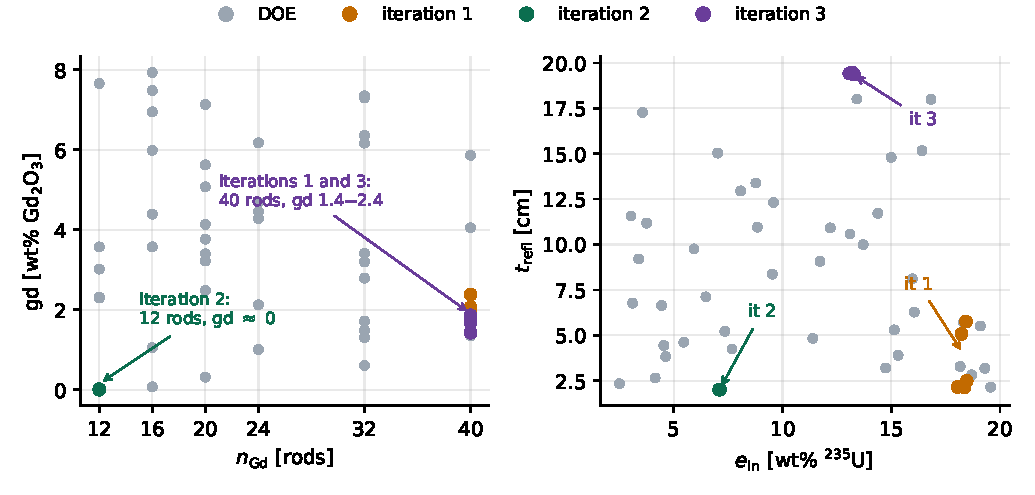
\includegraphics[width=0.95\linewidth]{images/c5_lobes}
  \caption[The two lobes of the Campaign 5 infill]{The two lobes of the Campaign 5 infill. Left, gadolinia weight fraction against rod count. Right, inner enrichment against reflector thickness.}
  \label{fig:c5lobes}
\end{figure}

The 40-rod iterations and the 12-rod iteration are two distinct routes
to the same reactivity screen. The first holds a large fissile inventory
in check with a large absorber inventory. The second carries so little
fissile inventory that almost no absorber is required.

%% AUTHOR: physics interpretation of the two lobes. Why the surrogate
%% found the zero-absorber lobe on its second iteration, what the two
%% routes imply for cycle length (the 12-rod lobe designs cross their
%% reactivity target near 3700 EFPD while the 40-rod lobe designs reach
%% the burnup ceiling), and which lobe is the better engineering basis.

\subsection{Corrected objectives}
\label{sec:res-c5-corrected}

Every cycle length recorded during the campaign is affected by the
depletion restart defect analysed in Section~\ref{sec:restart_defect}.
The salvage procedure of that section recovers the true burnups from the
archived histories without repeating any transport, and every
cycle-length statement in this subsection uses the corrected values. All
beginning-of-life quantities, in particular every peaking factor and
every eigenvalue in this chapter, are unaffected by construction.

The correction changes the population structure. The sixty evaluations
separate into three groups rather than the two reported by the evaluator:

\begin{enumerate}
  \item 18 designs crossed their reactivity target and possess a true,
        finite end of cycle,
  \item 39 designs reached the burnup ceiling, whose corrected physical
        value is \SI{43.0}{\mega\watt\day\per\kilo\gram} rather than the
        labelled \SI{75.0}{\mega\watt\day\per\kilo\gram}, so their
        corrected cycle lengths are lower bounds of \num{4307} Effective
        Full Power Days rather than the recorded \num{7513},
  \item 3 designs never reached criticality against their own
        end-of-cycle target and have no cycle at all. These were
        previously conflated with the ceiling group.
\end{enumerate}

The overstatement factor across the campaign is 1.68 on average, ranging
from 1.23 for early-terminating designs to 1.74 for designs that ran the
full schedule. The 413 discarded dead-step entries carry a mean
reactivity rise of \SI{785}{pcm}, in the range \SIrange{364}{1540}{pcm},
which identifies the chunk-locked period-two oscillation observed in the
recorded histories with the xenon signature of the defect rather than
with a property of the predictor integrator.

Figure~\ref{fig:c5objcorr} places the sixty Campaign 5 evaluations in the
corrected objective plane. Circles are designs that crossed their
reactivity target, plotted at the corrected end of cycle. Triangles are
designs censored at the burnup ceiling, plotted at the corrected ceiling
as lower bounds, and the three never-critical designs have no cycle and
are omitted. The collapse onto the ceiling line is the censoring
distortion of Section~\ref{sec:res-c2}, reproduced at the corrected
ceiling.

\begin{figure}[htbp]
  \centering
  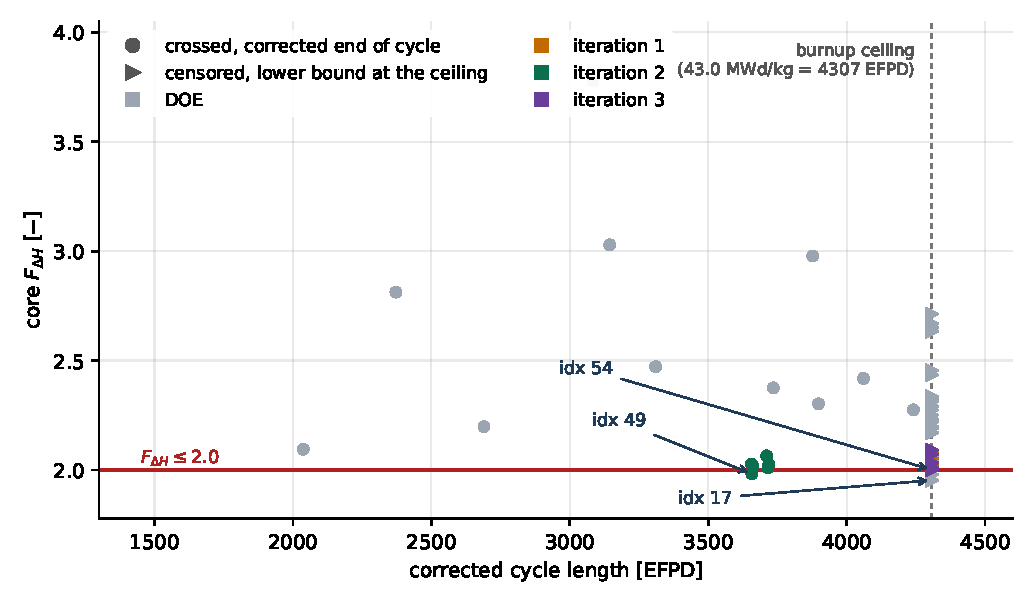
\includegraphics[width=0.95\linewidth]{images/c5_objectives_corrected}
  \caption[Campaign 5 in the corrected objective plane]{Campaign 5 evaluations in the corrected objective plane.}
  \label{fig:c5objcorr}
\end{figure}

Two features of Figure~\ref{fig:c5objcorr} carry the conclusions of the
campaign.

The first is that the ceiling truncates the front. Thirty-nine designs,
including the champion, collapse onto a single cycle-length value, so no
trade-off can be resolved beyond \num{4307} Effective Full Power Days.
The intended ceiling of \SI{75}{\mega\watt\day\per\kilo\gram} was chosen
to sit above every physical end of cycle. The defect silently halved it,
and the corrected value of \SI{43.0}{\mega\watt\day\per\kilo\gram} sits
below the crossing burnup of most of the population. The censoring
lesson of Campaign 2 therefore applies to Campaign 5 in full, through no
choice made in the campaign design.

The second is the identity of the interesting designs, summarised in
Table~\ref{tab:c5-champions}, where feasibility is quoted on both
reactivity bases at the common limit of 1.35. The corrected
non-dominated set consists
of a single design, archive index 17, which pairs the lowest peaking
factor of the entire campaign, $F_{\Delta H} = 1.9534$, with a censored
cycle length of at least \num{4307} Effective Full Power Days. It is a
design-of-experiments point, and the search machinery never treated it
as interesting because its assembly eigenvalue of 1.3764 violates the
as-run reactivity screen. Archive index 49, from the 12-rod lobe, is the
only design in the campaign that combines a sub-limit peaking factor
with a completed, uncensored cycle, at a corrected end of cycle of
\num{3658} Effective Full Power Days, almost exactly ten years at full
power. The campaign champion, index 54, remains the least-infeasible
design under the as-run screens, with the peaking excess of 0.0012 that
the confirmation study of Section~\ref{sec:c5_confirmation} shows to be
statistically indistinguishable from the limit.

\begin{table}[htbp]
  \centering
  \small
  \caption[The three notable designs of Campaign 5]{The three notable designs of Campaign 5 under the corrected objectives. Bold marks a value at a design-space bound.}
  \label{tab:c5-champions}
  \begin{tabularx}{\textwidth}{@{}>{\raggedright\arraybackslash}p{0.27\textwidth}*{3}{>{\centering\arraybackslash}X}@{}}
    \toprule
    Quantity & idx 17, DOE & idx 49, iteration 2 & idx 54, iteration 3 \\
    \midrule
    $e_\mathrm{in}$ / $e_\mathrm{out}$ [wt\%]
      & 16.83 / 14.52 & 7.08 / 7.39 & 13.07 / 15.00 \\
    Gd$_2$O$_3$ content [wt\%]
      & 1.49 & 0.00 & 1.42 \\
    $n_\mathrm{Gd}$ [rods]
      & 32 & \textbf{12} & \textbf{40} \\
    Pitch [cm]
      & 1.154 & \textbf{1.150} & \textbf{1.150} \\
    $t_\mathrm{refl}$ [cm]
      & 17.99 & \textbf{2.00} & 19.41 \\
    Core $F_{\Delta H}$ [--]
      & \textbf{1.9534} & 1.9828 & 2.0012 \\
    Assembly $k_\mathrm{BOL}$ [--]
      & 1.3764 & 1.3574 & 1.3449 \\
    Core $k_\mathrm{eff}$ [--]
      & 1.3060 & 1.2777 & 1.2739 \\
    Corrected cycle length [EFPD]
      & $\geq 4307$ & 3658 & $\geq 4307$ \\
    Feasible, assembly basis
      & no & no & no, by 0.0012 in $F_{\Delta H}$ \\
    Feasible, core basis
      & yes & yes & no, by 0.0012 in $F_{\Delta H}$ \\
    \bottomrule
  \end{tabularx}
\end{table}

The three never-critical designs, archive indices 1, 14 and 22, begin
below their own end-of-cycle targets and therefore fail before the first
depletion step by construction. Their evaluations cost \SI{2.48}{\hour}
in total, 2.3\,\% of the campaign, because the crossing test terminates
them after the beginning-of-life block, at 45 to 57 minutes each against
the campaign mean of 108 minutes. The end-of-cycle test therefore already acts
as an implicit beginning-of-life screen. Making the screen explicit,
\begin{equation}
  g_{k\min} \;=\; k_\mathrm{target}(p,\, t_\mathrm{refl})
  \;-\; k_\mathrm{BOL} \;\leq\; 0 ,
  \label{eq:kmin-selfcons}
\end{equation}

with the terms

\begin{itemize}
  \item $k_\mathrm{BOL}$, the assembly multiplication factor at beginning
        of life, dimensionless,
  \item $k_\mathrm{target}(p,\, t_\mathrm{refl})$, the design-specific
        Route B end-of-cycle target of
        Section~\ref{sec:res-c2}, dimensionless,
\end{itemize}

would reject exactly these three designs before any depletion runs,
recovering the remaining \SI{2.23}{\hour}. Unlike the fixed floor of
1.02, the test contains no arbitrary constant, and it does not reject
archive index 33, a design whose core eigenvalue of 1.011 sits below any
plausible fixed core-level floor yet whose corrected cycle runs to
\num{3084} Effective Full Power Days. The screen is adopted prospectively
for future campaigns and is not applied retrospectively here.

\subsection{Re-scoring the reactivity screen on the core basis}
\label{sec:res-c5-kbasis}

The screening constraint $g_{k\max}$ was applied throughout Campaigns 1
to 5 to the assembly $k_\infty$ of the reflective-boundary depletion
model. Excess reactivity is a budget of the finite core, so the
physically meaningful quantity is the core $k_\mathrm{eff}$, which the
evaluator has recorded for every evaluation since Campaign 4 at no
additional cost. This is the same category distinction that moved the
peaking objective from the assembly to the core in Campaign 4, applied
to the remaining assembly-level constraint. Because both readings exist
in the archives, the question of what the core basis would have changed
is answered by re-scoring, without a single new transport solve.

Figure~\ref{fig:c5kbasis} places every Campaign 4 and Campaign 5
evaluation on the two bases. The points fall in a narrow band displaced
from the identity line by the assembly-to-core gap, and the shaded region
holds the designs that the assembly screen rejects and the core screen
admits at the common limit of 1.35.

\begin{figure}[htbp]
  \centering
  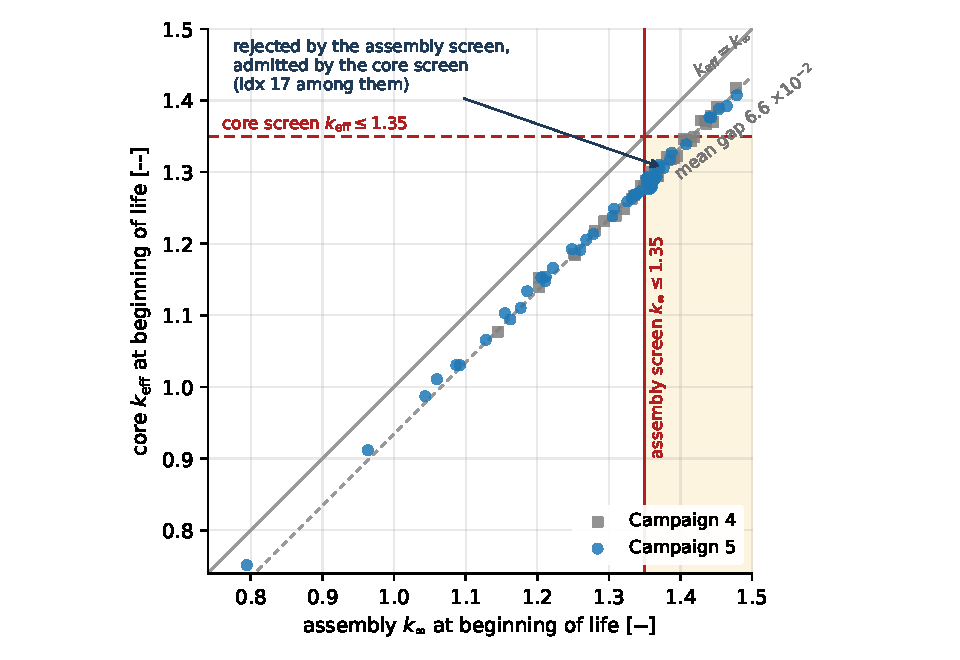
\includegraphics[width=0.82\linewidth]{images/c5_kbasis}
  \caption[The two reactivity bases across Campaigns 4 and 5]{Campaign 4 and Campaign 5 evaluations on the assembly and core reactivity bases.}
  \label{fig:c5kbasis}
\end{figure}

The assembly-to-core gap is large and systematic. Across the Campaign 5
archive it spans \SIrange{4299}{8057}{pcm} with a mean of \SI{6563}{pcm},
and across Campaign 4 it spans \SIrange{5015}{7533}{pcm} with a mean of
\SI{6753}{pcm}. Table~\ref{tab:c5-sweep} sweeps the limit from 1.20 to
1.45 on both bases, with all other constraints held at their campaign
values.

\begin{table}[htbp]
  \centering
  \small
  \caption[Feasible designs under both reactivity bases]{Number of designs satisfying all five screening constraints against the reactivity limit on each basis.}
  \label{tab:c5-sweep}
  \begin{tabular}{c cc cc}
    \toprule
    & \multicolumn{2}{c}{Campaign 4 (54)} &
      \multicolumn{2}{c}{Campaign 5 (60)} \\
    \cmidrule(lr){2-3}\cmidrule(lr){4-5}
    $k$ limit & assembly & core & assembly & core \\
    \midrule
    1.20 & 0 & 0 & 0 & 0 \\
    1.25 & 0 & 0 & 0 & 0 \\
    1.30 & 0 & 6 & 0 & 1 \\
    1.35 & 0 & 7 & 0 & 2 \\
    1.40 & 7 & 7 & 2 & 3 \\
    1.45 & 7 & 7 & 2 & 3 \\
    \bottomrule
  \end{tabular}
\end{table}

Three findings follow.

First, the two formulations that have been under discussion select
identical designs. The core basis at 1.35 admits archive indices 6, 42,
43, 44, 46, 47 and 53 in Campaign 4 and indices 17 and 49 in Campaign 5.
The assembly basis at 1.40 admits exactly the same sets, in both
campaigns. The relaxation to 1.40 and the change of basis are therefore
interchangeable in outcome, and only their justification differs. The
basis change rests on the measured gap and on the physical location of
the excess-reactivity budget, so it is the route adopted here.

Second, the tangency reading of Campaign 4 in
Section~\ref{sec:res-c4-trajectory} does not survive the re-scoring. On
the core basis at 1.35, every one of the 47 infeasible Campaign 4
designs violates the peaking constraint, so $g_{k\max}$ excludes no
design that $g_\mathrm{peak}$ would have admitted. The two constraints
are not tangent. There is a single peaking wall, and the apparent second
wall was the reactivity screen evaluated on a quantity that sits
approximately \SI{6800}{pcm} above the budgeted one. The same holds in
Campaign 5 with a single exception, archive index 16, which passes
peaking at 1.9796 and fails reactivity on both bases. Re-read on the
core basis, the Campaign 4 active learning was more successful than the
as-run accounting showed: its second iteration placed five of six
proposals inside the feasible region, and the third iteration then moved
away from it, because the violation being minimised was computed on the
assembly quantity.

Third, the campaign comparison inverts. Under the as-run screens both
campaigns report zero feasible designs and Campaign 5 reports the
smaller closest approach. Under the core basis Campaign 4 holds seven
feasible designs against two, despite the smaller design space. The
infill pressure toward high absorber inventory, exerted by a reactivity
screen evaluated on the wrong quantity, drove part of the Campaign 5
search into the never-critical region documented above. A constraint
defined on a proxy therefore did not merely mislabel the results. It
steered the search. This is the same failure mode established for the
peaking proxy in Section~\ref{sec:res-corevalidation}, observed a second
time in an independent constraint, which elevates it from an anecdote to
a property of proxy-constrained surrogate optimisation in this design
space.

The limit itself remains a screening value. On the core basis, a
multiplication factor of 1.35 corresponds to approximately
\SI{25900}{pcm} of excess reactivity to be held by the burnable
absorber, the \SI{1000}{ppm} soluble boron of the benchmark basis and
the control rods.

Whether that budget is controllable is a rod-worth question, and
Campaign 7 answers it by measurement. Deriving the ceiling from the
measured worth of all seven banks with a \SI{1000}{pcm} operating
margin gives 1.368 (Section~\ref{sec:res-c7-worth}), so the value of
1.35 used in Campaigns 1 to 6 is the all-bank controllability bound of
this core to within two per cent.

The regulating banks alone hold down considerably less, and from
Campaign 7 the ceiling is replaced as the working constraint by the
measured controllability screen of Section~\ref{sec:meth-ctrl}.

The remaining gap in peaking between this single-batch uniform core and
licensed practice, where a Technical Specification limit of 1.65 on
$F_{\Delta H}$ applies~\cite{robinson_gd10}, is the domain of
multi-batch loading patterns, zoned absorber placement and rod
programmes~\cite{kropaczek_turinsky_1991,aga_firstcore_2021,chasnupp_lpo_2013}.
Those are outside this design space by construction and are the
natural continuation of the work (Section~\ref{sec:concl-future}).

\subsection{High-fidelity confirmation of the Campaign 5 champion}
\label{sec:c5_confirmation}

Campaign 5 returned no design satisfying every as-run screening
constraint in sixty evaluations. The least-infeasible design, archive
index 54, violated only the radial enthalpy-rise constraint, and by an
amount smaller than the run-to-run scatter of the Monte Carlo estimator
that produces it. A separate confirmation study was therefore run to
determine whether that violation is a property of the design or an
artefact of the transport statistics.

The design was re-solved at beginning of life with eight independent
transport seeds at raised fidelity, namely \num{200000} particles per batch
over 260 batches with 80 inactive batches, against the campaign setting of
\num{100000} particles over 170 batches with 60 inactive batches. The
assembly eigenvalue was re-solved with four independent seeds. No depletion
was repeated, because the peaking factor is a beginning-of-life quantity and
the cycle length of this design is set by the burnup ceiling rather than by
the reactivity target. The peaking estimator, the mesh definition and the
Shannon-entropy source-convergence diagnostic were taken unchanged from the campaign
evaluator, so the confirmed quantity is identical in definition to the
optimisation objective.

The sample statistics are formed as

\begin{equation}
\bar{F} = \frac{1}{n}\sum_{i=1}^{n} F_i ,
\qquad
s = \sqrt{\frac{1}{n-1}\sum_{i=1}^{n}\left(F_i - \bar{F}\right)^2 },
\qquad
\mathrm{CI}_{95} = \bar{F} \pm t_{0.975,\,n-1}\,\frac{s}{\sqrt{n}} ,
\end{equation}

with the terms

\begin{itemize}
  \item $F_i$, the radial enthalpy-rise hot channel factor returned by
        transport seed $i$, dimensionless,
  \item $n$, the number of independent seeds, dimensionless,
  \item $\bar{F}$, the sample mean of the peaking factor, dimensionless,
  \item $s$, the sample standard deviation of the peaking factor,
        dimensionless,
  \item $t_{0.975,\,n-1}$, the two-sided Student critical value at the
        \SI{95}{\percent} level with $n-1$ degrees of freedom, dimensionless.
\end{itemize}

The design was declared feasible on a constraint only when the entire
confidence interval clears the limit, which is the conservative test.
Table~\ref{tab:c5_confirmation} gives the result for the champion. The
peaking constraint cannot be separated from its limit.

\begin{table}[htbp]
  \centering
  \caption[Campaign 5 champion confirmed at raised fidelity]{Campaign 5 champion, archive index 54, confirmed at raised fidelity.}
  \label{tab:c5_confirmation}
  \begin{tabular}{lrrrrl}
    \toprule
    Quantity & Mean & $s$ & \multicolumn{2}{c}{\SI{95}{\percent} interval}
             & Verdict \\
    \midrule
    Core $F_{\Delta H}$ ($n=8$)      & 2.00350 & 0.01320 & 1.99246 & 2.01454
                                     & indistinguishable \\
    Assembly $k_{\mathrm{BOL}}$ ($n=4$) & 1.34392 & 0.00030 & 1.34344 & 1.34440
                                     & pass \\
    Core $k_{\mathrm{eff}}$ ($n=8$)  & 1.27424 & --      & --      & --
                                     & not constrained \\
    \bottomrule
  \end{tabular}
\end{table}

The reactivity constraint is settled. The assembly eigenvalue clears the
screening limit of 1.35 by \SI{608}{pcm}, against a seed-to-seed standard
deviation of \SI{30}{pcm}, so the margin exceeds twenty standard errors. The
core eigenvalue of the same design is \SI{6968}{pcm} below the assembly
value, consistent with the range of \SIrange{5012}{7530}{pcm} measured across
the Campaign 4 archive, which confirms that the screening limit is applied to
the more conservative of the two quantities.

The peaking constraint is not settled, and cannot be settled at this
resolution. The mean exceeds the limit of 2.0 by 0.0035, which is
\SI{0.175}{\percent} of the limit and approximately one quarter of one
standard deviation of a single solve. Individual seeds fall on both sides of
the limit, spanning 1.9843 to 2.0217. Reducing the standard error far enough
for the interval to separate from the limit at the observed offset would
require of the order of fifty-five independent seeds, and would establish a
violation of less than two tenths of one percent of a bound that is itself a
relaxed screening value rather than a licensed limit.

Two observations on the estimator follow from the same data set. The
campaign evaluation of this design returned 2.0012 at the lower campaign
fidelity, which falls at the 38th percentile of the eight high-fidelity
seeds, so no fidelity bias is detectable in the optimisation objective. The
measured standard deviation is 1.33 times the value predicted by inverse
square-root scaling of the particle count from the Campaign 3 noise
measurement. This is expected behaviour, because the peaking factor is a
maximum over mesh bins rather than a mean, and extreme-value statistics
converge more slowly than sample means with increasing particle count.

%% AUTHOR: physics interpretation of the gadolinia pin count as the mechanism
%% that moved the constraint boundary without opening an overlap on the
%% as-run basis, read together with the corrected picture of
%% Section~\ref{sec:res-c5-corrected} in which archive indices 17 and 49
%% are feasible on the core basis.

The conclusion for the design space is therefore threefold. Adding the
gadolinia-bearing rod count as a sixth design variable lowered the
minimum total constraint violation from 0.0077 in Campaign 4 to 0.0012
in Campaign 5, so the additional degree of freedom measurably moved the
constraint boundary on the as-run basis. On that basis the best
reachable design lies on the peaking boundary to within the resolution
of the model. On the core reactivity basis of
Section~\ref{sec:res-c5-kbasis}, two designs of this campaign and seven
of the previous one are feasible, and the sole remaining obstacle in the
design space is the peaking wall. Under uniform loading no
distinguishable peaking margin exists beyond it, which motivates the
zoned-loading study as the natural continuation of the work.

% ===================== end of replacement block ======================

\subsection{A defect in the restarted depletion}
\label{sec:restart_defect}

\subsubsection{Depletion in separate blocks}

The depletion solver requires the complete list of burnup steps before the
calculation starts. A single call of the form "burn six steps of
\SI{4}{\mega\watt\day\per\kilo\gram}" runs to the end of that list and
stops.

This requirement conflicts with the definition of the cycle length used in
this work. The end of cycle is the burnup at which the reactivity falls to
the target value, and that burnup is not known before the calculation is
performed, because it is a property of the design being evaluated.

Supplying a fixed list is therefore either insufficient or wasteful. A short
list may end while the reactivity is still far above the target, in which
case the design has not been evaluated at all. A long list continues to burn
fuel after the target has been crossed, at a cost of several minutes of
computing time per unnecessary step. Across the enrichment range explored by
the campaigns, no single fixed list is appropriate for every design.

The evaluator therefore advances the depletion in short blocks and inspects
the reactivity after each one. It continues only while the target has not
been crossed and the burnup ceiling has not been reached. Each block is a
separate call to the depletion solver, and the number of blocks adapts to
the design.

Archive index 7 illustrates the resulting structure. Its depletion consists
of nine blocks:

\begin{enumerate}
  \item the first block advances five steps of 0.5, 1.0, 2.0, 4.0 and
        \SI{6.0}{\mega\watt\day\per\kilo\gram}, reaching
        \SI{13.5}{\mega\watt\day\per\kilo\gram},
  \item the second through eighth blocks each advance two steps of
        \SI{4.0}{\mega\watt\day\per\kilo\gram},
  \item the ninth block advances \SI{4.0}{} and then
        \SI{1.5}{\mega\watt\day\per\kilo\gram}, stopping at the burnup
        ceiling rather than at a reactivity crossing.
\end{enumerate}

\subsubsection{How one block continues from the previous one}

Consecutive blocks are not independent calculations. Each block must begin
with the fuel in exactly the state the previous block left it, including the
depleted uranium content, the accumulated plutonium and the fission product
inventory.

The continuation is performed through the results file. A block writes its
final state to disk, and the next block reads that file and passes it to a
new depletion operator as the previous state. This operation is referred to
here as a restart. The nine blocks of archive index 7 therefore involve
eight restarts.

A results file is expected to carry two distinct kinds of information:

\begin{enumerate}
  \item the material composition, which specifies how much of each nuclide
        is present,
  \item the reaction rates, which specify how rapidly each nuclide is being
        transmuted at the current flux level.
\end{enumerate}

The composition tells the solver where the fuel is. The reaction rates tell
it how fast the fuel is changing. A restart requires both, because the first
step after a restart is advanced using the reaction rates carried over from
the end of the previous block.

\subsubsection{Origin of the restart defect}

Version 0.15.3 of the depletion solver introduced an option controlling
whether reaction rates are written to the results file, and set its default
to false in order to reduce file size. The evaluator did not set this
option, so the results files written by every block contained the material
composition but no reaction rates.

A results object reconstructed from such a file carries an empty reaction
rate structure, because the reconstruction relies on metadata that is absent
from the file. The restart routine reads that structure and passes it to the
solver without verifying that it is populated.

The consequence is that the first step of every restarted block was advanced
with all transmutation channels set to zero. The material composition
evolved by radioactive decay alone. No fission occurred, no fission products
were produced, and no burnup was accumulated. The burnup label maintained by
the evaluator was nevertheless advanced by the full step.

The failure was silent. The calculation completed without error, and every
value it returned was of a plausible magnitude.

\subsubsection{The signature in the recorded history}

Figure~\ref{fig:restart_defect}(a) shows the depletion history of archive
index 7 as the evaluator recorded it. The points separate into two branches
approximately \SI{950}{pcm} apart.

The upper branch consists of the first point of every restarted block. These
are the steps in which the fuel did not burn. Physical time advanced
nonetheless, so xenon-135 decayed without being replaced by fission and the
reactivity rose. The measured rises are 1040, 1029, 963, 1232, 926, 1019,
732 and \SI{670}{pcm}, with a mean of \SI{951}{pcm} and a standard deviation
of \SI{179}{pcm}. A positive reactivity excursion of this magnitude,
occurring exclusively at block boundaries and nowhere else, is
characteristic of xenon removal and is not consistent with any depletion
process.

The lower branch consists of the second point of every block. These points
are physically correct. Their burnup labels, however, have advanced twice as
fast as the fuel. Figure~\ref{fig:restart_defect}(b) plots the same
measured reactivities against the burnup the fuel actually reached,
together with an independent control calculation performed as a single
uninterrupted block, and the corrected trajectory agrees with the control
calculation.

\begin{figure}[htbp]
  \centering
  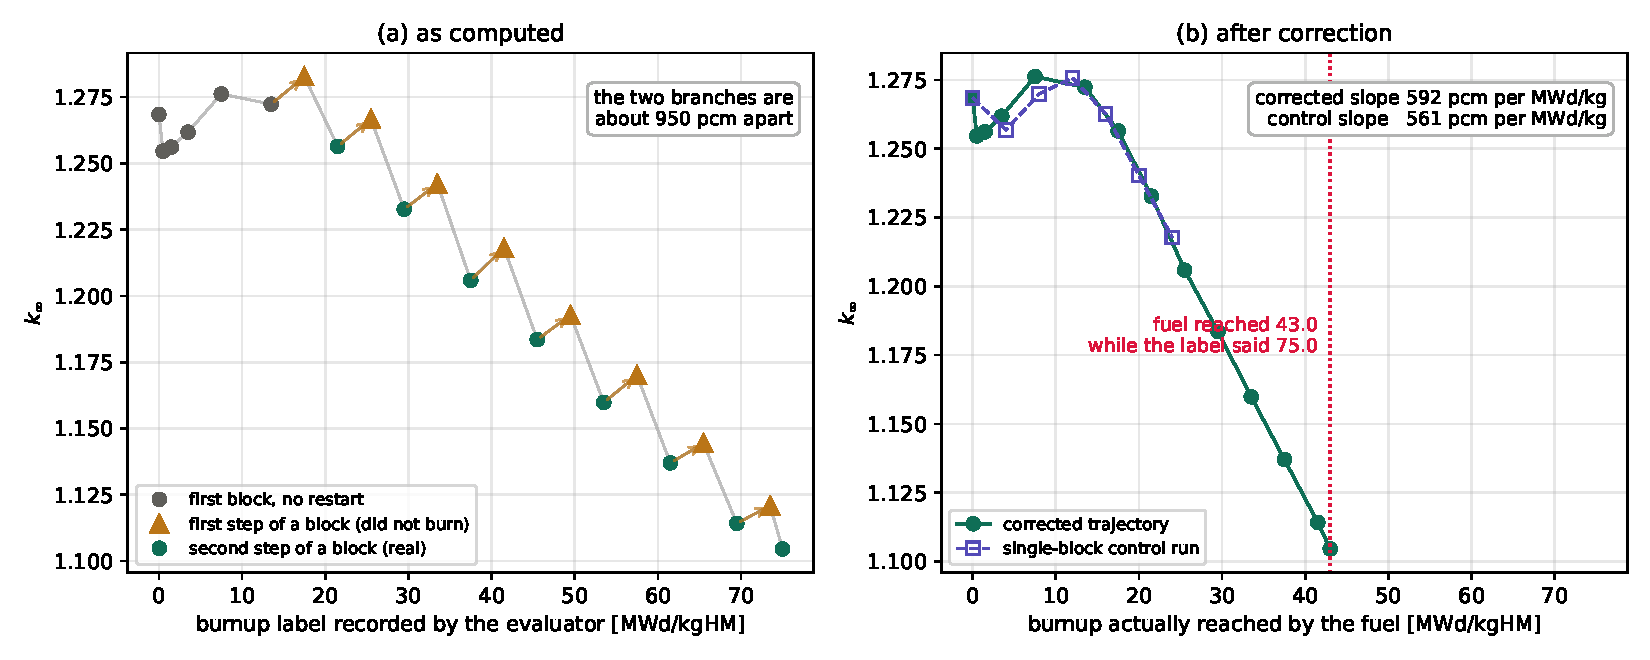
\includegraphics[width=\textwidth]{images/fig_restart_defect.pdf}
  \caption[Depletion history of archive index 7]{Depletion history of archive index 7. (a)~As recorded. (b)~Against the burnup actually reached, with the control calculation.}
  \label{fig:restart_defect}
\end{figure}

\subsubsection{The controlled experiment}

The mechanism was confirmed by depleting archive index 7 twice through the
same model and the same random seed, with the only difference being the
block structure:

\begin{enumerate}
  \item arm A, a single uninterrupted block of six steps of
        \SI{4}{\mega\watt\day\per\kilo\gram},
  \item arm B, three blocks of two steps covering the identical burnup
        points.
\end{enumerate}

Because the model and the seed are shared, the two arms compute the same
quantity at every point and must agree to within the statistical scatter of
the transport solution. Table~\ref{tab:restart_experiment} compares the
two arms.

\begin{table}[htbp]
  \centering
  \caption{Reactivity of archive index 7 computed with and without block restarts.}
  \label{tab:restart_experiment}
  \begin{tabular}{rrrrl}
    \toprule
    Burnup label & Arm A & Arm B & Difference & Position \\
    $[$\si{\mega\watt\day\per\kilo\gram}$]$ & $k_\infty$ & $k_\infty$
      & [\si{pcm}] & \\
    \midrule
     0 & 1.26846 & 1.26846 &    0 & start \\
     4 & 1.25680 & 1.25736 &  +56 & before any restart \\
     8 & 1.26988 & 1.27067 &  +79 & first restart point \\
    12 & 1.27568 & 1.28094 & +526 & first step after a restart \\
    16 & 1.26267 & 1.27436 & +1169 & second restart point \\
    20 & 1.24028 & 1.28461 & +4433 & first step after a restart \\
    24 & 1.21775 & 1.26382 & +4607 & final point \\
    \bottomrule
  \end{tabular}
\end{table}

Table~\ref{tab:restart_experiment} supports the mechanism in two independent
ways.

The first is the location of the divergence. At 0, 4 and
\SI{8}{\mega\watt\day\per\kilo\gram} the two arms differ by 0, 56 and
\SI{79}{pcm}, which is the ordinary scatter of the transport solution at the
campaign settings. Divergence begins at exactly
\SI{12}{\mega\watt\day\per\kilo\gram}, the first point computed after the
first restart, and grows monotonically thereafter.

The second is the size of the divergence. If each restart consumes one step
without burning the fuel, then the arm B point labelled 16 is the true state
at 12, and the point labelled 24 is the true state at 16. The measured
values are 1.27436 against 1.27568, a difference of \SI{-132}{pcm}, and
1.26382 against 1.26267, a difference of \SI{115}{pcm}. Both lie inside the
statistical scatter. The chunked calculation is therefore not incorrect in
an unstructured way. It is behind by exactly one step per restart.

\subsubsection{Correcting the recorded histories}

For blocks of two steps, the burnup label advances twice as fast as the
fuel. The relation between the two is

\begin{equation}
B_{\mathrm{true}} = B_{0} + \frac{B_{\mathrm{label}} - B_{0}}{2} ,
\label{eq:true_burnup}
\end{equation}

with the terms

\begin{itemize}
  \item $B_{\mathrm{label}}$, the cumulative burnup recorded by the
        evaluator, in \si{\mega\watt\day\per\kilo\gram} of heavy metal,
  \item $B_{\mathrm{true}}$, the burnup physically reached by the fuel, in
        the same units,
  \item $B_{0}$, the burnup at the end of the first block, which contains no
        restart and is therefore unaffected, equal to
        \SI{13.5}{\mega\watt\day\per\kilo\gram} for the schedule used here.
\end{itemize}

Figure~\ref{fig:restart_defect}(b) applies this correction. The points of
the upper branch are discarded, because they duplicate the state preceding
them, and the remaining points are relabelled. The two branches collapse
onto a single smooth trajectory.

Two quantitative checks confirm the correction. The corrected trajectory
falls at \SI{592}{pcm} per unit of burnup, against \SI{561}{pcm} measured in
the independent single-block control calculation, an agreement of
\SI{5}{\percent}. The control calculation itself is plotted in
Figure~\ref{fig:restart_defect}(b) and lies on the corrected trajectory.

Applying Equation~\ref{eq:true_burnup}, the reported ceiling of
\SI{75.0}{\mega\watt\day\per\kilo\gram} for archive index 7 corresponds to a
physical burnup of \SI{43.0}{\mega\watt\day\per\kilo\gram}. The reported
cycle length of \num{7513} Effective Full Power Days corresponds to
\num{4307}, an overstatement by a factor of 1.74.

\subsubsection{Scope of the affected results}

The defect affects only quantities that depend on depletion beyond the first
block. The following results are unaffected and require no revision:

\begin{itemize}
  \item all beginning of life quantities, including every core radial
        peaking factor and every assembly eigenvalue at zero burnup,
  \item the transfer test and the multiplier optimisation of the
        zoned-loading study, whose multipliers now enter the
        methodology in Section~\ref{sec:meth-zoning} and which are
        computed at beginning of life. Its Stage 3 confirmation does
        deplete, but both runs completed after the correction was
        committed, as recorded in Section~\ref{sec:meth-zoning-study},
  \item the feasibility assessment against the peaking constraint and
        against the beginning of life reactivity constraint.
\end{itemize}

The following results require correction:

\begin{itemize}
  \item every cycle length obtained from a trajectory that crossed the
        reactivity target, which is overstated,
  \item every burnup reported at the ceiling, which is overstated by
        Equation~\ref{eq:true_burnup},
  \item every reactivity slope derived from the affected histories, which is
        understated by approximately a factor of two.
\end{itemize}

The depletions do not need to be repeated. The physical states already
computed are correct and only their burnup labels are wrong, so the archived
histories can be corrected by discarding the first entry of each block and
applying Equation~\ref{eq:true_burnup}.

The solver version question is closed. The pinned environments of
Section~\ref{sec:meth-diagnostics} carry OpenMC 0.15.3 on both hosts
for every campaign, so Campaigns 1 to 5 all executed under the
affected default and the correction applies to the whole archive.
Campaign 6 is the first campaign to run entirely under the corrected
configuration, and its checkpoint metadata records the setting.

\subsubsection{Correction applied to the evaluator}

The evaluator was modified to request that reaction rates be written to the
results file. A verification was added that raises an error if a results
object about to be used for a restart carries an empty reaction rate
structure. The verification is deliberately fatal rather than advisory,
because the condition it detects produces physically plausible output and
would otherwise remain undetected.

The controlled experiment of Table~\ref{tab:restart_experiment} was repeated
after the correction as an acceptance test, with the criterion that the two
arms agree at every point to within the statistical scatter of the transport
solution.

%% AUTHOR: state the physical interpretation of the corrected cycle lengths
%% and their relation to the fuel burnup limits discussed in the constraint
%% sourcing section, noting that the corrected ceiling burnup of
%% 43.0 MWd/kgHM lies below both the 62 GWd/t rod average and the
%% 55 GWd/t assembly average values.

\subsubsection{Methodological observation}

This is the fourth defect in this work identified by subjecting the model to
a condition its author had not anticipated, following an inconsistency in a
geometric padding constant, a failure of the optimiser when no feasible
design exists, and an incorrect reading of the output of a restarted
depletion. In each case the calculation completed without error and returned
values of plausible magnitude.

The common feature is that each defect was exposed by a deliberate
consistency test rather than by inspection of the source code. The present
case is the strongest instance, because the defect arises in a widely used
external code operating in its default configuration, and the test that
revealed it consists of performing the same calculation in two ways that
must agree.

%% AUTHOR: decide whether to report this defect to the maintainers of the
%% depletion solver, and if so, cite the report here.

\section{Campaign 6: the corrected basis and the acquisition programme}
\label{sec:res-c6}
\label{sec:res-c6-blocks}

Campaign 6 applies the three corrections established by the Campaign 5
analyses, namely the core-basis reactivity window, the evaluator-level
radial zoning and the raised depletion horizon, and then uses the
campaign itself as a controlled test bench for the acquisition
function. The campaign comprises \num{114} evaluations in five blocks.
The design of experiments is followed by four infill blocks, and each
infill block changes exactly one element of the acquisition of
Section~\ref{sec:meth-acq}, so every behavioural change is
attributable. Table~\ref{tab:c6-blocks} gives the block structure, with
the hypervolume taken as the archive value against the frozen reference
point after the last iteration of each block.

\begin{table}[htbp]
  \centering
  \small
  \caption{Campaign 6 block structure.}
  \label{tab:c6-blocks}
  \begin{tabularx}{\textwidth}{@{}lcc>{\raggedright\arraybackslash}Xc@{}}
    \toprule
    Block & Evaluations & Feasible & Acquisition state & Hypervolume \\
    \midrule
    1, DOE & 42 & 28 & none, Latin hypercube          & 1288.09 \\
    2      & 18 & 13 & bare uncertainty ranking       & 1288.09 \\
    3      &  6 &  1 & + batch diversity              & 1288.09 \\
    4      & 18 & 17 & + feasibility margin           & 1580.05 \\
    5      & 30 & 29 & unchanged, convergence check   & 1601.51 \\
    \bottomrule
  \end{tabularx}
\end{table}

\subsection{Design of experiments}
\label{sec:res-c6-doe}

The 42-point Latin hypercube returned 28 feasible designs, against
zero in the Campaign 5 design of experiments of identical size. Every
rejection is fully explained by the active constraints.

\begin{itemize}
  \item Ten designs exceed the peaking limit of 2.0.

  \item Five designs fall below the reactivity floor of 1.02 on the
        core basis, including one that never reaches criticality at
        all, with $k_\mathrm{eff}^\mathrm{core} = 0.817$.

  \item Two designs exceed the reactivity ceiling of 1.35.

  \item No design violates the zoned enrichment cap, which the search
        box of Equation~\eqref{eq:leu-box} guarantees by construction.

  \item Four designs violate two constraints simultaneously, which
        reconciles the counts with the 14 rejections.
\end{itemize}

The floor rejections are the first practical consequence of the basis
change. On the assembly basis of Campaigns 1 to 5 the floor of 1.02
never acted. On the core basis it rejects genuinely subcritical cores,
which answers the standing question of whether that bound carries any
physical content.

The Pareto front of the design of experiments holds two designs, at
\num{9445} effective full power days with $F_{\Delta H} = 1.6554$ and
at \num{9035} with $F_{\Delta H} = 1.5741$. Exactly one design
censored at the ceiling, at \num{10016.7} effective full power days
and \SI{100.0}{\mega\watt\day\per\kilo\gram}, and it is infeasible on
the reactivity ceiling in any case.

The frozen hypervolume reference point is constructed from this
two-design front by the nadir-plus-offset rule, at \num{6776}
effective full power days and 2.0692 in peaking. The consequences of
freezing the reference on so small a front are examined in
Section~\ref{sec:res-c6-margin}.

\subsection{Blocks 2 and 3: two acquisition defects, measured}
\label{sec:res-c6-defects}

\subsubsection{Block 2: batch collapse}

Block 2 ran the bare uncertainty ranking of
Equation~\eqref{eq:acq-score} for three iterations of six evaluations.
The batches collapsed. Within each iteration the six selected designs
are near copies of one design, and the eighteen evaluations bought
three distinct design points. The second iteration is representative.
Table~\ref{tab:c6-b2-collapse} lists its six designs. The inner
enrichment spans 0.03~wt\%, the pitch is identical to three decimals in
five of the six, and the reflector spans \SI{0.1}{\centi\metre}.

\begin{table}[htbp]
  \centering
  \caption{Campaign 6, block 2, iteration 2: the six infill designs.}
  \label{tab:c6-b2-collapse}
  \begin{tabular}{cccccc}
    \toprule
    Index & $e_\mathrm{in}$ (wt\%) & $e_\mathrm{out}$ (wt\%) &
    $p$ (cm) & $t_\mathrm{refl}$ (cm) & EFPD \\
    \midrule
    48 & 4.42 & 3.77 & 1.380 & 5.4 & 2011 \\
    49 & 4.44 & 3.77 & 1.380 & 5.4 & 2002 \\
    50 & 4.45 & 3.83 & 1.380 & 5.4 & 2047 \\
    51 & 4.45 & 3.82 & 1.380 & 5.4 & 2053 \\
    52 & 4.43 & 3.77 & 1.380 & 5.4 & 2009 \\
    53 & 4.42 & 3.75 & 1.381 & 5.3 & 1985 \\
    \bottomrule
  \end{tabular}
\end{table}

Two mechanisms combine. The top of a smooth uncertainty field is a
neighbourhood, so the six highest-scoring candidates are adjacent, and
the duplicate test then in force compared raw design vectors at a
tolerance of $10^{-6}$, which only exact numerical copies can fail.
Designs 0.01~wt\% apart passed it four orders of magnitude clear.

The hypervolume did not move in any of the three iterations. The front
nevertheless grew from two designs to six, entirely at the short-cycle
end, including the first design of the whole programme to clear the
1.50 licensing-style screen, at $F_{\Delta H} = 1.4041$ and \num{1054}
effective full power days. The frozen reference point sits at
\num{6776} effective full power days, so every one of these additions
contributes exactly zero to the reported metric. Recomputed against a
full-range reference the archive hypervolume rises from \num{4643} to
\num{4876} across the block, which quantifies what the frozen metric
hides.

\subsubsection{Block 3: constraint blindness}

Block 3 added the batch-diversity separation of
Equation~\eqref{eq:batch-div} at $\delta_\mathrm{min} = 0.10$ and
nothing else. The separation worked as designed. The six picks are
distinct, the pitch spans its full box and the reflector spans
\num{2.0} to \SI{19.5}{\centi\metre}, and no relaxation was required.

With the collapse removed, the next defect became visible. Five of the
six designs returned infeasible on the reactivity ceiling.
Table~\ref{tab:c6-b3-fail} lists the outcomes, with the margin taken as
the excess of $k_\mathrm{eff}^\mathrm{core}$ over the ceiling of 1.35.

\begin{table}[htbp]
  \centering
  \caption{Campaign 6, block 3: infill outcomes.}
  \label{tab:c6-b3-fail}
  \begin{tabular}{ccccc}
    \toprule
    Index & EFPD & $F_{\Delta H}$ & $k_\mathrm{eff}^\mathrm{core}$ &
    Margin (pcm) \\
    \midrule
    60 & 3776 & 1.6430 & 1.29510 & feasible \\
    61 & 8167 & 1.7288 & 1.36533 & $+1533$ \\
    62 & 8395 & 1.7380 & 1.37574 & $+2574$ \\
    63 & 9023 & 1.7324 & 1.39692 & $+4692$ \\
    64 & 9806 & 1.8328 & 1.42680 & $+7680$ \\
    65 & 9728 & 1.7408 & 1.42745 & $+7745$ \\
    \bottomrule
  \end{tabular}
\end{table}

The mechanism is visible in one column of the archive. The gadolinia
content of all six designs is exactly zero. The objective surrogate had
learned that the absorber costs cycle length and drove it out, the
enrichments rose toward the box ceiling, and nothing remained to hold
beginning-of-life reactivity inside the window. The constraint
surrogate predicted feasibility for all five failures even though the
archive already contained a design at
$k_\mathrm{eff}^\mathrm{core} = 1.402$ in that corner. The
Gaussian-process mean is optimistic where the data is thin, and the
bare acquisition never asked it for margin.

\subsection{Blocks 4 and 5: the margin and the convergence}
\label{sec:res-c6-margin}

Block 4 added the feasibility margin of
Equation~\eqref{eq:feas-margin} at $\kappa = 1.5$ and nothing else.
The effect was immediate on all three indicators.

\begin{enumerate}
  \item Seventeen of eighteen designs returned feasible. The single
        failure exceeds the ceiling by \num{151}\,pcm, against
        \num{1533} to \num{7745} in block 3. The search moved from
        wandering deep into the forbidden region to riding the
        constraint boundary.

  \item The gadolinia returned, at 1.57 to 3.30~wt\% in the first
        iteration, then probing the upper bound at 7.92 to 8.00, then
        the dilute alternative at 0.64 to 0.70. The optimiser was
        mapping the absorber trade rather than deleting it.

  \item The hypervolume moved for the first time in the campaign, from
        1288.09 to 1525.01, then 1548.33, then 1580.05, gains of
        18.39, 1.53 and 2.05 per cent.
\end{enumerate}

The margin filter also behaved as a learning indicator. The number of
margin-feasible candidates out of 300 moved from 257 to 168 to 202
across the three iterations, tightening when the first batch taught
the constraint surrogate about the high-enrichment corner and
loosening as further evidence accumulated.

Block 5 changed nothing in the acquisition and ran five iterations at
$\delta_\mathrm{min} = 0.14$ as a convergence check. The hypervolume
gains were 0.60, 0.49, 0.21, 0.05 and 0.02 per cent, five consecutive
iterations below the one per cent threshold. The single censored
design of the archive is infeasible and off the front, so both
conditions of the stopping rule of Section~\ref{sec:meth-loop} are
met and the campaign terminates at \num{114} evaluations.

Two independent signals corroborate the termination.

\begin{enumerate}
  \item The diversity relaxation cascade deepened monotonically. The
        first block 5 iteration already needed relaxation to 0.0175 to
        fill its batch, and the fifth found not a single candidate
        even at that value and completed below 0.009. The surrogate
        front no longer contains materially new designs.

  \item The margin-feasible count rose monotonically from 160 to 266
        of 300, so the constraint surrogate had stopped revising its
        map of the feasible region.
\end{enumerate}

The same stopping rule had already fired once before, falsely. After
block 3 the campaign showed three consecutive iterations at exactly
zero gain while the acquisition was demonstrably selecting duplicates
and then constraint violations. Read literally, the rule declared a
broken search converged. The two firings differ in every indicator
except the hypervolume itself, which is the experimental basis for
treating the rule as necessary and not sufficient, and for the health
indicators added to Section~\ref{sec:meth-loop}.

The two settings established across blocks 4 and 5, the feasibility
margin of 1.5 standard deviations and the minimum separation of 0.14,
were not passed to the Campaign 7 launcher. Two of that campaign's
three infill blocks collapsed in exactly the way documented for blocks
2 and 3 above (Section~\ref{sec:res-c7-blocks}). Both settings are
stated explicitly on the command line from Campaign 8, and a flat
hypervolume is read as a stopping signal only when the acquisition is
known to be functioning.

Figure~\ref{fig:c6-convergence} shows the archive hypervolume after every
evaluation, under the frozen in-campaign reference in the top panel and
under a full-range reference in the bottom panel, with the five blocks
shaded. The frozen metric is flat through blocks 2 and 3 while the
full-range metric shows their genuine short-cycle contribution, and the
first improvement visible to the frozen metric coincides exactly with the
feasibility margin of block 4.

\begin{figure}[htbp]
  \centering
  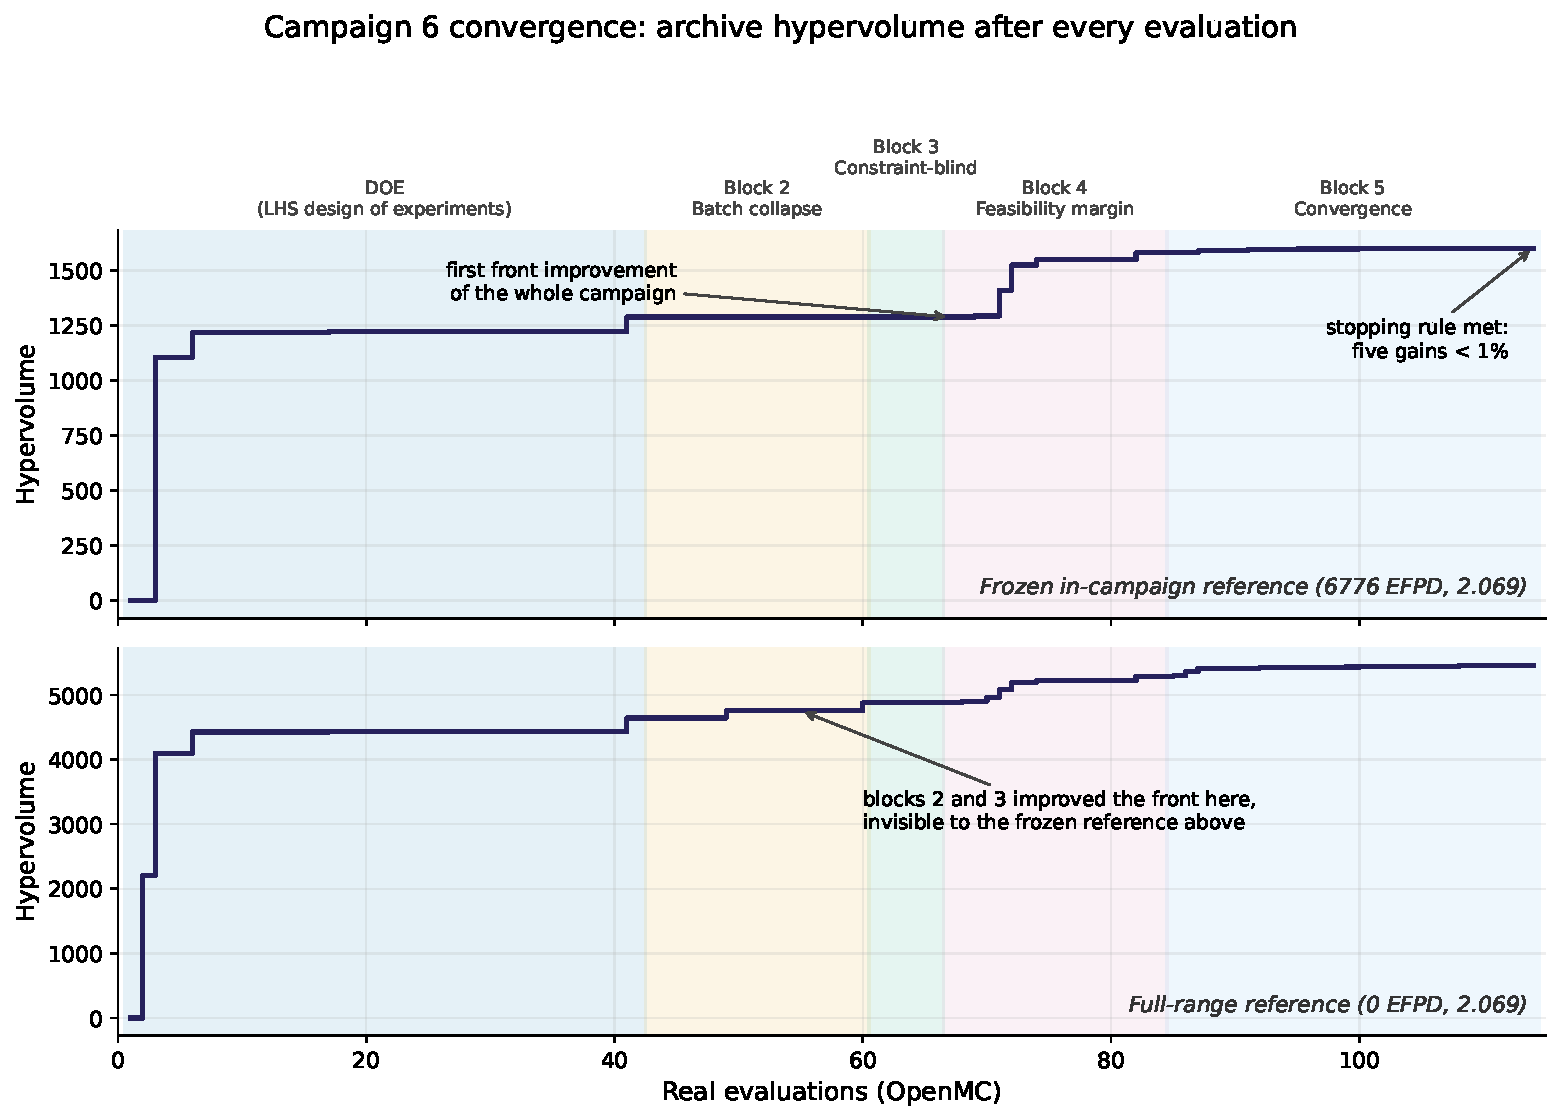
\includegraphics[width=\linewidth]{images/c6_extra_convergence}
  \caption{Campaign 6 convergence: archive hypervolume under the frozen and the full-range reference points.}
  \label{fig:c6-convergence}
\end{figure}

\subsection{The resolved front}
\label{sec:res-c6-front}

Figure~\ref{fig:c6-front} shows the objective space after \num{114}
evaluations. Feasible designs are coloured by block, infeasible designs
are crosses in the colour of their block, and the step line is the
Pareto front of the feasible set. The frozen hypervolume reference point
and the licensing-style screens at 1.65 and 1.50 are drawn for context.

\begin{figure}[htbp]
  \centering
  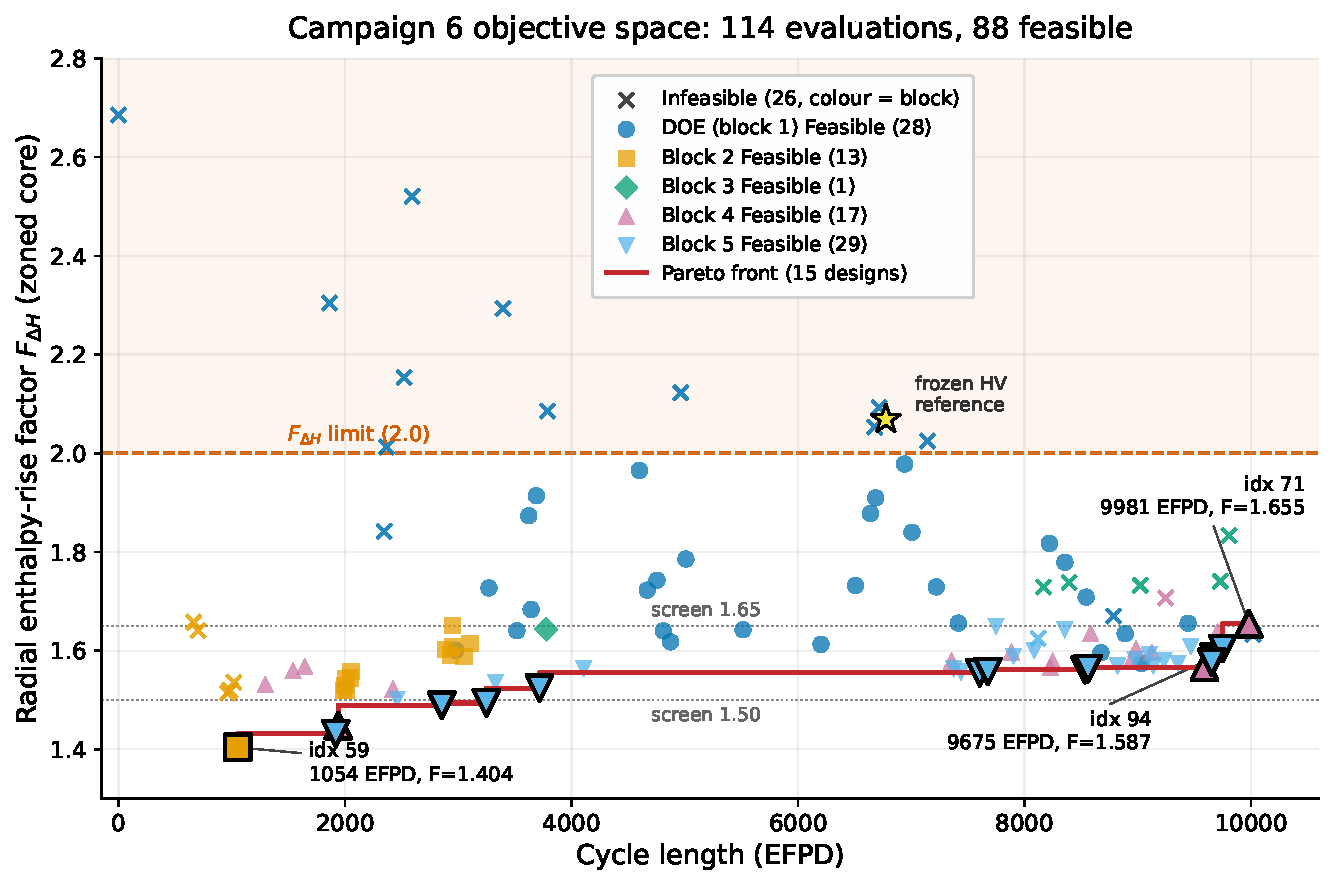
\includegraphics[width=\linewidth]{images/c6_pareto_front_114}
  \caption{Campaign 6 objective space after \num{114} evaluations.}
  \label{fig:c6-front}
\end{figure}

The final front holds fifteen designs and spans the full trade, from
\num{1054} effective full power days at $F_{\Delta H} = 1.4041$ to
\num{9981} at 1.6547 (Table~\ref{tab:c6-front}). In the table the
peaking factor is the zoned-core beginning-of-life value, the eigenvalue
is on the core basis and the burnup is the end-of-cycle value. The pin
count is omitted because every front design carries 40
gadolinium-bearing pins, and the cycle lengths are two-dimensional
exploration-tier values in the sense of Sections~\ref{sec:meth-fidelity}
and~\ref{sec:meth-lax}.

\begin{table}[htbp]
  \centering
  \small
  \caption{The Campaign 6 Pareto front.}
  \label{tab:c6-front}
  \begin{tabular}{cccccccccc}
    \toprule
    Index & EFPD & $F_{\Delta H}$ & $k_\mathrm{eff}^\mathrm{core}$ &
    $B_\mathrm{EOC}$ & $e_\mathrm{in}$ & $e_\mathrm{out}$ &
    gd & $p$ & $t_\mathrm{refl}$ \\
     & (d) & & & (MWd/kg) & (wt\%) & (wt\%) & (wt\%) & (cm) & (cm) \\
    \midrule
     71 & 9981 & 1.6547 & 1.27234 & 99.6 & 15.05 & 15.23 & 3.30 & 1.388 &  2.8 \\
     99 & 9749 & 1.6042 & 1.34126 & 97.3 & 14.86 & 14.49 & 0.51 & 1.338 &  2.1 \\
     94 & 9675 & 1.5866 & 1.33076 & 96.6 & 14.76 & 14.53 & 0.66 & 1.327 &  7.8 \\
    105 & 9653 & 1.5764 & 1.34626 & 96.4 & 14.85 & 14.43 & 0.44 & 1.318 &  9.2 \\
     81 & 9588 & 1.5666 & 1.33150 & 95.7 & 14.87 & 14.18 & 0.66 & 1.354 &  7.0 \\
    103 & 8561 & 1.5635 & 1.33901 & 85.5 & 14.49 & 14.16 & 0.23 & 1.214 & 15.5 \\
     90 & 8535 & 1.5612 & 1.34353 & 85.2 & 14.65 & 14.09 & 0.19 & 1.214 & 13.0 \\
    112 & 7677 & 1.5577 & 1.31137 & 76.6 & 14.43 & 13.83 & 0.23 & 1.154 & 19.2 \\
     86 & 7605 & 1.5550 & 1.27859 & 75.9 & 14.44 & 13.92 & 0.63 & 1.150 & 19.4 \\
     91 & 3717 & 1.5241 & 1.28575 & 37.1 &  5.73 &  6.04 & 0.00 & 1.430 &  2.3 \\
     85 & 3248 & 1.4938 & 1.26117 & 32.4 &  5.05 &  5.49 & 0.00 & 1.396 &  4.2 \\
    110 & 2855 & 1.4894 & 1.13427 & 28.5 &  4.84 &  4.98 & 0.12 & 1.430 &  2.1 \\
     69 & 1941 & 1.4480 & 1.12128 & 19.4 &  4.03 &  3.72 & 0.04 & 1.302 &  9.7 \\
    107 & 1919 & 1.4317 & 1.17329 & 19.2 &  3.99 &  3.84 & 0.00 & 1.430 &  2.0 \\
     59 & 1054 & 1.4041 & 1.07087 & 10.5 &  2.99 &  2.99 & 0.01 & 1.390 &  4.8 \\
    \bottomrule
  \end{tabular}
\end{table}

Design 81 dominates the design-of-experiments champion on both
objectives simultaneously, at \num{9588} against \num{9035} effective
full power days and 1.5666 against 1.5741 in peaking, and clears the
1.60 licensing-style screen at
$k_\mathrm{eff}^\mathrm{core} = 1.332$. Designs 94, 105 and 99 extend
the cycle further at a graded peaking cost, and design 71 gives the
longest cycle but sits at \SI{99.6}{\mega\watt\day\per\kilo\gram},
four tenths of a unit from the depletion horizon, so its cycle length
is effectively bounded by the horizon and is reported with that
caveat.

Eleven of the fifteen front designs come from block 5, three from
block 4 and one from block 2. Not a single design-of-experiments point
survives on the final front. The repaired acquisition displaced both
of the campaign's own starting champions.

A geometric defect found after this campaign qualifies four front
designs. Below a pitch of \SI{1.2242}{cm}, twice the guide-tube outer
radius, the lattice clips the guide-tube wall silently and replaces
part of it by moderator (Section~\ref{sec:res-c7-limits}). Designs
103 and 90 at \SI{1.214}{cm}, 112 at \SI{1.154}{cm} and 86 at
\SI{1.150}{cm} are in the affected band, and their peaking and
eigenvalue carry an unquantified bias. The long-cycle champions 81, 94,
105, 99 and 71 sit between \num{1.318} and \SI{1.388}{cm} and are
unaffected. Campaign 8 removes the defect prospectively by fixing the
pitch at \SI{1.26}{cm}.

Figure~\ref{fig:c6-parallel} shows the fifteen front designs across the
six design variables, each variable normalised to its own search box and
each line coloured by cycle length, over the 88 feasible designs in
grey.

\begin{figure}[htbp]
  \centering
  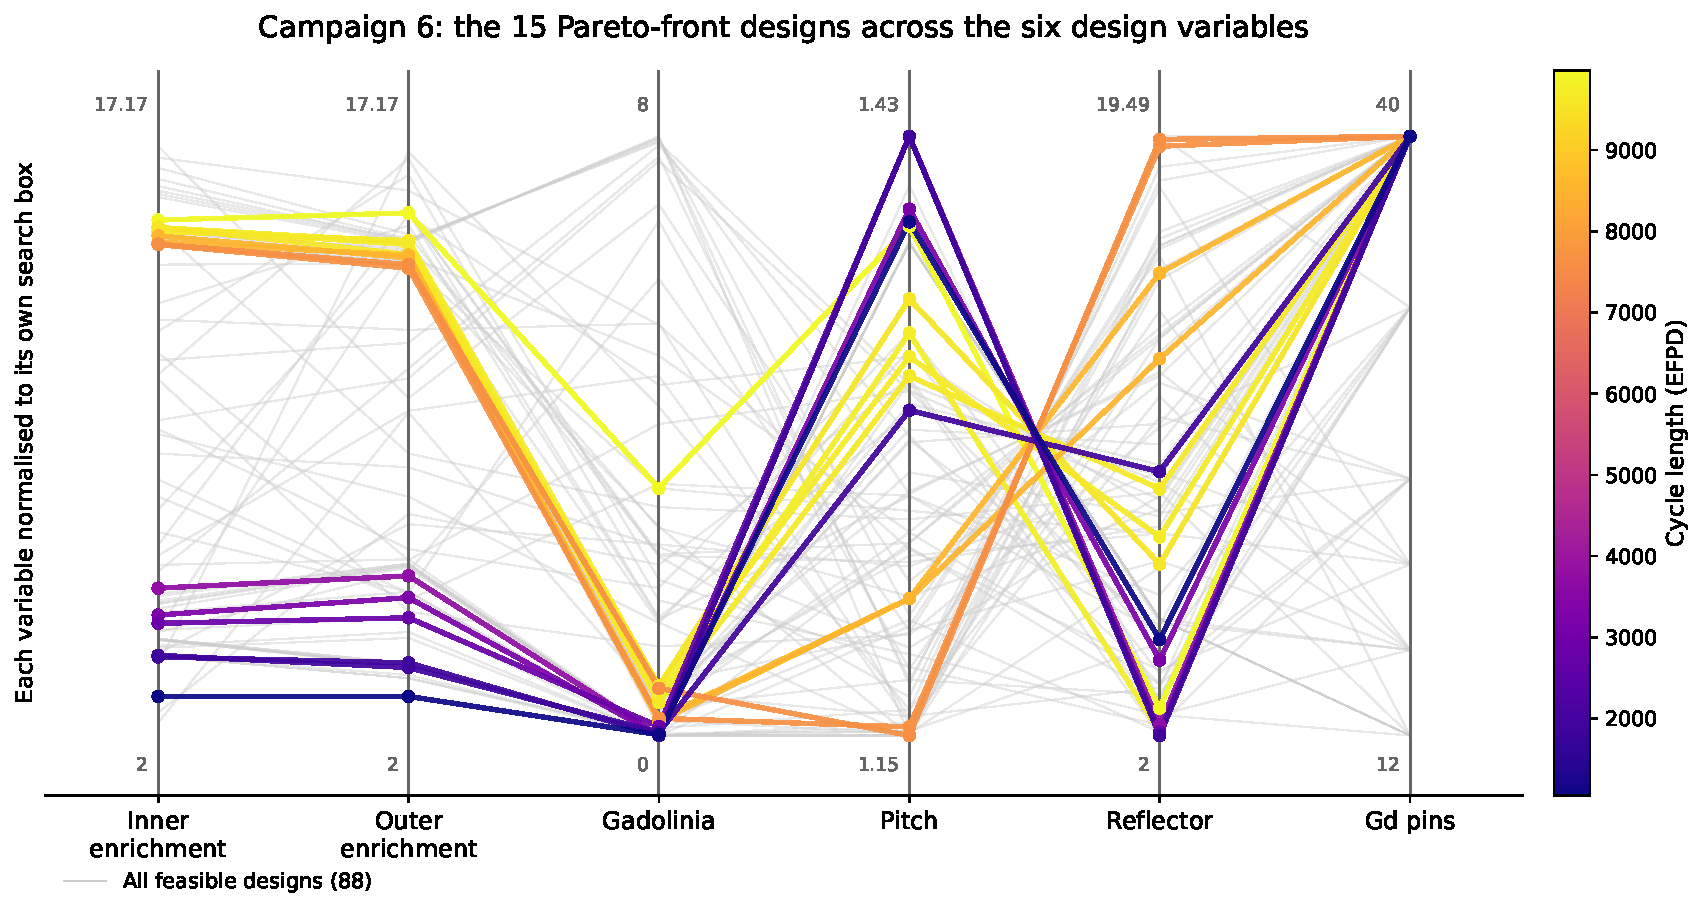
\includegraphics[width=\linewidth]{images/c6_vars_parallel}
  \caption{The fifteen Campaign 6 Pareto-front designs in parallel coordinates.}
  \label{fig:c6-parallel}
\end{figure}

The front is diverse in four of the six variables and unanimous in
one. The pitch spans its entire box, the reflector spans 99 per cent
of its box, the enrichments span about 80 per cent, and the gadolinia
content spans 0 to 3.30~wt\%. Every front design, without exception,
carries 40 gadolinium-bearing pins, the maximum of the ladder,
selected from a design of experiments that sampled all six ladder
values. The trade the optimiser found is many pins at low
concentration rather than few pins at high concentration. The archive
contains the concentrated alternative, a design at 7.92~wt\% in 16
pins reaching \num{9625} effective full power days, and it is
dominated by the dilute champion by \num{50} days and 0.006 in
peaking.

The preference for many dilute pins follows from the self-shielding
of the absorber. A poisoned pellet is optically black to thermal
neutrons, so absorption proceeds from its surface inward and the rate
at which the poison burns out is set by the surface exposed rather
than by the mass loaded (Section~\ref{sec:bg-gd}). Forty pins at low
concentration expose more surface than sixteen at high concentration,
so they burn out early and little absorber survives to the end of
cycle, whereas concentrated pins burn out late and carry a larger
residual penalty. The mechanism is self-shielding: the gadolinium atoms
in the outer layer of a pellet transmute faster than those
inside~\cite{gd_enriched_2021}. The early burnout has a cost
that this campaign did not score: it releases the hold-down before the
fuel has depleted and produces the reactivity hump analysed in
Section~\ref{sec:res-c9-gd}. Concentrated pins also depress their
own power more deeply, which loads their neighbours and raises the
peaking, in the direction that the 0.006 difference records.

The parallel-coordinates view also shows the vessel-fit coupling
directly. The long-cycle designs pair narrow pitch with a thick
reflector or wide pitch with a thin one, crossing between the two
axes, which is Equation~\eqref{eq:renv} acting as the budget it is.

\subsection{Variable influence and constraint activity}
\label{sec:res-c6-influence}

Figure~\ref{fig:c6-influence} shows the influence of each design variable
on the cycle length over the archive, coloured by the zoned-core peaking
factor and with the Pareto-front designs ringed. Each panel reports the
Spearman rank correlation of the variable with both objectives over the
feasible designs, and Table~\ref{tab:c6-spearman} collects the same
correlations.

\begin{figure}[htbp]
  \centering
  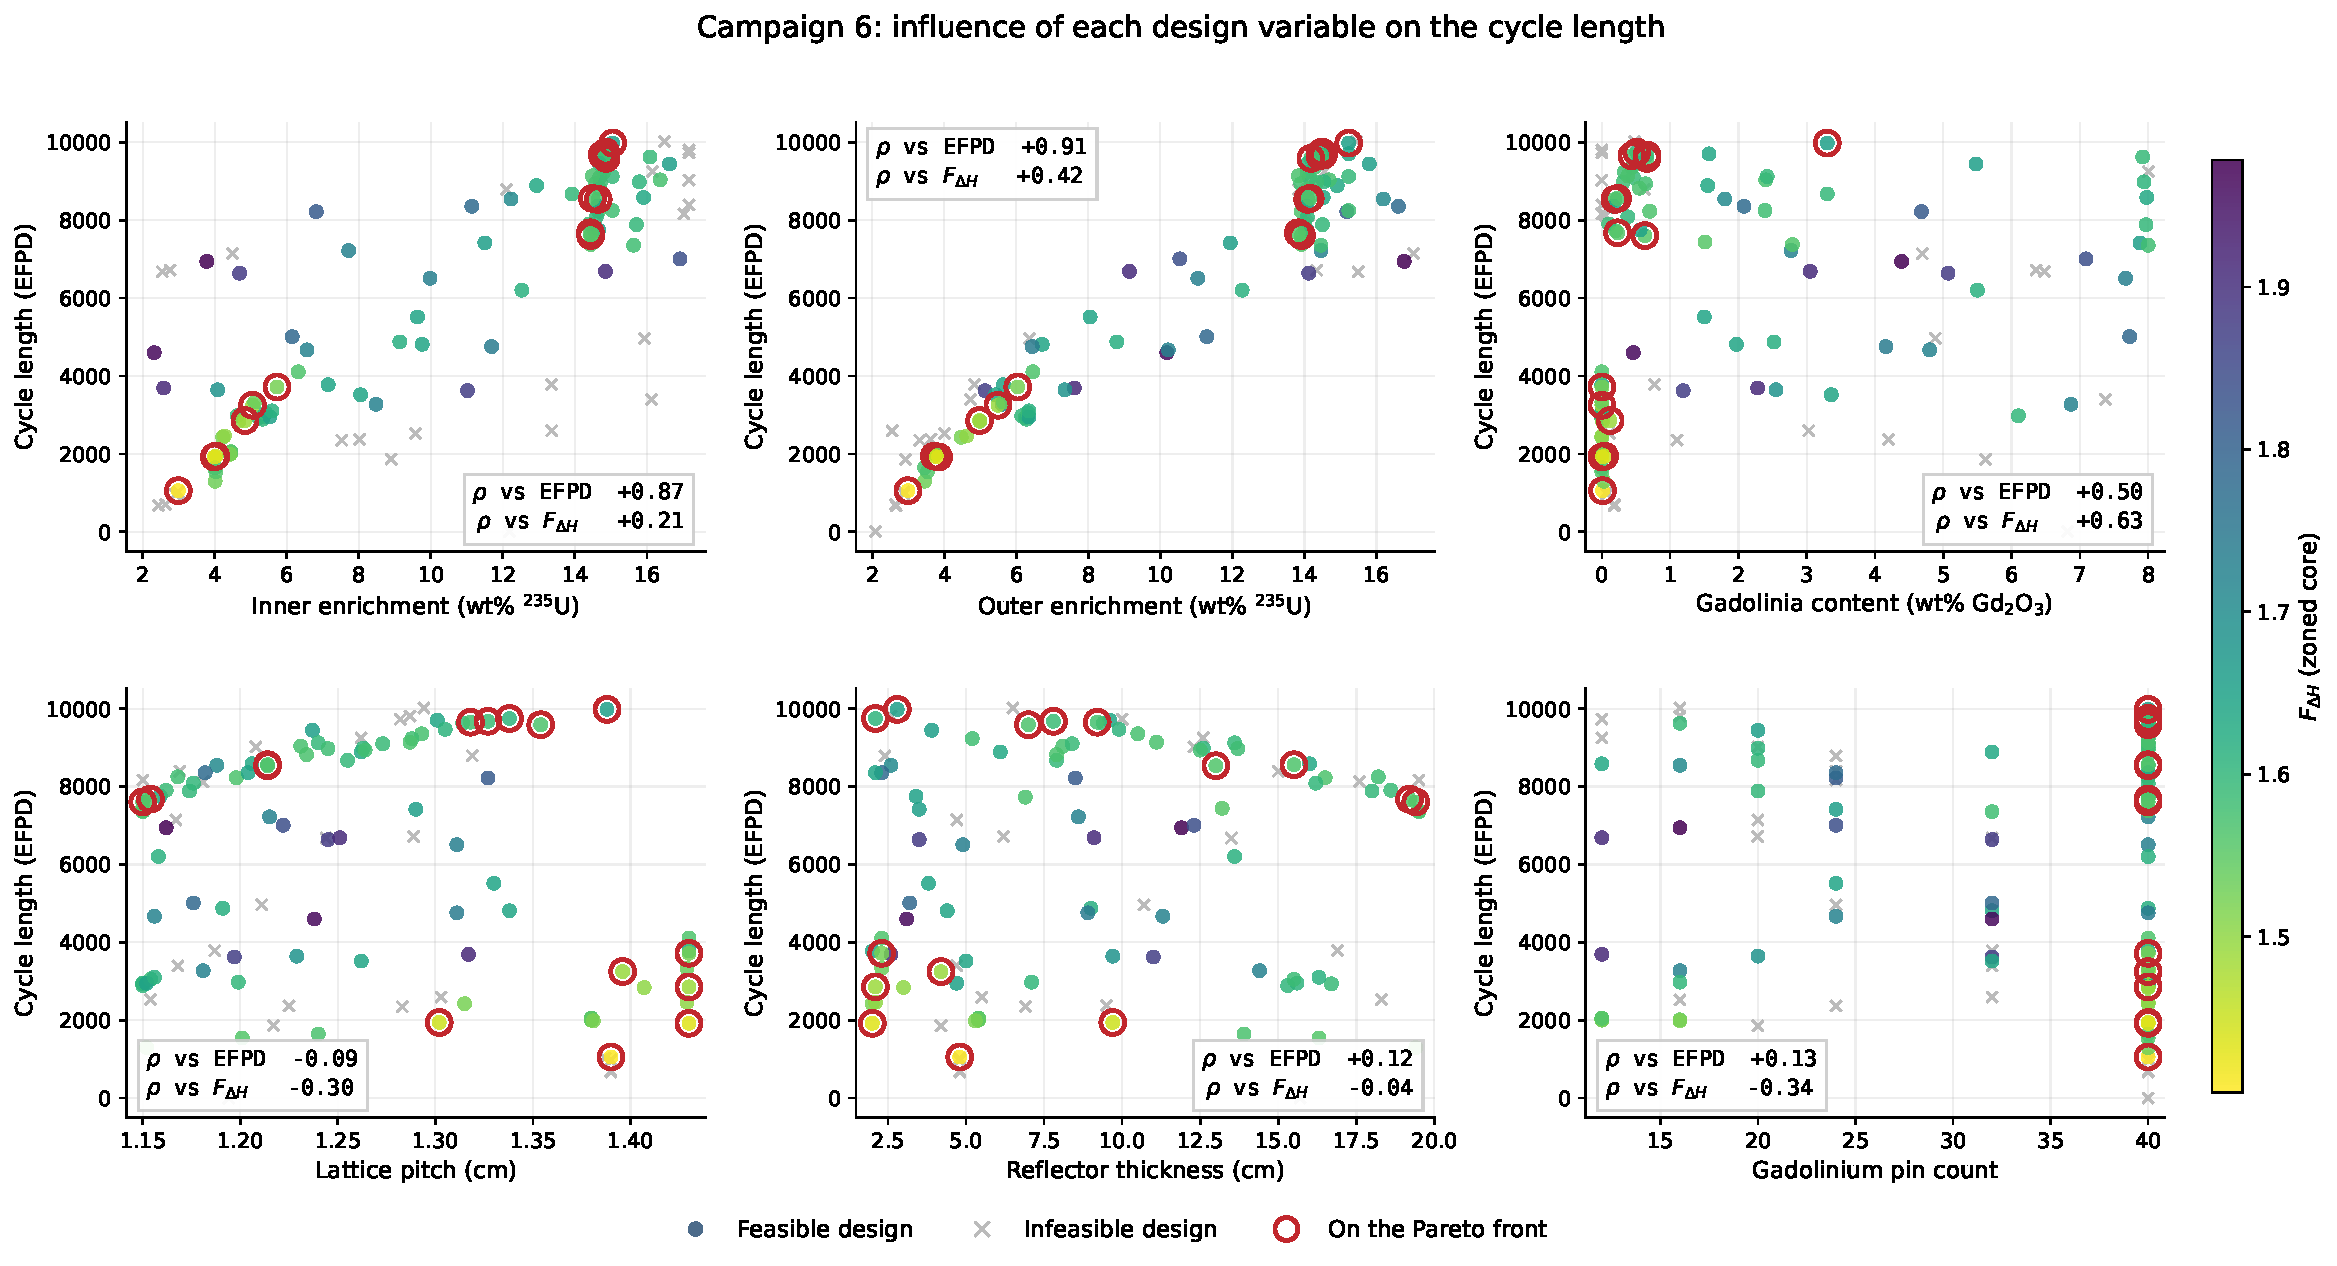
\includegraphics[width=\linewidth]{images/c6_vars_influence}
  \caption{Influence of each design variable on the cycle length over the Campaign 6 archive.}
  \label{fig:c6-influence}
\end{figure}

\begin{table}[htbp]
  \centering
  \caption{Spearman rank correlation of each design variable with the
  two objectives, over the 88 feasible designs of Campaign 6.}
  \label{tab:c6-spearman}
  \begin{tabular}{lcc}
    \toprule
    Variable & vs cycle length & vs $F_{\Delta H}$ \\
    \midrule
    $e_\mathrm{out}$  & $+0.905$ & $+0.422$ \\
    $e_\mathrm{in}$   & $+0.866$ & $+0.209$ \\
    gd                & $+0.498$ & $+0.633$ \\
    $n_\mathrm{Gd}$   & $+0.132$ & $-0.345$ \\
    $t_\mathrm{refl}$ & $+0.122$ & $-0.044$ \\
    $p$               & $-0.088$ & $-0.301$ \\
    \bottomrule
  \end{tabular}
\end{table}

Three readings are supported. First, enrichment dominates the cycle
length and nothing else approaches it, with the outer zone the
stronger of the two, consistent with the peripheral weighting of the
zoned map. Second, the gadolinia content correlates positively with
both objectives at once, which is not a physical benefit of the
absorber but a constraint-induced coupling. The absorber is present
only where the enrichment is high, because only there does the
reactivity ceiling demand it, so its apparent association with long
cycles is inherited from the enrichment. Third, the pitch and the
reflector barely move the cycle length while both act on the peaking,
which matches their role as radial-budget variables under the
vessel-fit coupling rather than as reactivity variables.

The reflector keeps that role in Campaign 8. With the pitch
fixed and the reflector capped at \SI{5.66}{cm}, the leakage-corrected
reactivity target moves by only about \SI{200}{pcm} over the whole
reflector range (Section~\ref{sec:meth-lax}), so in Campaign 8 the
reflector thickness acts on the radial power shape alone.

Figure~\ref{fig:c6-constraints} shows the reactivity constraint activity
across the archive.

\begin{figure}[htbp]
  \centering
  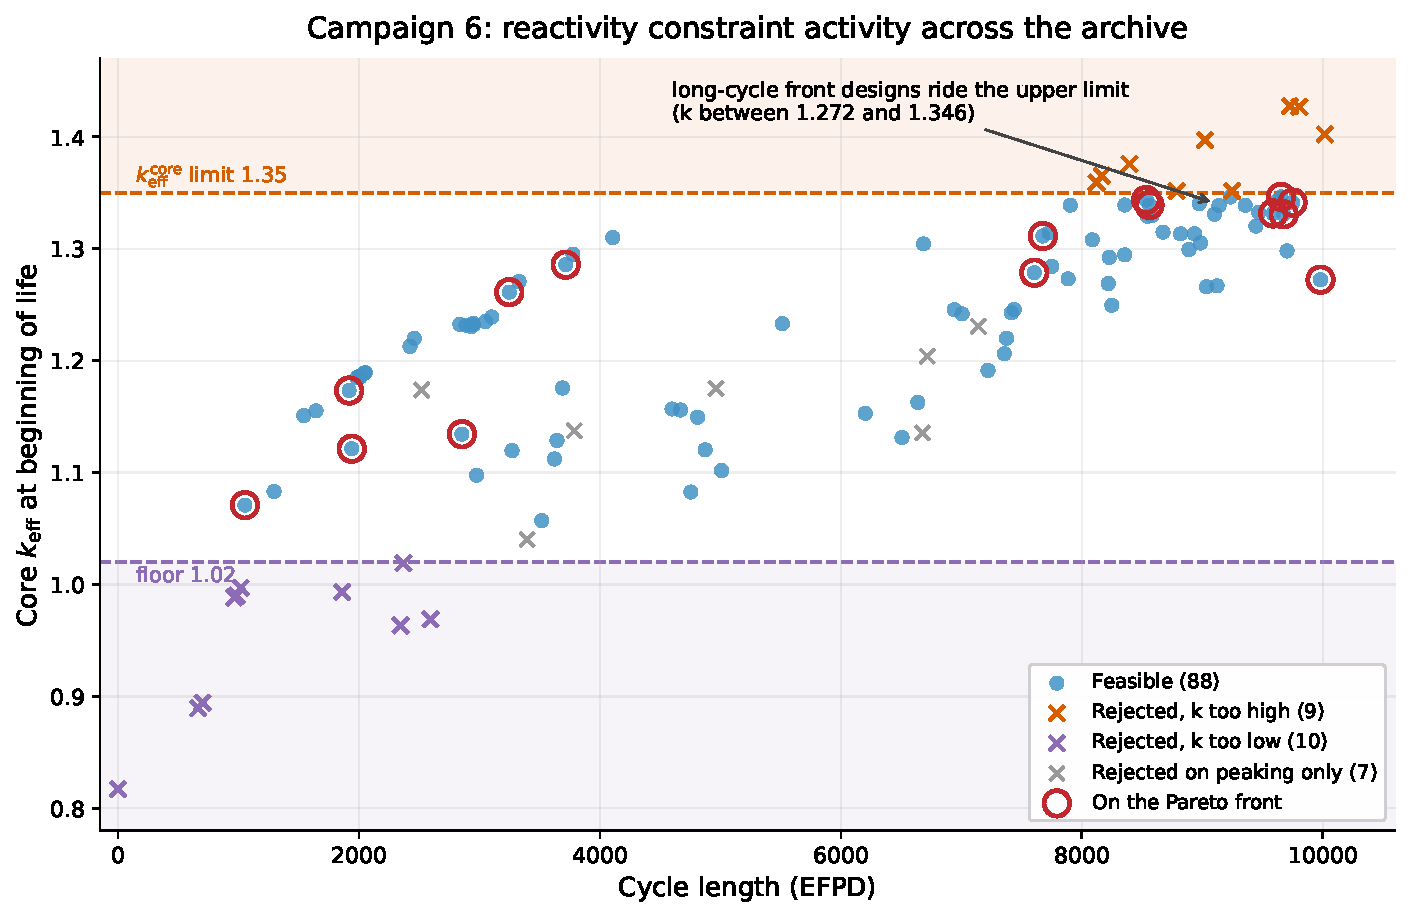
\includegraphics[width=0.92\linewidth]{images/c6_extra_constraints}
  \caption{Reactivity constraint activity across the Campaign 6 archive.}
  \label{fig:c6-constraints}
\end{figure}

The constraint activity closes the argument. Of the 26 rejections,
nine exceed the reactivity ceiling, ten fall below the floor of 1.02 as
genuinely subcritical or barely critical cores, and seven fail the
peaking limit alone. The long-cycle end of the front rides
the ceiling, with the nine designs beyond \num{7000} effective full
power days holding $k_\mathrm{eff}^\mathrm{core}$ between 1.272 and
1.346. The upper reactivity bound, not the peaking limit and not the
enrichment cap, is the active constraint that terminates the front on
the long-cycle side.

\subsection{The discharge-burnup screen}
\label{sec:res-c6-bscreen}

The depletion horizon of \SI{100}{\mega\watt\day\per\kilo\gram} is a
numerical device, and the discharge-qualification screen remains
$B_\mathrm{ATF} = \SI{75}{\mega\watt\day\per\kilo\gram}$, applied here
at candidate selection as Section~\ref{sec:meth-atf} prescribes.

The screen is consequential. Of the 88 feasible designs, 51 satisfy
it, and the nine long-cycle front designs beyond \num{7677} effective
full power days all exceed it, at end-of-cycle burnups between 75.9
and \SI{99.6}{\mega\watt\day\per\kilo\gram}. The screened front
therefore differs from the unscreened one at the long-cycle end, as
Table~\ref{tab:c6-front-screened} shows.

\begin{table}[htbp]
  \centering
  \caption{The Pareto front of the feasible designs satisfying the
  discharge-qualification screen
  $B_\mathrm{EOC} \le \SI{75}{\mega\watt\day\per\kilo\gram}$.}
  \label{tab:c6-front-screened}
  \begin{tabular}{cccccc}
    \toprule
    Index & EFPD & $F_{\Delta H}$ & $k_\mathrm{eff}^\mathrm{core}$ &
    $B_\mathrm{EOC}$ (MWd/kg) & gd (wt\%) \\
    \midrule
    101 & 7439 & 1.5564 & 1.24564 & 74.3 & 1.51 \\
     91 & 3717 & 1.5241 & 1.28575 & 37.1 & 0.00 \\
     85 & 3248 & 1.4938 & 1.26117 & 32.4 & 0.00 \\
    110 & 2855 & 1.4894 & 1.13427 & 28.5 & 0.12 \\
     69 & 1941 & 1.4480 & 1.12128 & 19.4 & 0.04 \\
    107 & 1919 & 1.4317 & 1.17329 & 19.2 & 0.00 \\
     59 & 1054 & 1.4041 & 1.07087 & 10.5 & 0.01 \\
    \bottomrule
  \end{tabular}
\end{table}

Under the screen the champion is design 101, at \num{7439} effective
full power days, $F_{\Delta H} = 1.5564$ and an end-of-cycle burnup of
\SI{74.3}{\mega\watt\day\per\kilo\gram}, which uses 99 per cent of the
qualification allowance. Its pitch of \SI{1.150}{cm} places it in the
guide-tube band of Section~\ref{sec:res-c7-limits}, so its peaking
value is qualified. The unscreened long-cycle designs, including
design 94, are conditional results. They quantify what the design
space offers if discharge burnups beyond
\SI{75}{\mega\watt\day\per\kilo\gram} can be qualified, and they are
reported as such rather than as candidates.

Neither champion is carried forward. Campaign 7 showed that the
reactivity ceiling of this campaign is a proxy for a controllability
requirement that must be measured (Section~\ref{sec:res-c7-screens}),
and Campaign 8 rebuilt the design space on that finding. The Campaign
6 designs are therefore the resolved front of a superseded
formulation, and the candidate list of this work is that of
Section~\ref{sec:res-c8-limits}.

\subsection{Comparison with the earlier campaigns and residual
caveats}
\label{sec:res-c6-compare}

Against the core-level results of the earlier campaigns the
improvement is large, and it decomposes cleanly into a bookkeeping
part and a physical part.

\begin{enumerate}
  \item In the Campaign 3 core validation, zero of 36 designs
        satisfied the peaking limit and the minimum core value was
        $2.013 \pm 0.018$. In Campaign 5 the closest approach was
        2.0012. In Campaign 6 the feasible median is 1.59 and the
        front reaches 1.4041.

  \item The reactivity basis change and the raised horizon are
        bookkeeping. The Campaign 5 re-scoring of
        Section~\ref{sec:res-c5-kbasis} quantifies the basis change
        in isolation, and the horizon acts only on censoring.

  \item The peaking collapse is attributable to the zoning alone,
        because $F_{\Delta H}$ is a beginning-of-life quantity that
        neither bookkeeping change can touch. The evaluator-zoned map
        of Section~\ref{sec:meth-zoning} is therefore the physically
        real driver of Campaign 6 feasibility.
\end{enumerate}

The enrichment landscape of the front is itself a result. The zoned
peripheral enrichments of the front span 3.4 to 17.5~wt\%, enclosing
the mid-single-digit values associated with first cores of this
reactor class and approaching, without being told to, the
low-enriched-uranium cap. The comparison with the reported refuelling
interval and the reported enrichment of the prototype is made once,
on the Campaign 8 front, in Section~\ref{sec:res-c8-mission}.

Campaign 7 and the axial study then showed that the high-enrichment end
of this front is not controllable by the regulating banks. Design 86,
at 14.4~wt\% in the volume-weighted sense, remains supercritical with
all regulating banks inserted in two and in three dimensions
(Section~\ref{sec:meth-lax}). The enrichment cap of the final campaign
is therefore a consequence of the control screen and not of the
low-enriched-uranium limit.

Five caveats bound the claims of this section.

\begin{enumerate}
  \item Every Campaign 6 cycle length is an exploration-tier value at
        the $4\,000\times60$ depletion fidelity of
        Table~\ref{tab:fidelity}, and is not directly comparable with
        the Campaign 3 to 5 values at $16\,000\times120$. The
        finalists are not re-scored, for the reason given in
        Section~\ref{sec:res-c6-bscreen}. Feasibility and every
        peaking value are unaffected, because the core solve is at
        full fidelity throughout.

  \item Every Campaign 6 cycle length is a two-dimensional value. The
        axial study of Section~\ref{sec:meth-lax}, performed on six
        designs of this campaign, measured the axial leakage factor at
        \num{1.0282} to \num{1.0298}, about \SI{3000}{pcm}, which at
        the end-of-cycle reactivity slopes of these designs is roughly
        450 to 500 effective full power days. The cycle lengths of
        Table~\ref{tab:c6-front} are overstated by that amount
        relative to a finite-height core, uniformly, so the ordering
        of the front is unaffected.

  \item Four front designs and the discharge-screen champion lie in
        the guide-tube band below \SI{1.2242}{cm}
        (Section~\ref{sec:res-c6-front}).

  \item The Campaign 6 depletion runs under the corrected restart
        configuration of Section~\ref{sec:restart_defect}, verified in
        the campaign metadata, so its burnups are free of the defect
        that affected Campaigns 3 to 5.

  \item The frozen hypervolume reference was constructed from a
        two-design front and proved blind to the entire short-cycle
        half of the trade. The convergence claim of this campaign
        therefore rests on the frozen metric, the full-range metric,
        the relaxation cascade and the margin-feasible count jointly,
        and Figure~\ref{fig:c6-convergence} reports the first two side
        by side. Reporting a single hypervolume number against a
        single reference is, on this evidence, not a sufficient
        convergence statement for a front whose extent is unknown in
        advance~\cite{zitzler_2003_performance}.
\end{enumerate}

What carries forward from this campaign is its architecture rather
than its designs. The four-part acquisition of
Section~\ref{sec:meth-acq}, the surrogate search setting, the two
health indicators of the stopping rule, the core-basis reactivity
window and the evaluator-level zoning are all retained by Campaigns 7
and 8. The designs themselves are superseded, first by the measured
controllability screen and then by the fixed-pitch design space.

\openpoint{Section~\ref{sec:res-c7-uncertainty} attributes to this
section an entropy study that bounded the systematic shift of the
core peaking factor at $\pm 0.02$. That study is not documented here.
Either insert its text into this section or redirect the reference to
where the study is reported.}

\section{Campaign 7: the controllability screen}
\label{sec:res-c7}

Campaign 6 closed with a front whose long-cycle end rode the
reactivity ceiling, and with the observation that the ceiling of 1.35
proxied controllable excess reactivity without a rod model. Campaign 7
replaces the proxy by a measurement. Every evaluation now solves the
beginning-of-life core a second time with the sixteen regulating-bank
control rod assemblies inserted, and the resulting eigenvalue enters the
constraint set directly. The campaign ran 60 evaluations on the AWS
instance in \SI{15.82}{h}, and every one of them completed without
error.

\subsection{The one change and its two consequences}
\label{sec:res-c7-basis}

The constraint added is the controllability screen of
Section~\ref{sec:meth-ctrl}.

\begin{equation}
g_\mathrm{ctrl}(\mathbf{x}) = k_\mathrm{RE}(\mathbf{x}) - (1 - \Delta\rho_\mathrm{op}) \le 0
\label{eq:g-ctrl}
\end{equation}

\noindent where the symbols have the following meaning.

\begin{itemize}
  \item $k_\mathrm{RE}$ is the effective multiplication factor of the
        32-assembly core at beginning of life with the sixteen
        regulating-bank assemblies inserted and the sixteen
        shutdown-bank assemblies withdrawn, dimensionless. It is not
        the all-rods-in state of Section~\ref{sec:meth-ctrl}.

  \item $\Delta\rho_\mathrm{op}$ is the operating subcriticality margin
        demanded of the regulating banks, \num{0.01} in units of $k$,
        that is \SI{1000}{pcm}.

  \item $\mathbf{x}$ is the design vector.
\end{itemize}

Two settings changed with it. The reactivity ceiling was lowered from
1.35 to 1.126, a value derived before the campaign from the smallest
regulating-bank worth measured on eight Campaign 6 designs, and the
enrichment cap was lowered to \SI{12}{wt\%} on the as-built peripheral
ring, giving a search box of 3.0 to \SI{10.43}{wt\%}. Both were
intended as consequences of the controllability requirement rather than
as independent changes, and the campaign tests whether they were
consistent with the measurement they were meant to anticipate.

\subsection{Design of experiments and the three infill blocks}
\label{sec:res-c7-blocks}

The campaign ran a design of experiments of 42 followed by three infill
blocks of six. Table~\ref{tab:c7-blocks} records the outcome of each
block and Figure~\ref{fig:c7-diversity} its diversity, measured as the
spread of each design variable within the block as a fraction of the
range spanned by the whole archive. In the table the hypervolume is the
frozen-reference value written at each block boundary, and the spread is
listed for the four non-geometric variables. Infill blocks 1 and 3 vary
only the pitch and the reflector thickness, and neither returned a
feasible design.

\begin{table}[htbp]
  \centering
  \caption{Campaign 7 blocks.}
  \label{tab:c7-blocks}
  \begin{tabular}{lccll}
    \toprule
    Block & Designs & Feasible & Hypervolume & Spread in $e_\mathrm{in}$, $e_\mathrm{out}$, $w_\mathrm{Gd}$, $n_\mathrm{Gd}$ \\
    \midrule
    DOE      & 42 & 13 & 773.7 & 0.98 to 1.00 \\
    Infill 1 &  6 &  0 & 773.7 & 0.000 to 0.002 \\
    Infill 2 &  6 &  3 & 996.5 & 0.07 to 0.29 \\
    Infill 3 &  6 &  0 & 996.5 & 0.015 to 0.13 \\
    \bottomrule
  \end{tabular}
\end{table}

\begin{figure}[htbp]
  \centering
  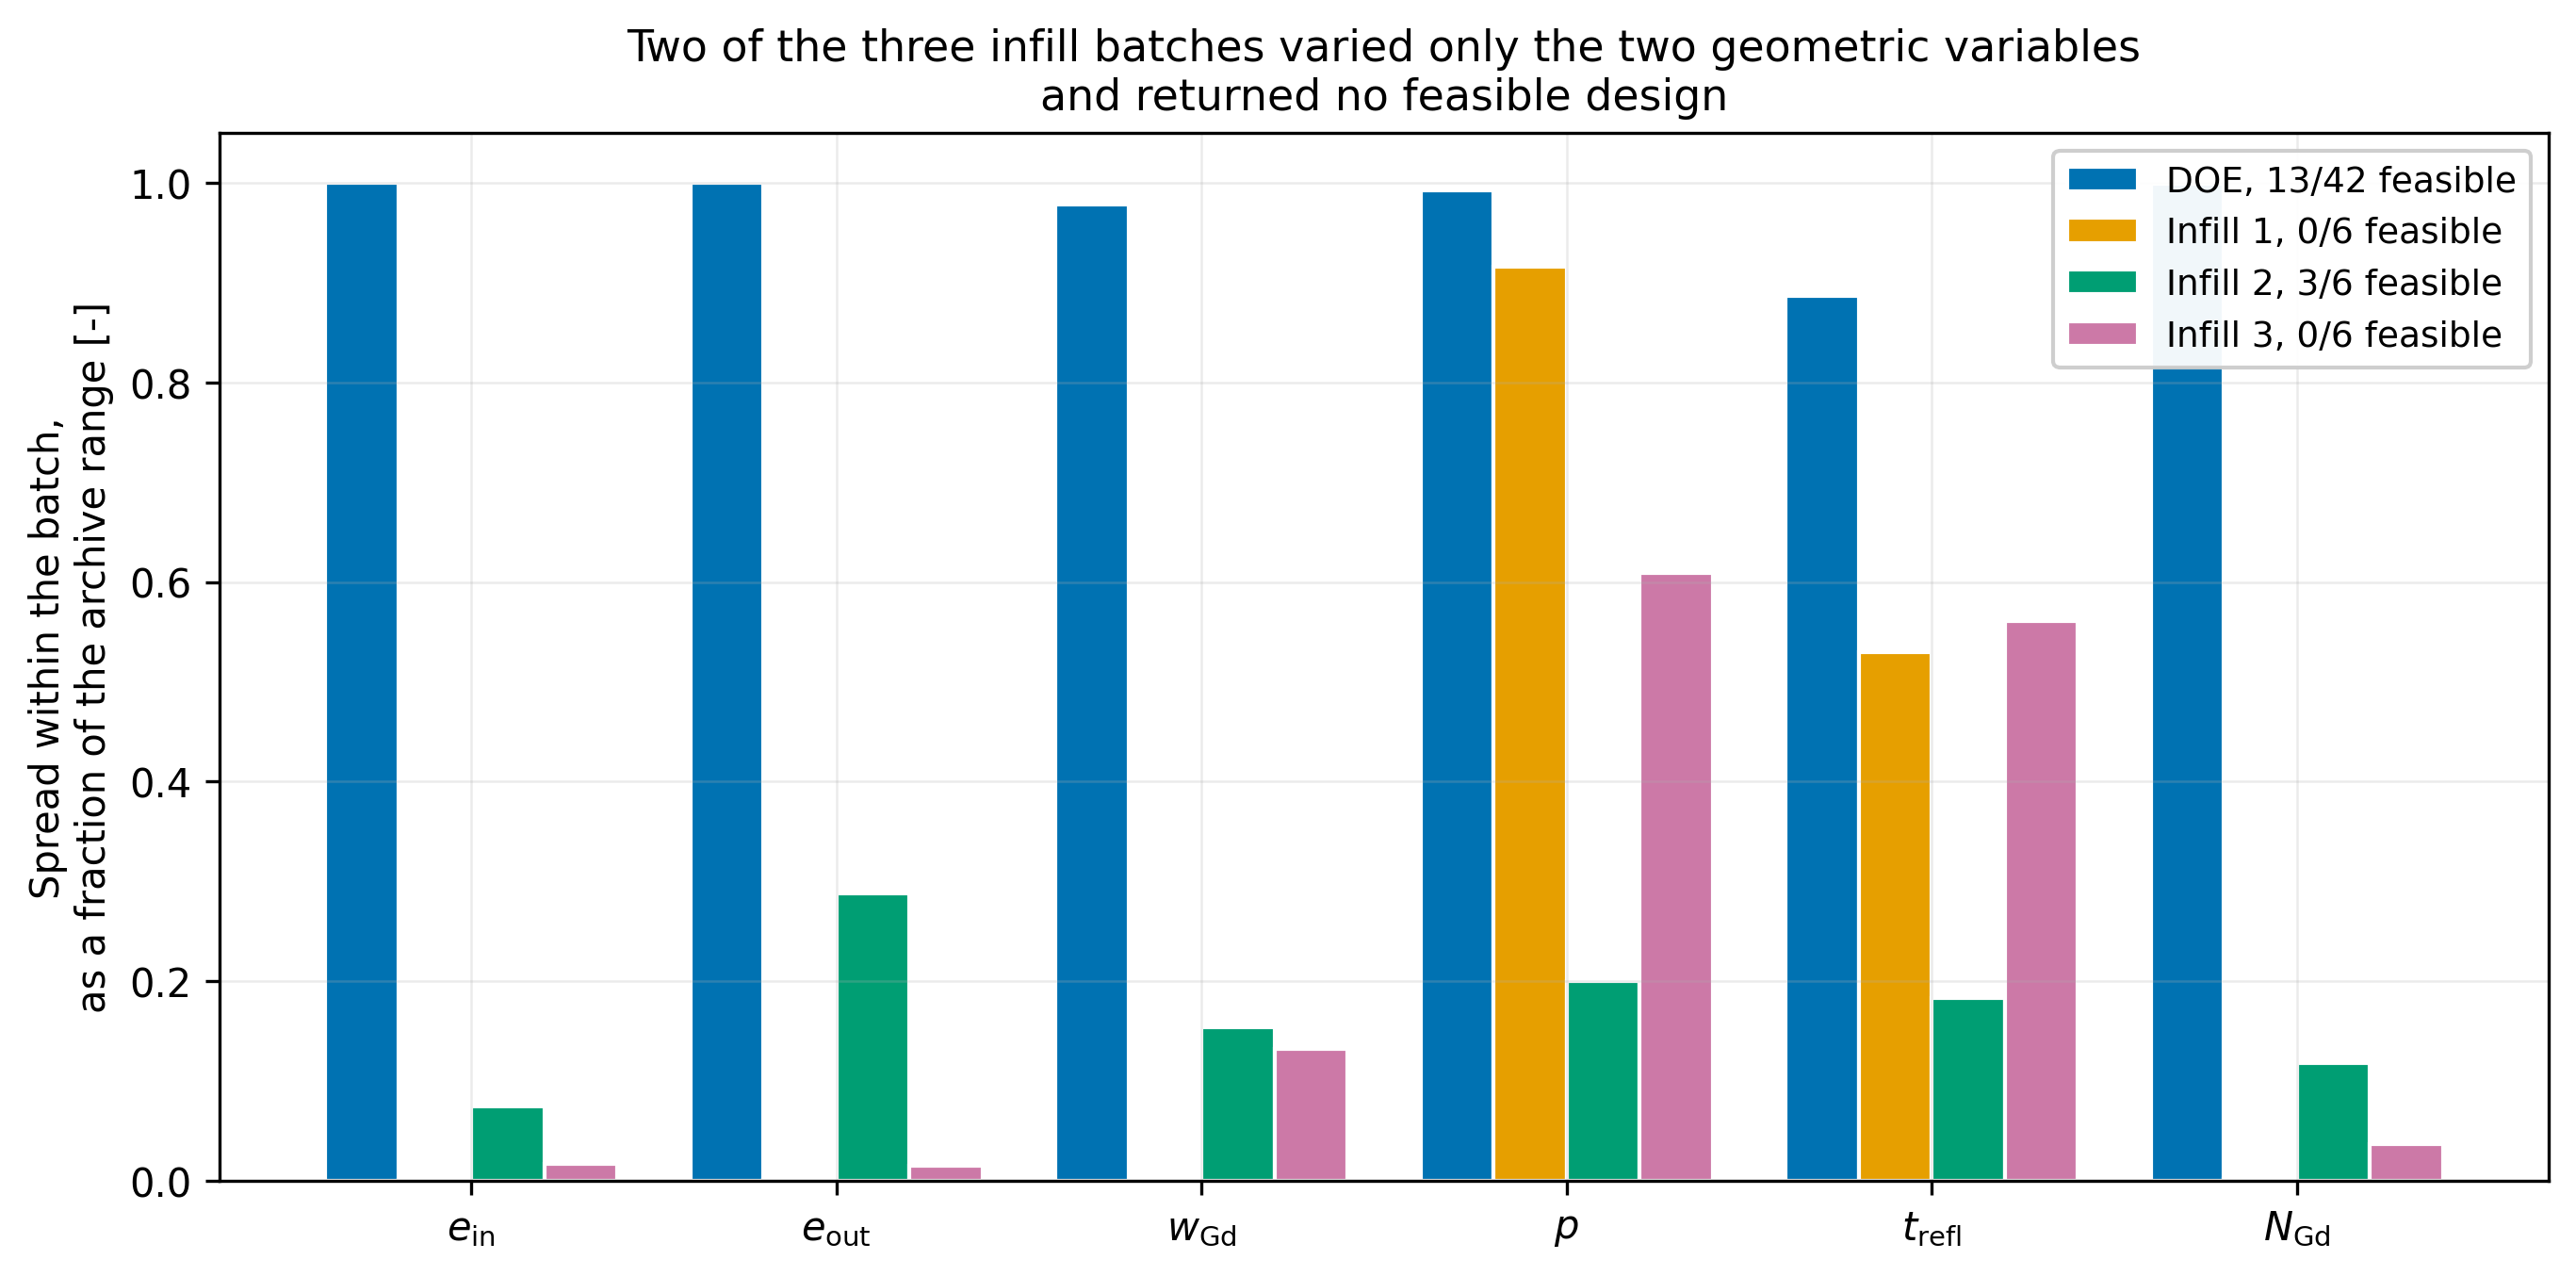
\includegraphics[width=\linewidth]{images/c7_infill_diversity}
  \caption{Within-block spread of each design variable in Campaign 7, as a fraction of the archive range.}
  \label{fig:c7-diversity}
\end{figure}

Two of the three infill blocks collapsed. In block 1 the six designs
share one enrichment pair, \num{5.09} and \SI{4.04}{wt\%}, exactly zero
gadolinia and 24 poisoned pins, and differ only in pitch and reflector
thickness. In block 3 the same pattern recurs at \num{8.13} and
\SI{7.33}{wt\%} with 32 pins. All twelve designs of the two blocks
failed the reactivity ceiling.

The cause is a configuration regression, not a new defect. The
acquisition ran with a minimum separation of 0.05 and a feasibility
margin of 1.0 standard deviation, the default values of the launcher,
where Campaign 6 had established 0.14 and 1.5 in
Section~\ref{sec:res-c6-margin}. The two collapsed blocks satisfied the
separation rule as coded, with pairwise separations of 0.059 to 0.089,
because the rule averages over all six variables and two of them
supplied the whole distance. A per-variable minimum spread would have
rejected both batches.

The consequence for the convergence record is that the flat
hypervolume of block 3 is not a stopping signal. Under the Campaign 6
rule a zero gain counts toward stopping only when the acquisition is
functioning, and block 3 demonstrably was not. The campaign therefore
ends with an unconverged front, and its value lies in the constraint
measurements rather than in the front itself.

\subsection{Feasibility and the nesting of the two screens}
\label{sec:res-c7-screens}

Of the 60 designs, 16 are feasible against all six constraints, a
fraction of \SI{26.7}{\%} against \SI{67}{\%} in the Campaign 6 design
of experiments. Table~\ref{tab:c7-nesting} gives the constraint census,
and Figure~\ref{fig:c7-screens} shows the two reactivity screens in the
plane of the unrodded and the rodded core eigenvalues, with the fourteen
designs rejected only by the derived ceiling marked by open circles.
No design fails the enrichment or the geometric constraint, two fail
the peaking limit, nine fall below the reactivity floor, 34 exceed the
ceiling and 20 fail the controllability screen.

\begin{table}[htbp]
  \centering
  \caption{Constraint census of Campaign 7 and the joint activity of the two reactivity screens.}
  \label{tab:c7-nesting}
  \begin{tabular}{lc}
    \toprule
    Outcome & Designs \\
    \midrule
    Fail $g_{k\max}$ at 1.126                      & 34 \\
    Fail $g_\mathrm{ctrl}$                         & 20 \\
    Fail $g_\mathrm{ctrl}$ and pass $g_{k\max}$    &  0 \\
    Fail $g_{k\max}$ and pass $g_\mathrm{ctrl}$    & 14 \\
    Pass every constraint except $g_{k\max}$       & 14 \\
    Feasible on all six                            & 16 \\
    \bottomrule
  \end{tabular}
\end{table}

\begin{figure}[htbp]
  \centering
  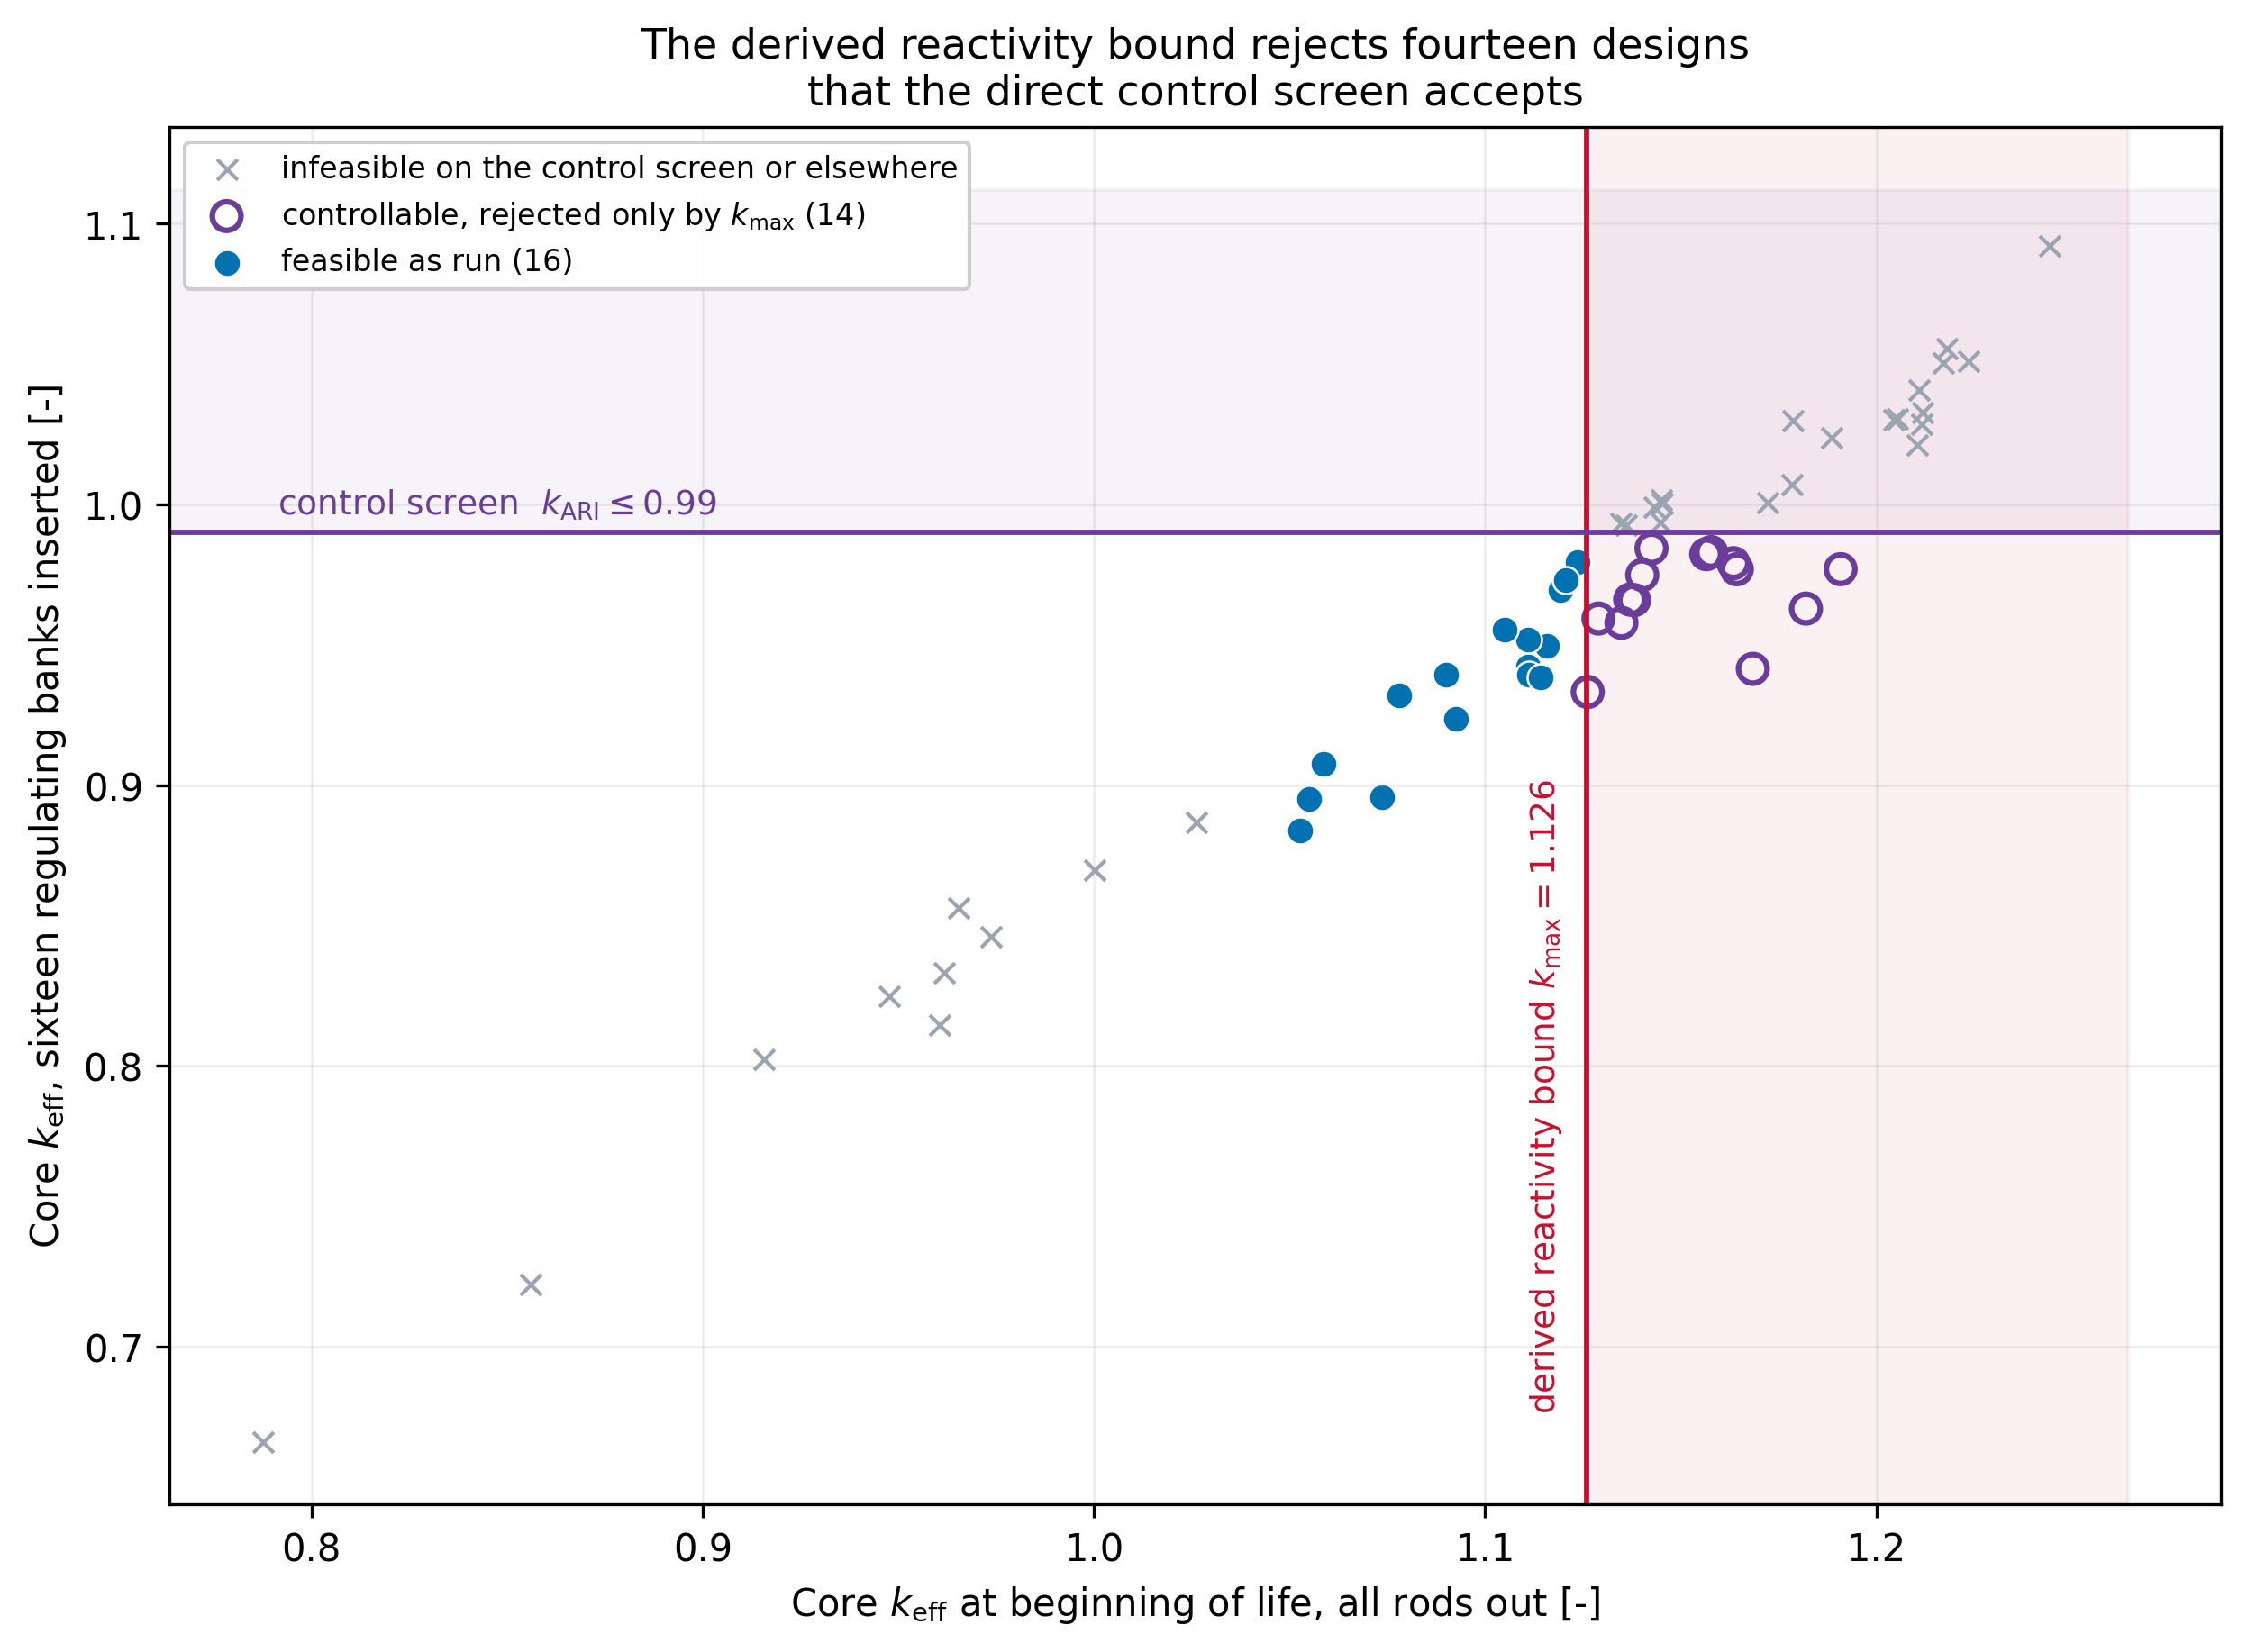
\includegraphics[width=0.9\linewidth]{images/c7_ctrl_screen}
  \caption{The two reactivity screens of Campaign 7 in the plane of the unrodded and the all-regulating-banks-in core eigenvalues.}
  \label{fig:c7-screens}
\end{figure}

The two screens are nested. Not one design in the archive fails the
control screen without also failing the derived ceiling, and fourteen
designs fail the ceiling while their own measured bank worth shows them
controllable at the stated margin. Figure~\ref{fig:c7-screens} shows
the nesting directly. The ceiling of 1.126 therefore did no work that
the measurement did not do, and it discarded fourteen evaluations that
the measurement would have kept.

The derivation explains why. The eight Campaign 6 designs from which
1.126 was obtained had worths between \num{12174} and
\SI{12718}{pcm}, a spread of four per cent. The 60 designs of this
campaign span \num{10936} to \SI{22699}{pcm}, a factor of two. Eight
near-identical designs under-sampled the variability by an order of
magnitude, and the resulting bound is at once too tight where it
matters and not conservative in general. Restricted to the 22 designs
with an unrodded eigenvalue between 1.09 and 1.17, the smallest
measured worth of \SI{14126}{pcm} implies a ceiling of 1.151, while the
smallest worth in the whole archive implies 1.110.

The front reflects the same fact. As run, the feasible non-dominated set
holds three designs, all from infill block 2. With the derived ceiling
removed and the measured control screen retained, the feasible set grows
from 16 to 30 designs, the front doubles to six, the peaking floor moves
from 1.565 to 1.525, and the hypervolume against the frozen reference
rises from 996.5 to 1054.1, a gain of \SI{5.8}{\%}. Three of the six
designs come from infill block 3, the block that under the ceiling
contributed nothing. Table~\ref{tab:c7-front} lists both fronts and
Figure~\ref{fig:c7-pareto} places them in the objective plane.
Designs 48, 53 and 49 form the front as run, and all six form it when the
measured control screen alone governs reactivity. The bank worth in the
table is the difference between the unrodded and the all-banks-in
eigenvalues. In the figure filled markers are feasible as run and open
circles are controllable designs rejected only by the derived ceiling.
The solid front is the one the campaign reported, and the dashed front is
the one the measured control screen supports.

\begin{table}[htbp]
  \centering
  \small
  \caption{The Campaign 7 front under the two screening rules.}
  \label{tab:c7-front}
  \begin{tabular}{ccccccccccc}
    \toprule
    Design & EFPD & $F_{\Delta H}$ & $e_\mathrm{in}$ & $e_\mathrm{out}$ & $w_\mathrm{Gd}$ & $p$ & $t_\mathrm{refl}$ & $n_\mathrm{Gd}$ & $k_\mathrm{eff}^\mathrm{core}$ & worth \\
           & [d] & [-] & [wt\%] & [wt\%] & [wt\%] & [cm] & [cm] & [-] & [-] & [pcm] \\
    \midrule
    59 & 3886 & 1.525 & 8.13 & 7.33 & 1.10 & 1.150 & 19.49 & 32 & 1.135 & 17699 \\
    57 & 4045 & 1.528 & 8.13 & 7.33 & 1.21 & 1.176 & 17.87 & 32 & 1.137 & 17094 \\
    55 & 4502 & 1.529 & 8.14 & 7.34 & 1.10 & 1.238 & 14.09 & 32 & 1.143 & 15815 \\
    48 & 4745 & 1.565 & 8.71 & 7.80 & 1.93 & 1.237 & 14.06 & 40 & 1.119 & 14970 \\
    53 & 4899 & 1.590 & 8.97 & 7.88 & 1.96 & 1.249 & 13.21 & 40 & 1.121 & 14734 \\
    49 & 5087 & 1.598 & 9.19 & 8.30 & 2.13 & 1.267 & 12.29 & 40 & 1.124 & 14416 \\
    \bottomrule
  \end{tabular}
\end{table}

\begin{figure}[htbp]
  \centering
  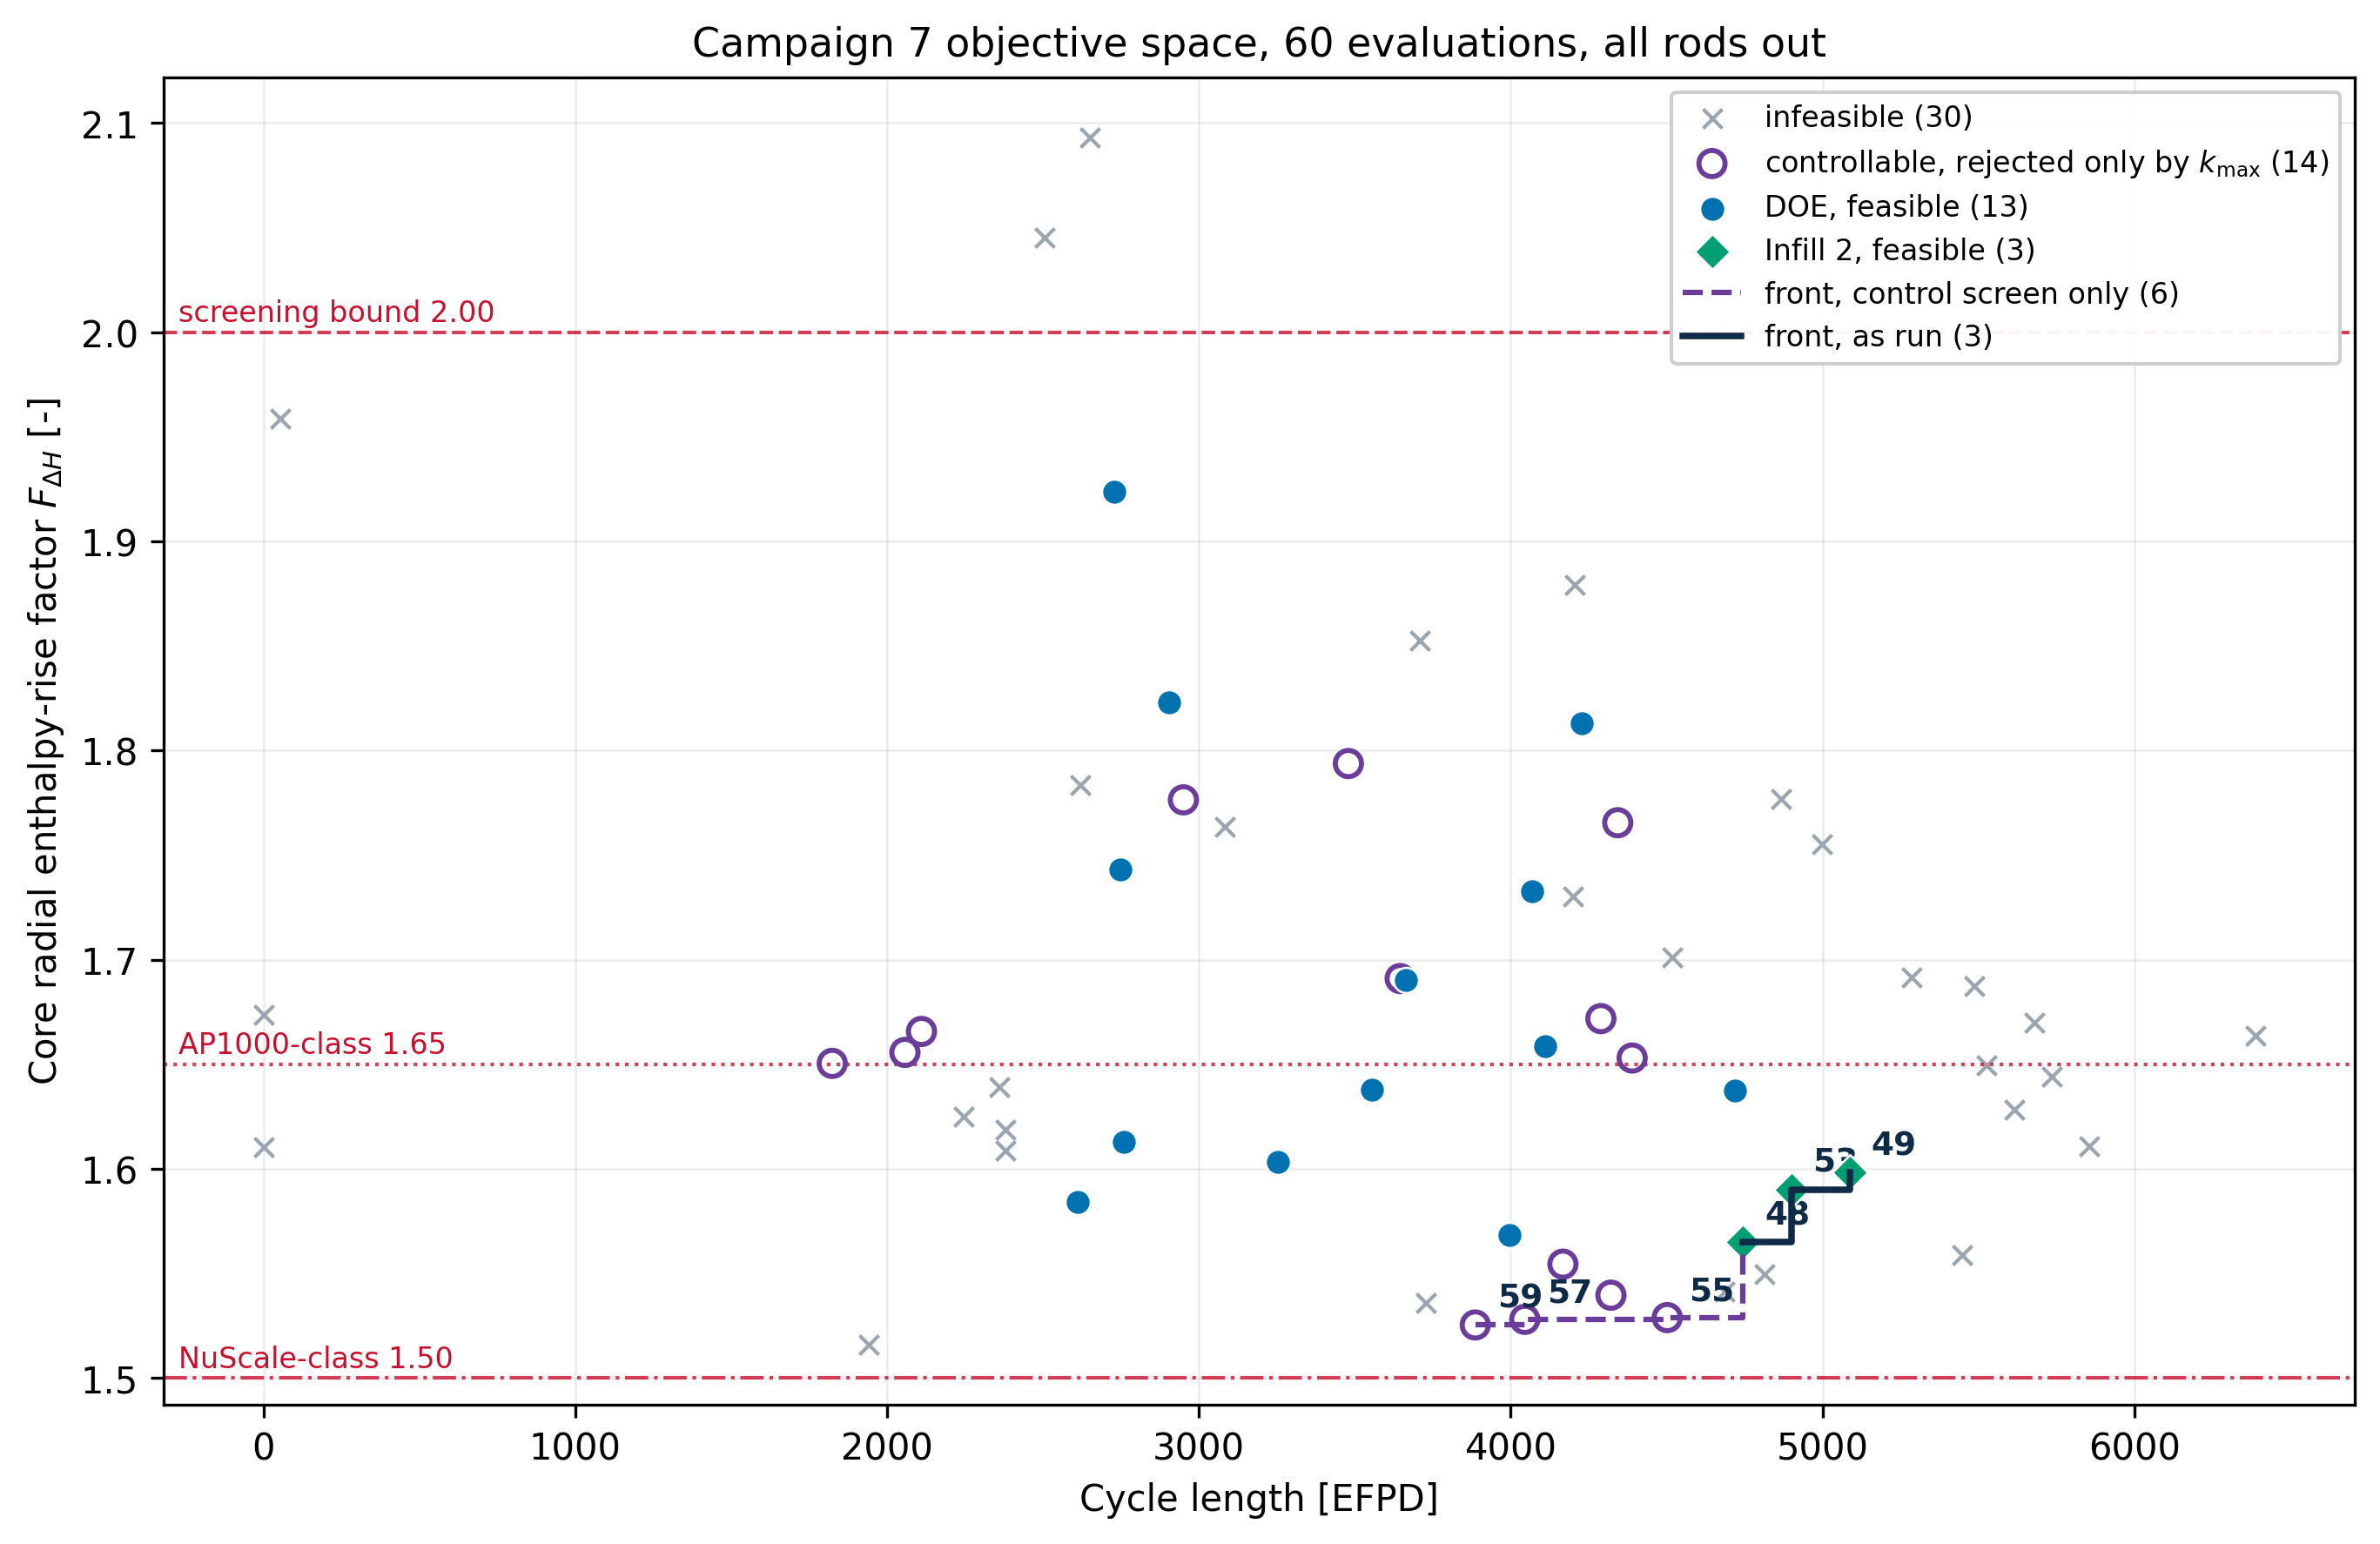
\includegraphics[width=\linewidth]{images/c7_pareto_60}
  \caption{Campaign 7 objective space with all rods out.}
  \label{fig:c7-pareto}
\end{figure}

Two properties of the front as run deserve stating. Its three designs
sit \num{240} to \SI{680}{pcm} below the ceiling, so the front is a
constraint boundary and not an interior trade. And the cycle lengths
are not comparable with Campaign 6, because the enrichment box is a
different one, and the longest feasible cycle of 5087 EFPD says nothing
about the reactor class that the 9981 EFPD of Campaign 6 did not
already say.

%% AUTHOR: one paragraph on why the low-peaking end of the control-screen
%% front lives at thick reflectors and narrow pitch, and on the physical
%% meaning of a front that doubles when a surrogate bound is removed.

\subsection{Regulating-bank worth and the reason the screens nest}
\label{sec:res-c7-worth}

The worth of the sixteen regulating banks is defined on the two core
solves of every evaluation.

\begin{equation}
\rho_\mathrm{bank}(\mathbf{x}) = k_\mathrm{eff}^\mathrm{core}(\mathbf{x}) - k_\mathrm{RE}(\mathbf{x})
\label{eq:bank-worth}
\end{equation}

\noindent where the symbols have the following meaning.

\begin{itemize}
  \item $\rho_\mathrm{bank}$ is the bank worth in units of $k$,
        dimensionless, reported in pcm by multiplying by $10^5$.

  \item $k_\mathrm{eff}^\mathrm{core}$ is the unrodded core eigenvalue
        at beginning of life, dimensionless.

  \item $k_\mathrm{RE}$ is the eigenvalue with the sixteen
        regulating-bank assemblies inserted, dimensionless.
\end{itemize}

Across the archive the worth ranges from \num{10936} to
\SI{22699}{pcm} with a median of \SI{16510}{pcm}. Figure~\ref{fig:c7-worth}
shows its two strongest drivers, with least-squares trends drawn as
visual guides only, and Figure~\ref{fig:c7-influence} the rank
correlations of all six variables with the objectives, the worth and the
rodded peaking, over the whole archive and over the feasible subset.

\begin{figure}[htbp]
  \centering
  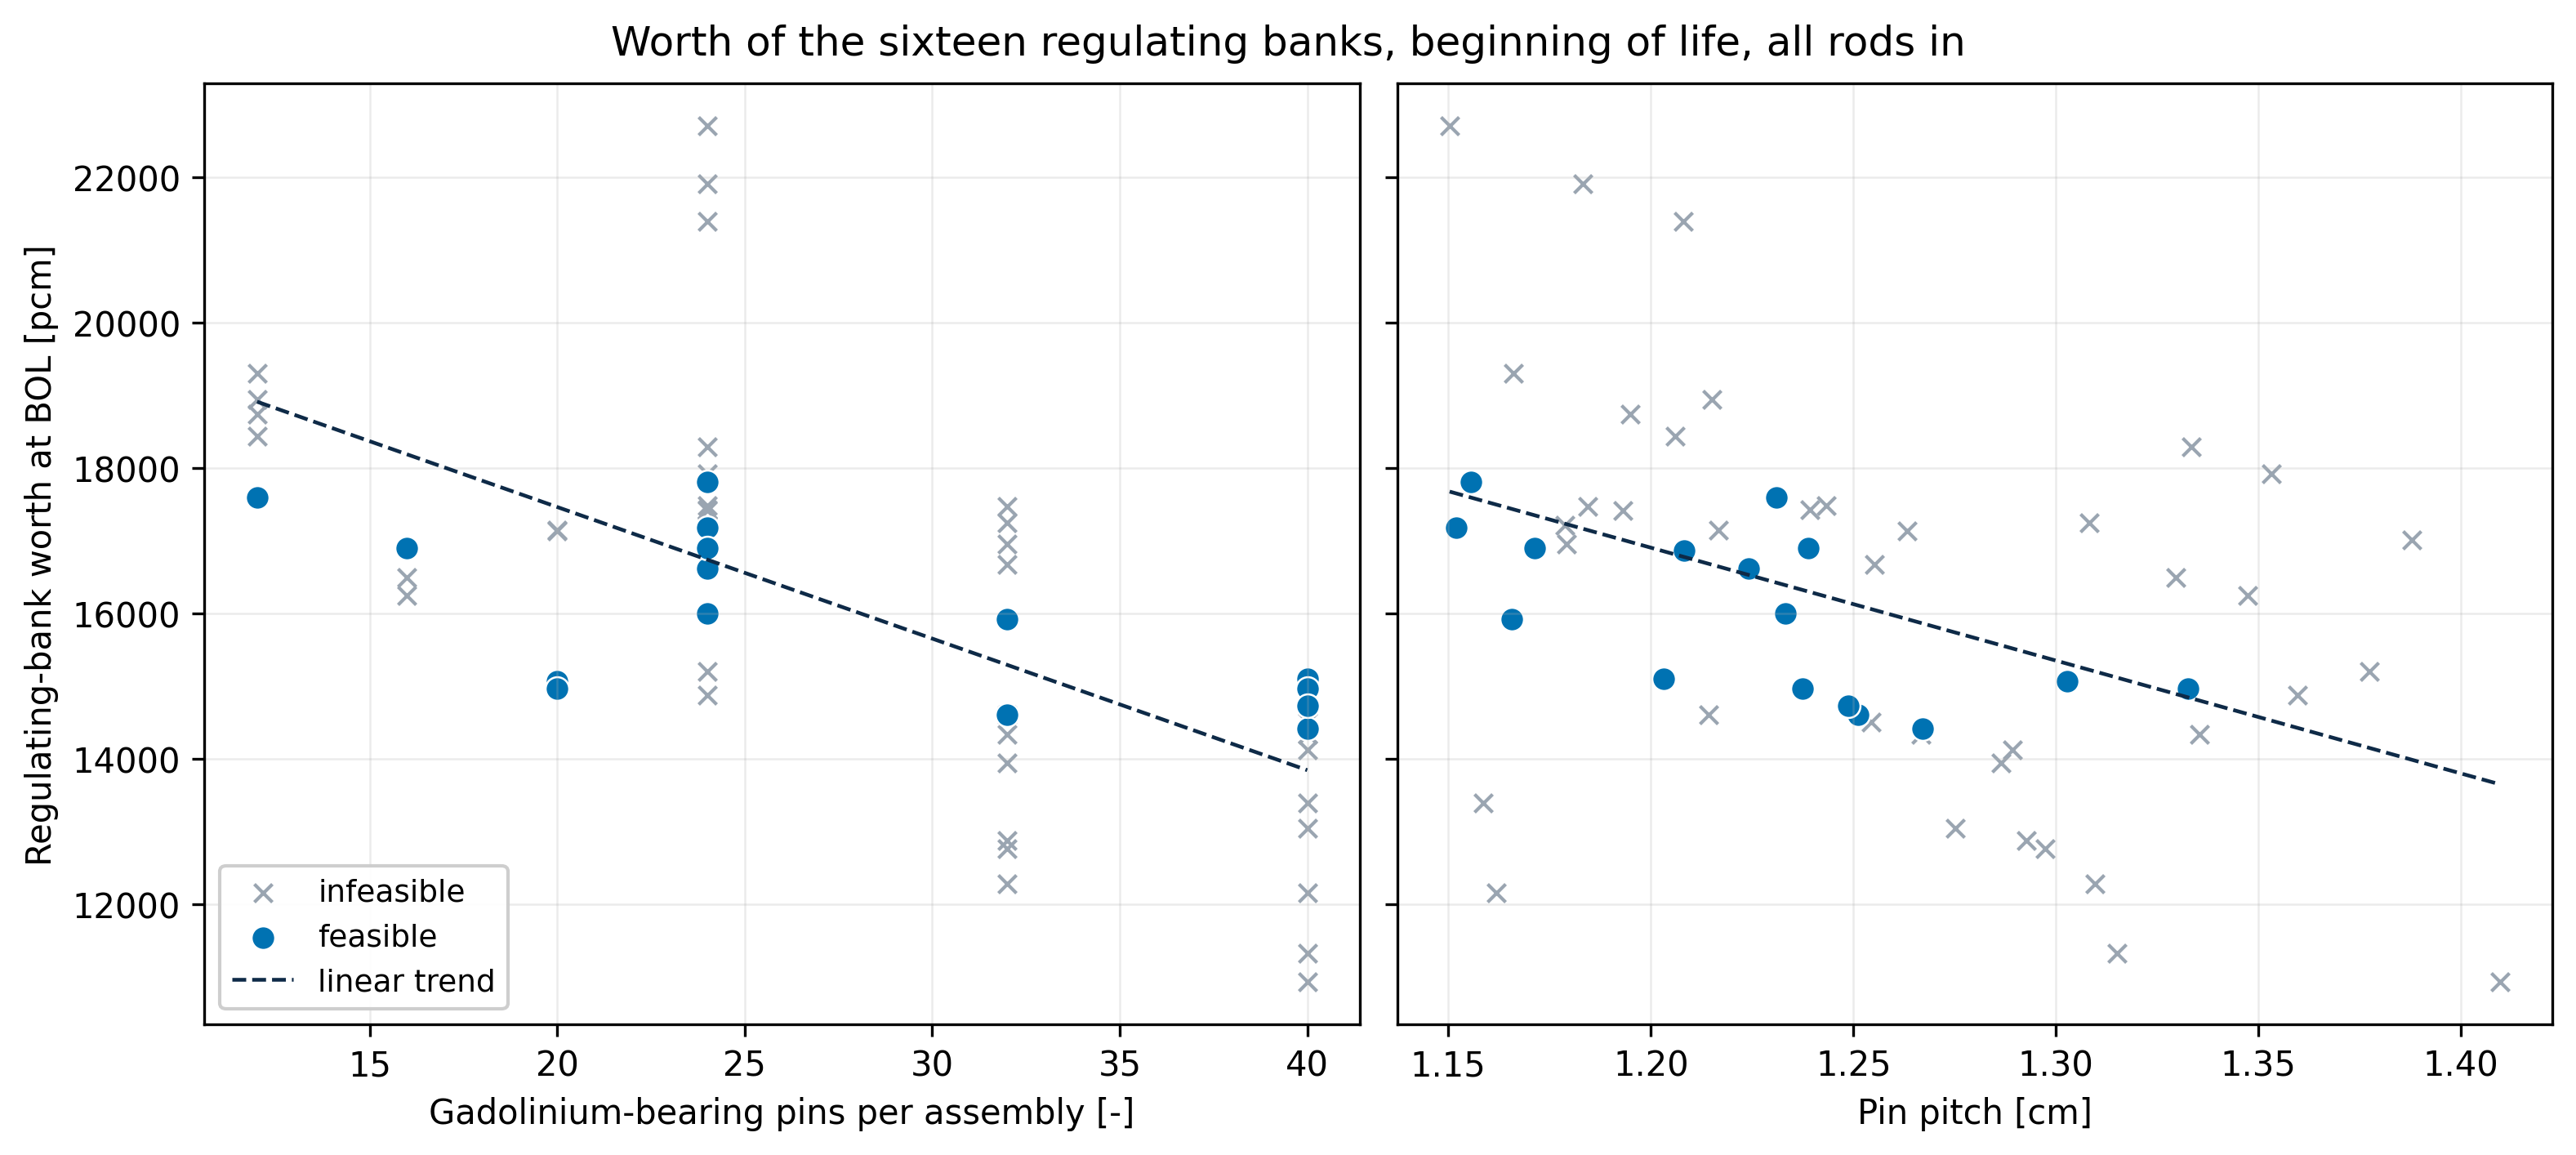
\includegraphics[width=\linewidth]{images/c7_rod_worth}
  \caption{Worth of the sixteen regulating banks against the gadolinium pin count and the pin pitch.}
  \label{fig:c7-worth}
\end{figure}

\begin{figure}[htbp]
  \centering
  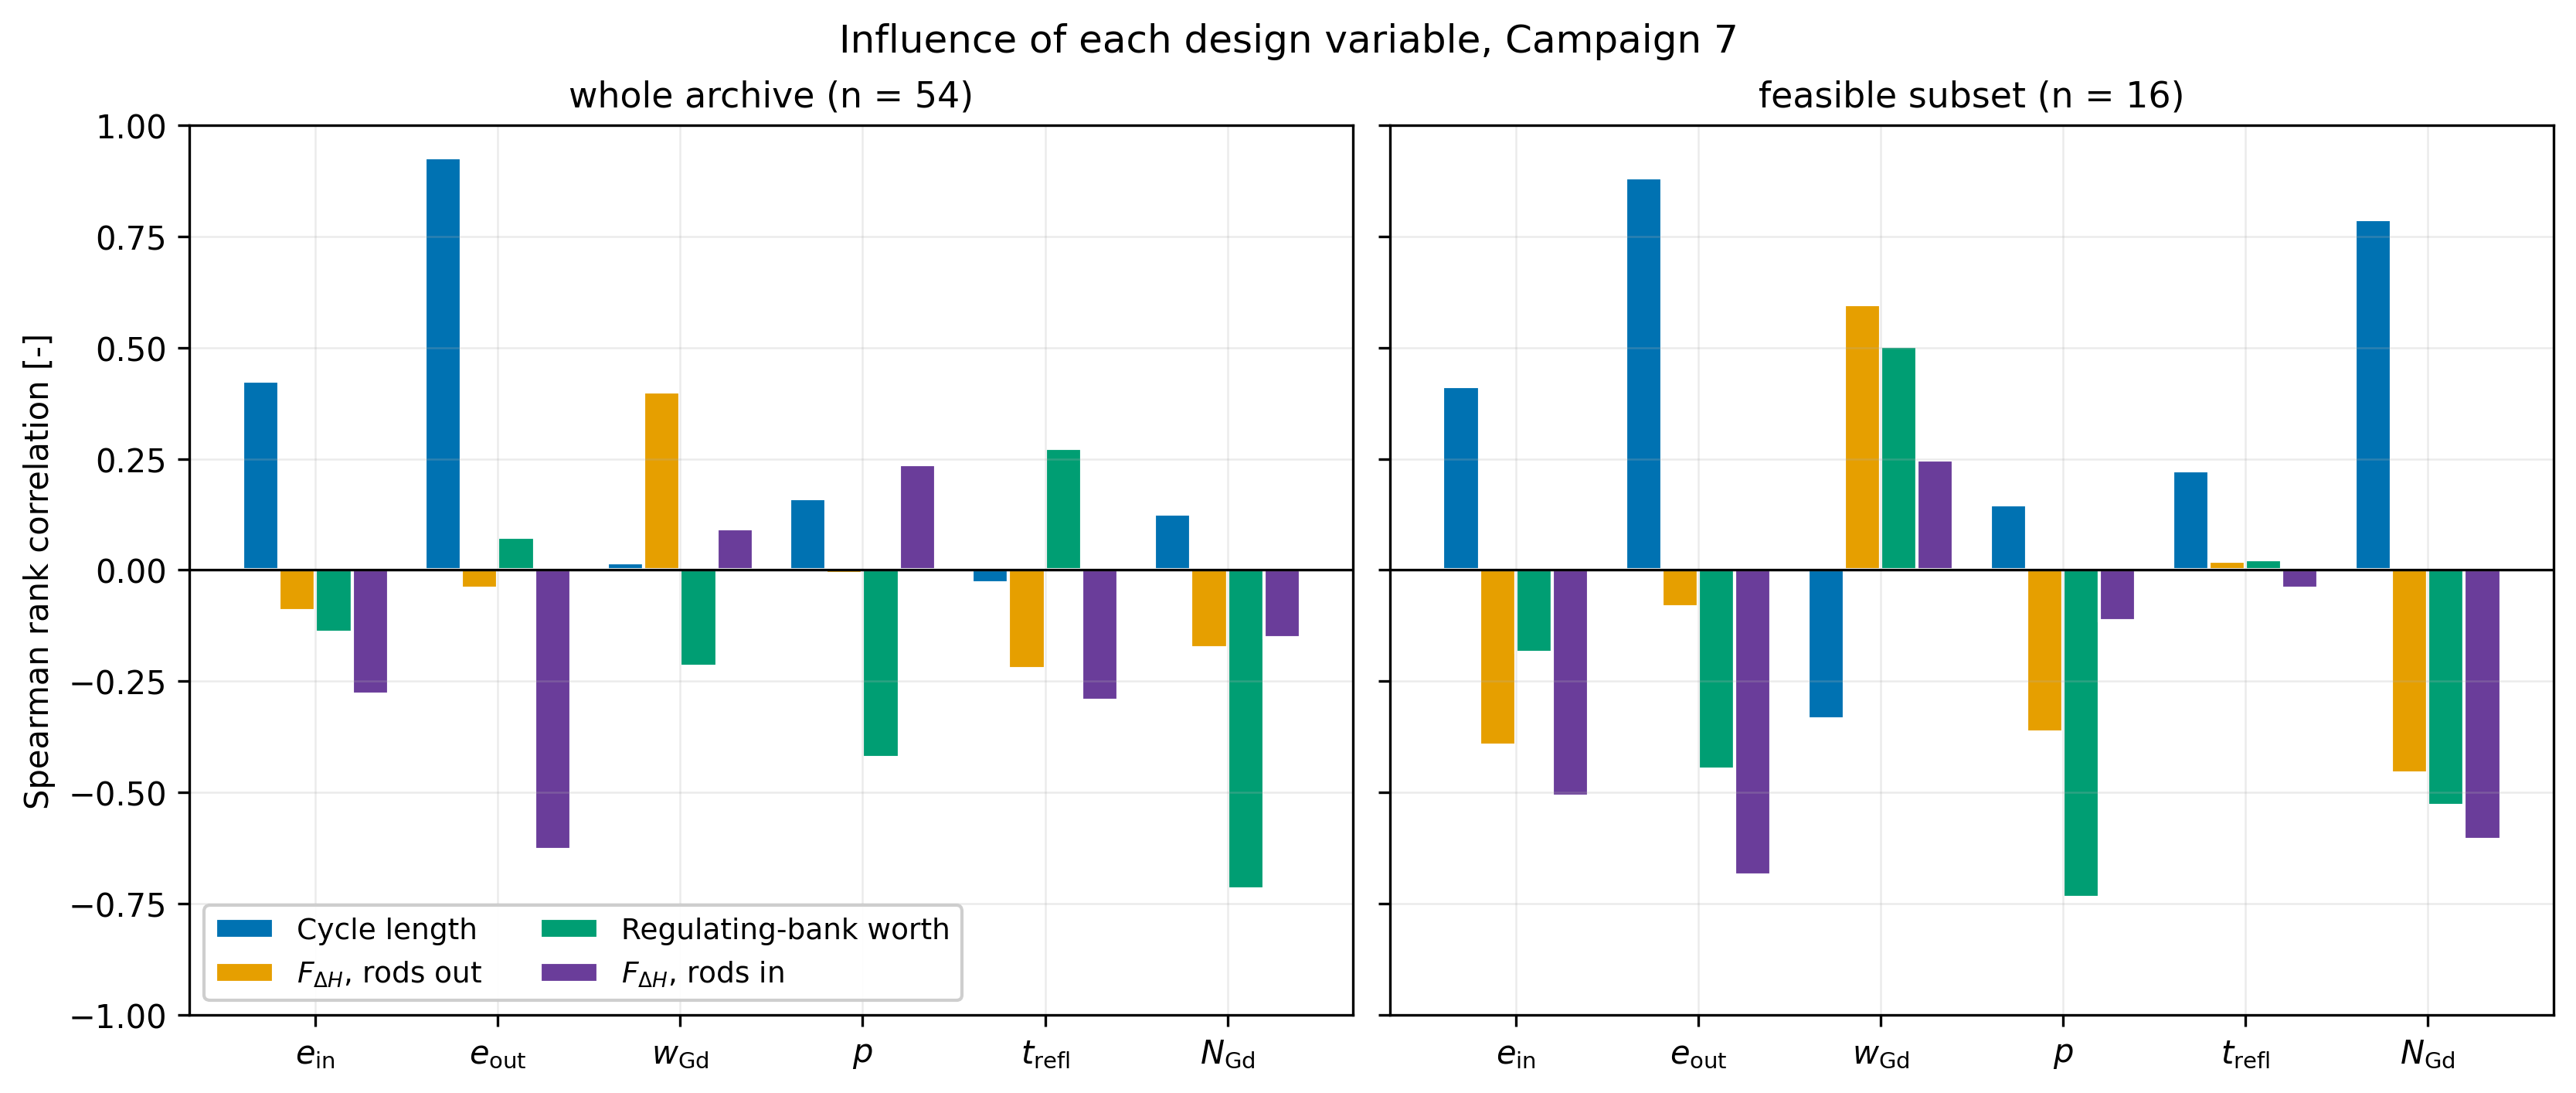
\includegraphics[width=\linewidth]{images/c7_vars_influence}
  \caption{Campaign 7: Spearman rank correlation of each design variable with the objectives, the regulating-bank worth and the rodded peaking.}
  \label{fig:c7-influence}
\end{figure}

The worth correlates at $-0.68$ with the gadolinium pin count, at
$-0.45$ with the pitch and at $+0.61$ with the unrodded eigenvalue.
Gadolinium depresses the eigenvalue and the bank worth together, so the
designs with the least worth are the heavily poisoned ones, which are
already far below the ceiling for a different reason. That is why the
two screens nest in this design space, and it is also why the
eight-design derivation of the ceiling looked safe when it was not.
The eight designs were all high-enrichment, forty-pin designs from one
corner of the Campaign 6 front, and their worths were alike because
their poison inventories were alike.

The measurement also settles a question left open since Campaign 4.
The ceiling of 1.35 used in Campaigns 1 to 6 was described as a
screening value not traceable to a primary source. Deriving the
ceiling from the worth of all seven banks, that is all 32 control rod
assemblies, with the same \SI{1000}{pcm} margin gives 1.368. The value
used through six campaigns sits two per cent below the measured
all-bank controllability bound of this core. It is a measured quantity
in retrospect, and the methodology chapter now states it as such,
with the caveat that an all-bank insertion with a \SI{1000}{pcm}
operating margin is not a licensing shutdown margin, which also
requires the highest-worth assembly stuck out and the cold, xenon-free
state.

\subsection{Peaking with the regulating banks inserted}
\label{sec:res-c7-rodded}

The peaking objective is evaluated with all rods out. The same core
solve that measures $k_\mathrm{RE}$ also yields the radial peaking
with the sixteen banks inserted, and Figure~\ref{fig:c7-rodded} plots
the two against each other. Every design lies above the screening bound
of 2.0 in the rodded configuration.

\begin{figure}[htbp]
  \centering
  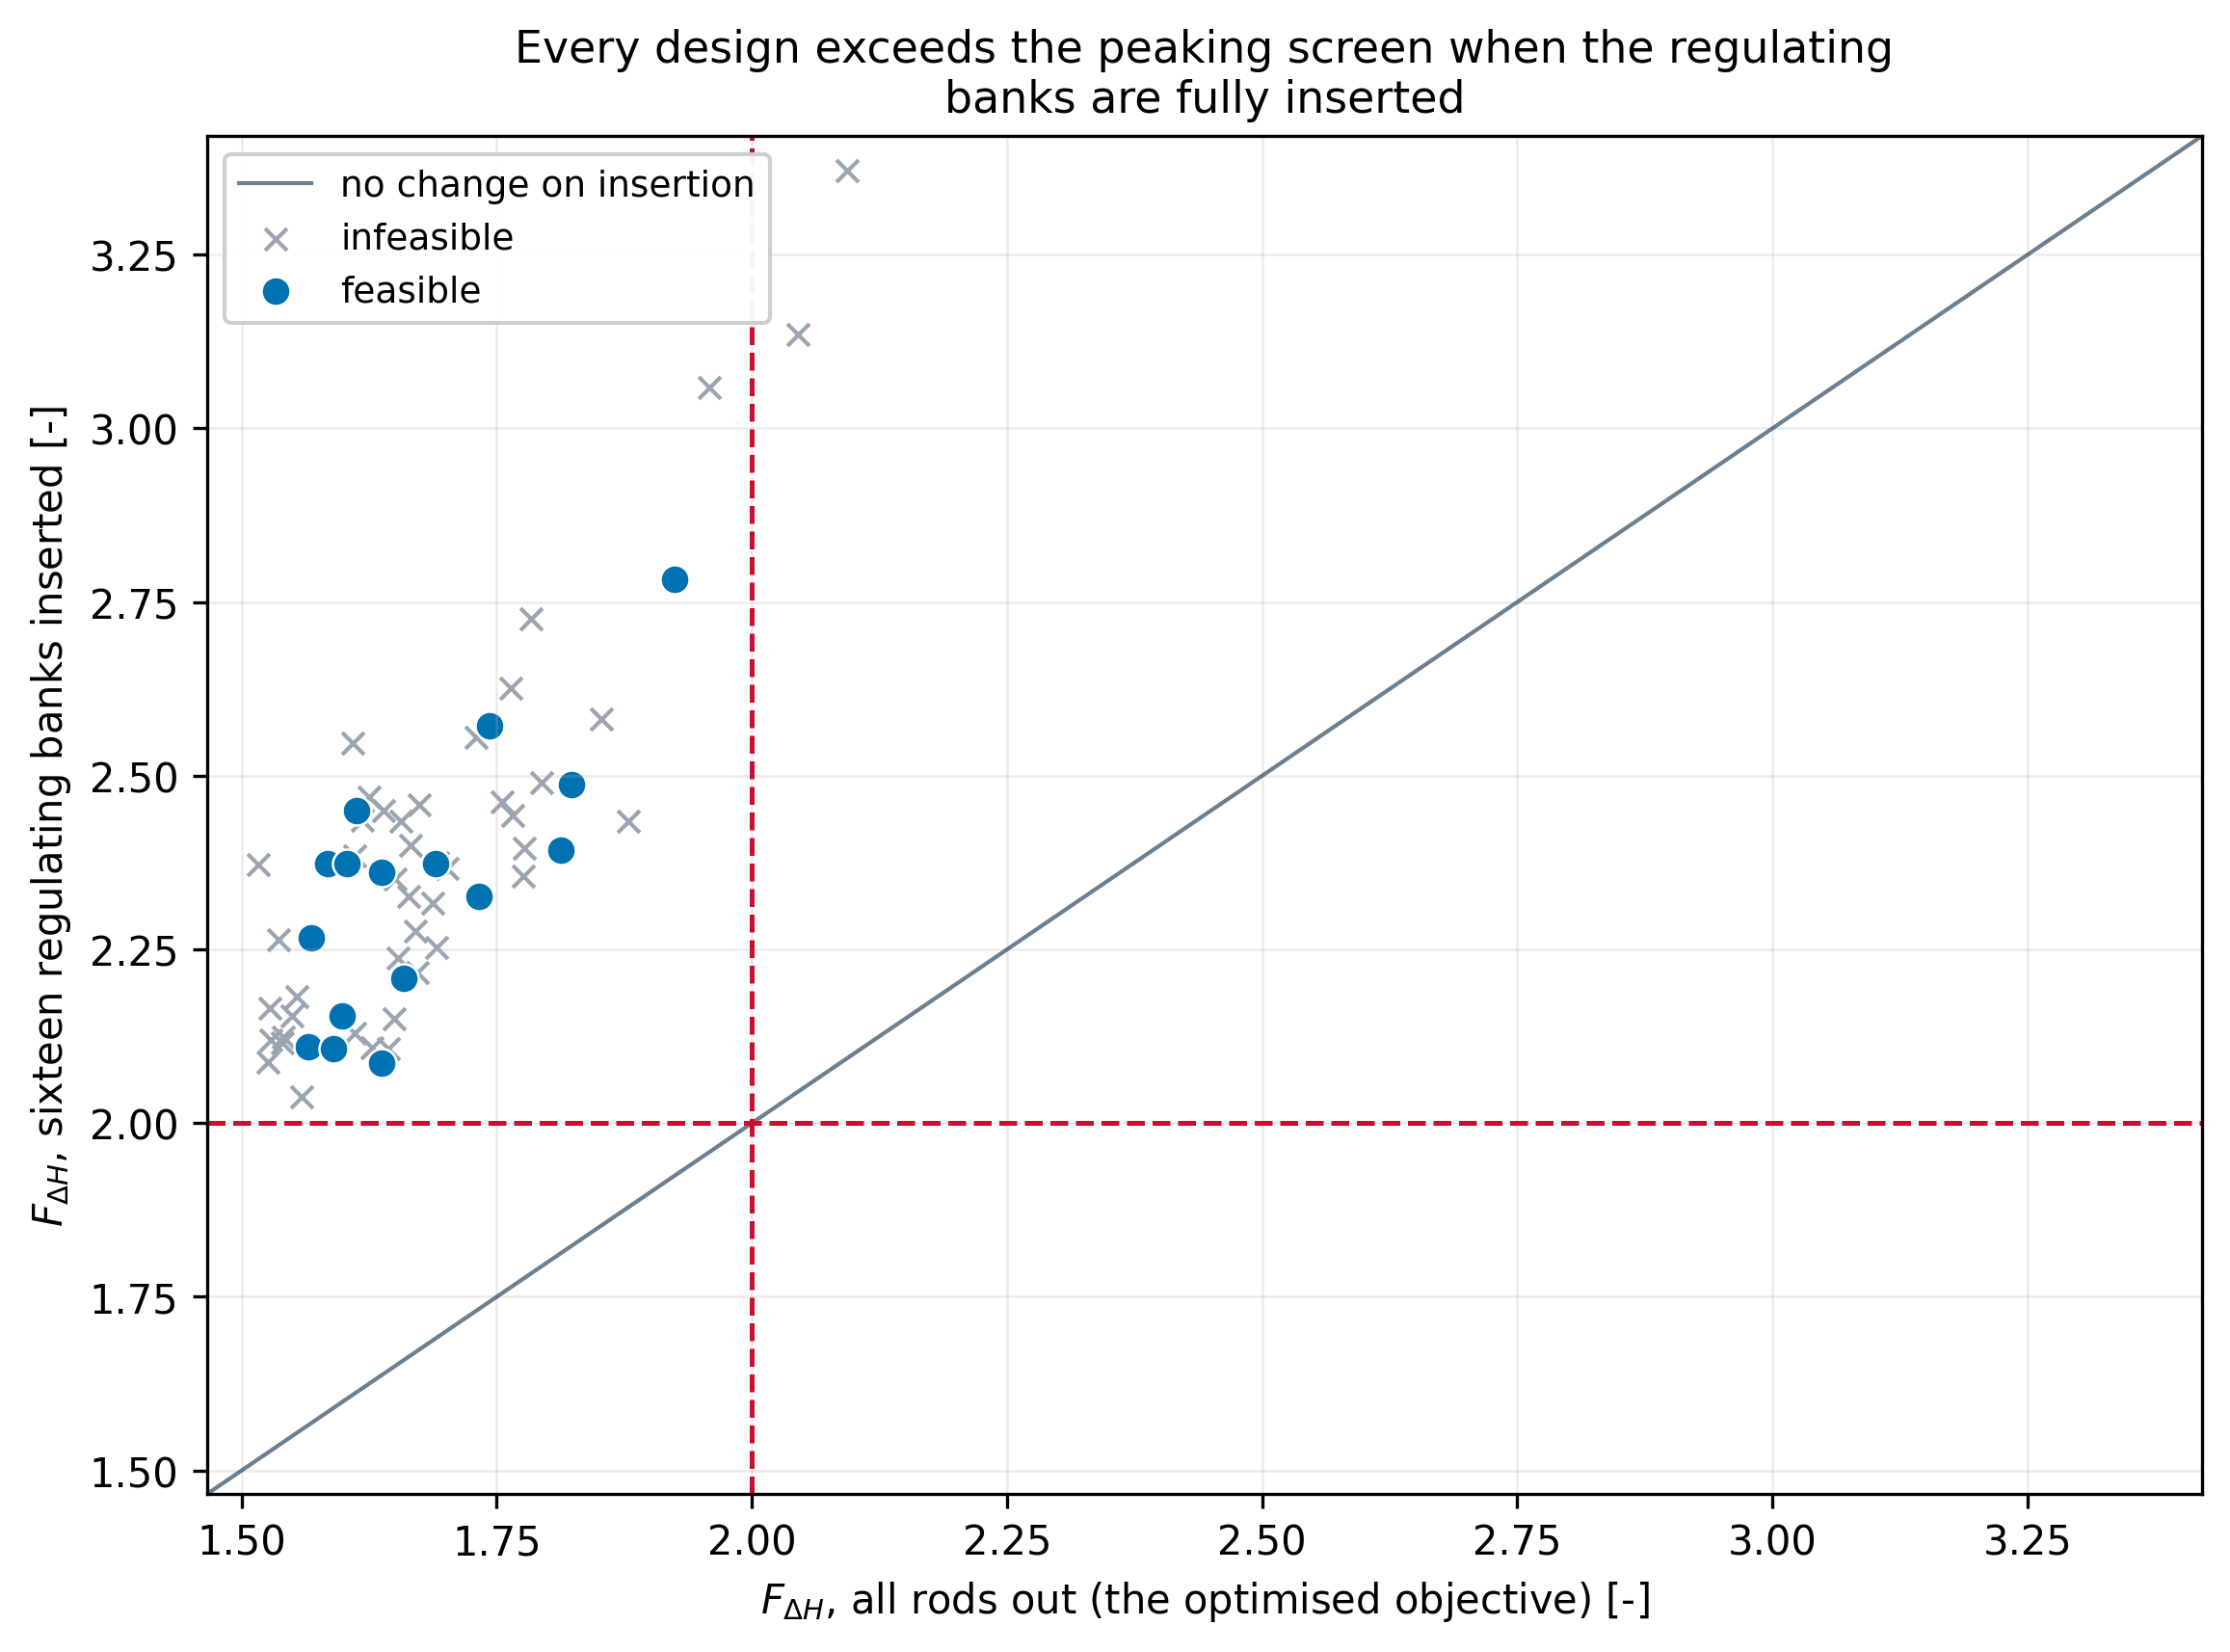
\includegraphics[width=0.85\linewidth]{images/c7_rodded_peaking}
  \caption{Campaign 7 radial peaking with all rods out against the same quantity with the sixteen regulating banks inserted.}
  \label{fig:c7-rodded}
\end{figure}

With the banks inserted $F_{\Delta H}$ runs from 2.038 to 3.371 with a
mean of 2.375, against 1.516 to 2.093 unrodded. The insertion penalty
ranges from 0.449 to 1.278 and is design dependent, correlating at
$-0.81$ with the outer-zone enrichment over the archive. Every one of
the 60 designs exceeds the screening bound of 2.0 in the rodded
configuration, and the three front designs sit between 2.11 and 2.16.

Two framings are required and neither should be overstated. Sixteen
banks fully inserted is the extreme of the regulating band used here as
a controllability test, not an operating configuration, so the rodded
value is an upper bound on operating peaking rather than an operating
value. Even so, the objective being minimised moves by half a unit or
more when the rods go in, and it moves by a design-dependent amount.
A design selected for low unrodded peaking is not thereby a design
with low rodded peaking. This is recorded as a limitation of the
objective set and as the motivation for the two-level reading of
Campaign 8.

%% AUTHOR: physical interpretation of the negative correlation between
%% the insertion penalty and the outer-zone enrichment.

\subsection{Depletion histories and the statistical error on the cycle length}
\label{sec:res-c7-uncertainty}

The assembly depletion solves are the only transport runs whose output
reaches the campaign log, and the log therefore holds the complete
$k_\infty(B)$ history of every design. Figure~\ref{fig:c7-histories}
reconstructs all 60 histories with the end-of-cycle crossing of the
leakage-corrected target marked in red, feasible designs on the left.
The gadolinium burnout maximum is visible between \num{7.5} and
\SI{17.5}{MWd/kgHM}, and no design approaches the \SI{75}{MWd/kgHM}
screen.

\begin{figure}[htbp]
  \centering
  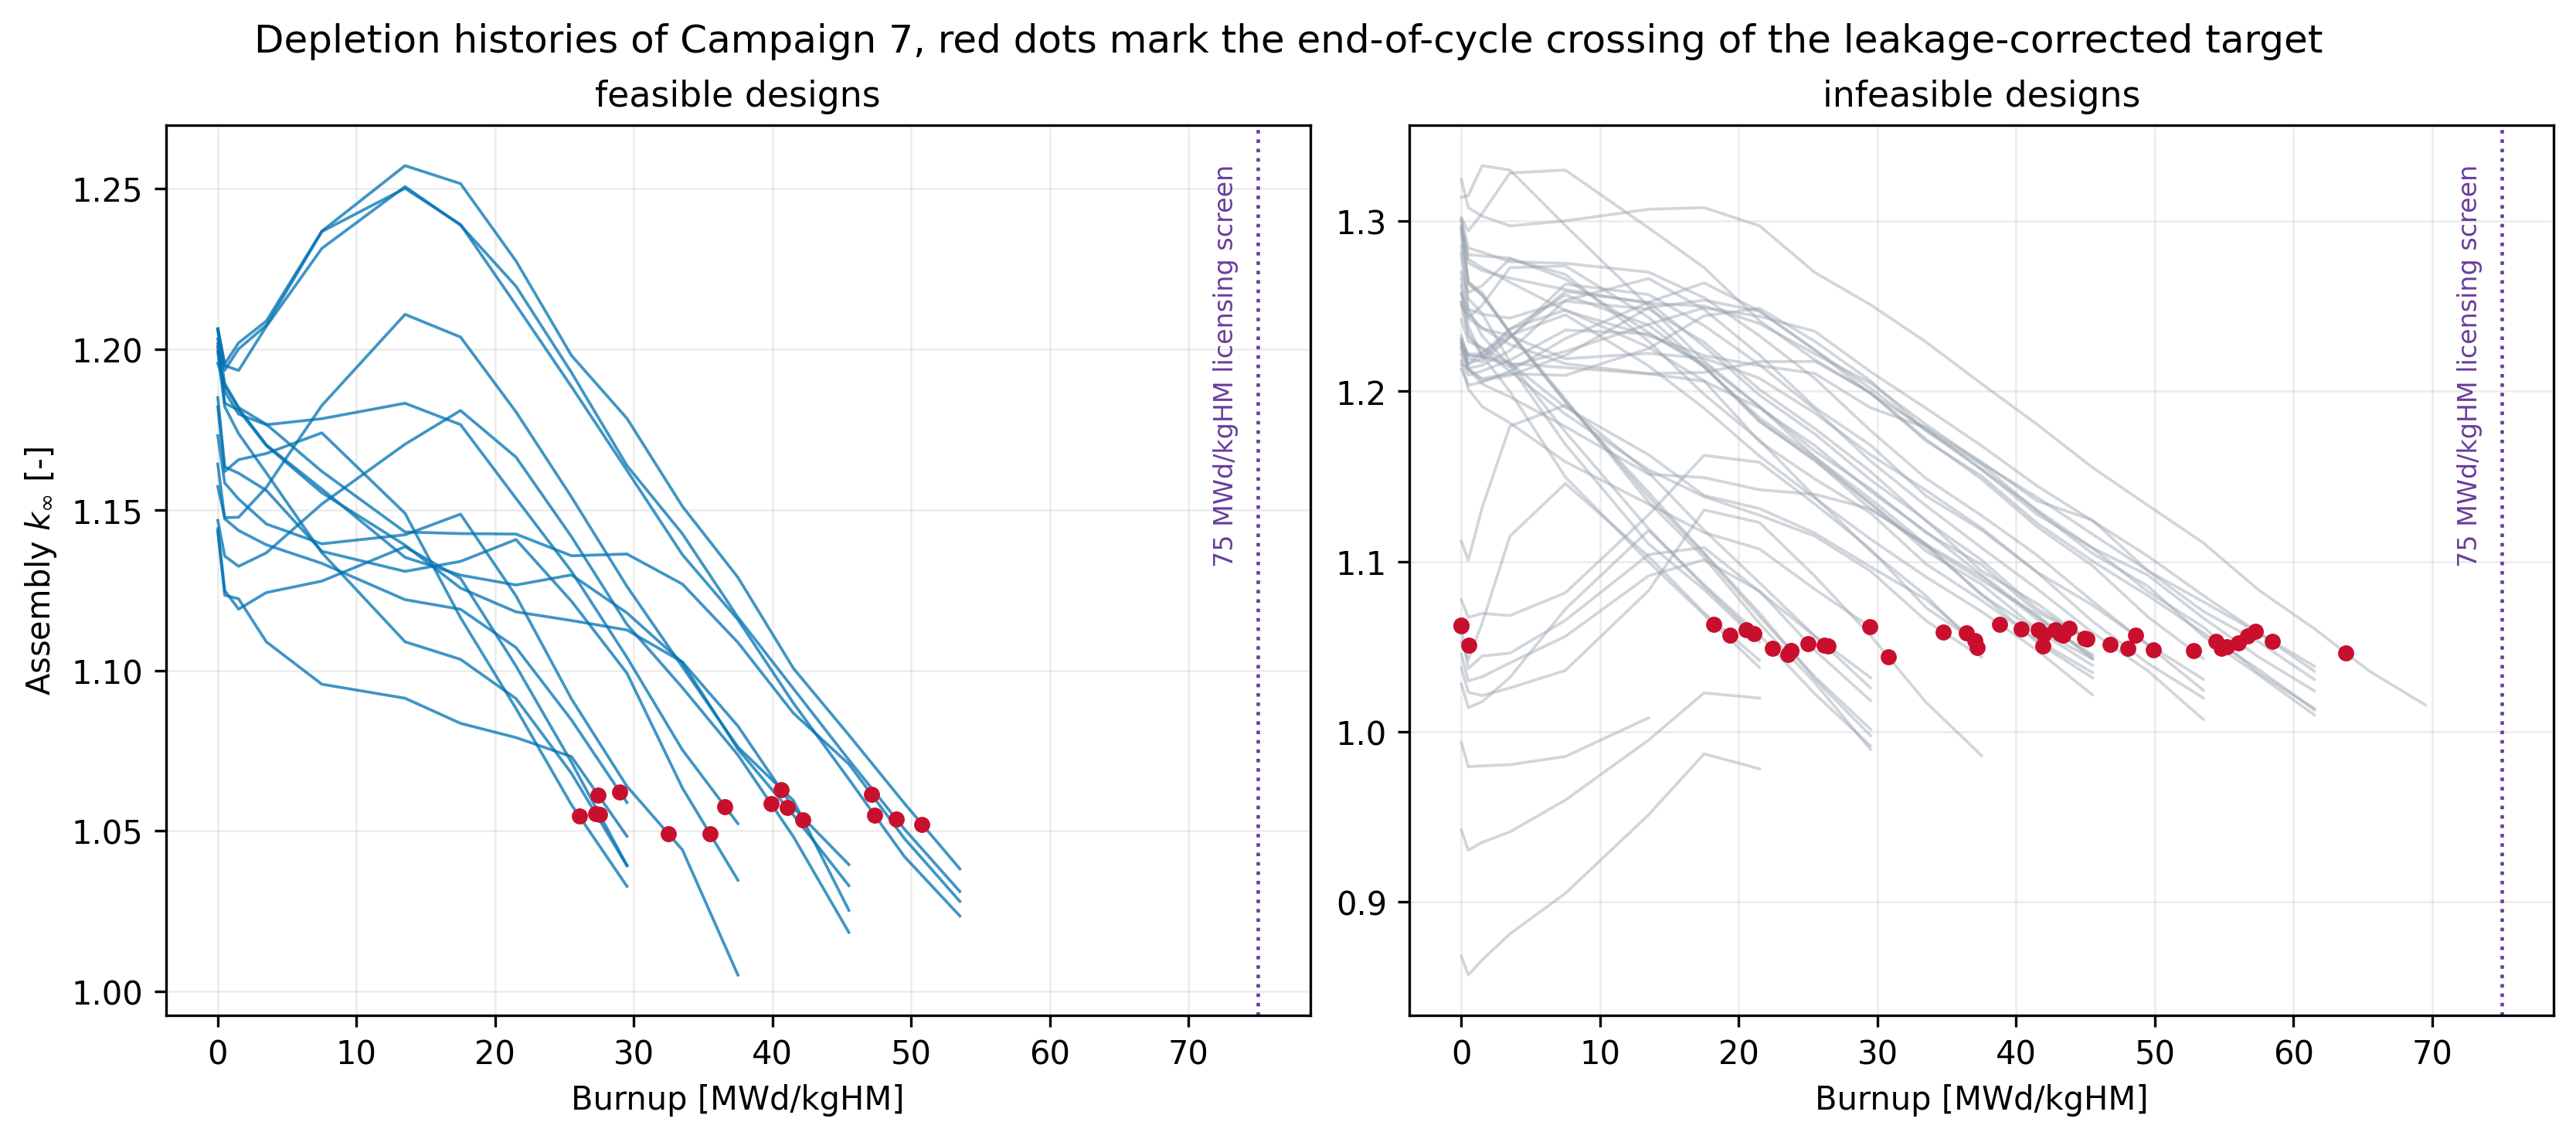
\includegraphics[width=\linewidth]{images/c7_kinf_histories}
  \caption{Assembly infinite multiplication factor against burnup for every Campaign 7 design.}
  \label{fig:c7-histories}
\end{figure}

The reconstruction was validated against the archive. Taking the last
descending crossing of the target reproduces the stored end-of-cycle
burnup of all 57 crossing designs to within \SI{0.0011}{MWd/kgHM}. The
last crossing is the correct rule because the gadolinium burnout makes
the early history non-monotonic. The three designs without a crossing
are the two subcritical cores at zero cycle length and one design
ending at 55 EFPD.

Three facts follow from the figure. The gadolinium hump raises
$k_\infty$ by up to \num{0.119} before the decline, measured in
Section~\ref{sec:res-c7-hump}. The highest end-of-cycle
burnup in the campaign is \SI{63.8}{MWd/kgHM}, so the
\SI{75}{MWd/kgHM} discharge screen of Section~\ref{sec:meth-atf} is
inactive and no design is censored, unlike Campaign 6. And the local
slope at end of cycle is steep, which governs the statistical error on
the cycle length.

The Monte Carlo error on the cycle length is obtained by propagating
the uncertainties of the two transport states that bracket the
crossing.

\begin{equation}
\sigma_B^2 = \left(\frac{\Delta B\,(k_\mathrm{t} - k_{j+1})}{(k_j - k_{j+1})^2}\right)^2 \sigma_{k_j}^2
+ \left(\frac{\Delta B\,(k_j - k_\mathrm{t})}{(k_j - k_{j+1})^2}\right)^2 \sigma_{k_{j+1}}^2
\label{eq:sigma-beoc}
\end{equation}

\noindent where the symbols have the following meaning.

\begin{itemize}
  \item $\sigma_B$ is the statistical uncertainty of the end-of-cycle
        burnup, in MWd/kgHM.

  \item $\Delta B$ is the burnup step between the two bracketing
        states, in MWd/kgHM.

  \item $k_j$ and $k_{j+1}$ are the infinite multiplication factors at
        the states before and after the crossing, dimensionless.

  \item $k_\mathrm{t}$ is the leakage-corrected target, dimensionless,
        treated as exact.

  \item $\sigma_{k_j}$ and $\sigma_{k_{j+1}}$ are the reported Monte
        Carlo standard deviations of the two states, dimensionless.
\end{itemize}

The cycle length follows from the specific power.

\begin{equation}
\sigma_\mathrm{EFPD} = \frac{1000\,\sigma_B}{P_\mathrm{sp}}
\label{eq:sigma-efpd}
\end{equation}

\noindent where the symbols have the following meaning.

\begin{itemize}
  \item $\sigma_\mathrm{EFPD}$ is the statistical uncertainty of the
        cycle length, in effective full power days.

  \item $P_\mathrm{sp}$ is the specific power of the core,
        \SI{9.98}{W/gHM}.
\end{itemize}

Figure~\ref{fig:c7-uncertainty} plots the propagated error against the
cycle length and against the reactivity slope at end of cycle. The error
is set by the slope at end of cycle, and the length of the cycle does
not govern it.

\begin{figure}[htbp]
  \centering
  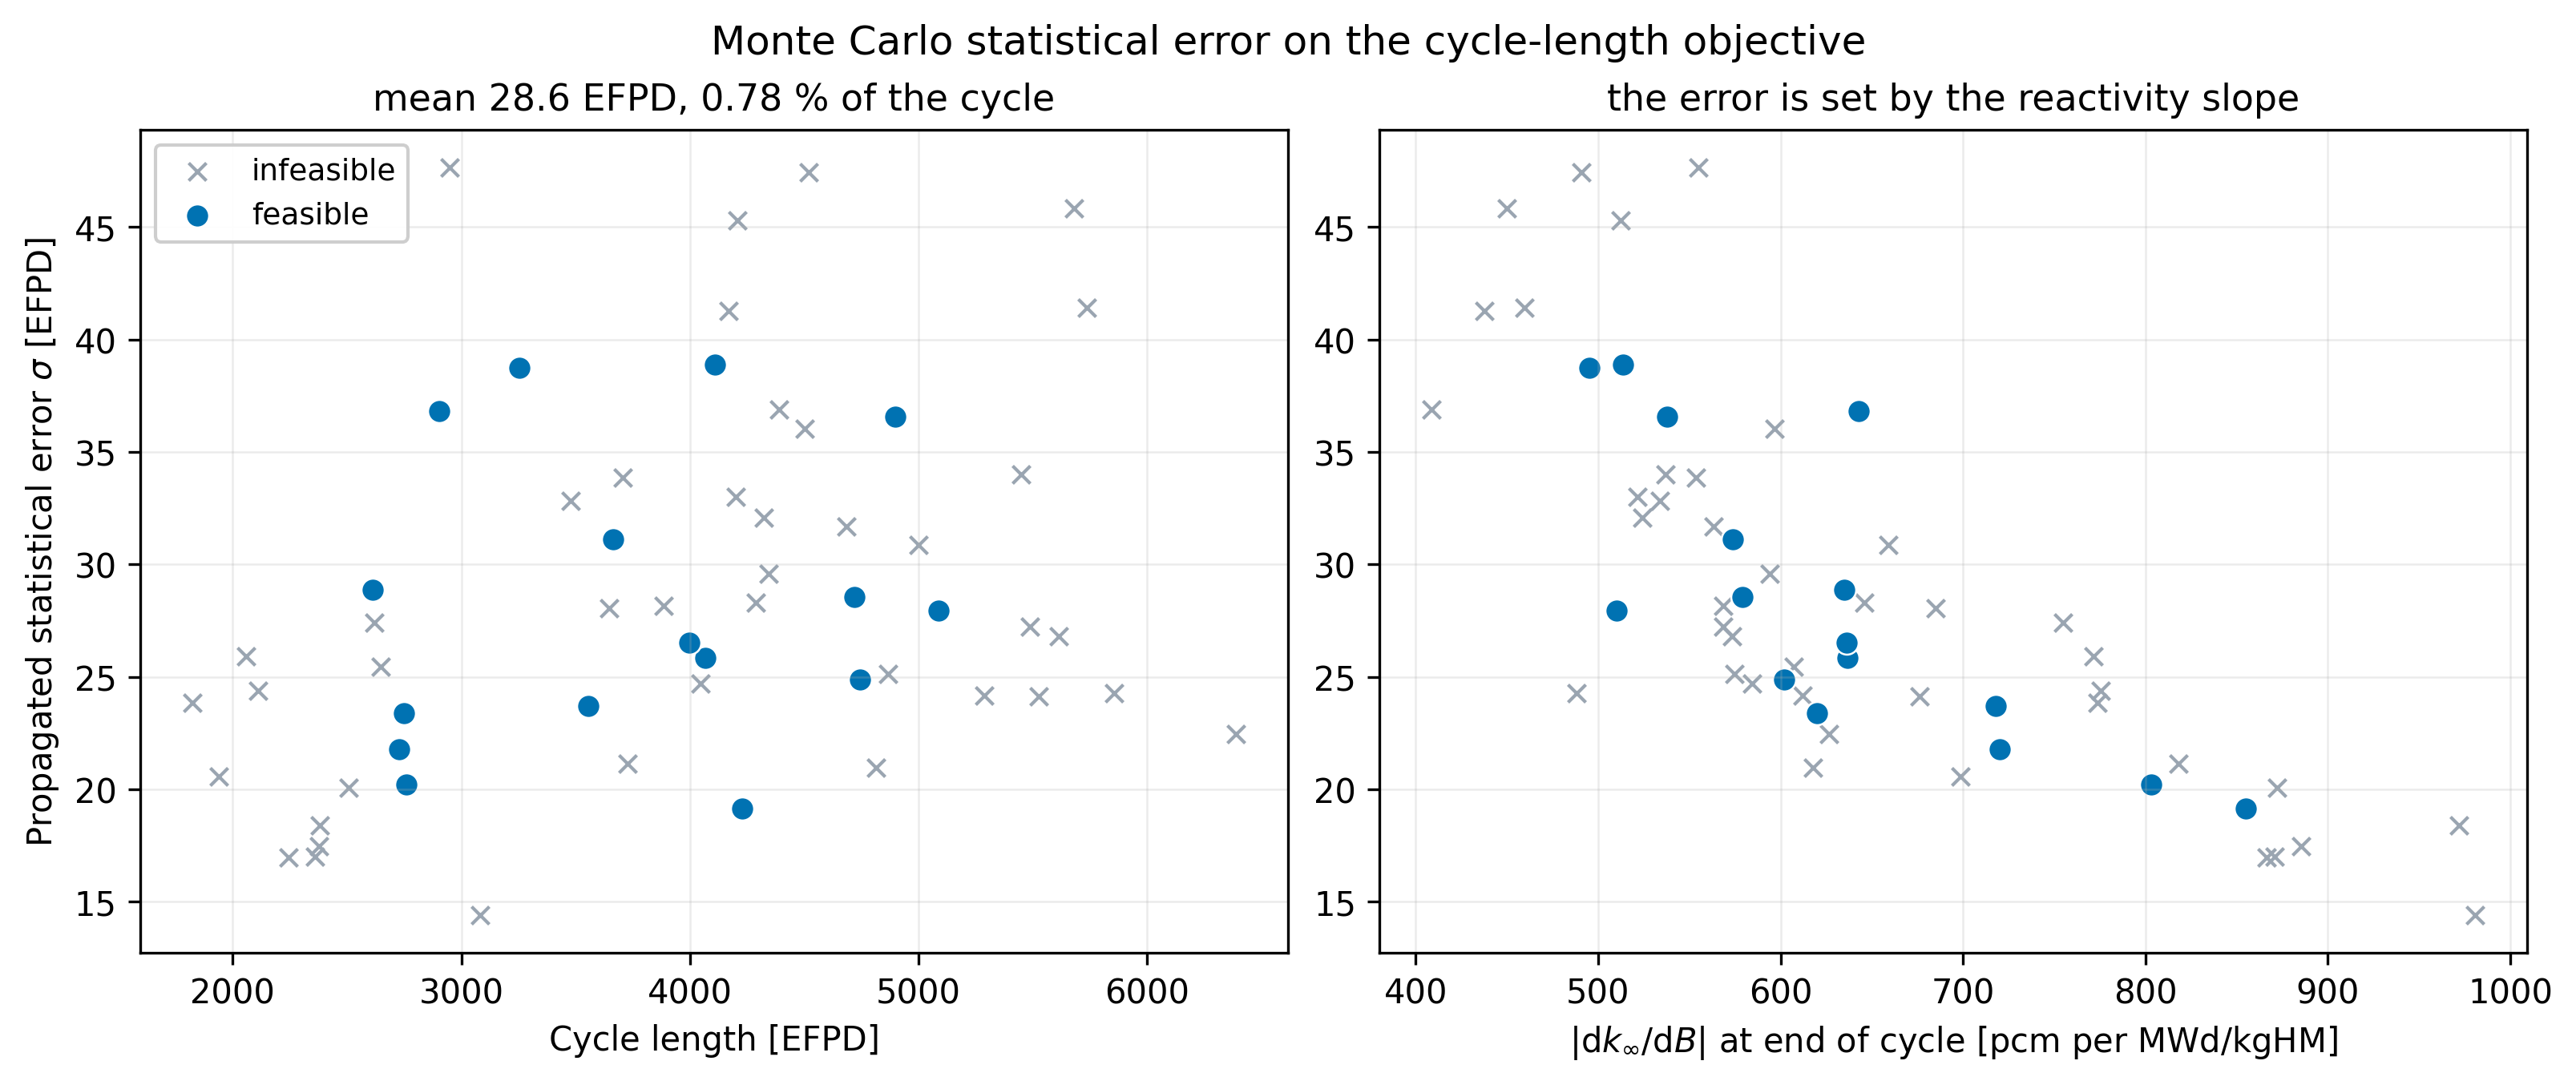
\includegraphics[width=\linewidth]{images/c7_cycle_uncertainty}
  \caption{Propagated Monte Carlo error on the Campaign 7 cycle length.}
  \label{fig:c7-uncertainty}
\end{figure}

Table~\ref{tab:c7-uncertainty} summarises the result and
Figure~\ref{fig:c7-uncertainty} shows it. The slope at end of cycle
lies between 409 and \SI{981}{pcm} per MWd/kgHM with a median of 607.
The resulting error has a mean of 28.6 EFPD, \SI{0.78}{\%} of the
cycle, and a worst case of 47.7 EFPD, \SI{1.62}{\%}. On the six front
designs it is 25 to 37 EFPD. The smallest gap between adjacent front
designs is 154 EFPD, about five standard deviations, so the ordering of
the front in cycle length is statistically resolved.

\begin{table}[htbp]
  \centering
  \caption{Statistical error on the cycle length over the 57 designs
  with a resolved end-of-cycle crossing.}
  \label{tab:c7-uncertainty}
  \begin{tabular}{lccc}
    \toprule
    Quantity & Minimum & Median & Maximum \\
    \midrule
    Slope at end of cycle [pcm per MWd/kgHM] & 409 & 607 & 981 \\
    Bracketing sigma on $k_\infty$ [pcm]     & 178 & 218 & 274 \\
    $\sigma_\mathrm{EFPD}$ [d]               & 14.4 & 27.2 & 47.7 \\
    $\sigma_\mathrm{EFPD}$ as a fraction of the cycle [\%] & 0.35 & 0.74 & 1.62 \\
    \bottomrule
  \end{tabular}
\end{table}

The peaking axis is the opposite case. The front designs are separated
by 0.003 to 0.036 in $F_{\Delta H}$, the entropy study of
Section~\ref{sec:res-c6} bounded the systematic shift at $\pm 0.02$,
and no statistical error on the core peaking tally has been measured.
The ordering of the front in peaking is therefore not resolved, and
designs 59, 57 and 55 at 1.525, 1.528 and 1.529 must be treated as
indistinguishable until the tally errors are read from the statepoints.

\openpoint{Measure $\sigma(F_{\Delta H})$ from the per-bin relative
errors of the core mesh tally on the six front designs, or by seed
replicates, before any ordering claim on the peaking axis is made.}

\subsection{The gadolinium hump in the Campaign 7 archive}
\label{sec:res-c7-hump}

The histories of Section~\ref{sec:res-c7-uncertainty} carry a second
measurement that the crossing analysis does not use. Between beginning
of life and the end-of-cycle decline, the assembly eigenvalue of a
gadolinia-bearing design first rises, because the poison burns out
faster than the fuel. The maximum of that rise, and not the beginning
of life, is the most reactive state the core ever occupies. Any
reactivity screen written at beginning of life therefore screens the
wrong state whenever a hump is present.

The hump is defined on the reactivity scale.

\begin{equation}
  \Delta\rho_\mathrm{hump} = \rho\!\left(k_\mathrm{peak}\right) -
  \rho\!\left(k_\mathrm{BOL}\right),
  \qquad
  \rho(k) = 10^{5}\,\frac{k-1}{k}
  \label{eq:c7-hump}
\end{equation}

where the symbols have the following meaning.

\begin{itemize}
  \item $\Delta\rho_\mathrm{hump}$ is the reactivity gained between
        beginning of life and the operating maximum, in pcm.
  \item $k_\mathrm{BOL}$ is the assembly infinite multiplication factor
        at zero burnup, xenon-free, at \SI{1000}{ppm} soluble boron,
        dimensionless.
  \item $k_\mathrm{peak}$ is the maximum of the assembly infinite
        multiplication factor over the operating points, dimensionless.
  \item $\rho$ is the reactivity, in pcm.
\end{itemize}

Figure~\ref{fig:c7-khist-gd} shows the same histories as
Figure~\ref{fig:c7-histories}, coloured by gadolinia weight fraction
instead of by feasibility, and Table~\ref{tab:c7-hump} lists the
fifteen designs with the largest humps.

\begin{figure}[htbp]
  \centering
  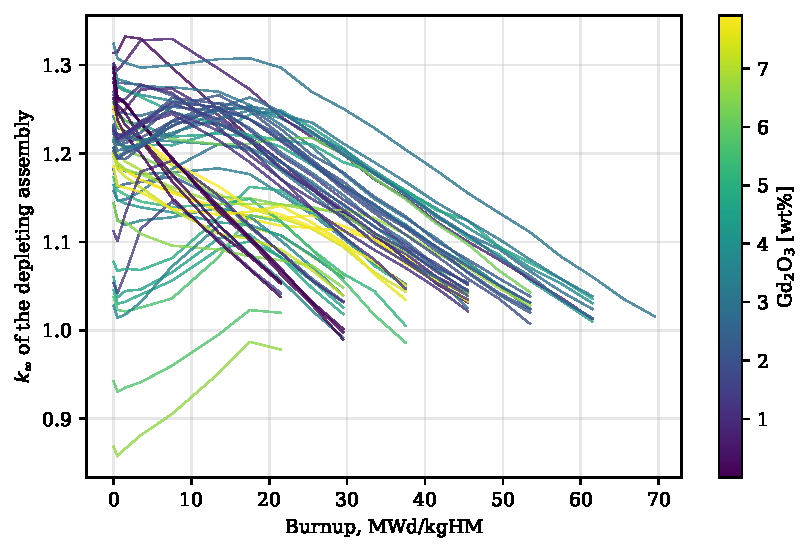
\includegraphics[width=0.95\linewidth]{images/k_histories}
  \caption[Campaign 7 histories coloured by gadolinia loading]{Assembly
  infinite multiplication factor against burnup for the Campaign 7
  archive, coloured by the gadolinia weight fraction of the design.}
  \label{fig:c7-khist-gd}
\end{figure}

\begin{table}[htbp]
  \centering
  \footnotesize
  \setlength{\tabcolsep}{3.5pt}
  \caption[Reactivity hump of the Campaign 7 designs]{Gadolinium hump and burnup reactivity swing of the Campaign 7 designs, recovered from the run log.}
  \label{tab:c7-hump}
  \begin{tabular}{@{}r r r r r r r r@{}}
    \toprule
    ID & $e_\mathrm{in}/e_\mathrm{out}$ & Gd & $k_\mathrm{BOL}$ & $k_\mathrm{peak}$ & $B_\mathrm{peak}$ & hump & $\Delta\rho_\mathrm{peak\to EOC}$ \\
    {[--]} & [wt\%] & [wt\%] & [--] & [--] & [MWd/kgHM] & [pcm] & [pcm] \\
    \midrule
    34 & 4.48/3.14 & 6.59 & 0.8681 & 0.9870 & 17.5 & +13874 & -7158 \\
    4 & 5.38/3.89 & 5.72 & 0.9423 & 1.0228 & 17.5 & +8352 & -3663 \\
    27 & 5.32/5.52 & 5.60 & 1.0376 & 1.1302 & 17.5 & +7901 & 7312 \\
    38 & 4.39/4.20 & 3.61 & 1.0279 & 1.1182 & 13.5 & +7864 & 5918 \\
    26 & 4.88/3.78 & 1.54 & 1.0530 & 1.1457 & 7.5 & +7690 & 7344 \\
    29 & 3.11/7.99 & 4.83 & 1.0774 & 1.1623 & 17.5 & +6781 & 8892 \\
    39 & 9.91/3.21 & 1.12 & 1.1118 & 1.1917 & 7.5 & +6035 & 11297 \\
    15 & 9.08/3.40 & 4.73 & 1.0454 & 1.1009 & 17.5 & +4821 & 4231 \\
    22 & 7.35/3.95 & 4.54 & 1.0604 & 1.1082 & 17.5 & +4069 & 4914 \\
    16 & 3.31/8.68 & 2.99 & 1.1573 & 1.2109 & 13.5 & +3826 & 12335 \\
    49 & 8.92/7.99 & 2.23 & 1.2064 & 1.2572 & 13.5 & +3351 & 15508 \\
    50 & 8.99/8.73 & 2.71 & 1.2130 & 1.2635 & 17.5 & +3300 & 16085 \\
    48 & 8.71/7.80 & 1.93 & 1.2033 & 1.2502 & 13.5 & +3118 & 14811 \\
    53 & 8.77/7.86 & 2.05 & 1.2065 & 1.2507 & 13.5 & +2934 & 14939 \\
    51 & 8.98/9.16 & 2.89 & 1.2158 & 1.2534 & 17.5 & +2469 & 15260 \\
    \bottomrule
  \end{tabular}
\end{table}

Four readings follow from the table.

\begin{enumerate}
  \item The hump is large. The largest, design 34, gains
        \SI{13874}{pcm} between beginning of life and its maximum, and
        the fifteenth of the list still gains \SI{2469}{pcm}. On the
        eigenvalue scale design 34 moves from \num{0.8681} to
        \num{0.9870}, a rise of \num{0.119}.

  \item The maximum does not sit at a single burnup. The recovered
        maxima fall at \num{7.5}, \num{13.5} and
        \SI{17.5}{MWd/kgHM}, and the earliest of them belong to the
        two designs with the lowest gadolinia loading of the list,
        designs 26 and 39 at \num{1.54} and \SI{1.12}{wt\%}.

  \item The hump is not ordered by gadolinia weight fraction alone.
        Design 26 gains \SI{7690}{pcm} at \SI{1.54}{wt\%} while design
        51 gains \SI{2469}{pcm} at \SI{2.89}{wt\%}, so the poisoned-pin
        count and the enrichment split enter as well.

  \item The two designs whose swing from the maximum to end of cycle is
        negative, designs 34 and 4, are the two whose beginning-of-life
        eigenvalue is below unity. Their cycle ends before the poison
        has finished burning out.
\end{enumerate}

This measurement is the reason the Campaign 8 analysis reports the
hump for every candidate in Section~\ref{sec:res-c8-swing}, and the
reason the reactivity screens of this work are read at the operating
maximum rather than at beginning of life alone.

%% AUTHOR: the physics of the hump, namely why the poison burnout can
%% outrun the fuel depletion by more than 10000 pcm in this lattice,
%% and whether the beginning-of-life screen of
%% Section~\ref{sec:meth-ctrl} should have been written at the maximum
%% from the start.

\subsection{Cost and instrumentation}
\label{sec:res-c7-cost}

The campaign cost \SI{56965}{s} of wall time, \SI{949}{s} per
evaluation, against \SI{840}{s} in Campaign 6. The difference is the
control solve. Two instrumentation defects were found while reading
the archive, and both are recorded because they affect numbers reported
elsewhere in this chapter.

\begin{enumerate}
  \item The per-evaluation cost stored in the archive excludes the
        control solve, because that solve is invoked after the three
        timers close. Over the campaign the control solves are
        \SI{11}{\%} of the true cost and \SI{12.6}{\%} of the reported
        cost. The wall-clock figure of the block log is correct and is
        the one quoted above. The evaluator is corrected from Campaign
        8 (Section~\ref{sec:meth-cost}).

  \item The per-case parser of the run log never matched a single case
        line of any campaign, because the censoring marker inserted
        after the cycle length was not anticipated by its regular
        expression. The failure was silent, and every per-case table
        the parser produced before the correction was empty. No number
        in this chapter depends on that table, since all per-design
        quantities are read from the archive.
\end{enumerate}

\subsection{Limitations and the settings carried forward}
\label{sec:res-c7-limits}

Four limitations bound the claims of this section.

\begin{enumerate}
  \item Four designs, 10, 32, 41 and 43, reached the active batches
        with the Shannon entropy of the fission source not yet
        converged, the worst at 105 of 60 inactive batches. None is on
        either front. Their eigenvalues and peaking values carry an
        unquantified bias, are retained in the archive statistics of
        this section with that caveat, and are excluded from any
        candidate list.

  \item Twenty-five of the 60 designs have a pitch below
        \SI{1.2242}{cm}, twice the guide-tube outer radius. Below that
        value the lattice clips the guide-tube wall at the cell
        boundary silently, replacing up to \SI{27}{\%} of the wall
        cross-section by moderator at the box minimum of
        \SI{1.150}{cm}. Designs 57 and 59, the two lowest-peaking
        designs of the control-screen front, are both in the affected
        band. The same defect reaches back to every earlier campaign
        design at pitches below \SI{1.2242}{cm}, including the
        Campaign 4 infill designs pinned at the box minimum and the
        Campaign 6 discharge-screen champion at \SI{1.150}{cm}. Fixing
        the pitch at \SI{1.26}{cm} in Campaign 8 removes the defect
        prospectively, and a caveat is added to the affected results.

  \item The statistical error on the peaking objective is not
        measured, as stated above.

  \item Every cycle length in this campaign, as in all earlier ones, is
        a two-dimensional value. The axial leakage study of
        Section~\ref{sec:meth-lax}, completed after this campaign,
        measured the axial correction at \num{1.0282} to \num{1.0298}
        on six Campaign 6 designs, about \SI{3000}{pcm} of reactivity,
        which at the end-of-cycle slopes measured here corresponds to
        roughly 450 to 500 EFPD. Campaign 7 cycle lengths are therefore
        overstated by that amount relative to a finite-height core,
        uniformly across the archive, and the ordering of the front is
        unaffected. Campaign 8 carries the correction inside the
        end-of-cycle target from the start.
\end{enumerate}

What carries forward is the constraint architecture. The measured
control screen replaces the derived ceiling as the reactivity
constraint that does the work, a second reading with only the first two
banks inserted is added and recorded, the axial factor enters the
target, the acquisition settings of Campaign 6 are restored explicitly,
and the pitch is fixed at the value that both closes the geometric
defect and matches the reference fuel design. Section~\ref{sec:res-c8}
states the campaign built on those decisions.


\section{Campaign 8: the candidate campaign}
\label{sec:res-c8}

Campaign 8 is the last campaign of the original formulation, and its
front is the set of candidate cores under that formulation. It fixes what the earlier campaigns established and
measures what they could not. It ran 60 evaluations on wks720 in
\SI{21.02}{h}, every one of them completing without error, and every
cycle length it reports refers for the first time in this work to a
finite-height core, through the axially corrected target of
Equation~\eqref{eq:ktarget-3d}.

\subsection{Specification}
\label{sec:res-c8-intent}

Section~\ref{sec:meth-c8-space} states the design space and
Table~\ref{tab:c8-spec} the specification as launched. Three settings
were pre-registered as the ones under test. The measured control screen
of Section~\ref{sec:meth-ctrl} is the working reactivity constraint,
with the three-dimensional derived ceiling of 1.166 behind it. A second
rodded reading with only the first two regulating banks inserted is
recorded on every design and is not a constraint. And the acquisition
settings that Campaign 7 omitted are restored explicitly.

\begin{table}[htbp]
  \centering
  \small
  \caption{Campaign 8 as launched on 1 September 2026.}
  \label{tab:c8-spec}
  \begin{tabularx}{\textwidth}{@{}>{\raggedright\arraybackslash}p{4.0cm}>{\raggedright\arraybackslash}X@{}}
    \toprule
    Item & Setting \\
    \midrule
    Design variables & $e$ 3.0 to \SI{13.913}{wt\%}, the upper bound set by the \SI{16}{wt\%} peripheral cap, $w_\mathrm{Gd}$ 0 to \SI{8}{wt\%}, $t_\mathrm{refl}$ 2.0 to \SI{5.66}{cm}, $n_\mathrm{Gd}$ 12 to 40 on the ladder \\
    Fixed & pitch \SI{1.26}{cm}, active height \SI{120}{cm}, clearance \SI{7.08}{cm}, soluble boron \SI{1000}{ppm}, ring multipliers \num{0.720}, \num{0.893}, \num{1.150} \\
    Objectives & maximise EFPD, minimise $F_{\Delta H}$ with all rods out \\
    Reactivity window & $1.02 \le k_\mathrm{eff}^\mathrm{core} \le 1.166$ on the core basis \\
    Control screen & $k_\mathrm{RE} \le 0.99$, RE1 to RE4 inserted, B$_4$C, constrained \\
    Second reading & $k_\mathrm{RE12}$, RE1 and RE2 inserted, recorded only \\
    End of cycle & $k_\mathrm{target}^\mathrm{3D}$ from 1.0839 to 1.0820 \\
    Acquisition & minimum separation 0.14, feasibility margin 1.5 standard deviations \\
    Budget & design of experiments 36, four infill blocks of six \\
    Fidelity & depletion $4000\times60$, every core solve $100000\times170$ with 60 inactive \\
    \bottomrule
  \end{tabularx}
\end{table}

\subsection{Blocks, diversity and convergence}
\label{sec:res-c8-blocks}

Table~\ref{tab:c8-blocks} records the five blocks and
Figure~\ref{fig:c8-diversity} their diversity. The hypervolume is taken
against the frozen reference of 1760 EFPD and 2.096, and the spread is
the within-block range of each variable as a fraction of the archive
range, listed in the order $e$, $w_\mathrm{Gd}$, $t_\mathrm{refl}$,
$n_\mathrm{Gd}$. Every infill block
returned feasible designs and every block moved at least three of the
four variables. Block 1 held the gadolinia concentration fixed at
\SI{8.0}{wt\%} across its six designs while moving the other three
variables, a residual of the collapse mode of Campaign 7 in one
variable only. Figure~\ref{fig:c8-trajectory} shows the two objectives
in evaluation order, with the blocks separated by vertical lines. The
infill blocks concentrate on the long-cycle end of the feasible region,
where the control screen binds.

\begin{table}[htbp]
  \centering
  \caption{Campaign 8 blocks.}
  \label{tab:c8-blocks}
  \begin{tabular}{lcccl}
    \toprule
    Block & Designs & Feasible & Hypervolume (gain) & Spread \\
    \midrule
    DOE      & 36 & 9 & 1966.0 & 1.00, 0.99, 0.97, 0.99 \\
    Infill 1 &  6 & 3 & 1966.0 (0.00\,\%) & 0.50, 0.00, 0.33, 0.86 \\
    Infill 2 &  6 & 3 & 2022.4 (+2.87\,\%) & 0.66, 0.83, 0.65, 1.00 \\
    Infill 3 &  6 & 1 & 2022.4 (0.00\,\%) & 0.69, 0.68, 0.26, 1.00 \\
    Infill 4 &  6 & 3 & 2026.1 (+0.18\,\%) & 0.41, 0.62, 1.00, 0.53 \\
    \bottomrule
  \end{tabular}
\end{table}

\begin{figure}[htbp]
  \centering
  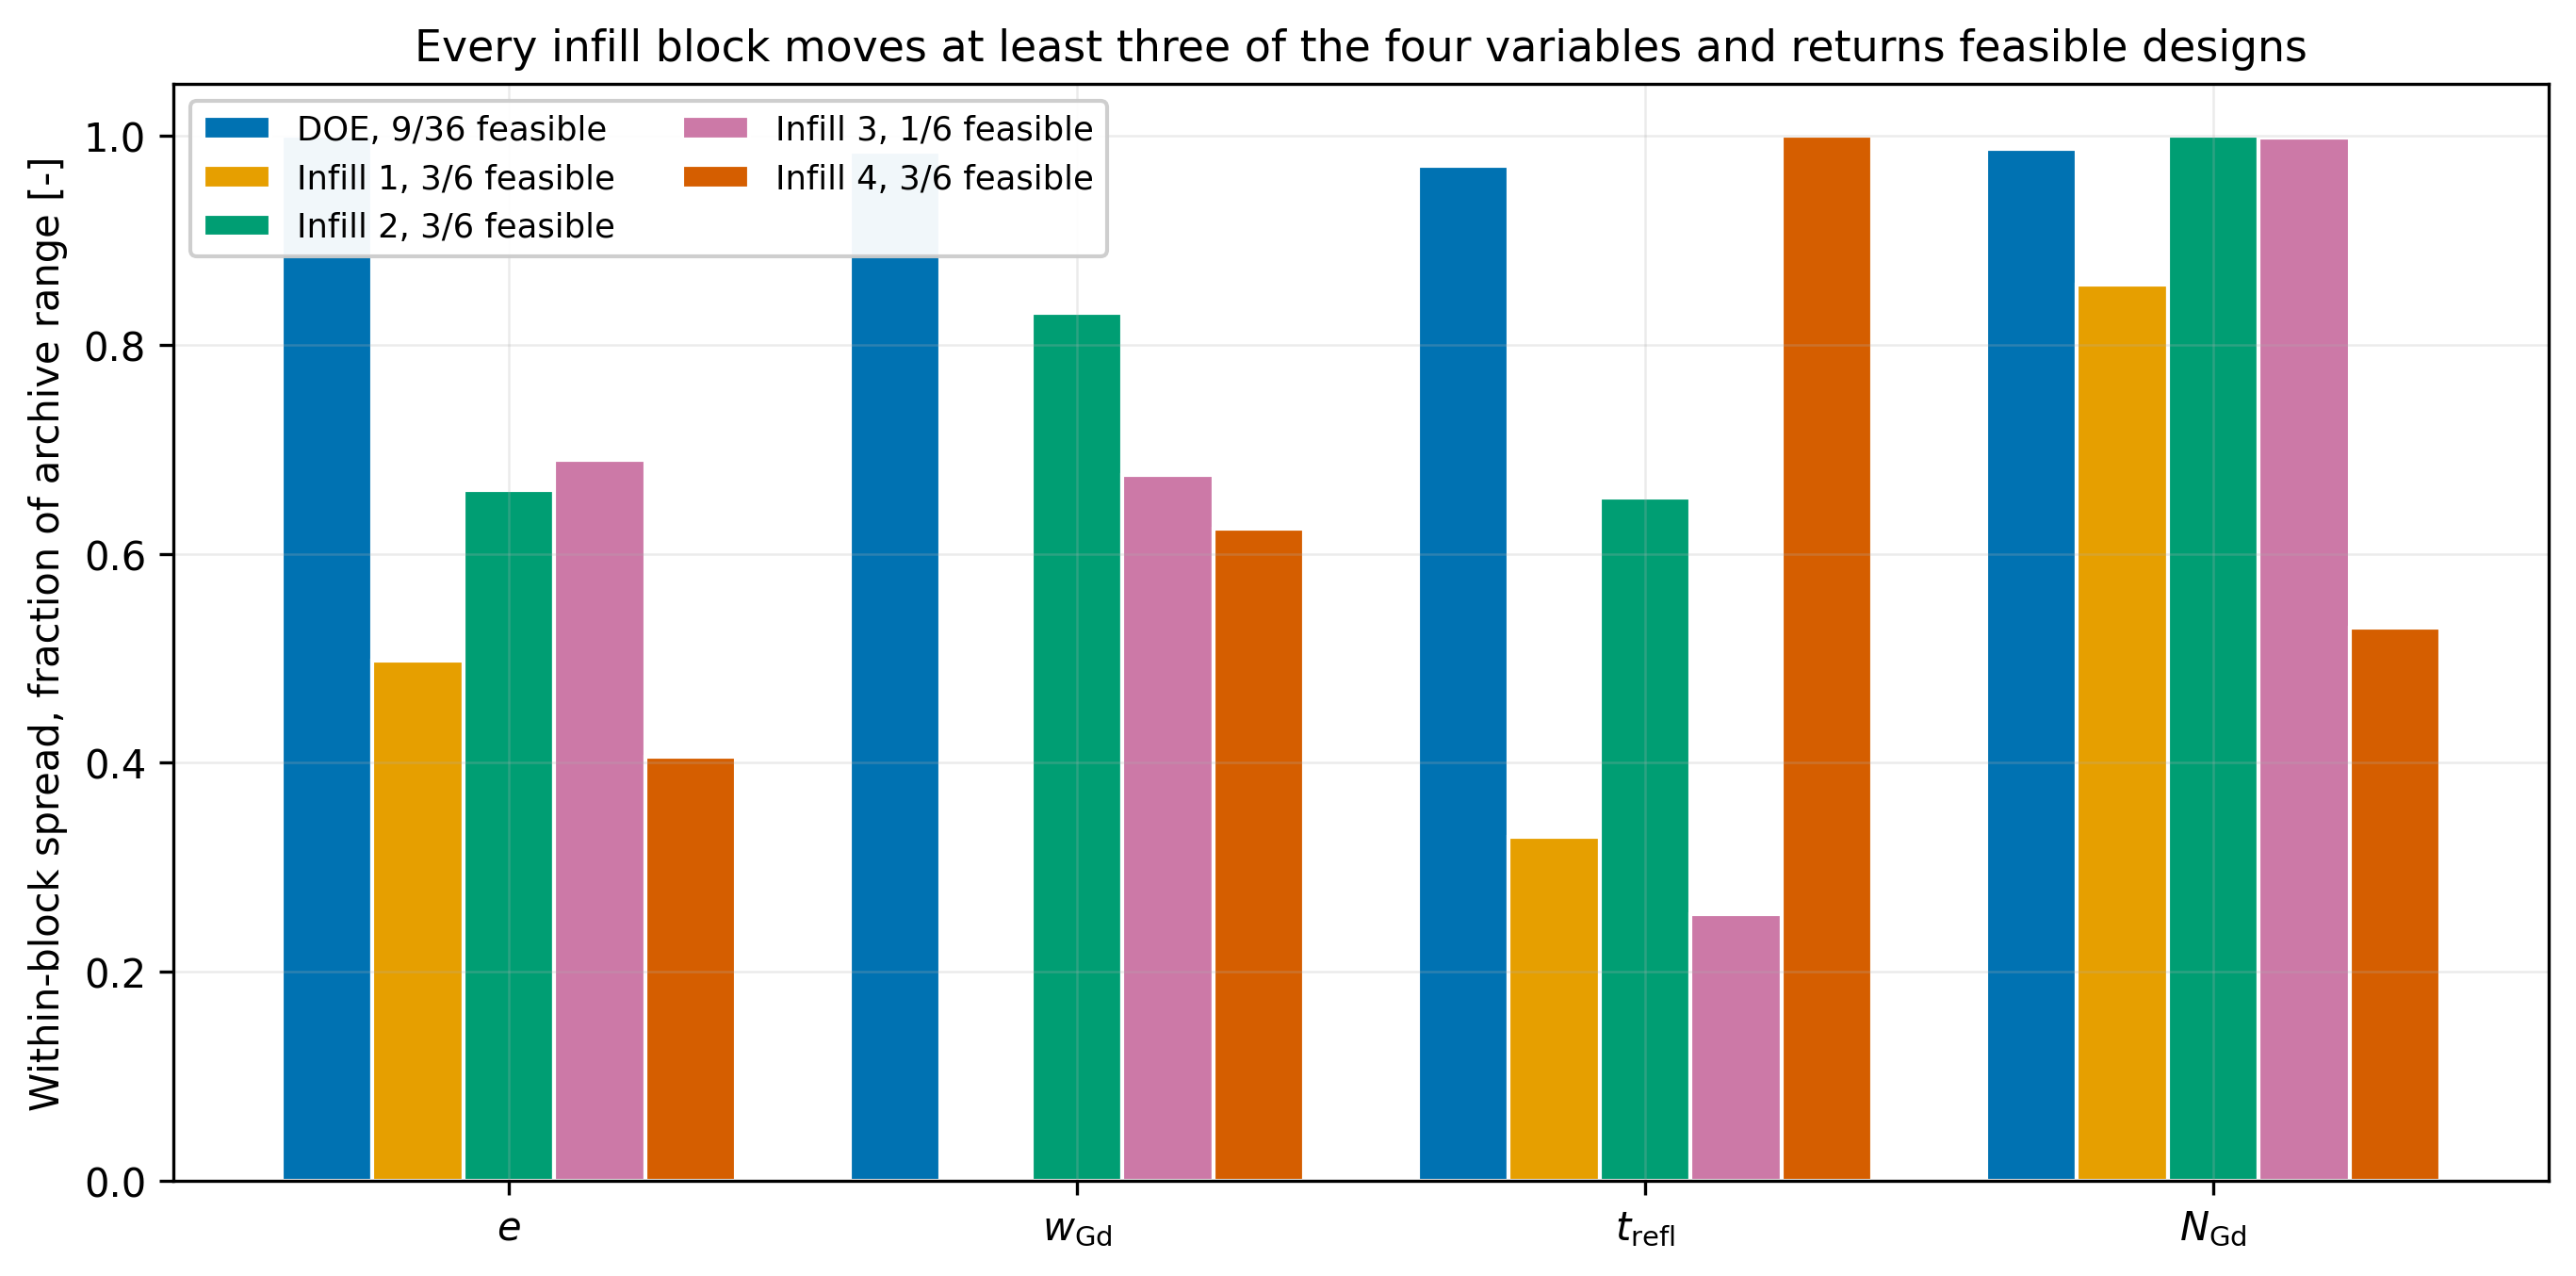
\includegraphics[width=\linewidth]{images/c8_infill_diversity}
  \caption{Within-block spread of each design variable in Campaign 8.}
  \label{fig:c8-diversity}
\end{figure}

\begin{figure}[htbp]
  \centering
  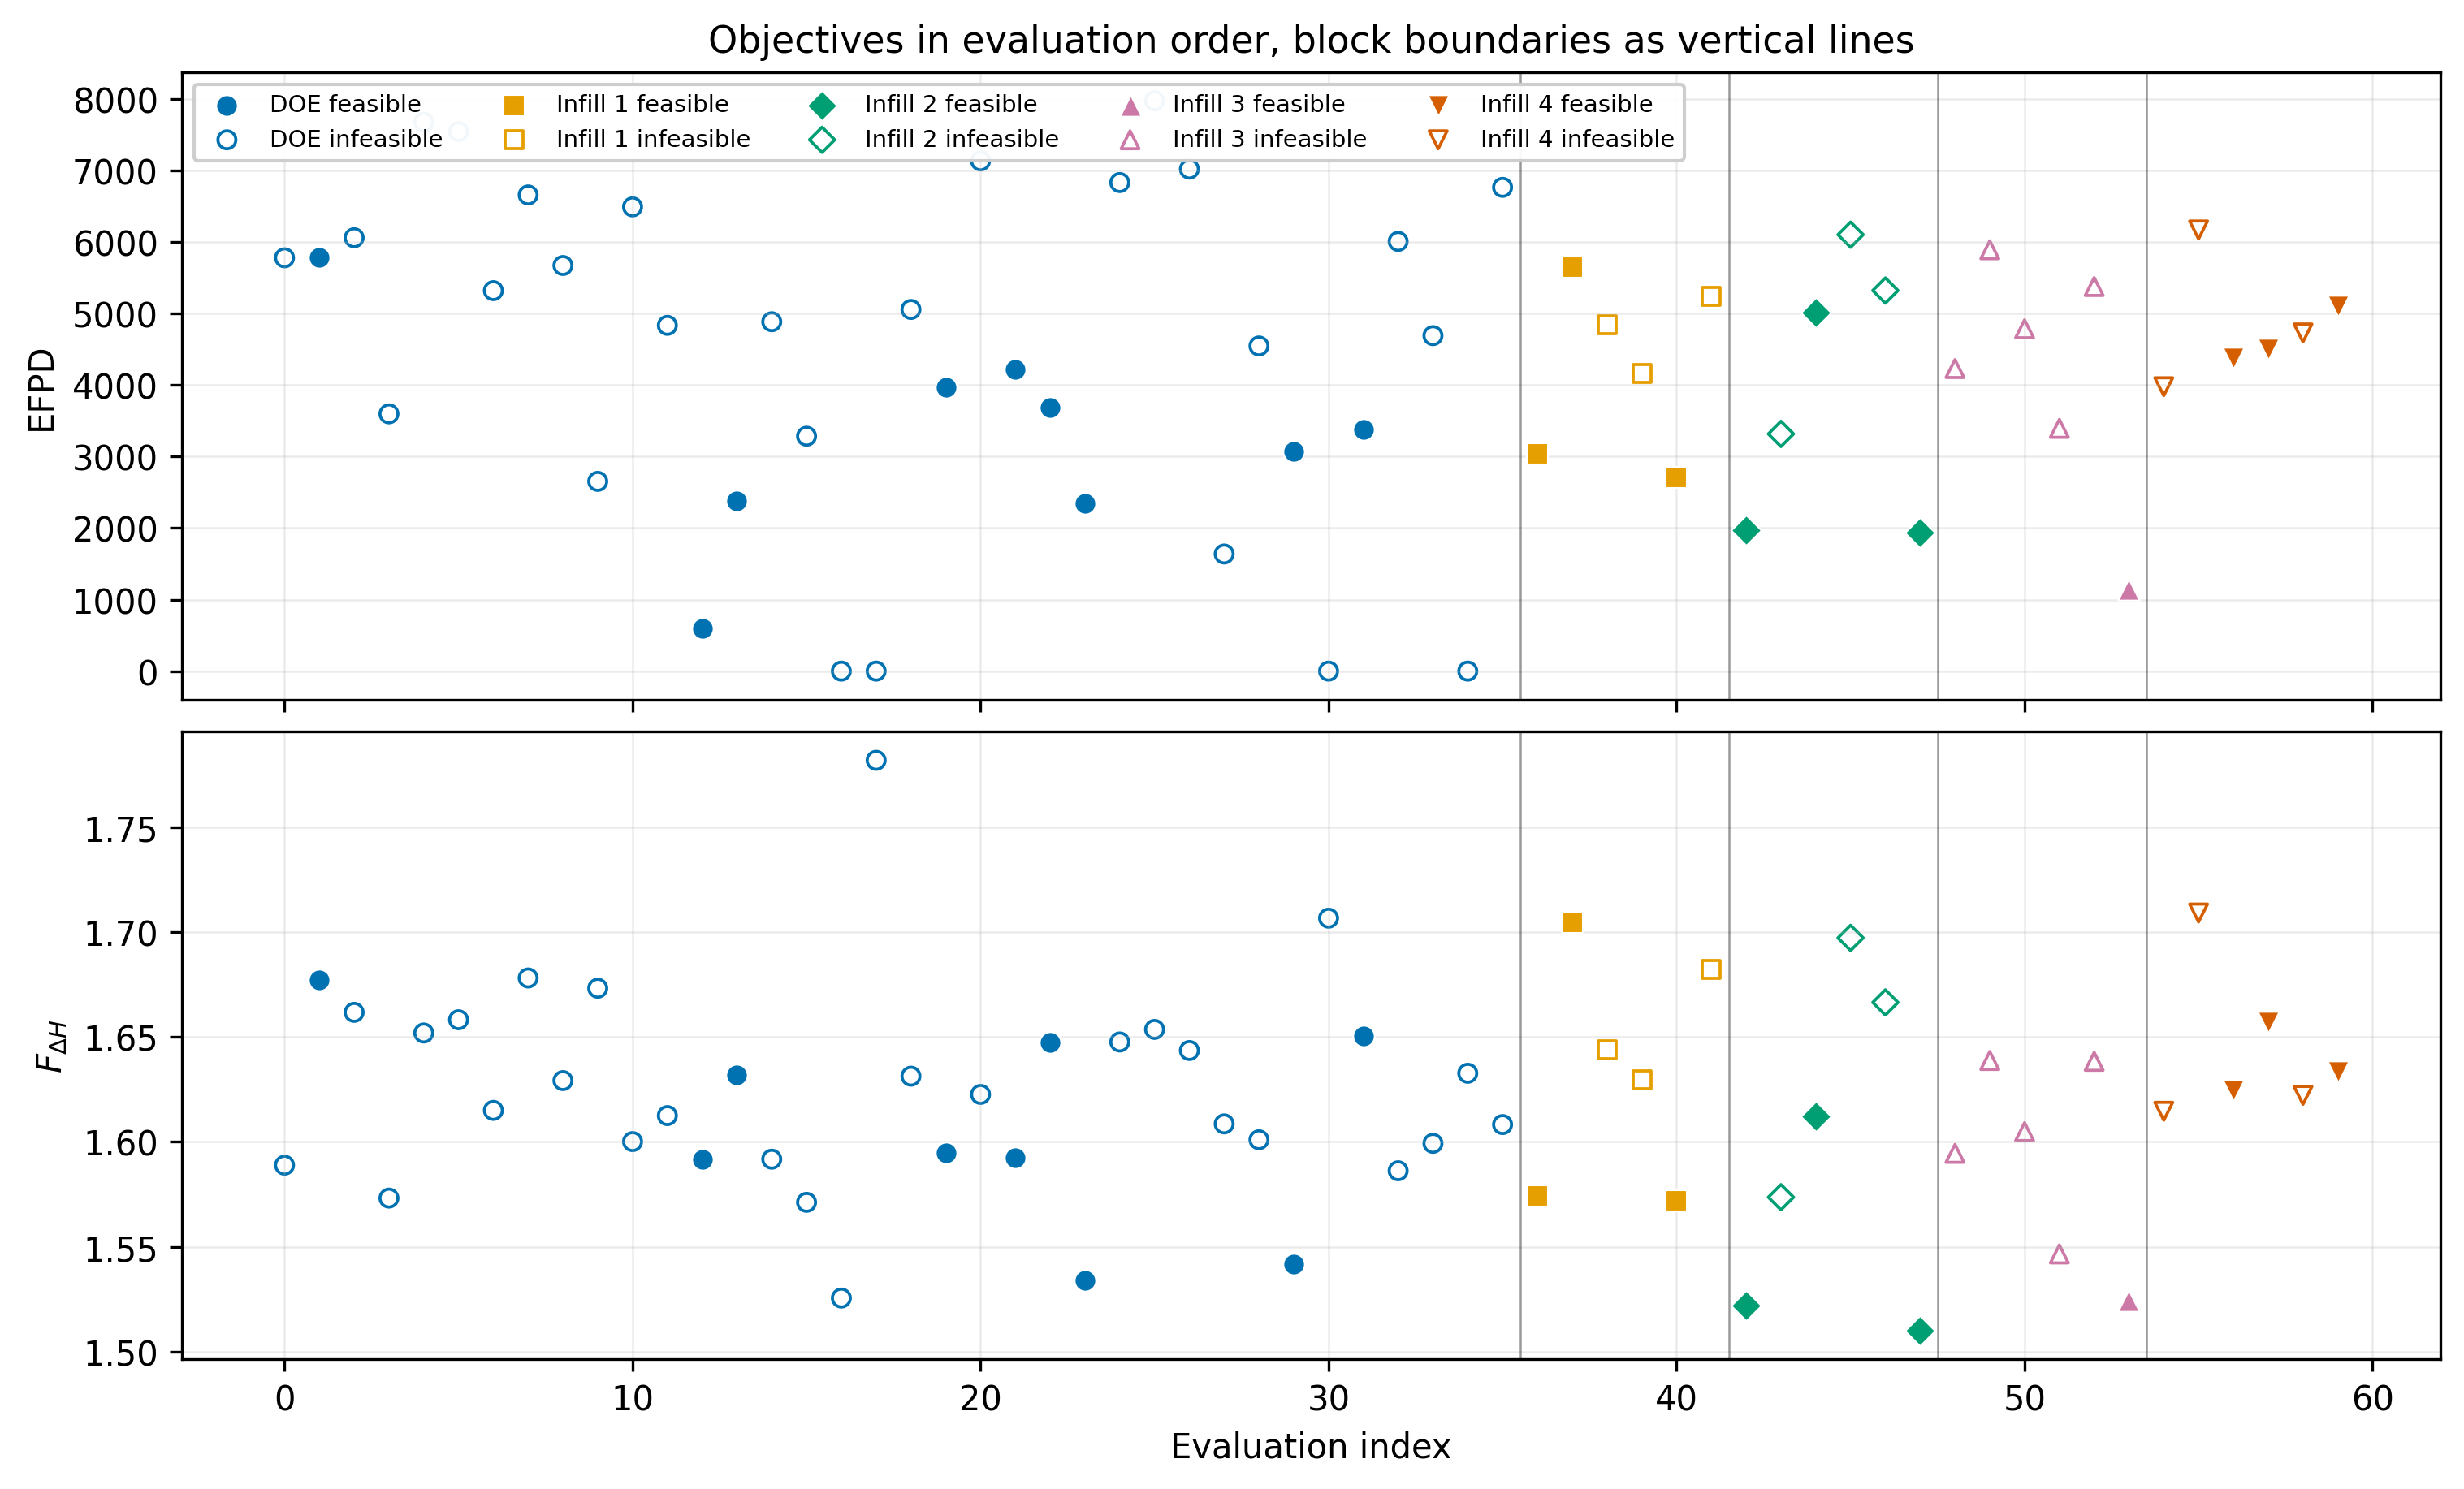
\includegraphics[width=\linewidth]{images/c8_trajectory}
  \caption{Campaign 8 objectives in evaluation order.}
  \label{fig:c8-trajectory}
\end{figure}

The convergence record is honest rather than complete. The hypervolume
gained \SI{2.87}{\%} in block 2 and then \SI{0.00}{\%} and
\SI{0.18}{\%} in blocks 3 and 4. Under the rule of
Section~\ref{sec:res-c6-blocks}, three consecutive gains below one per
cent with no censored design on the front, the campaign is one block
short of a formal stop. Unlike Campaign 7, the flat blocks here are not
acquisition failures: their designs are diverse and land on the
constraint boundary where the surrogate expects the front to be
(Figure~\ref{fig:c8-plane}). The front is therefore reported as
converged at the resolution the frozen reference can see, with the
stated caveat. In Figure~\ref{fig:c8-plane} the four-bank state on the
left is the constraint and the two-bank state on the right is recorded
only. The two-bank reading is subcritical only below an unrodded
eigenvalue of about 1.07.

\subsection{Feasibility and the binding constraint}
\label{sec:res-c8-screens}

Of the 60 designs, 19 are feasible, \SI{31.7}{\%}, with 9 of 36 in the
design of experiments. Table~\ref{tab:c8-nesting} gives the census and
Figure~\ref{fig:c8-activity} the activity per block. The nesting of
Campaign 7 is reversed: the ceiling never rejects a design that the
control screen accepts. The control screen
rejects 35 designs and is the dominant constraint in every block. No
design fails the peaking bound, the enrichment cap or the vessel fit.

\begin{table}[htbp]
  \centering
  \caption{Constraint census of Campaign 8 and the joint activity of the two reactivity screens.}
  \label{tab:c8-nesting}
  \begin{tabular}{lc}
    \toprule
    Outcome & Designs \\
    \midrule
    Fail $g_\mathrm{ctrl}$                          & 35 \\
    Fail $g_{k\max}$ at 1.166                       & 23 \\
    Fail $g_{k\max}$ and pass $g_\mathrm{ctrl}$     &  0 \\
    Fail $g_\mathrm{ctrl}$ and pass $g_{k\max}$     & 12 \\
    Fail $g_{k\min}$                                &  6 \\
    Feasible on all six                             & 19 \\
    Feasible and controllable with two banks        &  4 \\
    \bottomrule
  \end{tabular}
\end{table}

\begin{figure}[htbp]
  \centering
  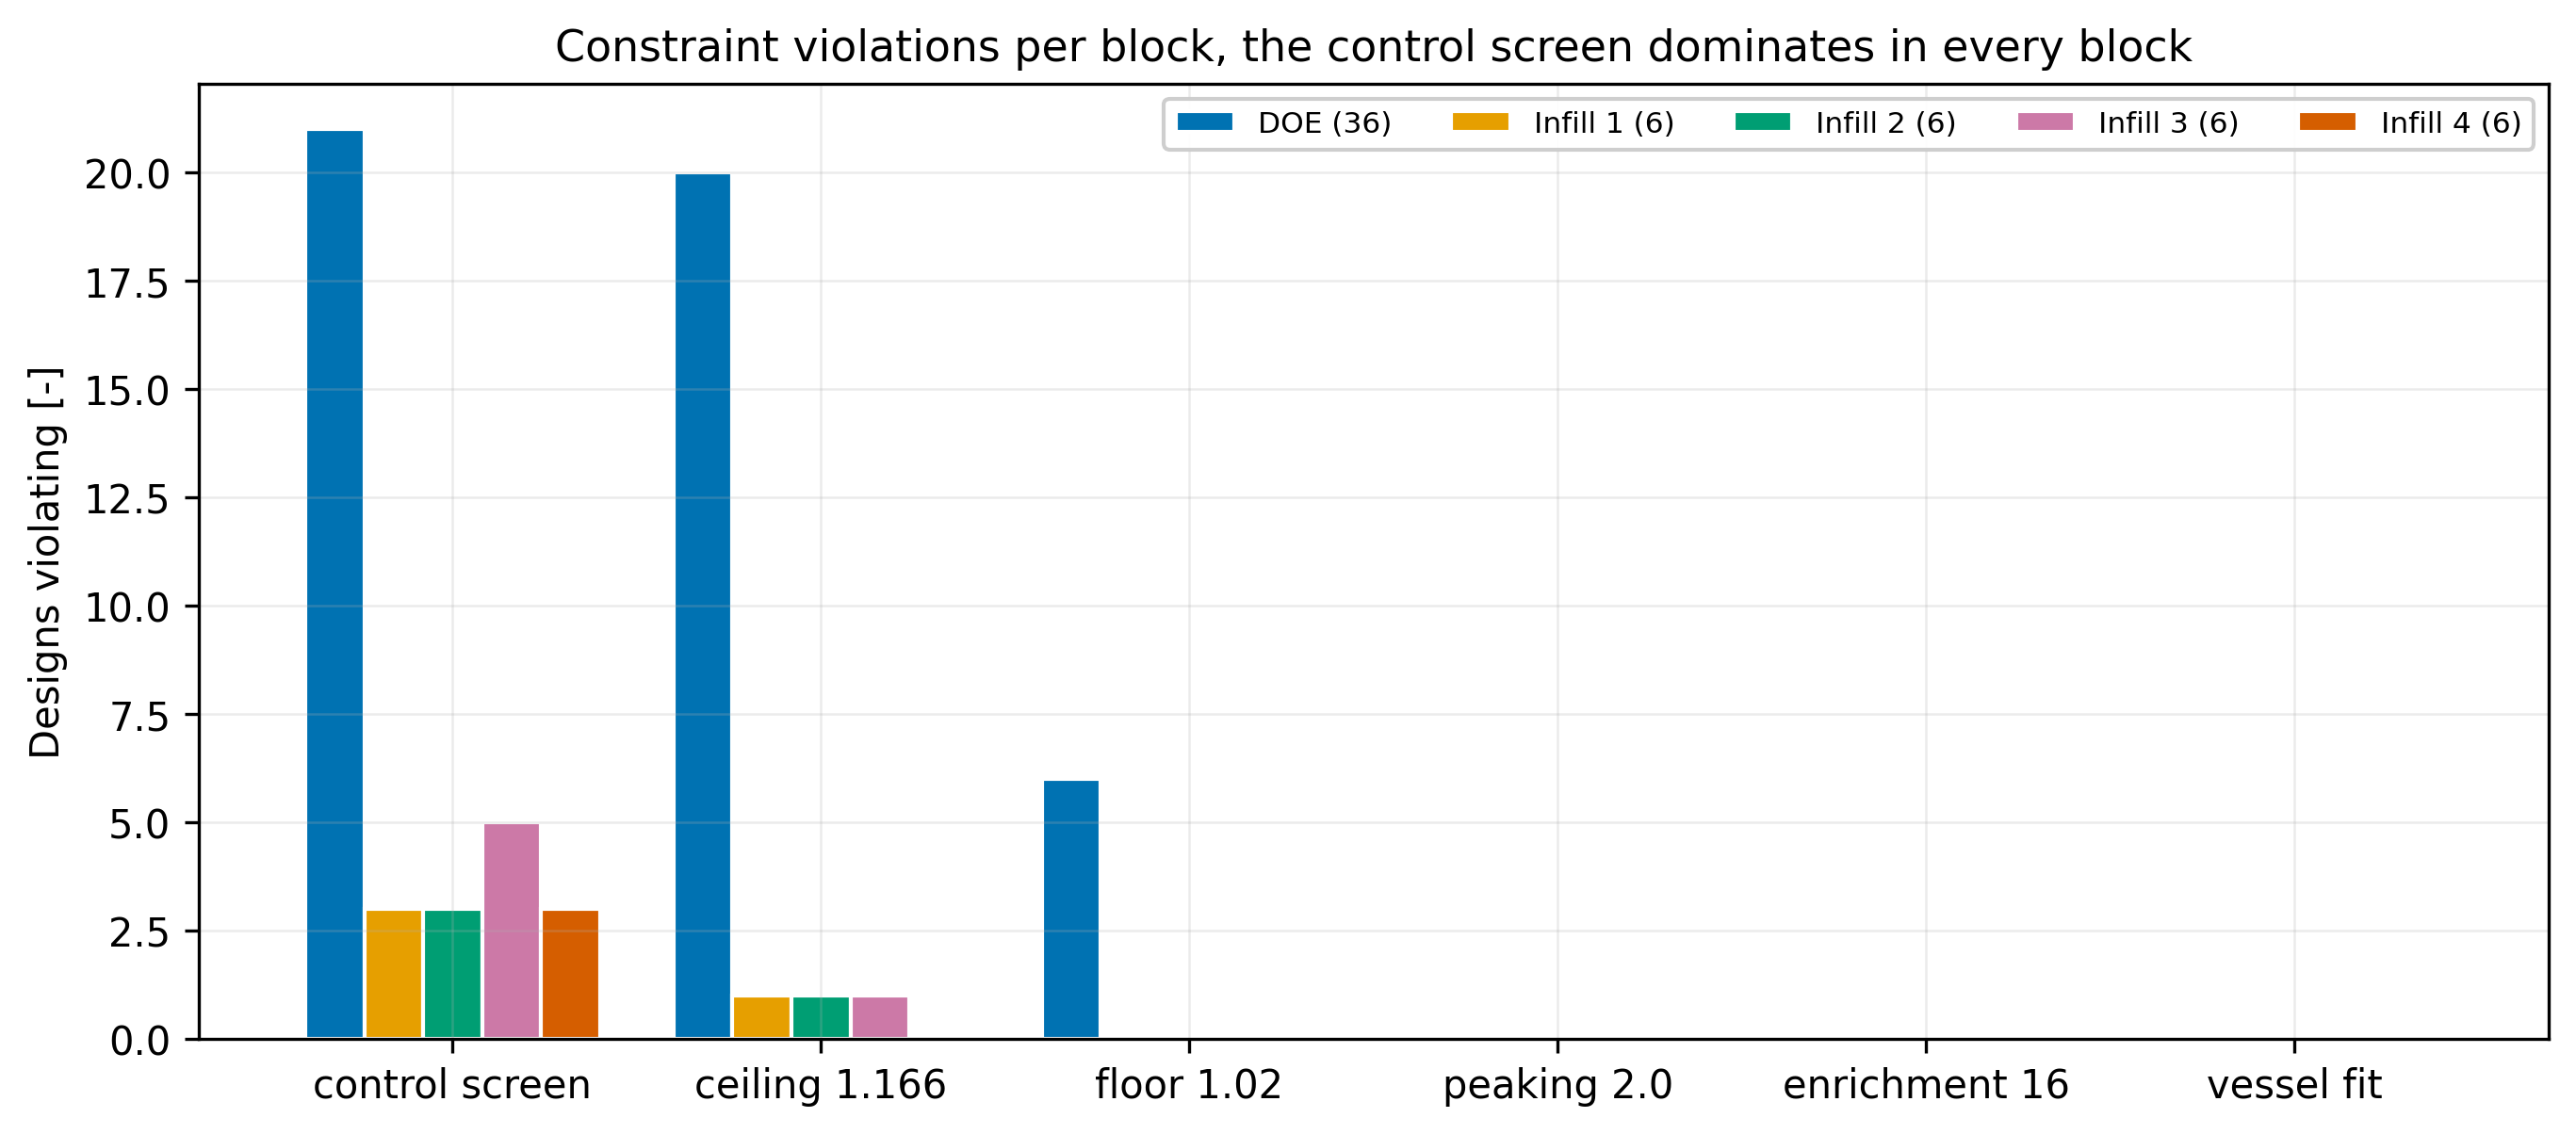
\includegraphics[width=\linewidth]{images/c8_constraint_activity}
  \caption{Campaign 8 constraint violations per block.}
  \label{fig:c8-activity}
\end{figure}

\begin{figure}[htbp]
  \centering
  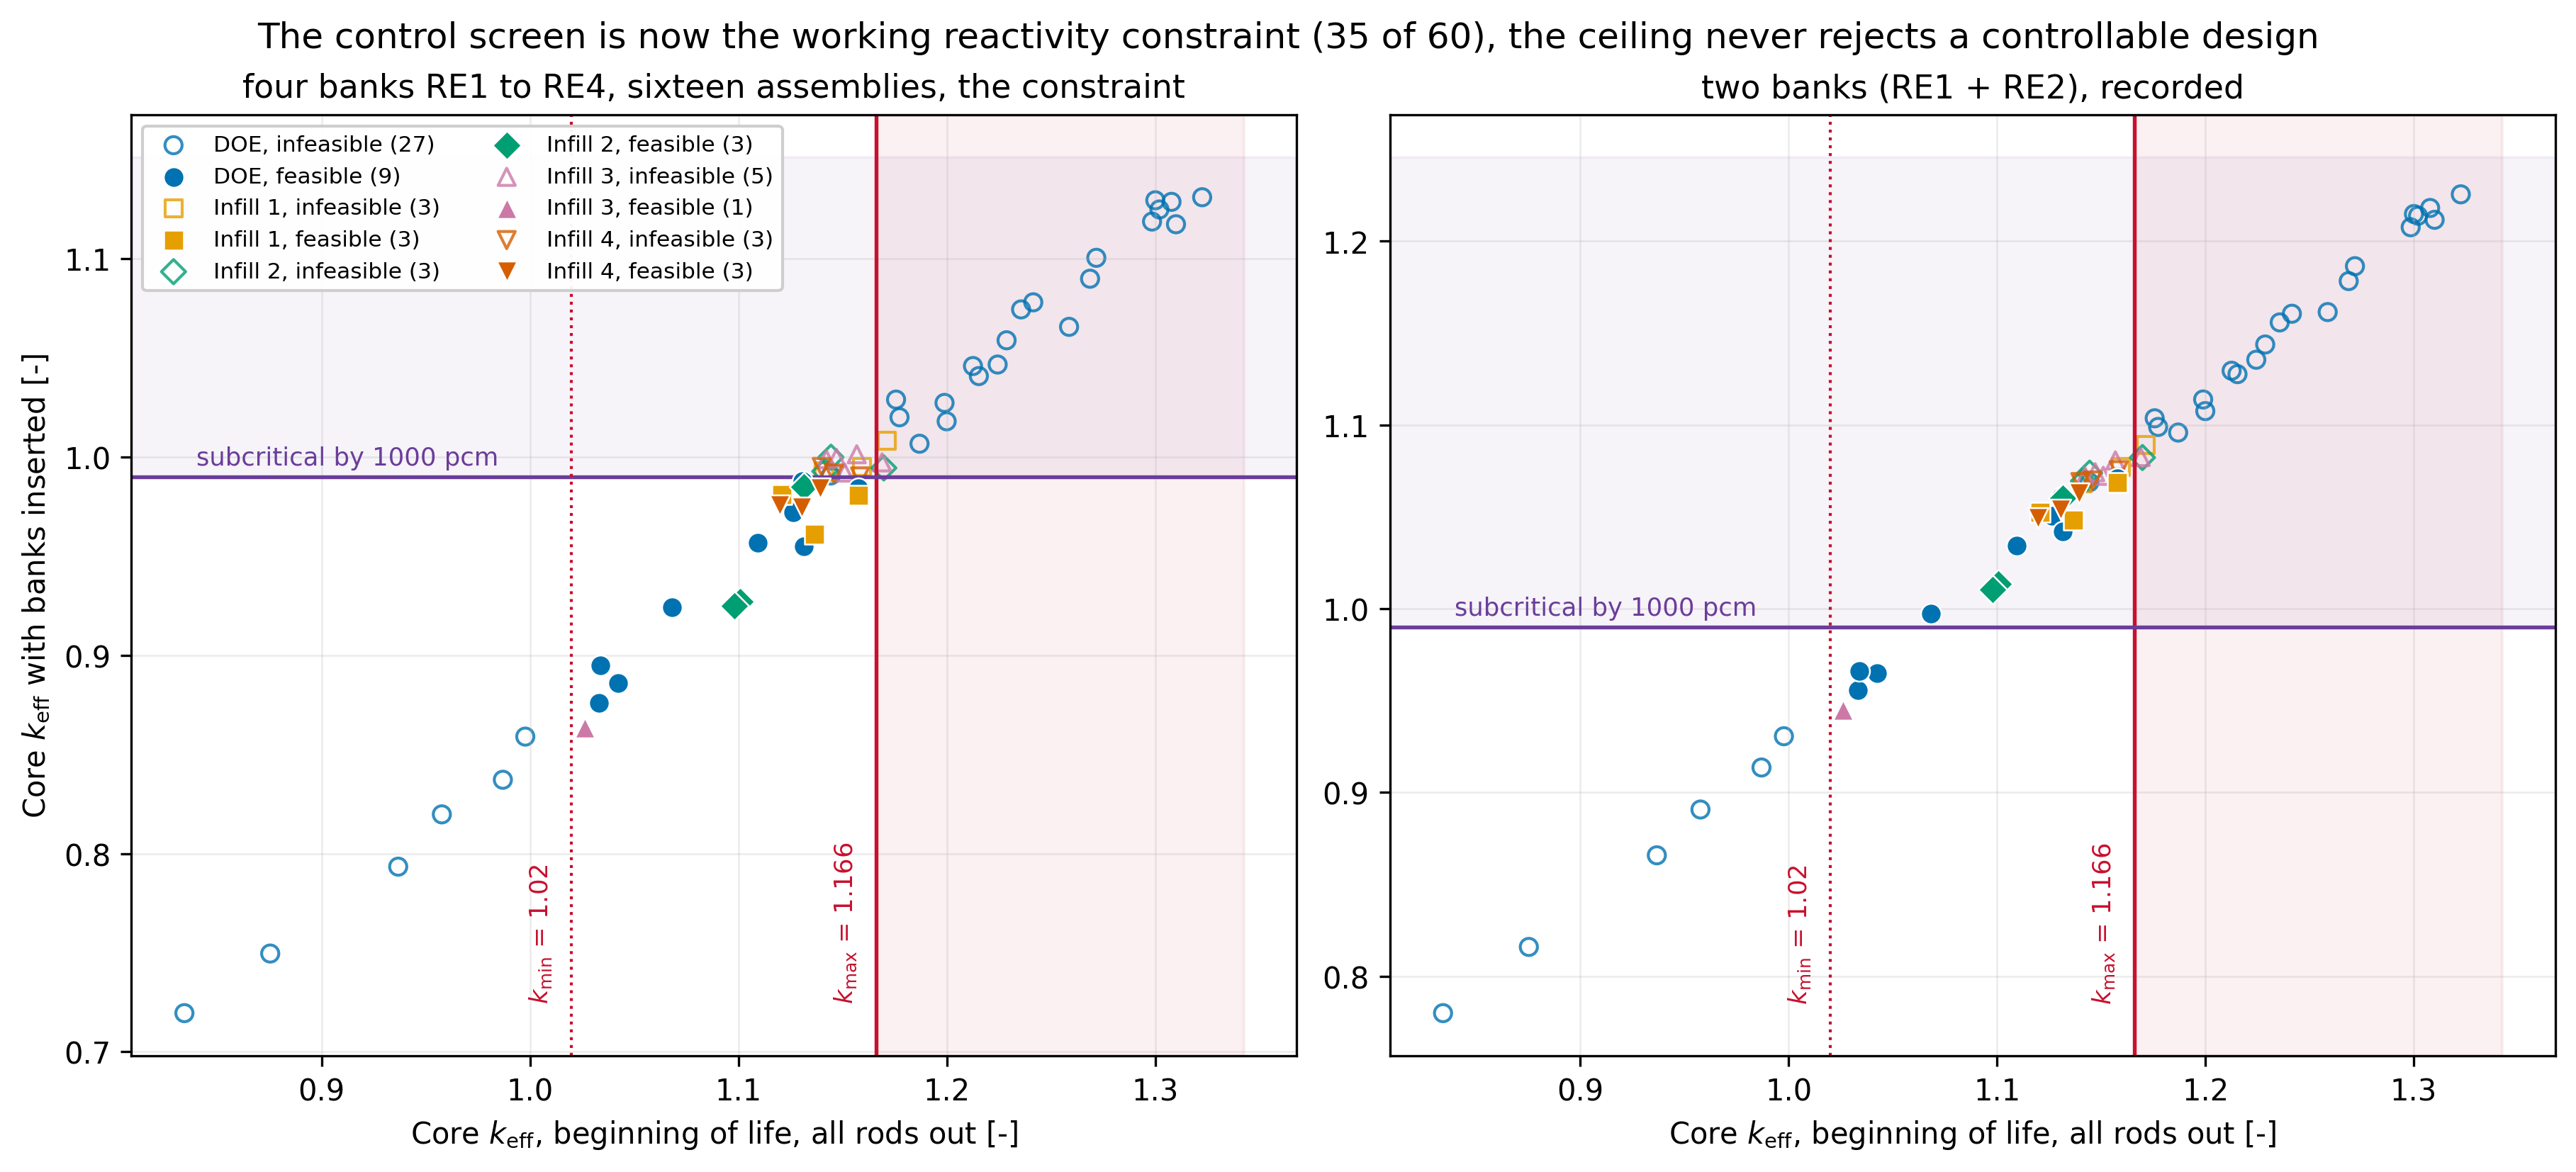
\includegraphics[width=\linewidth]{images/c8_ctrl_plane}
  \caption{Campaign 8 unrodded core eigenvalue against the eigenvalue with four banks inserted, left, and with two banks inserted, right.}
  \label{fig:c8-plane}
\end{figure}

This is the constraint architecture the campaign was built to produce.
Not one design fails the derived ceiling while passing the measured
screen, so the ceiling of 1.166 did no work, and twelve designs pass
the ceiling while failing the screen, so the screen did all of it. The
twelve are the long-cycle designs, from 3977 to 6169 EFPD, and they
fail by 17 to \SI{1135}{pcm} in the rodded eigenvalue. Two of them,
designs 54 and 11, fail by 17 and \SI{63}{pcm}, within the statistical
resolution of a single core solve, and are treated as marginal rather
than rejected in Section~\ref{sec:res-c8-limits}.

The bank worths of Equation~\eqref{eq:bank-worth} run from
\num{11466} to \SI{19313}{pcm} for the four banks and from
\num{5429} to \SI{9841}{pcm} for the first two, with the ratio between
\num{0.473} and \num{0.511} on all 60 designs and a mean of
\num{0.496}. Figure~\ref{fig:c8-worths} shows both against the two
absorber variables. At fixed pitch the gadolinium pin count is the
single driver, correlating at $-0.73$ with both worths, and the
concentration adds a weaker $-0.39$.

\begin{figure}[htbp]
  \centering
  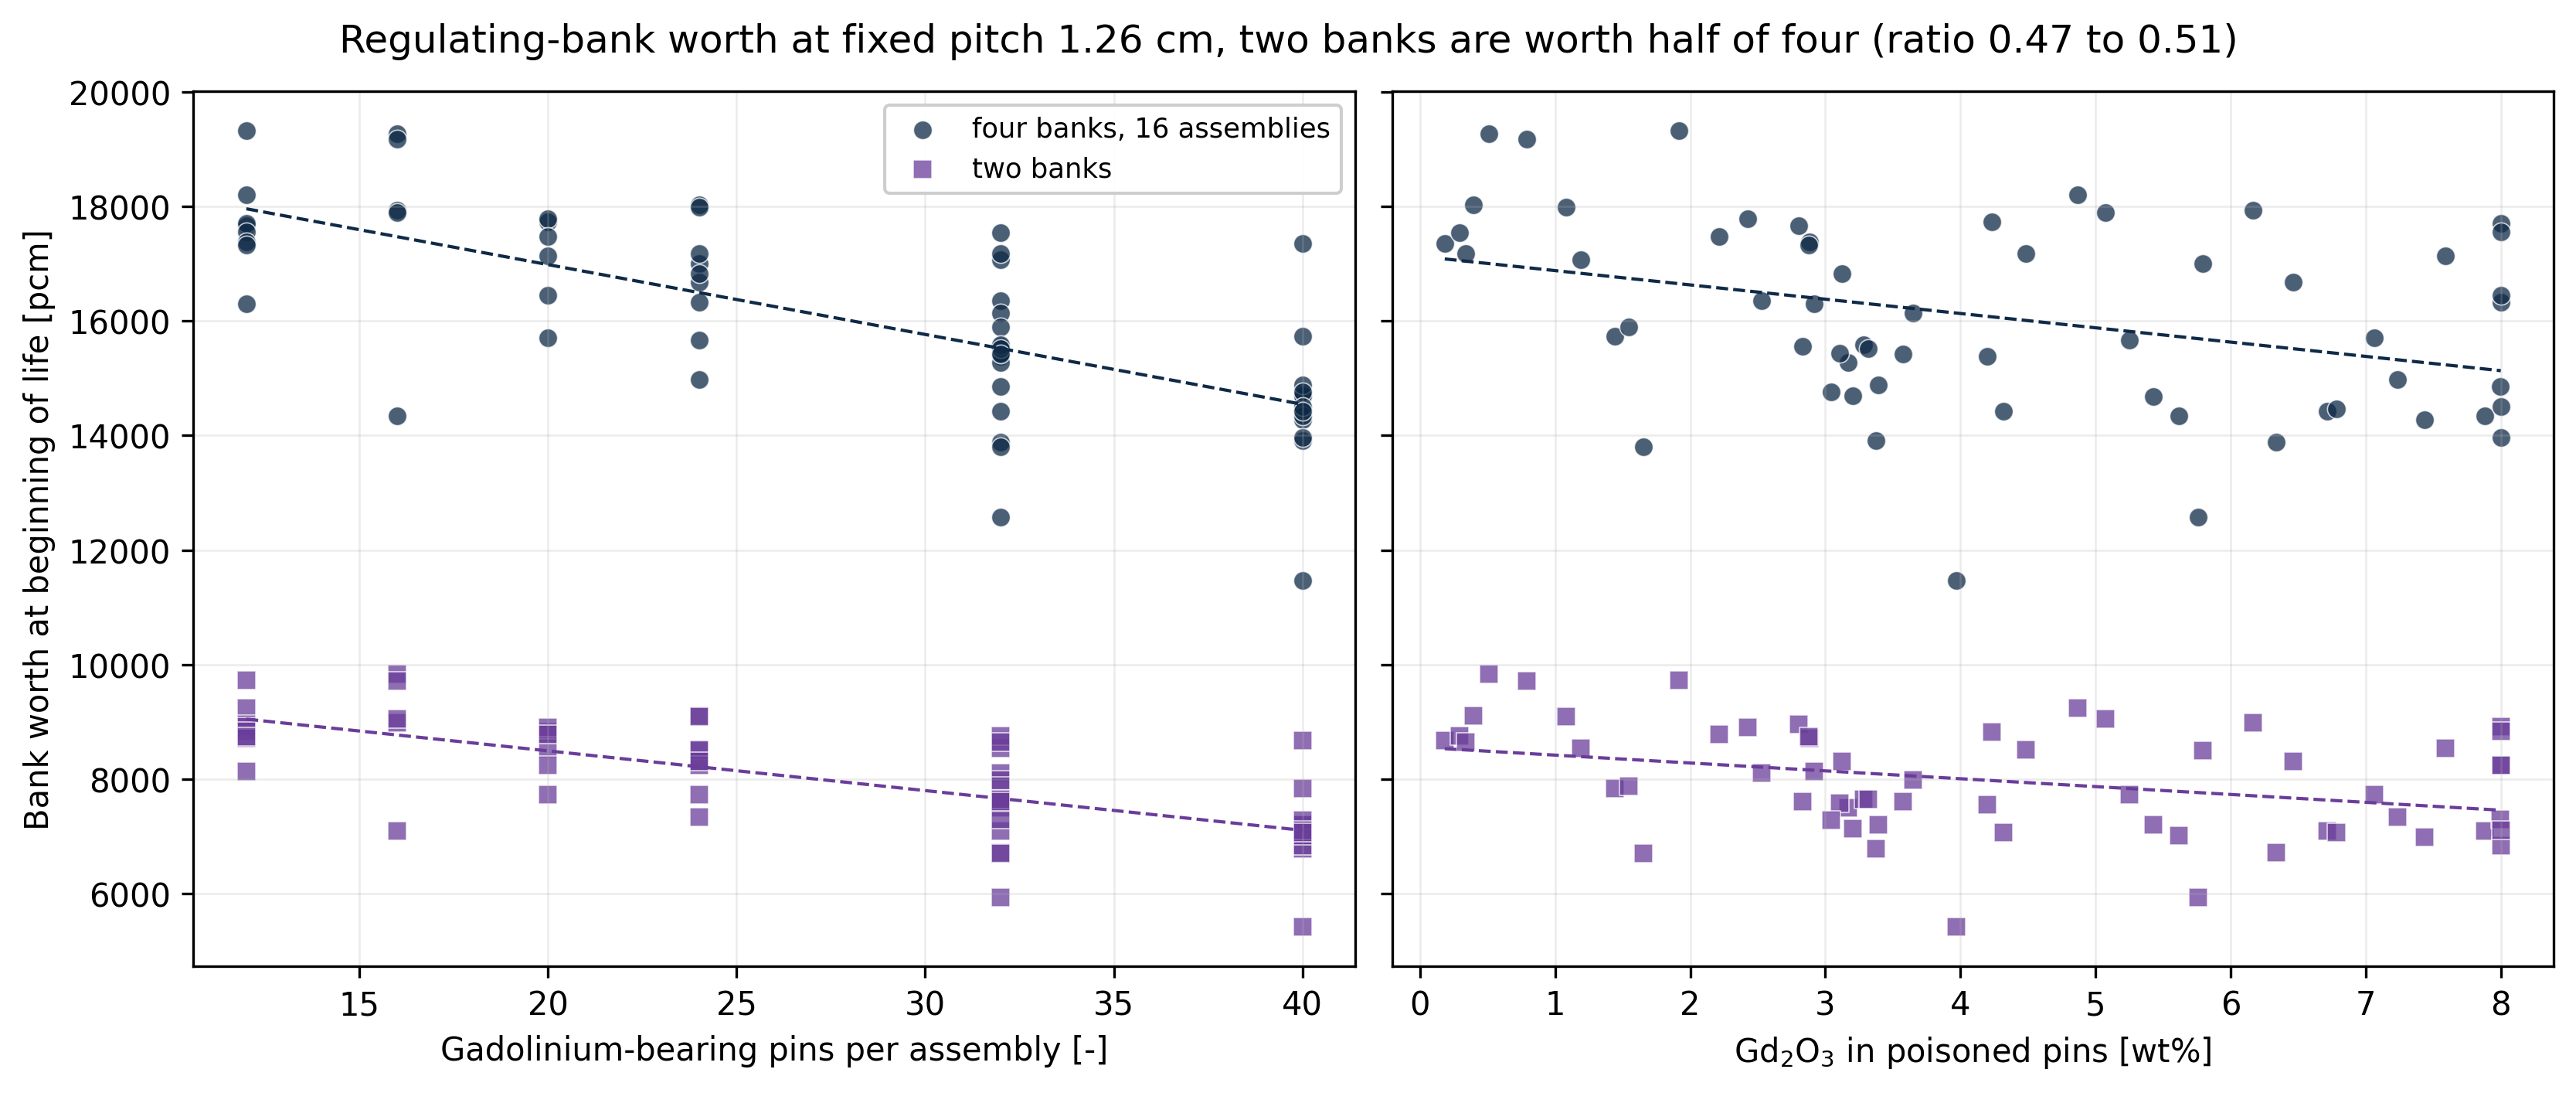
\includegraphics[width=\linewidth]{images/c8_worths}
  \caption{Regulating-bank worth at fixed pitch, four banks and two banks, against the gadolinium pin count and concentration.}
  \label{fig:c8-worths}
\end{figure}

The two-bank ceiling follows from the smallest two-bank worth as the
four-bank ceiling did in Section~\ref{sec:meth-ctrl}.

\begin{equation}
k_{\max}^{(2)} = (1 - \Delta\rho_\mathrm{op}) + \rho_\mathrm{bank}^{(2)}
\label{eq:two-bank-ceiling}
\end{equation}

\noindent where the symbols have the following meaning.

\begin{itemize}
  \item $k_{\max}^{(2)}$ is the highest unrodded eigenvalue that the
        first two banks alone can hold down at the margin,
        dimensionless.

  \item $\Delta\rho_\mathrm{op}$ is the operating margin, \num{0.01}.

  \item $\rho_\mathrm{bank}^{(2)}$ is the two-bank worth in units of
        $k$, \num{0.0543} to \num{0.0984} across the archive, median
        \num{0.0793}.
\end{itemize}

The median gives 1.069 and the minimum 1.044. The two-bank window
above the floor of 1.02 is therefore about \SI{5000}{pcm} wide, against
\SI{13000}{pcm} for four banks, and it holds four of the nineteen
feasible designs.

\subsection{The front}
\label{sec:res-c8-front}

The feasible non-dominated set holds eight designs, from 1941 to 5782
EFPD and from $F_{\Delta H}$ 1.510 to 1.677. Table~\ref{tab:c8-front}
lists them and Figure~\ref{fig:c8-pareto} places every design in the
objective plane with its block. In the table the ring enrichments are
the as-built centre, middle and periphery values, the excess is the
beginning-of-life reactivity at \SI{1000}{ppm} that the rods must hold,
and the peaking factor is given with all rods out ($F$), with two banks
in ($F_2$) and with four banks in ($F_{16}$). In the figure filled
markers are feasible, purple rings mark the four feasible designs
controllable with the first two banks alone, and the vertical dotted
lines are five calendar years at capacity factors of 0.5 and 0.8. Four
front designs come from the
design of experiments, three from infill block 2 and one from block 4.
The discharge screen of \SI{75}{MWd/kgHM} is inactive on the front,
whose highest end-of-cycle burnup is \SI{57.7}{MWd/kgHM}, and no
design is censored.

\begin{table}[htbp]
  \centering
  \small
  \caption[The Campaign 8 front]{The Campaign 8 front.}
  \label{tab:c8-front}
  \setlength{\tabcolsep}{3.4pt}
  \begin{tabular}{ccccccccccc}
    \toprule
    Design & EFPD & rings & $w_\mathrm{Gd}$ & $n_\mathrm{Gd}$ &
      $t_\mathrm{refl}$ & $k^\mathrm{core}$ & excess & $F$ & $F_{2}$ &
      $F_{16}$ \\
    {[--]} & [d] & [wt\%] & [wt\%] & [rods] & [cm] & [--] & [pcm] &
      [--] & [--] & [--] \\
    \midrule
    47 & 1941 & 3.16, 3.93, 5.05  & 2.88 & 12 & 4.29 & 1.098 &  8930 & 1.510 & 1.991 & 2.314 \\
    42 & 1968 & 3.20, 3.97, 5.11  & 2.88 & 12 & 3.76 & 1.101 &  9154 & 1.522 & 1.997 & 2.264 \\
    23 & 2346 & 3.56, 4.42, 5.68  & 2.80 & 12 & 4.81 & 1.132 & 11626 & 1.534 & 1.968 & 2.356 \\
    29 & 3070 & 4.25, 5.27, 6.79  & 0.18 & 40 & 4.69 & 1.158 & 13627 & 1.542 & 1.935 & 2.218 \\
    21 & 4221 & 5.63, 6.98, 8.99  & 3.11 & 32 & 4.92 & 1.126 & 11220 & 1.592 & 1.934 & 2.194 \\
    44 & 5019 & 6.65, 8.25, 10.61 & 3.20 & 40 & 5.33 & 1.132 & 11631 & 1.612 & 1.996 & 2.177 \\
    59 & 5104 & 6.73, 8.35, 10.75 & 4.32 & 40 & 5.66 & 1.120 & 10701 & 1.634 & 1.998 & 2.214 \\
     1 & 5782 & 7.94, 9.85, 12.68 & 7.43 & 40 & 3.94 & 1.131 & 11554 & 1.677 & 2.007 & 2.210 \\
    \bottomrule
  \end{tabular}
\end{table}

\begin{figure}[htbp]
  \centering
  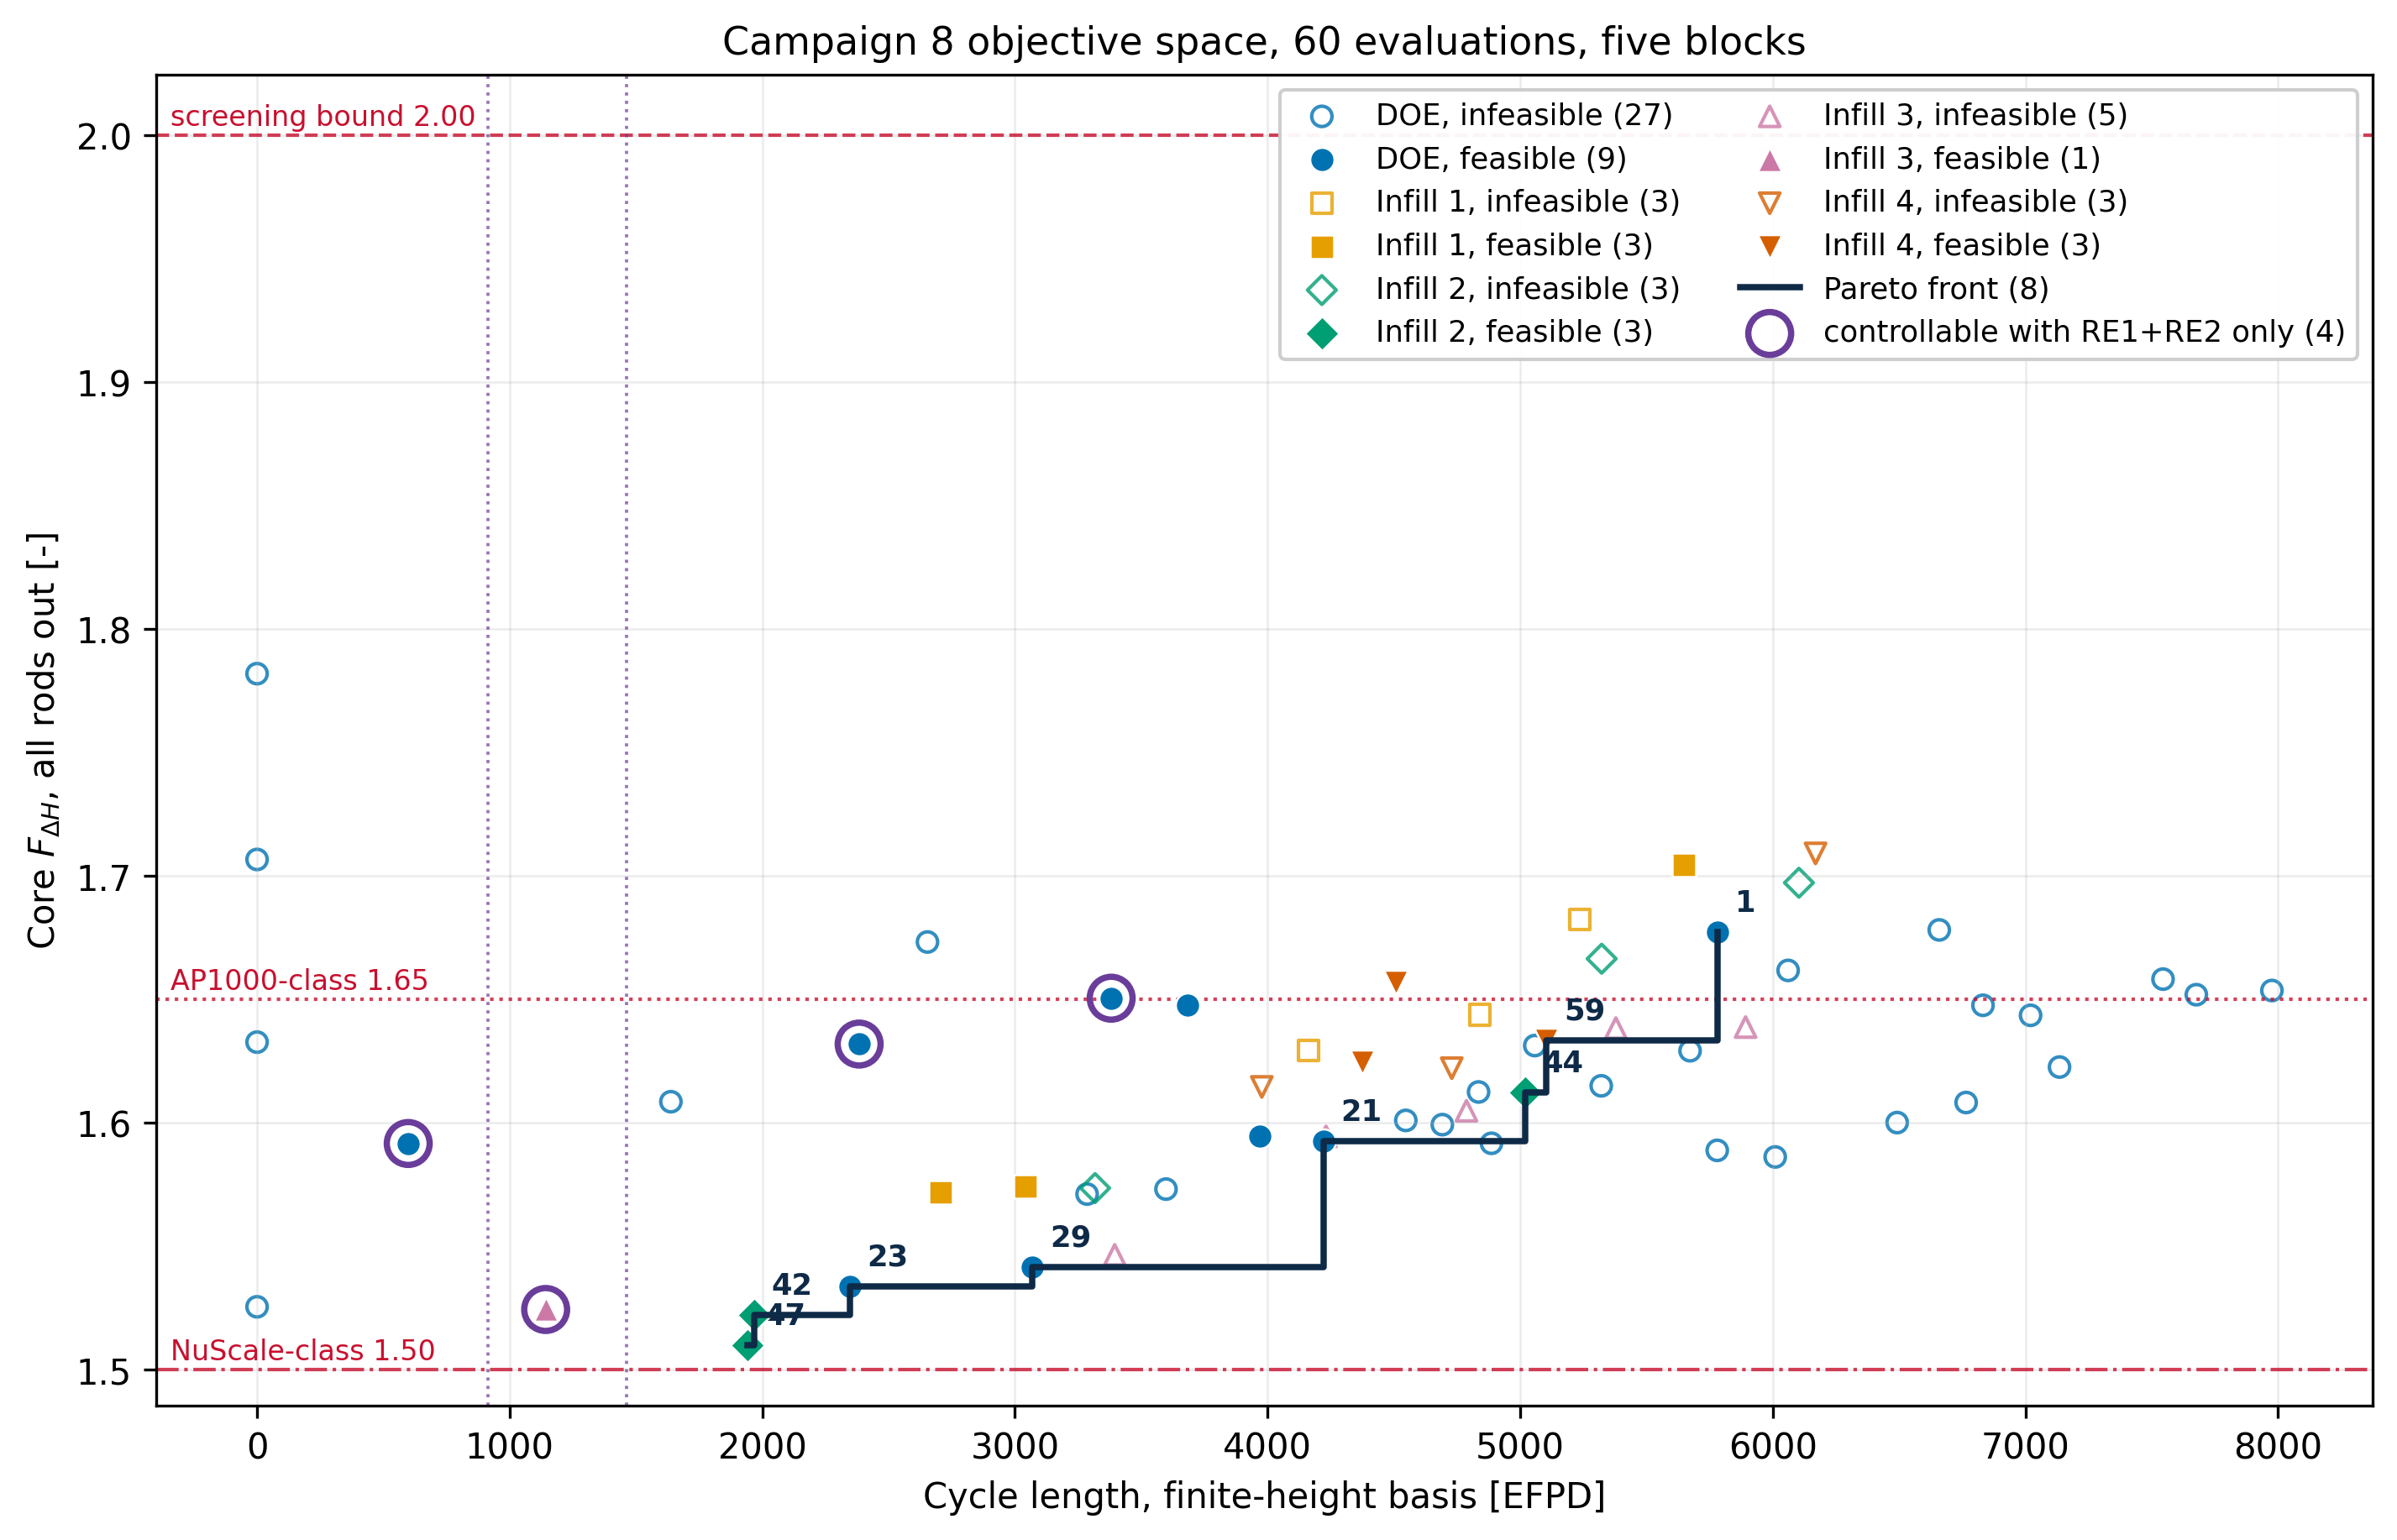
\includegraphics[width=\linewidth]{images/c8_pareto}
  \caption{Campaign 8 objective space with the five blocks distinguished.}
  \label{fig:c8-pareto}
\end{figure}

Three features of the front carry into the candidate discussion.

\begin{enumerate}
  \item The peaking floor did not rise. The pre-registered expectation
        was a floor near 1.60, on the argument that the low-peaking end
        of the Campaign 7 front lived at thick reflectors that the fixed
        pitch cannot accommodate. The Campaign 8 floor is 1.510, at
        design 47, and it is reached by a different route: a low uniform
        enrichment with twelve poisoned pins and a short cycle. The
        reflector lever was removed and the enrichment lever took its
        place. Peaking correlates at $+0.82$ with enrichment over the
        feasible set (Figure~\ref{fig:c8-influence}).

  \item Every front design sits on the control boundary. The unrodded
        eigenvalues run from 1.098 to 1.158, and the rodded eigenvalues
        from 0.925 to 0.988, so the beginning-of-life excess that the
        four banks must hold lies between \num{8930} and
        \SI{13627}{pcm} with the soluble boron already in the coolant.
        Design 29, with \SI{0.18}{wt\%} gadolinia on forty pins, is
        effectively unpoisoned and carries the largest excess.

  \item The two-bank peaking of every front design is 1.93 to 2.01.
        With only RE1 and RE2 inserted the front sits on the screening
        bound, and with all four banks it exceeds it by 0.18 to 0.36
        (Figure~\ref{fig:c8-split}). The rodded peaking is a property of
        the map, not of the design: over all 60 designs the two-bank
        value spans only 1.82 to 2.35.
\end{enumerate}

\begin{figure}[htbp]
  \centering
  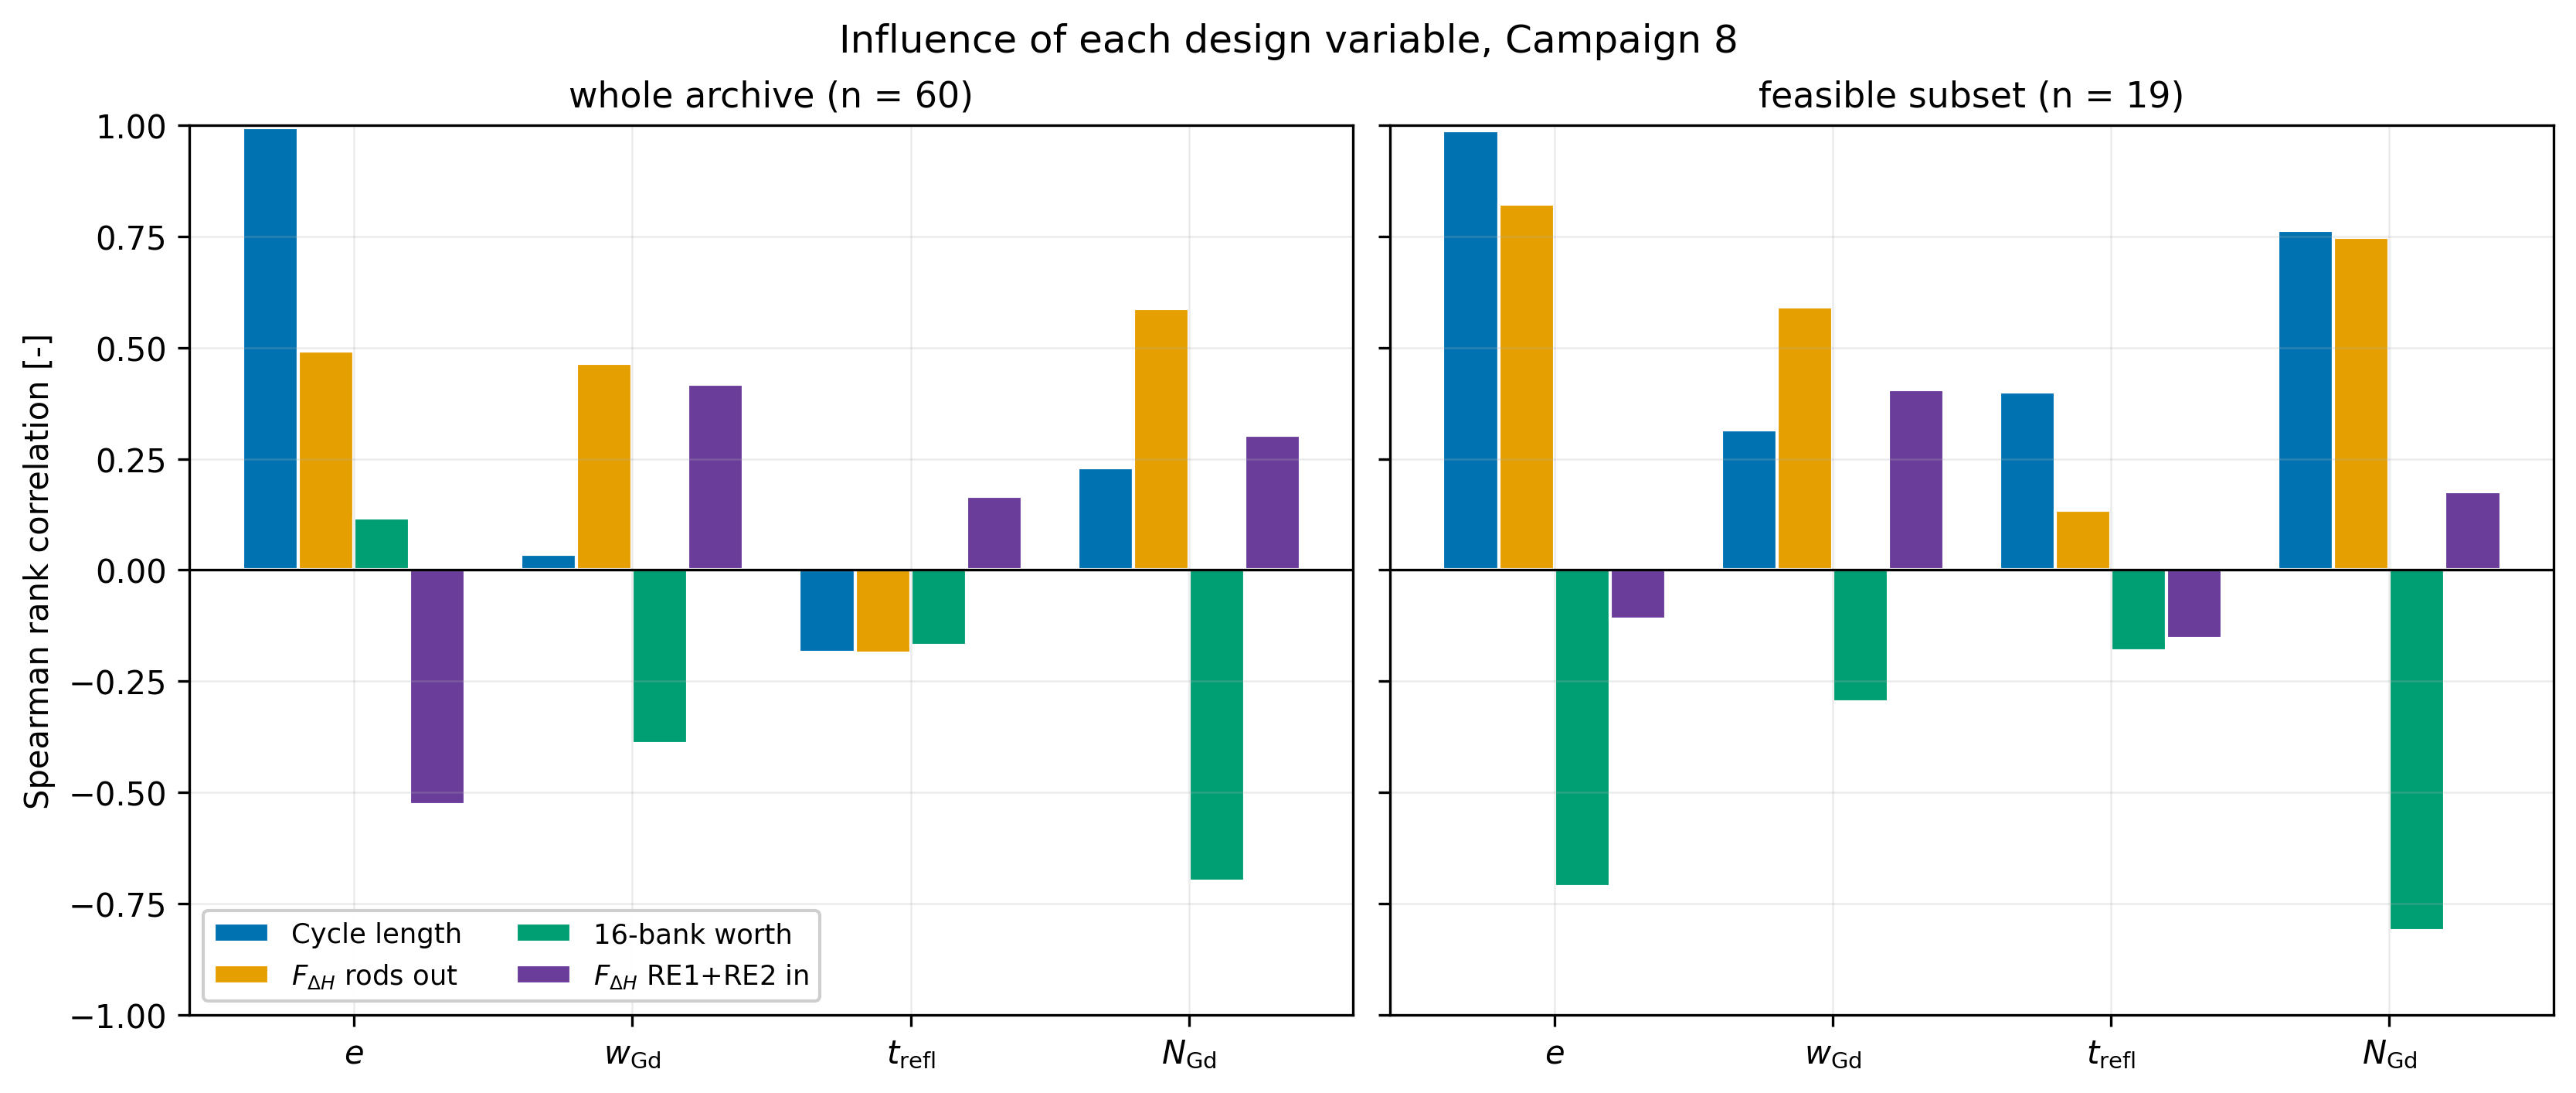
\includegraphics[width=\linewidth]{images/c8_vars_influence}
  \caption{Spearman rank correlation of each design variable with the
  objectives, the four-bank worth and the two-bank peaking, over the
  archive and over the feasible subset.}
  \label{fig:c8-influence}
\end{figure}

\begin{figure}[htbp]
  \centering
  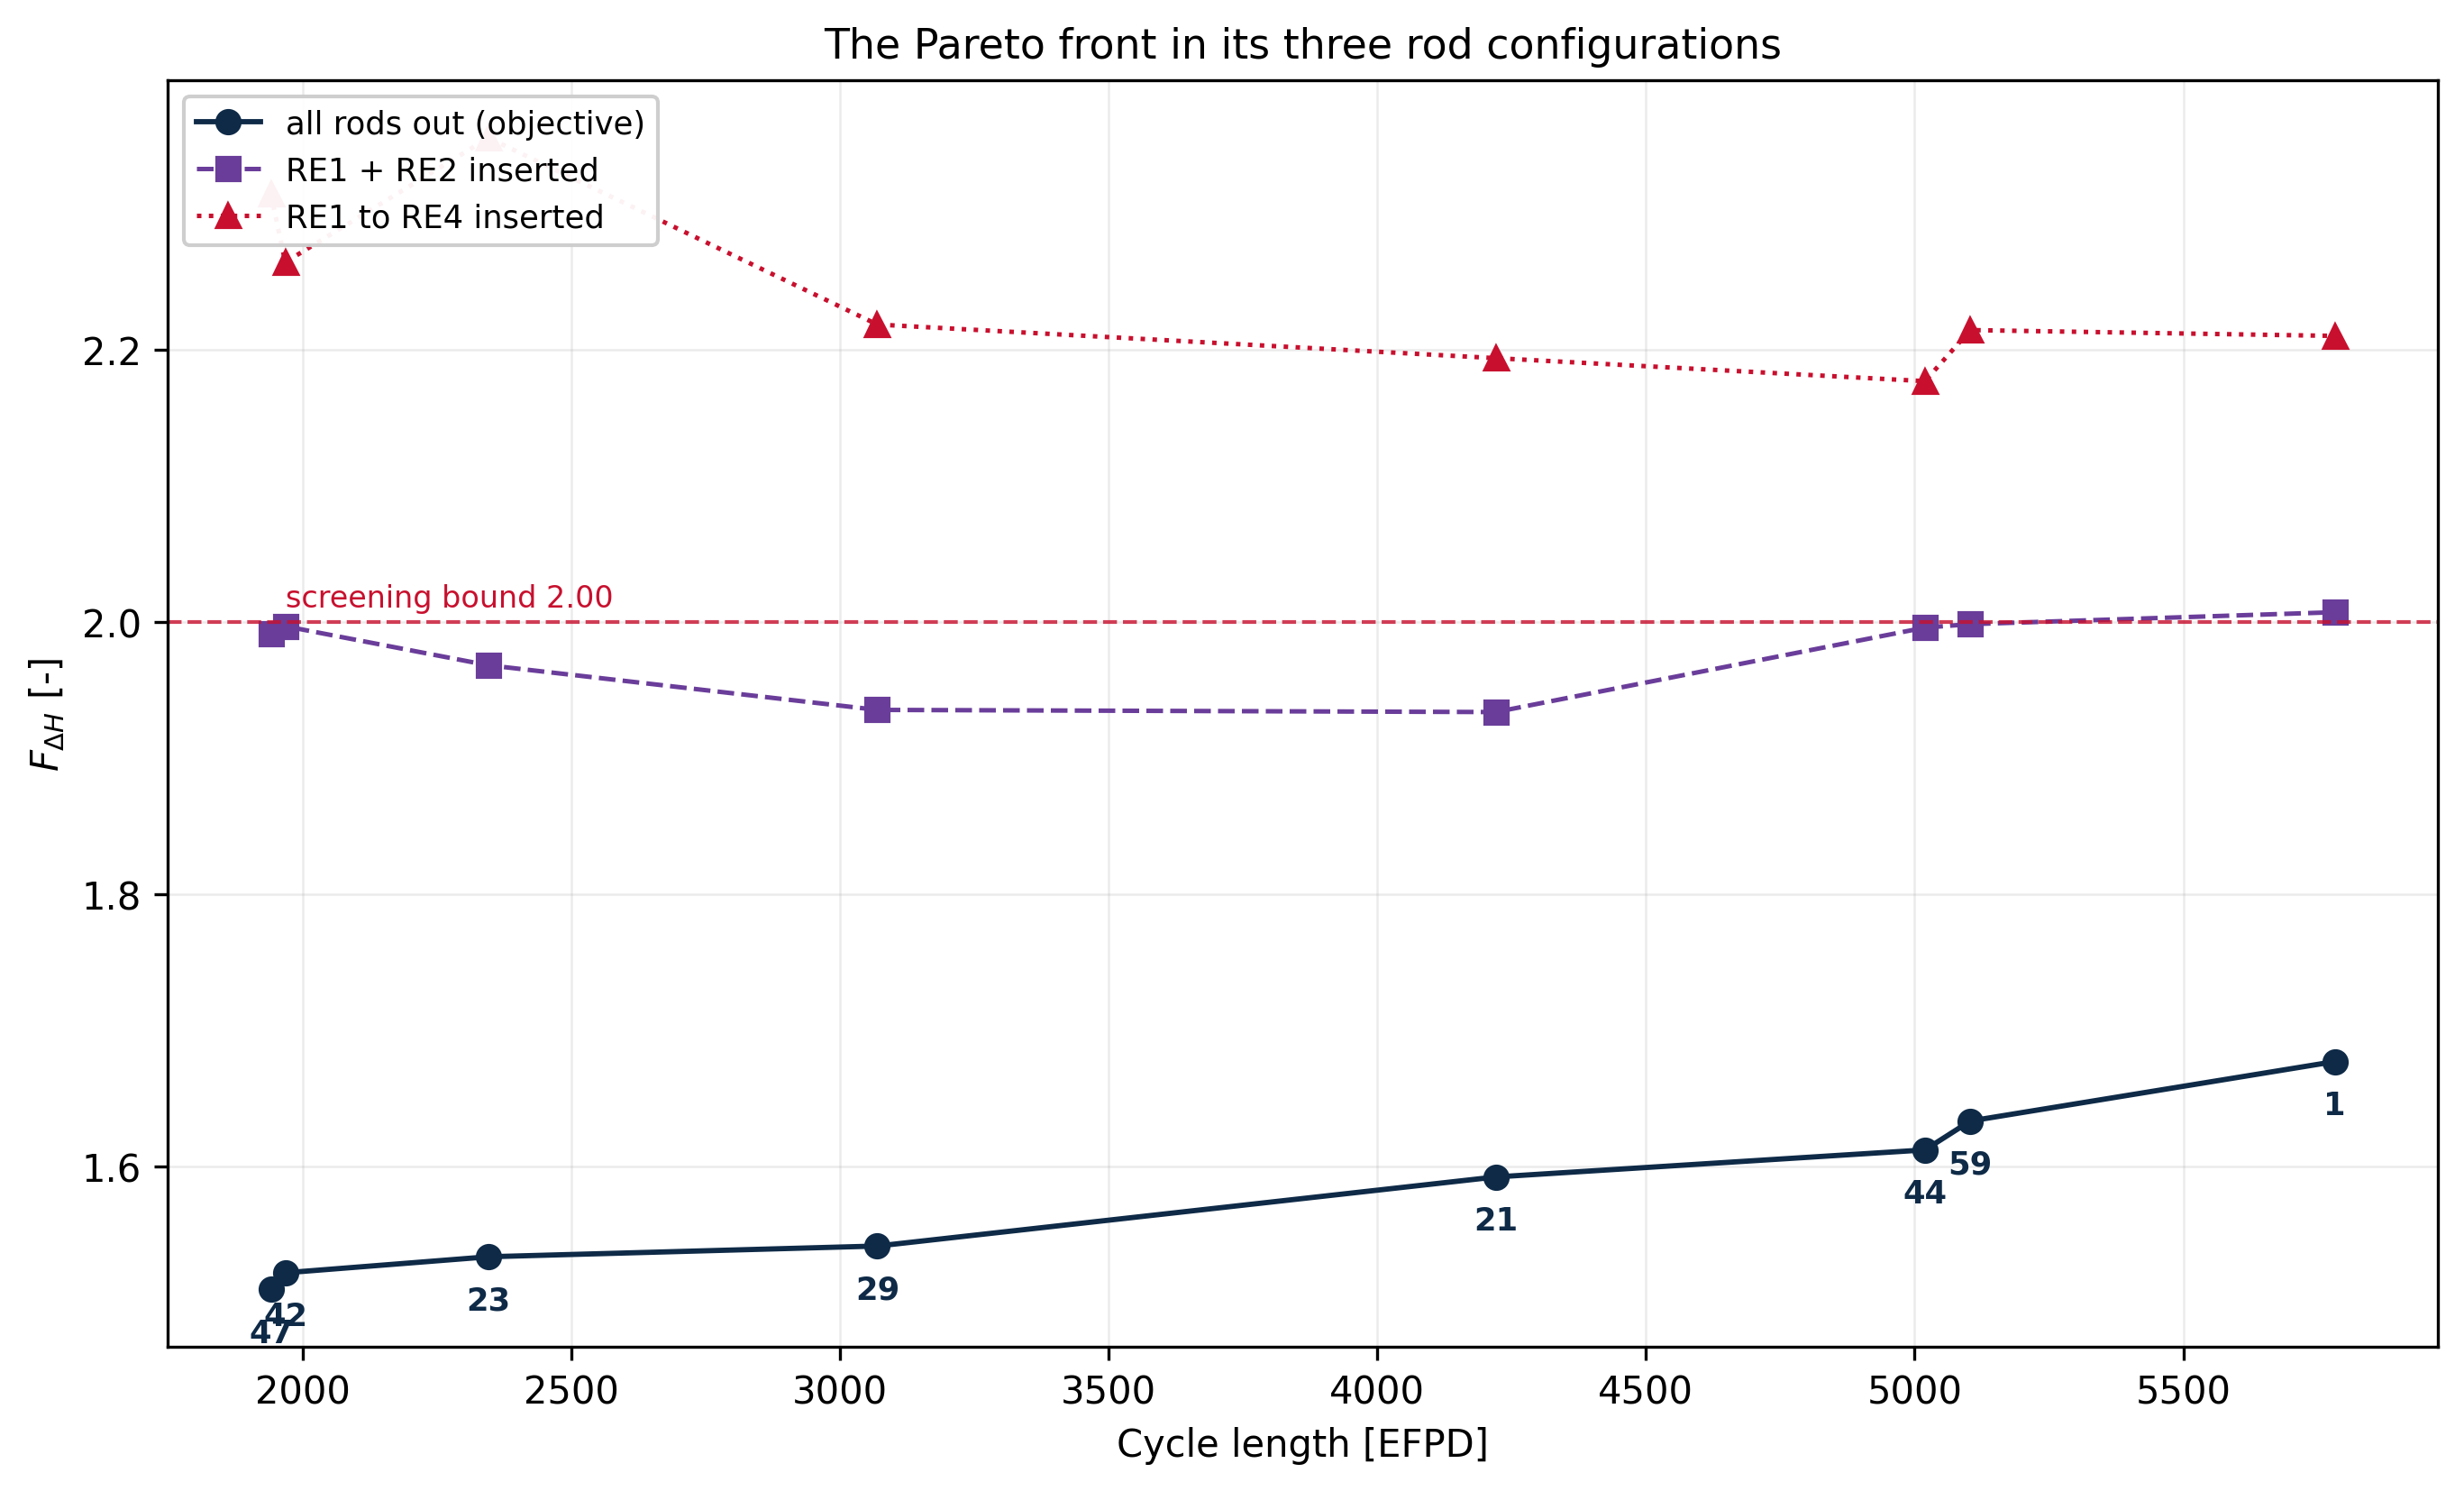
\includegraphics[width=0.95\linewidth]{images/c8_front_split}
  \caption{The Campaign 8 front in its three rod configurations.}
  \label{fig:c8-split}
\end{figure}

% ---------------------------------------------------------------------
%  Validation of the framework on the Campaign 8 archive.
%  Protocol in Section \ref{sec:validation-framework}.
%  Tables generated by c8_surrogate_cv.py (c8_cv_table.tex) and
%  c8_front_stability.py (c8_stab_table.tex).
% ---------------------------------------------------------------------

\subsection{Cross-validation of the surrogate}
\label{sec:res-c8-cv}

The protocol of Section~\ref{sec:validation-surrogate} is applied to the
60 archived designs. Table~\ref{tab:c8-cv-loo} and
Figure~\ref{fig:c8-cv-loo} report the leave-one-out
result for the two objectives and for the two eigenvalues that carry the
controllability screen of Section~\ref{sec:meth-ctrl}. The exercise is a
post-processing step on the archive and costs no transport time.

\begin{table}[htbp]
  \centering
  \small
  \setlength{\tabcolsep}{4.5pt}
  \begin{threeparttable}
  \caption[Leave-one-out validation of the surrogate]{Leave-one-out cross-validation of the Gaussian Process surrogate on the Campaign 8 archive.}
  \label{tab:c8-cv-loo}
  \begin{tabular}{llrrrrrrr}
    \toprule
    Quantity & Subset & $n$ & RMSE & $R^2$ & $\rho_\mathrm{S}$ & Cov.\ $1\sigma$ & Cov.\ $2\sigma$ & $s_z$ \\
    \midrule
    Cycle length [EFPD] & all & 60 & 220 & 0.988 & 0.997 & 0.77 & 0.87 & 1.63 \\
     & feasible & 19 & 145 & 0.990 & 0.988 & 0.74 & 0.89 & 1.81 \\
    $F_{\Delta H}$ & all & 60 & 0.0287 & 0.690 & 0.830 & 0.65 & 0.93 & 1.26 \\
     & feasible & 19 & 0.0227 & 0.829 & 0.900 & 0.63 & 0.89 & 1.26 \\
    $k_\mathrm{core}$ & all & 60 & 0.0151 & 0.978 & 0.967 & 0.67 & 0.97 & 1.11 \\
     & feasible & 19 & 0.0111 & 0.930 & 0.875 & 0.63 & 1.00 & 0.98 \\
    $k_\mathrm{RE}$ & all & 60 & 0.0110 & 0.985 & 0.961 & 0.65 & 0.97 & 1.11 \\
     & feasible & 19 & 0.0081 & 0.959 & 0.923 & 0.68 & 1.00 & 1.02 \\
    \bottomrule
  \end{tabular}
  \begin{tablenotes}\footnotesize
    \item RMSE is the root mean square error of the held-out prediction. $R^2$ is the coefficient of determination. $\rho_\mathrm{S}$ is the Spearman rank correlation between predicted and true values. Cov.\ $1\sigma$ and Cov.\ $2\sigma$ are the fractions of true values inside the one-sigma and two-sigma predictive intervals, with nominal values 0.683 and 0.954. $s_z$ is the standard deviation of the standardised residual, equal to 1 for a calibrated predictor.
    \item Source: c8\_surrogate\_cv.py on the archive of 60 designs, of which 19 are feasible.
  \end{tablenotes}
  \end{threeparttable}
\end{table}

Four readings follow directly from the table.

\begin{enumerate}
  \item The cycle length is the best predicted quantity. Its coefficient
        of determination is 0.988 over the archive and 0.990 over the
        feasible subset, and the held-out root mean square error falls
        from 220 to 145 EFPD when the fit is scored on the feasible
        designs alone.

  \item The peaking factor is the worst predicted quantity. Its
        coefficient of determination is 0.690 over the archive and 0.829
        over the feasible subset. The held-out root mean square error of
        0.0287 over the archive is of the same order as the spacing of
        the front members of Table~\ref{tab:c8-front}, whose adjacent
        designs differ by 0.008 to 0.051 in $F_{\Delta H}$.

  \item The two eigenvalues are predicted to 0.0151 and 0.0110 in $k$
        over the archive, that is \num{1510} and \SI{1100}{pcm} read as
        $10^{5}\,\Delta k$. Their rank correlations, 0.967 and 0.961,
        are the quantity the acquisition actually uses, because the
        margin rule of Section~\ref{sec:meth-acq} ranks candidates
        rather than reading their absolute values.

  \item The predictive intervals are too narrow on the objectives and
        close to correct on the eigenvalues. The one-sigma coverage lies
        between 0.63 and 0.77 against a nominal 0.683, and the
        standardised residual has a standard deviation of 1.63 and 1.81
        on the cycle length, against 1 for a calibrated predictor. The
        two eigenvalues have $s_z$ between 0.98 and 1.11.
\end{enumerate}

\begin{figure}[htbp]
  \centering
  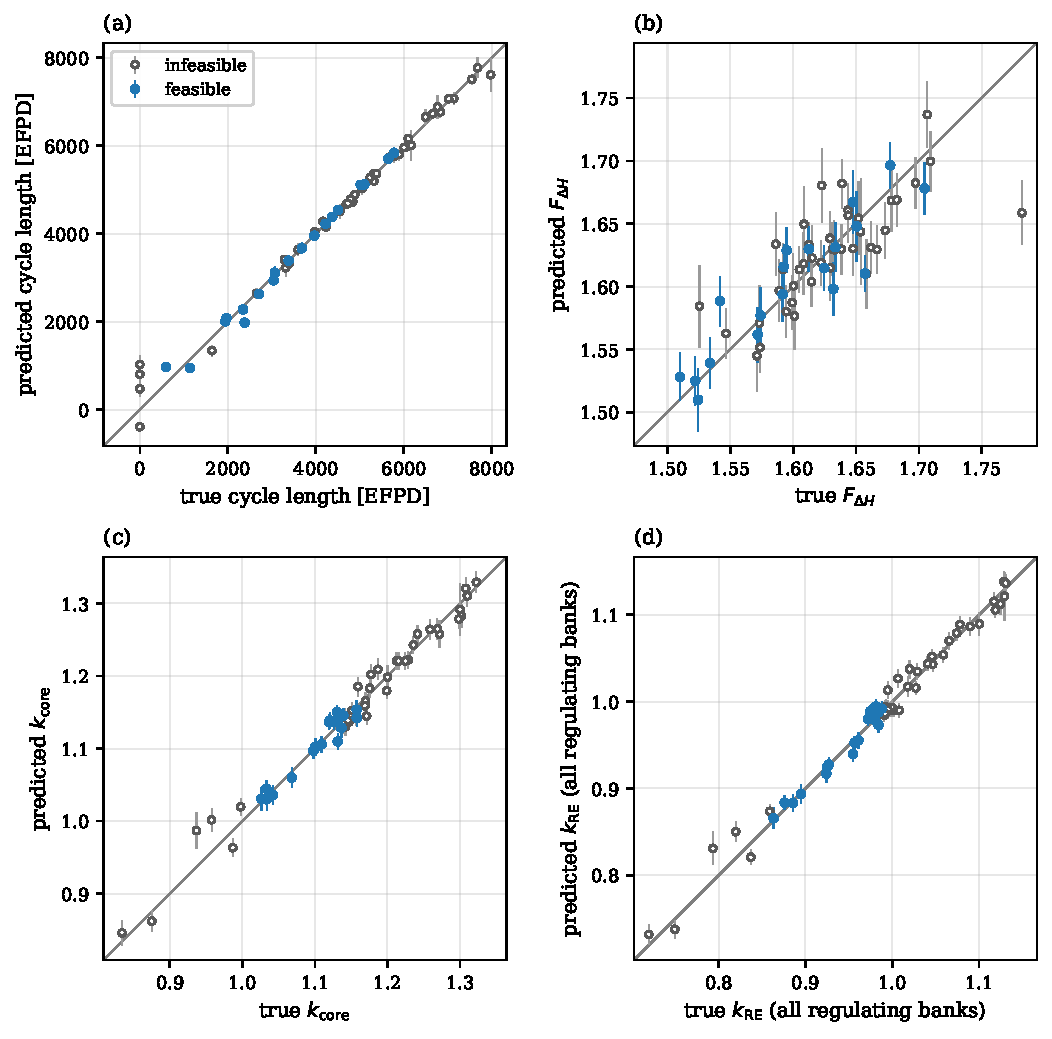
\includegraphics[width=\linewidth]{images/c8_cv_loo}
  \caption[Leave-one-out predictions against transport truth]{Held-out
  prediction against transport truth for the two objectives and the two
  eigenvalues of the controllability screen. Error bars are one
  predictive standard deviation.}
  \label{fig:c8-cv-loo}
\end{figure}

Figure~\ref{fig:c8-cv-loo} shows where the residuals of
Table~\ref{tab:c8-cv-loo} sit. The two eigenvalues and the cycle length
follow the diagonal over their whole range. The exception is the
short-cycle end of the archive, where the held-out prediction departs
from the truth by several hundred effective full-power days and is
negative for one design, since a Gaussian Process is not constrained to
return non-negative outputs. Those designs are the ones that never reach
the reactivity target and are rejected long before the front is formed.

The leave-one-out result measures the surrogate at the end of the
campaign. The walk-forward result of
Figure~\ref{fig:c8-cv-walkforward} measures it at decision time, on the
six designs of each infill block, with the surrogate fitted only on the
evaluations that preceded the block.

\begin{figure}[htbp]
  \centering
  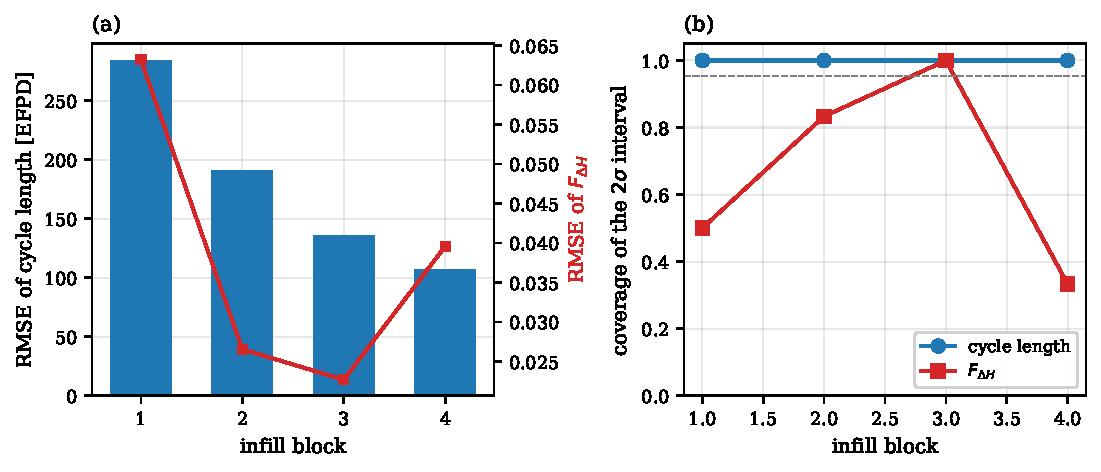
\includegraphics[width=\linewidth]{images/c8_cv_walkforward}
  \caption[Walk-forward accuracy and coverage per infill block]{Block
  root mean square error and two-sigma coverage of the surrogate at
  decision time, per infill block. The dashed line in panel (b) is the
  nominal coverage of 0.954.}
  \label{fig:c8-cv-walkforward}
\end{figure}

Three readings follow from the walk-forward record.

\begin{enumerate}
  \item The cycle-length prediction improved monotonically as the
        archive grew. The block root mean square error fell from
        \SI{285}{EFPD} at infill block 1 to \num{191}, \num{136} and
        \SI{107}{EFPD} at blocks 2, 3 and 4.

  \item The peaking prediction did not. Its block root mean square error
        fell from 0.063 to 0.027 and 0.022 at blocks 2 and 3, and then
        rose to 0.040 at block 4.

  \item At decision time the intervals are conservative on the cycle
        length and erratic on the peaking factor. The two-sigma coverage
        of the cycle length is 1.00 at every block, above the nominal
        0.954, while that of the peaking factor is 0.50, 0.83, 1.00 and
        0.33. Each block holds six designs, so the coverage is quantised
        in steps of one sixth and these four values carry little
        resolution.
\end{enumerate}

The walk-forward surrogate is fitted on fewer designs than the
leave-one-out surrogate and therefore returns wider predictive
intervals. This is why the cycle length appears over-confident in
Table~\ref{tab:c8-cv-loo}, with a two-sigma coverage of 0.87, and
under-confident in Figure~\ref{fig:c8-cv-walkforward}, with a coverage
of 1.00. The two measurements are not in conflict, because they score
different fits.

An over-confident cycle-length surrogate has no direct effect on the
feasibility margin of the acquisition, because the margin rule of
Section~\ref{sec:meth-acq} acts on the constraint surrogates and the
cycle length is an objective. The constraint eigenvalues
$k_\mathrm{core}$ and $k_\mathrm{RE}$ are the quantities whose
predictive standard deviations are multiplied by $\kappa$, and their
two-sigma coverage in Table~\ref{tab:c8-cv-loo} is 0.97 to 1.00, at or
above the nominal value, so the margin added during the campaign was
at least as wide as intended. The under-stated cycle-length
uncertainty enters only the uncertainty ranking of the candidates,
where a narrower band on that output gives the objective slightly
less weight in the choice of the infill batch.

\subsection{Stability of the front}
\label{sec:res-c8-stability}

The protocol of Section~\ref{sec:validation-front} is applied to the
eight members of Table~\ref{tab:c8-front}.
Table~\ref{tab:c8-front-stability} reports, for each member, the
evaluation at which it entered the feasible non-dominated set, its
exclusive hypervolume contribution and its probability of remaining
non-dominated under the Monte Carlo noise of the transport solves.

\begin{table}[htbp]
  \centering
  \begin{threeparttable}
  \caption[Stability of the Campaign 8 front]{Entry, exclusive hypervolume contribution and noise robustness of the Campaign 8 front members.}
  \label{tab:c8-front-stability}
  \begin{tabular}{rrrrrr}
    \toprule
    Design & Cycle [EFPD] & $F_{\Delta H}$ & Entered at & Excl.\ HV [\%] & $P$(front) \\
    \midrule
    47 & 1941 & 1.5099 & 48 & 0.1 & 0.80 \\
    42 & 1968 & 1.5221 & 43 & 0.0 & 0.73 \\
    23 & 2346 & 1.5338 & 24 & 0.1 & 0.73 \\
    29 & 3070 & 1.5417 & 30 & 1.8 & 1.00 \\
    21 & 4221 & 1.5925 & 22 & 1.1 & 0.92 \\
    44 & 5019 & 1.6123 & 45 & 0.8 & 0.94 \\
    59 & 5104 & 1.6335 & 60 & 0.2 & 0.99 \\
    1 & 5782 & 1.6772 & 2 & 14.0 & 1.00 \\
    \bottomrule
  \end{tabular}
  \begin{tablenotes}\footnotesize
    \item Entered at is the evaluation count at which the design first became a member of the feasible non-dominated set and it was never displaced afterwards. Excl.\ HV is the hypervolume lost when the design alone is removed, as a percentage of the front hypervolume at the campaign reference point. $P$(front) is the probability that the design remains non-dominated when the objectives of every feasible design are perturbed by Gaussian Monte Carlo noise, with $\sigma_k = 44$\,pcm propagated to the cycle length and $\sigma_F = 0.01$ on $F_{\Delta H}$, over 5000 replicates.
  \end{tablenotes}
  \end{threeparttable}
\end{table}

Three readings follow directly from the table.

\begin{enumerate}
  \item The front was still growing when the campaign stopped. Design 59
        entered at evaluation 60, the last of the campaign, and no
        member was displaced afterwards. The hypervolume record of
        Section~\ref{sec:res-c8-blocks} reaches the same conclusion from
        a different quantity, namely that the campaign is one block
        short of a formal stop.

  \item One design carries the front. Design 1, the long-cycle extreme,
        holds \SI{14.0}{\%} of the front hypervolume exclusively,
        against \SI{1.8}{\%} for design 29 and \SI{1.1}{\%} for design
        21. The three lowest-peaking members, 47, 42 and 23, contribute
        \SI{0.1}{\%}, \SI{0.0}{\%} and \SI{0.1}{\%}, because each is
        nearly covered by its neighbours in the objective plane.

  \item The low-peaking end of the front is not resolved by the
        transport statistics. Under the noise model of
        Equation~\eqref{eq:val-sigma-cycle}, with
        $\sigma_k = \SI{44}{pcm}$ propagated to the cycle length and
        $\sigma_F = 0.01$ on the peaking factor, designs 47, 42 and 23
        remain non-dominated in 0.80, 0.73 and 0.73 of 5000 replicates,
        against 1.00 for designs 29 and 1. This quantifies the
        limitation stated in Section~\ref{sec:res-c8-limits}, that the
        ordering of the three lowest-peaking designs is not resolved.
\end{enumerate}

Figure~\ref{fig:c8-stab-chrono} gives the chronology of the set, with the
block boundaries dotted in panel~(a), and Figure~\ref{fig:c8-stab-robust}
its robustness.

\begin{figure}[htbp]
  \centering
  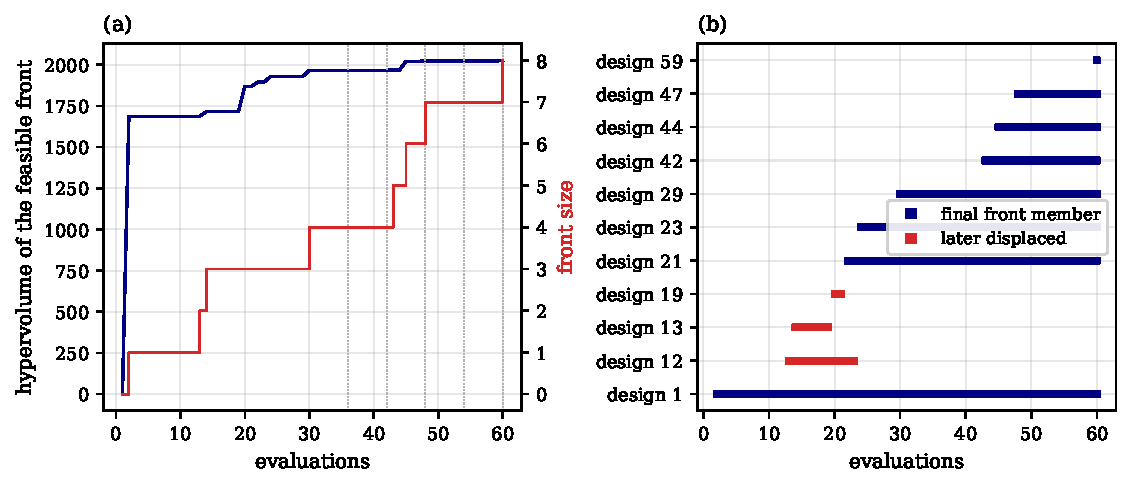
\includegraphics[width=\linewidth]{images/c8_stab_chrono}
  \caption[Chronology of the feasible non-dominated set]{Chronology of the Campaign 8 feasible front: hypervolume, front size and membership interval of every design, in evaluation order.}
  \label{fig:c8-stab-chrono}
\end{figure}

Figure~\ref{fig:c8-stab-chrono} adds the displacement record that
Table~\ref{tab:c8-front-stability} does not carry. Eleven designs
entered the feasible non-dominated set over the campaign and three of
them, designs 12, 13 and 19, were displaced later. All three entered and
left within the design of experiments. The four design of experiments
members that survived, designs 1, 21, 23 and 29, entered at evaluations
2, 22, 24 and 30 and were never displaced. The front size grew from one
member at evaluation 2 to eight at evaluation 60, and the last increment
is the entry of design 59.

\begin{figure}[htbp]
  \centering
  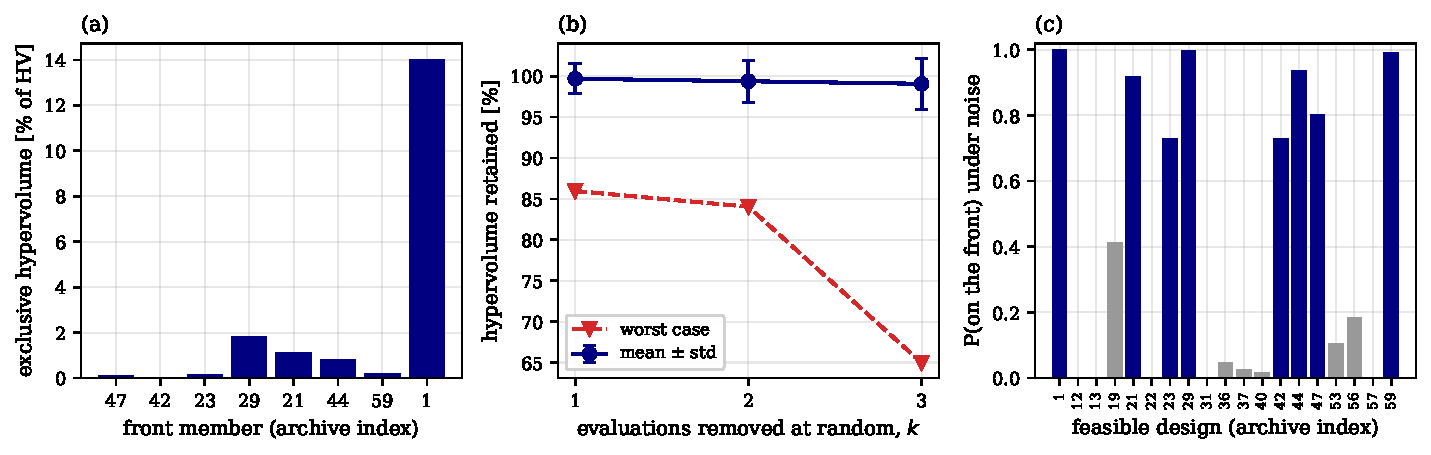
\includegraphics[width=\linewidth]{images/c8_stab_robust}
  \caption[Robustness of the Campaign 8 front]{Exclusive hypervolume of
  each front member, hypervolume retained after the random removal of
  evaluations, and the probability that each feasible design belongs to
  the front under Monte Carlo noise.}
  \label{fig:c8-stab-robust}
\end{figure}

Two further readings follow from Figure~\ref{fig:c8-stab-robust}.

\begin{enumerate}
  \item The front is robust to lost evaluations on average and fragile
        in the worst case. Removing one, two or three evaluations at
        random from the archive retains \SI{99.7}{\%}, \SI{99.4}{\%} and
        \SI{99.1}{\%} of the front hypervolume on average, while the
        worst case retains \SI{86.1}{\%}, \SI{84.2}{\%} and
        \SI{65.0}{\%}. The worst case at one removal is the loss of
        design 1, whose exclusive contribution is \SI{14.0}{\%}.

  \item Three designs that are not front members would become members
        under the same noise with non-negligible probability. Design 19
        reaches 0.41, design 56 reaches 0.19 and design 53 reaches 0.11.
        Design 19 is one of the three that were displaced during the
        design of experiments.
\end{enumerate}

A small exclusive hypervolume contribution and a membership probability
near unity are not in conflict. The first says that the design can be
removed with almost no loss of front hypervolume. The second says that
the design is not displaced by noise. Design 59 is both, with
\SI{0.2}{\%} of exclusive hypervolume and a membership probability of
0.99.

The value $\sigma_F = 0.01$ is assumed rather than measured, so the
three membership probabilities below unity are indicative and scale with
that assumption.

%% AUTHOR: the physical reading of why the low-peaking end of the front
%% is the crowded end, and whether the three statistically equivalent
%% designs should be carried forward as a group or reduced to one.

\subsection{Search against exhaustive enumeration}
\label{sec:res-c8-valgrid}

The second validation exercise of Section~\ref{sec:validation-grid}
compares the surrogate-assisted search against exhaustive enumeration on
the two-variable slice at frozen reflector thickness and frozen
gadolinia rod count. The slice is taken at
$t_\mathrm{refl} = \SI{4.289}{cm}$ and $n_\mathrm{Gd} = 12$, the values
of design 47, so that the enrichment and the gadolinia weight fraction
remain as live variables. Table~\ref{tab:valgrid} reports the
comparison and Figure~\ref{fig:valgrid-objective} places it in the
objective plane.

\begin{table}[htbp]
  \centering
  \begin{threeparttable}
  \caption[Search against exhaustive enumeration]{Surrogate-assisted search against exhaustive enumeration on the two-variable slice.}
  \label{tab:valgrid}
  \begin{tabular}{lrr}
    \toprule
    Quantity & Enumeration & Search \\
    \midrule
    Truth evaluations & 35 & 20 \\
    Feasible designs & 17 & 15 \\
    Front members & 8 & 8 \\
    Hypervolume, nadir reference & 193.1 & 209.7 \\
    Hypervolume ratio & 1 & 1.086 \\
    Union-front members & 3 & 8 \\
    \midrule
    IGD, normalised & \multicolumn{2}{r}{0.137} \\
    GD, normalised & \multicolumn{2}{r}{0.104} \\
    $I_{\varepsilon+}$(search, enumeration), normalised & \multicolumn{2}{r}{0.145} \\
    $I_{\varepsilon+}$ in cycle length [EFPD] & \multicolumn{2}{r}{328} \\
    $I_{\varepsilon+}$ in $F_{\Delta H}$ & \multicolumn{2}{r}{0.0199} \\
    Enumerated-front coverage, strict / within 0.02 & \multicolumn{2}{r}{0.62 / 0.75} \\
    Wall-clock [h] & 8.5 & 4.9 \\
    \bottomrule
  \end{tabular}
  \begin{tablenotes}\footnotesize
    \item Objectives are normalised by the range of the union of the two fronts before the distance indicators are computed. IGD is the inverted generational distance from the enumerated front to the recovered front. GD is the generational distance from the recovered front to the enumerated front. $I_{\varepsilon+}$ is the additive epsilon indicator, the smallest shift that makes the recovered front weakly dominate every enumerated-front point. The hypervolume reference point is the nadir of the union of the two fronts plus ten per cent of the range.
    \item Slice: $t_\mathrm{refl} = \SI{4.28885}{cm}$, $n_\mathrm{Gd} = 12$. Source: valgrid\_compare.py.
  \end{tablenotes}
  \end{threeparttable}
\end{table}

\begin{figure}[htbp]
  \centering
  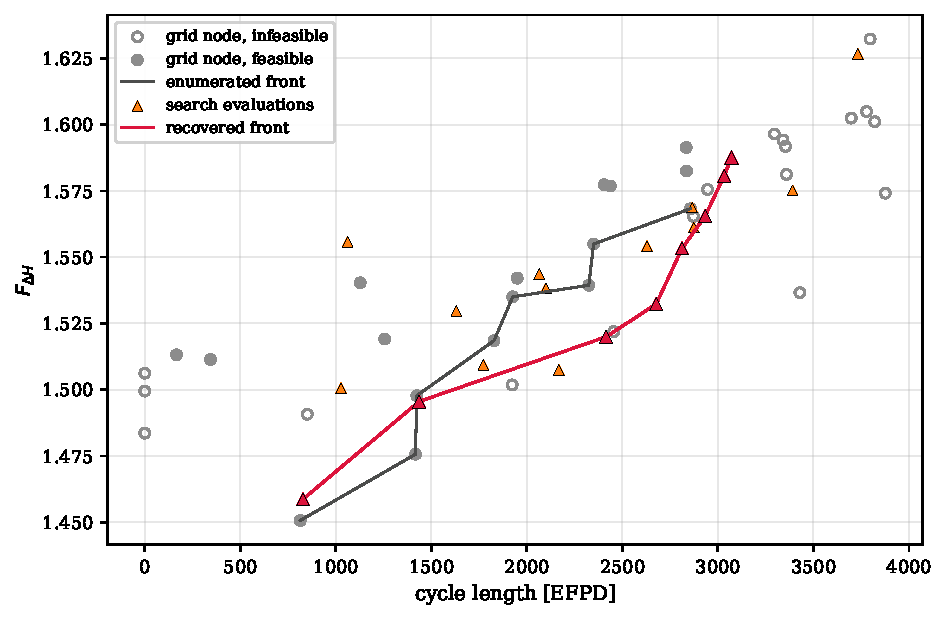
\includegraphics[width=0.92\linewidth]{images/valgrid_objective}
  \caption[Enumerated and recovered fronts in the objective
  plane]{Objective plane of the two-variable slice, with the 35
  enumerated grid nodes, the 20 search evaluations and the two feasible
  non-dominated sets.}
  \label{fig:valgrid-objective}
\end{figure}

Four readings follow from the table and from
Figure~\ref{fig:valgrid-objective}.

\begin{enumerate}
  \item The search recovered a front of the same size at a lower cost.
        Both fronts hold eight members. The search used 20 truth
        evaluations against 35, that is \SI{57}{\%} of the count, and
        \SI{4.9}{h} of wall clock against \SI{8.5}{h}, that is
        \SI{58}{\%} of the time.

  \item The recovered front has the larger hypervolume, 209.7 against
        193.1, a ratio of 1.086. Section~\ref{sec:validation-grid}
        anticipates a ratio above one, because the search places designs
        anywhere in the box while the enumeration is confined to grid
        nodes.

  \item The recovered front dominates most of the enumerated front. The
        union of the two fronts retains all eight recovered members and
        only three of the eight enumerated members, so five enumerated
        members are dominated outright. The strict coverage of 0.62
        rises to 0.75 when a tolerance of 0.02 in the normalised
        objectives is allowed.

  \item The domination is not complete. The additive epsilon indicator
        is 0.145 in the normalised space, equivalent to \SI{328}{EFPD}
        on the cycle length or to 0.0199 on the peaking factor. The
        binding point is on the short-cycle portion of the enumerated
        front, near \SI{1420}{EFPD}, where the recovered front sits
        about 0.02 higher in $F_{\Delta H}$.
\end{enumerate}

The acquisition also spent its evaluations better. Of the 35 enumerated
nodes 17 are feasible, \SI{48.6}{\%}, against 15 of the 20 search
evaluations, \SI{75.0}{\%}. Figure~\ref{fig:valgrid-design} shows the
same comparison in the design plane.

\begin{figure}[htbp]
  \centering
  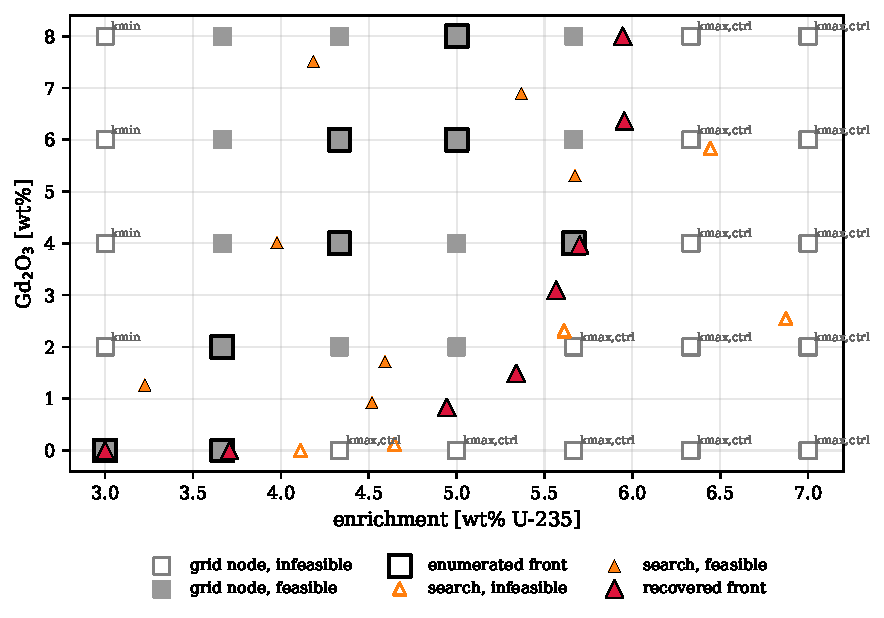
\includegraphics[width=0.92\linewidth]{images/valgrid_design}
  \caption[The two fronts in the design plane of the slice]{Design plane
  of the two-variable slice. Infeasible grid nodes are annotated with
  the constraint they violate.}
  \label{fig:valgrid-design}
\end{figure}

Figure~\ref{fig:valgrid-design} shows where the two fronts sit in the
design plane, and it answers where the difference of \SI{8.6}{\%} in
hypervolume comes from.

The feasible band of the slice is bounded on both sides by a reactivity
constraint. The nodes at \SI{3.0}{wt\%} enrichment with gadolinia at or
above \SI{2}{wt\%} fail the lower reactivity bound $k_\mathrm{min}$. The
nodes at \SI{6.33}{wt\%} and above, together with the unpoisoned nodes
from \SI{4.33}{wt\%} upward, fail the controllability screen. No node in
the slice fails on peaking.

The enumerated front is confined to the five gadolinia values of the
grid, 0, 2, 4, 6 and \SI{8}{wt\%}. The recovered front places three of
its eight members between 0 and \SI{2}{wt\%}, at 0.8, 1.45 and
\SI{3.05}{wt\%} with enrichments of 4.95, 5.35 and \SI{5.57}{wt\%},
inside a band that the grid does not sample. It also reaches
\SI{5.95}{wt\%} enrichment, beyond the last feasible grid column at
\SI{5.67}{wt\%}, and therefore extends the front to \SI{3070}{EFPD}
against \SI{2840}{EFPD} for the enumeration.

Figure~\ref{fig:valgrid-surrogate} tests the surrogate on the grid nodes
it has not seen.

\begin{figure}[htbp]
  \centering
  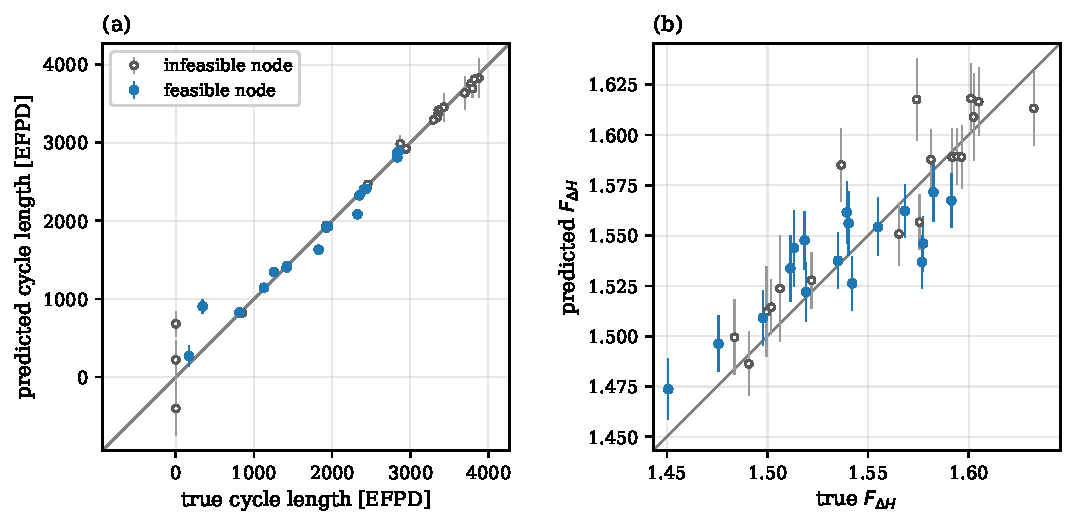
\includegraphics[width=\linewidth]{images/valgrid_surrogate}
  \caption[Surrogate prediction at the unseen grid nodes]{Surrogate prediction at the 35 unseen grid nodes. Error bars are one predictive standard deviation.}
  \label{fig:valgrid-surrogate}
\end{figure}

The last check of Section~\ref{sec:validation-grid} is a pure
extrapolation test. The surrogate fitted on the 20 search evaluations is
evaluated at all 35 grid nodes, none of which entered its training set.
Figure~\ref{fig:valgrid-surrogate} gives the result. The cycle length
follows the diagonal over the whole range, with the same departure at
the short-cycle end already seen in Figure~\ref{fig:c8-cv-loo}. The
peaking factor scatters more widely, and the one-sigma bars of most
nodes intersect the diagonal.

Two limits bound this exercise. The slice is two-dimensional, so it
tests the search on a problem an order of magnitude smaller than the
four-variable campaign, and the enumeration grid is coarse in gadolinia,
which is the very axis on which the recovered front gains its
hypervolume.

%% AUTHOR: two or three sentences of physics on why the low-gadolinia,
%% high-enrichment corridor of Figure~\ref{fig:valgrid-design} is the
%% one that carries the front, and on whether the same corridor is
%% visible in the full four-variable archive of
%% Section~\ref{sec:res-c8-front}.

%% AUTHOR: one sentence on whether an 8.6 per cent hypervolume gain at
%% 57 per cent of the evaluations is the claim you want to make for the
%% framework, or whether the epsilon indicator of 328 EFPD is the more
%% conservative headline.


\subsection{The two-bank subset}
\label{sec:res-c8-split}

Table~\ref{tab:c8-two} lists the four feasible designs that the first
two banks alone hold subcritical at the margin. Design 12 is included
for completeness and is not a candidate. The four designs occupy the
narrow reactivity window of Equation~\eqref{eq:two-bank-ceiling}, with
unrodded eigenvalues between 1.026 and 1.042, and none of them is on
the front, because the front is defined by cycle length and they carry
a beginning-of-life excess of only \num{2564} to \SI{4068}{pcm}.

\begin{table}[htbp]
  \centering
  \small
  \caption[The Campaign 8 two-bank subset]{Feasible Campaign 8 designs controllable with the first two banks. Columns as in Table~\ref{tab:c8-front}.}
  \label{tab:c8-two}
  \setlength{\tabcolsep}{3.8pt}
  \begin{tabular}{cccccccccc}
    \toprule
    Design & EFPD & rings & $w_\mathrm{Gd}$ & $n_\mathrm{Gd}$ &
      $t_\mathrm{refl}$ & $k^\mathrm{core}$ & excess & $F$ & $F_{2}$ \\
    {[--]} & [d] & [wt\%] & [wt\%] & [rods] & [cm] & [--] & [pcm] &
      [--] & [--] \\
    \midrule
    53 & 1142 & 2.48, 3.08, 3.97 & 2.92 & 12 & 4.74 & 1.026 & 2564 & 1.524 & 2.020 \\
    13 & 2383 & 3.70, 4.59, 5.91 & 5.25 & 24 & 3.15 & 1.042 & 4068 & 1.632 & 2.131 \\
    31 & 3381 & 4.74, 5.89, 7.58 & 3.38 & 40 & 4.18 & 1.034 & 3282 & 1.650 & 2.074 \\
    12 &  598 & 3.47, 4.30, 5.54 & 7.06 & 20 & 2.46 & 1.033 & 3207 & 1.592 & 2.061 \\
    \bottomrule
  \end{tabular}
\end{table}

The subset is where the operating physics of a pressurised water
reactor is recognisable. A commercial core at hot full power holds its
beginning-of-life excess with soluble boron and burnable absorber and
keeps the regulating banks nearly withdrawn, so that the rods carry
only the power defect and the manoeuvring band. The eight front
designs would need the four regulating banks inserted deep enough to
hold \num{8930} to \SI{13627}{pcm} at power with \SI{1000}{ppm} in the
coolant, which no pressurised water reactor does, and which would
impose the rodded peaking of Figure~\ref{fig:c8-split} continuously.
The two-bank designs hold \num{2564} to \SI{4068}{pcm}, of the order
that boron adjustment alone can carry.

The comparison with a licensed-class core makes the point
quantitative. The NuScale-like benchmark on which the fuel design of
this thesis rests reports, at beginning of life with \SI{1000}{ppm} of
soluble boron, a fuel temperature of \SI{900}{K} and a coolant
temperature of \SI{600}{K}, a reference all-rods-out eigenvalue of
$1.02768 \pm 0.00001$~\cite{fridman_nuscale_benchmark_2023}, which an
OpenMC model with ENDF/B-VII.1 reproduces within 16 to
\SI{31}{pcm}~\cite{ez_aldeen_2025}.
Its sixteen control rod assemblies, in four banks of four, are worth
\num{1965}, \num{2379}, \num{3727} and \SI{3728}{pcm} individually and
\SI{19231}{pcm} all together. The regulating requirement of that core
at beginning of life is therefore below \SI{2800}{pcm}, held by one
bank with margin, and the shutdown banks are reserved.
Table~\ref{tab:bench-compare} places the two Campaign 8 candidate
lists against it. The worth column is for sixteen control rod
assemblies in every case, namely the four banks of the benchmark
together and the four regulating banks of this core.

\begin{table}[htbp]
  \centering
  \small
  \caption[Reactivity to be held by the rods, against the
  benchmark]{Beginning-of-life reactivity to be held by the rods at \SI{1000}{ppm}: NuScale-like benchmark and the two Campaign 8 candidate lists.}
  \label{tab:bench-compare}
  \begin{tabularx}{\textwidth}{@{}>{\raggedright\arraybackslash}X ccc@{}}
    \toprule
    Core & $k_\mathrm{eff}^\mathrm{core}$ & excess to hold &
      worth of 16 CRA \\
     & [--] & [pcm] & [pcm] \\
    \midrule
    NuScale-like benchmark~\cite{fridman_nuscale_benchmark_2023}
      & 1.028 & 2700 & 19231 \\
    Campaign 8 front, Table~\ref{tab:c8-front}
      & 1.098 to 1.158 & 8930 to 13627 & 14270 to 17665 \\
    Campaign 8 two-bank subset, Table~\ref{tab:c8-two}
      & 1.026 to 1.042 & 2564 to 4068 & 13906 to 16303 \\
    \bottomrule
  \end{tabularx}
\end{table}

The rods are alike. Sixteen assemblies of this core are worth
\num{11466} to \SI{19313}{pcm} across the archive, the same range as
the sixteen of the benchmark, because the rod design, the absorber
densities and the guide-tube geometry are the benchmark's. What
differs is how much the rods are asked to hold. The two-bank subset
sits in the regime of the benchmark. The front asks three to five
times what a licensed-class small core asks of its rods at start-up,
and it can only be held with the four regulating banks inserted deep
at power.


The two requirements pull in opposite directions because a longer
cycle is bought with reactivity that is burned later, and that
reactivity must be held at the start of life. With the soluble boron
and the gadolinia already present in every eigenvalue of this work,
whatever the burnup has not yet consumed is held by the rods, so the
excess that lengthens the cycle is the same excess that drives the
regulating banks into the core. The consequence for the formulation is
drawn in Section~\ref{sec:concl-reform}: the cycle length becomes a
constraint at the required value and the two-bank eigenvalue an
objective. That is a stronger use of the two-bank reading than a
constraint would be, since a constraint would only bound the margin
whereas an objective maximises it.


\subsection{Burnup and composition dependence of the leakage
correction}
\label{sec:res-kt-burnup}

The leakage-corrected target of Equation~\eqref{eq:ktarget} rests on
two assumptions that the closure check of
Section~\ref{sec:res-corevalidation} does not reach. The leakage
factor is evaluated once, at beginning of life, on a single reference
composition of \num{4.55} and \SI{4.05}{\percent} by weight without
gadolinia, and it is then held constant over the whole cycle and
applied to every design in the space. Both assumptions are tested
here, on the eight front designs of Table~\ref{tab:c8-front} and on
the two-bank representatives of Table~\ref{tab:c8-two}.

For each design the reflective assembly is depleted once, in a single
shot with the campaign schedule, up to two steps beyond its end of
cycle. At beginning of life and at the two depletion steps that
bracket the end of cycle, the depleted composition is loaded uniformly
into all \num{32} assemblies of the core model of
Section~\ref{sec:meth-ktarget} and into the reflective assembly, and
both eigenvalues are solved with three independent seeds. The measured
leakage factor follows.

\begin{equation}
\mathrm{LF}(B) =
\frac{k_\infty^\mathrm{assembly}(B)}{k_\mathrm{eff}^\mathrm{core}(B)}
\; L_\mathrm{ax}
\label{eq:kt-lf}
\end{equation}

\noindent where the symbols have the following meaning.

\begin{itemize}
  \item $\mathrm{LF}(B)$ is the leakage factor measured at burnup $B$
        on the design's own depleted composition, dimensionless.

  \item $k_\infty^\mathrm{assembly}(B)$ is the infinite multiplication
        factor of the reflective assembly at burnup $B$,
        dimensionless.

  \item $k_\mathrm{eff}^\mathrm{core}(B)$ is the effective
        multiplication factor of the \num{32}-assembly core built with
        the same reflector thickness, loaded uniformly with the same
        depleted composition and closed by a vacuum radial boundary,
        dimensionless.

  \item $L_\mathrm{ax}$ is the axial leakage factor of
        Section~\ref{sec:meth-lax}, equal to \num{1.0289},
        dimensionless.

  \item $B$ is the burnup, in MWd/kgHM.
\end{itemize}

Two quantities are read from the measurement. The drift is the change
of the leakage factor between the two ends of the cycle and tests the
burnup assumption. The residual is the leakage factor minus the
tabulated target and tests the composition assumption. The residual at
the end of cycle is the one that moves the reported cycle length,
through the local reactivity slope of the assembly.

\begin{equation}
\Delta\mathrm{EFPD} =
\frac{\mathrm{LF}(B_\mathrm{EOC}) - k_\mathrm{target}}
     {\left. \mathrm{d}k_\infty / \mathrm{d}B \right|_{B_\mathrm{EOC}}}
\; \frac{1000}{q}
\label{eq:kt-defpd}
\end{equation}

\noindent where the symbols have the following meaning.

\begin{itemize}
  \item $\Delta\mathrm{EFPD}$ is the correction to the reported cycle
        length, in effective full-power days.

  \item $\mathrm{LF}(B_\mathrm{EOC})$ is the leakage factor of
        Equation~\eqref{eq:kt-lf} at the end-of-cycle burnup,
        dimensionless.

  \item $k_\mathrm{target}$ is the tabulated target the optimiser used
        for that design, dimensionless.

  \item $\mathrm{d}k_\infty / \mathrm{d}B$ is the local reactivity
        slope of the assembly between the two bracketing depletion
        steps, in (MWd/kgHM)$^{-1}$, negative at the end of cycle.

  \item $q$ is the core specific power, equal to
        \SI{9.9834}{\watt\per\gram} of heavy metal
        (Table~\ref{tab:model-operating}).

  \item $B_\mathrm{EOC}$ is the end-of-cycle burnup, in MWd/kgHM.
\end{itemize}

Table~\ref{tab:kt-burnup} reports the measurement. Every design ended
its cycle on the reactivity crossing, so no entry is set by the burnup
cap.

\begin{table}[htbp]
  \centering
  \small
  \caption[Burnup dependence of the Route B leakage factor]{Burnup
  dependence of the Route B leakage factor on the Campaign 8 designs.}
  \label{tab:kt-burnup}
  \setlength{\tabcolsep}{4.2pt}
  \begin{tabular}{ccccccccc}
    \toprule
    Design & $e$ & $t_\mathrm{refl}$ & $B_\mathrm{EOC}$ &
      $k_\mathrm{target}$ & $\mathrm{LF}_\mathrm{BOL}$ &
      $r_\mathrm{BOL}$ & drift & $\Delta\mathrm{EFPD}$ \\
    {[--]} & [wt\%] & [cm] & [MWd/kgHM] & [--] & [--] & [pcm] & [pcm] &
      [d] \\
    \midrule
     1 & 11.03 & 3.94 & 57.8 & 1.0829 & 1.0793 & $-329$ & $+33 \pm 126$ & $+56$ \\
    59 &  9.34 & 5.66 & 50.2 & 1.0820 & 1.0796 & $-220$ & $ -4 \pm 107$ & $+43$ \\
    44 &  9.23 & 5.33 & 49.8 & 1.0822 & 1.0798 & $-219$ & $-10 \pm  90$ & $+42$ \\
    21 &  7.81 & 4.92 & 42.3 & 1.0824 & 1.0800 & $-222$ & $+149 \pm 84$ & $+11$ \\
    31 &  6.59 & 4.18 & 33.4 & 1.0828 & 1.0819 & $ -85$ & $-10 \pm  85$ & $+14$ \\
    29 &  5.90 & 4.69 & 31.0 & 1.0825 & 1.0824 & $  -9$ & $-152 \pm 99$ & $+25$ \\
    23 &  4.94 & 4.81 & 23.7 & 1.0824 & 1.0830 & $ +53$ & $-67 \pm 116$ & $ +2$ \\
    42 &  4.44 & 3.76 & 19.7 & 1.0830 & 1.0836 & $ +54$ & $-22 \pm  82$ & $ -4$ \\
    47 &  4.39 & 4.29 & 19.5 & 1.0827 & 1.0830 & $ +27$ & $ +2 \pm 107$ & $ -4$ \\
    53 &  3.45 & 4.74 & 10.8 & 1.0825 & 1.0844 & $+174$ & $-84 \pm  88$ & $-14$ \\
    \bottomrule
  \end{tabular}
\end{table}

The burnup assumption holds. No single drift is resolved at two
standard deviations, the largest ratio of value to uncertainty being
\num{1.78} on design 21. The ten drifts are ten independent
measurements of the same physical quantity, so they are combined by
inverse-variance weighting.

\begin{equation}
\overline{\Delta\mathrm{LF}} = -13 \pm \SI{30}{pcm},
\qquad
\chi^2 = 6.73 \ \text{on 9 degrees of freedom}
\label{eq:kt-comp}
\end{equation}

The weighted mean is \num{0.43} standard deviations from zero. The
reduced chi-squared of \num{0.75}, with a probability of \num{0.66},
states that the observed scatter of the ten values is accounted for by
the Monte Carlo uncertainties alone, so the data support neither a
common drift nor a design-dependent one. The bound to quote is
\SI{60}{pcm} at two standard deviations on the mean, which corresponds
to \num{7} to \SI{11}{d} at the local reactivity slopes of the table,
below \SI{0.9}{\percent} of every reported cycle. The frozen leakage
factor is therefore justified over the cycle.

The composition assumption does not hold, and this is the substantive
result. The beginning-of-life residual runs from $+174$ to
\SI{-329}{pcm} and is almost perfectly ordered by enrichment.

\begin{itemize}
  \item The Pearson correlation between $r_\mathrm{BOL}$ and the
        enrichment is $-0.975$, against $-0.234$ for the reflector
        thickness, so the effect is compositional and not geometric.

  \item The linear fit is $r_\mathrm{BOL} = 341 - 62.5\,e$ in pcm,
        with $e$ the enrichment in per cent by weight, a slope
        uncertainty of $\pm 5.0$\,pcm per weight per cent and a
        root-mean-square residual of \SI{38}{pcm}, which is inside the
        statistics of a single solve.

  \item The residual passes through zero near \SI{5.5}{\percent} by
        weight, close to the reference composition on which the table
        was built, and grows to \SI{-329}{pcm} at the
        \SI{11.03}{\percent} of design 1.
\end{itemize}

An independent sweep of 48 core solves checks both slopes of the
target. It gives an enrichment slope of $-64.1 \pm 3.2$\,pcm per weight
per cent, 0.3 combined standard deviations from the validation value.
It gives a reflector slope of $-25.1 \pm 4.0$\,pcm per centimetre,
against the $-47.6 \pm 15.7$\,pcm per centimetre of the target table
once the uncertainty of its slope is recovered, a separation of 1.39
standard deviations, and a second determination at the reference
composition lies 1.47 standard deviations away. The three
determinations are consistent (Section~\ref{sec:meth-limits-sigma}).
The same sweep resolves a quadratic term in enrichment, which makes a
single enrichment slope a secant (Section~\ref{sec:meth-limits-secant}).

The sign is the one a two-group argument predicts. The non-leakage
probability of a bare core is governed by the product of the geometric
buckling and the migration area, and raising the enrichment raises the
absorption cross section, shrinks the migration area, and reduces the
relative leakage. A more reactive core therefore needs a smaller
leakage correction than the reference composition of the table
supplies.

The consequence for the reported results is bounded and directional. A
negative residual means the frozen table demanded more reactivity than
the depleted core required, so Route B was conservative and the
reported cycle length is a lower bound. This is the case for the six
longest-cycle designs, with corrections of $+11$ to \SI{+56}{d}, that
is \num{0.3} to \SI{1.0}{\percent}. The sign reverses below the
reference composition, and design 53 is overstated by \SI{14}{d}, or
\SI{1.3}{\percent}. Applying the correction of
Equation~\eqref{eq:kt-defpd} to all ten designs leaves the ordering of
Table~\ref{tab:c8-front} unchanged, including the \SI{27}{d} gap
between designs 42 and 47, because the objective differences on the
front are of the order of hundreds of days.

The measurement also delivers an independent replicate of the cycle
length itself. The depletion here was run in a single shot, while the
campaign ran it in chunks of two steps, and the two used different
random-number seeds, because the seed is a hash of the design
dictionary and the two dictionaries carry different key sets. Across
the nine designs whose end of cycle falls on a \SI{4}{MWd\per\kilo
\gram} step, the cycle lengths agree to a mean of
\SI{+0.09}{\percent} with a standard deviation of
\SI{0.91}{\percent}. This is the first direct measurement of the
Monte Carlo uncertainty on cycle length in this work, and it also
confirms that the chunked restart of the campaign carries no
systematic bias.

Three limits of the measurement should be stated.

\begin{enumerate}
  \item The depleted composition is loaded uniformly into all
        \num{32} assemblies. This reproduces the construction of the
        calibration table exactly, which is what the check requires,
        but it does not represent the radial burnup distribution of an
        operating core, in which the periphery burns more slowly than
        the centre.

  \item The end-of-cycle leakage factor is interpolated linearly
        between the two bracketing depletion steps, which are up to
        \SI{4}{MWd\per\kilo\gram} apart. The interpolation error is
        second order in that interval and is not separated from the
        statistical uncertainty.

  \item Design 53 ends its cycle at \SI{10.8}{MWd\per\kilo\gram},
        inside the beginning-of-life block, so its crossing is
        interpolated across the \SI{6}{MWd\per\kilo\gram} interval
        between the depletion points at \num{7.5} and
        \SI{13.5}{MWd\per\kilo\gram}. Its cycle length is
        correspondingly more sensitive to eigenvalue noise, and it is
        the one design whose two replicates differ by more than
        \SI{1.5}{\percent}, at \SI{-4.8}{\percent}. The coarse
        beginning-of-life block is adequate for the long-cycle
        designs and marginal for the short-cycle ones.
\end{enumerate}

The composition dependence is reported here as a limitation of
Route~B. A refit of the target table as a function of enrichment as
well as reflector thickness would close it in follow-on work, and the
measured slope of $-62.5 \pm 5.0$\,pcm per weight per cent is the coefficient
such a refit would need.

\subsection{Reactivity swing, the hump and the critical boron}
\label{sec:res-c8-swing}

The single-shot depletions of Section~\ref{sec:res-kt-burnup} carry the
full $k_\infty(B)$ history of each candidate, so the hump of
Equation~\eqref{eq:c7-hump} and the burnup reactivity swing can be
measured on Campaign 8 with no further transport.
Figure~\ref{fig:c8-swing-khist} shows the histories of the eight front
designs and of designs 53 and 31, with their maxima marked by triangles
and the leakage-corrected target dotted. Table~\ref{tab:c8-swing}
reports the quantities for all eleven candidates, including design 13,
whose history is not drawn in the figure.

\begin{figure}[htbp]
  \centering
  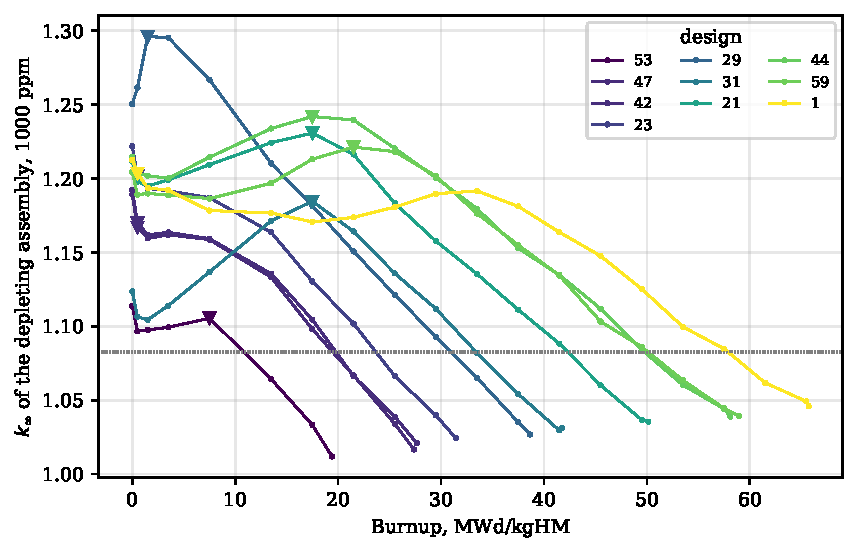
\includegraphics[width=0.95\linewidth]{images/swing_khist}
  \caption[Depletion histories of the Campaign 8 candidates]{Assembly infinite multiplication factor against burnup at \SI{1000}{ppm} for the eight front designs and the two two-bank representatives.}
  \label{fig:c8-swing-khist}
\end{figure}

\begin{table}[htbp]
  \centering
  \footnotesize
  \setlength{\tabcolsep}{3.0pt}
  \begin{threeparttable}
  \caption[Reactivity swing of the Campaign 8 candidates]{Gadolinium hump and burnup reactivity swing of the Campaign 8 candidates.}
  \label{tab:c8-swing}
  \begin{tabular}{@{}r r r r r r r r r r@{}}
    \toprule
    ID & $e$ & $k_\mathrm{BOL}$ & $k_\mathrm{peak}$ & $B_\mathrm{peak}$ & hump & $\Delta\rho_\mathrm{peak\to EOC}$ & $\Delta\rho_\mathrm{Xe\to EOC}$ & $c_\mathrm{BOL}$ & $c_\mathrm{peak}$ \\
    {[--]} & [wt\%] & [--] & [--] & [MWd/kgHM] & [pcm] & [pcm] & [pcm] & [ppm] & [ppm] \\
    \midrule
    53 & 3.45 & 1.1138 & 1.1055 & 7.5 & -676 & 1922 & 1196 & 1312 & 1312 \\
    47 & 4.39 & 1.1891 & 1.1670 & 0.5 & -1591 & 6673 & 6673 & 2348 & 2348 \\
    42 & 4.44 & 1.1922 & 1.1701 & 0.5 & -1578 & 6875 & 6875 & 2377 & 2377 \\
    23 & 4.94 & 1.2219 & 1.2019 & 0.5 & -1356 & 9184 & 9184 & 2979 & 2979 \\
    13 & 5.14 & 1.1302 & 1.1210 & -- & -723 & 3103 & 2106 & 1697 & 1697 \\
    29 & 5.90 & 1.2504 & 1.2961 & 1.5 & +2822 & 15225 & 13102 & 3677 & 4277 \\
    31 & 6.59 & 1.1236 & 1.1846 & 17.5 & +4580 & 7936 & 1971 & 1701 & 2760 \\
    21 & 7.81 & 1.2114 & 1.2307 & 17.5 & +1295 & 11136 & 8914 & 3752 & 4095 \\
    44 & 9.23 & 1.2147 & 1.2420 & 17.5 & +1812 & 11892 & 9340 & 4372 & 4940 \\
    59 & 9.34 & 1.2043 & 1.2212 & 21.5 & +1150 & 10538 & 8319 & 4112 & 4473 \\
    1 & 11.03 & 1.2127 & 1.2036 & 0.5 & -626 & 9257 & 9257 & 4674 & 4674 \\
    \bottomrule
  \end{tabular}
  \begin{tablenotes}\footnotesize
    \item Assembly $k_\infty$ at 1000\,ppm from the single-shot depletion of \nolinkurl{validate_ktarget_burnup.py} at the campaign fidelity. The hump is $\rho_\mathrm{peak} - \rho_\mathrm{BOL}$, xenon-free BOL. $\Delta\rho$ is measured to $\rho(k_\mathrm{target})$. The boron concentrations are linear extrapolations above 1000\,ppm with the 1000 to 1500\,ppm differential worth of the core. They are estimates: for design 47 the root of the measured reactivity curve is 2327\,ppm (Section~\ref{sec:res-c8-mtc}). $B_\mathrm{peak}$ was not recorded for design 13.
  \end{tablenotes}
  \end{threeparttable}
\end{table}

Four readings follow.

\begin{enumerate}
  \item Six of the eleven candidates have no hump. Designs 1, 13, 23,
        42, 47 and 53 reach their maximum at the first operating point,
        and their hump is negative, from $-626$ to \SI{-1591}{pcm}. For
        these designs the beginning-of-life state is the most reactive
        state of the cycle and the screens of
        Section~\ref{sec:meth-ctrl} screen the right state.

  \item The other five do have one, from $+1150$ to \SI{+4580}{pcm},
        with the maximum between \num{1.5} and
        \SI{21.5}{MWd/kgHM}. Design 31 carries the largest hump of the
        set and design 29 the largest of the front, at
        \SI{+2822}{pcm}.

  \item The hump is not ordered by the gadolinia loading of
        Table~\ref{tab:c8-front}. Design 1 carries \SI{7.43}{wt\%}
        gadolinia on forty pins and shows no hump, while design 29
        carries \SI{0.18}{wt\%} on forty pins and shows the largest
        hump of the front.

  \item The campaign was screened at a boron concentration well below
        the critical one. The extrapolated critical concentration at
        beginning of life runs from \num{1312} to \SI{4674}{ppm}, and
        at the operating maximum it reaches \SI{4940}{ppm} on design
        44. The values are linear extrapolations above \SI{1500}{ppm}
        and can err in either direction. For design 47 the root of the
        measured reactivity curve, \SI{2327}{ppm}, lies \SI{21}{ppm}
        below the linear value (Section~\ref{sec:res-c8-mtc}).
\end{enumerate}

The last reading is the one that bounds the interpretation of the whole
campaign. The screens were evaluated at the fixed \SI{1000}{ppm} of
Section~\ref{sec:meth-boron}, which is not the concentration at which
any of these cores would be critical at start-up. The direction of the
resulting bias is the one stated in
Section~\ref{sec:meth-boron-bias}, and the magnitudes here give it a
scale for the first time.

Two approximations bound the boron columns. The swing is an assembly
quantity while the differential boron worth is a core quantity measured
at beginning of life, so dividing one by the other assumes the worth
does not change over the cycle, which it does through the spectrum.
Both concentrations should be read to one significant figure.

%% AUTHOR: the physics of why six candidates show no hump while five
%% do, and whether the critical-boron column changes the reading of the
%% controllability result of Section~\ref{sec:res-c8-split}.

\subsection{Three-dimensional confirmation: the four closures}
\label{sec:res-c8-closures}

Four commitments were made earlier in this work and deferred to a
confirmation on the three-dimensional core model. This
subsection reports what each of them measured. Two are closed, one is
partly closed and one remains open.

The three-dimensional confirmation closes four commitments made earlier
in this work. Each is listed with the quantity that closes it, and
Table~\ref{tab:c8-closures} collects the measured closures.

\begin{enumerate}
  \item The second tier of the fidelity strategy of Section~\ref{sec:meth-fidelity}. Ten front designs were depleted in a single shot at the campaign fidelity with core solves at beginning and end of cycle. The leakage factor drifts by -152 to +149\,pcm between the two, within two standard deviations for 10 of 10 designs, and the implied cycle correction is -14 to +56\,EFPD.
  \item The axial correction of Section~\ref{sec:meth-lax}. On the three-dimensional core model the unrodded factor is 1.0286 to 1.0311, against the campaign value 1.0289 of the water-slab study, a gap of -25 to +211\,pcm. The two-bank factor is 1.0219 to 1.0252 and the four-bank factor 1.0126 to 1.0177.
  \item The three departures from the benchmark inputs stated in Section~\ref{sec:reactor-model}, tested on C8-21 and C8-47, which bracket the front. Raising the steel fraction of the heavy reflector from 0.90 to the benchmark 0.956 adds 199 and 182\,pcm to the unrodded three-dimensional core, so the adopted fraction is conservative. Narrowing the absorber radius from 0.4331\,cm to the benchmark boron carbide radius of 0.4229\,cm lowers the four-bank worth by 131 to 169\,pcm and the two-bank worth by 93 to 94\,pcm, about 1.5 per cent of the two-bank worth, against margins of 7000\,pcm and more. The coolant density is not exposed as a sensitivity and remains a stated departure.
  \item The rod-stack comparison. The two-dimensional screen with full-height boron carbide is conservative by 1272 to 2047\,pcm for four banks and 2062 to 2671\,pcm for two banks against the benchmark rod on the three-dimensional core. \openpoint{Closure 4: the full-B4C stack run that separates the stack from the leakage is pending.}
\end{enumerate}

\begin{table}[htbp]
  \centering
  \footnotesize
  \setlength{\tabcolsep}{4.0pt}
  \caption[Closures of the three-dimensional confirmation]{Measured closure of the four commitments carried by the three-dimensional confirmation.}
  \label{tab:c8-closures}
  \begin{tabularx}{\textwidth}{@{}>{\raggedright\arraybackslash}p{2.6cm} >{\raggedright\arraybackslash}X r >{\raggedright\arraybackslash}X r@{}}
    \toprule
    Closure & Quantity & Value & Quantity & Value \\
    \midrule
    1 Second tier & leakage-factor drift BOL to EOC [pcm] & -152 to +149 & implied cycle correction [EFPD] & -14 to +56 \\
    2 Axial correction & $L_\mathrm{ax,hw}$ unrodded & 1.0286 to 1.0311 & gap to the campaign 1.0289 [pcm] & -25 to +211 \\
    3a Reflector 0.956 & $\Delta\rho$ unrodded 3D [pcm] & +182 to +199 &  &  \\
    3b Absorber 0.4229 & $\Delta$ four-bank margin [pcm] & -169 to -131 & $\Delta$ two-bank margin [pcm] & -94 to -93 \\
    4 Rod stack & screen conservatism four-bank [pcm] & 1272 to 2047 & stack effect four-bank [pcm] & pending \\
    \bottomrule
  \end{tabularx}
\end{table}

Closure 1 is not an independent measurement. It is the same set of
solves reported in Section~\ref{sec:res-kt-burnup}, read there for the
burnup dependence of the leakage factor and read here as the second
fidelity tier. The drift range and the cycle correction of
Table~\ref{tab:c8-closures} are the drift and $\Delta\mathrm{EFPD}$
columns of Table~\ref{tab:kt-burnup}, and they are quoted once as
evidence for two different commitments.

Closures 2 and 4 are read in full in
Section~\ref{sec:res-c8-3d}, where the rodded axial factors, the
benchmark rod stack and the resulting conservatism of the
two-dimensional screen are measured design by design against
Table~\ref{tab:c8-post-3d1000}. The short statement is that the rodded
factors are smaller than the unrodded one, so the rodded
three-dimensional core is more subcritical than the two-dimensional
screen assumed, and the screen therefore rejected designs it did not
need to reject while admitting none that the three-dimensional core model would refuse.

The beginning-of-life margins above are reduced by the gadolinium hump of the operating maximum, -1723 to +4955\,pcm on the core. At the maximum the two-bank set at 1000\,ppm on the three-dimensional core excludes designs 1, 21, 23, 29, 31, 44, 59.

The hump range quoted here is the assembly hump of
Table~\ref{tab:c8-swing} carried to the core, which is larger than the
assembly value by the leakage factor, and it is applied to the
beginning-of-life margins because
Section~\ref{sec:res-kt-burnup} shows the leakage factor constant over
the cycle within the Monte Carlo noise.

%% AUTHOR: physics of the hump and its consequence for the candidate.

%% AUTHOR: whether the exclusion of seven of the ten candidates from
%% the two-bank set at the operating maximum is the argument that
%% decides the candidate list of Section~\ref{sec:res-c8-limits}, and
%% what the remaining designs have in common.

\subsection{Cycle length against the reported refuelling interval}
\label{sec:res-c8-mission}

The open record gives the prototype a refuelling interval of five
years~\cite{dinizcosta_2017}. The cycle
length that corresponds to it depends on the capacity factor, which
no open source states.

\begin{equation}
\mathrm{EFPD}_\mathrm{req} = 365.25\, T_\mathrm{cal}\, \mathrm{CF}
\label{eq:mission-efpd}
\end{equation}

\noindent where the symbols have the following meaning.

\begin{itemize}
  \item $\mathrm{EFPD}_\mathrm{req}$ is the cycle length that meets the
        refuelling interval, in effective full power days.

  \item $T_\mathrm{cal}$ is the calendar interval, in years, equal to
        five.

  \item $\mathrm{CF}$ is the capacity factor, dimensionless, assumed
        between 0.5 and 0.8 for a naval prototype and stated as an
        assumption.
\end{itemize}

Five years at a capacity factor of 0.8 is 1461 EFPD, and at 0.5 it is
913 EFPD. Every design on the front exceeds the former, the shortest by
a third and the longest by a factor of four, and design 53 in the
two-bank subset meets it at 1142 EFPD with ring enrichments of 2.5,
3.1 and \SI{4.0}{wt\%}. The reported enrichment figures locate on the
same axis. The 6 to \SI{8}{wt\%} stated in 2014 corresponds to designs
31 and 21, at 3381 and 4221 EFPD, and the \SI{19}{wt\%} reported in
2025 lies above the search box and, on the evidence of the axial study,
above what the regulating banks of this core can hold. The comparison
is conservative on two counts. Every cycle length is a lower bound
for a core operated with boron letdown
(Section~\ref{sec:res-c8-post-limits}), and the burnup dependence of
the leakage factor corrects the six longest cycles downward
(Section~\ref{sec:res-kt-burnup}).

The consequence for the design problem is stated as a finding. The
objective of maximising cycle length pushes every design far beyond
the reported requirement and, in doing so, onto the control boundary.
Cycle length is not the binding requirement of this core. The binding
requirements are controllability and peaking, and the cycle length
belongs among the constraints, at the required value. Campaign 9 poses
the problem that way (Section~\ref{sec:res-c9}).

\subsection{The pre-registered expectations, scored}
\label{sec:res-c8-hyp}

Table~\ref{tab:c8-hyp-scored} scores the eight expectations written before
the design of experiments closed against the measurement.

\begin{table}[htbp]
  \centering
  \small
  \caption{The eight expectations written before the design of
  experiments closed, against the measurement.}
  \label{tab:c8-hyp-scored}
  \begin{tabularx}{\textwidth}{@{}>{\raggedright\arraybackslash}X>{\raggedright\arraybackslash}p{1.6cm}>{\raggedright\arraybackslash}X@{}}
    \toprule
    Expectation & Outcome & Measurement \\
    \midrule
    Peaking floor rises to about 1.60 & Failed & Floor 1.510, reached through low enrichment rather than a thick reflector \\
    Cycles 450 to 500 EFPD shorter than uncorrected & Not testable & No uncorrected Campaign 8 run exists, and the box differs from Campaign 7 \\
    Two banks worth half of sixteen & Held & Ratio 0.473 to 0.511, mean 0.496, on all 60 designs \\
    Two-bank window below about 1.074 & Held & Feasible two-bank designs at 1.026 to 1.042, median implied ceiling 1.069 \\
    Ceiling binds rarely and after the screen & Held & Zero designs rejected by the ceiling alone \\
    Every block moves all four variables & Partly held & Block 1 held $w_\mathrm{Gd}$ fixed, every block moved three or more and returned feasible designs \\
    Design-of-experiments feasibility below \SI{31}{\%} & Held & 9 of 36, \SI{25}{\%} \\
    No censoring, no design near \SI{75}{MWd/kgHM} & Held on the front & No censoring. One infeasible design at \SI{79.6}{MWd/kgHM}, the front maximum is 57.7 \\
    \bottomrule
  \end{tabularx}
\end{table}

\subsection{Cost}
\label{sec:res-c8-cost}

The campaign cost \SI{75684}{s}, \SI{1261}{s} per evaluation, against
\SI{949}{s} in Campaign 7 on the AWS instance. The archive now records
every transport phase separately, so the breakdown is measured rather
than apportioned: assembly solve \SI{11}{s}, core solve \SI{107}{s},
depletion \SI{925}{s}, and the two rodded solves \num{100} and
\SI{102}{s}. Those five phases sum to \SI{1245}{s}, so the residual
\SI{16}{s} per evaluation, \SI{1.3}{\%}, is the non-transport
overhead of the evaluation call. The two rodded solves are
\SI{16.0}{\%} of the evaluation and \SI{16.2}{\%} of its transport. The depletion dominates because the cycles are long, 14.6
transport states per design against 13.0 in Campaign 7. The measured
particle rate on the 64 threads of wks720, \num{5734} per second,
equals that of the 32 cores of the AWS instance, so the difference in
wall time is the third core solve and the longer depletions, not the
machine.

\subsection{Limitations and the candidate list}
\label{sec:res-c8-limits}

Five limitations bound the claims of this section.

\begin{enumerate}
  \item Five designs, 15, 24, 26, 28 and 48, reached the active
        batches with the fission-source entropy not yet converged. None
        is on the front or in the two-bank subset.

  \item The statistical error on $F_{\Delta H}$ remains unmeasured.
        Adjacent front designs differ by 0.008 to 0.051 in peaking, and
        the ordering of the three lowest, 47, 42 and 23, is not
        resolved until the core tally errors are read.

  \item Designs 54 and 11 fail the control screen by 17 and
        \SI{63}{pcm}, within the resolution of one core solve at
        \num{100000} particles. They are marginal, not rejected, and
        are re-scored with seed replicates before the candidate list is
        final.

  \item The control screen is evaluated at the benchmark boron
        concentration and at the model's fixed temperatures. It tests
        whether the regulating banks hold the fresh core subcritical at
        power with \SI{1000}{ppm} present. It is not a shutdown-margin
        demonstration, which requires the cold state, all banks minus
        the highest-worth assembly, and the boron worth stated
        explicitly. The boron worth of the candidates is measured in
        the confirmation study of Section~\ref{sec:meth-boron-worth}.

  \item The convergence claim is one block short of the formal rule of
        Section~\ref{sec:meth-loop}, which requires the hypervolume
        gain to stay below one per cent for three consecutive
        iterations. Campaign 8 ran four infill blocks and the gain fell
        below the threshold in the last two, so the third consecutive
        observation is missing. The front is reported as the best
        available rather than as a converged one.
\end{enumerate}

Two candidate lists follow from the campaign, and they are different
answers to different questions.

\begin{enumerate}
  \item For the longest cycle at a stated peaking, the front of
        Table~\ref{tab:c8-front}, with designs 47, 23 and 21 as the
        representatives of its three regions: the short-cycle floor,
        the knee, and the long-cycle boundary.

  \item For a core that operates like a pressurised water reactor,
        with the regulating banks withdrawn at power and the reported
        refuelling interval met, the two-bank subset of
        Table~\ref{tab:c8-two}, with design 53 as the representative
        that meets five years at a capacity factor of 0.8 and design 31
        as the representative at the enrichment reported in 2014.
\end{enumerate}

The three-dimensional confirmation of
Section~\ref{sec:res-c8-closures}, with the axial structures of the assembly, the core barrel and the boron worth, decides between them.

The candidate of the Campaign 8 formulation is design 47, for the
reasons set out in Section~\ref{sec:res-c8-decision} after the
post-analysis has been reported. Campaign 9 then searches the same
design space under the reformulated problem (Section~\ref{sec:res-c9}).


% ---------------------------------------------------------------------
%  Post-analysis of the Campaign 8 candidates.
%  Figures images/c8_post_*.pdf and tables tab:c8-post-* generated by
%  c8_post_figures.py from out_c8, boron_c8, confirm3d_c8_0ppm,
%  confirm3d_c8_dc37, confirm3d_c8_noparked and boron_c8_marginal.
% ---------------------------------------------------------------------

\section{Post-analysis of the Campaign 8 candidates}
\label{sec:res-c8-post}

The archive of Campaign 8 fixes the front at 1000\,ppm of soluble boron
and at beginning of life. The post-analysis asks what the front looks
like under other readings of the same designs. Six studies were run on
eleven designs, the eight members of the feasible front and the three
feasible designs that satisfy the two-bank reading of
Section~\ref{sec:meth-ctrl}.

\begin{enumerate}
  \item A boron sweep at 0, 500, 1000 and 1500\,ppm in three rod
        states, all rods out, the four regulating banks inserted, and the
        first two regulating banks inserted, on the two-dimensional core
        with one seed (132 solves).

  \item A zero-boron hold-down check under the four regulating banks on
        the two-dimensional core and on the three-dimensional core model with the axial structures of the assemblies, barrel and vessel, two seeds (44 solves).

  \item A three-dimensional confirmation at 1000\,ppm in the three rod
        states, two seeds, for all eleven designs.

  \item A parked-rod sensitivity on design 47 with all rods out.

  \item A re-score with three seeds of the two designs that fail the
        control screen by less than the solve resolution.

  \item A downcomer sensitivity on three thick-reflector designs, with
        the reflector thinned to 3.969\,cm so that the downcomer is 3.7\,cm.
\end{enumerate}

Two rodded states are used throughout this section. The first is
$k_\mathrm{RE}$, with the four regulating banks RE1 to RE4 inserted in
the sixteen inner assemblies. The second is $k_\mathrm{RE12}$, with RE1
and RE2 inserted in eight assemblies. The sixteen outer SH assemblies
are reserved for shutdown and are never inserted in any screen. The
figures of this section carry the code label ALL-RE for the state
written $k_\mathrm{RE}$ here, for the reason given in
Section~\ref{sec:meth-ctrl}.
Figure~\ref{fig:c8-post-banks} shows the map. The same bank assignment
is used by every screen of Campaign 8, and the enrichment rings coincide
with the banks: ring C with RE1, ring M with RE2 to RE4 and ring P with
SH.

\begin{figure}[htbp]
  \centering
  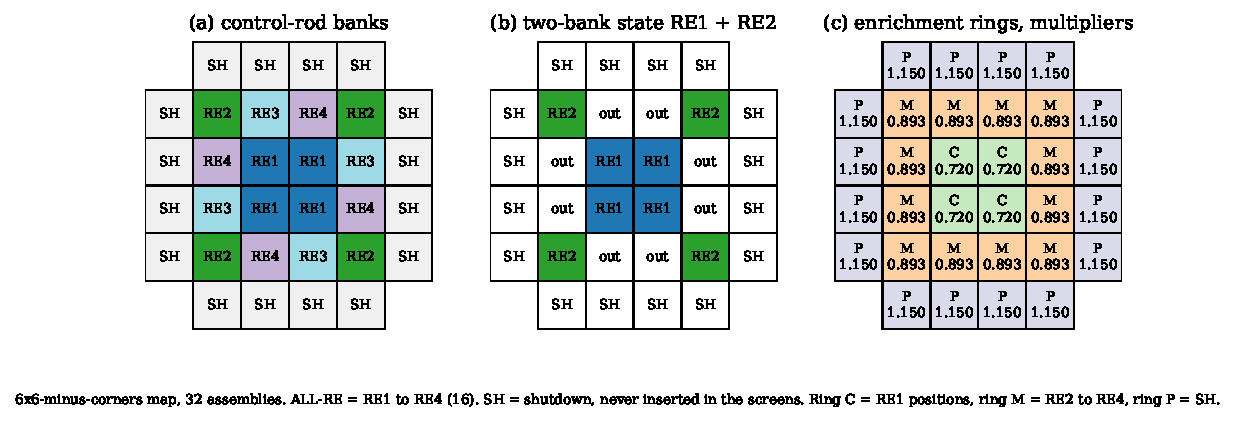
\includegraphics[width=\textwidth]{images/c8_post_core_banks_rings}
  \caption[The 32-assembly map of Campaign 8]{The 32-assembly map of Campaign 8. (a)~The four regulating banks and the shutdown bank. (b)~The two-bank state RE1 + RE2. (c)~The three enrichment rings with their multipliers.}
  \label{fig:c8-post-banks}
\end{figure}

All reactivities are quoted in pcm through the usual definition.

\begin{equation}
\rho = 10^{5}\,\frac{k - 1}{k}
\label{eq:rho-pcm}
\end{equation}

\noindent where the symbols have the following meaning.

\begin{itemize}
  \item $\rho$ is the reactivity, in pcm.
  \item $k$ is the effective multiplication factor of the core in the
        state considered, dimensionless.
\end{itemize}

The controllability screen is the one defined in
Equation~\eqref{eq:g-ctrl-meth} of Section~\ref{sec:meth-ctrl}, applied
by the evaluator on the eigenvalue itself and not on the reactivity. It
reads $k_\mathrm{RE} \leq 0.99$, that is a required margin
$\Delta k_\mathrm{margin} = 0.01$, which is \SI{1010}{pcm} on the
reactivity axis of this section.

The margin is a design reserve rather than a cited limit. It covers the
Monte Carlo uncertainty of the solve itself, which is 20 to 28\,pcm per
solve in the post-analysis, the temperature and xenon states that a
beginning-of-life eigenvalue at hot full power does not span, and the
reactivity that an operator holds in hand rather than at the point of
criticality.

Equation~\eqref{eq:g-ctrl-meth} expresses the margin in $\Delta k$, whereas
the margins reported below are reactivities, so the threshold on those
figures is $-\rho(0.99) = 1010$\,pcm rather than 1000\,pcm. No design
of the archive or of the post-analysis falls inside that 10\,pcm band,
so the two conventions separate the same designs.

\subsection{Two controllability tiers}
\label{sec:res-c8-tiers}

Feasibility in Campaign 8 is set by the four-bank screen alone. The
two-bank reading $g_\mathrm{ctrl12}$ is recorded for every design and
never constrained, so the archive can be split after the fact. Of the
19 feasible designs, four satisfy $k_\mathrm{RE12} \leq 0.99$ at
1000\,ppm, namely 12, 13, 31 and 53. None of them lies on the feasible
front. Their own front, after removing design 12, which is dominated by
53, has three members.
Table~\ref{tab:c8-post-tiers} lists both tiers and
Figure~\ref{fig:c8-post-front} places them in the objective plane.
Tier A is the feasible front and tier B the front of the designs that also
satisfy $k_\mathrm{RE12} \leq 0.99$. In the table $W_{16}$ and $W_8$ are
the beginning-of-life worths of the four regulating banks and of
RE1 + RE2. In the figure blue circles are feasible designs that need the
four regulating banks at 1000\,ppm, green squares are feasible designs
controllable with RE1 + RE2, and the two lines are the two fronts. The
error bars are one seed-to-seed standard deviation of $F_{\Delta H}$ at
the archive fidelity, about 0.011, and the dotted lines mark four and
five calendar years at 48\,MWth for an assumed capacity factor of 0.8.

\begin{table}[htbp]
  \centering
  \footnotesize
  \caption{Campaign 8 candidates in two controllability tiers, archive values at 1000\,ppm.}
  \label{tab:c8-post-tiers}
  \setlength{\tabcolsep}{3pt}\scriptsize
  \begin{tabular}{@{}c l r r r r r r r r r r r@{}}
    \toprule
    Tier & ID & $e$ & $e_\mathrm{max}$ & Gd & pins & $t_\mathrm{refl}$ & EFPD & $B_\mathrm{EOC}$ & $F_{\Delta H}$ & $k_\mathrm{core}$ & $W_{16}$ & $W_8$ \\
         &    & wt\% & wt\% & wt\% &  & cm &  & MWd/kg &  &  & pcm & pcm \\
    \midrule
    A & 47 & 4.39 & 5.05 & 2.88 & 12 & 4.29 & 1941 & 19.4 & 1.510 & 1.0981 & 17058 & 7881 \\
    A & 42 & 4.44 & 5.11 & 2.88 & 12 & 3.76 & 1968 & 19.6 & 1.522 & 1.1008 & 17035 & 7810 \\
    A & 23 & 4.94 & 5.68 & 2.80 & 12 & 4.81 & 2346 & 23.4 & 1.534 & 1.1316 & 16348 & 7596 \\
    A & 29 & 5.90 & 6.79 & 0.18 & 40 & 4.69 & 3070 & 30.6 & 1.542 & 1.1578 & 15223 & 6997 \\
    A & 21 & 7.81 & 8.99 & 3.11 & 32 & 4.92 & 4221 & 42.1 & 1.592 & 1.1264 & 14096 & 6405 \\
    A & 44 & 9.23 & 10.61 & 3.20 & 40 & 5.33 & 5019 & 50.1 & 1.612 & 1.1316 & 13178 & 5950 \\
    A & 59 & 9.34 & 10.75 & 4.32 & 40 & 5.66 & 5104 & 51.0 & 1.634 & 1.1198 & 13201 & 6014 \\
    A & 1 & 11.03 & 12.68 & 7.43 & 40 & 3.94 & 5782 & 57.7 & 1.677 & 1.1306 & 12775 & 5830 \\
    \midrule
    B & 53 & 3.45 & 3.97 & 2.92 & 12 & 4.74 & 1142 & 11.4 & 1.524 & 1.0263 & 18401 & 8384 \\
    B & 13 & 5.14 & 5.91 & 5.25 & 24 & 3.15 & 2383 & 23.8 & 1.632 & 1.0424 & 16957 & 7684 \\
    B & 31 & 6.59 & 7.58 & 3.38 & 40 & 4.18 & 3381 & 33.8 & 1.650 & 1.0339 & 15030 & 6791 \\
    \bottomrule
  \end{tabular}
\end{table}

\begin{figure}[htbp]
  \centering
  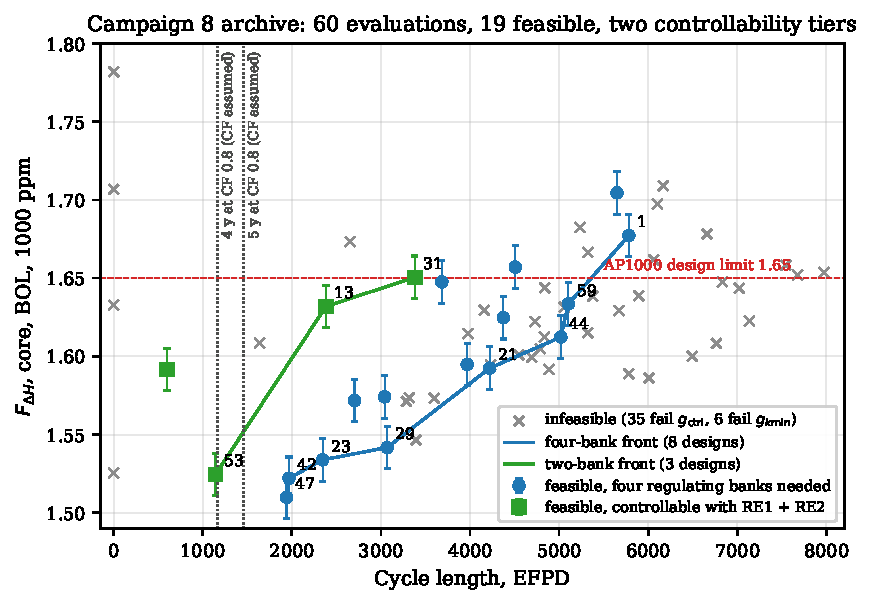
\includegraphics[width=0.9\textwidth]{images/c8_post_front_two_tier}
  \caption{The Campaign 8 archive in the objective plane, by controllability tier.}
  \label{fig:c8-post-front}
\end{figure}

Tier A is the feasible front, 47, 42, 23, 29, 21, 44, 59 and 1, from
1941 to 5782\,EFPD and $F_{\Delta H}$ from 1.510 to 1.677. Tier B is the
two-bank front, 53, 13 and 31, from 1142 to 3381\,EFPD and
$F_{\Delta H}$ from 1.524 to 1.650. At equal peaking the two-bank
requirement costs between 34 and 51\,\% of the cycle length. At
$F_{\Delta H} \approx 1.52$, tier A gives 1941 to 1968\,EFPD and tier B
gives 1142\,EFPD. At $F_{\Delta H} \approx 1.64$, tier A gives
5104\,EFPD and tier B gives 3381\,EFPD.

The two tiers are defined by the two-dimensional screen of the
campaign. The three-dimensional confirmation of
Section~\ref{sec:res-c8-3d} moves the boundary. At 1000\,ppm the
RE1 + RE2 margin of design 47 is $-1091$\,pcm on the two-dimensional
core and $+1330$\,pcm on the three-dimensional core model, and that of design 42 goes from $-1315$ to $+1052$\,pcm.
Table~\ref{tab:c8-post-3d1000} and Figure~\ref{fig:c8-post-margins1000}
show the eleven confirmed designs. In the table
$L_\mathrm{ax} = k_\mathrm{2D}/k_\mathrm{3D}$ for each rod state, the
margins are $-\rho$ of the rodded core, positive when subcritical,
$F_{\Delta H}^\mathrm{3D}$ is axially integrated, and the two-bank column
applies the screen $k_\mathrm{RE12} \leq 0.99$, that is 1010\,pcm. In the
figure dark bars are the two-dimensional core of the campaign screen and
light bars the three-dimensional core model with barrel and vessel wall, blue is the four-bank state and green the two-bank state, and the
dashed line is the screen of Equation~\eqref{eq:g-ctrl-meth}. Under the
three-dimensional reading
the two-bank set at 1000\,ppm and beginning of life is 53, 13, 31, 47
and 42, and design 23 stays out at $-1718$\,pcm. That
set is not the same as the set at the operating maximum of
Section~\ref{sec:res-c8-closures}, which is 53, 47 and 42, because the
gadolinium hump of design 31 removes \SI{4955}{pcm} of its
beginning-of-life two-bank margin of \SI{5856}{pcm} and leaves it below
the screen. Measured against
Equation~\eqref{eq:g-ctrl-meth} in its own units, design 42 satisfies the
two-bank screen by 41\,pcm, which is less than two seed standard
deviations of a single solve, so its two-bank status is not resolved by
this pair of solves. Design 47 satisfies it by 313\,pcm and is
resolved. The cost of two-bank control quoted above is
therefore a statement about the two-dimensional screen. On the
three-dimensional core it vanishes at the low-peaking floor, where
design 47 itself is two-bank controllable, and it remains 34\,\% at
$F_{\Delta H} \approx 1.64$, where design 31 stands against design 59.

\begin{table}[htbp]
  \centering
  \footnotesize
  \caption{Three-dimensional confirmation at 1000\,ppm, two seeds per solve, $150\,000 \times 200$.}
  \label{tab:c8-post-3d1000}
  \setlength{\tabcolsep}{3pt}\scriptsize
  \begin{tabular}{@{}l r r r r r r r r r r r@{}}
    \toprule
    ID & $e$ & $L_\mathrm{ax}^\mathrm{ARO}$ & $L_\mathrm{ax}^\mathrm{RE}$ & $L_\mathrm{ax}^\mathrm{RE12}$ & $M_{16}^\mathrm{2D}$ & $M_{16}^\mathrm{3D}$ & $M_8^\mathrm{2D}$ & $M_8^\mathrm{3D}$ & $F_{\Delta H}^\mathrm{2D}$ & $F_{\Delta H}^\mathrm{3D}$ & two-bank in 3D \\
       & wt\% &  &  &  & pcm & pcm & pcm & pcm &  &  &  \\
    \midrule
    53 & 3.45 & 1.0311 & 1.0177 & 1.0252 & 15857 & 17904 & 5882 & 8553 & 1.494 & 1.475 & yes \\
    47 & 4.39 & 1.0304 & 1.0163 & 1.0245 & 8123 & 9891 & -1091 & 1330 & 1.531 & 1.503 & yes \\
    42 & 4.44 & 1.0302 & 1.0162 & 1.0240 & 7894 & 9638 & -1315 & 1052 & 1.532 & 1.515 & yes \\
    23 & 4.94 & 1.0307 & 1.0161 & 1.0243 & 4759 & 6443 & -4046 & -1718 & 1.525 & 1.522 & no \\
    13 & 5.14 & 1.0301 & 1.0137 & 1.0230 & 12842 & 14388 & 3562 & 5946 & 1.603 & 1.573 & yes \\
    29 & 5.90 & 1.0303 & 1.0151 & 1.0236 & 1598 & 3136 & -6615 & -4412 & 1.527 & 1.491 & no \\
    31 & 6.59 & 1.0288 & 1.0146 & 1.0228 & 11768 & 13399 & 3491 & 5856 & 1.627 & 1.596 & yes \\
    21 & 7.81 & 1.0291 & 1.0146 & 1.0229 & 2803 & 4307 & -4776 & -2598 & 1.585 & 1.576 & no \\
    44 & 9.23 & 1.0288 & 1.0145 & 1.0226 & 1519 & 2990 & -5637 & -3508 & 1.630 & 1.600 & no \\
    59 & 9.34 & 1.0288 & 1.0145 & 1.0232 & 2502 & 3989 & -4691 & -2479 & 1.625 & 1.603 & no \\
    1 & 11.03 & 1.0286 & 1.0126 & 1.0219 & 1198 & 2470 & -5761 & -3700 & 1.673 & 1.642 & no \\
    \bottomrule
  \end{tabular}
\end{table}

\begin{figure}[htbp]
  \centering
  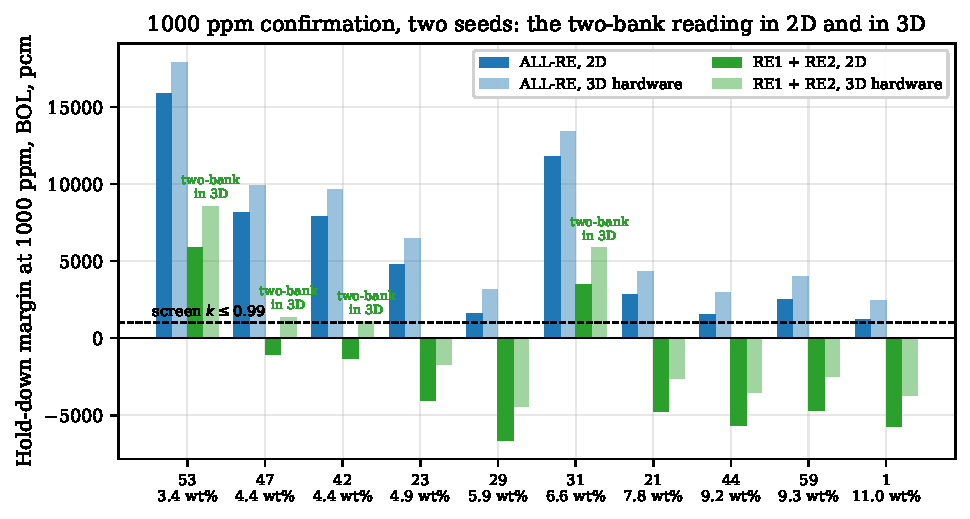
\includegraphics[width=\textwidth]{images/c8_post_margins_1000_2d3d}
  \caption{Hold-down margins at 1000\,ppm and beginning of life for the eleven confirmed designs, two seeds per solve.}
  \label{fig:c8-post-margins1000}
\end{figure}

Designs 47 and 42 are twins. They differ by 0.05\,wt\% in enrichment,
by 0.003\,wt\% in gadolinia and by 0.53\,cm in reflector thickness, and
they sit 27\,EFPD and 0.012 in $F_{\Delta H}$ apart, both within the
solve noise of Section~\ref{sec:res-c8-sigma}. The acquisition function
accepted both because the reflector thickness alone satisfied the
minimum separation of 0.14 in the normalised design space, and the
reflector is nearly inert in this box, as Section~\ref{sec:res-c8-refl}
shows. This is a limitation of separation measured in design space
rather than in objective space.

\subsection{Boron sweep}
\label{sec:res-c8-boron}

The sweep measures four quantities per design and per concentration.

\begin{equation}
M_n(c) = -\rho\!\left(k_n(c)\right)
\label{eq:margin}
\end{equation}

\noindent where the symbols have the following meaning.

\begin{itemize}
  \item $M_n(c)$ is the hold-down margin with $n$ rodded assemblies at
        boron concentration $c$, in pcm. It is positive when the rodded
        core is subcritical.
  \item $k_n(c)$ is the eigenvalue of the core with the $n$ assemblies
        rodded, dimensionless. $n = 16$ is the RE state and $n = 8$ is
        RE12.
  \item $c$ is the soluble boron concentration, in ppm.
\end{itemize}

\begin{equation}
W_n(c) = \rho\!\left(k_\mathrm{ARO}(c)\right) - \rho\!\left(k_n(c)\right)
\label{eq:bank-worth-rho}
\end{equation}

\noindent where the symbols have the following meaning.

\begin{itemize}
  \item $W_n(c)$ is the worth of the $n$ rodded assemblies at
        concentration $c$, in pcm.
  \item $k_\mathrm{ARO}(c)$ is the eigenvalue with all rods out,
        dimensionless.
\end{itemize}

Equation~\eqref{eq:bank-worth-rho} is the reactivity form of
Equation~\eqref{eq:bank-worth}, which states the same worth in units of
$k$, and it generalises it to any bank set.

The boron worth $W_B$ and the boron share $s_B$ are the quantities of
Equations~\eqref{eq:boron-worth} and~\eqref{eq:boron-share} of
Section~\ref{sec:meth-boron}, evaluated between 0 and \SI{1000}{ppm}.
The margin of Equation~\eqref{eq:margin} generalises
Equation~\eqref{eq:rod-only-margin} to a bank set of $n$ assemblies.

Table~\ref{tab:c8-post-boron} gives the results and
Figure~\ref{fig:c8-post-margin} shows the margins against
concentration. In the table $W_B$ is the differential boron worth between
0 and 1000\,ppm, and $M_{16}$ and $M_8$ are the hold-down margins under
the four regulating banks and under RE1 + RE2, positive when
subcritical. $c_8$ and $c_{16}$ are the boron concentrations at which the
two margins reach the screen value $k \leq 0.99$, that is 1010\,pcm, by
linear interpolation between the sweep points, and entries marked e are
extrapolated beyond 1500\,ppm. In the figure the left panel holds the
four regulating banks and the right panel RE1 + RE2, solid lines are
front members, dashed lines are the retained two-bank designs, and the
dashed horizontal line is the screen of Equation~\eqref{eq:g-ctrl-meth}.
Three regularities stand out.

\begin{table}[htbp]
  \centering
  \footnotesize
  \caption{Boron sweep of the eleven designs, two-dimensional core, one seed, $150\,000$ particles and 200 batches.}
  \label{tab:c8-post-boron}
  \setlength{\tabcolsep}{2.5pt}\scriptsize
  \begin{tabular}{@{}l l r r r r r r r r r@{}}
    \toprule
    ID & set & $W_B$ & $M_{16}(0)$ & $M_{16}(1000)$ & $M_8(1000)$ & $M_8(1500)$ & $c_{16}$ & $c_8$ & $W_8/W_{16}$ & share \\
       &     & pcm/ppm & pcm & pcm & pcm & pcm & ppm & ppm &  &  \\
    \midrule
    53 & two-bank & 8.54 & 7537 & 15881 & 5867 & 9958 & 0 & 415 & 0.457 & 0.317 \\
    47 & front & 6.98 & 1382 & 8144 & -1053 & 2212 & 0 & 1316 & 0.461 & 0.290 \\
    42 & front & 6.88 & 1225 & 7946 & -1287 & 1977 & 0 & 1352 & 0.460 & 0.287 \\
    23 & front & 6.31 & -1308 & 4745 & -4068 & -1119 & 380 & 1861e & 0.461 & 0.278 \\
    13 & two-bank & 6.14 & 7022 & 12937 & 3581 & 6420 & 0 & 566 & 0.448 & 0.266 \\
    29 & front & 5.22 & -3452 & 1574 & -6643 & -4156 & 886 & 2539e & 0.459 & 0.256 \\
    31 & two-bank & 4.79 & 7221 & 11832 & 3455 & 5763 & 0 & 472 & 0.446 & 0.241 \\
    21 & front & 4.18 & -1180 & 2877 & -4783 & -2851 & 533 & 2499e & 0.455 & 0.229 \\
    44 & front & 3.50 & -1816 & 1523 & -5678 & -3914 & 846 & 2895e & 0.453 & 0.210 \\
    59 & front & 3.54 & -835 & 2477 & -4677 & -3013 & 551 & 2709e & 0.456 & 0.212 \\
    1 & front & 3.13 & -1682 & 1228 & -5764 & -4293 & 926 & 3302e & 0.453 & 0.197 \\
    \bottomrule
  \end{tabular}
\end{table}

\begin{enumerate}
  \item The two-bank worth is a fixed fraction of the four-bank worth.
        Over the eleven designs $W_8 / W_{16}$ lies between 0.446 and
        0.461, and over all 60 archive designs it is $0.458 \pm 0.007$.
        The fraction does not depend on enrichment, gadolinia loading or
        reflector thickness. It is a property of the map of
        Figure~\ref{fig:c8-post-banks}, in which RE1 and RE2 occupy the
        eight positions of highest importance.

  \item Both the bank worth and the boron worth fall with enrichment.
        $W_{16}$ at 1000\,ppm decreases from 18\,401\,pcm at 3.45\,wt\% to
        12\,775\,pcm at 11.0\,wt\%, with a correlation of $-0.95$ with
        enrichment across the archive. The differential boron worth
        decreases from 8.54 to 3.13\,pcm/ppm over the same range. Both
        follow the hardening of the spectrum.

  \item Boron carries a minority of the hold-down capacity. The share
        $s_B$ lies between 0.197 and 0.317. At 1000\,ppm the four
        regulating banks carry between 68 and 80\,\% of the beginning-of-life
        hold-down of every candidate.
\end{enumerate}

\begin{figure}[htbp]
  \centering
  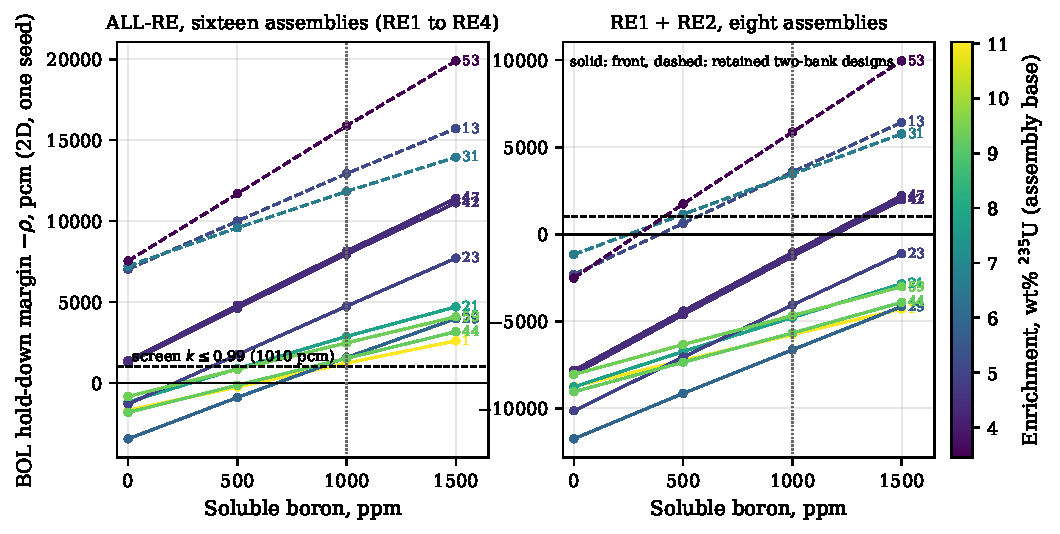
\includegraphics[width=\textwidth]{images/c8_post_margin_vs_boron}
  \caption{Beginning-of-life hold-down margin against soluble boron for the eleven designs, two-dimensional core, one seed.}
  \label{fig:c8-post-margin}
\end{figure}

The first regularity makes the two-bank margin predictable from the
four-bank one.

\begin{equation}
M_8(c) \approx M_{16}(c) - \left(1 - r\right) W_{16}(c)
\label{eq:m8-from-m16}
\end{equation}

\noindent where the symbols have the following meaning.

\begin{itemize}
  \item $M_8(c)$ and $M_{16}(c)$ are the margins of
        Equation~\eqref{eq:margin}, in pcm.
  \item $W_{16}(c)$ is the four-bank worth of
        Equation~\eqref{eq:bank-worth-rho}, in pcm.
  \item $r$ is the ratio $W_8 / W_{16}$, equal to 0.458 for this map,
        dimensionless.
\end{itemize}

Read through the boron concentration, the sweep gives the concentration
at which each design reaches the screen of Equation~\eqref{eq:g-ctrl-meth}
with eight rods, by linear interpolation between the sweep points.
Figure~\ref{fig:c8-post-boron} shows it, with the values that lie beyond
the 1500\,ppm sweep point marked as extrapolated. The three tier B designs reach
it at 415, 472 and 566\,ppm. The twins 47 and 42 reach it at 1316 and
1352\,ppm, about 35\,\% above the screen value. The remaining front
members need 1861 to 3302\,ppm, the last four by extrapolation beyond
the sweep. The screen at 1000\,ppm is therefore a modelling choice that
separates the front from two-bank control by a margin that the twins
could close with a higher beginning-of-cycle concentration, whereas the
long-cycle designs could not within any concentration used at power.
%% AUTHOR: state here the beginning-of-cycle boron concentrations of the
%% reference designs already cited in sec:meth-boron-basis, so that the
%% 1300 to 1350 ppm of the twins is placed against a cited range rather
%% than against a general statement.

\begin{figure}[htbp]
  \centering
  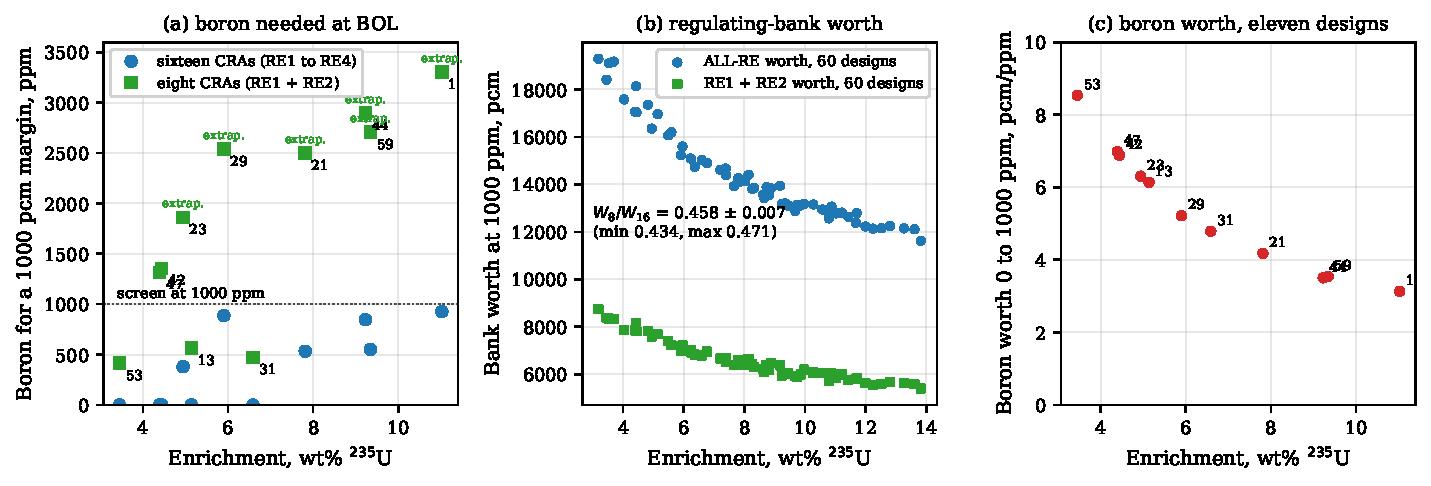
\includegraphics[width=\textwidth]{images/c8_post_boron_required_and_worths}
  \caption[Soluble boron and bank worths of the Campaign 8 designs]{Soluble boron and bank worths. (a)~Soluble boron needed at beginning of life for the screen margin with sixteen and with eight rodded assemblies, eleven designs. (b)~Four-bank and two-bank worth at 1000\,ppm, 60 archive designs. (c)~Differential boron worth, eleven designs.}
  \label{fig:c8-post-boron}
\end{figure}

The sweep closes on the archive. At 1000\,ppm the sweep eigenvalues
differ from the archive values by $-72$ to $+50$\,pcm over the 33
comparisons, with the archive solves at $100\,000 \times 170$ particles
and batches and the sweep at $150\,000 \times 200$.

\subsection{Zero-boron hold-down by the regulating banks}
\label{sec:res-c8-zeroboron}

Stage D asks whether the four regulating banks alone hold the
beginning-of-life core subcritical with no soluble boron, on the
two-dimensional core and on the three-dimensional core with the
benchmark rod stack. Table~\ref{tab:c8-post-zeroboron} and
Figure~\ref{fig:c8-post-zero} give the result. In the table
$L_\mathrm{ax}$ is $k_\mathrm{2D}/k_\mathrm{3D}$ for the rodded state with
the benchmark rod stack: bottom 12.04\,cm unrodded, 30.48\,cm Ag-In-Cd and
77.48\,cm B$_4$C. In the figure grey is the one-seed sweep, blue the
two-seed two-dimensional solve of stage D and orange the three-dimensional core model with the axial structures of the assemblies, barrel and vessel wall. Green markers meet the screen $k \leq 0.99$, orange markers are
subcritical below it and red markers are supercritical. The condition
tested is
the following.

\begin{table}[htbp]
  \centering
  \footnotesize
  \caption{Zero-boron hold-down by the four regulating banks alone at beginning of life, stage D, two seeds per solve.}
  \label{tab:c8-post-zeroboron}
  \begin{tabular}{@{}l r r r r r r l@{}}
    \toprule
    ID & $e$ & $k_\mathrm{2D}$ & $k_\mathrm{3D}$ & $M_{16}^\mathrm{2D}$ & $M_{16}^\mathrm{3D}$ & $L_\mathrm{ax}$ & reading \\
       & wt\% &  &  & pcm & pcm &  &  \\
    \midrule
    53 & 3.45 & 0.9301 & 0.9134 & 7518 & 9486 & 1.0183 & holds with margin \\
    47 & 4.39 & 0.9860 & 0.9702 & 1419 & 3069 & 1.0163 & holds with margin \\
    42 & 4.44 & 0.9872 & 0.9724 & 1301 & 2841 & 1.0152 & holds with margin \\
    23 & 4.94 & 1.0130 & 0.9966 & -1281 & 341 & 1.0164 & subcritical, margin < 1000 \\
    13 & 5.14 & 0.9346 & 0.9220 & 6996 & 8454 & 1.0136 & holds with margin \\
    29 & 5.90 & 1.0356 & 1.0201 & -3440 & -1967 & 1.0153 & supercritical \\
    31 & 6.59 & 0.9325 & 0.9201 & 7237 & 8684 & 1.0135 & holds with margin \\
    21 & 7.81 & 1.0110 & 0.9968 & -1089 & 318 & 1.0142 & subcritical, margin < 1000 \\
    44 & 9.23 & 1.0187 & 1.0048 & -1839 & -476 & 1.0139 & supercritical \\
    59 & 9.34 & 1.0086 & 0.9942 & -853 & 581 & 1.0145 & subcritical, margin < 1000 \\
    1 & 11.03 & 1.0173 & 1.0049 & -1699 & -491 & 1.0123 & supercritical \\
    \bottomrule
  \end{tabular}
\end{table}

\begin{equation}
k_\mathrm{RE}^\mathrm{3D}(0) \leq 1 - \Delta k_\mathrm{margin} = 0.99
\label{eq:boronfree-necessary}
\end{equation}

\noindent where the symbols have the following meaning.

\begin{itemize}
  \item $k_\mathrm{RE}^\mathrm{3D}(0)$ is the
        beginning-of-life eigenvalue of the three-dimensional core with
        the four regulating banks inserted and no soluble boron,
        dimensionless.
  \item $\Delta k_\mathrm{margin}$ is the margin of
        Equation~\eqref{eq:g-ctrl-meth}, equal to $0.01$, dimensionless. On
        the reactivity axis of Figure~\ref{fig:c8-post-zero} the
        condition reads $M_{16}^\mathrm{3D}(0) \geq 1010$\,pcm.
\end{itemize}

\begin{figure}[htbp]
  \centering
  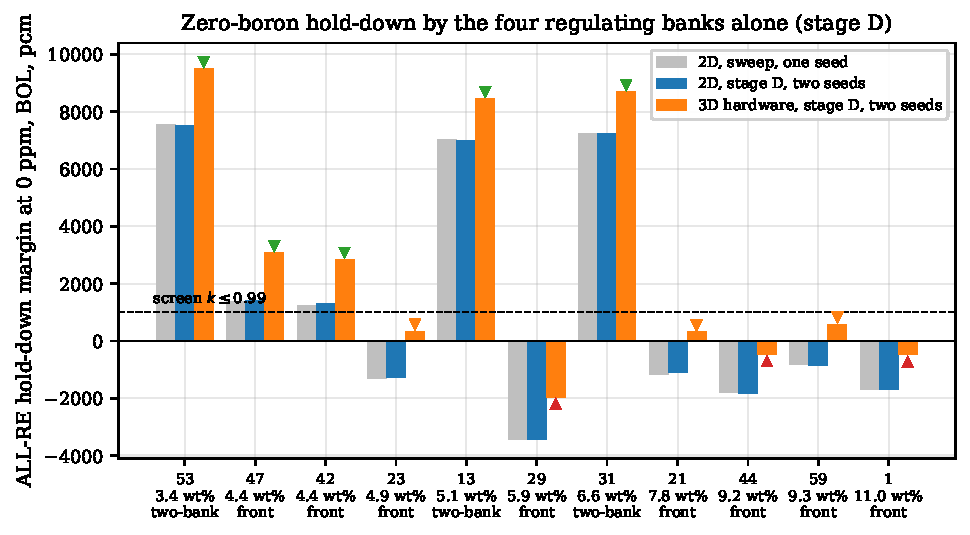
\includegraphics[width=\textwidth]{images/c8_post_zero_boron_margin}
  \caption{Zero-boron hold-down margin under the four regulating banks at beginning of life.}
  \label{fig:c8-post-zero}
\end{figure}

Five designs meet the condition. The three tier B designs hold with
8454 to 9486\,pcm, and the twins 47 and 42 hold with 3069 and
2841\,pcm. Three front members, 23, 21 and 59, are subcritical by only
318 to 581\,pcm, below the margin. Three front members, 29, 44 and 1,
are supercritical under the four banks without boron. No design is
subcritical under RE1 + RE2 alone at 0\,ppm, the two-bank margin there
being $-1162$ to $-11\,757$\,pcm.

Two members of the feasible front satisfy
Equation~\eqref{eq:boronfree-necessary}, designs 47 and 42, at
\SI{3069}{pcm} and \SI{2841}{pcm}. Of the two, design 47 is the
candidate carried forward, because it is also the low-peaking floor of
the front and the only one of the pair whose two-bank status is
resolved beyond the seed uncertainty
(Section~\ref{sec:res-c8-3d}). It is therefore the boron-bearing
candidate of tier A and, at the same time, the design on which a
boron-free variant of the core can be studied.

The three tier B designs hold at zero boron by a wider margin than
either front member, \SIrange{8454}{9486}{pcm} against
\SIrange{2841}{3069}{pcm}, so the design best placed for a boron-free
study is not on the front at all. This is the same inversion reported
in Section~\ref{sec:res-c8-tiers} for controllability, seen now in the
boron budget.

Two limits apply to every statement in this subsection.
Equation~\eqref{eq:boronfree-necessary} is a necessary condition and
not a demonstration, and three things it does not cover are listed in
Section~\ref{sec:res-c8-post-limits}. It is also a four-bank condition
throughout: no design of the eleven is subcritical under RE1 + RE2
alone at \SI{0}{ppm}, so none of these designs is boron-free on the
two-bank state that tier B is defined by.

The one-seed sweep and the two-seed two-dimensional solve agree within
100\,pcm for every design. The three-dimensional core adds 1207 to
1968\,pcm of margin in the rodded state, which is the axial factor of
the rodded core discussed in Section~\ref{sec:res-c8-3d}.

\subsection{Which constraint binds}
\label{sec:res-c8-nesting}

In Campaign 7 the derived ceiling $k_{\max}$ rejected fourteen
controllable designs and the control screen rejected none that the
ceiling accepted. Campaign 8 inverts this. Of the 41 infeasible designs,
six fail $k_{\min}$, 23 fail both $k_{\max}$ and the control screen, and
twelve fail the control screen alone. No design fails $k_{\max}$ alone.
The three-dimensionally derived ceiling of 1.166 is now a redundant
outer bound and the control screen is the binding constraint.
Figure~\ref{fig:c8-post-nesting} shows the structure. In panel~(a) the
twelve designs rejected by the control screen alone are circled in red.
The dashed line is the screen value 0.99, and the dotted lines are
$k_{\min}$ and $k_{\max}$.

\begin{figure}[htbp]
  \centering
  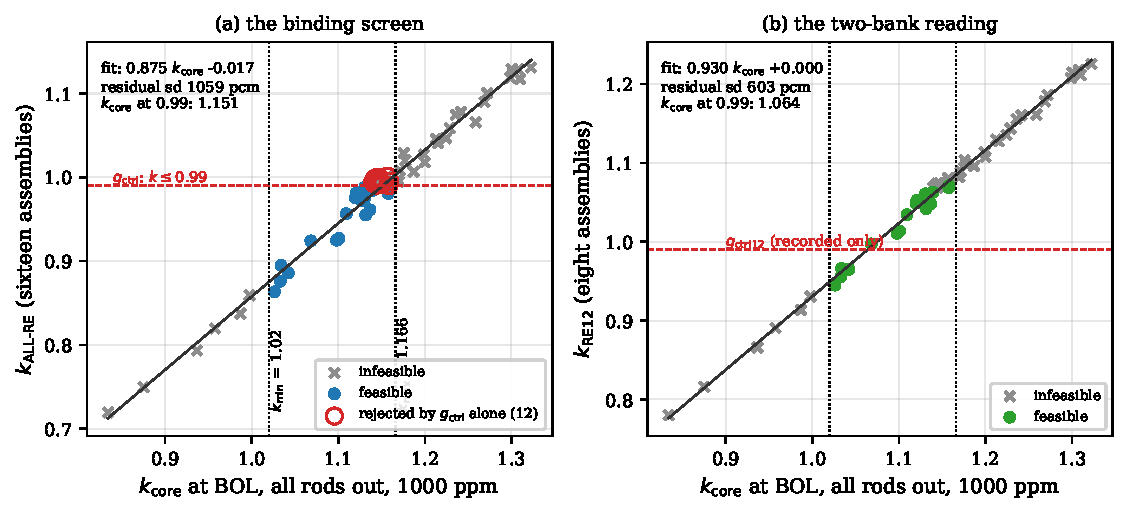
\includegraphics[width=\textwidth]{images/c8_post_constraint_structure}
  \caption[Rodded against unrodded core eigenvalues of the Campaign 8 archive]{Rodded against unrodded core eigenvalues of the 60 Campaign 8 archive designs at 1000\,ppm. (a)~Four-bank state. (b)~Two-bank state.}
  \label{fig:c8-post-nesting}
\end{figure}

A linear fit across the archive gives
$k_\mathrm{RE} = 0.875\,k_\mathrm{core} - 0.017$ with a
residual standard deviation of 1059\,pcm, so the control screen acts
as an effective ceiling near $k_\mathrm{core} = 1.151$, with a spread
that the bank worth of each design sets. For the two-bank state the fit
is $k_\mathrm{RE12} = 0.930\,k_\mathrm{core}$ with a residual of
603\,pcm, and the effective ceiling is $k_\mathrm{core} = 1.064$.

\subsection{Statistical resolution of the front}
\label{sec:res-c8-sigma}

The post-analysis ran every solve with two seeds and the marginal
re-score with three. Table~\ref{tab:c8-post-sigma} pools the seed-to-seed
standard deviations. For the eigenvalue it is 20 to 23\,pcm, equal to
the Monte Carlo standard deviation reported by each solve, so the
reported uncertainty is faithful. For the peaking factor it is 0.011 with
all rods out on the two-dimensional core, pooled over fourteen pairs,
0.012 on the three-dimensional core, whose value is axially integrated,
and 0.024 to 0.029 in the rodded states, whose power distribution is
far more peaked.

\begin{table}[htbp]
  \centering
  \footnotesize
  \caption{Seed-to-seed standard deviation of the post-analysis core solves at $150\,000$ particles, 200 batches and 80 inactive batches.}
  \label{tab:c8-post-sigma}
  \begin{tabular}{@{}l l r r r@{}}
    \toprule
    State & Model & pairs & $\sigma_\mathrm{seed}(k)$, pcm & $\sigma_\mathrm{seed}(F_{\Delta H})$ \\
    \midrule
    RE, 0 ppm & 2D & 11 & 20 & 0.0278 \\
    RE, 0 ppm & 3Dhw & 11 & 23 & 0.0273 \\
    ARO, 1000 ppm & 2D & 14 & 14 & 0.0106 \\
    ARO, 1000 ppm & 3Dhw & 14 & 24 & 0.0119 \\
    \bottomrule
  \end{tabular}
\end{table}

Scaled to the archive fidelity of $100\,000 \times 170$, the
seed-to-seed standard deviation of $F_{\Delta H}$ is about 0.014. The
low-peaking end of the front, designs 47, 42, 23 and 29, spans 1.510 to
1.542 in steps of 0.008 to 0.012, less than one standard deviation
each. These four designs are ordered by cycle length but not by
peaking. Any statement that ranks them by $F_{\Delta H}$ requires a
replicate of at least four seeds at 1000\,ppm with all rods out, which
brings the standard error of each mean to about 0.006, the size of the
smallest step.

The re-score of designs 54 and 11 with three seeds gives
$k_\mathrm{RE} = 0.99038 \pm 54$ and $0.99053 \pm 25$\,pcm.
Both are subcritical and both remain above the screen value 0.99, by
38 and 53\,pcm, so the feasibility count stays at 19. Both are dominated
on the objectives, 54 by 21 and 44, and 11 by 44, so the front is
unchanged either way.

\subsection{Three-dimensional closures}
\label{sec:res-c8-3d}

The axial factor of the rodded core differs from that of the unrodded
core. With all rods out the three-dimensional core model gives
$L_\mathrm{ax} = k_\mathrm{2D} / k_\mathrm{3D}$ between 1.0286 and
1.0311 at 1000\,ppm over the eleven confirmed designs, against the 1.0282
to 1.0298 of the water-slab axial study of Section~\ref{sec:meth-lax}.
With RE1 + RE2 inserted it is between 1.0219 and 1.0252, and with the
four regulating banks inserted between 1.0126 and 1.0177. The reason is
the rod stack.
The two-dimensional screen inserts B$_4$C over the whole fuel height,
whereas the benchmark rod leaves the bottom 12.04\,cm of the fuel
unrodded, carries 30.48\,cm of Ag-In-Cd above it and B$_4$C over the
remaining 77.48\,cm. The three-dimensional rodded core is therefore
less rodded than the two-dimensional one, and part of the axial leakage
gain is spent on the weaker stack, in proportion to the number of rods
inserted. The two-dimensional control screen remains conservative, by
\num{1272} to \SI{2047}{pcm} for the four-bank state and by \num{2062}
to \SI{2671}{pcm} for the two-bank state, rather than by the 2900 to
3100\,pcm that the unrodded axial factor would suggest. Both ranges are
the differences of the margin columns of
Table~\ref{tab:c8-post-3d1000} over the eleven confirmed designs. The
two-dimensional eigenvalues of the confirmation reproduce the archive
within $-53$ to $+69$\,pcm over the thirty-three comparisons.

The unrodded axial factor splits by enrichment. The six designs at or
below \SI{5.90}{wt\%} give 1.0301 to 1.0311 and the five at or above
\SI{6.59}{wt\%} give 1.0286 to 1.0291. The campaign value 1.0289 is
therefore right for the long-cycle designs and 120 to 220\,pcm low for
the low-peaking end of the front.
%% AUTHOR: physics of the split. Two mechanisms are candidates, the
%% parked-rod plug at the fuel top weighing more where the competing
%% absorption is lower, and the migration area of the softer spectrum.
%% Stage E on design 47 isolates the first at 129 pcm, so the second
%% accounts for the remainder of the 130 to 220 pcm. State which you
%% adopt, or leave the observation as measured.

The parked rods matter. With the withdrawn rods removed from the model,
design 47 gives $L_\mathrm{ax} = 1.0291$, within 20\,pcm of the
campaign value 1.0289 taken from the water-slab axial study. With the
rods parked in the benchmark position the factor is 1.0304, a
difference of 129\,pcm, because the withdrawn rod leaves its steel end
plug in the top 4.86\,cm of the fuel and its Ag-In-Cd tip in the
plenum above. The parked geometry therefore raises the end-of-cycle
target by about 130\,pcm, which shortens the reported cycle of design
47 by about 24\,EFPD, or 1.2\,\%, on the slope of its reactivity
history, and the long cycles by a smaller fraction.

The downcomer trade is nearly free. Thinning the reflector of designs
47, 21 and 59 to 3.969\,cm, which gives a 3.7\,cm downcomer at the
1.26\,cm pitch, changes the unrodded two-dimensional eigenvalue by
$-5$, $-95$ and $-128$\,pcm and the peaking factor by $+0.003$ to
$+0.005$, below one seed standard deviation.
Table~\ref{tab:c8-post-downcomer} gives the values. The native column
is the archive core solve at $100\,000 \times 170$, and $\Delta\rho$ is
the reactivity change of the two-dimensional core. A downcomer of
3.7\,cm can be adopted for every candidate at a cost of at most
130\,pcm at beginning of life.

\begin{table}[htbp]
  \centering
  \footnotesize
  \caption{Stage G: reflector thinned to 3.969\,cm for a 3.7\,cm downcomer at pitch 1.26\,cm, all rods out, 1000\,ppm, two seeds.}
  \label{tab:c8-post-downcomer}
  \setlength{\tabcolsep}{3pt}\scriptsize
  \begin{tabular}{@{}l r r r r r r r@{}}
    \toprule
    ID & $t_\mathrm{refl}$ & downcomer & $k_\mathrm{2D}$ & $k_\mathrm{2D}$ & $\Delta\rho$ & $F_{\Delta H}$ & $F_{\Delta H}$ \\
       & native, cm & native, cm & native & at 3.969 & pcm & native & at 3.969 \\
    \midrule
    47 & 4.29 & 3.38 & 1.0981 & 1.0980 & -4 & 1.510 & 1.513 \\
    21 & 4.92 & 2.75 & 1.1264 & 1.1253 & -82 & 1.592 & 1.595 \\
    59 & 5.66 & 2.01 & 1.1198 & 1.1186 & -102 & 1.634 & 1.639 \\
    \bottomrule
  \end{tabular}
\end{table}

\subsection{The reflector inside the Campaign 8 box}
\label{sec:res-c8-refl}

Campaign 3 found the radial peaking of the core to fall with reflector
thickness over the 2 to 19.5\,cm range. Inside the 2.0 to 5.66\,cm box
of Campaign 8 the effect is not resolved. A multiple regression of
$F_{\Delta H}$ on the four design variables over the 60 designs gives
$-0.0085$ per centimetre, that is $-0.031$ across the box, and the
subset below 7\,wt\% gives the opposite sign. The direct test of
Section~\ref{sec:res-c8-3d} measures at most $+0.005$ for a thinning of
0.3 to 1.7\,cm. Figure~\ref{fig:c8-post-refl} shows both, with the
designs coloured by enrichment, circles for the feasible designs and red
arrows for the stage G solves with the reflector thinned to 3.969\,cm.

\begin{figure}[htbp]
  \centering
  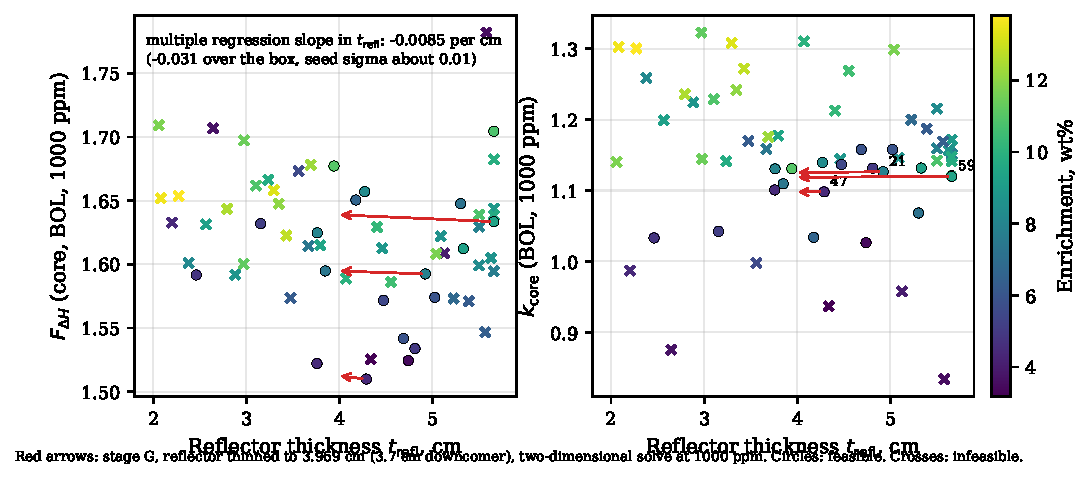
\includegraphics[width=\textwidth]{images/c8_post_reflector_leverage}
  \caption{Peaking factor and unrodded core eigenvalue against reflector thickness, 60 Campaign 8 archive designs.}
  \label{fig:c8-post-refl}
\end{figure}

Within this box the reflector thickness is therefore nearly inert. It
carries about 52\,pcm per centimetre of reactivity through the target of
Section~\ref{sec:meth-lax} and a peaking effect of the order of the
solve noise. Two consequences follow.

\begin{enumerate}
  \item The infill separation criterion, measured in the normalised
        design space, admitted the twins 47 and 42 on the strength of
        the reflector coordinate alone. A separation criterion in
        objective space, or a smaller weight on inert coordinates, would
        have spent that evaluation elsewhere.

  \item Any further campaign in this box should fix the reflector at
        3.97\,cm, which gives the 3.7\,cm downcomer, and search the three
        active variables.
\end{enumerate}

\subsection{Moderator temperature coefficient and the boron ceiling}
\label{sec:res-c8-mtc}

The boron sweep and the swing table give the critical concentration of
each candidate, and Section~\ref{sec:meth-mtc} defines the ceiling that
concentration has to stay below at power. The ceiling was measured on
C8-47, and Table~\ref{tab:c8-mtc} gives its two-dimensional screen and
its value on the three-dimensional core model at the two primary
conditions.

\begin{table}[htbp]
  \centering
  \small
  \caption{C8-47, zoned core: soluble boron ceiling at two primary conditions.}
  \label{tab:c8-mtc}
  \begin{tabular}{@{}rcrrrr@{}}
    \toprule
    Pressure & Bracket & 2D screen & 3D result & 3D weighted fit & 3D margin on 2327\,ppm \\
    {[MPa]} & [K] & [ppm] & [ppm] & [ppm] & [ppm] \\
    \midrule
    15.5 & 570 to 590 & 2336 & 2997 & $2981 \pm 61$ & $+670$ \\
    12.8 & 547 to 567 & 2255 & 2763 & $2762 \pm 70$ & $+436$ \\
    \bottomrule
  \end{tabular}
\end{table}

The ceilings are the two-point values of Section~\ref{sec:meth-mtc}, and
a weighted linear fit over the scanned concentrations agrees with the
three-dimensional values within one standard deviation at both
pressures. The Doppler coefficient is negative and resolved throughout,
from $-2.15$ to \SI{-1.79}{pcm} per K at \SI{15.5}{MPa} and from
$-2.08$ to \SI{-1.85}{pcm} per K at \SI{12.8}{MPa}, so the temperature
interpolation is active. The axial leakage contribution of
Equation~\eqref{eq:axial-feedback} is $-10.63 \pm 0.55$\,pcm per K, 29
per cent of the total coefficient of the three-dimensional core at the
conditions of the scan, and it raises the ceiling by \SI{661}{ppm} at
\SI{15.5}{MPa} and by \SI{508}{ppm} at \SI{12.8}{MPa}.

Design 47 itself needs \SI{2327}{ppm} at beginning of life, measured
as the root of its zoned reactivity curve at \SI{570}{K} with the
state offset of \SI{157}{pcm} between the scan and the campaign
operating point applied. The linear estimate of
Table~\ref{tab:c8-swing} is \SI{2348}{ppm}. Its hump is negative, so
beginning of life is its most reactive state, and it clears the
three-dimensional ceiling by \SI{670}{ppm} at \SI{15.5}{MPa} and
\SI{436}{ppm} at \SI{12.8}{MPa}. Under the two-dimensional screen it is
marginal at \SI{15.5}{MPa}, \SI{9}{ppm} below 2336, and fails at
\SI{12.8}{MPa}, \SI{72}{ppm} above 2255, a difference that the axial
term of Section~\ref{sec:meth-mtc-3d} accounts for. The estimates of Table~\ref{tab:c8-swing} place the
other candidates as follows, with the caution that the ceiling was
measured on the lattice of design 47 only.

\begin{enumerate}
  \item Designs 53, 13 and 42 need 1312, 1697 and \SI{2377}{ppm}, all
        with a negative hump, and lie below both ceilings. A second
        record of design 13 gives \SI{1701}{ppm}, a difference below
        the resolution of the estimate.

  \item Design 31 needs \SI{1701}{ppm} at beginning of life and
        \SI{2760}{ppm} at the maximum of its hump, \SI{3}{ppm} below the
        three-dimensional ceiling at \SI{12.8}{MPa}.

  \item Design 23 needs \SI{2979}{ppm}, \SI{18}{ppm} below the
        three-dimensional ceiling at \SI{15.5}{MPa} and above the one at
        \SI{12.8}{MPa}.

  \item The five long-cycle members of the front, 29, 21, 59, 44 and 1,
        need 3677 to \SI{4674}{ppm} at beginning of life, above both
        ceilings.
\end{enumerate}

Boron control at a non-positive coefficient is therefore available to
the short-cycle end of the front and to the two-bank subset, and not
to the long-cycle designs. This is the same division that the
controllability readings of Sections~\ref{sec:res-c8-tiers}
and~\ref{sec:res-c8-zeroboron} drew.

\subsection{The proxy gap on the zoned core}
\label{sec:res-proxy-gap-zoned}

The bridge model of Equation~\eqref{eq:bridge} was fitted in
Section~\ref{sec:res-corevalidation} on the uniform-loading archive of
Campaign~3, where it identified the reflector thickness and the pin
pitch as the variables that set the ratio between the core and the
assembly peaking factor. From Campaign~6 the evaluator builds the zoned
core of Section~\ref{sec:meth-zoning}, and every archive from
Campaign~4 onward stores both peaking factors of each design, the core
value as the objective and the assembly value as the diagnostic of
Section~\ref{sec:meth-core-objective}. The fit can therefore be
repeated on the zoned core without new transport.

Table~\ref{tab:proxy-gap-zoned} compares the four archives. The
Campaign~3 row is not a sample mean: it is
Equation~\eqref{eq:bridge-fit} evaluated at the operating point of
Campaign~8, $p = \SI{1.26}{cm}$ and $t_\mathrm{refl} = \SI{4.0}{cm}$.
The regression cannot be fitted on the Campaign~8 archive, whose pitch
is fixed, so only the mean ratio is given for it. The zoned ratios were
computed from the archived core and assembly peaking factors of the
Campaign~6, 7 and 8 checkpoints.

\begin{table}[htbp]
  \centering
  \small
  \caption{Uniform and zoned archives: ratio of the core to the assembly peaking factor.}
  \label{tab:proxy-gap-zoned}
  \begin{tabular}{@{}llrcrr@{}}
    \toprule
    Archive & Loading & $n$ & Pitch & $F_{\Delta H}^\mathrm{core}/F_{\Delta H}^\mathrm{asm}$ & $R^2$ of \\
     &  &  & [cm] & mean $\pm$ sd & Eq.~\eqref{eq:bridge} \\
    \midrule
    Campaign 3 & uniform & 36  & 1.15 to 1.43 & 1.814 (fit) & 0.746 \\
    Campaign 6 & zoned   & 114 & 1.15 to 1.43 & $1.318 \pm 0.052$ & 0.030 \\
    Campaign 7 & zoned   & 60  & 1.15 to 1.41 & $1.297 \pm 0.035$ & 0.052 \\
    Campaign 8 & zoned   & 60  & 1.26 fixed   & $1.313 \pm 0.029$ & -- \\
    \bottomrule
  \end{tabular}
\end{table}

Three readings follow.

\begin{enumerate}
  \item The ratio is much smaller on the zoned core. The Campaign~3 fit
        predicts 1.814 at the Campaign~8 operating point, and the
        Campaign~8 archive gives 1.313. The quotient of the two, 1.38,
        lies within the peaking reduction measured directly on two
        Campaign~5 champions in Table~\ref{tab:zoning-confirm}, where
        zoning lowered $F_{\Delta H}$ from 2.026 to 1.501 and from 2.043
        to 1.473, factors of 1.35 and 1.39. The archive comparison and
        the controlled comparison give the same zoning benefit.

  \item The geometric dependence is lost. On the uniform core the two
        regressors of Equation~\eqref{eq:bridge} explain three quarters
        of the variance of the ratio. On the Campaign~6 archive, over
        the same pitch range and with three times as many designs, they
        explain 3 per cent, and 5 per cent on Campaign~7. Within its
        scatter, the ratio on the zoned core depends on neither the
        reflector thickness nor the pitch.

  \item The ratio is stable between campaigns. The three zoned archives
        give 1.318, 1.297 and 1.313, a spread of 0.021, smaller than
        the standard deviation within each archive, 0.029 to 0.052,
        over 234 designs and three different design spaces.
\end{enumerate}

The zoning was designed to remove this dependence. The assembly
calculation has reflective boundaries, so it describes an infinite
lattice of identical assemblies and measures only the pin-to-pin
structure inside one assembly, 1.14 to 1.15 on the uniform Campaign~3
finalists of Table~\ref{tab:core-finalists}. The core calculation keeps
that structure and multiplies it, approximately, by the radial form
factor, the ratio of the power of the hottest assembly to the core
mean. On the uniform core the form factor is large and depends on the
geometry, because the reflector and the pitch set how steeply the power
falls toward the periphery. The zoned map enriches the periphery and
derates the centre while the fissile balance of
Equation~\eqref{eq:zoning-balance} holds the mean multiplier at one,
and the form factor that results is smaller and insensitive to the two
geometric variables.

Two consequences follow for the method.

\begin{enumerate}
  \item The Campaign~4 decision to measure the core peaking inside the
        loop holds on the zoned core as well. A constant ratio with a
        relative scatter of 2.2 per cent on Campaign~8 corresponds to
        about 0.036 in the core peaking factor. That is between two and
        three times the seed-to-seed standard deviation of the core
        solve at the archive fidelity, about 0.014
        (Section~\ref{sec:res-c8-sigma}), and larger than the steps of
        0.008 to 0.012 between the low-peaking designs of the front. A
        corrected assembly value would place a design in the right
        region of the objective plane but could not order the front on
        the peaking axis, and at 3 per cent of an evaluation the
        measurement is the cheaper choice.

  \item Outside the loop, for screening, the assembly peaking predicts
        the core peaking of the zoned core through a single calibrated
        factor. The leakage-corrected reactivity target of
        Section~\ref{sec:meth-ktarget} has the same property for the
        multiplication factor: an assembly calculation carries the core
        behaviour once a correction that is stable over the design
        space is applied.
\end{enumerate}

The archive does not decide between a multiplicative and an additive
correction. On Campaign~8 the ratio has a relative standard deviation
of 2.2 per cent and the difference
$F_{\Delta H}^\mathrm{core} - F_{\Delta H}^\mathrm{asm}$ is
$+0.386 \pm 0.033$. Expressed in units of the core peaking factor the
two scatters are of the same size, 0.03 to 0.04, because the archive
spans a narrow range of peaking factors. The multiplicative form of
Equation~\eqref{eq:bridge} is kept because the mechanism described
above is the product of a local and a radial factor, and an additive
offset fitted on this narrow range would not transfer to a core with a
different local peaking.

\subsection{Limitations of the post-analysis}
\label{sec:res-c8-post-limits}

\begin{enumerate}
  \item Every margin is a beginning-of-life value on fresh, xenon-free
        materials. The gadolinia burns out during the first part of the
        cycle and $k_\infty$ may rise before it falls. The minimum
        hold-down margin over the cycle may then sit at that maximum. The
        depletion histories of the eleven designs are on disk and the
        maximum can be located without new transport.
        The operating maximum was located from those histories in
        Section~\ref{sec:res-c8-closures}, where the hump of $-1723$ to
        $+4955$\,pcm on the core is applied to the margins before the
        candidate decision.

  \item The cycle lengths of the archive are those of a core held at
        1000\,ppm for the whole cycle, because the depleting assembly
        carries the operating point of the core solve. Both a boron
        letdown cycle and a boron-free cycle reach end of cycle with the
        absorber removed, so every reported cycle length is a lower bound.
        The bias is larger for the low-enrichment designs, whose boron
        worth is higher.
        \openpoint{Deplete design 47 at 0\,ppm with the same schedule, and
        recompute the reference target at 0\,ppm with one assembly and
        one core solve, to measure the bias on the boron-free candidate.}

  \item Equation~\eqref{eq:boronfree-necessary} is necessary and not
        sufficient for boron-free operation. It does not cover the
        cold-shutdown margin with the highest-worth rod stuck out, which
        needs the shutdown bank positions and a temperature-dependent
        water density that the model does not have, and it does not cover
        the power-shape penalty of operating with regulating banks
        partly inserted through the cycle.

  \item The boron sweep is a single-seed study. Its eigenvalues are
        confirmed by the two-seed solves of stage D at 0\,ppm and by the
        archive at 1000\,ppm, but its rodded peaking factors carry the
        0.028 seed noise of Table~\ref{tab:c8-post-sigma} and are not
        used for any conclusion.

  \item Discharge burnups of 50 to 58\,MWd/kgHM core average, as reached
        by designs 44, 59 and 1, combine with the 1.15 periphery
        multiplier and the radial peaking into peak-pin burnups that the
        screens do not bound.
        %% AUTHOR: state the fuel-performance basis you adopt for the
        %% discharge burnup and whether it removes 44, 59 and 1 from the
        %% candidate list. This is the physical argument that separates
        %% tier A from tier B in the candidate decision.
\end{enumerate}

\subsection{Candidate decision}
\label{sec:res-c8-decision}

Design 47 is the candidate carried forward, because it satisfies the
three readings of the post-analysis at once. It is the low-peaking
floor of the feasible front, at 1941\,EFPD, $F_{\Delta H} = 1.510$ and
4.39\,wt\% assembly enrichment. It is controllable with the first two
regulating banks at 1000\,ppm on the three-dimensional core, with a
margin of 1330\,pcm that survives the gadolinium hump because its
beginning of life is its most reactive state
(Table~\ref{tab:c8-swing}). And it satisfies the necessary condition
for boron-free operation of Equation~\eqref{eq:boronfree-necessary},
holding 3069\,pcm under the four regulating banks at 0\,ppm, one of
only two front members that do, the other being its twin 42 at
2841\,pcm, whose two-bank status the seed noise does not resolve.

Its cycle length is the shortest on the front, and the short cycle is
a cost relative to the rest of the front and not a shortfall against
the reference envelope: 1941\,EFPD is 6.6 calendar years at a capacity
factor of 0.8, above the five years reported for the
prototype (Section~\ref{sec:res-c8-mission}). The physical reason the
same design leads all three readings is the one stated in
Section~\ref{sec:res-c8-split}. Every reading rewards a small
beginning-of-life excess, and the design at the low-enrichment end of
the front carries the smallest excess that still meets the mission.

Two alternatives are recorded for a decision that weighs cycle length
more heavily. With boron, design 21 at the knee of the front gives
4221\,EFPD at $F_{\Delta H} = 1.592$ and 7.81\,wt\%, controllable by
the four banks only and not boron-free. Under two-bank control, design
31 gives 3381\,EFPD at $F_{\Delta H} = 1.650$ and 6.59\,wt\%, the
enrichment reported for the prototype in 2014, holding 5856\,pcm with
two banks on the three-dimensional core at beginning of life and
8684\,pcm boron-free under four banks, but its hump of 4955\,pcm
removes the two-bank margin at the operating maximum
(Section~\ref{sec:res-c8-closures}).

Design 47 is the candidate of the Campaign 8 formulation. Scored on the
objectives of Campaign 9 it is dominated by members of the Campaign 9
front, as Section~\ref{sec:res-c9-compare} shows.

\subsection{Retrospective scoring of the reformulated problem}
\label{sec:res-c8-retro}

Before Campaign 9 was launched, the reformulation of
Section~\ref{sec:concl-reform} was scored on the archives of
Campaigns 7 and 8 with no transport, using
\texttt{c8\_reformulation\_retro.py}, in two parts.

The first part applies the control screen at the operating maximum of
each depletion history instead of at beginning of life. On the 58
scored Campaign 7 designs the screen then passes 32 designs against 38
at beginning of life, and removes designs 11, 48, 49, 53, 54 and 55. On
Campaign 8 it changes the verdict of design 31 alone.

The second part minimises $F_{\Delta H}$ and the critical boron
concentration at the operating maximum on the Campaign 8 archive,
subject to a cycle-length floor and to $F_{\Delta H} \le 1.65$. With
no measured concentration outside the eleven post-analysis designs, the
concentration is estimated from a boron-worth law fitted on those
eleven.

\begin{equation}
w_\mathrm{B}(e) = 23.292\, e^{-0.8496}
\label{eq:wb-proxy}
\end{equation}

\noindent where the symbols have the following meaning.

\begin{itemize}
  \item $w_\mathrm{B}$ is the differential boron worth, in pcm per ppm.

  \item $e$ is the assembly enrichment, in wt\%.
\end{itemize}

The fit has a relative root-mean-square residual of \SI{1.6}{\%}, and
its largest error on a critical concentration is \SI{138}{ppm}. The
concentration is scored at the operating maximum, humps below
\SI{400}{pcm} are set to zero, the measured rodded screen is used
where a measurement exists, and a design whose score depends on an
extrapolation of the law is flagged. Table~\ref{tab:c8-retro} gives
the front at three floors.

\begin{table}[htbp]
  \centering
  \small
  \caption{Campaign 8 archive, reformulated problem: front at three cycle-length floors.}
  \label{tab:c8-retro}
  \begin{tabular}{@{}rll@{}}
    \toprule
    Floor [EFPD] & Calendar interval & Front (Campaign 8 designs) \\
    \midrule
    1826 & five years at a capacity factor of one & 13, 47 \\
    2557 & seven years & 22, 40, 51 \\
    2922 & eight years & 19, 22, 36, 43, 51 \\
    \bottomrule
  \end{tabular}
\end{table}

The five-year front is the only one whose members all carry a measured
control margin, a three-dimensional confirmation and a measured
critical concentration. The longer fronts rest on extrapolations of
Equation~\eqref{eq:wb-proxy}, flagged for designs 43 and 51. The floor
of 1826\,EFPD was adopted for Campaign 9, and the boron worth was
measured on every design there instead of estimated.


\section{Campaign 9: the reformulated objective set}
\label{sec:res-c9}

Campaign 8 closed with a question. The controllability constraint, and
not the cycle length, decided which designs survived, and the
retrospective of Section~\ref{sec:res-c8-retro} showed that an objective
set built around the soluble boron requirement would select a different
part of the archive. Campaign 9 runs that formulation instead of
inferring it.

The campaign changes the formulation of Section~\ref{sec:meth-c9} and
keeps everything else. The design space, the transport fidelity, the
depletion schedule, the leakage-corrected target and the zoned loading map
of Section~\ref{sec:meth-zoning} are those of Campaign 8, so a difference
in outcome is attributable to the reformulation. Design indices from this
section onward carry the prefix of their campaign: C9-47 and C8-47 are
different designs that happen to share an archive index.

\subsection{Measurement and cost}
\label{sec:res-c9-formulation}

The objectives are $F_{\Delta H}$ and the critical boron concentration at
the operating maximum, Equations~\eqref{eq:c9-problem}
and~\eqref{eq:c9-cmax}. The control screen is applied at the operating
maximum through Equation~\eqref{eq:margin-peak}, and the guards that clamp
the objective at \SI{0}{ppm} and clip it at \SI{6000}{ppm} are those of
Section~\ref{sec:meth-c9}. The boron worth is measured in every evaluation
and is not taken from the power law of Equation~\eqref{eq:wb-proxy}.

That measurement also tests the correlation it replaces. The power law was
fitted on eleven Campaign 8 designs, and Campaign 9 measures the worth of
sixty, an independent sample more than five times larger than the fit.
Figure~\ref{fig:c9-wb-proxy} compares the two: the upper panel draws the
worth against enrichment, and the lower panel the relative residual of the
law with its root-mean-square band shaded. The relative root-mean-square
deviation is \SI{3.5}{\%} with a mean bias of \SI{-1.2}{\%}, and the
agreement is not uniform. Below \SI{5.6}{wt\%}, where every feasible design
lies, the bias is \SI{-0.3}{\%} and the scatter \SI{2.6}{\%}. Above that
value the law overestimates the worth by \SI{3.6}{\%} on average. Two
consequences follow, and they point in opposite directions.

\begin{enumerate}
  \item Inside the converged region the correlation would have been
        adequate. A \SI{2.6}{\%} error in the worth is a \SI{2.6}{\%} error
        in the concentration, about \SI{45}{ppm} at \SI{1700}{ppm}, against
        a front that spans \SI{502}{ppm}, so the ranking of the front would
        not have changed.

  \item Outside it the correlation degrades where the archive is most
        uncertain. The high-enrichment designs whose concentration reaches
        the clip are the ones the law overestimates, so a
        correlation-driven campaign would have compounded an extrapolated
        worth with an extrapolated root. Measuring removes that compounding
        at a cost of \SI{14.5}{\%} of the campaign.
\end{enumerate}

\begin{figure}[htbp]
  \centering
  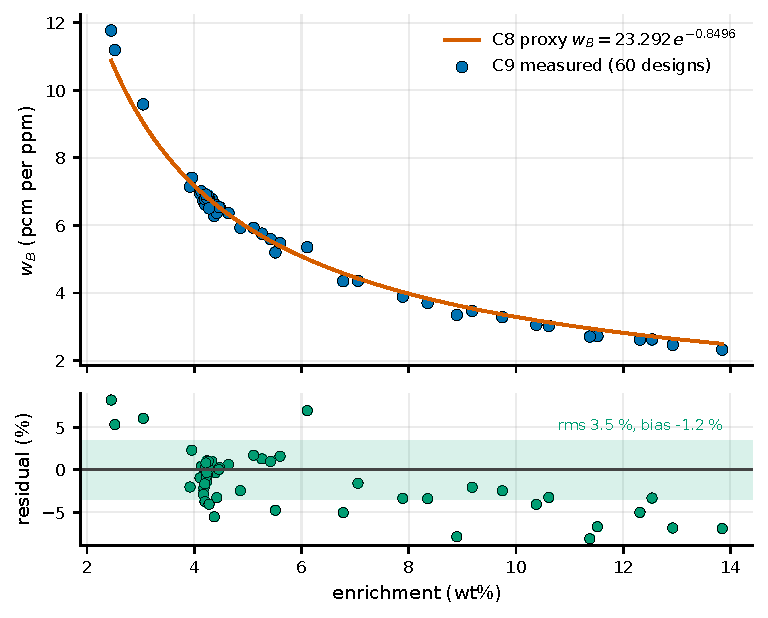
\includegraphics[width=0.80\textwidth]{c9_wb_proxy}
  \caption{Campaign 9, 60 designs: measured differential boron worth against the Campaign 8 power law.}
  \label{fig:c9-wb-proxy}
\end{figure}

The campaign ran 60 evaluations in \SI{18.65}{h} on the reference
workstation, and the boron measurement took \SI{2.71}{h} of that,
\SI{14.5}{\%}, at one or two extra core solves per design. That is five
times the \SI{3}{\%} increment that moved the peaking objective to core
level in Campaign 4. Figure~\ref{fig:c9-cost} separates the total: the
left panel gives the aggregate wall time by component, and the right panel
the wall time of each evaluation, separated by the number of boron solves,
with the design of experiments shaded. Depletion at assembly level takes
\SI{10.47}{h}, \SI{56}{\%} of the campaign, and the three core solves of
the screens and of the reference concentration take \SI{5.28}{h} together.
The new measurement is therefore not the expensive part of an evaluation,
because of the adaptive bracket. Ninety boron solves were needed for sixty
designs, 1.5 per design, since a single solve at \SI{2000}{ppm} already
brackets the root whenever the design is near criticality at the reference
concentration. The designs that needed a second solve are the
high-enrichment ones that the constraint set rejects in any case, visible
in the right panel as the group near 30 minutes inside the design of
experiments.

\begin{figure}[htbp]
  \centering
  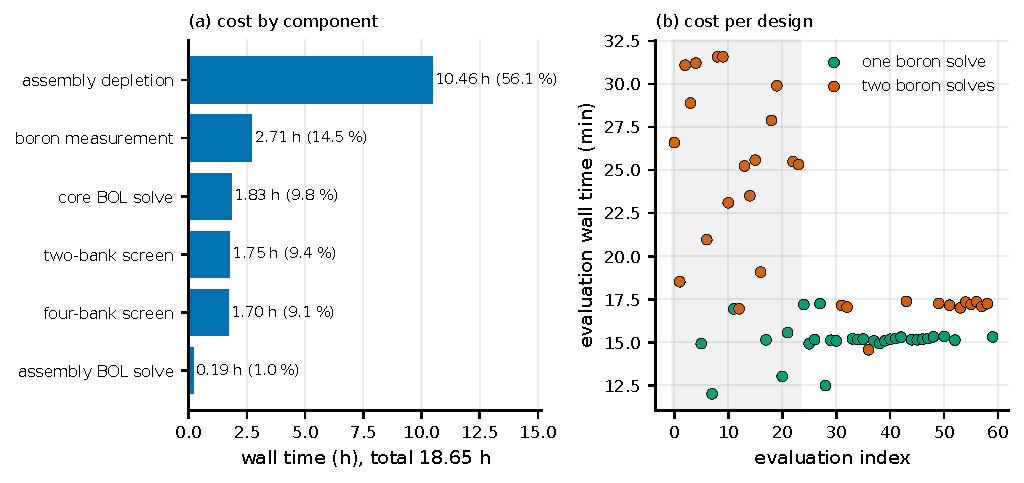
\includegraphics[width=\textwidth]{c9_cost}
  \caption{Campaign 9: wall time by component and per evaluation.}
  \label{fig:c9-cost}
\end{figure}

\subsection{The feasible set and the Pareto front}
\label{sec:res-c9-front}

Of the 60 designs evaluated, 22 satisfy every constraint, and 20 of those
need less boron than the ceiling of C9-47, \SI{2897}{ppm} at
\SI{12.8}{MPa} in three dimensions (Section~\ref{sec:res-c9-ceiling}).
That ceiling belongs to one lattice and serves here only as a reference
line, because Section~\ref{sec:res-c9-ceiling} shows that every design has
its own. Thirteen of the 22 pass the two-bank screen of Campaign 8, a
two-dimensional reading at \SI{1000}{ppm}. The Pareto front holds five
designs, listed in Table~\ref{tab:c9-front}. Every concentration in the
table is interpolated between measured points, and the last column is the
two-bank reading at the operating maximum, recorded and not constrained.

\paragraph{Controllability measured where the design operates.}
The two-bank reading carried through the campaign is evaluated on a
two-dimensional core at a fixed \SI{1000}{ppm}, which is neither the
geometry nor the concentration of the operating state. The front was
therefore re-solved on the three-dimensional core model of Section~\ref{sec:res-c8-3d},
at each design's own critical boron, in three states: all rods out, all
rods in, and the first two regulating banks inserted.

At their own critical concentration the five front designs give an
unrodded multiplication factor of 0.97014 to 0.97111 on the three-dimensional core model.
With the first two banks inserted the factor falls to 0.90453 to 0.90713,
a worth of 7263 to \SI{7495}{pcm}, and with all four banks to 0.83819 to
0.84231, a worth of 15\,746 to \SI{16245}{pcm}. Three readings follow:

\begin{enumerate}
  \item Every front member is held subcritical by the first two banks alone,
        with 9228 to \SI{9545}{pcm} of margin against the 0.99 screen of
        Section~\ref{sec:meth-core-objective}. The two-bank capability of
        these designs is roughly nine times what the screen demands.

  \item The two-dimensional screen overstates the bank worth by 4 to
        \SI{7}{\%}. The same two banks are worth 7651 to \SI{7812}{pcm} in
        two dimensions against 7263 to \SI{7495}{pcm} on the three-dimensional core model,
        because the axial reflector and the parked rods change the flux shape
        the banks see. The screen is therefore optimistic, and it remains
        usable because the margin it screens is an order of magnitude larger
        than the error.

  \item The spread across the front is small. The two-bank worth varies by
        \SI{3}{\%} over designs whose gadolinia loading varies by a factor of
        1.7, so the absorber loading has little influence on the bank worth
        at the concentrations these designs run at.
\end{enumerate}

The same measurement on the thirteen two-bank designs at \SI{1000}{ppm}
gives a four-bank worth of 15\,283 to \SI{16285}{pcm}. In the unrodded
state it also gives the axial factor, the ratio of the two-dimensional to
the three-dimensional multiplication factor, of 1.0298 to 1.0312,
consistent with the 1.0289 of Campaign 6 and with the 1.0304 of the
parked-rod study of Section~\ref{sec:res-c8-3d}. This factor is measured at
beginning of life only, because no depletion was run in three dimensions.

\begin{table}[htbp]
  \centering
  \caption{Campaign 9 Pareto front in $(F_{\Delta H}, c_\mathrm{max})$, sorted by boron demand.}
  \label{tab:c9-front}
  \small
  \begin{tabular}{@{}lrrrrrrrrc@{}}
    \toprule
    Design & $e$ & Gd$_2$O$_3$ & pins & $t_\mathrm{refl}$ & EFPD &
    $F_{\Delta H}$ & $c_\mathrm{BOL}$ & $c_\mathrm{max}$ & two \\
     & wt\% & wt\% & & cm & d & & ppm & ppm & banks \\
    \midrule
    C9-47 & 4.46 & 4.42 & 20 & 5.66 & 1947 & 1.545 & 1406 & 1406 & yes \\
    C9-44 & 4.24 & 3.15 & 20 & 5.66 & 1858 & 1.539 & 1334 & 1496 & yes \\
    C9-34 & 4.26 & 3.32 & 16 & 5.66 & 1841 & 1.496 & 1725 & 1725 & yes \\
    C9-40 & 4.23 & 2.71 & 16 & 5.66 & 1870 & 1.495 & 1768 & 1768 & yes \\
    C9-35 & 4.36 & 2.63 & 16 & 5.65 & 1938 & 1.490 & 1908 & 1908 & yes \\
    \bottomrule
  \end{tabular}
\end{table}

Four readings follow.

\begin{enumerate}
  \item The front is narrow. It spans 0.055 in $F_{\Delta H}$ and
        \SI{502}{ppm} in $c_\mathrm{max}$, and every member lies between
        4.23 and \SI{4.46}{wt\%}. The reformulated problem offers a much
        smaller trade than the cycle-length formulation did.

  \item The reflector is at its upper bound of \SI{5.66}{cm} on every
        member, and the tightest vessel-fit value in the archive is
        $g_\mathrm{geom} = \SI{-0.009}{cm}$. The limit is set by the
        \SI{90}{cm} vessel inner radius, and the front uses every
        centimetre of reflector the vessel permits.

  \item The whole front is two-bank controllable at the operating maximum
        on the two-dimensional core. In Campaign 8 three designs of sixty
        met that reading, 12, 13 and 53 once design 31 had lost its margin
        to its hump, and none of them was on the front. The reformulation
        moves the front into the controllable region.

  \item Every front concentration is bracketed by measured points, so no
        front value depends on an extrapolated boron worth.
\end{enumerate}

The second reading holds over the whole campaign, not only on the front.
Figure~\ref{fig:c9-design-space} follows each design variable along the
evaluation order, with the box bounds dotted, the design of experiments
shaded and the feasible designs filled. The reflector reaches its bound at
the first infill iteration and stays there, and the enrichment collapses
from the full 2.0 to \SI{13.9}{wt\%} box to a band narrower than
\SI{0.5}{wt\%} around \SI{4.3}{wt\%}. The gadolinia content and the pin
count stay spread over most of their ranges to the last evaluation, so the
optimiser found no single best absorber loading and trades it against the
peaking objective inside an otherwise fixed design.

\begin{figure}[htbp]
  \centering
  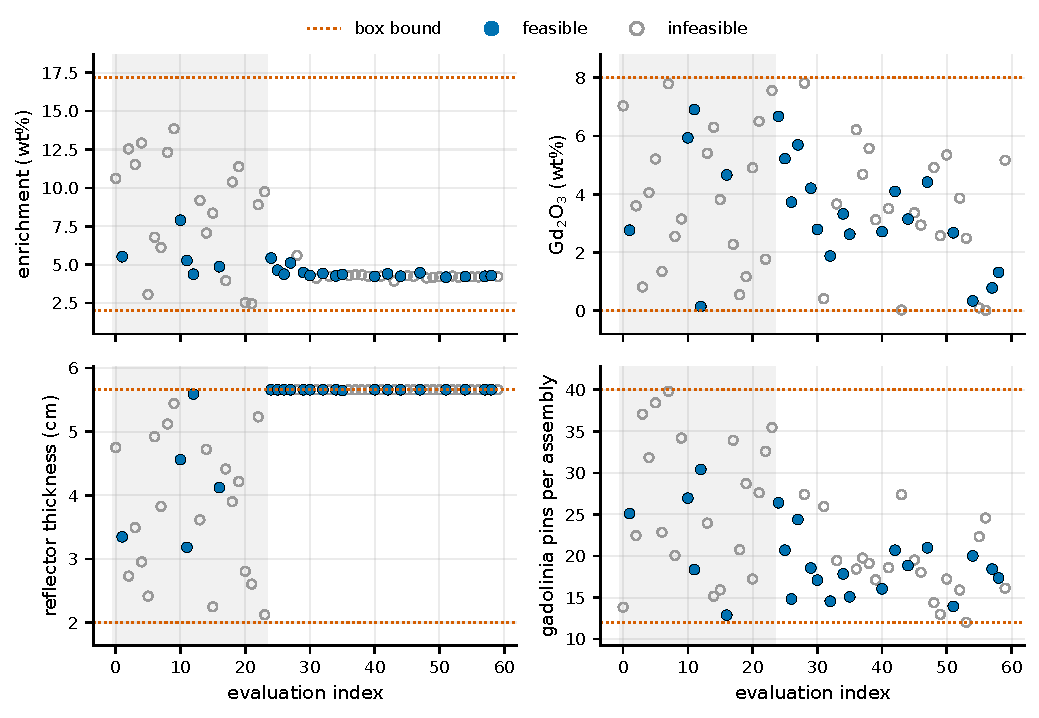
\includegraphics[width=\textwidth]{c9_design_space}
  \caption{Campaign 9: the four design variables along the evaluation order.}
  \label{fig:c9-design-space}
\end{figure}

Table~\ref{tab:c9-constraints} shows which constraints bind. The mission
constraint rejects the most designs, 22 of 60, followed by the reactivity
ceiling and the two control readings.

\begin{table}[htbp]
  \centering
  \caption{Campaign 9 archive, 60 evaluations: constraint satisfaction.}
  \label{tab:c9-constraints}
  \small
  \begin{tabular}{@{}lrrr@{}}
    \toprule
    Constraint & Satisfied & Minimum & Maximum \\
    \midrule
    $g_{k\min}$            & 50/60 & $-0.283$ & $+0.246$ \\
    $g_{k\max}$            & 46/60 & $-0.392$ & $+0.137$ \\
    $g_\mathrm{enr}$       & 60/60 & $-13.181$ & $-0.076$ \\
    $g_\mathrm{peak}$      & 55/60 & $-0.163$ & $+0.210$ \\
    $g_\mathrm{geom}$      & 60/60 & $-3.546$ & $-0.009$ \\
    $g_\mathrm{efpd}$      & 38/60 & $-5928.7$ & $+1826.0$ \\
    $g_\mathrm{ctrl,peak}$ & 47/60 & $-0.358$ & $+0.119$ \\
    $g_\mathrm{ctrl}$      & 47/60 & $-0.326$ & $+0.132$ \\
    \bottomrule
  \end{tabular}
\end{table}

Figure~\ref{fig:c9-pareto} places the archive in the objective plane. Open
circles are the 38 infeasible designs and filled circles the 22 feasible
ones, coloured by cycle length. The connected line is the five-member
front, labelled by archive index. The dashed and dotted horizontal lines
are the three-dimensional ceilings of C9-47, \SI{2897}{ppm} at
\SI{12.8}{MPa} and \SI{3244}{ppm} at \SI{15.5}{MPa}, drawn as reference
lines and not as constraints, and the shaded band at the top is the
\SI{6000}{ppm} clip. Three features stand out before the front itself:

\begin{enumerate}
  \item The feasible designs form a band. They span 1.490 to 1.647 in
        $F_{\Delta H}$ and 1406 to \SI{4371}{ppm} in $c_\mathrm{max}$, and
        the five front members occupy 0.055 of the first range. The boron
        objective separates these designs while the peaking objective
        barely does, which is what makes the front narrow.

  \item The designs at the clip are all infeasible. Eight designs sit on
        the \SI{6000}{ppm} plateau and every one is rejected on the
        reactivity or the control constraints, so the plateau never
        competes for a place on the front and the clip never influences the
        selection.

  \item Two feasible designs lie above both reference lines, C9-10 at
        \SI{4371}{ppm} and C9-12 at \SI{3003}{ppm}. Feasibility in the
        optimisation sense and operability are different properties, which
        is why the ceiling is drawn on the figure and not imposed as a
        constraint. C9-12 was scanned on its own lattice
        (Section~\ref{sec:res-c9-ceiling}) and fails its own ceiling by
        \SI{912}{ppm}, so the reference line understates its problem. No
        front member comes within \SI{980}{ppm} of the ceiling of C9-47.
\end{enumerate}

\begin{figure}[htbp]
  \centering
  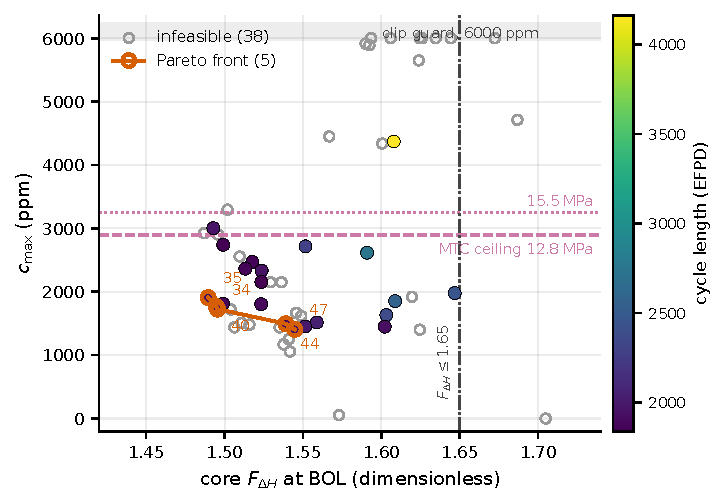
\includegraphics[width=0.86\textwidth]{c9_front}
  \caption{Campaign 9 archive in the reformulated objective plane.}
  \label{fig:c9-pareto}
\end{figure}

\subsection{Convergence and the reliability of the search}
\label{sec:res-c9-convergence}

The hypervolume history of the campaign is
\begin{equation*}
[\,879.1,\; 1244.5,\; 1291.4,\; 1291.6,\; 1318.5,\; 1318.5,\; 1318.5\,],
\end{equation*}
the first value being the design of experiments. Figure~\ref{fig:c9-hv}
draws the absolute hypervolume in the left panel and the gain of each
iteration against the \SI{1}{\%} threshold of the stopping rule in the
right. The first infill iteration is worth \SI{41.6}{\%}, the second
\SI{3.8}{\%} and the fourth \SI{2.1}{\%}, while iterations three, five and
six contribute \SI{0.02}{\%} or less. The gains are not monotone. A rule
that stopped at the first iteration below the threshold would have stopped
at iteration three and missed the \SI{2.1}{\%} of iteration four, which is
the error the three-iteration window of Section~\ref{sec:meth-loop} guards
against.

Under that window Campaign 9 is in the same position as Campaign 8
(Section~\ref{sec:res-c8-limits}). The gain fell below \SI{1}{\%} in the
last two iterations, so the third consecutive observation is missing and
the formal rule is not met. The hypervolume was nonetheless identical to
seven digits over the last three recorded values, and the cross-validation
and stability tests below find no sign that a further iteration would have
changed the front, so the front is reported as the best available and
effectively converged.

\begin{figure}[htbp]
  \centering
  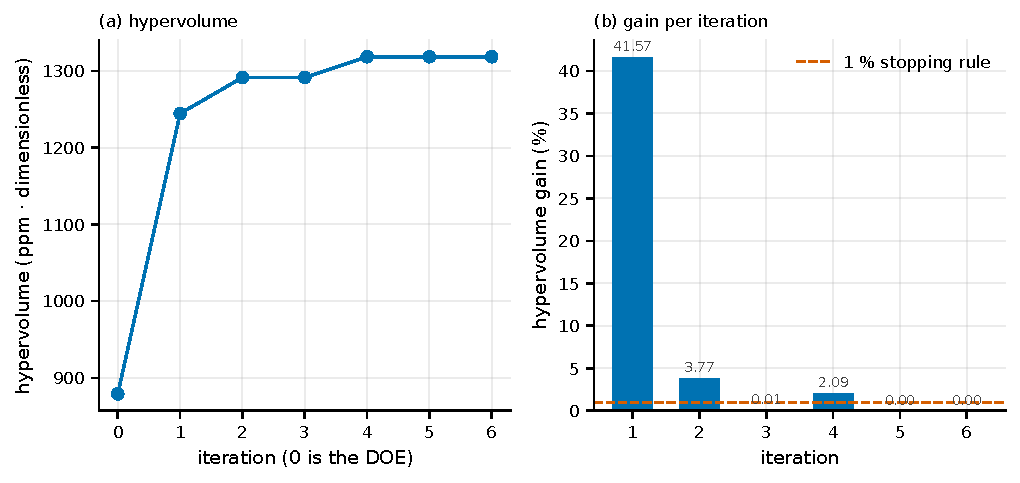
\includegraphics[width=\textwidth]{c9_hv}
  \caption{Campaign 9: hypervolume history and gain per iteration.}
  \label{fig:c9-hv}
\end{figure}

The infill is also visible in the objective. Figure~\ref{fig:c9-learning}
follows the boron requirement along the evaluation order, with the design
of experiments shaded, the best feasible value so far as a step line and
the phase means dashed. The mean falls from \SI{3977}{ppm} over the 24
designs of the Latin hypercube to \SI{1861}{ppm} over the 36 infill
designs, a factor of 2.1, and the best feasible value improves in seven
steps from 2615 to \SI{1406}{ppm}. Four of those steps fall in the first
six infill evaluations and the last at evaluation 47 of 60, consistent with
the flat tail of the hypervolume.

\begin{figure}[htbp]
  \centering
  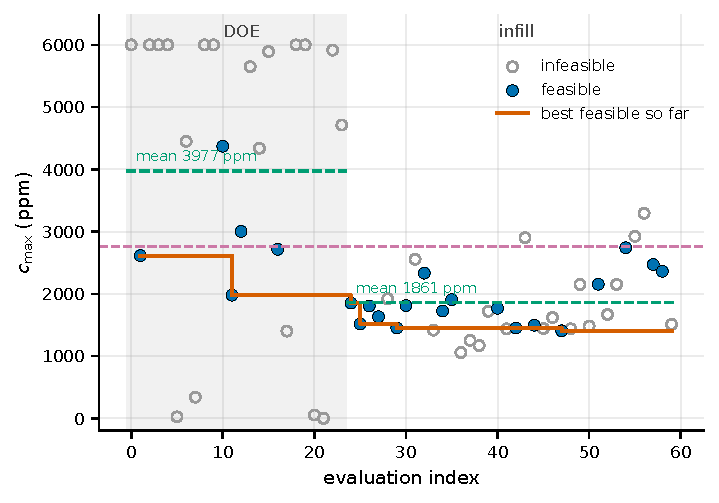
\includegraphics[width=0.86\textwidth]{c9_learning}
  \caption{Campaign 9: boron requirement along the evaluation order.}
  \label{fig:c9-learning}
\end{figure}

Two tests check whether that flat tail is convergence or exhaustion.

\paragraph{Surrogate cross-validation.}
Table~\ref{tab:c9-cv} gives the leave-one-out performance of the Gaussian
process on the full archive and on the feasible subset. The coverage is the
fraction of designs whose measured value falls inside the predicted
two-standard-deviation interval.

\begin{table}[htbp]
  \centering
  \caption{Campaign 9 surrogates: leave-one-out cross-validation.}
  \label{tab:c9-cv}
  \small
  \begin{tabular}{@{}llrrr@{}}
    \toprule
    Objective & Set & $R^2$ & RMSE & Coverage \\
    \midrule
    $F_{\Delta H}$    & all 60      & $+0.862$ & 0.026 & 0.92 \\
    $F_{\Delta H}$    & feasible 22 & $+0.276$ & 0.039 & 0.82 \\
    $c_\mathrm{max}$  & all 60      & $+0.964$ & \SI{342}{ppm} & 0.87 \\
    $c_\mathrm{max}$  & feasible 22 & $+0.387$ & \SI{530}{ppm} & 0.86 \\
    \bottomrule
  \end{tabular}
\end{table}

The coefficient of determination drops on the feasible subset for two
reasons, and the drop should not be quoted without them.

\begin{enumerate}
  \item The coefficient measures accuracy relative to the spread of the
        data. The full archive spans $c_\mathrm{max}$ from \SI{0}{ppm} to
        the \SI{6000}{ppm} clip, while the feasible subset spans 1406 to
        \SI{3003}{ppm} once its single long-cycle outlier, C9-10, is set
        aside. The denominator shrinks by about an order of magnitude and
        the numerator does not.

  \item The feasible fit has 21 training points for a four-dimensional
        kernel with automatic relevance determination, clustered inside a
        \SI{0.3}{wt\%} enrichment band, which leaves the kernel little
        leverage to identify its length scales.
\end{enumerate}

For the acquisition the coverage matters more, and it holds at 0.82 and
0.86 on the feasible subset, close to the nominal 0.954. The Campaign 8
surrogate reached 0.89 on its feasible subset (Table~\ref{tab:c8-cv-loo}),
so the Campaign 9 surrogate is somewhat less well calibrated on the
feasible designs, but not to the point of steering the acquisition. Inside
the converged region the design-to-design variation of the objectives is
comparable to the measurement noise, so the surrogate cannot resolve which
candidate is better and the acquisition cannot propose a new one. The low
feasible-subset $R^2$ and the flat hypervolume record the same state.

\paragraph{Front stability.}
Each archived objective was perturbed by a noise of 0.010 in $F_{\Delta H}$
and \SI{10}{ppm} in $c_\mathrm{max}$, and the feasible non-dominated set
was recomputed 2000 times. Table~\ref{tab:c9-stability} gives the frequency
with which each design appears on the front, omitting designs below
\SI{5}{\%}. The peaking noise was assumed at the time and is compared with
the measured value in Section~\ref{sec:res-c9-peaking}.

\begin{table}[htbp]
  \centering
  \caption{Campaign 9 archive, 2000 noise perturbations: Pareto membership frequency.}
  \label{tab:c9-stability}
  \small
  \begin{tabular}{@{}lrc@{}}
    \toprule
    Design & Frequency & On the nominal front \\
    \midrule
    C9-47 & 1.00 & yes \\
    C9-34 & 1.00 & yes \\
    C9-44 & 0.59 & yes \\
    C9-40 & 0.54 & yes \\
    C9-35 & 0.45 & yes \\
    C9-29 & 0.31 & no \\
    C9-30 & 0.24 & no \\
    C9-12 & 0.21 & no \\
    C9-54 & 0.10 & no \\
    \bottomrule
  \end{tabular}
\end{table}

Figure~\ref{fig:c9-front-stability} draws the same frequencies. Coloured
bars are members of the nominal front, grey bars are designs that join it
only under the noise, and the dotted line is a simple majority. The front
separates into three groups. C9-47 and C9-34 are on it in every resample,
a robust core of two designs. C9-44, C9-40 and C9-35 sit around the
majority line, so their membership is decided by the noise, and C9-35
falls short of a majority. C9-29 and C9-30 are excluded from the nominal
front by margins smaller than the noise and join it in about a quarter of
the resamples, so the candidate set carried forward from this campaign is
the seven designs of these three groups, and not only the five of
Table~\ref{tab:c9-front}. C9-12 also joins the front in a fifth of the
resamples, but it fails the ceiling of its own lattice
(Section~\ref{sec:res-c9-ceiling}).

\begin{figure}[htbp]
  \centering
  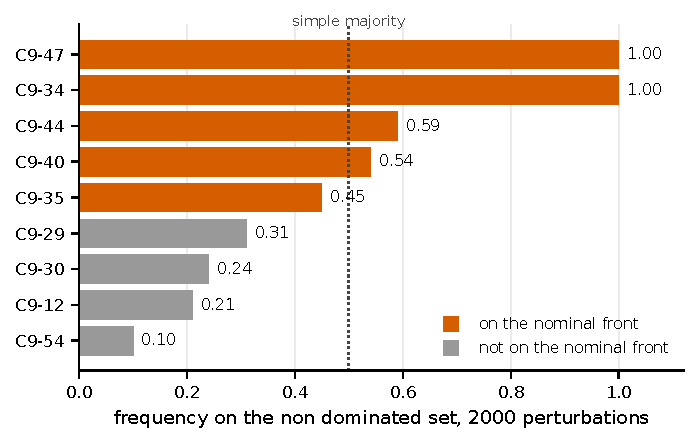
\includegraphics[width=0.80\textwidth]{c9_front_stability}
  \caption{Campaign 9 archive, 2000 noise perturbations: Pareto membership frequency.}
  \label{fig:c9-front-stability}
\end{figure}

The hypervolume of the perturbed fronts exceeds that of the nominal front
by a factor of $1.028 \pm 0.024$. The front is a set of extremes: a design
pushed by the noise toward lower values of both objectives joins it, while
a design pushed the other way is replaced. The selection is one-sided, as in
the winner's curse, and the \SI{2.8}{\%} excess measures how much of the
apparent quality of a front comes from selection.

\subsection{Scoring under the original formulation}
\label{sec:res-c9-discarded}

The Campaign 9 archive can be scored under the Campaign 8 objectives,
maximum cycle length and minimum peaking, with the Campaign 8 constraint
set. Under those rules 35 of the 60 designs are feasible and seven are
non-dominated, and only one of the seven, C9-35, is also on the Campaign 9
front. Table~\ref{tab:c9-depth} gives the non-domination depth of each
Campaign 9 front member under the Campaign 8 objectives, over those 35
designs. A depth of one means the design would have been selected, and a
higher depth counts the fronts that would have to be removed first.

\begin{table}[htbp]
  \centering
  \caption{Campaign 9 front scored under the Campaign 8 objectives: non-domination depth.}
  \label{tab:c9-depth}
  \small
  \begin{tabular}{@{}lcr@{}}
    \toprule
    Design & Depth under the C8 objectives & $c_\mathrm{max}$ [ppm] \\
    \midrule
    C9-47 & 3 & 1406 \\
    C9-44 & 4 & 1496 \\
    C9-34 & 3 & 1725 \\
    C9-40 & 2 & 1768 \\
    C9-35 & 1 & 1908 \\
    \bottomrule
  \end{tabular}
\end{table}

Four of the five front members, including C9-47, would have lain two to
four fronts deep and would never have entered the Campaign 8 candidate
set. The objective set decided the Campaign 8 outcome, and the search found
what that set asked for.

Figure~\ref{fig:c9-two-formulations} shows the same fact in the Campaign 8
objective plane. Crosses are designs the Campaign 8 constraint set rejects,
grey circles the 35 it accepts and open squares the seven its objectives
select, circles outlined in colour are the Campaign 9 front coloured by
boron requirement, and the dashed vertical line is the mission floor. The
Campaign 9 front members sit in the interior of the plane, short of the
cycle-length frontier, where a cycle-length objective does not look. The
inset enlarges their cluster. They occupy \SI{106}{d} of cycle length, 1841
to \SI{1947}{d}, which the Campaign 8 objectives read as the worst corner of
the feasible set on the cycle-length axis, while the peaking objective
barely separates them. Only C9-35 is picked up by both formulations, and it
has the highest boron requirement of the five, \SI{1908}{ppm}.

\begin{figure}[htbp]
  \centering
  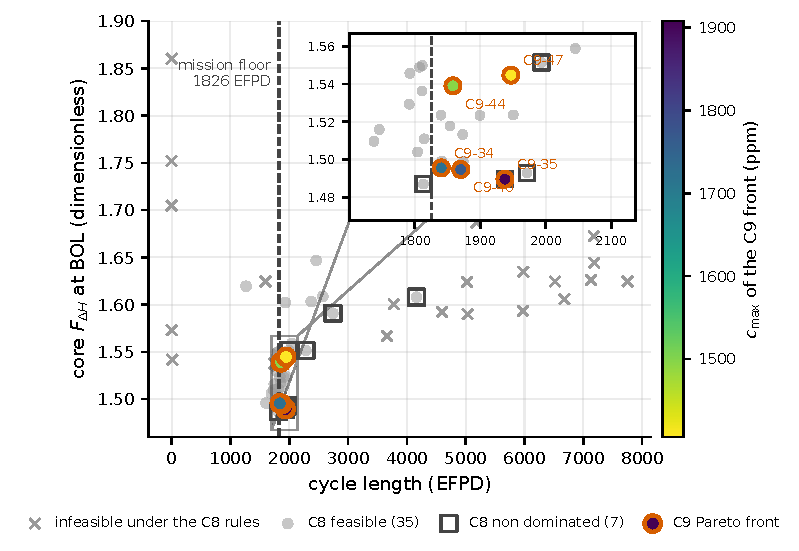
\includegraphics[width=0.92\textwidth]{c9_two_formulations}
  \caption{Campaign 9 archive in the Campaign 8 objective plane.}
  \label{fig:c9-two-formulations}
\end{figure}

The seven designs the Campaign 8 objectives would select span 1813 to
\SI{4163}{d} and need 1452 to \SI{4371}{ppm}. Three of them, C9-55 at
\SI{2923}{ppm}, C9-12 at \SI{3003}{ppm} and C9-10 at \SI{4371}{ppm},
exceed the ceiling of C9-47, \SI{2897}{ppm}, and C9-12 also fails the
ceiling of its own lattice by \SI{912}{ppm}. An objective set built on cycle
length
would again have placed a substantial part of its selection outside the
operable region, the Campaign 8 outcome reproduced on a different archive.

\subsection{Comparison with the Campaign 8 candidates}
\label{sec:res-c9-compare}

The two campaigns do not converge on the same designs. C8-47 lies at a
normalised design-space distance of 0.401 from the nearest Campaign 9 front
member, and C8-13 at 0.722, both far outside the minimum infill separation
of 0.14. Much of that distance is the reflector, 4.29 and \SI{3.15}{cm}
against 5.65 to \SI{5.66}{cm} on the Campaign 9 front. Inside the Campaign 8
box the reflector is worth only about \SI{52}{pcm} per centimetre through
the target (Section~\ref{sec:res-c8-refl}). At the mission floor, where
every design sits near the minimum reactivity the cycle needs, that small
gain lowers the enrichment required, and the enrichment drives the boron
demand, which is consistent with a boron objective pushing every front
member to the reflector bound.

Placed on the Campaign 9 objectives, both Campaign 8 designs that the
retrospective of Section~\ref{sec:res-c8-retro} selected at the same floor
are dominated. Both have a negative hump, so their concentration at the
operating maximum is the beginning-of-life value.

\begin{enumerate}
  \item C8-47, at $F_{\Delta H} = 1.510$, \SI{2327}{ppm} and 1941\,EFPD, is
        dominated by C9-35, C9-40 and C9-34, which need 419 to
        \SI{602}{ppm} less boron at a peaking factor lower by 0.014 to
        0.020. The peaking differences are within about one and a half seed
        standard deviations of Campaign 8, so the dominance rests on the
        boron demand.

  \item C8-13, at $F_{\Delta H} = 1.632$, \SI{1697}{ppm} and 2383\,EFPD, is
        dominated by C9-47 and C9-44 on both objectives, by 291 and
        \SI{201}{ppm} and by 0.087 and 0.093 in peaking.
\end{enumerate}

C8-53 needs \SI{1312}{ppm}, less than any member of the Campaign 9 front,
but its cycle of 1142\,EFPD does not meet the floor. The comparison is
indicative, because the Campaign 8 concentrations come from the
post-analysis, a measured root for C8-47 and a linear estimate for C8-13,
while the Campaign 9 concentrations come from the probe solves of the
evaluator.

\subsection{Gadolinia, boron demand and the mid-cycle hump}
\label{sec:res-c9-gd}

The mechanism behind the front shows in the 16 feasible designs within
\SI{0.35}{wt\%} of the mean front enrichment of \SI{4.31}{wt\%}. Over that
band the gadolinia loading spans 0.14 to \SI{5.22}{wt\%} and the boron
requirement 1406 to \SI{3003}{ppm}, at nearly constant enrichment and with
the same reflector on all but one design. Table~\ref{tab:c9-gd-corr} gives
the rank correlations. The Spearman coefficients use average ranks, which
is necessary because the hump is set to zero below its \SI{400}{pcm} noise
floor and nine designs are tied there, and the inventory is the product of
the gadolinia weight fraction and the number of poisoned pins.

\begin{table}[htbp]
  \centering
  \caption{Campaign 9 feasible designs at $4.31 \pm \SI{0.35}{wt\%}$: rank correlations with the gadolinia loading.}
  \label{tab:c9-gd-corr}
  \small
  \begin{tabular}{@{}llrrr@{}}
    \toprule
    Predictor & Response & Spearman $\rho_S$ & $p$ & Kendall $\tau_b$ \\
    \midrule
    Gd weight fraction & $c_\mathrm{max}$ & $-0.932$ & $1.5\times10^{-7}$ & $-0.817$ \\
    Gd inventory       & $c_\mathrm{max}$ & $-0.953$ & $1.2\times10^{-8}$ & --- \\
    Gd weight fraction & hump             & $-0.723$ & $0.002$ & $-0.598$ \\
    Gd inventory       & hump             & $-0.684$ & $0.003$ & --- \\
    \bottomrule
  \end{tabular}
\end{table}

At fixed enrichment the boron requirement falls by \SI{1597}{ppm} as the
gadolinia rises. The cycle-length formulation could not reward that
relation, because gadolinia entered it only as a cost against cycle length.

\paragraph{The two predictors.}
The weight fraction and the inventory give $-0.932$ and $-0.953$, and the
archive does not show that the inventory is the better variable. Over the
band the two predictors have a rank correlation of $+0.988$ with each other,
because the weight fraction varies by a factor of 37 while the pin count
varies by a factor of 2.7. A difference of 0.021 between two predictors
that order the designs almost identically cannot be resolved on 16 samples,
and the same applies to the hump, where the weight fraction leads by 0.039.

\paragraph{Matched comparisons.}
Comparing designs matched in one variable and differing in the other
removes the confounding. Five pairs in the band share a gadolinia weight
fraction to within \SI{0.25}{wt\%} and differ in pin count. In four of the
five the design with more poisoned pins needs less boron, by 229 to
\SI{387}{ppm}, but three of those four involve the same 12-pin design, so
they amount to two independent observations. The fifth pair reverses, and
both its members carry almost no gadolinia, 0.14 and \SI{0.33}{wt\%}, so the
relation does not hold at negligible loading.

The hump allows a sharper test. Two pairs in the band are matched in
inventory to within \SI{7}{\%} and differ in concentration, and
Table~\ref{tab:c9-pairs} lists them. Both pairs carry the same reflector of
\SI{5.66}{cm}.

\begin{table}[htbp]
  \centering
  \caption{Campaign 9 feasible designs matched in gadolinia inventory: concentration against hump.}
  \label{tab:c9-pairs}
  \small
  \begin{tabular}{@{}lrrrrrrr@{}}
    \toprule
    Design & $e$ & Gd$_2$O$_3$ & pins & inventory & $c_\mathrm{BOL}$ &
    $c_\mathrm{max}$ & hump \\
     & wt\% & wt\% & & wt\%\,pins & ppm & ppm & pcm \\
    \midrule
    C9-26 & 4.38 & 3.73 & 16 & 59.7 & 1805 & 1805 & 0 \\
    C9-44 & 4.24 & 3.15 & 20 & 62.9 & 1334 & 1496 & $+1093$ \\
    \addlinespace
    C9-32 & 4.42 & 1.88 & 16 & 30.0 & 2121 & 2333 & $+1349$ \\
    C9-51 & 4.18 & 2.68 & 12 & 32.1 & 2154 & 2154 & 0 \\
    \bottomrule
  \end{tabular}
\end{table}

Both pairs point the same way. At matched inventory the design with the
higher concentration in each poisoned pin shows no resolved hump, while its
partner shows a hump of 1093 and \SI{1349}{pcm}. The enrichment differs by
0.14 and \SI{0.24}{wt\%} within the pairs, and in both cases the difference
acts against the observed effect, since the design without the hump carries
the higher enrichment, so the effect is if anything understated.

The second pair reverses the ranking. At beginning of life C9-32 needs less
boron, 2121 against \SI{2154}{ppm}. At the operating maximum C9-51 needs
less, 2154 against \SI{2333}{ppm}. At matched inventory and identical
reflector, which of the two needs less boron depends on the state at which
the question is asked, which is the clearest single demonstration in this
work that the objective has to be defined at the operating maximum.

\paragraph{Mechanism.}
The hump of Equation~\eqref{eq:c7-hump} is the difference between the
reactivity at the mid-cycle maximum and at beginning of life, and the
gadolinium suppresses both terms. It is governed by a race between
gadolinium burnout, which raises the multiplication factor, and fuel
depletion with fission-product build-up, which lowers it.

A dilute gadolinia pin is nearly transparent to thermal neutrons through
its volume, so it burns out quickly and uniformly, within the first few
\si{MWd\per kg} of burnup and before appreciable fuel depletion. Almost the
whole poison worth returns as a rise above the beginning-of-life point, and
the hump is large. A concentrated pin shields its own interior and burns
inward from the surface over many \si{MWd\per kg}, by which time fuel
depletion has removed a comparable amount of reactivity, so the two effects
cancel and the multiplication factor does not climb above its initial
value.

The grouped statistic supports the same reading. Of the 16 designs in the
band, the seven with a resolved hump carry a mean gadolinia weight fraction
of \SI{1.67}{wt\%}, against \SI{3.52}{wt\%} for the nine without, and a
one-sided Mann-Whitney test gives $U = 10$ and $p = 0.012$. That test is
used in preference to the rank correlation because it is insensitive to the
nine ties at the noise floor.

Figure~\ref{fig:c9-gd-mechanism} shows the mechanism. The left panel draws
the boron requirement of the 22 feasible designs against gadolinia content,
coloured by enrichment, where the two effects are mixed. The right panel
draws the 16 designs of the band, with the beginning-of-life concentration
as an open circle, the objective as a filled circle, the bar between them
equal to the hump expressed in ppm, a least-squares fit to $c_\mathrm{max}$
dashed and the two boron ceilings as horizontal lines.

\begin{figure}[htbp]
  \centering
  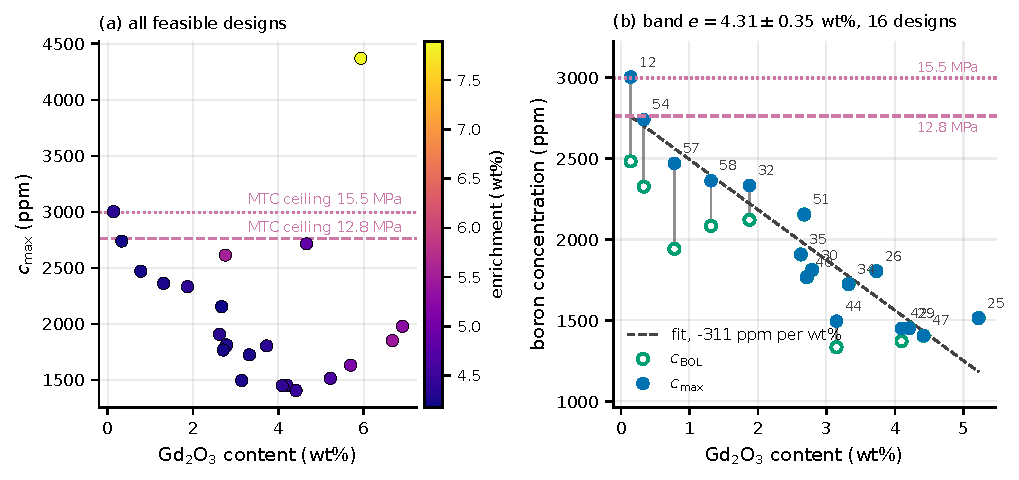
\includegraphics[width=\textwidth]{c9_gd_trade}
  \caption{Campaign 9 feasible designs: boron requirement against gadolinia content.}
  \label{fig:c9-gd-mechanism}
\end{figure}

Read across the band, three things happen as the gadolinia rises. The
beginning-of-life concentration falls, because the poison holds down
reactivity that boron would otherwise have to hold. The bars shorten and
then vanish, because the hump disappears above roughly \SI{2.5}{wt\%}. And
the two quantities converge, so that above that loading the objective and
its beginning-of-life value are the same number. One design of the band
sits above the ceiling of C9-47, C9-12 at \SI{3003}{ppm}, the most dilute
of the sixteen at \SI{0.14}{wt\%}. Its beginning-of-life requirement is
\SI{2482}{ppm}, below that line, so the hump alone carries it above.

The lattice scan of Section~\ref{sec:res-c9-ceiling} makes the case stronger
than the reference line allows. The ceiling of C9-12 is \SI{2091}{ppm}, not
\SI{2897}{ppm}, because the same dilution that raises its demand also lowers
what it can tolerate. Judged against its own lattice the design fails by
\SI{912}{ppm} instead of \SI{106}{ppm}, and even its beginning-of-life
requirement is \SI{391}{ppm} too high. An objective evaluated at beginning
of life would therefore also have rejected this design, but only once its
own ceiling was known.

Figure~\ref{fig:c9-hump} isolates the hump over the whole feasible set. The
left panel draws it against gadolinia content, with filled circles for the
designs inside the band and the \SI{400}{pcm} noise floor marked. The hump
reaches \SI{3430}{pcm} at negligible loading and falls below the noise floor
above \SI{2.5}{wt\%}. Only two feasible designs above that loading retain a
resolved hump, of \SI{1093}{pcm} at \SI{3.15}{wt\%} and \SI{512}{pcm} at
\SI{4.10}{wt\%}, and both carry their gadolinia on 20 pins instead of 16,
which is the matched comparison of Table~\ref{tab:c9-pairs} seen from the
other side.

The right panel draws the penalty the hump carries into the objective
against the hump itself, and confirms that it enters as
Equation~\eqref{eq:c9-cmax} prescribes. It is proportional to the hump with
a slope of \SI{0.153}{ppm} per pcm, an implied boron worth of
\SI{6.5}{pcm} per ppm, against \SI{6.35}{pcm} per ppm measured as the mean
over the eight designs that carry a hump. The agreement is a consistency
check on the implementation, and it is reported because it is the only
direct verification that the hump term and the measured worth are combined
correctly.

\begin{figure}[htbp]
  \centering
  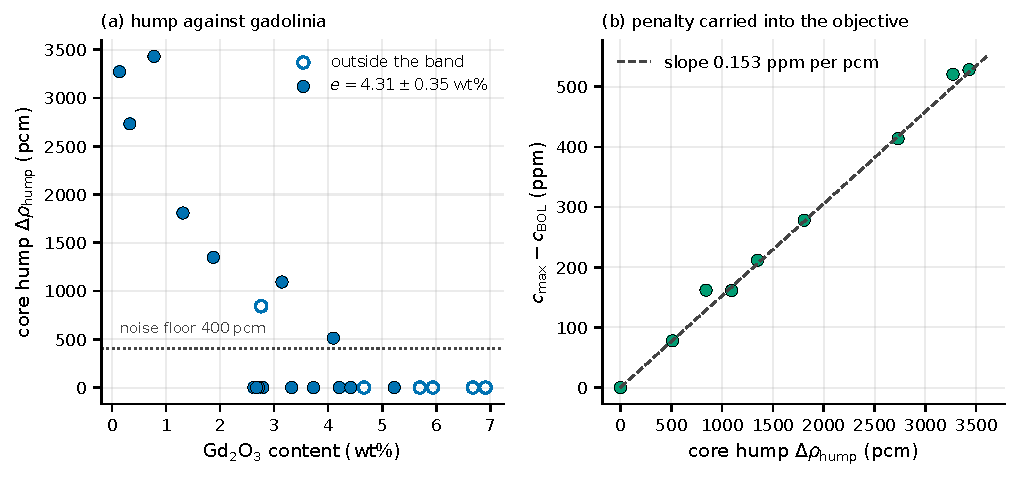
\includegraphics[width=\textwidth]{c9_hump}
  \caption{Campaign 9 feasible designs: mid-cycle hump and the boron penalty it carries.}
  \label{fig:c9-hump}
\end{figure}

The mechanism is inferred from two matched pairs and a grouped test. A
designed set of four or five assemblies at fixed gadolinia inventory
spanning 12 to 40 poisoned pins, one depletion each, about one hour of
machine time, would settle it, and the multiplication-factor histories of a
humped and an unhumped front design, already written by
\texttt{validate\_ktarget\_burnup.py}, would show the burnout timescale
directly at no additional cost.

\subsection{The peaking objective under fidelity and dimensionality}
\label{sec:res-c9-peaking}

The five front designs were re-solved with all rods out at
\num{150000} particles and 200 batches with 80 inactive, two seeds, on the
two-dimensional core and on the three-dimensional core model of
Section~\ref{sec:res-c8-3d}. Three quantities can be separated from those
solves: the seed reproducibility, the effect of raising the transport
statistics, and the effect of the third dimension.

\paragraph{Seed reproducibility.}
The ten pairs of seeds differ by 0.0069 on average in $F_{\Delta H}$. For
two independent samples of a normal variable the expected absolute
difference is $2\sigma/\sqrt{\pi}$, so the pooled single-solve standard
deviation is

\begin{equation}
\sigma_F = \frac{0.0069\,\sqrt{\pi}}{2} = 0.0061
\label{eq:c9-sigmaF}
\end{equation}

\noindent where $\sigma_F$ is the standard deviation of a single solve of
$F_{\Delta H}$ at these statistics, dimensionless. It gives 0.0043 on a
two-seed mean and 0.0061 on the difference between two such means. The
Campaign 8 post-analysis measured 0.011 at the same statistics with all
rods out, pooled over fourteen pairs (Section~\ref{sec:res-c8-sigma}), so
the Campaign 9 front designs are somewhat less noisy. Scaled to the archive fidelity with the
same factor used there, the Campaign 9 value is about 0.008, so the 0.010
assumed in the stability analysis of Section~\ref{sec:res-c9-convergence}
is conservative for these designs by about a quarter.

\paragraph{Fidelity.}
Table~\ref{tab:c9-peaking} compares the archived campaign value, a single
solve at \num{100000} particles and 170 batches with 60 inactive, against
the two-dimensional confirmation at the higher statistics. The shifts are
$-0.009$, $-0.014$, $+0.001$, $-0.025$ and $-0.018$, a mean of $-0.013$ with
a standard error of 0.004. The direction follows from the estimator: the
hot channel factor is a maximum over mesh bins, the maximum of a set of
noisy bins is biased upward (Section~\ref{sec:bg-mc}), and raising the
statistics lowers the estimate. The shift is about a quarter of the width
of the whole front on that objective.

\paragraph{Dimensionality.}
The three-dimensional shift is not a constant. Two designs move by $-0.026$
and $-0.040$, 4.3 and 6.6 times the 0.0061 uncertainty of the comparison,
while the other three move by $+0.005$, $+0.006$ and $-0.001$, none of which
is resolved. The mean ratio $F^\mathrm{3D}/F^\mathrm{2D}$ is 0.992 with a
standard deviation of 0.014 over the five designs. In the table the
confirmation columns are means of two seeds, and the uncertainty on a
difference between two confirmation columns is 0.006,
Equation~\eqref{eq:c9-sigmaF}.

\begin{table}[htbp]
  \centering
  \caption{Campaign 9 front, all rods out: hot channel factor as archived, confirmed in 2D and in the 3D core model.}
  \label{tab:c9-peaking}
  \small
  \begin{tabular}{@{}lrrrrrr@{}}
    \toprule
    Design & archive & 2D conf. & 3D conf. & fidelity & 3D shift &
    3D shift \\
     & $F$ & $F$ & $F$ & shift & & in $\sigma$ \\
    \midrule
    C9-35 & 1.490 & 1.481 & 1.487 & $-0.009$ & $+0.006$ & 1.0 \\
    C9-34 & 1.496 & 1.482 & 1.487 & $-0.014$ & $+0.005$ & 0.8 \\
    C9-40 & 1.495 & 1.496 & 1.456 & $+0.001$ & $-0.040$ & 6.6 \\
    C9-44 & 1.539 & 1.514 & 1.513 & $-0.025$ & $-0.001$ & 0.2 \\
    C9-47 & 1.545 & 1.527 & 1.501 & $-0.018$ & $-0.026$ & 4.3 \\
    \bottomrule
  \end{tabular}
\end{table}

\paragraph{Consequence for the front.}
With the two-dimensional confirmation values the non-dominated set of these
five designs in $(F_{\Delta H}, c_\mathrm{max})$ is C9-34, C9-35, C9-44 and
C9-47, since C9-34 then dominates C9-40. With the three-dimensional values
it becomes C9-34, C9-40 and C9-47. The three changes are of unequal
standing.

\begin{enumerate}
  \item C9-40 enters the front because its hot channel factor falls by
        0.040, a 6.6$\sigma$ effect. This change is measured.

  \item C9-44 leaves the front because C9-47 improves by 0.026 while C9-44
        does not move, so in three dimensions C9-47 has both the lower
        peaking, 1.501 against 1.513, and the lower boron requirement, 1406
        against \SI{1496}{ppm}. This change is measured.

  \item C9-35 leaves the front because it becomes dominated. Against C9-34
        the dominance is not resolved, because both designs reach a peaking
        of 1.487 and the boron requirement alone separates them, 1725
        against \SI{1908}{ppm}. Against C9-40 it is resolved, with a peaking
        of 1.456 against 1.487 and a boron requirement of 1768 against
        \SI{1908}{ppm}, so this change stands or falls with the shift of
        C9-40 in the first item.
\end{enumerate}

A design-dependent shift of this size is the case in which a
three-dimensional objective reorders a front instead of translating it, so
a calibrated correction applied to the two-dimensional value would not
recover the same answer, as the zoned proxy gap of
Section~\ref{sec:res-proxy-gap-zoned} found for the assembly value.

One caution applies to this five-design comparison. C9-40, the design
that drives the front change, has a two-seed spread of 0.017 in the
two-dimensional solve against 0.001 to 0.004 for the other four, so its
own convergence is the least well established of the set.

\paragraph{The comparison over the whole archive.}
The comparison with all rods out was extended to all sixty designs, one
solve per design in each model with two seeds. The three-dimensional hot
channel factor is lower than the two-dimensional one for almost every
design, by 0.023 on average with a standard deviation of 0.017, a ratio of
0.9851 with a relative spread of \SI{1.10}{\%}. The correction is therefore
not a constant, and the rank correlation between the two orderings is 0.941,
with a largest rank shift of 14 places out of 60.

Recomputed over the 22 feasible designs, the non-dominated set is C9-34,
C9-35, C9-44, C9-47 and C9-58 with the two-dimensional factor, and C9-12,
C9-34, C9-40 and C9-47 with the three-dimensional one. Three observations
bound what that change means:

\begin{enumerate}
  \item C9-47 is on both fronts. It is selected whichever factor is used, so
        the reordering does not reach the design the campaign selects.

  \item The newcomer is inoperable. C9-12 fails the ceiling of its own
        lattice by \SI{912}{ppm} (Section~\ref{sec:res-c9-ceiling}), so it
        cannot be a candidate whatever its peaking.

  \item Part of the change comes from fidelity. The two-dimensional values of
        this comparison are solved at \num{150000} particles over 200
        batches, while the archive values are solved at \num{100000} over
        170. Over the 41 designs common to both, the higher-fidelity value is
        lower by 0.016 on average with a standard deviation of 0.017,
        reaching 0.068 on C9-42 and 0.037 on C9-58. A hot channel factor is
        a maximum over channels, and a maximum over noisier estimates is
        biased upward (Section~\ref{sec:bg-mc}), so the campaign-fidelity
        value reads high. C9-58 enters the two-dimensional front of this
        comparison largely through that shift.
\end{enumerate}

The quantities that matter are of the same size. The peaking spread across
the whole front is 0.055, the dimensional shift 0.023, the fidelity shift
0.016, and the leave-one-out error of the surrogate on the feasible subset
0.039 (Table~\ref{tab:c9-cv}). A campaign that optimised this objective more
finely could not resolve differences of this size, which argues against a
further campaign on the peaking objective more strongly than the front
change does on its own. The three-dimensional peaking of C9-47 is therefore
reported as a verified value, 1.501 against 1.527 in two dimensions, both
well inside the 1.65 constraint.

\subsection{The boron ceiling of each candidate lattice}
\label{sec:res-c9-ceiling}

Campaign 8 measured one moderator temperature coefficient ceiling, on the
lattice of C8-47, and Campaign 9 inherited it as a single reference line.
That inheritance does not hold. The coefficient responds to a change in
moderator density, and the response depends on the absorber loading of the
lattice, which is a design variable. Eight lattices were therefore scanned
on the three-dimensional core model at \SI{12.8}{MPa}: every candidate on either peaking
front of Section~\ref{sec:res-c9-peaking}, and C9-57 as a diagnostic design.

\paragraph{Method.}
Each scan solves the core at two moderator temperatures and four boron
concentrations, two seeds each, sixteen solves per design. The moderator
states are the following, with densities from the IAPWS-IF97 formulation
and saturation at \SI{602.8}{K} and \SI{617.9}{K}:

\begin{itemize}
  \item \SI{547}{K} and \SI{567}{K} at \SI{12.8}{MPa}, with densities of
        \SI{0.77109}{g/cm^3} and \SI{0.73403}{g/cm^3} and a subcooling of
        \SI{55.8}{K} and \SI{35.8}{K}.

  \item \SI{570}{K} and \SI{590}{K} at \SI{15.5}{MPa}, used for C9-47 only.
\end{itemize}

The window at \SI{12.8}{MPa} is the one of Section~\ref{sec:res-c8-swing},
so the Campaign 8 and Campaign 9 ceilings can be compared directly.

The ceiling is the concentration at which the coefficient changes sign. It
is obtained by a weighted straight-line fit of the coefficient against
concentration over the three points nearest the sign change. Its
uncertainty is propagated from the fit covariance and inflated by
$\sqrt{\chi^2/\nu}$ where that exceeds unity. Three of the eight scans have
$\chi^2/\nu$ above two, the signature of a mild curvature of the coefficient
in boron, and the inflation keeps their error bars honest.

\paragraph{The ceiling of C9-47.}
The ceiling of C9-47 was measured in two and in three dimensions at both
pressures:

\begin{itemize}
  \item \SI{2415}{ppm} at \SI{12.8}{MPa} in two dimensions.

  \item \SI{2897}{ppm} at \SI{12.8}{MPa} in three dimensions, with a refit
        uncertainty of \SI{99}{ppm}.

  \item \SI{2653}{ppm} at \SI{15.5}{MPa} in two dimensions.

  \item \SI{3244}{ppm} at \SI{15.5}{MPa} in three dimensions.
\end{itemize}

The move from two to three dimensions raises the ceiling by \SI{482}{ppm} at
\SI{12.8}{MPa} and by \SI{591}{ppm} at \SI{15.5}{MPa}. On C8-47 the same
shift was \SI{508}{ppm}, so the axial leakage feedback of
Section~\ref{sec:res-c8-3d} reproduces on an independent lattice. A ceiling
computed in two dimensions is conservative by roughly that amount, which is
useful because the two-dimensional scan costs a quarter of the
three-dimensional one.

\paragraph{The eight lattices.}
Table~\ref{tab:c9-ceilings} gives the eight lattices, and
Figure~\ref{fig:c9-ceiling} draws them against the gadolinia inventory, the
weight fraction multiplied by the number of gadolinia pins, which is
proportional to the mass of gadolinia per assembly. In the left panel the
measured ceiling and the boron demand of each design are joined by a
vertical bar on a logarithmic inventory axis, with the logarithmic fit
dashed. The right panel draws the operating margin, the ceiling minus the
demand, with the two designs that fail their own ceiling in a separate
colour. The error bars are the refit uncertainty.

\begin{table}[htbp]
  \centering
  \caption{Campaign 9 candidate lattices at \SI{12.8}{MPa} in three dimensions: boron ceiling, demand and margin.}
  \label{tab:c9-ceilings}
  \small
  \begin{tabular}{@{}lrrrrrr@{}}
    \toprule
    Design & Gd (wt\%) & pins & inventory & ceiling (ppm) & demand (ppm) & margin (ppm) \\
    \midrule
    C9-12 & 0.14 & 32 & 4.5 & $2091 \pm 69$ & 3003 & $-912$ \\
    C9-57 & 0.78 & 20 & 15.6 & $2278 \pm 173$ & 2470 & $-193$ \\
    C9-58 & 1.31 & 16 & 21.0 & $2483 \pm 53$ & 2363 & $+120$ \\
    C9-35 & 2.63 & 16 & 42.0 & $2617 \pm 69$ & 1908 & $+710$ \\
    C9-40 & 2.71 & 16 & 43.4 & $2651 \pm 240$ & 1768 & $+883$ \\
    C9-34 & 3.32 & 16 & 53.2 & $2752 \pm 97$ & 1725 & $+1027$ \\
    C9-44 & 3.15 & 20 & 62.9 & $2858 \pm 109$ & 1496 & $+1362$ \\
    C9-47 & 4.42 & 20 & 88.4 & $2897 \pm 99$ & 1406 & $+1491$ \\
    \bottomrule
  \end{tabular}
\end{table}

\begin{figure}[htbp]
  \centering
  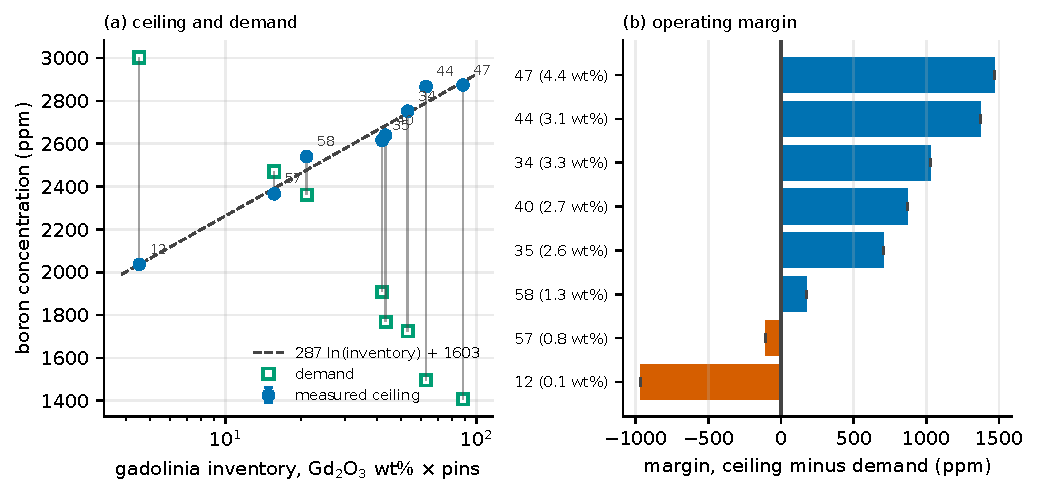
\includegraphics[width=\textwidth]{c9_ceiling_inventory}
  \caption{Campaign 9, eight lattices at \SI{12.8}{MPa}: boron ceiling and demand against gadolinia inventory.}
  \label{fig:c9-ceiling}
\end{figure}

\paragraph{The second pressure.}
Five of the eight lattices were scanned again at \SI{15.5}{MPa}, and
Table~\ref{tab:c9-ceilings-p155} reports that set.
Figure~\ref{fig:c9-ceiling-2p} draws both pressures against the two
measures of gadolinia loading and the shift between them. The eight
lattices span inventories from 4.5 for C9-12 to 88.4 for C9-47.

\begin{table}[htbp]
  \centering
  \caption{Campaign 9 candidate lattices at \SI{15.5}{MPa} in three dimensions: boron ceiling, demand and margin.}
  \label{tab:c9-ceilings-p155}
  \small
  \begin{tabular}{@{}lrrrrrr@{}}
    \toprule
    Design & Gd (wt\%) & pins & inventory & ceiling (ppm) & demand (ppm) & margin (ppm) \\
    \midrule
    C9-12 & 0.14 & 32 & 4.5 & $2522 \pm 46$ & 3003 & $-481$ \\
    C9-58 & 1.31 & 16 & 21.0 & $2739 \pm 89$ & 2363 & $+376$ \\
    C9-34 & 3.32 & 16 & 53.2 & $3092 \pm 106$ & 1725 & $+1367$ \\
    C9-44 & 3.15 & 20 & 62.9 & $2931 \pm 80$ & 1496 & $+1435$ \\
    C9-47 & 4.42 & 20 & 88.4 & $3266 \pm 75$ & 1406 & $+1860$ \\
    \bottomrule
  \end{tabular}
\end{table}

\begin{figure}[htbp]
  \centering
  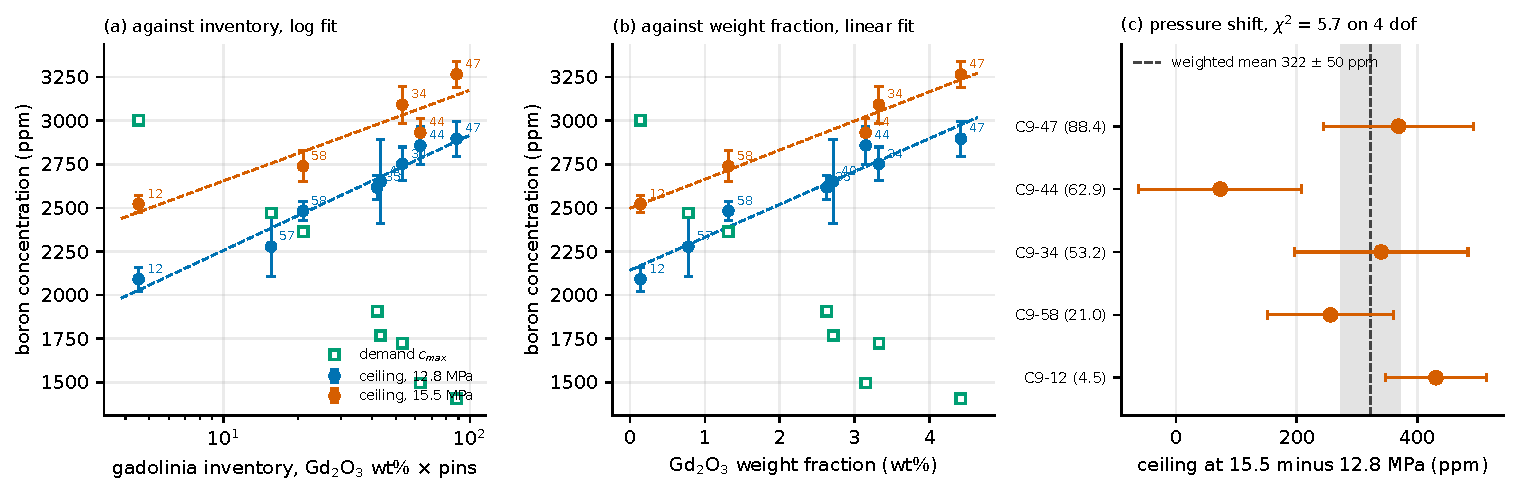
\includegraphics[width=\textwidth]{images/c9_ceiling_two_pressures}
  \caption{Boron ceiling at both pressures against the gadolinia loading.}
  \label{fig:c9-ceiling-2p}
\end{figure}

The ceiling rises with the gadolinia loading at both pressures, and two
measures of that loading were tested:

\begin{itemize}
  \item At \SI{12.8}{MPa} the Spearman coefficient is 1.000 against the
        inventory and 0.976 against the Gd$_2$O$_3$ weight fraction.

  \item At \SI{15.5}{MPa} it is 0.900 against the inventory and 1.000
        against the weight fraction.

  \item The number of gadolinia pins alone shows no correlation at
        either pressure, with coefficients of $-0.07$ and $-0.10$.
\end{itemize}

The two measures rank every lattice identically except C9-34 and C9-44.
Their ceilings differ by \SI{106(146)}{ppm} at \SI{12.8}{MPa}, in favour
of C9-44, and by \SI{161(133)}{ppm} at \SI{15.5}{MPa}, in favour of
C9-34, so this pair is not ordered by either measurement. The present
data therefore do not distinguish the inventory from the weight fraction
as the governing variable.

An unweighted logarithmic fit in the inventory gives the relation below.

\begin{equation}
  c_\mathrm{MTC}(I) = a \ln I + b
  \label{eq:mtc-ceiling-fit}
\end{equation}

\noindent where the symbols have the following meaning:

\begin{itemize}
  \item $c_\mathrm{MTC}$ is the boron concentration at which the
        moderator temperature coefficient crosses zero, in ppm.

  \item $I$ is the gadolinia inventory, the Gd$_2$O$_3$ weight fraction
        in wt\% multiplied by the number of gadolinia pins as built,
        dimensionless.

  \item $a$ is the slope, \SI{287}{ppm} at \SI{12.8}{MPa} and
        \SI{226}{ppm} at \SI{15.5}{MPa}.

  \item $b$ is the intercept, \SI{1595}{ppm} at \SI{12.8}{MPa} and
        \SI{2134}{ppm} at \SI{15.5}{MPa}.
\end{itemize}

The root mean square residual of this fit is \SI{55}{ppm} at
\SI{12.8}{MPa} and \SI{96}{ppm} at \SI{15.5}{MPa}. A straight line in
the weight fraction gives \SI{68}{ppm} and \SI{48}{ppm}. Neither form is
preferred at both pressures.

The pressure shift is consistent with a single value. Over the five
lattices measured twice its weighted mean is \SI{322(50)}{ppm}, with
$\chi^2 = 5.7$ on four degrees of freedom ($p = 0.22$), and no trend
with inventory is resolved.

The verdicts do not depend on the pressure. C9-12 fails its own ceiling
by \SI{912}{ppm} at \SI{12.8}{MPa} and by \SI{481}{ppm} at
\SI{15.5}{MPa}. C9-58 clears by \SI{120}{ppm} and \SI{376}{ppm}, so its
binding pressure is \SI{12.8}{MPa}. The three front designs measured at
both pressures clear by 1027 to \SI{1491}{ppm} at \SI{12.8}{MPa} and by
1367 to \SI{1860}{ppm} at \SI{15.5}{MPa}.

The ceiling and the demand also move in opposite directions with the
same variable. Across the eight lattices at \SI{12.8}{MPa} the ceiling
spans \SI{806}{ppm}, while the operating margin spans \SI{2403}{ppm},
from \SI{-912}{ppm} to \SI{+1491}{ppm}. The demand does most of the work
and the ceiling reinforces it, so a design is either comfortably
operable or clearly not, with little middle ground.

\paragraph{The fidelity of the two sides of the comparison.}
The ceiling is measured on the three-dimensional core model, while the demand is a
two-dimensional core quantity, so the comparison in this section mixes two
fidelities. The rodded confirmation of Section~\ref{sec:res-c9-front}
measures the size of that mismatch. At each design's own critical
concentration the unrodded factor falls from 1.0000 in two dimensions to
0.9704 on the three-dimensional core model, a reactivity difference of 3001 to
\SI{3028}{pcm} across the five front designs, which at their measured boron
worths is 445 to \SI{459}{ppm}.

The three-dimensional demand is therefore about \SI{450}{ppm} below the value
in Table~\ref{tab:c9-front}, and the two-dimensional ceiling is about
\SI{480}{ppm} below the three-dimensional one. Both errors point the same
way, so every margin quoted here is conservative by roughly \SI{900}{ppm}.
The direction of the conclusions is unaffected. The comparison is stated as
it was measured and is not corrected, because a correction would mix a
measured quantity with an inferred one, and a campaign that relied on this
comparison would have to measure both sides on the same model.

\paragraph{Verdicts.}
Of the seven candidates on either peaking front, six clear their own ceiling
and one does not:

\begin{itemize}
  \item C9-47, C9-44, C9-34, C9-40 and C9-35 clear it by 710 to
        \SI{1491}{ppm}, which is 3.7 standard deviations or more. These
        verdicts are not in question.

  \item C9-58 clears by \SI{120}{ppm}, which is 2.3 standard deviations.
        Its ceiling combines two scans, a four-point sweep from 0 to
        \SI{3000}{ppm} and a four-point sweep inside 2200 to
        \SI{2800}{ppm}, which agree with $\chi^2 = 0.86$ on one degree of
        freedom and give \SI{2483}{ppm} together. Further sampling will
        not change the verdict, because the margin itself is the result:
        this design operates at \SI{95}{\%} of what its lattice
        tolerates, against \SI{49}{\%} for C9-47. Its operability is
        therefore not established by this campaign in the sense the other
        five members are.

  \item C9-12 fails it by \SI{912}{ppm}, 13.2 standard deviations. It is the
        one design that entered the front only through the
        three-dimensional peaking of Section~\ref{sec:res-c9-peaking}, and
        it is inoperable whatever its peaking.
\end{itemize}

C9-57, the diagnostic design, fails by \SI{193}{ppm} at 1.1 standard
deviations, and the fidelity mismatch above works in its favour by about
\SI{450}{ppm}, so it would clear on a consistent three-dimensional
comparison. Its verdict is undecided on both counts and is reported as
such. It is not a front candidate and nothing in this chapter depends on
it, but it marks where the combined effect of demand and ceiling places
the boundary, at roughly \SI{1}{wt\%} of gadolinia in this design space.

C9-12 is the only verdict the mismatch cannot overturn. It fails by
\SI{912}{ppm} on the comparison as measured and by roughly \SI{460}{ppm}
once both sides are put on the three-dimensional core model, which is still more than
four standard deviations. The eight lattices also confound the inventory with the
reflector thickness, which is at its bound for seven of the eight, so the
logarithmic law should not be extrapolated outside the converged region of
this campaign.

\subsection{Status of the post-analysis}
\label{sec:res-c9-post}

The post-analysis of Campaign 9 mirrors that of Campaign 8 and is scripted
in \texttt{run\_c9\_post.sh}. The three-dimensional peaking of the front and
of the whole archive with all rods out is reported in
Section~\ref{sec:res-c9-peaking}, the rodded three-dimensional confirmation
of the front in Section~\ref{sec:res-c9-front}, and the boron ceiling of
eight candidate lattices in Section~\ref{sec:res-c9-ceiling}.

The burnup dependence of the Route B k-target leakage factor, which relates
the assembly multiplication factor to the core one and includes the axial
contribution, was measured on the five front designs with the method of
Section~\ref{sec:res-kt-burnup}. Table~\ref{tab:c9-kt-burnup} gives the
result. The two-dimensional to three-dimensional axial factor of
Section~\ref{sec:res-c9-front} is a different quantity and is measured at
beginning of life only.

\begin{table}[htbp]
  \centering
  \small
  \caption{Campaign 9 front: burnup dependence of the Route B leakage factor.}
  \label{tab:c9-kt-burnup}
  \setlength{\tabcolsep}{4.2pt}
  \begin{tabular}{cccccccc}
    \toprule
    Design & $t_\mathrm{refl}$ & $B_\mathrm{EOC}$ & $\mathrm{LF}_\mathrm{BOL}$ &
      $\mathrm{LF}_\mathrm{EOC}$ & $r_\mathrm{EOC}$ & drift &
      $\Delta\mathrm{EFPD}$ \\
    {[--]} & [cm] & [MWd/kgHM] & [--] & [--] & [pcm] & [pcm] & [d] \\
    \midrule
    C9-47 & 5.66 & 19.8 & 1.0823 & 1.0822 & $+15$ & $-17 \pm 194$ & $-2$ \\
    C9-44 & 5.66 & 18.4 & 1.0840 & 1.0830 & $+92$ & $-94 \pm 105$ & $-13$ \\
    C9-34 & 5.66 & 17.8 & 1.0843 & 1.0831 & $+98$ & $-118 \pm 105$ & $-17$ \\
    C9-40 & 5.66 & 18.3 & 1.0823 & 1.0826 & $+51$ & $+23 \pm 109$ & $-6$ \\
    C9-35 & 5.65 & 19.2 & 1.0832 & 1.0824 & $+39$ & $-70 \pm 137$ & $-4$ \\
    \bottomrule
  \end{tabular}
\end{table}

The drifts combine by inverse-variance weighting into a mean of
$-62 \pm 54$\,pcm, with $\chi^2/\nu = 0.26$ over the five designs. The mean is
consistent with zero at 1.2 standard deviations and with the $-13 \pm 30$\,pcm
of the Campaign 8 designs, Equation~\eqref{eq:kt-comp}. The leakage factor
fitted at beginning of life therefore holds to the end of cycle, which is
what justifies the depletion at assembly level.

The residuals behave differently. All five are positive, from $+15$ to
$+98$\,pcm with a mean of $+59$\,pcm, so the measured factor lies above the
tabulated target on every design. Five residuals of the same sign are a
systematic offset in the k-target table and are stated separately from the
drift. The offset is small, about one part in two thousand in the factor,
and it shortens the reported cycle by 2 to 17 days, below one per cent.

C9-34 is the design for which the correction is largest relative to its
margin. Its cycle length of \SI{1841}{d} becomes \SI{1824}{d} once the
end-of-cycle leakage factor is applied, that is \SI{2}{d} below the mission
floor. The correction itself carries an uncertainty of about \SI{15}{d},
propagated from the \SI{105}{pcm} uncertainty of its drift, so the shortfall
is \SI{2+-15}{d} and is not resolved. It is also an order of magnitude
smaller than the \SI{37}{d} uncertainty of the cycle-length proxy at this
mission. The design is therefore retained on the front, with the same caveat
that applies to C9-44, that its compliance with the mission is not
established by this campaign.

Corrections are not applied retroactively to individual designs, because
the front is the set the constraint evaluation produced. A correction
applied to one design and not to the other fifty-nine would not correspond
to any consistent procedure.

The following stages were not complete when this chapter was written:

\begin{enumerate}
  \item The boron ceiling at \SI{15.5}{MPa} on C9-34 and C9-44.

  \item An independent measurement of the boron worth.
\end{enumerate}

\subsection{Limitations}
\label{sec:res-c9-limits}

Six limitations qualify the result of this campaign.

\begin{enumerate}
  \item The reflector is active at its bound. Every front member carries
        the largest reflector the vessel admits, and
        Figure~\ref{fig:c9-design-space} shows that the optimiser reached
        the bound in the first infill iteration and did not test a design
        away from it afterwards. The front is a boundary optimum,
        conditional on the vessel envelope and the clearance of
        Section~\ref{sec:meth-c8-space}.

  \item The cycle-length margin lies inside the proxy uncertainty. The
        front members deliver 1841 to \SI{1947}{d} against a floor of
        \SI{1826}{d}, margins of 15 to 121 days. The core-level validation
        of Section~\ref{sec:res-corevalidation} places the cycle-length
        proxy at about the \SI{2}{\%} level, \SI{37}{d} at this floor, so
        C9-34 and C9-44, at 15 and 32 days, cannot be asserted to meet it.

  \item The boron ceiling is measured at one pressure.
        Section~\ref{sec:res-c9-ceiling} scans eight lattices at
        \SI{12.8}{MPa}, and every candidate on either peaking front except
        C9-12 clears its own ceiling. Only C9-47 is scanned at
        \SI{15.5}{MPa}, and that scan has three points instead of four, so
        it carries no refit uncertainty. The ceiling at the higher pressure
        is therefore known for one design and assumed for the others, and C9-58 clears its own ceiling by only \SI{120}{ppm}, so its
        operability is not established.

  \item Three of the five front members lie inside the noise. Only C9-47
        and C9-34 survive every resample of Table~\ref{tab:c9-stability},
        and the apparent quality of the front is optimistic by \SI{2.8}{\%}
        in hypervolume through selection alone.

  \item The peaking objective is evaluated in two dimensions and at campaign
        fidelity, and a front this narrow is sensitive to both. Raising the
        statistics lowers the hot channel factor by $0.013 \pm 0.004$ on
        the front designs, the three-dimensional model shifts it further by
        an amount that depends on the design, and substituting the
        three-dimensional value changes the non-dominated set in two
        measured ways (Section~\ref{sec:res-c9-peaking}). The front of
        Table~\ref{tab:c9-front} is therefore a set of comparable designs
        and not an ordered ranking.

  \item The depletion runs at a constant \SI{1000}{ppm}, as in every
        campaign, so every cycle length remains a lower bound for a core
        operated with boron letdown, and the critical concentration is
        measured at two states of the cycle only.
\end{enumerate}

Limitations 3 and 5 were the two that could change a conclusion, and both
are now measured. Section~\ref{sec:res-c9-ceiling} gives the ceiling of eight
lattices at \SI{12.8}{MPa} and of C9-47 at both pressures, and
Section~\ref{sec:res-c9-peaking} compares the two- and three-dimensional
peaking over all sixty designs. Neither displaces the selected design, and
the checks that remain are listed in Section~\ref{sec:res-c9-post}.


% =====================================================================
%  conclusions.tex
%  Revised 13 September 2026 for the inclusion of Campaign 9.
%  Labels defined: ch:conclusions, sec:concl-answer, sec:concl-reform,
%  sec:concl-candidates, sec:concl-limits, sec:concl-future,
%  eq:concl-reform, tab:concl-future.
%  Style: short paragraphs, no semicolons, no em dashes, formulas alone
%  with term lists, enumerations as lists.
% =====================================================================

\chapter{Conclusions}
\label{ch:conclusions}

\section{Summary of the study and its findings}
\label{sec:concl-answer}

The study asked which core designs a LABGENE-class pressurised water
reactor of \SI{48}{MW} thermal could adopt when the only information
available is the open record. It answered by building a
surrogate-assisted multi-objective optimisation around a Monte Carlo
model of the core and running it through nine campaigns, 636
evaluations in all. Each campaign changed one element of the method and
measured its effect. Campaigns 1 to 8 maximised the cycle length and
minimised the radial peaking factor. The eighth produced a front of
eight designs and a second set of four designs controllable with two
regulating banks, and the difference between the two sets led to the
reformulated problem of Campaign 9.

Four findings carry the weight.

\begin{enumerate}
  \item A derived bound is never a substitute for a measured
        constraint. The reactivity ceiling of Campaigns 1 to 6 was
        replaced in Campaign 7 by a directly measured controllability
        screen, and the comparison showed the derived ceiling
        rejecting fourteen designs whose own measured bank worth made
        them controllable (Section~\ref{sec:res-c7-screens}). Campaign
        8 reversed the nesting so that the measurement does the work
        and the bound is inert. The retrospective derivation also gave
        the historic ceiling of 1.35 its provenance, as the all-bank
        controllability bound of this core to within two per cent.

  \item The finite-height correction is a constant of the geometry.
        The axial leakage factor varies by \SI{160}{pcm} over a factor
        of two in excess reactivity, so a single value corrects the
        whole design space and every cycle length of Campaigns 8 and 9
        refers to a finite-height core (Section~\ref{sec:meth-lax}).

  \item The cycle length of this core is a requirement to be met. Every
        Campaign 8 design exceeded the reported refuelling interval,
        and the excess reactivity spent on the longer cycle had to be
        held by the control rods (Section~\ref{sec:concl-reform}).

  \item At the required cycle length, the boron the core needs falls
        with its gadolinia loading. Among the feasible Campaign 9
        designs between 4.15 and \SI{4.55}{wt\%}, the critical
        concentration at the most reactive state falls from 3003 to
        \SI{1406}{ppm} as the gadolinia rises from 0.14 to
        \SI{4.42}{wt\%} (Section~\ref{sec:res-c9-gd}), a trade that the
        objectives of the first eight campaigns could not reward.
\end{enumerate}

\section{Reformulation of the cycle length as a constraint}
\label{sec:concl-reform}

The optimisation was posed, from the first campaign, as the
maximisation of cycle length against the minimisation of the radial
peaking factor. That is the natural formulation for a naval core,
whose defining advantage is time between refuellings, and it was kept
through eight campaigns so that the campaigns remain comparable.
Campaign 8 showed that it is the wrong formulation for the final design
choice, for a reason that only became visible once controllability was
measured rather than assumed.

The open record gives the prototype a refuelling interval of five
years~\cite{dinizcosta_2017}. Through Equation~\eqref{eq:mission-efpd} that interval
corresponds to 913 to 1461 effective full power days for capacity
factors between 0.5 and 0.8, and no open source states the capacity
factor. Every design on the Campaign 8 front exceeds the upper end of
that range, the shortest by a third and the longest by a factor of
four (Section~\ref{sec:res-c8-mission}). The objective kept pushing
cycle length long after the requirement was met, and it could only do
so by raising the beginning-of-life excess reactivity, because a
longer cycle is bought with reactivity to be burned later.

That excess has to be held by something at the start of life. In this
model the soluble boron and the gadolinia are already present in every
eigenvalue, so what remains is held by the control rods. Every design
on the front needs the four regulating banks to hold between
\num{8930} and \SI{13627}{pcm} at power, which means banks inserted
deep into the core throughout early life. A pressurised water reactor
does not operate that way. Its regulating banks sit near the withdrawn
position at power and carry only the power defect and the manoeuvring
band, while the excess is held by boron adjustment and by burnable
absorber whose burnout tracks the fuel. The four Campaign 8 designs
that behave that way, controllable by two banks and holding \num{2564}
to \SI{4068}{pcm}, still deliver 1142 to 3381 effective full power
days (Section~\ref{sec:res-c8-split}).

The requirement on cycle length is a floor. A cycle beyond it gives the
mission nothing and costs excess reactivity that the control system
must absorb. The peaking factor and the reactivity to be held at
start-up have no such floor, and both improve in the direction of the
design goal for as long as the search can move them. Those are the
objectives, and the cycle length belongs among the constraints, at the
value the mission requires. Campaign 9 was posed that way.

\begin{equation}
\begin{aligned}
\min_{\mathbf{x}}\ &\big(F_{\Delta H}(\mathbf{x}),\ c_\mathrm{max}(\mathbf{x})\big) \\
\text{subject to}\ &\mathrm{EFPD}(\mathbf{x}) \ge \mathrm{EFPD}_\mathrm{req},\quad
g_j(\mathbf{x}) \le 0
\end{aligned}
\label{eq:concl-reform}
\end{equation}

\noindent where the symbols have the following meaning.

\begin{itemize}
  \item $F_{\Delta H}$ is the radial enthalpy-rise hot channel factor
        with all rods out, dimensionless, the first objective.

  \item $c_\mathrm{max}$ is the soluble boron concentration at which
        the core is critical at the most reactive state of its cycle,
        in ppm, the second objective, defined in
        Equation~\eqref{eq:c9-cmax}.

  \item $\mathrm{EFPD}_\mathrm{req}$ is the required cycle length,
        1826 effective full power days, five years at a capacity factor
        of one, the conservative choice of Section~\ref{sec:meth-c9}.

  \item $g_j$ are the remaining constraints of
        Section~\ref{sec:meth-c9}: the reactivity window, the
        enrichment cap, the vessel fit, the peaking screen at 1.65, and
        the control screen at beginning of life and at the operating
        maximum.
\end{itemize}

The second objective carries the reactivity that the Campaign 8 front
could not hold. The critical concentration at the operating maximum
expresses the beginning-of-life excess and the gadolinium hump in one
quantity, and it does so in the unit in which the moderator
temperature coefficient bounds it: a design whose critical
concentration exceeds the boron ceiling of
Section~\ref{sec:res-c8-mtc} cannot be held at power by boron with a
non-positive coefficient.

Scored on the Campaign 8 archive without transport, the reformulated
problem at the five-year floor selects designs 47 and 13
(Section~\ref{sec:res-c8-retro}). Campaign 9 then searched the same
design space with the boron measured on every design. Its front holds
five designs at peaking factors of 1.490 to 1.545 and boron demands of
1406 to \SI{1908}{ppm}, every one within 121 days of the floor, so the
constraint binds (Section~\ref{sec:res-c9-front}). At that floor the
enrichment of the front is 4.2 to \SI{4.5}{wt\%}, below the 6 to
\SI{8}{wt\%} stated for the prototype in 2014 and far below the
\SI{19}{wt\%} reported in 2025.

\section{Candidate designs}
\label{sec:concl-candidates}

The two formulations give two stages of candidate.

Under the formulation of Campaigns 1 to 8, the candidate is design 47
of Table~\ref{tab:c8-front}, the low-peaking floor of the front
(Section~\ref{sec:res-c8-decision}). Its cycle length is 1941\,EFPD,
reproduced within 1.5 per cent by a replicate depletion, and its
radial peaking factor is 1.510, with a seed-to-seed standard deviation
of about 0.014 at the archive fidelity that does not separate it from
its three nearest neighbours on that axis. On the three-dimensional
core model with structural components at 1000\,ppm it holds a two-bank margin of
1330\,pcm, which the gadolinium hump leaves intact because beginning of
life is its most reactive state. Its differential boron worth is
6.98\,pcm per ppm, its rods-only margin under the four regulating
banks with no boron is 3069\,pcm, and its critical concentration of
\SI{2327}{ppm} lies below the boron ceiling at both primary conditions
(Sections~\ref{sec:res-c8-boron}, \ref{sec:res-c8-zeroboron}
and~\ref{sec:res-c8-mtc}). Design 53 holds more margin and needs less
boron but meets five years only at a capacity factor of 0.8, and design
31 loses its two-bank margin at the maximum of its hump.

On the objectives of Campaign 9, both Campaign 8 designs selected by
the retrospective are dominated by members of the Campaign 9 front.
Design 47 of Campaign 8 needs 419 to \SI{602}{ppm} more boron than
designs 35, 40 and 34 of Campaign 9, at a peaking factor that differs
by less than one and a half seed standard deviations, and design 13 is
dominated by designs 47 and 44 of Campaign 9 on both objectives
(Section~\ref{sec:res-c9-compare}). The comparison uses critical
concentrations obtained by different routes and is indicative until the
two archives are scored on the same footing.

Within Campaign 9 the champion is C9-47, the lowest boron demand of the
front, and C9-47 and C9-34 are the only members that stay on the front
in every resample of the measurement noise
(Section~\ref{sec:res-c9-convergence}). Two further designs, C9-29 and
C9-30, are excluded from the nominal front by less than the noise, so the
candidate set of the campaign holds seven designs. Four of the five front
members, C9-47 among them, would have been buried two to four fronts deep
under the cycle-length objectives (Section~\ref{sec:res-c9-discarded}).

Re-solved with all rods out on the three-dimensional model, C9-47 and
C9-34 stay on the front. C9-40 enters it, because its peaking factor
falls by 0.040, and C9-44 leaves it, because C9-47 then has both the lower
peaking and the lower boron demand. Both changes exceed four standard
deviations of the seed noise, but the one that brings C9-40 in rests on
the design with the largest seed spread of the five
(Section~\ref{sec:res-c9-peaking}). Neither C9-47 nor C9-34 is yet a final
candidate. Three of the checks that the Campaign 8 designs passed are now passed by
the Campaign 9 front. On the three-dimensional model with structural
components, at each design's own critical
concentration, the first two regulating banks hold every front member
subcritical with 9228 to \SI{9545}{pcm} of margin
(Section~\ref{sec:res-c9-front}), and the boron ceiling measured on the
lattice of each candidate is cleared, by \SI{1491}{ppm} for C9-47 and
\SI{1027}{ppm} for C9-34 (Section~\ref{sec:res-c9-ceiling}). The k-target
leakage factor of every front design is constant over the cycle within its
uncertainty (Section~\ref{sec:res-c9-post}). Until the remaining checks of
that section are closed, design 47 of Campaign 8 is the most completely confirmed
design of the study, and the Campaign 9 front is the set from which the
final choice will be made.

\section{Limitations}
\label{sec:concl-limits}

\begin{enumerate}
  \item The model is a two-dimensional beginning-of-life core in the
        optimisation loop, corrected for axial leakage by a measured
        constant. On the eleven Campaign 8 designs the
        three-dimensional core model gives the peaking, the rod worth
        and the axial leakage with rods withdrawn and inserted, and
        shows that the leakage correction of the unrodded core does not
        hold for the rodded core. On the five Campaign 9 front designs
        it gives the peaking, the axial power shape, the bank worth and
        the axial rod worth curves. No depletion was run in three
        dimensions in any campaign.

  \item The control screen tests hold-down at power with the operating
        boron present and no xenon. It is not a shutdown-margin
        demonstration, which needs the cold state, all assemblies
        minus the highest-worth one, and a stated margin.

  \item Up to Campaign 8 the reactivity swing over the cycle was not
        penalised. The optimiser removed burnable absorber wherever it
        could, and humps of several thousand pcm appear in the depletion
        histories. Campaign 9 scores the boron demand at the operating
        maximum and applies the control screen there, which closes this
        limitation for the last campaign only.

  \item Every cycle length comes from a depletion at a constant
        \SI{1000}{ppm} and is a lower bound for a core operated with
        boron letdown.

  \item The statistical error on the peaking objective was not
        measured during the campaigns, only bounded. Measured afterwards
        at the confirmation statistics, it is 0.011 on the Campaign 8
        designs and 0.0061 on the Campaign 9 front, and the ordering of
        neighbouring front designs on that axis is not resolved in
        either campaign. The peaking objective is also two-dimensional,
        and on the Campaign 9 front the three-dimensional value changes
        which designs are non-dominated.

  \item Every design below a pitch of \SI{1.2242}{cm} in Campaigns 1
        to 7 carried clipped guide tubes. Campaigns 8 and 9 are free of
        the defect and the earlier results are caveated.

  \item Thermal-hydraulic feedback is absent. Temperatures are fixed at
        representative hot full power values, so no departure from
        nucleate boiling ratio and no fuel temperature limit is
        evaluated. The moderator temperature coefficient was evaluated
        outside the loop, on one Campaign 8 design and on eight
        Campaign 9 lattices, and enters only through the boron ceiling.

  \item The boron ceiling was measured on the lattice of Campaign 8
        design 47, with \SI{2.88}{wt\%} gadolinia on twelve rods. The
        Campaign 9 front carries 2.6 to \SI{4.4}{wt\%} on 16 or 20
        rods, so the ceiling is a reference for that front until it is
        measured on its own lattice.
\end{enumerate}

\section{Continuation of this work}
\label{sec:concl-future}

The work stops where the deadline put it, with the post-analysis of
Campaign 9 in progress. Table~\ref{tab:concl-future} lists the
continuations in the order they would be taken up, each with what it
needs and what it would settle.

\begin{table}[htbp]
  \centering
  \footnotesize
  \caption{Continuations of the study, in order of priority.}
  \label{tab:concl-future}
  \begin{tabularx}{\textwidth}{@{}>{\raggedright\arraybackslash}p{3.6cm}>{\raggedright\arraybackslash}X>{\raggedright\arraybackslash}p{4.0cm}@{}}
    \toprule
    Continuation & What it involves & What it settles \\
    \midrule
    Campaign 9 post-analysis
      & Boron ceiling at 15.5\,MPa on C9-34 and C9-44, independent boron worth
      & The final candidate \\
    \addlinespace
    Shutdown margin
      & Cold zero-power state, all 32 assemblies minus the highest-worth one, operating boron, margin of at least about \SI{1600}{pcm}
      & Whether the candidates meet a licensing-style shutdown criterion rather than an operating one \\
    \addlinespace
    Boron letdown in the depletion
      & A critical boron search at each burnup step in place of the constant \SI{1000}{ppm}
      & Cycle lengths of an operated core in place of lower bounds \\
    \addlinespace
    Core-level depletion
      & Depletion of the core in place of the reflected assembly, at the cost estimated in Section~\ref{sec:meth-dep-level}
      & The radial burnup distribution, and the removal of the leakage-corrected target approximation \\
    \addlinespace
    Burnable absorber design
      & Mixed gadolinia concentrations per assembly, enriched gadolinium, or erbia, following the soluble-boron-free literature cited in the review
      & A flatter swing at the same cycle length, and the path to a boron-free variant \\
    \addlinespace
    Peaking uncertainty in the loop
      & Read the core tally errors on every evaluation and carry them into the surrogate as noise
      & Statistically resolved ordering of the front on the peaking axis \\
    \addlinespace
    Acquisition robustness
      & A per-variable minimum spread in the batch selection, so that a batch cannot satisfy the separation rule by moving two variables
      & Ends the collapse mode seen in Campaigns 6 and 7 \\
    \addlinespace
    Thermal-hydraulic coupling
      & OpenMC coupled to a subchannel or porous-medium solver, in the frameworks surveyed in the review
      & Coupled temperature feedback, departure from nucleate boiling, and fuel temperature margins on the candidates \\
    \addlinespace
    Multi-batch loading
      & Reload strategy and loading-pattern optimisation for a core that refuels rather than replaces
      & The peaking gap between a single-batch uniform core and licensed practice \\
    \bottomrule
  \end{tabularx}
\end{table}

The first continuation is scripted and was running when this chapter
was written. Its last stage is the gate for any further campaign. If
the ratio of three- to two-dimensional peaking is constant across the
Campaign 9 archive, the three-dimensional objective is a monotone
transform of the two-dimensional one, the front does not move and no
further campaign is needed. On the eleven Campaign 8 designs the ratio
was not constant, with a Spearman coefficient of 0.909 and a largest
swap of three positions. On the five Campaign 9 front designs the ratio
is 0.992 with a standard deviation of 0.014, and substituting it already
changes the non-dominated set of those five, so the measurement on all
60 designs is what decides whether a three-dimensional campaign is
needed.

The study set out to show that a core can be designed from four open
facts and a declared design space, and that a surrogate-assisted loop
can carry the search at a cost a workstation affords. Both were shown
within the limits stated above: a two-dimensional beginning-of-life
model in the loop, a fresh single-batch core, fixed temperatures and a
constant boron concentration in the depletion. Within those limits the
framework produced a front of buildable, controllable designs, the
finding that the cycle length of this core is a requirement to be met,
and a reformulated campaign whose front meets that requirement with
less boron than the two Campaign 8 designs selected by the same
formulation. What lies beyond the limits, the three-dimensional power
shape of the new front, the shutdown margin, the thermal-hydraulic
feedback and the reload strategy, is the work of
Table~\ref{tab:concl-future}, and the archive, the checkpoints and the
scripts that would carry it out are in place.


\begin{appendices}

% =====================================================================
%  appendix_model_inputs.tex
%  Appendix A: record of every input value of the reactor model.
%  Values read from the simulation repository, branch main, commit
%  e4a3582 (8 September 2026). Formulas are given in the main text.
% =====================================================================

\chapter{Record of the model input data}
\label{app:model-inputs}
\label{app:labgene-data}

\section{Reading key}
\label{app:inputs-purpose}

This appendix records the value of every input of the reactor model,
its origin, and whether it was validated in this thesis. The formulas
that use these values are given in the main text. All values were read
from the simulation repository, branch \texttt{main}, commit
\texttt{e4a3582}, the state described in
Appendix~\ref{app:code-architecture}. The codes of the tables are given
in Table~\ref{tab:in-key}.

\begin{table}[htbp]
  \centering
  \small
  \caption{Codes of the input tables.}
  \label{tab:in-key}
  \begin{tabularx}{\textwidth}{@{}l>{\raggedright\arraybackslash}X@{}}
    \toprule
    Code & Meaning \\
    \midrule
    BRZ & Stated by the Brazilian Navy or the Brazilian government \\
    LIT & Stated in a peer-reviewed article, a laboratory report or a code manual \\
    REF & Taken from the NuScale-class reference benchmark adopted as design analog \\
    INF & Inferred from open information that does not state the value directly \\
    EST & Engineering estimate of this work \\
    NUM & Numerical setting with no physical counterpart \\
    DER & Derived from other entries \\
    \midrule
    V = Y & Confirmed by a verification calculation of this thesis \\
    V = P & Bounded by a sensitivity calculation of this thesis, not confirmed \\
    V = N & Adopted as given, not verified in this thesis \\
    \bottomrule
  \end{tabularx}
\end{table}

% =====================================================================
\section{Open data on the LABGENE prototype}
\label{app:inputs-labgene}

Table~\ref{tab:labgene-data} records the open information on the
LABGENE prototype used in this thesis. Four model inputs are anchored
to it: the reactor type, the thermal power, the enrichment class and the
vessel inner radius. Every other input is taken from the NuScale-class
reference benchmark (REF) or estimated in this work (EST).

\begin{table}[htbp]
  \centering
  \footnotesize
  \caption{Open-source data on the LABGENE prototype.}
  \label{tab:labgene-data}
  \begin{tabularx}{\textwidth}{@{}>{\raggedright\arraybackslash}p{3.2cm} >{\raggedright\arraybackslash}p{3.8cm} >{\raggedright\arraybackslash}X@{}}
    \toprule
    \textbf{Item} & \textbf{Value adopted} & \textbf{Source} \\
    \midrule
    Reactor type & PWR & \cite{ctmsp_labgene_2015,vasconcelos_fapesp_2025} \\
    Rated power & 48\,MW thermal & \cite{demartini_nuclep_2022}, 48\,MWth or 11\,MWe in \cite{galante_podernaval_2020}, 48 to 50\,MWth in \cite{dinizcosta_2017} \\
    Fuel & UO$_2$ pellets in rods grouped into fuel elements & \cite{marinha_inb_labgene_2022,pereira_rmb_2023} \\
    Enrichment class & LEU, below 20\,wt\% & \cite{brazil_npt_wp71_2022,brazil_npt_wp13_2026}, definition \cite{nrc_10cfr110_2} \\
    Enrichment value & Searched, up to 13.913\,wt\% in Campaigns 8 and 9 & 6 to 8\,wt\% \cite{dinizcosta_2017}, 18 to 19\,wt\% \cite{kassenova_2014}, up to 19\,wt\% \cite{vasconcelos_fapesp_2025} \\
    Refuelling interval & Objective in Campaigns 1 to 8, 1826\,EFPD constraint in Campaign 9 & Five years \cite{dinizcosta_2017} \\
    Vessel inner radius & 90\,cm & \cite[Fig.~13]{maruyama_2013} \\
    Vessel wall and height & 10\,cm and 470\,cm, not in the two-dimensional model & \cite[Fig.~13]{maruyama_2013} \\
    Active fuel height & 120\,cm, estimate & Proportions of \cite[Fig.~13]{maruyama_2013} \\
    Lattice, pitch, assembly count, absorbers, boron, reflector & Estimates of this thesis & No open source \\
    Plant status & Not critical as of May 2025, installations 66.8\,\% complete at the end of 2025 & \cite{vasconcelos_fapesp_2025,marinha_relatorio_gestao_2025} \\
    Safeguards status & Special procedures under Article~13 of the Quadripartite Agreement in negotiation & \cite{iaea_dg_statement_2022,eu_statement_bog_2025,brazil_npt_wp13_2026} \\
    \bottomrule
  \end{tabularx}
\end{table}

% =====================================================================

\section{Vessel, core envelope and reflector}
\label{app:inputs-vessel}

\small
\setlength{\tabcolsep}{3pt}
\begin{longtable}{@{}>{\raggedright\arraybackslash}p{3.25cm} >{\raggedright\arraybackslash}p{2.65cm} >{\raggedright\arraybackslash}p{1.15cm} >{\raggedright\arraybackslash}p{1.1cm} >{\raggedright\arraybackslash}p{3.85cm} >{\raggedright\arraybackslash}p{0.4cm} >{\raggedright\arraybackslash}p{0.95cm}@{}}
\caption{Vessel, core envelope and reflector.}
\label{tab:in-vessel} \\
\toprule
\textbf{Parameter} & \textbf{Value} & \textbf{Unit} & \textbf{Code} &
\textbf{Source} & \textbf{V} & \textbf{Note} \\
\midrule
\endfirsthead
\toprule
\textbf{Parameter} & \textbf{Value} & \textbf{Unit} & \textbf{Code} &
\textbf{Source} & \textbf{V} & \textbf{Note} \\
\midrule
\endhead
\bottomrule
\endlastfoot
Vessel inner radius & 90.0 & cm & INF & \cite[Fig.~13, p.~50]{maruyama_2013} & N & (a) \\
Vessel wall thickness & 10.0 & cm & INF & \cite[Fig.~13]{maruyama_2013} & N & (b) \\
Vessel height & 470 & cm & INF & \cite[Fig.~13]{maruyama_2013} & N & (b) \\
Core barrel thickness & 5.08 & cm & REF & \cite{fridman_nuscale_benchmark_2023} & P & \\
Downcomer allowance & 2.0 & cm & EST & This work & P & (c) \\
Reserved radial clearance & 7.08 & cm & DER & Barrel plus downcomer & Y & \\
Lattice-corner pad & 0.02 & cm & NUM & This work & Y & (d) \\
Core map & 32 assemblies, $6\times6$ minus corners & -- & INF & This work & P & (e) \\
Fuel envelope radius at 1.26\,cm & 77.231 & cm & DER & Equation~\eqref{eq:renv} & Y & \\
Largest reflector thickness at 1.26\,cm & 5.669 & cm & DER & Equation~\eqref{eq:ggeom} & Y & \\
Active fuel height & 120.0 & cm & INF & Proportions of \cite[Fig.~13]{maruyama_2013} & P & (f) \\
Radial reflector material & Homogenised SS304 and borated water & -- & EST & This work & P & \\
Reflector steel volume fraction & 0.90 & -- & EST & This work, 0.956 in \cite{ez_aldeen_2025} & P & (g) \\
\end{longtable}
\setlength{\tabcolsep}{6pt}
\normalsize

\noindent \textbf{Notes.}
\begin{enumerate}[label=(\alph*), nosep]
  \item Simplified structural drawing prepared for CTMSP, the only open geometric source on the prototype.
  \item Not in the two-dimensional model. Modelled only in the three-dimensional confirmation.
  \item Sensitivity to 3.7\,cm computed on the candidates only.
  \item Prevents an OpenMC surface from passing through a lattice corner. Defined once, in \texttt{core\_geometry.py}.
  \item Set by the heavy-metal mass consistent with the active height and the vessel.
  \item Enters the two-dimensional model only through the heavy-metal mass and the specific power.
  \item More moderating than the benchmark. Varied as an option in the three-dimensional confirmation.
\end{enumerate}

% =====================================================================
\section{Fuel assembly, fuel rod and guide tube}
\label{app:inputs-assembly}

\small
\setlength{\tabcolsep}{3pt}
\begin{longtable}{@{}>{\raggedright\arraybackslash}p{3.25cm} >{\raggedright\arraybackslash}p{2.65cm} >{\raggedright\arraybackslash}p{1.15cm} >{\raggedright\arraybackslash}p{1.1cm} >{\raggedright\arraybackslash}p{3.85cm} >{\raggedright\arraybackslash}p{0.4cm} >{\raggedright\arraybackslash}p{0.95cm}@{}}
\caption{Fuel assembly, fuel rod and guide tube.}
\label{tab:in-assembly} \\
\toprule
\textbf{Parameter} & \textbf{Value} & \textbf{Unit} & \textbf{Code} &
\textbf{Source} & \textbf{V} & \textbf{Note} \\
\midrule
\endfirsthead
\toprule
\textbf{Parameter} & \textbf{Value} & \textbf{Unit} & \textbf{Code} &
\textbf{Source} & \textbf{V} & \textbf{Note} \\
\midrule
\endhead
\bottomrule
\endlastfoot
Lattice & $17\times17$ & -- & REF & \cite{nuscale_htp2_2017,ez_aldeen_2025} & Y & \\
Fuel rods per assembly & 264 & -- & DER & $17^2$ minus 25 non-fuel positions & Y & \\
Guide tubes per assembly & 24 & -- & REF & Westinghouse $17\times17$ map & Y & \\
Instrumentation tubes per assembly & 1 & -- & REF & Westinghouse $17\times17$ map & Y & (a) \\
Fuel pellet outer radius & 0.406 & cm & REF & \cite{nuscale_htp2_2017,fridman_nuscale_benchmark_2023} & N & \\
Cladding inner radius & 0.414 & cm & REF & \cite{nuscale_htp2_2017,fridman_nuscale_benchmark_2023} & N & \\
Cladding outer radius & 0.475 & cm & REF & \cite{nuscale_htp2_2017,fridman_nuscale_benchmark_2023} & N & \\
Guide tube inner radius & 0.572 & cm & REF & \cite{nuscale_htp2_2017,fridman_nuscale_benchmark_2023} & N & \\
Guide tube outer radius & 0.612 & cm & REF & \cite{nuscale_htp2_2017,fridman_nuscale_benchmark_2023} & Y & (b) \\
Fuel rod pitch & 1.26 & cm & EST & Fixed from Campaign~8 & Y & (b) \\
Assembly pitch & 21.42 & cm & DER & $17\times$ rod pitch & Y & \\
Intra-assembly enrichment zones & Central $9\times9$ inner, remainder outer & -- & EST & This work & P & (c) \\
Gadolinia rod ladder & 12, 16, 20, 24, 32, 40 & rods & EST & After \cite{bae_gd_2023,epr_fsar_ch4,nuscale_htp2_2017} & P & \\
Spacer grid band height & 4.445 & cm & REF & \cite{fridman_nuscale_benchmark_2023} & P & (d) \\
Number of spacer grids & 4 & -- & EST & This work, 5 on 200\,cm in the benchmark & P & (d) \\
Spacer grid span & 41.4 & cm & EST & This work & P & (d) \\
First grid offset above fuel bottom & 3.555 & cm & REF & \cite{fridman_nuscale_benchmark_2023} & P & (d) \\
Grid strap inner box & 1.224 & cm & REF & \cite{fridman_nuscale_benchmark_2023} & Y & (b) \\
\end{longtable}
\setlength{\tabcolsep}{6pt}
\normalsize

\noindent \textbf{Notes.}
\begin{enumerate}[label=(\alph*), nosep]
  \item Modelled with the guide tube dimensions and material.
  \item Below a pitch of 1.224\,cm the lattice clips the guide-tube wall, up to 28\,\% at 1.150\,cm (Figure~\ref{fig:gt-clip}).
  \item Equal inner and outer enrichments from Campaign~8.
  \item Used only in the three-dimensional confirmation.
\end{enumerate}

% =====================================================================
\section{Material compositions and densities}
\label{app:inputs-materials}

\small
\setlength{\tabcolsep}{3pt}
\begin{longtable}{@{}>{\raggedright\arraybackslash}p{3.25cm} >{\raggedright\arraybackslash}p{2.65cm} >{\raggedright\arraybackslash}p{1.15cm} >{\raggedright\arraybackslash}p{1.1cm} >{\raggedright\arraybackslash}p{3.85cm} >{\raggedright\arraybackslash}p{0.4cm} >{\raggedright\arraybackslash}p{0.95cm}@{}}
\caption{Material compositions and densities.}
\label{tab:in-materials} \\
\toprule
\textbf{Parameter} & \textbf{Value} & \textbf{Unit} & \textbf{Code} &
\textbf{Source} & \textbf{V} & \textbf{Note} \\
\midrule
\endfirsthead
\toprule
\textbf{Parameter} & \textbf{Value} & \textbf{Unit} & \textbf{Code} &
\textbf{Source} & \textbf{V} & \textbf{Note} \\
\midrule
\endhead
\bottomrule
\endlastfoot
UO$_2$ density & 10.4 & g/cm$^3$ & REF & \cite{ezaldeen_zenodo_2025} & N & \\
(U,Gd)O$_2$ density & 10.2 & g/cm$^3$ & EST & This work & N & \\
$^{234}$U content & $0.007731\,w_{235}^{1.0837}$ & wt\% & LIT & \cite{bowman_suto_1996,scale_polaris_manual} & N & (a) \\
$^{236}$U content & 0 & wt\% & EST & Fresh uranium & N & \\
Gd$_2$O$_3$ density & 7.41 & g/cm$^3$ & LIT & Handbook value & N & \\
Gadolinium isotopic composition & Natural & -- & EST & This work & N & \\
Enrichment reduction of a gadolinia rod & 5\,\% relative per wt\% Gd$_2$O$_3$, minimum 0.2\,wt\% & -- & LIT & \cite{mildrum_segovia_2001}, minimum: this work & N & \\
Zircaloy-4 composition & Zr 98.2, Sn 1.45, Fe 0.20, Cr 0.10, O 0.05 & wt\% & REF & \cite{ezaldeen_zenodo_2025} & N & (b) \\
Zircaloy-4 density & 6.55 & g/cm$^3$ & REF & \cite{ezaldeen_zenodo_2025} & N & (b) \\
Helium gap density & 0.0015 & g/cm$^3$ & REF & \cite{ezaldeen_zenodo_2025} & N & \\
Coolant density & 0.72 & g/cm$^3$ & EST & This work & N & (c) \\
Coolant thermal scattering & \texttt{c\_H\_in\_H2O} & -- & LIT & ENDF/B-VII.1 & N & \\
Soluble boron & Natural boron, mass fraction of the water & -- & EST & This work & Y & \\
SS304 composition & Fe 69.5, Cr 19.0, Ni 9.5, Mn 2.0 & wt\% & REF & \cite{ezaldeen_zenodo_2025} & N & (b) \\
SS304 density & 7.90 & g/cm$^3$ & REF & \cite{ezaldeen_zenodo_2025} & N & (b) \\
Control rod number densities, at/(b$\cdot$cm) & From the benchmark scripts & -- & REF & \cite{ezaldeen_zenodo_2025} & N & \\
Cross-section library & ENDF/B-VII.1 & -- & LIT & \cite{chadwick_endf71_2011} & N & \\
Depletion chain & PWR chain for ENDF/B-VII.1 & -- & LIT & OpenMC, \nolinkurl{chain_endfb71_pwr.xml} & N & \\
\end{longtable}
\setlength{\tabcolsep}{6pt}
\normalsize

\noindent \textbf{Notes.}
\begin{enumerate}[label=(\alph*), nosep]
  \item Documented below 10\,wt\%. Applied up to the 16\,wt\% peripheral cap. An overestimate of $^{234}$U lowers $k$, the conservative direction.
  \item Not checked against a compendium of material compositions.
  \item IAPWS-IF97 gives 0.712\,g/cm$^3$ at 15.5\,MPa and 580\,K~\cite{wagner_iapws_if97_2000}, 1.1\,\% below the value used, a bias common to every design.
\end{enumerate}

% =====================================================================
\section{Operating conditions and power normalisation}
\label{app:inputs-operating}

\small
\setlength{\tabcolsep}{3pt}
\begin{longtable}{@{}>{\raggedright\arraybackslash}p{3.25cm} >{\raggedright\arraybackslash}p{2.65cm} >{\raggedright\arraybackslash}p{1.15cm} >{\raggedright\arraybackslash}p{1.1cm} >{\raggedright\arraybackslash}p{3.85cm} >{\raggedright\arraybackslash}p{0.4cm} >{\raggedright\arraybackslash}p{0.95cm}@{}}
\caption{Operating conditions and power normalisation.}
\label{tab:in-operating} \\
\toprule
\textbf{Parameter} & \textbf{Value} & \textbf{Unit} & \textbf{Code} &
\textbf{Source} & \textbf{V} & \textbf{Note} \\
\midrule
\endfirsthead
\toprule
\textbf{Parameter} & \textbf{Value} & \textbf{Unit} & \textbf{Code} &
\textbf{Source} & \textbf{V} & \textbf{Note} \\
\midrule
\endhead
\bottomrule
\endlastfoot
Core thermal power & 48.0 & MW & BRZ & \cite{demartini_nuclep_2022}, 48 to 50\,MWth in \cite{dinizcosta_2017} & N & \\
Number of assemblies & 32 & -- & INF & This work & P & \\
Fresh heavy-metal mass & 4808 & kg & DER & Pellet volume, density, U fraction, rod and assembly counts & Y & (a) \\
Uranium mass fraction of UO$_2$ & 0.8815 & -- & DER & Stoichiometry & Y & \\
Core specific power & 9.983 & W/\hspace{0pt}gHM & DER & Thermal power over heavy-metal mass & Y & \\
Fuel temperature & 900 & K & REF & \cite{ez_aldeen_2025} & N & \\
Cladding and structure temperature & 600 & K & REF & \cite{ez_aldeen_2025} & N & \\
Moderator temperature & 580 & K & EST & This work & N & (b) \\
System pressure & 15.5 & MPa & LIT & \cite{todreas_kazimi_2012,epr_fsar_ch4}, value of \texttt{mtc\_scan.py} & N & (c) \\
Soluble boron concentration & 1000 & ppm & EST & This work & P & \\
\end{longtable}
\setlength{\tabcolsep}{6pt}
\normalsize

\noindent \textbf{Notes.}
\begin{enumerate}[label=(\alph*), nosep]
  \item The 4733\,kg of the source comments is the earlier target mass. The model builds 4808\,kg.
  \item 20\,K below the 600\,K of the benchmark. The bias is common to every design and does not reorder the front.
  \item Not an input of the neutronic model. It enters only through the coolant density.
\end{enumerate}

% =====================================================================
\section{Control rod assemblies}
\label{app:inputs-cra}

\small
\setlength{\tabcolsep}{3pt}
\begin{longtable}{@{}>{\raggedright\arraybackslash}p{3.25cm} >{\raggedright\arraybackslash}p{2.65cm} >{\raggedright\arraybackslash}p{1.15cm} >{\raggedright\arraybackslash}p{1.1cm} >{\raggedright\arraybackslash}p{3.85cm} >{\raggedright\arraybackslash}p{0.4cm} >{\raggedright\arraybackslash}p{0.95cm}@{}}
\caption{Control rod assemblies.}
\label{tab:in-cra} \\
\toprule
\textbf{Parameter} & \textbf{Value} & \textbf{Unit} & \textbf{Code} &
\textbf{Source} & \textbf{V} & \textbf{Note} \\
\midrule
\endfirsthead
\toprule
\textbf{Parameter} & \textbf{Value} & \textbf{Unit} & \textbf{Code} &
\textbf{Source} & \textbf{V} & \textbf{Note} \\
\midrule
\endhead
\bottomrule
\endlastfoot
Rodded assemblies & 32 of 32 & -- & EST & This work & P & \\
Regulating banks & Inner 16 assemblies, RE1 to RE4 & -- & EST & This work & Y & \\
Shutdown banks & Outer 16 assemblies & -- & EST & This work & P & \\
Absorber of the screen & B$_4$C & -- & EST & This work & Y & \\
Alternative absorber & AIC, 80 Ag, 15 In, 5 Cd & wt\% & REF & \cite{fridman_nuscale_benchmark_2023} & P & (a) \\
Absorber radius, two-dimensional model & 0.433 & cm & REF & Benchmark notebook & N & (b) \\
Gap outer radius & 0.437 & cm & REF & \cite{fridman_nuscale_benchmark_2023,ezaldeen_zenodo_2025} & N & \\
Rod cladding outer radius & 0.484 & cm & REF & \cite{fridman_nuscale_benchmark_2023,ezaldeen_zenodo_2025} & N & \\
Rod cladding material & SS304L & -- & REF & \cite{fridman_nuscale_benchmark_2023} & N & \\
Absorber radii, 3D model & 0.427 AIC, 0.423 B$_4$C & cm & REF & \cite{fridman_nuscale_benchmark_2023} & P & \\
\end{longtable}
\setlength{\tabcolsep}{6pt}
\normalsize

\noindent \textbf{Notes.}
\begin{enumerate}[label=(\alph*), nosep]
  \item Used only in the three-dimensional confirmation, below the B$_4$C in the rod stack.
  \item One radius for both absorbers, between the two benchmark radii. Varied as an option in the three-dimensional confirmation.
\end{enumerate}

% =====================================================================
\section{Depletion schedule and transport settings}
\label{app:inputs-numerics}

\small
\setlength{\tabcolsep}{3pt}
\begin{longtable}{@{}>{\raggedright\arraybackslash}p{3.25cm} >{\raggedright\arraybackslash}p{2.65cm} >{\raggedright\arraybackslash}p{1.15cm} >{\raggedright\arraybackslash}p{1.1cm} >{\raggedright\arraybackslash}p{3.85cm} >{\raggedright\arraybackslash}p{0.4cm} >{\raggedright\arraybackslash}p{0.95cm}@{}}
\caption{Depletion schedule and transport settings.}
\label{tab:in-numerics} \\
\toprule
\textbf{Parameter} & \textbf{Value} & \textbf{Unit} & \textbf{Code} &
\textbf{Source} & \textbf{V} & \textbf{Note} \\
\midrule
\endfirsthead
\toprule
\textbf{Parameter} & \textbf{Value} & \textbf{Unit} & \textbf{Code} &
\textbf{Source} & \textbf{V} & \textbf{Note} \\
\midrule
\endhead
\bottomrule
\endlastfoot
Beginning-of-life burnup steps & 0.5, 1.0, 2.0, 4.0, 6.0 & MWd/\hspace{0pt}kgHM & EST & This work & Y & (a) \\
Burnup step after the first block & 4.0 & MWd/\hspace{0pt}kgHM & EST & This work & Y & \\
Steps per depletion restart & 2 & -- & NUM & This work & Y & (b) \\
Depletion horizon & 100.0 & MWd/\hspace{0pt}kgHM & NUM & This work & Y & \\
Depletion transport & 4000 particles, 60 batches, 20 inactive & -- & NUM & This work & P & \\
Core solve at beginning of life & 100\,000 particles, 170 batches, 60 inactive & -- & NUM & This work & P & \\
Shannon entropy mesh & $8\times8\times1$ & -- & NUM & This work & Y & \\
Depletion operator & \texttt{Coupled\hspace{0pt}Operator}, direct rate tallies & -- & NUM & OpenMC default~\cite{romano_2021_depletion} & N & \\
Depletion integrator & \texttt{Predictor\hspace{0pt}Integrator}, constant extrapolation & -- & NUM & OpenMC default~\cite{romano_2021_depletion} & N & (c) \\
Reaction-rate normalisation & Fission Q values of the depletion chain & -- & NUM & OpenMC default~\cite{openmc_docs} & N & \\
Matrix exponential & CRAM, order 48 & -- & NUM & OpenMC default~\cite{openmc_docs} & N & \\
Depletion power & Fresh heavy-metal mass $\times$ specific power, constant through the cycle & -- & NUM & This work & Y & \\
Temperature treatment & Interpolation, 294 to 1500\,K & -- & NUM & OpenMC setting & N & \\
Random seed & CRC32 hash of the design vector & -- & NUM & This work & Y & \\
\end{longtable}
\setlength{\tabcolsep}{6pt}
\normalsize

\noindent \textbf{Notes.}
\begin{enumerate}[label=(\alph*), nosep]
  \item Resolves the xenon, samarium and gadolinia transients, 13.5\,MWd/kgHM in total.
  \item Restart defect and correction in Section~\ref{sec:restart_defect}.
  \item First-order scheme of Equation~\eqref{eq:dep-ce}, so the accuracy is
        governed by the step lengths above.
\end{enumerate}

% =====================================================================
\section{Screening limits, zoning and derived targets}
\label{app:inputs-limits}

\small
\setlength{\tabcolsep}{3pt}
\begin{longtable}{@{}>{\raggedright\arraybackslash}p{3.25cm} >{\raggedright\arraybackslash}p{2.65cm} >{\raggedright\arraybackslash}p{1.15cm} >{\raggedright\arraybackslash}p{1.1cm} >{\raggedright\arraybackslash}p{3.85cm} >{\raggedright\arraybackslash}p{0.4cm} >{\raggedright\arraybackslash}p{0.95cm}@{}}
\caption{Screening limits, zoning and derived targets.}
\label{tab:in-limits} \\
\toprule
\textbf{Parameter} & \textbf{Value} & \textbf{Unit} & \textbf{Code} &
\textbf{Source} & \textbf{V} & \textbf{Note} \\
\midrule
\endfirsthead
\toprule
\textbf{Parameter} & \textbf{Value} & \textbf{Unit} & \textbf{Code} &
\textbf{Source} & \textbf{V} & \textbf{Note} \\
\midrule
\endhead
\bottomrule
\endlastfoot
Minimum $k_\mathrm{eff}^\mathrm{core}$ & 1.02 & -- & EST & This work & Y & \\
Maximum $k_\mathrm{eff}^\mathrm{core}$, Campaigns 8 and 9 & 1.166 & -- & DER & Section~\ref{sec:meth-ctrl} & Y & \\
Axial leakage factor & 1.0289 & -- & DER & Section~\ref{sec:meth-lax} & Y & \\
Radial peaking screen & 2.00, 1.65 in Campaign 9 & -- & EST, LIT & This work, \cite{robinson_gd10} & Y & \\
Controllability margin & 1000 & pcm & EST & This work & Y & \\
LEU screening cap & 19.75 & wt\% & LIT & \cite{jason_2016,onr_leu_2016} & N & \\
LEU definition & 20 & wt\% & LIT & \cite{nrc_10cfr110_2} & N & \\
Peripheral enrichment cap, Campaigns 8 and 9 & 16 & wt\% & EST & This work & Y & \\
Upper bound of the enrichment variable & 13.913 & wt\% & DER & $16/1.150$ & Y & \\
Lower bound of the enrichment variable & 3.0 in Campaign 8, 2.0 in Campaign 9 & wt\% & EST & This work & Y & \\
Central ring multiplier & 0.720 & -- & EST & Section~\ref{sec:meth-zoning} & Y & \\
Middle ring multiplier & 0.8933 & -- & DER & Fissile balance & Y & \\
Peripheral ring multiplier & 1.150 & -- & EST & Section~\ref{sec:meth-zoning} & Y & \\
Assemblies per ring & 4, 12, 16 & -- & DER & Figure~\ref{fig:zoning-rings} & Y & \\
Discharge-burnup screen & 55 & MWd/\hspace{0pt}kgHM & LIT & \cite{song_sanchez_2026} & N & \\
\end{longtable}
\setlength{\tabcolsep}{6pt}
\normalsize

% =====================================================================
\section{Deviations from the reference benchmark}
\label{app:inputs-departures}

\begin{enumerate}[nosep]
  \item Active height 120\,cm, against 200\,cm.
  \item Reflector steel volume fraction 0.90, against 0.956.
  \item One absorber radius of 0.433\,cm, against 0.423\,cm for B$_4$C and 0.427\,cm for AIC.
  \item Coolant density 0.72\,g/cm$^3$ at 580\,K, against 0.752\,g/cm$^3$ at 600\,K.
  \item Four spacer grids over 120\,cm, one in the plenum, against five over 200\,cm.
\end{enumerate}


%% appendix_code_architecture.tex
%% ---------------------------------------------------------------------
%% Appendix: architecture of the simulation code.
%%
%% Integration in Thesis_template.tex, inside the appendices block:
%%
%%   \begin{appendices}
%%   \chapter{Traceability of the open data on LABGENE} ...   (existing)
%%   %% appendix_code_architecture.tex
%% ---------------------------------------------------------------------
%% Appendix: architecture of the simulation code.
%%
%% Integration in Thesis_template.tex, inside the appendices block:
%%
%%   \begin{appendices}
%%   \chapter{Traceability of the open data on LABGENE} ...   (existing)
%%   %% appendix_code_architecture.tex
%% ---------------------------------------------------------------------
%% Appendix: architecture of the simulation code.
%%
%% Integration in Thesis_template.tex, inside the appendices block:
%%
%%   \begin{appendices}
%%   \chapter{Traceability of the open data on LABGENE} ...   (existing)
%%   \input{appendix_code_architecture}                       (add this line)
%%   \end{appendices}
%%
%% Figure: images/code_architecture.pdf, produced by
%% make_architecture_figure.py in the simulation repository. Regenerate the
%% figure and the table rows (--table latex) whenever a script is added.
%%
%% New bibliography entries required (appended to references_additions.bib):
%%   pedregosa_sklearn_2011, chadwick_endf71_2011
%% ---------------------------------------------------------------------

\chapter{Architecture of the simulation code}\label{app:code-architecture}

\providecommand{\file}[1]{\texttt{\detokenize{#1}}}

\providecommand{\openpoint}[1]{\par\noindent\fbox{\parbox{0.97\linewidth}{%
  \small\textbf{Open point.} #1}}\par}

\section{Purpose and scope}\label{sec:arch-scope}

This appendix documents the organisation of the code that produced every
result in this thesis. It is written for a reader who needs to locate the
script behind a number, reproduce a campaign, or extend the pipeline to
another core.

The code is public. It is hosted at
\url{https://github.com/dcrlopes/master-thesis-unipi}, on the branch
\texttt{campaign8}, which is the state used for the final campaign and for
the candidate confirmation runs. The state described in this appendix is
commit \texttt{22bad3d} of 3 September 2026.

\openpoint{Update the commit hash above to the final state of branch
\texttt{campaign8} at submission. The branch \texttt{main} still holds the
Campaign 3 state of the code and must not be cited.}

The repository contains 92 Python scripts and 8 shell wrappers. Only the
scripts that perform a computation reported in the thesis are described
here. The following groups are omitted on purpose.

\begin{itemize}[nosep]
  \item Shell wrappers for launch, resume and monitoring.
  \item Anchor-verified patch scripts (\texttt{apply\_*.py},
        \texttt{fix\_*.py}, \texttt{repair\_*.py}) that modified the source
        between campaigns. Their role is described in the methodology.
  \item Figure generators, log parsers and timing accounting scripts.
  \item Unit tests, diagnostics and scripts superseded by a later version.
\end{itemize}

\section{Macro architecture}

Figure~\ref{fig:code-architecture} shows the nine blocks of the pipeline and
the artefacts that cross each interface. Purple blocks call OpenMC
\cite{romano_openmc_2015}, the Monte Carlo transport and depletion code.
The coral block is the only one that never calls OpenMC directly. Gray
blocks are infrastructure and outputs. Unlabelled arrows are Python
imports. Labelled arrows name the file, or the pair of vectors, exchanged.

\begin{figure}[htbp]
  \centering
  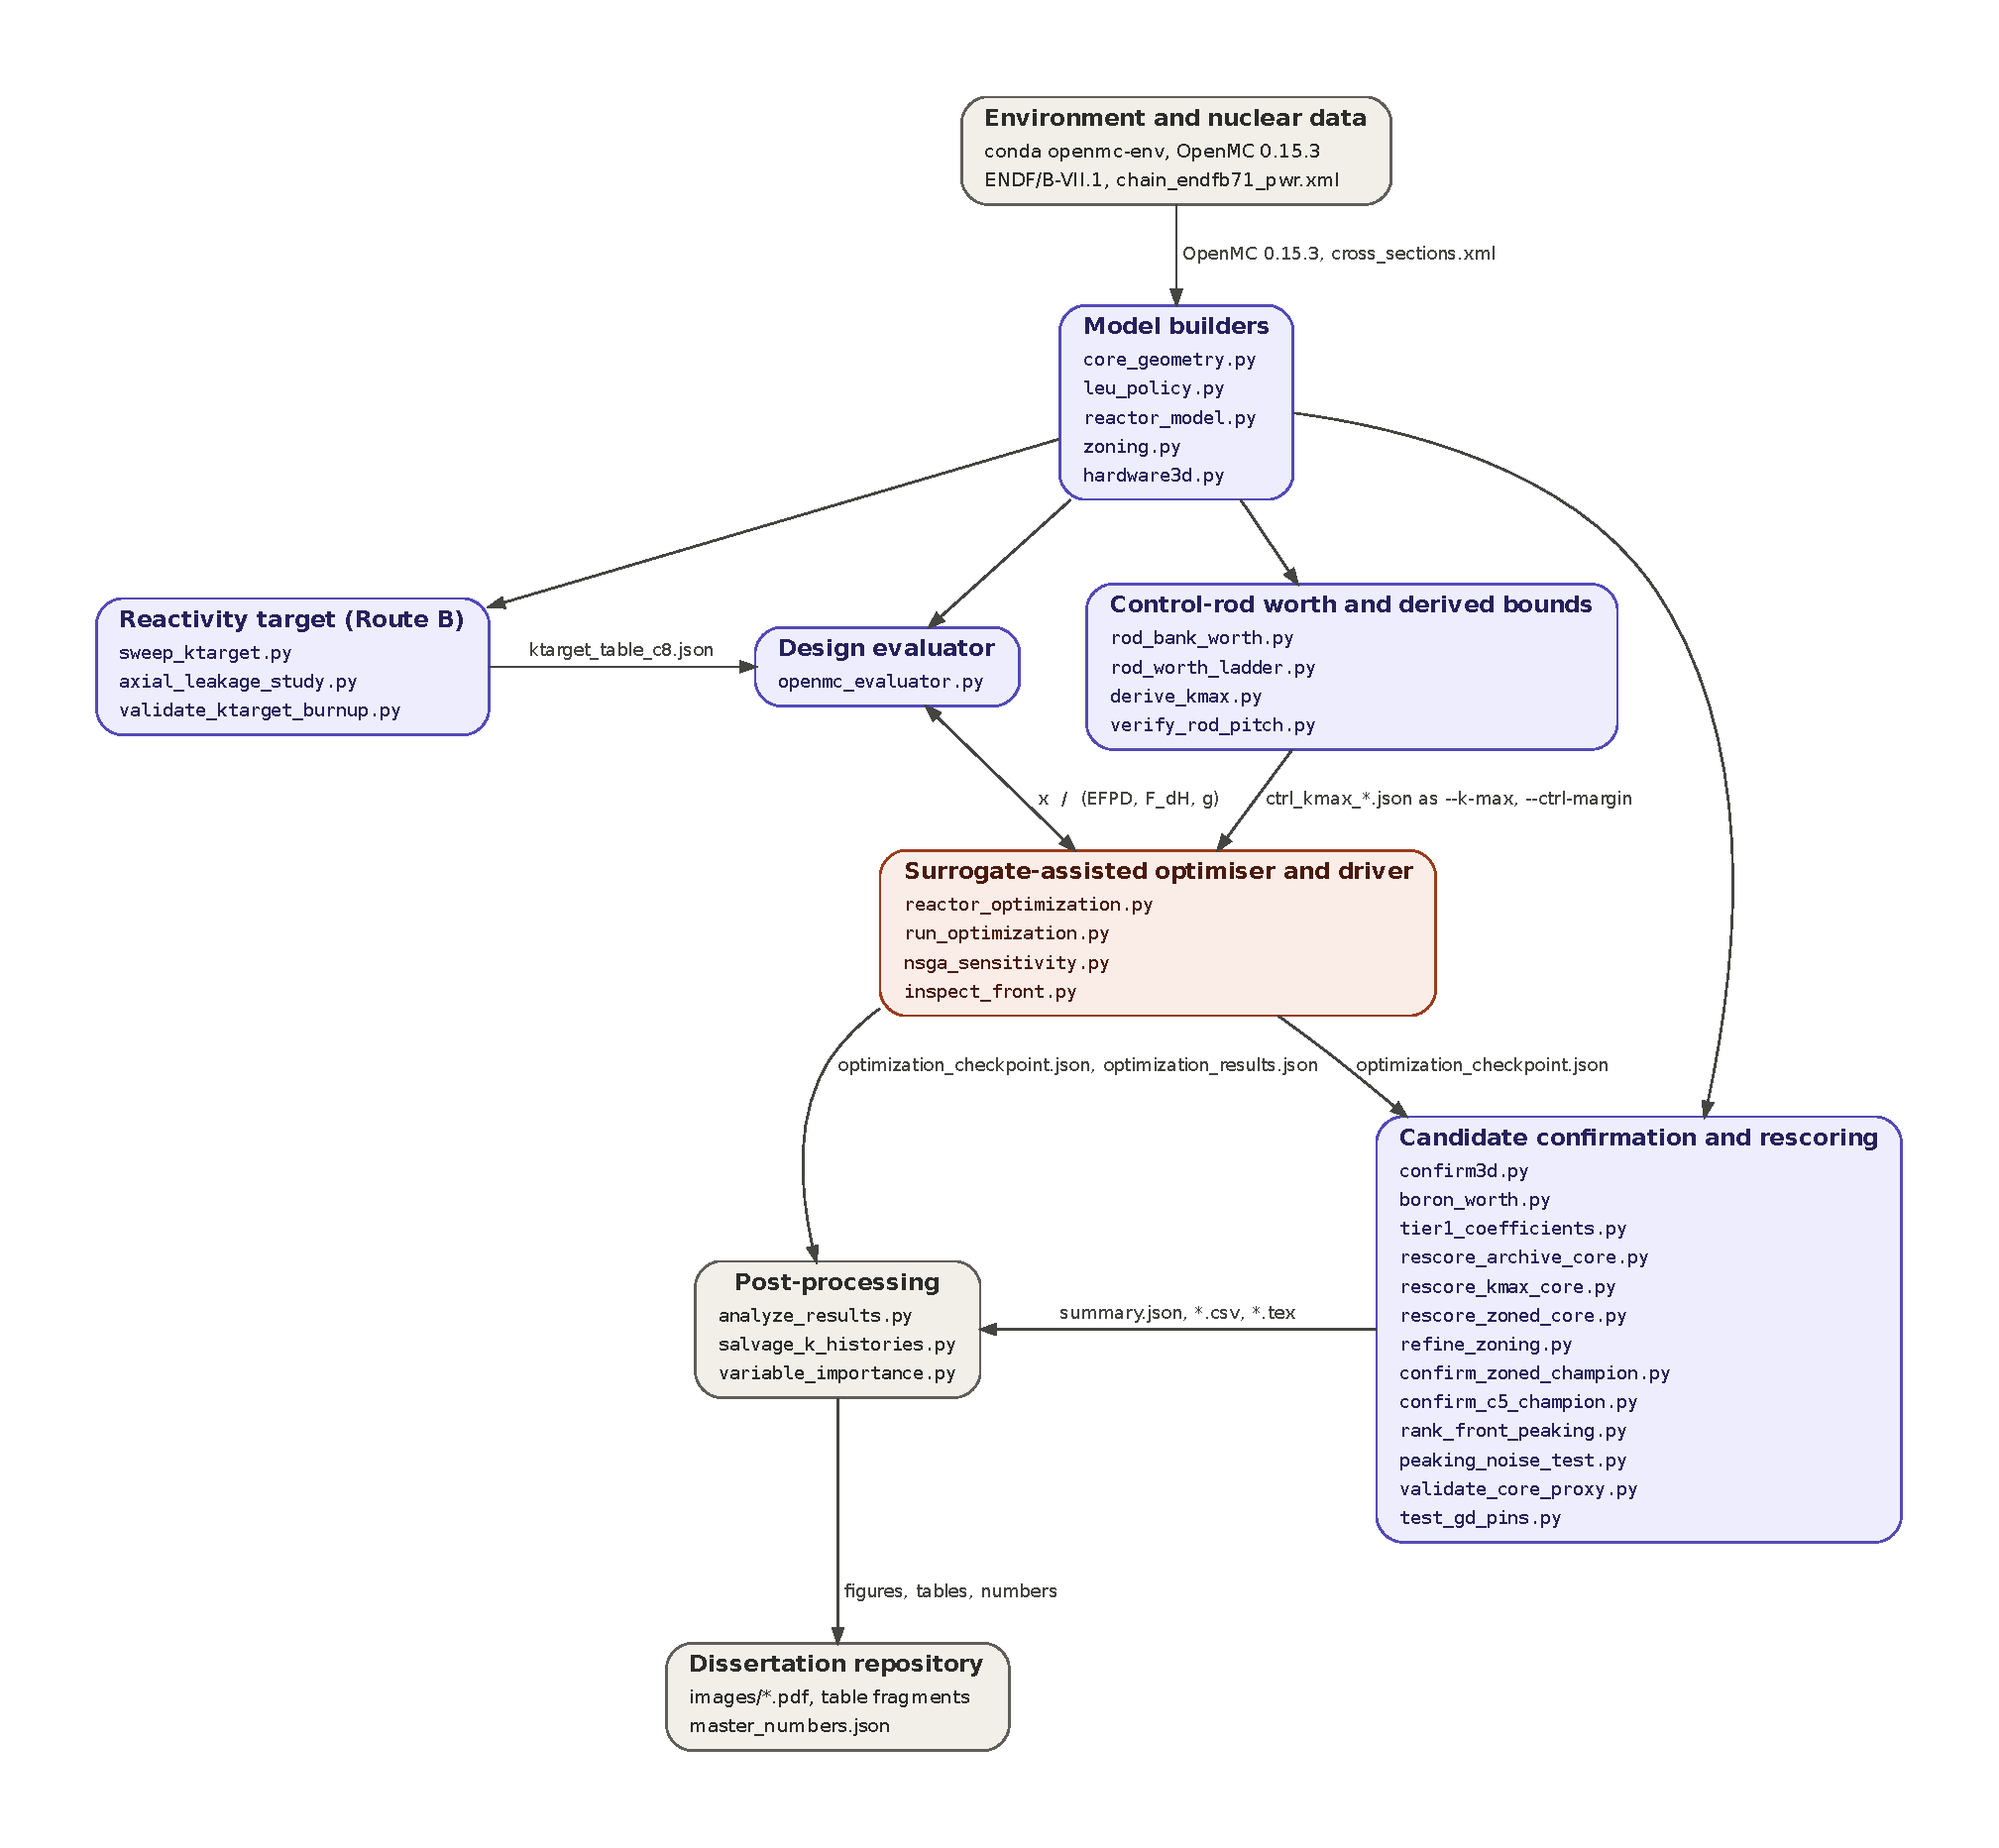
\includegraphics[width=\linewidth]{images/code_architecture.pdf}
  \caption{Macro architecture of the simulation code. Purple blocks run
  OpenMC, the coral block runs the surrogate-assisted optimiser, gray blocks
  are infrastructure and outputs. Scripts listed inside each block are
  detailed in Tables~\ref{tab:arch-builders} to \ref{tab:arch-post}.}
  \label{fig:code-architecture}
\end{figure}

One campaign traverses the blocks in the following order.

\begin{enumerate}[nosep]
  \item The reactivity target table and the derived reactivity ceiling are
        computed once, before the campaign, by the reactivity-target block
        and the control-rod block.
  \item The driver samples the Design of Experiments (DOE) by Latin
        Hypercube Sampling (LHS) \cite{mckay_lhs_1979} and sends each design
        vector to the evaluator.
  \item The evaluator builds the OpenMC models, runs the assembly depletion
        and the core solves, and returns the objectives and the constraint
        vector.
  \item The optimiser fits the Gaussian Process (GP) surrogates
        \cite{rasmussen_gp_2006}, runs the Non-dominated Sorting Genetic
        Algorithm II (NSGA-II) \cite{deb_nsga2_2002} on the surrogates, and
        selects the infill batch. Steps 3 and 4 repeat for each block of
        iterations.
  \item The confirmation block re-evaluates the archived candidates at
        higher fidelity, in three dimensions, and with the control and boron
        studies.
  \item The post-processing block extracts the front, the hypervolume
        history and the corrected depletion histories, and feeds the
        dissertation repository.
\end{enumerate}

\section{Blocks}

\subsection{Environment and nuclear data}

All physics blocks run inside one conda environment, \texttt{openmc-env},
pinned by \texttt{environment.yml} and reproduced in a Docker image by the
\texttt{Dockerfile}. The environment provides OpenMC 0.15.3
\cite{romano_openmc_2015,romano_2021_depletion}, pymoo 0.6.2
\cite{blank_deb_2020} and scikit-learn \cite{pedregosa_sklearn_2011}.

The nuclear data are the ENDF/B-VII.1 continuous-energy cross sections
\cite{chadwick_endf71_2011} and the depletion chain
\file{chain_endfb71_pwr.xml}, downloaded once per machine by
\texttt{setup\_data.sh}. Every script resolves the cross sections through
the environment variable \texttt{OPENMC\_CROSS\_SECTIONS} and the depletion
chain through \texttt{OPENMC\_CHAIN\_FILE}, so no path is written in the
source.

\subsection{Model builders}

This block holds the five library modules that every physics script
imports. They contain no command-line interface and write no result file.
Their outputs are OpenMC model objects, built in memory from a design
dictionary.

\begin{table}[htbp]
  \centering\footnotesize
  \caption{Model builders. These modules are imported, never run.}
  \label{tab:arch-builders}
  \begin{tabularx}{\linewidth}{@{}>{\raggedright\arraybackslash}p{3.6cm} X@{}}
    \toprule
    Module & Role \\
    \midrule
    \file{core_geometry.py} & Vessel envelope, geometric margin, maximum
      reflector thickness, end-of-cycle crossing of the reactivity history,
      bilinear interpolation of the target table \\
    \file{leu_policy.py} & Enrichment cap and search-box constants, defined
      once so that the search box, the evaluator and the driver cannot
      disagree \\
    \file{reactor_model.py} & Materials, fuel pin, guide tube, control-rod
      universes, $17\times17$ assembly and 32-assembly core builders,
      gadolinium pin pattern \\
    \file{zoning.py} & Ring map, centre, middle and periphery multipliers,
      control-bank positions, core beginning-of-life solve, reactivity
      history reader \\
    \file{hardware3d.py} & Finite-height core with the assembly hardware
      stack, used by the three-dimensional confirmation \\
    \bottomrule
  \end{tabularx}
\end{table}

\subsection{Reactivity target (Route B)}

This block produces the end-of-cycle reactivity target used by the
evaluator, as described in the methodology. The target is tabulated on the
full core, corrected for axial leakage, and validated against the burnup
dependence of the leakage.

\begin{table}[htbp]
  \centering\footnotesize
  \caption{Reactivity-target block. The two validation scripts read the
  campaign checkpoint to select the designs they evaluate.}
  \label{tab:arch-ktarget}
  \begin{tabularx}{\linewidth}{@{}>{\raggedright\arraybackslash}p{5.0cm} X >{\raggedright\arraybackslash}p{4.4cm}@{}}
    \toprule
    Script & Role & Main output \\
    \midrule
    \file{sweep_ktarget.py} & Tabulates the target versus pitch and
      reflector thickness from paired assembly and core solves &
      \file{ktarget_table.json} \\
    \file{axial_leakage_study.py} & Axial leakage factor
      $L_{\mathrm{ax}} = k_{2\mathrm{D}}/k_{3\mathrm{D}}$ on archived designs &
      \file{axial_<absorber>.json} \\
    \file{validate_ktarget_burnup.py} & Burnup dependence of the target on
      the front designs & \file{summary.json} \\
    \bottomrule
  \end{tabularx}
\end{table}

\subsection{Design evaluator}

The evaluator is a single module, \file{openmc_evaluator.py}. It is the
only place where a design vector becomes physics. Its public method
\texttt{evaluate\_one} performs three solves per design and returns the
mapping

\[
  \mathbf{x} = \left(e,\, w_{\mathrm{Gd}},\, t_{\mathrm{refl}},\, n_{\mathrm{Gd}}\right)
  \quad\longmapsto\quad
  \left(T_{\mathrm{EFPD}},\, F_{\Delta H},\, \mathbf{g}\right)
\]

\begin{description}[nosep]
  \item[$e$] fuel enrichment, in weight percent of \isotope[235]{U}
  \item[$w_{\mathrm{Gd}}$] gadolinia loading of the poisoned pins, in weight percent
  \item[$t_{\mathrm{refl}}$] radial reflector thickness, in cm
  \item[$n_{\mathrm{Gd}}$] number of poisoned pins per assembly, dimensionless
  \item[$T_{\mathrm{EFPD}}$] cycle length, in effective full power days
  \item[$F_{\Delta H}$] radial enthalpy-rise hot channel factor, dimensionless
  \item[$\mathbf{g}$] constraint vector on reactivity, enrichment and controllability, each entry normalised by its own limit, dimensionless
\end{description}

The three solves are the two-dimensional assembly depletion, which gives
$T_{\mathrm{EFPD}}$ through the end-of-cycle crossing of the target, the
core beginning-of-life solve, which gives $F_{\Delta H}$ and the core
eigenvalue, and the rodded core solve, which gives the controllability
entries of $\mathbf{g}$. The evaluator reads \file{ktarget_table*.json}
and writes one \file{depletion_results.h5} per case.

\subsection{Control-rod worth and derived bounds}

This block measures the worth of the control banks on archived designs and
turns the minimum worth into the reactivity ceiling passed to the driver.
It runs before a campaign, and again on the candidates after it.

\begin{table}[htbp]
  \centering\footnotesize
  \caption{Control-rod block. All scripts read the campaign checkpoint
  except \texttt{derive\_kmax.py}, which reads the screen written by
  \texttt{rod\_bank\_worth.py}.}
  \label{tab:arch-ctrl}
  \begin{tabularx}{\linewidth}{@{}>{\raggedright\arraybackslash}p{5.0cm} X >{\raggedright\arraybackslash}p{4.4cm}@{}}
    \toprule
    Script & Role & Main output \\
    \midrule
    \file{rod_bank_worth.py} & Bank worths and controllability screen of
      archived designs & \file{banks_<absorber>.json} \\
    \file{rod_worth_ladder.py} & Rod-worth ladder and rodded peaking of the
      zoned core & \file{ladder_idx<i>_}\newline\file{<absorber>.json} \\
    \file{derive_kmax.py} & Reactivity ceiling from the minimum bank worth
      and the controllability margin & \file{ctrl_kmax_<group>.json} \\
    \file{verify_rod_pitch.py} & Guide-tube clipping study versus pin pitch &
      \file{fig_rod_pitch_*.pdf} \\
    \bottomrule
  \end{tabularx}
\end{table}

\subsection{Surrogate-assisted optimiser and driver}

The optimiser holds the design space, the surrogates, the acquisition step
and the checkpoint. The driver exposes it as a command line, records the
provenance of every run in the checkpoint, and refuses to resume a
checkpoint whose settings differ from the current command.

\begin{table}[htbp]
  \centering\footnotesize
  \caption{Optimiser block. The driver reads the target table and, on
  resume, the checkpoint. The two analysis scripts read the checkpoint.}
  \label{tab:arch-optimiser}
  \begin{tabularx}{\linewidth}{@{}>{\raggedright\arraybackslash}p{5.0cm} X >{\raggedright\arraybackslash}p{4.4cm}@{}}
    \toprule
    Script & Role & Main output \\
    \midrule
    \file{reactor_optimization.py} & Design space, GP surrogates, NSGA-II
      acquisition on the surrogates, feasibility margin, batch diversity,
      hypervolume, checkpoint & \file{optimization_}\newline\file{checkpoint.json} \\
    \file{run_optimization.py} & Command-line driver: DOE, blocks of infill
      iterations, resume, provenance & \file{optimization_}\newline\file{results.json} \\
    \file{nsga_sensitivity.py} & Sensitivity of the acquisition step to the
      NSGA-II population, generations and seed & \file{nsga_sensitivity.json} \\
    \file{inspect_front.py} & Census of a live checkpoint: front, screens,
      per-block diversity & \file{<prefix>_front.csv} \\
    \bottomrule
  \end{tabularx}
\end{table}

\subsection{Candidate confirmation and rescoring}

This block re-evaluates archived designs outside the optimisation loop. Its
scripts share one pattern. They read the campaign checkpoint, select
designs by index or by front membership, run OpenMC at a fidelity chosen on
the command line, cache every solve in a \file{runs.json} keyed by design
and state, and write a summary. The cache makes every script resumable.

\begin{table}[htbp]
  \centering\footnotesize
  \caption{Confirmation block. All scripts read the campaign checkpoint.}
  \label{tab:arch-confirm}
  \begin{tabularx}{\linewidth}{@{}>{\raggedright\arraybackslash}p{5.0cm} X >{\raggedright\arraybackslash}p{4.4cm}@{}}
    \toprule
    Script & Role & Main output \\
    \midrule
    \file{confirm3d.py} & Three-dimensional confirmation with the hardware
      stack, several rod states and boron concentrations & \file{summary.json} \\
    \file{boron_worth.py} & Boron worth and share of the beginning-of-life
      hold-down across rod states and concentrations & \file{boron_table.tex} \\
    \file{tier1_coefficients.py} & Reactivity coefficients of a candidate &
      \file{tier1_idx<i>.json} \\
    \file{rescore_archive_core.py} & Core-basis peaking of an assembly-basis
      archive & \file{core_rescore.csv} \\
    \file{rescore_kmax_core.py} & Re-screens a finished campaign on the core
      reactivity limits & \file{<label>_kbasis_}\newline\file{summary.json} \\
    \file{rescore_zoned_core.py} & Transfer test of the zoned loading on an
      archive & \file{transfer_summary.json} \\
    \file{refine_zoning.py} & Refinement of the ring multipliers of a
      champion & \file{runs.json} \\
    \file{confirm_zoned_champion.py} & Depletion of the zoned champion at
      full fidelity & \file{confirm_idx<i>.json} \\
    \file{confirm_c5_champion.py} & Feasibility of the Campaign 5 champion
      at full fidelity & \file{summary.json} \\
    \file{rank_front_peaking.py} & Minimum-$F_{\Delta H}$ design beyond
      Monte Carlo noise, by sequential screening & \file{ranking.csv} \\
    \file{peaking_noise_test.py} & Seed replicates of $F_{\Delta H}$ on the
      front designs & \file{noise_summary.csv} \\
    \file{validate_core_proxy.py} & Assembly-to-core peaking proxy
      validation & \file{core_validation.csv} \\
    \file{test_gd_pins.py} & Gadolinium pin-count test on a champion,
      assembly and core & \file{summary.json} \\
    \bottomrule
  \end{tabularx}
\end{table}

\subsection{Post-processing}

The post-processing block reads the campaign archive and the confirmation
summaries and produces the quantities reported in the results chapters.

\begin{table}[htbp]
  \centering\footnotesize
  \caption{Post-processing block. Figure generators and log parsers are
  omitted, see Section~\ref{sec:arch-scope}.}
  \label{tab:arch-post}
  \begin{tabularx}{\linewidth}{@{}>{\raggedright\arraybackslash}p{5.0cm} X >{\raggedright\arraybackslash}p{4.4cm}@{}}
    \toprule
    Script & Role & Main output \\
    \midrule
    \file{analyze_results.py} & Pareto front, hypervolume history,
      design-space diagnostics & figures \\
    \file{salvage_k_histories.py} & Corrects the archived depletion histories
      for the restart defect of the depletion chunks & \file{salvage_summary.csv} \\
    \file{variable_importance.py} & Permutation importance of the design
      variables on the archive & standard output \\
    \bottomrule
  \end{tabularx}
\end{table}

\subsection{Dissertation repository}

The dissertation is kept in a second repository,
\url{https://github.com/dcrlopes/Masther-Thesis-UNIPI---Di-go-Lopes},
synchronised with Overleaf. Figures are stored under \texttt{images/}.
Every number quoted in the text is taken from
\file{master_numbers.json}, which is the single source of truth for the
thesis.

\openpoint{\file{master_numbers.json} is not under version control in
either repository. It was produced with the computational-cost section and
lives only on the workstation. Commit it to \texttt{results\_timing/} in the
simulation repository before submission, so that the last arrow of
Figure~\ref{fig:code-architecture} points to a file a reader can open.}

\section{Interfaces between blocks}

Table~\ref{tab:arch-interfaces} lists the artefacts that cross the block
boundaries of Figure~\ref{fig:code-architecture}. Every artefact is a
plain text file, JSON or CSV, so that any stage can be inspected without
the code.

\begin{table}[htbp]
  \centering\footnotesize
  \caption{Artefacts exchanged between blocks.}
  \label{tab:arch-interfaces}
  \begin{tabularx}{\linewidth}{@{}>{\raggedright\arraybackslash}p{5.1cm} >{\raggedright\arraybackslash}p{2.1cm} >{\raggedright\arraybackslash}p{2.5cm} X@{}}
    \toprule
    Artefact & Producer & Consumer & Content \\
    \midrule
    \file{ktarget_table_c8.json} & Reactivity target & Evaluator &
      Target $k$ versus pitch and reflector thickness, with the axial
      correction $L_{\mathrm{ax}}$ \\
    \file{ctrl_kmax_<group>.json} & Control-rod worth & Driver &
      Derived ceiling, passed as \texttt{--k-max} and \texttt{--ctrl-margin} \\
    design vector $\mathbf{x}$ & Optimiser & Evaluator &
      One design per call \\
    $(T_{\mathrm{EFPD}}, F_{\Delta H}, \mathbf{g})$ & Evaluator & Optimiser &
      Objectives and normalised constraints \\
    \file{optimization_checkpoint.json} & Optimiser & Confirmation,
      post-processing & Every evaluation of the campaign with its
      provenance \\
    \file{optimization_results.json} & Optimiser & Post-processing &
      Front, raw objectives, hypervolume history \\
    \file{summary.json}, \file{*.csv} & Confirmation & Post-processing &
      Per-design results of each confirmation study \\
    \file{images/*.pdf}, \file{*.tex} & Post-processing & Dissertation &
      Figures and table fragments \\
    \bottomrule
  \end{tabularx}
\end{table}

The checkpoint is the central artefact. It is written at the end of every
block of iterations and it records the design space, the constraint
definition, the transport fidelity, the target table and the command line.
A resumed run compares these fields with its own arguments and warns on any
difference. All confirmation and post-processing scripts read the
checkpoint, never the raw case directories, so a campaign can be
re-analysed from a single file.

\openpoint{Regenerate the table of Section~1 of the repository
\texttt{README.md} with \texttt{make\_architecture\_figure.py --table md},
because the current table describes the Campaign 3 layout.}
                       (add this line)
%%   \end{appendices}
%%
%% Figure: images/code_architecture.pdf, produced by
%% make_architecture_figure.py in the simulation repository. Regenerate the
%% figure and the table rows (--table latex) whenever a script is added.
%%
%% New bibliography entries required (appended to references_additions.bib):
%%   pedregosa_sklearn_2011, chadwick_endf71_2011
%% ---------------------------------------------------------------------

\chapter{Architecture of the simulation code}\label{app:code-architecture}

\providecommand{\file}[1]{\texttt{\detokenize{#1}}}

\providecommand{\openpoint}[1]{\par\noindent\fbox{\parbox{0.97\linewidth}{%
  \small\textbf{Open point.} #1}}\par}

\section{Purpose and scope}\label{sec:arch-scope}

This appendix documents the organisation of the code that produced every
result in this thesis. It is written for a reader who needs to locate the
script behind a number, reproduce a campaign, or extend the pipeline to
another core.

The code is public. It is hosted at
\url{https://github.com/dcrlopes/master-thesis-unipi}, on the branch
\texttt{campaign8}, which is the state used for the final campaign and for
the candidate confirmation runs. The state described in this appendix is
commit \texttt{22bad3d} of 3 September 2026.

\openpoint{Update the commit hash above to the final state of branch
\texttt{campaign8} at submission. The branch \texttt{main} still holds the
Campaign 3 state of the code and must not be cited.}

The repository contains 92 Python scripts and 8 shell wrappers. Only the
scripts that perform a computation reported in the thesis are described
here. The following groups are omitted on purpose.

\begin{itemize}[nosep]
  \item Shell wrappers for launch, resume and monitoring.
  \item Anchor-verified patch scripts (\texttt{apply\_*.py},
        \texttt{fix\_*.py}, \texttt{repair\_*.py}) that modified the source
        between campaigns. Their role is described in the methodology.
  \item Figure generators, log parsers and timing accounting scripts.
  \item Unit tests, diagnostics and scripts superseded by a later version.
\end{itemize}

\section{Macro architecture}

Figure~\ref{fig:code-architecture} shows the nine blocks of the pipeline and
the artefacts that cross each interface. Purple blocks call OpenMC
\cite{romano_openmc_2015}, the Monte Carlo transport and depletion code.
The coral block is the only one that never calls OpenMC directly. Gray
blocks are infrastructure and outputs. Unlabelled arrows are Python
imports. Labelled arrows name the file, or the pair of vectors, exchanged.

\begin{figure}[htbp]
  \centering
  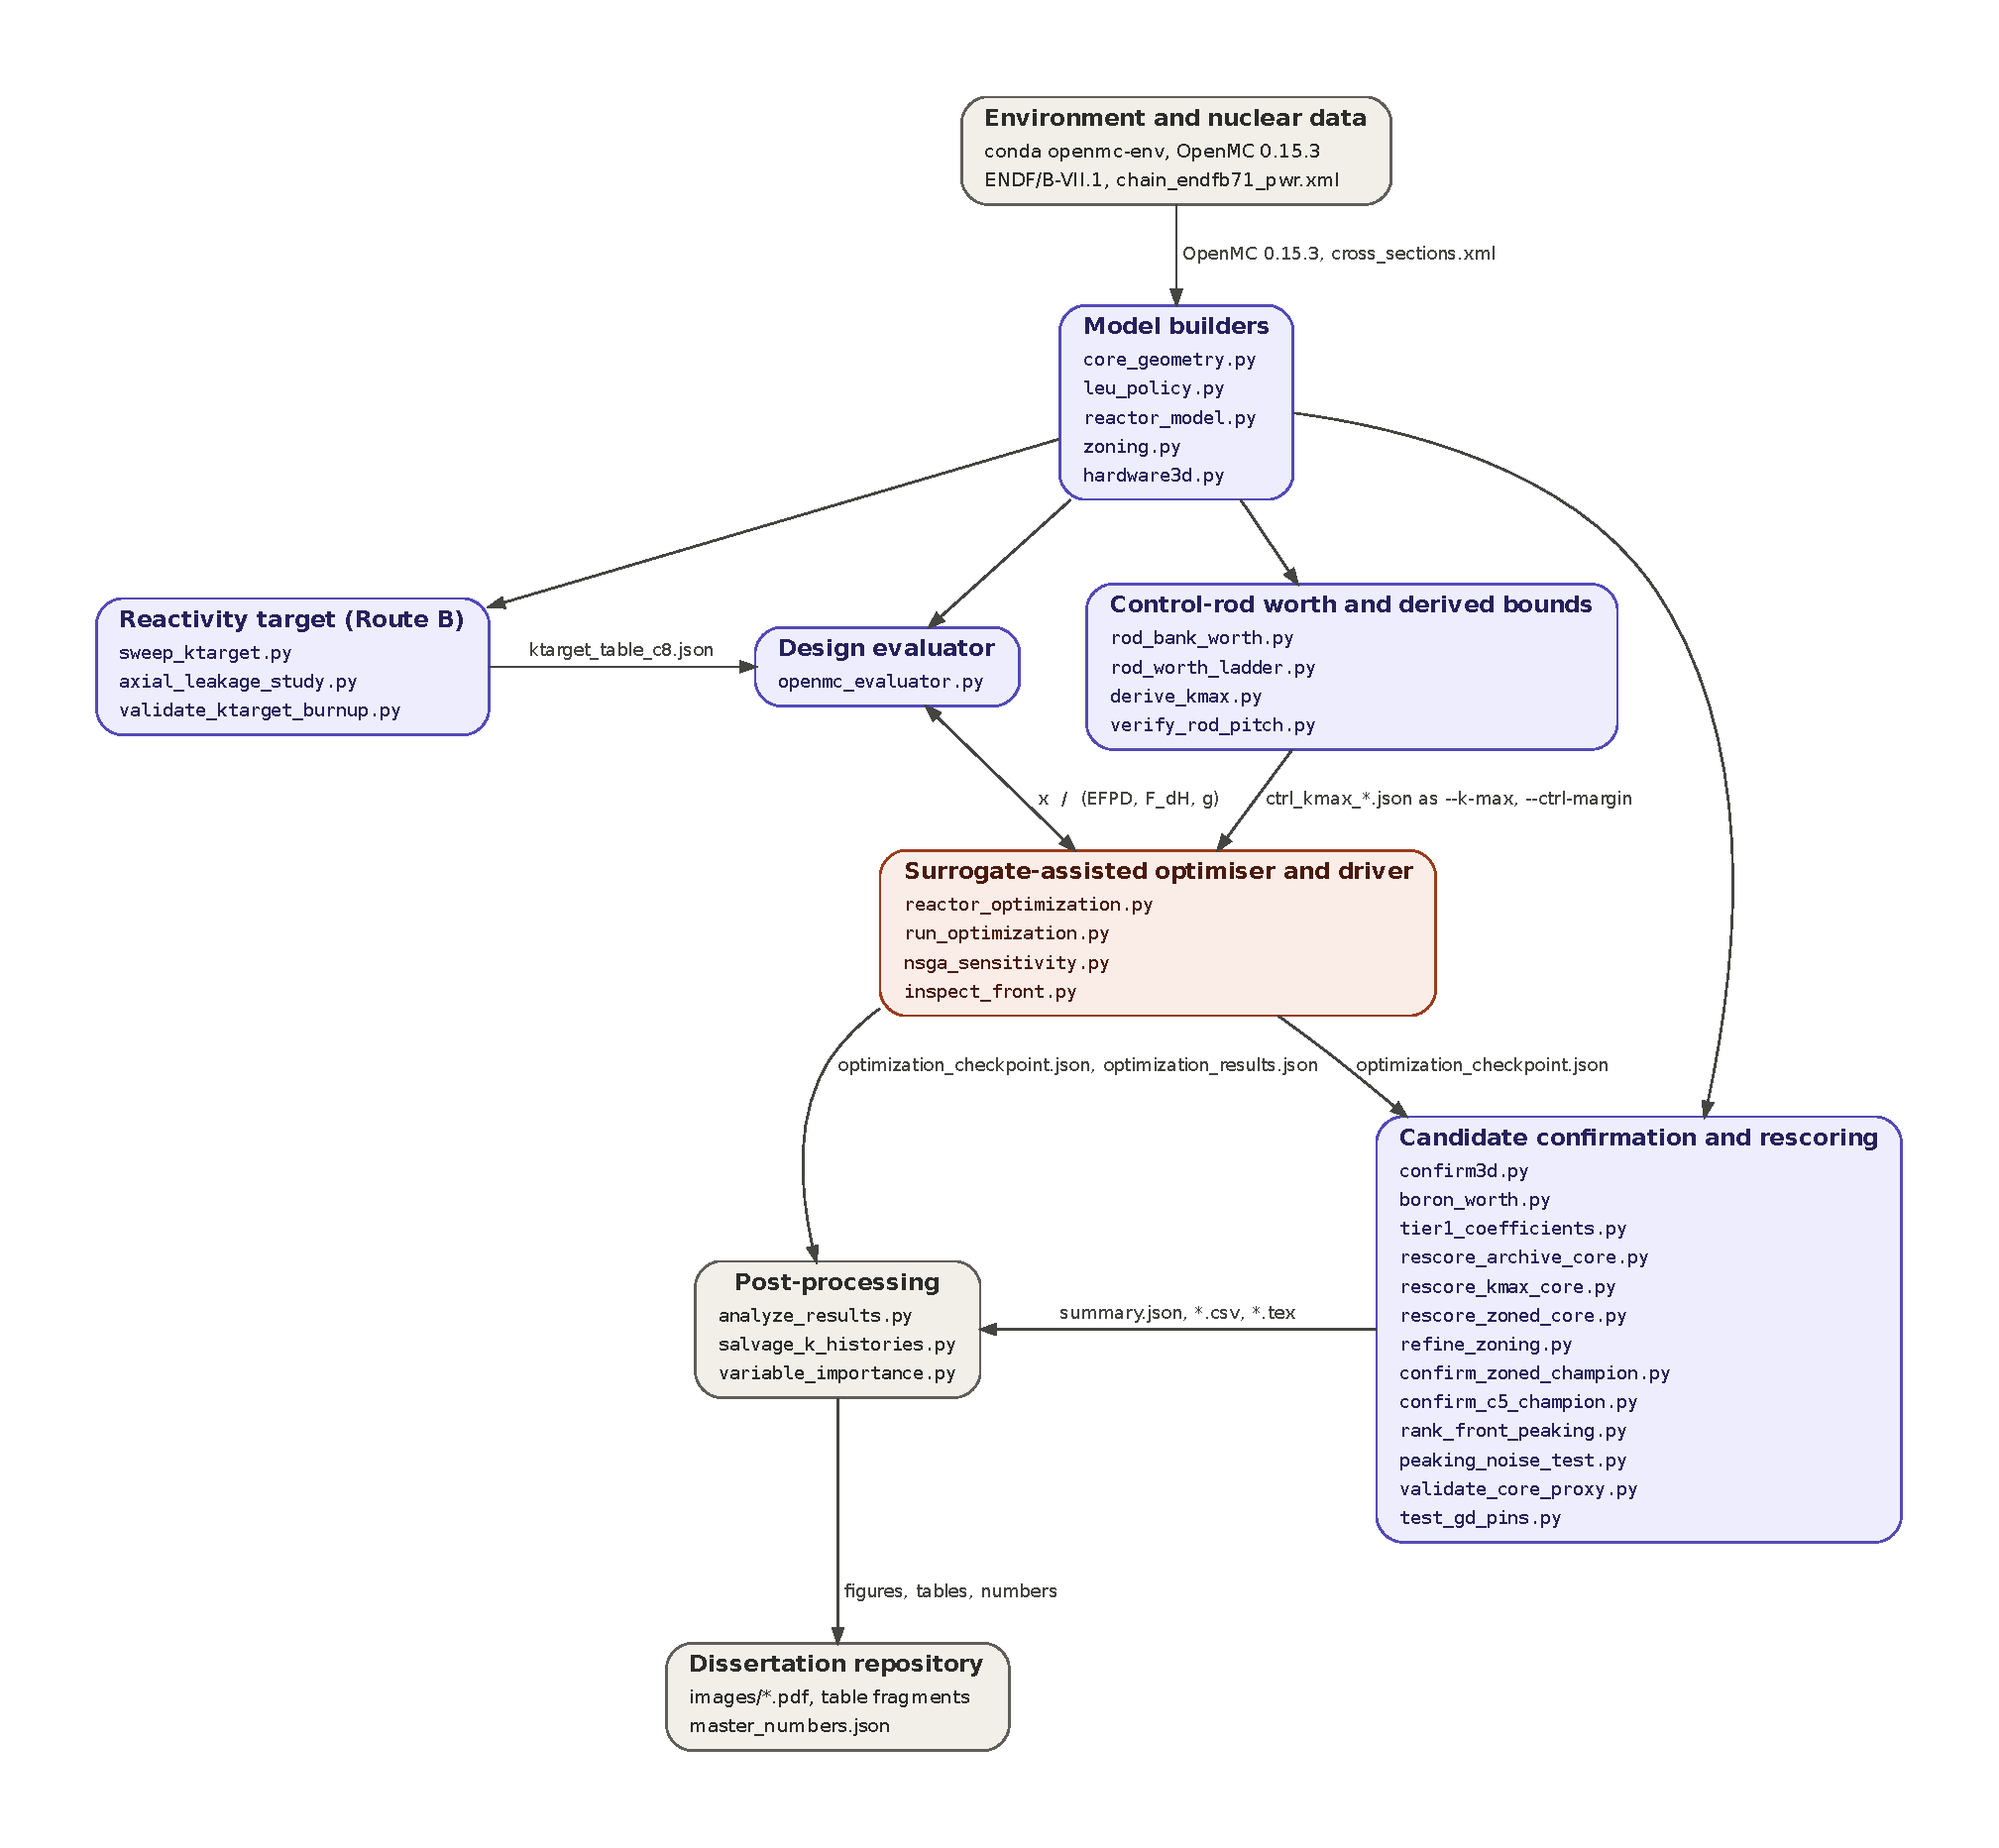
\includegraphics[width=\linewidth]{images/code_architecture.pdf}
  \caption{Macro architecture of the simulation code. Purple blocks run
  OpenMC, the coral block runs the surrogate-assisted optimiser, gray blocks
  are infrastructure and outputs. Scripts listed inside each block are
  detailed in Tables~\ref{tab:arch-builders} to \ref{tab:arch-post}.}
  \label{fig:code-architecture}
\end{figure}

One campaign traverses the blocks in the following order.

\begin{enumerate}[nosep]
  \item The reactivity target table and the derived reactivity ceiling are
        computed once, before the campaign, by the reactivity-target block
        and the control-rod block.
  \item The driver samples the Design of Experiments (DOE) by Latin
        Hypercube Sampling (LHS) \cite{mckay_lhs_1979} and sends each design
        vector to the evaluator.
  \item The evaluator builds the OpenMC models, runs the assembly depletion
        and the core solves, and returns the objectives and the constraint
        vector.
  \item The optimiser fits the Gaussian Process (GP) surrogates
        \cite{rasmussen_gp_2006}, runs the Non-dominated Sorting Genetic
        Algorithm II (NSGA-II) \cite{deb_nsga2_2002} on the surrogates, and
        selects the infill batch. Steps 3 and 4 repeat for each block of
        iterations.
  \item The confirmation block re-evaluates the archived candidates at
        higher fidelity, in three dimensions, and with the control and boron
        studies.
  \item The post-processing block extracts the front, the hypervolume
        history and the corrected depletion histories, and feeds the
        dissertation repository.
\end{enumerate}

\section{Blocks}

\subsection{Environment and nuclear data}

All physics blocks run inside one conda environment, \texttt{openmc-env},
pinned by \texttt{environment.yml} and reproduced in a Docker image by the
\texttt{Dockerfile}. The environment provides OpenMC 0.15.3
\cite{romano_openmc_2015,romano_2021_depletion}, pymoo 0.6.2
\cite{blank_deb_2020} and scikit-learn \cite{pedregosa_sklearn_2011}.

The nuclear data are the ENDF/B-VII.1 continuous-energy cross sections
\cite{chadwick_endf71_2011} and the depletion chain
\file{chain_endfb71_pwr.xml}, downloaded once per machine by
\texttt{setup\_data.sh}. Every script resolves the cross sections through
the environment variable \texttt{OPENMC\_CROSS\_SECTIONS} and the depletion
chain through \texttt{OPENMC\_CHAIN\_FILE}, so no path is written in the
source.

\subsection{Model builders}

This block holds the five library modules that every physics script
imports. They contain no command-line interface and write no result file.
Their outputs are OpenMC model objects, built in memory from a design
dictionary.

\begin{table}[htbp]
  \centering\footnotesize
  \caption{Model builders. These modules are imported, never run.}
  \label{tab:arch-builders}
  \begin{tabularx}{\linewidth}{@{}>{\raggedright\arraybackslash}p{3.6cm} X@{}}
    \toprule
    Module & Role \\
    \midrule
    \file{core_geometry.py} & Vessel envelope, geometric margin, maximum
      reflector thickness, end-of-cycle crossing of the reactivity history,
      bilinear interpolation of the target table \\
    \file{leu_policy.py} & Enrichment cap and search-box constants, defined
      once so that the search box, the evaluator and the driver cannot
      disagree \\
    \file{reactor_model.py} & Materials, fuel pin, guide tube, control-rod
      universes, $17\times17$ assembly and 32-assembly core builders,
      gadolinium pin pattern \\
    \file{zoning.py} & Ring map, centre, middle and periphery multipliers,
      control-bank positions, core beginning-of-life solve, reactivity
      history reader \\
    \file{hardware3d.py} & Finite-height core with the assembly hardware
      stack, used by the three-dimensional confirmation \\
    \bottomrule
  \end{tabularx}
\end{table}

\subsection{Reactivity target (Route B)}

This block produces the end-of-cycle reactivity target used by the
evaluator, as described in the methodology. The target is tabulated on the
full core, corrected for axial leakage, and validated against the burnup
dependence of the leakage.

\begin{table}[htbp]
  \centering\footnotesize
  \caption{Reactivity-target block. The two validation scripts read the
  campaign checkpoint to select the designs they evaluate.}
  \label{tab:arch-ktarget}
  \begin{tabularx}{\linewidth}{@{}>{\raggedright\arraybackslash}p{5.0cm} X >{\raggedright\arraybackslash}p{4.4cm}@{}}
    \toprule
    Script & Role & Main output \\
    \midrule
    \file{sweep_ktarget.py} & Tabulates the target versus pitch and
      reflector thickness from paired assembly and core solves &
      \file{ktarget_table.json} \\
    \file{axial_leakage_study.py} & Axial leakage factor
      $L_{\mathrm{ax}} = k_{2\mathrm{D}}/k_{3\mathrm{D}}$ on archived designs &
      \file{axial_<absorber>.json} \\
    \file{validate_ktarget_burnup.py} & Burnup dependence of the target on
      the front designs & \file{summary.json} \\
    \bottomrule
  \end{tabularx}
\end{table}

\subsection{Design evaluator}

The evaluator is a single module, \file{openmc_evaluator.py}. It is the
only place where a design vector becomes physics. Its public method
\texttt{evaluate\_one} performs three solves per design and returns the
mapping

\[
  \mathbf{x} = \left(e,\, w_{\mathrm{Gd}},\, t_{\mathrm{refl}},\, n_{\mathrm{Gd}}\right)
  \quad\longmapsto\quad
  \left(T_{\mathrm{EFPD}},\, F_{\Delta H},\, \mathbf{g}\right)
\]

\begin{description}[nosep]
  \item[$e$] fuel enrichment, in weight percent of \isotope[235]{U}
  \item[$w_{\mathrm{Gd}}$] gadolinia loading of the poisoned pins, in weight percent
  \item[$t_{\mathrm{refl}}$] radial reflector thickness, in cm
  \item[$n_{\mathrm{Gd}}$] number of poisoned pins per assembly, dimensionless
  \item[$T_{\mathrm{EFPD}}$] cycle length, in effective full power days
  \item[$F_{\Delta H}$] radial enthalpy-rise hot channel factor, dimensionless
  \item[$\mathbf{g}$] constraint vector on reactivity, enrichment and controllability, each entry normalised by its own limit, dimensionless
\end{description}

The three solves are the two-dimensional assembly depletion, which gives
$T_{\mathrm{EFPD}}$ through the end-of-cycle crossing of the target, the
core beginning-of-life solve, which gives $F_{\Delta H}$ and the core
eigenvalue, and the rodded core solve, which gives the controllability
entries of $\mathbf{g}$. The evaluator reads \file{ktarget_table*.json}
and writes one \file{depletion_results.h5} per case.

\subsection{Control-rod worth and derived bounds}

This block measures the worth of the control banks on archived designs and
turns the minimum worth into the reactivity ceiling passed to the driver.
It runs before a campaign, and again on the candidates after it.

\begin{table}[htbp]
  \centering\footnotesize
  \caption{Control-rod block. All scripts read the campaign checkpoint
  except \texttt{derive\_kmax.py}, which reads the screen written by
  \texttt{rod\_bank\_worth.py}.}
  \label{tab:arch-ctrl}
  \begin{tabularx}{\linewidth}{@{}>{\raggedright\arraybackslash}p{5.0cm} X >{\raggedright\arraybackslash}p{4.4cm}@{}}
    \toprule
    Script & Role & Main output \\
    \midrule
    \file{rod_bank_worth.py} & Bank worths and controllability screen of
      archived designs & \file{banks_<absorber>.json} \\
    \file{rod_worth_ladder.py} & Rod-worth ladder and rodded peaking of the
      zoned core & \file{ladder_idx<i>_}\newline\file{<absorber>.json} \\
    \file{derive_kmax.py} & Reactivity ceiling from the minimum bank worth
      and the controllability margin & \file{ctrl_kmax_<group>.json} \\
    \file{verify_rod_pitch.py} & Guide-tube clipping study versus pin pitch &
      \file{fig_rod_pitch_*.pdf} \\
    \bottomrule
  \end{tabularx}
\end{table}

\subsection{Surrogate-assisted optimiser and driver}

The optimiser holds the design space, the surrogates, the acquisition step
and the checkpoint. The driver exposes it as a command line, records the
provenance of every run in the checkpoint, and refuses to resume a
checkpoint whose settings differ from the current command.

\begin{table}[htbp]
  \centering\footnotesize
  \caption{Optimiser block. The driver reads the target table and, on
  resume, the checkpoint. The two analysis scripts read the checkpoint.}
  \label{tab:arch-optimiser}
  \begin{tabularx}{\linewidth}{@{}>{\raggedright\arraybackslash}p{5.0cm} X >{\raggedright\arraybackslash}p{4.4cm}@{}}
    \toprule
    Script & Role & Main output \\
    \midrule
    \file{reactor_optimization.py} & Design space, GP surrogates, NSGA-II
      acquisition on the surrogates, feasibility margin, batch diversity,
      hypervolume, checkpoint & \file{optimization_}\newline\file{checkpoint.json} \\
    \file{run_optimization.py} & Command-line driver: DOE, blocks of infill
      iterations, resume, provenance & \file{optimization_}\newline\file{results.json} \\
    \file{nsga_sensitivity.py} & Sensitivity of the acquisition step to the
      NSGA-II population, generations and seed & \file{nsga_sensitivity.json} \\
    \file{inspect_front.py} & Census of a live checkpoint: front, screens,
      per-block diversity & \file{<prefix>_front.csv} \\
    \bottomrule
  \end{tabularx}
\end{table}

\subsection{Candidate confirmation and rescoring}

This block re-evaluates archived designs outside the optimisation loop. Its
scripts share one pattern. They read the campaign checkpoint, select
designs by index or by front membership, run OpenMC at a fidelity chosen on
the command line, cache every solve in a \file{runs.json} keyed by design
and state, and write a summary. The cache makes every script resumable.

\begin{table}[htbp]
  \centering\footnotesize
  \caption{Confirmation block. All scripts read the campaign checkpoint.}
  \label{tab:arch-confirm}
  \begin{tabularx}{\linewidth}{@{}>{\raggedright\arraybackslash}p{5.0cm} X >{\raggedright\arraybackslash}p{4.4cm}@{}}
    \toprule
    Script & Role & Main output \\
    \midrule
    \file{confirm3d.py} & Three-dimensional confirmation with the hardware
      stack, several rod states and boron concentrations & \file{summary.json} \\
    \file{boron_worth.py} & Boron worth and share of the beginning-of-life
      hold-down across rod states and concentrations & \file{boron_table.tex} \\
    \file{tier1_coefficients.py} & Reactivity coefficients of a candidate &
      \file{tier1_idx<i>.json} \\
    \file{rescore_archive_core.py} & Core-basis peaking of an assembly-basis
      archive & \file{core_rescore.csv} \\
    \file{rescore_kmax_core.py} & Re-screens a finished campaign on the core
      reactivity limits & \file{<label>_kbasis_}\newline\file{summary.json} \\
    \file{rescore_zoned_core.py} & Transfer test of the zoned loading on an
      archive & \file{transfer_summary.json} \\
    \file{refine_zoning.py} & Refinement of the ring multipliers of a
      champion & \file{runs.json} \\
    \file{confirm_zoned_champion.py} & Depletion of the zoned champion at
      full fidelity & \file{confirm_idx<i>.json} \\
    \file{confirm_c5_champion.py} & Feasibility of the Campaign 5 champion
      at full fidelity & \file{summary.json} \\
    \file{rank_front_peaking.py} & Minimum-$F_{\Delta H}$ design beyond
      Monte Carlo noise, by sequential screening & \file{ranking.csv} \\
    \file{peaking_noise_test.py} & Seed replicates of $F_{\Delta H}$ on the
      front designs & \file{noise_summary.csv} \\
    \file{validate_core_proxy.py} & Assembly-to-core peaking proxy
      validation & \file{core_validation.csv} \\
    \file{test_gd_pins.py} & Gadolinium pin-count test on a champion,
      assembly and core & \file{summary.json} \\
    \bottomrule
  \end{tabularx}
\end{table}

\subsection{Post-processing}

The post-processing block reads the campaign archive and the confirmation
summaries and produces the quantities reported in the results chapters.

\begin{table}[htbp]
  \centering\footnotesize
  \caption{Post-processing block. Figure generators and log parsers are
  omitted, see Section~\ref{sec:arch-scope}.}
  \label{tab:arch-post}
  \begin{tabularx}{\linewidth}{@{}>{\raggedright\arraybackslash}p{5.0cm} X >{\raggedright\arraybackslash}p{4.4cm}@{}}
    \toprule
    Script & Role & Main output \\
    \midrule
    \file{analyze_results.py} & Pareto front, hypervolume history,
      design-space diagnostics & figures \\
    \file{salvage_k_histories.py} & Corrects the archived depletion histories
      for the restart defect of the depletion chunks & \file{salvage_summary.csv} \\
    \file{variable_importance.py} & Permutation importance of the design
      variables on the archive & standard output \\
    \bottomrule
  \end{tabularx}
\end{table}

\subsection{Dissertation repository}

The dissertation is kept in a second repository,
\url{https://github.com/dcrlopes/Masther-Thesis-UNIPI---Di-go-Lopes},
synchronised with Overleaf. Figures are stored under \texttt{images/}.
Every number quoted in the text is taken from
\file{master_numbers.json}, which is the single source of truth for the
thesis.

\openpoint{\file{master_numbers.json} is not under version control in
either repository. It was produced with the computational-cost section and
lives only on the workstation. Commit it to \texttt{results\_timing/} in the
simulation repository before submission, so that the last arrow of
Figure~\ref{fig:code-architecture} points to a file a reader can open.}

\section{Interfaces between blocks}

Table~\ref{tab:arch-interfaces} lists the artefacts that cross the block
boundaries of Figure~\ref{fig:code-architecture}. Every artefact is a
plain text file, JSON or CSV, so that any stage can be inspected without
the code.

\begin{table}[htbp]
  \centering\footnotesize
  \caption{Artefacts exchanged between blocks.}
  \label{tab:arch-interfaces}
  \begin{tabularx}{\linewidth}{@{}>{\raggedright\arraybackslash}p{5.1cm} >{\raggedright\arraybackslash}p{2.1cm} >{\raggedright\arraybackslash}p{2.5cm} X@{}}
    \toprule
    Artefact & Producer & Consumer & Content \\
    \midrule
    \file{ktarget_table_c8.json} & Reactivity target & Evaluator &
      Target $k$ versus pitch and reflector thickness, with the axial
      correction $L_{\mathrm{ax}}$ \\
    \file{ctrl_kmax_<group>.json} & Control-rod worth & Driver &
      Derived ceiling, passed as \texttt{--k-max} and \texttt{--ctrl-margin} \\
    design vector $\mathbf{x}$ & Optimiser & Evaluator &
      One design per call \\
    $(T_{\mathrm{EFPD}}, F_{\Delta H}, \mathbf{g})$ & Evaluator & Optimiser &
      Objectives and normalised constraints \\
    \file{optimization_checkpoint.json} & Optimiser & Confirmation,
      post-processing & Every evaluation of the campaign with its
      provenance \\
    \file{optimization_results.json} & Optimiser & Post-processing &
      Front, raw objectives, hypervolume history \\
    \file{summary.json}, \file{*.csv} & Confirmation & Post-processing &
      Per-design results of each confirmation study \\
    \file{images/*.pdf}, \file{*.tex} & Post-processing & Dissertation &
      Figures and table fragments \\
    \bottomrule
  \end{tabularx}
\end{table}

The checkpoint is the central artefact. It is written at the end of every
block of iterations and it records the design space, the constraint
definition, the transport fidelity, the target table and the command line.
A resumed run compares these fields with its own arguments and warns on any
difference. All confirmation and post-processing scripts read the
checkpoint, never the raw case directories, so a campaign can be
re-analysed from a single file.

\openpoint{Regenerate the table of Section~1 of the repository
\texttt{README.md} with \texttt{make\_architecture\_figure.py --table md},
because the current table describes the Campaign 3 layout.}
                       (add this line)
%%   \end{appendices}
%%
%% Figure: images/code_architecture.pdf, produced by
%% make_architecture_figure.py in the simulation repository. Regenerate the
%% figure and the table rows (--table latex) whenever a script is added.
%%
%% New bibliography entries required (appended to references_additions.bib):
%%   pedregosa_sklearn_2011, chadwick_endf71_2011
%% ---------------------------------------------------------------------

\chapter{Architecture of the simulation code}\label{app:code-architecture}

\providecommand{\file}[1]{\texttt{\detokenize{#1}}}

\providecommand{\openpoint}[1]{\par\noindent\fbox{\parbox{0.97\linewidth}{%
  \small\textbf{Open point.} #1}}\par}

\section{Purpose and scope}\label{sec:arch-scope}

This appendix documents the organisation of the code that produced every
result in this thesis. It is written for a reader who needs to locate the
script behind a number, reproduce a campaign, or extend the pipeline to
another core.

The code is public. It is hosted at
\url{https://github.com/dcrlopes/master-thesis-unipi}, on the branch
\texttt{campaign8}, which is the state used for the final campaign and for
the candidate confirmation runs. The state described in this appendix is
commit \texttt{22bad3d} of 3 September 2026.

\openpoint{Update the commit hash above to the final state of branch
\texttt{campaign8} at submission. The branch \texttt{main} still holds the
Campaign 3 state of the code and must not be cited.}

The repository contains 92 Python scripts and 8 shell wrappers. Only the
scripts that perform a computation reported in the thesis are described
here. The following groups are omitted on purpose.

\begin{itemize}[nosep]
  \item Shell wrappers for launch, resume and monitoring.
  \item Anchor-verified patch scripts (\texttt{apply\_*.py},
        \texttt{fix\_*.py}, \texttt{repair\_*.py}) that modified the source
        between campaigns. Their role is described in the methodology.
  \item Figure generators, log parsers and timing accounting scripts.
  \item Unit tests, diagnostics and scripts superseded by a later version.
\end{itemize}

\section{Macro architecture}

Figure~\ref{fig:code-architecture} shows the nine blocks of the pipeline and
the artefacts that cross each interface. Purple blocks call OpenMC
\cite{romano_openmc_2015}, the Monte Carlo transport and depletion code.
The coral block is the only one that never calls OpenMC directly. Gray
blocks are infrastructure and outputs. Unlabelled arrows are Python
imports. Labelled arrows name the file, or the pair of vectors, exchanged.

\begin{figure}[htbp]
  \centering
  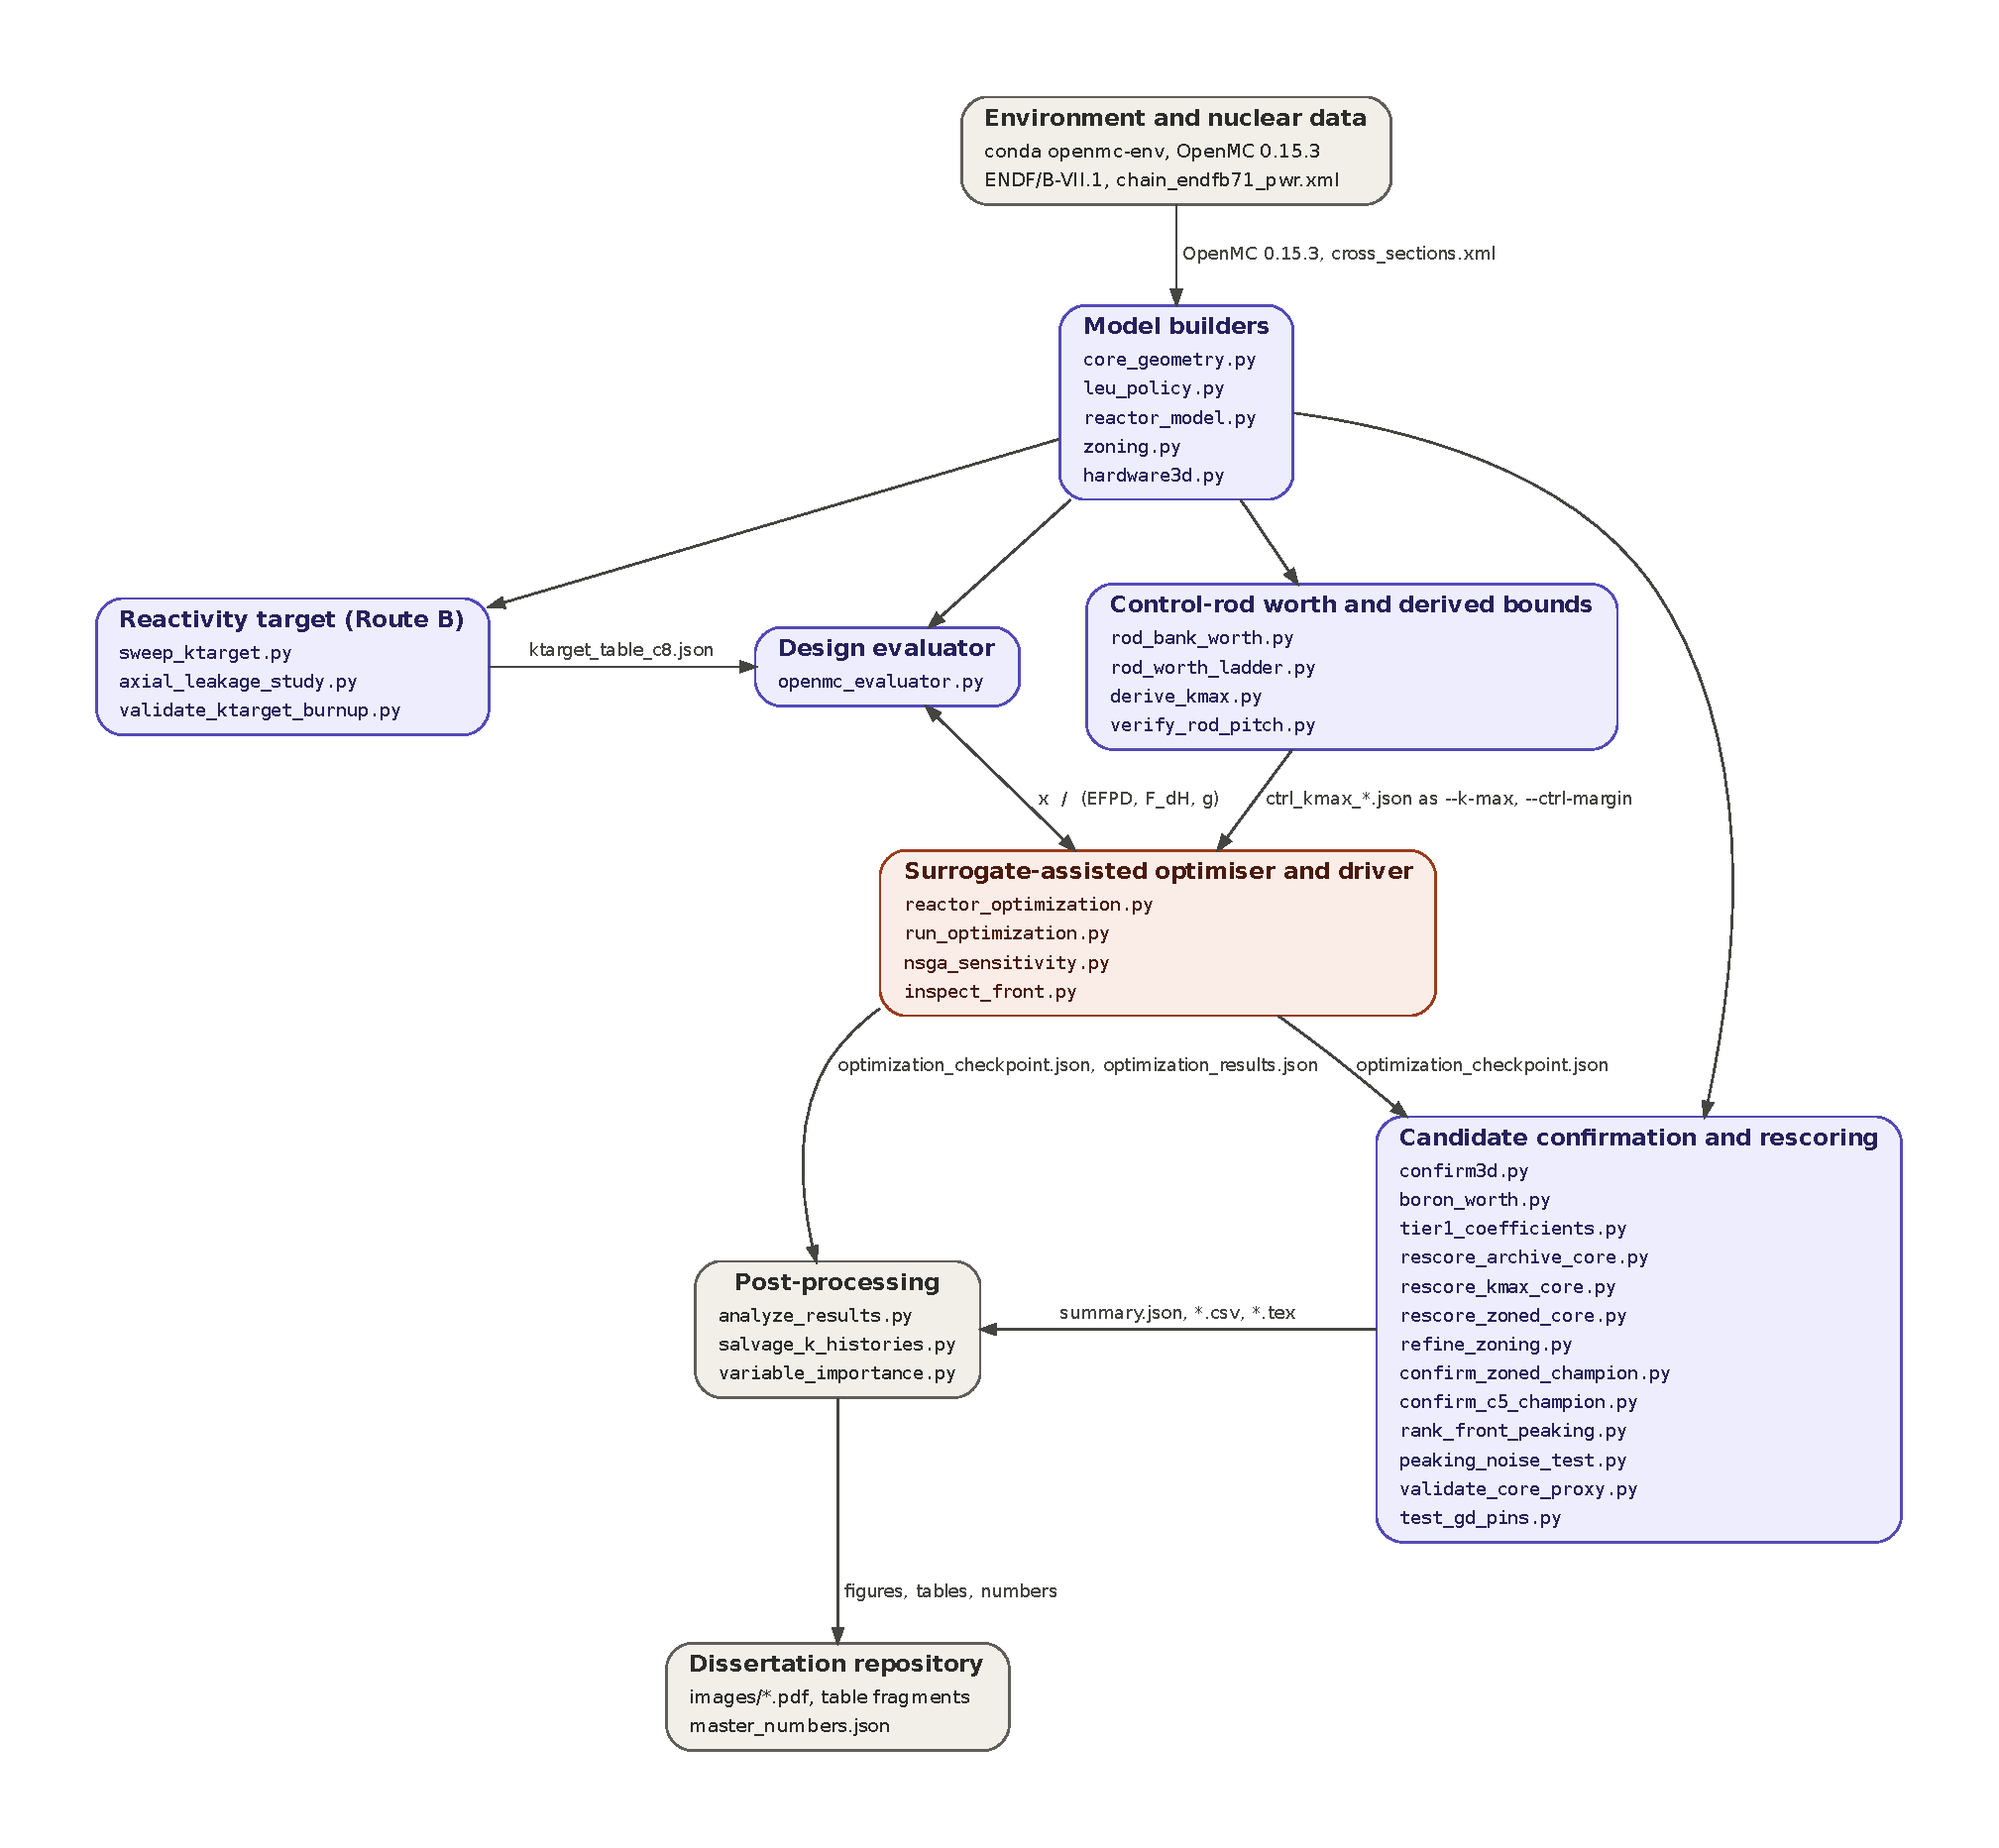
\includegraphics[width=\linewidth]{images/code_architecture.pdf}
  \caption{Macro architecture of the simulation code. Purple blocks run
  OpenMC, the coral block runs the surrogate-assisted optimiser, gray blocks
  are infrastructure and outputs. Scripts listed inside each block are
  detailed in Tables~\ref{tab:arch-builders} to \ref{tab:arch-post}.}
  \label{fig:code-architecture}
\end{figure}

One campaign traverses the blocks in the following order.

\begin{enumerate}[nosep]
  \item The reactivity target table and the derived reactivity ceiling are
        computed once, before the campaign, by the reactivity-target block
        and the control-rod block.
  \item The driver samples the Design of Experiments (DOE) by Latin
        Hypercube Sampling (LHS) \cite{mckay_lhs_1979} and sends each design
        vector to the evaluator.
  \item The evaluator builds the OpenMC models, runs the assembly depletion
        and the core solves, and returns the objectives and the constraint
        vector.
  \item The optimiser fits the Gaussian Process (GP) surrogates
        \cite{rasmussen_gp_2006}, runs the Non-dominated Sorting Genetic
        Algorithm II (NSGA-II) \cite{deb_nsga2_2002} on the surrogates, and
        selects the infill batch. Steps 3 and 4 repeat for each block of
        iterations.
  \item The confirmation block re-evaluates the archived candidates at
        higher fidelity, in three dimensions, and with the control and boron
        studies.
  \item The post-processing block extracts the front, the hypervolume
        history and the corrected depletion histories, and feeds the
        dissertation repository.
\end{enumerate}

\section{Blocks}

\subsection{Environment and nuclear data}

All physics blocks run inside one conda environment, \texttt{openmc-env},
pinned by \texttt{environment.yml} and reproduced in a Docker image by the
\texttt{Dockerfile}. The environment provides OpenMC 0.15.3
\cite{romano_openmc_2015,romano_2021_depletion}, pymoo 0.6.2
\cite{blank_deb_2020} and scikit-learn \cite{pedregosa_sklearn_2011}.

The nuclear data are the ENDF/B-VII.1 continuous-energy cross sections
\cite{chadwick_endf71_2011} and the depletion chain
\file{chain_endfb71_pwr.xml}, downloaded once per machine by
\texttt{setup\_data.sh}. Every script resolves the cross sections through
the environment variable \texttt{OPENMC\_CROSS\_SECTIONS} and the depletion
chain through \texttt{OPENMC\_CHAIN\_FILE}, so no path is written in the
source.

\subsection{Model builders}

This block holds the five library modules that every physics script
imports. They contain no command-line interface and write no result file.
Their outputs are OpenMC model objects, built in memory from a design
dictionary.

\begin{table}[htbp]
  \centering\footnotesize
  \caption{Model builders. These modules are imported, never run.}
  \label{tab:arch-builders}
  \begin{tabularx}{\linewidth}{@{}>{\raggedright\arraybackslash}p{3.6cm} X@{}}
    \toprule
    Module & Role \\
    \midrule
    \file{core_geometry.py} & Vessel envelope, geometric margin, maximum
      reflector thickness, end-of-cycle crossing of the reactivity history,
      bilinear interpolation of the target table \\
    \file{leu_policy.py} & Enrichment cap and search-box constants, defined
      once so that the search box, the evaluator and the driver cannot
      disagree \\
    \file{reactor_model.py} & Materials, fuel pin, guide tube, control-rod
      universes, $17\times17$ assembly and 32-assembly core builders,
      gadolinium pin pattern \\
    \file{zoning.py} & Ring map, centre, middle and periphery multipliers,
      control-bank positions, core beginning-of-life solve, reactivity
      history reader \\
    \file{hardware3d.py} & Finite-height core with the assembly hardware
      stack, used by the three-dimensional confirmation \\
    \bottomrule
  \end{tabularx}
\end{table}

\subsection{Reactivity target (Route B)}

This block produces the end-of-cycle reactivity target used by the
evaluator, as described in the methodology. The target is tabulated on the
full core, corrected for axial leakage, and validated against the burnup
dependence of the leakage.

\begin{table}[htbp]
  \centering\footnotesize
  \caption{Reactivity-target block. The two validation scripts read the
  campaign checkpoint to select the designs they evaluate.}
  \label{tab:arch-ktarget}
  \begin{tabularx}{\linewidth}{@{}>{\raggedright\arraybackslash}p{5.0cm} X >{\raggedright\arraybackslash}p{4.4cm}@{}}
    \toprule
    Script & Role & Main output \\
    \midrule
    \file{sweep_ktarget.py} & Tabulates the target versus pitch and
      reflector thickness from paired assembly and core solves &
      \file{ktarget_table.json} \\
    \file{axial_leakage_study.py} & Axial leakage factor
      $L_{\mathrm{ax}} = k_{2\mathrm{D}}/k_{3\mathrm{D}}$ on archived designs &
      \file{axial_<absorber>.json} \\
    \file{validate_ktarget_burnup.py} & Burnup dependence of the target on
      the front designs & \file{summary.json} \\
    \bottomrule
  \end{tabularx}
\end{table}

\subsection{Design evaluator}

The evaluator is a single module, \file{openmc_evaluator.py}. It is the
only place where a design vector becomes physics. Its public method
\texttt{evaluate\_one} performs three solves per design and returns the
mapping

\[
  \mathbf{x} = \left(e,\, w_{\mathrm{Gd}},\, t_{\mathrm{refl}},\, n_{\mathrm{Gd}}\right)
  \quad\longmapsto\quad
  \left(T_{\mathrm{EFPD}},\, F_{\Delta H},\, \mathbf{g}\right)
\]

\begin{description}[nosep]
  \item[$e$] fuel enrichment, in weight percent of \isotope[235]{U}
  \item[$w_{\mathrm{Gd}}$] gadolinia loading of the poisoned pins, in weight percent
  \item[$t_{\mathrm{refl}}$] radial reflector thickness, in cm
  \item[$n_{\mathrm{Gd}}$] number of poisoned pins per assembly, dimensionless
  \item[$T_{\mathrm{EFPD}}$] cycle length, in effective full power days
  \item[$F_{\Delta H}$] radial enthalpy-rise hot channel factor, dimensionless
  \item[$\mathbf{g}$] constraint vector on reactivity, enrichment and controllability, each entry normalised by its own limit, dimensionless
\end{description}

The three solves are the two-dimensional assembly depletion, which gives
$T_{\mathrm{EFPD}}$ through the end-of-cycle crossing of the target, the
core beginning-of-life solve, which gives $F_{\Delta H}$ and the core
eigenvalue, and the rodded core solve, which gives the controllability
entries of $\mathbf{g}$. The evaluator reads \file{ktarget_table*.json}
and writes one \file{depletion_results.h5} per case.

\subsection{Control-rod worth and derived bounds}

This block measures the worth of the control banks on archived designs and
turns the minimum worth into the reactivity ceiling passed to the driver.
It runs before a campaign, and again on the candidates after it.

\begin{table}[htbp]
  \centering\footnotesize
  \caption{Control-rod block. All scripts read the campaign checkpoint
  except \texttt{derive\_kmax.py}, which reads the screen written by
  \texttt{rod\_bank\_worth.py}.}
  \label{tab:arch-ctrl}
  \begin{tabularx}{\linewidth}{@{}>{\raggedright\arraybackslash}p{5.0cm} X >{\raggedright\arraybackslash}p{4.4cm}@{}}
    \toprule
    Script & Role & Main output \\
    \midrule
    \file{rod_bank_worth.py} & Bank worths and controllability screen of
      archived designs & \file{banks_<absorber>.json} \\
    \file{rod_worth_ladder.py} & Rod-worth ladder and rodded peaking of the
      zoned core & \file{ladder_idx<i>_}\newline\file{<absorber>.json} \\
    \file{derive_kmax.py} & Reactivity ceiling from the minimum bank worth
      and the controllability margin & \file{ctrl_kmax_<group>.json} \\
    \file{verify_rod_pitch.py} & Guide-tube clipping study versus pin pitch &
      \file{fig_rod_pitch_*.pdf} \\
    \bottomrule
  \end{tabularx}
\end{table}

\subsection{Surrogate-assisted optimiser and driver}

The optimiser holds the design space, the surrogates, the acquisition step
and the checkpoint. The driver exposes it as a command line, records the
provenance of every run in the checkpoint, and refuses to resume a
checkpoint whose settings differ from the current command.

\begin{table}[htbp]
  \centering\footnotesize
  \caption{Optimiser block. The driver reads the target table and, on
  resume, the checkpoint. The two analysis scripts read the checkpoint.}
  \label{tab:arch-optimiser}
  \begin{tabularx}{\linewidth}{@{}>{\raggedright\arraybackslash}p{5.0cm} X >{\raggedright\arraybackslash}p{4.4cm}@{}}
    \toprule
    Script & Role & Main output \\
    \midrule
    \file{reactor_optimization.py} & Design space, GP surrogates, NSGA-II
      acquisition on the surrogates, feasibility margin, batch diversity,
      hypervolume, checkpoint & \file{optimization_}\newline\file{checkpoint.json} \\
    \file{run_optimization.py} & Command-line driver: DOE, blocks of infill
      iterations, resume, provenance & \file{optimization_}\newline\file{results.json} \\
    \file{nsga_sensitivity.py} & Sensitivity of the acquisition step to the
      NSGA-II population, generations and seed & \file{nsga_sensitivity.json} \\
    \file{inspect_front.py} & Census of a live checkpoint: front, screens,
      per-block diversity & \file{<prefix>_front.csv} \\
    \bottomrule
  \end{tabularx}
\end{table}

\subsection{Candidate confirmation and rescoring}

This block re-evaluates archived designs outside the optimisation loop. Its
scripts share one pattern. They read the campaign checkpoint, select
designs by index or by front membership, run OpenMC at a fidelity chosen on
the command line, cache every solve in a \file{runs.json} keyed by design
and state, and write a summary. The cache makes every script resumable.

\begin{table}[htbp]
  \centering\footnotesize
  \caption{Confirmation block. All scripts read the campaign checkpoint.}
  \label{tab:arch-confirm}
  \begin{tabularx}{\linewidth}{@{}>{\raggedright\arraybackslash}p{5.0cm} X >{\raggedright\arraybackslash}p{4.4cm}@{}}
    \toprule
    Script & Role & Main output \\
    \midrule
    \file{confirm3d.py} & Three-dimensional confirmation with the hardware
      stack, several rod states and boron concentrations & \file{summary.json} \\
    \file{boron_worth.py} & Boron worth and share of the beginning-of-life
      hold-down across rod states and concentrations & \file{boron_table.tex} \\
    \file{tier1_coefficients.py} & Reactivity coefficients of a candidate &
      \file{tier1_idx<i>.json} \\
    \file{rescore_archive_core.py} & Core-basis peaking of an assembly-basis
      archive & \file{core_rescore.csv} \\
    \file{rescore_kmax_core.py} & Re-screens a finished campaign on the core
      reactivity limits & \file{<label>_kbasis_}\newline\file{summary.json} \\
    \file{rescore_zoned_core.py} & Transfer test of the zoned loading on an
      archive & \file{transfer_summary.json} \\
    \file{refine_zoning.py} & Refinement of the ring multipliers of a
      champion & \file{runs.json} \\
    \file{confirm_zoned_champion.py} & Depletion of the zoned champion at
      full fidelity & \file{confirm_idx<i>.json} \\
    \file{confirm_c5_champion.py} & Feasibility of the Campaign 5 champion
      at full fidelity & \file{summary.json} \\
    \file{rank_front_peaking.py} & Minimum-$F_{\Delta H}$ design beyond
      Monte Carlo noise, by sequential screening & \file{ranking.csv} \\
    \file{peaking_noise_test.py} & Seed replicates of $F_{\Delta H}$ on the
      front designs & \file{noise_summary.csv} \\
    \file{validate_core_proxy.py} & Assembly-to-core peaking proxy
      validation & \file{core_validation.csv} \\
    \file{test_gd_pins.py} & Gadolinium pin-count test on a champion,
      assembly and core & \file{summary.json} \\
    \bottomrule
  \end{tabularx}
\end{table}

\subsection{Post-processing}

The post-processing block reads the campaign archive and the confirmation
summaries and produces the quantities reported in the results chapters.

\begin{table}[htbp]
  \centering\footnotesize
  \caption{Post-processing block. Figure generators and log parsers are
  omitted, see Section~\ref{sec:arch-scope}.}
  \label{tab:arch-post}
  \begin{tabularx}{\linewidth}{@{}>{\raggedright\arraybackslash}p{5.0cm} X >{\raggedright\arraybackslash}p{4.4cm}@{}}
    \toprule
    Script & Role & Main output \\
    \midrule
    \file{analyze_results.py} & Pareto front, hypervolume history,
      design-space diagnostics & figures \\
    \file{salvage_k_histories.py} & Corrects the archived depletion histories
      for the restart defect of the depletion chunks & \file{salvage_summary.csv} \\
    \file{variable_importance.py} & Permutation importance of the design
      variables on the archive & standard output \\
    \bottomrule
  \end{tabularx}
\end{table}

\subsection{Dissertation repository}

The dissertation is kept in a second repository,
\url{https://github.com/dcrlopes/Masther-Thesis-UNIPI---Di-go-Lopes},
synchronised with Overleaf. Figures are stored under \texttt{images/}.
Every number quoted in the text is taken from
\file{master_numbers.json}, which is the single source of truth for the
thesis.

\openpoint{\file{master_numbers.json} is not under version control in
either repository. It was produced with the computational-cost section and
lives only on the workstation. Commit it to \texttt{results\_timing/} in the
simulation repository before submission, so that the last arrow of
Figure~\ref{fig:code-architecture} points to a file a reader can open.}

\section{Interfaces between blocks}

Table~\ref{tab:arch-interfaces} lists the artefacts that cross the block
boundaries of Figure~\ref{fig:code-architecture}. Every artefact is a
plain text file, JSON or CSV, so that any stage can be inspected without
the code.

\begin{table}[htbp]
  \centering\footnotesize
  \caption{Artefacts exchanged between blocks.}
  \label{tab:arch-interfaces}
  \begin{tabularx}{\linewidth}{@{}>{\raggedright\arraybackslash}p{5.1cm} >{\raggedright\arraybackslash}p{2.1cm} >{\raggedright\arraybackslash}p{2.5cm} X@{}}
    \toprule
    Artefact & Producer & Consumer & Content \\
    \midrule
    \file{ktarget_table_c8.json} & Reactivity target & Evaluator &
      Target $k$ versus pitch and reflector thickness, with the axial
      correction $L_{\mathrm{ax}}$ \\
    \file{ctrl_kmax_<group>.json} & Control-rod worth & Driver &
      Derived ceiling, passed as \texttt{--k-max} and \texttt{--ctrl-margin} \\
    design vector $\mathbf{x}$ & Optimiser & Evaluator &
      One design per call \\
    $(T_{\mathrm{EFPD}}, F_{\Delta H}, \mathbf{g})$ & Evaluator & Optimiser &
      Objectives and normalised constraints \\
    \file{optimization_checkpoint.json} & Optimiser & Confirmation,
      post-processing & Every evaluation of the campaign with its
      provenance \\
    \file{optimization_results.json} & Optimiser & Post-processing &
      Front, raw objectives, hypervolume history \\
    \file{summary.json}, \file{*.csv} & Confirmation & Post-processing &
      Per-design results of each confirmation study \\
    \file{images/*.pdf}, \file{*.tex} & Post-processing & Dissertation &
      Figures and table fragments \\
    \bottomrule
  \end{tabularx}
\end{table}

The checkpoint is the central artefact. It is written at the end of every
block of iterations and it records the design space, the constraint
definition, the transport fidelity, the target table and the command line.
A resumed run compares these fields with its own arguments and warns on any
difference. All confirmation and post-processing scripts read the
checkpoint, never the raw case directories, so a campaign can be
re-analysed from a single file.

\openpoint{Regenerate the table of Section~1 of the repository
\texttt{README.md} with \texttt{make\_architecture\_figure.py --table md},
because the current table describes the Campaign 3 layout.}


\end{appendices}

\backmatter
\addcontentsline{toc}{chapter}{\bibname}
\bibliographystyle{unsrtnat}
\bibliography{references_additions}
% The bibliographic references are stored in a separate file: biblio.bib
\

\end{document}